\documentclass[11pt,twoside,openright]{book}
\usepackage{qfbook}
\title{Quantum Fluids in Lean~4}
\author{Xavier Callens}
\hypersetup{pdftitle={Quantum Fluids in Lean 4: a tribute to Henri Godfrin},pdfauthor={Xavier Callens}}
\newcommand{\IfCh}[2]{\IfFileExists{chapters/#1.tex}{#2}{}}
\newcommand{\BookConceptDOI}{10.5281/zenodo.23272153}% concept DOI reserved 2026-10-10 (zenodo_draft_book.json); cite it, never a version DOI
\begin{document}
\frontmatter
\pagestyle{empty}
% ------------------------------------------------------------------ title page
\begin{titlepage}
\begin{tikzpicture}[remember picture,overlay]
  \node[anchor=north,inner sep=0pt] at ([yshift=-0.8in]current page.north) {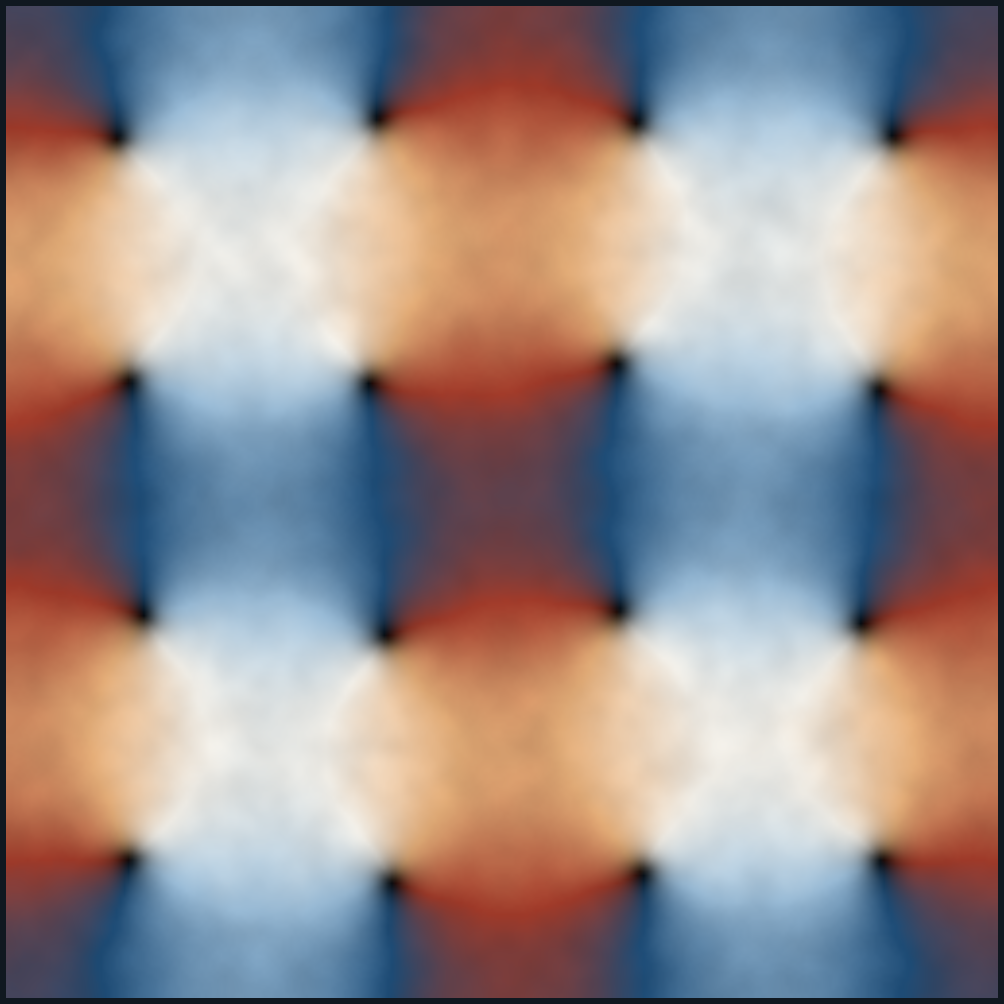
\includegraphics[width=0.50\paperwidth]{figures/cover_frontispiece.png}};
\end{tikzpicture}
\vspace*{3.55in}
\begin{center}
{\color{qfgrey}\scshape\large A tribute to Henri Godfrin}\\[1.6em]
{\fontsize{34}{38}\selectfont\bfseries\color{qfblue} Quantum Fluids\\[0.2em] in Lean~4}\\[1.0em]
{\color{qfgold}\rule{0.45\textwidth}{1.1pt}}\\[1.0em]
{\large\itshape Machine-checked mathematics, solver experiments\\and the measurements of a master experimentalist}\\[1.6em]
{\large Xavier Callens}\\[0.3em]
{\small SocrateAI Research}\\[1.5em]
{\small\color{qfgrey} with the Lean~4 library \texttt{QuantumFluids}\\ and the rusty-SUNDIALS solver (\texttt{qf-pgpe}, CVODE)}\\[0.9em]
{\small\color{qfgrey} October 2026 \enspace $\cdot$ \enspace second edition}
\end{center}
\end{titlepage}
% ------------------------------------------------------------------ colophon (verso of the title page)
\thispagestyle{empty}
\vspace*{\fill}
\begingroup\small\setlength{\parindent}{0pt}\setlength{\parskip}{0.7em}
\textbf{Quantum Fluids in Lean~4: a tribute to Henri Godfrin.}\\
Xavier Callens, SocrateAI Research. Second edition, October 2026; the first edition (October 2026, ten chapters) remains available under doi:\href{https://doi.org/10.5281/zenodo.23272154}{10.5281/zenodo.23272154}.

\textbf{How to cite.} X.~Callens, \emph{Quantum Fluids in Lean~4: a tribute to Henri Godfrin}, SocrateAI Research (2026), doi:\href{https://doi.org/\BookConceptDOI}{\BookConceptDOI}. This is the concept DOI of the book; it always resolves to the latest edition.

\textbf{Licence.} Text and figures: Creative Commons Attribution 4.0 International (CC~BY~4.0). Lean, Python and Rust sources: MIT or Apache-2.0, at the reader's option.

\textbf{Sources.} Every chapter, figure script, number file, Lean file and audit log of this book is in the source archive deposited with it under the DOI above, and in the directory \texttt{book/} of \url{https://github.com/xaviercallens/SocrateAI-Scientific-QuantumFluids}. Lean~4 toolchain \texttt{v4.34.0-rc2}, Mathlib at commit \texttt{85e3a25}. The Lean library \texttt{QuantumFluids} is also archived as software under doi:\href{https://doi.org/10.5281/zenodo.22855581}{10.5281/zenodo.22855581}; the solver is rusty-SUNDIALS, \url{https://github.com/xaviercallens/rusty-SUNDIALS}. Appendix~B says how to rebuild every figure and rerun the Lean audit.

\textbf{A note on the dedication.} Henri Godfrin has not reviewed this book, and nothing in it speaks for him or for his collaborators. The book describes their published measurements; the proofs are proofs of mathematical statements, not of experimental data; every remaining error is the author's.
\endgroup
\cleardoublepage
% ------------------------------------------------------------------ dedication
\thispagestyle{empty}\vspace*{2.2in}
\begin{center}
{\large\itshape To Henri Godfrin,\\[0.6em] and to everyone who builds the cold apparatus\\[0.3em] that lets a quantum fluid answer.}
\end{center}
\cleardoublepage
\pagestyle{fancy}
% ------------------------------------------------------------------ preface
\chapter*{Preface}\addcontentsline{toc}{chapter}{Preface}\markboth{Preface}{Preface}
This book has one idea and one dedication.

The idea is that a quantum fluid can be understood through \emph{three instruments used together}. The first is the experiment: a measurement made at the bench, in a cryostat, on a neutron beam line, in a vacuum chamber of cold atoms. The second is a proof: a statement about the mathematics of the model, checked by a computer so that it cannot be wrong in the way an arithmetic slip or a misprinted coefficient can be wrong. The third is a simulation: a solver that integrates the equations of the model and lets us watch what the proof only asserts. Each instrument is blind where the others see. A proof says nothing about helium; an experiment does not tell you whether a printed formula is right; a simulation cannot distinguish a theorem from a coincidence. Used together, and with their limits stated, they give something firmer than any of them alone.

The dedication is to Henri Godfrin. His group at the Institut N\'eel in Grenoble does the hardest kind of physics: it cools matter to microkelvin temperatures, puts a single atomic layer of helium-3, or a bath of helium-4, in a neutron beam, and reads the excitation spectrum of a quantum fluid directly. The measurements of that programme --- the roton-like collective mode of a two-dimensional Fermi liquid, and the dispersion relation of superfluid helium-4 together with its thermodynamic consequences --- are the experimental thread of this book. Where the Lean library formalizes a statement that appears in his papers, the book says exactly which statement and what the proof does and does not show. Nothing here speaks for him: he has not reviewed this book, the proofs are of mathematics and not of his data, and every error that remains is ours.

The Lean~4 library is \texttt{QuantumFluids}, a collection of machine-checked theorems on the mathematical structure of quantum fluids; the solver is rusty-SUNDIALS, a Rust implementation of the SUNDIALS suite with a quantum-fluids module \texttt{qf-pgpe}. Both belong to a research programme that is run under strict discipline: predictions written before data are read, failures reported, claims retracted when they fail. That discipline shapes the book. Every chapter contains a box that says what is established and what is not, and the last chapter tells, plainly, what went wrong in the programme and how it was found. A tribute to an experimentalist should be written in the register of experimentalists: with the error bars in view.

The book is organized in five parts and fifteen chapters that can be read in order or separately. Part~I (\cref{ch01,ch02}) introduces the three instruments and the measurements that motivate them, and is a primer on Lean and on the solver. Part~II, on Bose superfluids, goes from Bose--Einstein condensation (\cref{ch11}) through circulation and vortices, the specific heat of helium-4 and the dispersion relation to two-fluid hydrodynamics and second sound (\cref{ch12}). Part~III follows the vortices: the Kosterlitz--Thouless flow, friction, Onsager's giant vortex clusters, the flow past an obstacle and quantum turbulence (\cref{ch06,ch07,ch13,ch09,ch15}). Part~IV turns to Fermi fluids: the two-dimensional Fermi liquid with its zero sound and roton mode (\cref{ch08}), and pairing and the superfluidity of helium-3 (\cref{ch14}). Part~V (\cref{ch10}) is about trust. Each chapter takes its theme with a measurement, a theorem and a computation, and ends with three exercises whose worked solutions are in Appendix~C. Appendix~A is the complete catalogue of the Lean library, Appendix~B tells how to rebuild every figure and rerun the audit, and Appendix~D collects the constants, units and notation. Every figure in the book is produced by a script that is part of the source, and every number quoted in the text comes from a file or a computation recorded alongside it.

\paragraph{How the book was made.} The chapters were written separately, each from the same briefing, and combined at the end; the text, the Lean code and the figures were drafted with the assistance of an AI system and then checked: the Lean files compile against the pinned Mathlib, the solver code was run, and the sources of every number are listed in the per-chapter reports kept with the source. The second edition adds five chapters, the solutions of all the exercises and the appendix of constants and notation, made and checked in the same way; the editor's corrections are dated in the briefing files kept with the source. Corrections are welcome.

\begin{flushright}\itshape X.~C.\\ October 2026\end{flushright}

\tableofcontents
\listoffigures
\mainmatter
% ------------------------------------------------------------------ second edition: five parts, chapters in teaching order (file names unchanged)
\part{Foundations}
\IfCh{ch01}{\chapter{A Tribute: The Bench, the Proof and the Solver}\label{ch01}

On 29 March 2012 \emph{Nature} published a spectrum. A neutron beam at the Institut Laue--Langevin (ILL) in Grenoble had been scattered by a single atomic layer of liquid helium-3 adsorbed on graphite, a film that is two-dimensional for every purpose of the physics, and from the neutrons that came out the authors had read the energy of the density waves of the film as a function of their wave number \cite{Godfrin2012}. The curve had a minimum. It was a \emph{roton-like} minimum, a feature long familiar from superfluid helium-4, and here it was found in a Fermi liquid; and the density waves, the collective mode of the film, which enter the band of particle--hole excitations and are strongly damped there, were found to reappear beyond twice the Fermi wave number as a well-defined excitation. Nine years later a second paper with the same first author reported the same kind of measurement on bulk superfluid helium-4, at the ILL spectrometer IN5: the dispersion relation of the Landau elementary excitations, phonon, maxon and roton, and the thermodynamic consequences that follow from it \cite{Godfrin2021}.

A spectrum is the most complete thing one can ask a quantum fluid for. Landau saw in 1941 that at low temperature the thermodynamics of liquid helium is that of a gas of elementary excitations \cite{Landau1941}; the energy of an excitation as a function of its wave number, the \emph{dispersion relation}, is therefore the one curve from which the rest follows, and a neutron beam is the instrument that can draw it. Drawing it takes a sample cooled until it is a quantum fluid, a beam line, and a command of the kinematics of the collision good enough to read a curve out of a cloud of counts. That is a craft. This book tries to honour it in the only way a text can: by saying exactly what the measurements are, why they are hard, and what they settled.

It then does something that the measurements themselves do not ask for: it reads them with three instruments used together. The \emph{bench} is the experiment, a number about nature together with the procedure and the error bar that make it a number. The \emph{proof} is a statement about the mathematics of a model, checked by the proof assistant Lean~4, so that it cannot be wrong in the way a misprinted coefficient can be wrong. The \emph{solver} is rusty-SUNDIALS, a Rust implementation of the SUNDIALS suite of solvers \cite{Hindmarsh2005} with a module for quantum fluids; with it we integrate the equations of a model and watch what a proof only asserts. None of the three can do the work of the others. This chapter says what each can do, shows each at work on an example, and closes with an account of what the two measurements above hand over to theory and of how a companion made of proofs and simulations can be of use to it without presuming to speak for it. The order is the bench (\cref{ch01:sec-bench,ch01:sec-neutron}), the chain from a curve to a calorimeter (\cref{ch01:sec-chain}), the method (\cref{ch01:sec-method}), the proof (\cref{ch01:sec-proof}), the solver (\cref{ch01:sec-solver}) and the handover (\cref{ch01:sec-handover}). \Cref{ch01:fig-timeline} places the two measurements among the landmarks that the book revisits.

\begin{figure}[t]\centering
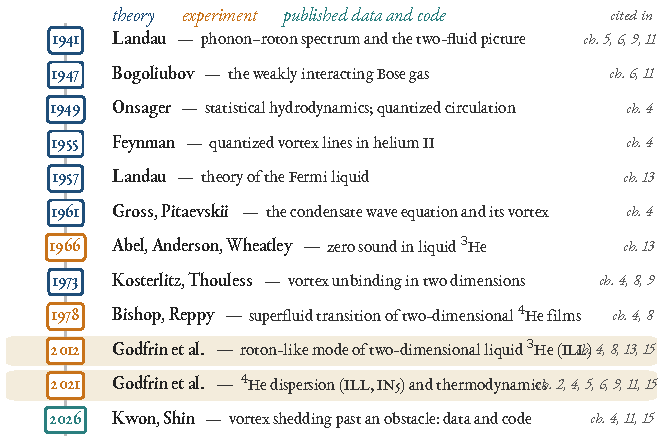
\includegraphics[width=\linewidth]{figures/ch01_timeline.pdf}
\caption[The landmarks this book revisits]{The landmarks this book revisits. Blue: theory; orange: experiment; teal: published data and code. The two measurements of Godfrin et al.\ that run through the book sit on the gold band. Rows are in chronological order and equally spaced (the figure is not to scale in time); the grey tags list the other chapters of the book that cite each landmark (computed from the sources by the script). The date given for Landau's Fermi-liquid paper is that of the English translation in the bibliography. Script: \texttt{figures/ch01\_timeline.py}.}
\label{ch01:fig-timeline}
\end{figure}

%% ------------------------------------------------------------------------------------------------------------------------
\section{The bench: two spectra and the cold that made them}\label{ch01:sec-bench}

Both papers have Henri Godfrin of the Institut N\'eel in Grenoble as first author, with collaborators at the ILL and elsewhere. The first box says in a few lines what the group in which he works does; it is the whole of what this book will say about the group, and it comes from the institute's own pages.

\begin{godfrinbox}{The laboratory}
Henri Godfrin is a CNRS Director of Research at the Institut N\'eel, Grenoble, and a permanent researcher of its Ultra-low Temperature group (UBT). The group does condensed-matter experiments down to the \emph{microkelvin} range: nuclear adiabatic-demagnetization cryostats that reach about $100\,\mu$K, dilution refrigerators with a base temperature of 8~mK, neutron scattering for the structure and excitations of quantum matter, quantum fluids and solids ($^3$He, $^4$He) and amorphous matter, and microwave optomechanics. The group is part of the European Microkelvin Platform.
\end{godfrinbox}

Two of its published measurements are the experimental thread of this book.

\begin{godfrinbox}{2012: a roton collective mode in a two-dimensional Fermi liquid}
H.~Godfrin et al., \emph{Nature} \textbf{483}, 576--579 (2012), published 29 March 2012 \cite{Godfrin2012}. Inelastic neutron scattering at the ILL (spectrometer IN6) on two-dimensional liquid $^3$He: a monolayer adsorbed on graphite pre-plated with a solid monolayer of $^4$He. The collective density mode of the film, strongly damped inside the particle--hole band, reappears at wave numbers larger than twice the Fermi wave number as a well-defined excitation whose dispersion shows a roton-like minimum. The authors are at CNRS (France), Aalto University, Oak Ridge National Laboratory, SUNY Buffalo and Johannes Kepler University Linz.
\end{godfrinbox}

\begin{godfrinbox}{2021: the dispersion of helium-4 and its thermodynamics}
H.~Godfrin et al., \emph{Phys.\ Rev.\ B} \textbf{103}, 104516 (2021), arXiv:2012.09067 \cite{Godfrin2021}. Inelastic neutron scattering on superfluid $^4$He at the ILL spectrometer IN5: the dispersion relation of the Landau elementary excitations (phonon, maxon, roton) over wave numbers up to a few \AA$^{-1}$, and the thermodynamic consequences. Equation~(22) of the paper gives the phonon specific heat as the series $C_V=AT^3+CT^5+DT^6+ET^7+KT^8+LT^9$ for a dispersion $\varepsilon=\hbar ck\,(1+\alpha_2k^2+\dots+\alpha_6k^6)$ with $\alpha_1=0$; the paper remarks that earlier published versions of this series contain errors. A review of the excitation spectra of quantum fluids by the same first author with E.~Krotscheck followed in 2022 \cite{GodfrinKrotscheck2022}.
\end{godfrinbox}

Both are spectroscopies of a quantum fluid. In both the quantity measured is an energy as a function of a wave number, and in both what makes the number worth having is that it is directly the object that theory is built from: the elementary excitations of Landau's picture of helium-4, and, for the film, a collective mode of the kind that Landau's theory of the Fermi liquid calls zero sound (\cref{ch08}).

None of the difficulties of such a measurement is exotic, and together they are severe. The sample is nearly nothing: a neutron is a weak probe, which is why it can be used through the walls of a cryostat at all, and a film of a few atomic layers presents very little matter to the beam, while the substrate and the sample cell scatter too. The sample is a strong absorber of the probe: helium-3 has an absorption cross section of 5333~barn for neutrons of speed 2200~m/s, growing in inverse proportion to the speed for slower neutrons \cite{Sears1992}, which is why helium-3 gas is the working medium of neutron detectors; a helium-3 target eats its own beam, and the cold neutrons that match its excitations are absorbed more strongly than thermal ones. And the sample must be cold on the scale of what is measured: the roton of helium-4 costs 8.6~K (\cref{ch01:fig-bench}), and only a sample far below that has a roton gas empty enough for the spectrum to show single excitations. The dilution refrigerators and demagnetization stages of the first box are the unglamorous half of every spectrum in this book. A fourth difficulty is geometry, and it is the subject of the next section.

What the two measurements settled can be said briefly: that a roton-like collective mode exists in a two-dimensional Fermi liquid and is long lived there, and that the excitation curve of helium-4, from the phonon to the roton, can be measured and then carried through to the thermodynamics. What they left open is the subject of \cref{ch01:sec-handover}.

%% ------------------------------------------------------------------------------------------------------------------------
\section{What a neutron can see}\label{ch01:sec-neutron}

A neutron of wavelength $\lambda$ has wave number $k=2\pi/\lambda$ and kinetic energy $E=\hbar^2k^2/2m_n=(81.80\ \mathrm{meV\,\text{\AA}^2})/\lambda^2$: at $\lambda=5$~\AA\ that is 3.27~meV and a speed of 791~m/s. These are the right sizes for a quantum fluid: a wavelength of a few ångström, comparable with the spacing of the atoms, and an energy comparable with those of the excitations (the roton of helium-4 costs 0.74~meV, 23 per cent of the energy of such a neutron). A photon of that wavelength carries 2.48~keV, about 760\,000 times more; a photon of the neutron's energy has a wavelength of 0.38~mm. This coincidence of scales is why the neutron is the probe of excitations in condensed matter \cite{Squires2012,Glyde1994}.

In a collision the neutron changes its wave vector from $\mathbf k_i$ to $\mathbf k_f$, and the sample receives the wave-vector transfer $\mathbf Q=\mathbf k_i-\mathbf k_f$ and the energy $\hbar\omega=E_i-E_f$. The number of neutrons that emerge per unit solid angle and energy is proportional to $(k_f/k_i)\,S(\mathbf Q,\omega)$, where $S$ is the dynamic structure factor of the sample, the space--time Fourier transform of its density--density correlation function. In a fluid at low temperature that supports a well-defined collective excitation, $S(Q,\omega)$ has a ridge at $\hbar\omega=\varepsilon(Q)$; the dispersion relation \emph{is} that ridge. A time-of-flight spectrometer such as IN5, a direct-geometry instrument for cold neutrons whose choppers define the incident pulses \cite{ILLIN5}, sorts the neutrons that leave the sample by flight time and direction, and so records the ridge for many $Q$ at once.

\Cref{ch01:fig-bench}(a) puts a real curve in front of these formulas. It is the dispersion relation of superfluid $^4$He at saturated vapour pressure, from the table that the authors of \cite{Godfrin2021} distribute as an ancillary file of the arXiv version of their paper: 1727 rows between $Q=0$ and $3.6$~\AA$^{-1}$, an uncertainty being given for 34 of them. It is the authors' processed curve, not raw instrument counts, and we use it only as a curve. It has the three regions of Landau's spectrum: the phonon branch at small $Q$, the maxon, a maximum of 1.19~meV (13.8~K) at $Q=1.11$~\AA$^{-1}$, and the roton, the minimum of 0.741~meV (8.6~K) at $Q=1.92$~\AA$^{-1}$, followed by the rise to a plateau.

\begin{figure}[!t]\centering
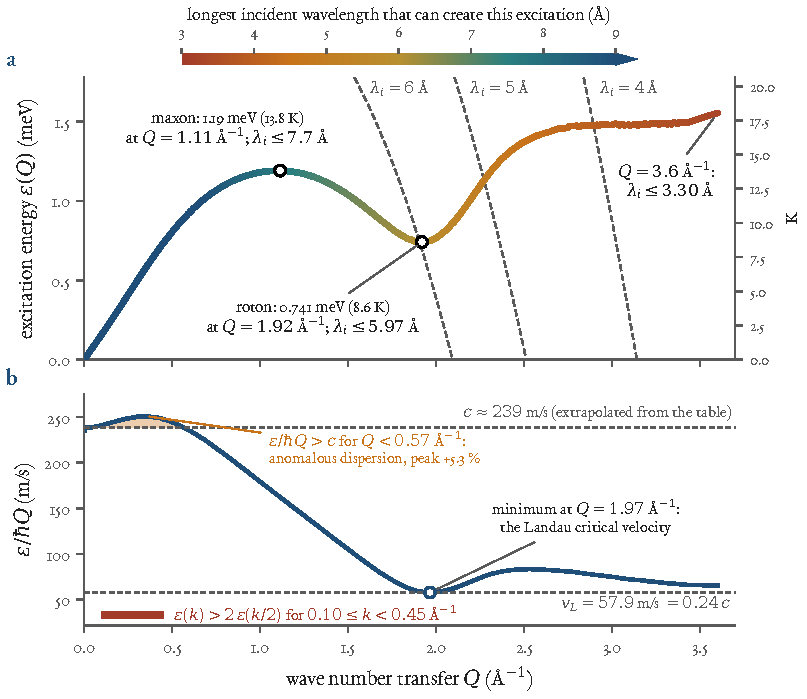
\includegraphics[width=\linewidth]{figures/ch01_bench.pdf}
\caption[The curve the neutron has to find]{The curve the neutron has to find. \textbf{(a)}~Dispersion relation of superfluid $^4$He at saturated vapour pressure, from the table of \cite{Godfrin2021} (author-processed values, not raw counts; open circles: maximum and minimum of the table). The \emph{colour is not data}: it is the longest incident wavelength with which a neutron could create the excitation at that point, from inequality \eqref{ch01:eq-vmin} (statement 5 of \cref{ch01:sec-proof}); a point above a dashed line, the kinematic limit of a neutron of wavelength $\lambda_i=6$, 5 or 4~\AA, cannot be reached with it. These are limits of kinematics, not instrument settings. \textbf{(b)}~Phase velocity $\varepsilon/\hbar Q$ of the same table; $c$ is extrapolated from $\varepsilon/\hbar Q=c(1+aQ^2)$ fitted on $0<Q\le0.2$~\AA$^{-1}$. Shaded: $\varepsilon/\hbar Q>c$. Red bar: $\varepsilon(k)>2\varepsilon(k/2)$ on a cubic-spline interpolation of the table (below $0.1$~\AA$^{-1}$ the table's rounding, $5\times10^{-5}$~meV, is comparable with the effect). Script: \texttt{figures/ch01\_bench.py}.}
\label{ch01:fig-bench}
\end{figure}

Energy and momentum conservation limit what a given incident wavelength can reach. The three vectors $\mathbf k_i$, $\mathbf k_f$ and $\mathbf Q$ form a triangle, so $|k_i-k_f|\le Q\le k_i+k_f$; together with $E_f=E_i-\varepsilon$ this bounds the energy that can be left in the sample at a wave-vector transfer $Q$,
\[
\varepsilon\;\le\;\frac{\hbar^2}{2m_n}\bigl(2k_iQ-Q^2\bigr)\;=\;E_i-\frac{\hbar^2}{2m_n}(k_i-Q)^2 ,
\]
a downward parabola with its apex $E_i$ at $Q=k_i$: the dashed lines of the figure. Solved for the neutron instead of the sample, the same inequality reads $k_i\ge Q/2+m_n\varepsilon/\hbar^2Q$, or, multiplied by $\hbar/m_n$,
\begin{equation}
v_n\;\ge\;\frac{\hbar Q}{2m_n}\;+\;\frac{\varepsilon}{\hbar Q}.
\label{ch01:eq-vmin}
\end{equation}
The first term is the speed at which a neutron can just deliver the wave-vector transfer $Q$ by reversing its direction without losing energy; the second is the price of the energy $\varepsilon$ paid at that wave number, the phase velocity of the excitation. \Cref{ch01:sec-proof} gives this inequality in Lean; it is what colours the curve of \cref{ch01:fig-bench}(a). To create the roton a neutron must be at least as fast as 663~m/s, that is $\lambda_i\le5.97$~\AA\ (and $E_i\ge2.30$~meV); to reach the last row of the table, $Q=3.6$~\AA$^{-1}$, it must have $\lambda_i\le3.30$~\AA; to reach $Q=3$~\AA$^{-1}$, $\lambda_i\le3.88$~\AA. At the other end, as $Q\to0$ the condition becomes $v_n\ge c$: the neutron must outrun sound, $\lambda_i\le16.6$~\AA. For comparison, the ILL lists the incident wavelengths of IN5 as $1.8$ to 20~\AA\ \cite{ILLIN5}, a range that contains all of these; what was set for which part of the curve in the 2021 measurement is not something this book describes.

Panel (b) of the figure divides the table by $Q$. The phase velocity $\varepsilon/\hbar Q$ tends at small $Q$ to the speed of sound, which the extrapolation puts at 239~m/s. It then \emph{rises}, by 5.3 per cent to 251~m/s at $Q=0.35$~\AA$^{-1}$, falls back through $c$ at $0.57$~\AA$^{-1}$, and goes on down to a minimum of 57.9~m/s, $0.24\,c$, at $Q=1.97$~\AA$^{-1}$, beside the roton. The rise is the \emph{anomalous dispersion} of helium-4 at low pressure, and its consequence is kinematic: a phonon may then decay into two (\cref{ch01:sec-proof}). The minimum is the Landau critical velocity: an object moving through the fluid at a speed below it cannot create any excitation, because creating one of wave number $Q$ and energy $\varepsilon$ takes a speed of at least $\varepsilon/\hbar Q$ --- the very quantity that appears as the second term of \eqref{ch01:eq-vmin}, seen from the other side. Real flows lose their superfluidity earlier, typically by nucleating vortices \cite{Donnelly1991}, so $v_L$ is the bound of an idealized argument and not a measured threshold.

%% ------------------------------------------------------------------------------------------------------------------------
\section{From the curve to the calorimeter}\label{ch01:sec-chain}

The second paper does more than tabulate a curve. It follows Landau's chain from the dispersion relation to the thermodynamics, and the chain is short enough to write down.

\begin{keybox}[Landau's chain, from $\varepsilon(k)$ to $C_V$]
At temperature $T$ the fluid is a gas of bosonic excitations, so its energy per volume $V$ and its specific heat are
\[
\frac{E}{V}=\int\!\frac{\dd^3k}{(2\pi)^3}\,\frac{\varepsilon(k)}{e^{\varepsilon(k)/k_BT}-1},\qquad C_V=\frac{\partial E}{\partial T}.
\]
For phonons, $\varepsilon=\hbar ck$, the integral is the Bose integral $\int_0^\infty t^3/(e^t-1)\,\dd t=\pi^4/15$ and
\[
C_V=A\,T^3,\qquad A=\frac{2\pi^2k_B^4V}{15\,\hbar^3c^3},
\]
the $T^3$ law. A correction $\alpha_nk^n$ to the dispersion changes the density of states $k^2\,\dd k/\dd\varepsilon$ and with it the coefficient of the next power of $T$; for $\varepsilon=\hbar ck(1+\alpha_2k^2+\dots+\alpha_6k^6)$ the result is the series of Eq.~(22) of the paper, $C_V=AT^3+CT^5+DT^6+ET^7+KT^8+LT^9$, with no $T^4$ term because $\alpha_1=0$. Four of the six coefficients ($A$, $C$, $E$, $L$) bring the even zeta values $\zeta(4)$, $\zeta(6)$, $\zeta(8)$, $\zeta(10)$, which are rational multiples of powers of $\pi$; the other two bring $\zeta(7)$ and $\zeta(9)$, which have no known closed form, and this is why a zeta value is written out in $D$ and $K$ and in no other coefficient.
\end{keybox}

A six-term series whose coefficients are built from products of the $\alpha_n$ and from zeta values is not something a reader can re-derive on a train, and the paper itself remarks that earlier published versions of this series contain errors. A measured curve cannot check an algebraic identity, and a calorimeter cannot either: the series is a mathematical consequence of the model dispersion, and a mathematical consequence is what a proof assistant can certify. \Cref{ch01:sec-proof} says what was certified, and \cref{ch04} follows the whole chain. Which of the series' truncations describes the measured curve at a given temperature is a different question, about a measured function; it is not a theorem and the proof assistant does not touch it.

%% ------------------------------------------------------------------------------------------------------------------------
\section{Three instruments, one discipline}\label{ch01:sec-method}

Each instrument is blind where another sees (\cref{ch01:tab-instruments}). A measurement says nothing about whether a printed coefficient is algebraically right, and a calorimeter cannot find a misprinted exponent. A proof says nothing about helium: it holds for every model that satisfies its hypotheses, and whether helium does is not a mathematical question. A simulation shows what a model does and can be wrong in ways that conservation laws catch, but it cannot say \emph{why}, and it cannot tell a theorem from a coincidence.

\begin{table}[t]\centering\small
\renewcommand{\arraystretch}{1.28}
\begin{tabularx}{\linewidth}{@{}>{\bfseries\raggedright\arraybackslash}p{1.65cm}>{\raggedright\arraybackslash}X>{\raggedright\arraybackslash}X>{\raggedright\arraybackslash}X@{}}
\toprule
 & can establish & cannot establish & a case from this programme \\
\midrule
The bench & a number about nature, with its error bar and the procedure that produced it & that a printed formula is algebraically right; why the number is what it is & a six-term specific-heat series whose predecessors in the literature contained errors (\cref{ch01:sec-chain}) \\
The proof & that a statement follows from its hypotheses for all values, without arithmetic slips & that the hypotheses describe helium; that a correct theorem is new & the `dual length' theorem about the Bogoliubov spectrum: correct, and withdrawn as a finding on 2026-09-20 \\
The solver & what a model does for given parameters, with conservation laws as a check & why; that a coincidence is not a theorem; that the model is nature & a vortex pair that moved 23 per cent faster than the point-vortex formula on a torus, until the proof explained why (\cref{ch01:sec-solver}) \\
\bottomrule
\end{tabularx}
\caption{What each instrument can and cannot establish, with one case of each from the programme behind this book.}
\label{ch01:tab-instruments}
\end{table}

Used together they check one another only if their roles are kept apart, and this book keeps four rules. A theorem is never presented as a measurement, nor a simulation as one. Every statement says which instrument supports it. An analogy between two systems is not a result: before a finding is carried over we name the property it depends on and check that the other system has it (the programme calls this rule LL-15, after the lesson in which it was learned). And failures are published. Three of them concern this chapter.

The `dual length' $\varepsilon^2/(\hbar^2c^2k^3)$ of the Bogoliubov spectrum had a correct Lean proof and was first presented as a finding. A literature check on 2026-09-20 showed it to be a repackaging of known relations whose bound is dimensionally forced and, outside a narrow window of wave numbers, weaker than Onsager's inequality; it was withdrawn (\texttt{RETRACTIONS.md}, R2). A proof assistant could not have told us that, and a literature search did. Second, the pair speed of \cref{ch01:sec-solver} was at first read, in a forked analysis session, as an imprint transient; it is the mean flow that a periodic box forces on a pair (ledger CLAIM-082). A simulation reported the excess faithfully and could not explain it; the explanation came from the theorem of \cref{ch01:sec-proof}. Third, a proposal to certify the zero-sound parameters of two-dimensional helium-3 stopped at the literature gate, before any code, because the numbers it needed were not to be found in open sources (ledger CLAIM-030 and 031); \cref{ch01:sec-handover} comes back to it. In each case what mattered was less the instrument than the mechanism that was in place before the claim was tested.

%% ------------------------------------------------------------------------------------------------------------------------
\section{What the proof assistant says: five statements}\label{ch01:sec-proof}

Lean~4 is a programming language and a proof assistant: a statement written in it is accepted only if a small kernel has checked a complete proof of it \cite{deMoura2021}. The library \texttt{QuantumFluids} \cite{Callens2026lib} collects such statements about quantum fluids on top of Mathlib \cite{Mathlib2020}; at the time of writing it indexes 310 theorems. \Cref{ch02} is the primer. Here are five statements, chosen so that each touches something in this chapter. Each box gives the statement exactly as it stands in the library, or, for the last, in the new file written for this book; the paragraph after it says in words what it asserts and what it does not.

\begin{leanbox}[title={Lean 4 \enspace Statement 1 \enspace BoseIntegral}]{BoseIntegral}
\begin{lstlisting}[style=lean]
noncomputable def debyeEnergy (V kB hbar c I T : ℝ) : ℝ :=
  V / (2 * π ^ 2) * (kB * T) ^ 4 / (hbar * c) ^ 3 * I

theorem debye_specific_heat (V kB hbar c T : ℝ) :
    HasDerivAt (fun T => debyeEnergy V kB hbar c (π ^ 4 / 15) T)
      (2 * π ^ 2 * kB ^ 4 * V / (15 * c ^ 3 * hbar ^ 3) * T ^ 3) T
\end{lstlisting}
\end{leanbox}
\textbf{Statement 1, the leading term of Eq.~(22).} With the Bose integral set to $I=\pi^4/15$, the phonon energy of a volume $V$ has the temperature derivative $2\pi^2k_B^4V\,T^3/(15\,c^3\hbar^3)$: the coefficient $A$ of Eq.~(22), exactly. The value of the integral is the theorem \Lthm{BoseIntegral}{mellin_bose_four}, $\int_0^\infty t^3/(e^t-1)\,\dd t=\pi^4/15$, which Mathlib did not have and which the library derives from the Mellin transform. The theorem \Lthm{PhononSpecificHeat}{phonon_specific_heat} assembles all six terms; the printed coefficients $A,C,D,E,K,L$ and the printed inverse series were derived independently by computer algebra and then proved. The result is a confirmation of the paper, and the programme records it as nothing more: no discrepancy was found. What is not proved is as important: that the coefficients typed into the capstone are the coefficients of the density-of-states polynomial proved in \texttt{PhononSeries} is checked by inspection, not by a theorem, and that the truncated series approximates the specific heat computed from the measured curve is a statement about a measured function.

\begin{leanbox}[title={Lean 4 \enspace Statement 2 \enspace HeliumKinematics}]{HeliumKinematics}
\begin{lstlisting}[style=lean]
def phononDisp (c a k : ℝ) : ℝ := c * k * (1 + a * k ^ 2)

theorem three_phonon_open_iff {c a k₁ k₂ : ℝ} (hc : 0 < c) (h₁ : 0 < k₁) (h₂ : 0 < k₂) :
    phononDisp c a k₁ + phononDisp c a k₂ ≤ phononDisp c a (k₁ + k₂) ↔ 0 ≤ a
\end{lstlisting}
\end{leanbox}
\textbf{Statement 2, when a phonon can decay.} A phonon of wave number $k_1+k_2$ can decay into two collinear phonons of wave numbers $k_1$ and $k_2$, conserving energy and momentum, only if $\varepsilon(k_1)+\varepsilon(k_2)\le\varepsilon(k_1+k_2)$. For the model dispersion $\varepsilon=ck(1+ak^2)$ with $c>0$ this holds exactly when $a\ge0$: the dispersion must bend upward. It is one of the kinematic statements in the analysis of the neutron data of the 2021 paper that the module \texttt{HeliumKinematics} formalizes, and the proof is of the mathematical statement, not of the experiment. \Cref{ch01:fig-bench}(b) is where it meets the measurement: the table's phase velocity exceeds $c$ at small $Q$, and the symmetric split $\varepsilon(k)\ge2\varepsilon(k/2)$ holds on the table for $0.10\le k<0.45$~\AA$^{-1}$. The theorem says nothing about the table beyond the cubic model, and nothing about decay rates.

\begin{leanbox}[title={Lean 4 \enspace Statement 3 \enspace ZeroSound}]{ZeroSound}
\begin{lstlisting}[style=lean]
theorem zero_sound_2d_iff (F : ℝ) :
    (∃ s, 1 < s ∧ 1 + F * (1 - s / √(s ^ 2 - 1)) = 0) ↔ 0 < F
\end{lstlisting}
\end{leanbox}
\textbf{Statement 3, zero sound in two dimensions.} Landau's collisionless kinetic equation for a Fermi liquid with a single Landau parameter $F$ has, in two dimensions, a collective mode with phase velocity $s\,v_F$ when $1+F\bigl(1-s/\sqrt{s^2-1}\bigr)=0$. The mode is undamped when $s>1$, outside the particle--hole continuum. The theorem says that such a root exists if and only if $F>0$; the proof exhibits it, $s=(1+F)/\sqrt{1+2F}$. This is textbook physics \cite{BaymPethick1991}; what is new is only that it is machine-checked. The two-dimensional case is in the library \emph{because} the 2012 measurement is on a two-dimensional film, where the logarithmic three-dimensional formula does not apply. It is not a statement about that film: nothing is claimed about the value of $F$ for it, about the roton-like minimum, or about the damped branch $s<1$ (\cref{ch08}).

\begin{leanbox}[title={Lean 4 \enspace Statement 4 \enspace VortexWinding}]{VortexWinding}
\begin{lstlisting}[style=lean,basicstyle=\ttfamily\footnotesize]
noncomputable def pdiff (a b : ℝ) : ℝ := toIocMod two_pi_pos (-π) (b - a)

theorem loop_sum_eq_mul (θ : ℕ → ℝ) (n : ℕ) (hclosed : θ n = θ 0) :
    ∃ m : ℤ, ∑ i ∈ Finset.range n, pdiff (θ i) (θ (i + 1)) = (m : ℝ) * (2 * π) := by
  refine ⟨- ∑ i ∈ Finset.range n, toIocDiv two_pi_pos (-π) (θ (i + 1) - θ i), ?_⟩
  have h : ∀ i, pdiff (θ i) (θ (i + 1))
      = (θ (i + 1) - θ i)
        - ((toIocDiv two_pi_pos (-π) (θ (i + 1) - θ i) : ℤ) : ℝ) * (2 * π) := by
    intro i; rw [pdiff_eq, zsmul_eq_mul]
  simp_rw [h]
  rw [Finset.sum_sub_distrib, Finset.sum_range_sub (fun i => θ i), hclosed, ← Finset.sum_mul]
  push_cast
  ring
\end{lstlisting}
\end{leanbox}
\textbf{Statement 4, why a computed winding number is an integer.} Here $\theta_i$ are the phases of a field at the points of a closed loop, and \texttt{pdiff} is the principal value in $(-\pi,\pi]$ of a phase step. The theorem says that the sum of the principal steps around a closed loop is an integer multiple of $2\pi$. The proof, shown in full, is one idea: each principal step differs from the plain difference of the phases by a multiple of $2\pi$ (\Lthm{VortexWinding}{pdiff_eq}), and the plain differences telescope to $\theta_n-\theta_0=0$ because the loop is closed. This is why a numerically computed winding number is an integer and not a decimal: the standard phase-winding vortex detector of Gross--Pitaevskii codes relies on it. Multiplied by $\hbar/m$ it gives \Lthm{QuantizedCirculation}{circulation_quantized}: the circulation around a closed loop of sample points is an integer multiple of the quantum $\kappa=h/m$. The same module states exactly when the standard algorithm fails: if a phase step is exactly $\pi$, the two orientations of an edge contribute $2\pi$ instead of cancelling (\Lthm{VortexWinding}{pdiff_add_rev_eq_two_pi_iff}). Not proved: that the integer is the topological charge of the continuum field the samples came from; that is a statement about sampling, and the library's \texttt{ContinuumWinding} module addresses it for continuous loops.

\begin{leanbox}[title={Lean 4 \enspace Statement 5 \enspace NeutronWindow (new in this book)}]{NeutronWindow}
\begin{lstlisting}[style=lean,basicstyle=\ttfamily\footnotesize]
variable {V : Type*} [NormedAddCommGroup V]

noncomputable def energy (hbar m : ℝ) (k : V) : ℝ := hbar ^ 2 * ‖k‖ ^ 2 / (2 * m)

theorem min_incident_wavevector (hbar m : ℝ) (hbar0 : 0 < hbar) (hm : 0 < m) (ki kf : V) (hQ : 0 < ‖ki - kf‖) :
    ‖ki - kf‖ / 2 + m * (energy hbar m ki - energy hbar m kf) / (hbar ^ 2 * ‖ki - kf‖) ≤ ‖ki‖
\end{lstlisting}
\end{leanbox}
\textbf{Statement 5, what a neutron can reach.} This is inequality \eqref{ch01:eq-vmin}. For a neutron that leaves a sample with wave vector $\mathbf k_f$ after arriving with $\mathbf k_i$, and has given the sample the energy $E_i-E_f$ at the wave-vector transfer $Q=\|\mathbf k_i-\mathbf k_f\|>0$, the incident wave number is at least $Q/2+m(E_i-E_f)/\hbar^2Q$. It was written for this book, in the file \texttt{book/lean/Ch01\_NeutronWindow.lean}, together with the two lemmas it rests on, the triangle inequality for $\mathbf Q$ and the parabola bound on the energy transfer; it compiles against the pinned Mathlib with no error and no \texttt{sorry}, its three theorems depend only on the standard axioms \texttt{propext}, \texttt{Classical.choice} and \texttt{Quot.sound}, and two altered statements (the bound raised by $1/10$, or the recoil term $Q/2$ replaced by $Q$) are rejected by the same proof, as they must be. The proof is the reverse triangle inequality and a line of algebra. It is the \emph{necessary} direction only: that every point under the parabola is reachable needs a triangle with three prescribed sides, and that collinear scattering, forward or backward, attains the bound so that it cannot be improved; both are elementary and neither is formalized here. Nothing in it is a statement about an instrument, and nothing is a statement about helium; it is the geometry of a collision, and it is what draws the colour of \cref{ch01:fig-bench}(a).

%% ------------------------------------------------------------------------------------------------------------------------
\section{What the solver shows: one pair, four checks}\label{ch01:sec-solver}

The simplest object that is topological in the sense of statement 4 is a vortex and an antivortex in a two-dimensional superfluid; the cover of this book shows sixteen vortices computed with the same engine. In a model of a Bose condensate by a complex field $\psi(\mathbf r,t)$ the velocity of the fluid is the gradient of the phase, $\mathbf v=(\hbar/m)\nabla\arg\psi$, so that the circulation around a closed loop is $(\hbar/m)$ times the total change of phase, which must be a multiple of $2\pi$: statement 4, again. The vortex is a zero of $\psi$ around which the phase winds by $\pm2\pi$ \cite{Onsager1949,Feynman1955,Gross1961,Pitaevskii1961}. \Cref{ch03} develops the theory; here we only use the object to show the solver at work, and to compare what it reports with what the proof says.

The model is the projected Gross--Pitaevskii equation on a periodic square \cite{Davis2001,Blakie2008},
\[
i\,\partial_t\psi=\mathcal P\Bigl[-\tfrac12\nabla^2\psi+|\psi|^2\psi\Bigr],
\]
with $\mathcal P$ the projector on the Fourier modes below a cutoff, in units $\hbar=m=g=1$ and with background density 1, so that the speed of sound $c=1$ and the healing length $\xi=1$ are the units of speed and length, and $\xi/c$ the unit of time. The engine is the crate \texttt{qf-pgpe} of rusty-SUNDIALS and its Python extension \texttt{qf\_pgpe} \cite{Callens2026sw}; it advances the field by an integrating-factor fourth-order Runge--Kutta scheme, the linear part exactly and the cubic term by RK4, and, as the crate's README reports, its tests integrate the same right-hand side with the CVODE solver as an independent reference (\cref{ch02} introduces the solver itself; CVODE is not used in the computations of this chapter). The box has side $L=64\,\xi$ and $128^2$ points. At $t=0$ a vortex of charge $+1$ is imprinted at $(26,32)$ and an antivortex at $(38,32)$, with the periodic imprint of the engine.

\begin{rustbox}[unbreakable]{a vortex pair in ten time units}
\begin{lstlisting}[style=py,basicstyle=\ttfamily\footnotesize]
import numpy as np, qf_pgpe

s = qf_pgpe.Pgpe(128, 64.0)     # 128^2 points, box 64 xi; g = 1
pos0 = np.array([[26., 32.], [38., 32.]])   # vortex, antivortex
c0 = s.imprint_v2(s.uniform(), pos0, np.array([1, -1]))
c = s.run(c0, 10.0)             # 1000 RK4 steps in one call
for name, f in (("energy", s.energy), ("norm", s.norm)):
    print(f"{name:6s} t=0 {f(c0):.9f}  t=10 {f(c):.9f}  "
          f"relative drift {abs(f(c) - f(c0)) / f(c0):.1e}")
pos, q = s.detect(c)
print("vortices at t=10:", pos.round(3).tolist(), q.tolist())

def winding(psi, loop):         # loop: grid points, first = last
    th = np.angle([psi[i, j] for i, j in loop])
    d = np.diff(th)
    d -= 2 * np.pi * np.ceil((d - np.pi) / (2 * np.pi))   # pdiff
    return d.sum() / (2 * np.pi), np.abs(d).max()

def ring(i0, j0, h):             # ccw square, half-side h
    up = [(i0 + h, j0 + t) for t in range(-h, h)]
    left = [(i0 + h - t, j0 + h) for t in range(2 * h)]
    down = [(i0 - h, j0 + h - t) for t in range(2 * h)]
    right = [(i0 - h + t, j0 - h) for t in range(2 * h)]
    return up + left + down + right + [(i0 + h, j0 - h)]

psi = np.asarray(s.psi(c))
cases = {"around the vortex": pos[0],
         "around the antivortex": pos[1],
         "empty fluid": (47., 40.)}
for name, centre in cases.items():
    i0, j0 = (int(round(x / 0.5)) for x in centre)
    w, step = winding(psi, ring(i0, j0, 7))
    print(f"{name:22s} winding {w:+.15f}  max step {step:.3f}")
\end{lstlisting}
Output of this box, run as it stands (wall-clock time 9.4~s, of which 5.0~s of CPU, on a shared 8-core machine with a load average of 18.5; phase steps in radians):
\begin{lstlisting}[style=plainmono,basicstyle=\ttfamily\footnotesize]
energy t=0 2069.113131399  t=10 2069.113131436  relative drift 1.8e-11
norm   t=0 4096.000000000  t=10 4096.000000033  relative drift 8.0e-12
vortices at t=10: [[26.123, 32.902], [37.877, 32.902]] [1, -1]
around the vortex      winding +1.000000000000000  max step 0.216
around the antivortex  winding -1.000000000000000  max step 0.216
empty fluid            winding +0.000000000000000  max step 0.030
\end{lstlisting}
\end{rustbox}

\Cref{ch01:fig-triptych} shows the field at $t=10$ three ways.

\begin{figure}[!tp]\centering
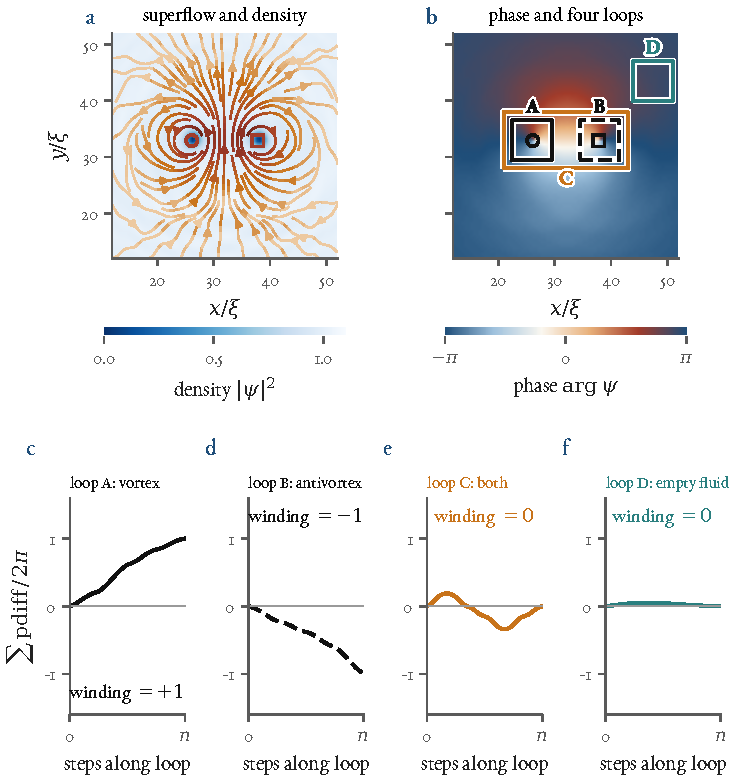
\includegraphics[width=\linewidth]{figures/ch01_triptych.pdf}
\caption[One vortex pair seen by the solver and the proof]{One vortex pair seen by the solver and the proof. \textbf{(a)}~Density (colour) and superflow (streamlines, darker $=$ faster) of the field at $t=10$; the cores of the vortex (circle) and of the antivortex (square) are the two dark dots, $11.75\,\xi$ apart. \textbf{(b)}~Phase $\arg\psi$ and four closed lattice loops: A around the vortex, B around the antivortex, C around both, D in empty fluid. \textbf{(c--f)}~Running sum of the principal phase differences (\texttt{pdiff}) along each loop, in units of $2\pi$: it ends at $+1$, $-1$, $0$, $0$. Engine: \texttt{qf\_pgpe}, $128^2$ points, $L=64\,\xi$, $t=10$. Script: \texttt{figures/ch01\_triptych.py}.}
\label{ch01:fig-triptych}
\end{figure}

\paragraph{Check 1: the proof meets the field.} The sums of principal phase differences around the loops A, B, C and D, in units of $2\pi$, come out as $+1$, $-1$, $0$ and $0$, integers to within $1.4\times10^{-16}$ (the double-precision rounding of the sums; the box above prints them to fifteen decimals), as statement 4 says they must. The theorem fails only if a phase step reaches exactly $\pi$; the largest step along any of the loops of the figure is 0.216~rad, $0.07\,\pi$.

\paragraph{Check 2: the continuum.} The integer of the proof is the sum of \emph{sampled} phases. The circulation of the velocity field itself is another thing, and the one that physics is about. Integrated along the same four loops by Gauss--Legendre quadrature on the exact band-limited field of the engine, $\oint\mathbf v\cdot\mathrm d\mathbf l/\kappa$ is $+1.000000000000$, $-1.000000000000$, $-5.30\times10^{-17}$ and $-1.44\times10^{-17}$, with $\kappa=2\pi\hbar/m$. (A trapezoid rule on the grid values gives 0.9966, 0.9977, 0.9987 and 0.9994 for loops around the vortex of half-side 2, 2.5, 3.5 and 4.5~$\xi$, the deficit shrinking as the loop grows, as a quadrature error of the grid should; the exact integral does not depend on the loop.) In this instance the sampled loop sum is the continuum circulation: the statement that \texttt{QuantizedCirculation} leaves to sampling holds here, to rounding error.

\paragraph{Check 3: the conservation laws.} Over the ten time units of the box above the relative drift of the energy is $1.8\times10^{-11}$, of the norm $8.0\times10^{-12}$ and of the momentum $2.0\times10^{-11}$; over the sixty time units of the next check, $8.6\times10^{-11}$, $4.3\times10^{-11}$ and $5.5\times10^{-11}$. They are the first numbers to look at when one asks whether the engine integrates the model it claims to integrate; they are necessary checks, not sufficient ones (the order of the scheme is tested against CVODE in the crate).

\paragraph{Check 4: the speed of the pair, and what the proof explains.} A pair of opposite vortices at a distance $d$ in the plane moves at $1/d$ (in these units) perpendicular to the line joining them. In a periodic box the periodic images of the two vortices lower this speed, and the standard formula for point vortices on a torus, the Weiss--McWilliams sum \cite{WeissMcWilliams1991}, includes them. We tracked the cores for 60 time units, each time unit, and fitted the displacement of their midpoint on $t\ge20$, after the imprint has relaxed. The measured speed is 0.0932 (fits that start at $t=10$, 20 and 30 give 0.0936, 0.0932 and 0.0928, a half-range of 0.4 per cent, which we take as the uncertainty), against 0.0850 for the planar formula at the mean separation $d=11.76\,\xi$ (standard deviation over the window 0.02) and 0.0757 for the torus formula: 23 per cent more than the point-vortex prediction.

\begin{figure}[!t]\centering
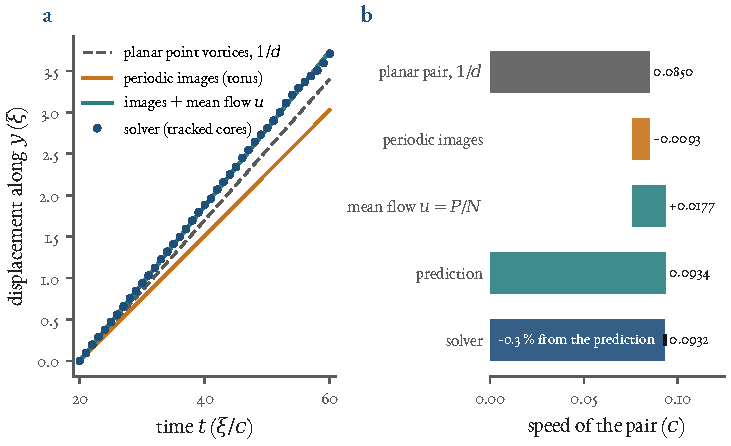
\includegraphics[width=\linewidth]{figures/ch01_budget.pdf}
\caption[Where the speed of the pair comes from]{Where the speed of the pair comes from. \textbf{(a)}~Displacement of the midpoint of the two cores along $y$ from $t=20$, tracked each time unit in the solver (dots), against the planar formula $1/d$, the formula for point vortices on a torus (periodic images), and the torus formula plus the mean flow $u=P/N$ of the whole fluid. \textbf{(b)}~The same as a budget of the speed in units of $c$: planar pair, correction of the periodic images, mean flow, the resulting prediction, and the solver. Script: \texttt{figures/ch01\_budget.py}.}
\label{ch01:fig-budget}
\end{figure}

The missing piece is not in the point-vortex formula. A pair carries the momentum $P\approx2\pi d$ (per unit density, in these units), and in a periodic box that momentum cannot go anywhere: the whole fluid moves, with the mean velocity $u=P/N$ ($N$ the norm), which the formula for point vortices, built on a Green function of zero mean, does not contain. Adding the measured $u=0.0177$ gives 0.0934, within 0.3 per cent of what the solver does, which is inside the spread of the fits (\cref{ch01:fig-budget}).

The proof says that this mean flow is not an accident of the imprint. The phase of $\psi$ must be single-valued, so by statement 4 the circulation around each of the two non-contractible cycles of the torus is $2\pi$ times an integer. Around a vertical cycle at a position $x$ between the vortices the integer differs by one from its value outside, because the circulation around a single core is $2\pi$; so the average of $v_y$ over the box is $(2\pi/L^2)\bigl(n_{\rm in}d+n_{\rm out}(L-d)\bigr)$ with $n_{\rm in}-n_{\rm out}=\pm1$, and its smallest magnitude is $2\pi d/L^2$. The mean of the superfluid velocity of a neutral pair on a torus cannot be made zero. We checked the integers on the field at $t=10$, by exact line integrals around the cycles, in units of $2\pi$: $+1$ along the vertical cycle between the cores, $0$ and $0$ along the two vertical cycles outside them, $0$ and $0$ along the two horizontal ones, each within $5.2\times10^{-14}$ of the integer. They give $u=2\pi\,11.75/L^2=0.0180$, while the momentum of the field gives 0.0177, the difference, 1.6 per cent, being the average of $(1-n)\,v_y$ over the box: the density $n$ is not uniform (it falls to 0.016 at the cores and carries sound waves), so the density-weighted and the plain mean velocities differ. The programme's own $T=0$ sweep over pair sizes shows the same thing at every size \cite{Callens2026a}: the ratio of the measured speed to the torus formula grows in the box frame from 1.06 at $d=6\,\xi$ to 1.49 at $d=16\,\xi$ (the paper's table; \cref{ch07} compares it with the saved file of the sweep), and is 1.004 to 1.005 for $d=8$ to $16\,\xi$ once the mean flow is subtracted. That subtraction is the correction of the early reading of the excess as an imprint transient, mentioned in \cref{ch01:sec-method} (ledger CLAIM-082).

A last honest line. The measured speed is $-0.3$ per cent from the prediction, which is inside the spread of the fits: no residual is resolved. A pair of finite size is a solitary wave of a compressible field (the Jones--Roberts family \cite{JonesRoberts1982}) and its speed departs from the point-vortex value by a correction of the order of $(\xi/d)^2$; the programme measured that correction at $T=0$, with longer runs, as $+0.4$ per cent for $d\ge8\,\xi$ and larger for tighter pairs, which is as large as our uncertainty, so we neither see it nor exclude it. The run took 181~s of wall-clock time on a shared 8-core machine whose load average was 20.2 at its end; the figure is not a benchmark.

%% ------------------------------------------------------------------------------------------------------------------------
\section{What the measurements hand to theory}\label{ch01:sec-handover}

The two measurements hand three things to anyone who works on quantum fluids.

\textbf{A curve.} The dispersion relation of helium-4 from phonon to roton is a table, and a table can be put in front of any theory of the liquid. This book does not compute helium. What the library does is to make explicit which mathematical statements stand between that table and the thermodynamic functions: the Bose integral and the zeta values, the inversion of the dispersion series, the density of states, the kinematics of decay and of the collision itself. Each of them is a place where a printed formula could be wrong without any measurement being able to say which step was at fault.

\textbf{A chain, and the confirmation of one of its links.} Landau's chain from the curve to the calorimeter has a six-term analytic form in the paper, and the form has been derived a second time, independently, and proved. A confirmation is a small thing and the programme records it as small. It is, however, the kind of thing an experimentalist can use: a series that enters an analysis is now one whose algebra is certified, so that a disagreement with a calorimeter, should one appear, is a disagreement about the model and not about the arithmetic.

\textbf{A film, and a question.} The two-dimensional helium-3 film has a collective mode that lives long and has a roton-like minimum. Statement 3 of \cref{ch01:sec-proof} is the part of the story that is a theorem: in Landau's single-parameter description an undamped zero sound exists in two dimensions if and only if $F>0$. To use it on the film one needs the Landau parameters of the film, and the programme did not find an open numerical table of them; it stopped twice, at the literature gate, rather than put a number into the theorem that it could not source. That is not a result about the film, and the roton-like minimum, which lies at a wave number where a single Landau parameter is not the right tool, is outside what the theorem says. It is a map of what is missing.

How can a companion made of proofs and simulations honour a measurement without speaking for the people who made it? We have tried to follow five rules, and they are offered as a standard against which the book can be judged.
\begin{itemize}
\item \emph{Say precisely which statement is used.} Where the library formalizes a statement of a paper, the book names the equation and says whether what was proved is the mathematics of the statement or something about the experiment. It is always the former.
\item \emph{Prove mathematics, not physics.} A theorem of this book is about a model, or about arithmetic, or about the geometry of a collision. It is never a statement about helium.
\item \emph{Leave the measurement its authority.} The only measured curve in this chapter is the authors' table. Our additions to it are kinematics and arithmetic, and they are labelled as such in the figure.
\item \emph{Be useful to the reader of the paper.} The right test of a companion is whether an experimentalist who reads the paper would rather have it than not: a certified series, a stated failure condition of a standard algorithm, a picture of what a neutron can reach.
\item \emph{Put the failures next to the successes.} A tribute that hid its retractions would be a poor one to a craft whose first rule is to report the error bar.
\end{itemize}
The book makes no claim about the data behind the two papers beyond the table described above, and none about the published version of the 2021 paper beyond its Eq.~(22). It has not been reviewed by the people whose measurements it describes.

\begin{honestbox}
\textbf{Proved} (Lean 4.34.0-rc2, Mathlib v4.34.0-rc2, standard axioms): the five statements of \cref{ch01:sec-proof}; the first four belong to the library \texttt{QuantumFluids}, the fifth is new and lives in \texttt{book/lean/Ch01\_NeutronWindow.lean}. They are theorems about a Debye-type energy, about a cubic model dispersion, about Landau's single-parameter kinetic equation, about sums of principal phase differences and about the triangle of a collision; none is a statement about helium or about an instrument. What is not proved: the link between the density-of-states polynomial and the coefficients typed into \Lthm{PhononSpecificHeat}{phonon_specific_heat} (by inspection), the validity of the series for the measured curve, the reachability of points under the neutron parabola, and that a sampled winding is the continuum charge in general.
\par\smallskip\noindent\textbf{Measured}: nothing new. The curve of \cref{ch01:fig-bench} is the authors' processed table; the speed of sound $c\approx239$~m/s is our extrapolation of it, and $v_L$, the phonon excess and the kinematic limits are arithmetic on it. They are not the settings of any experiment.
\par\smallskip\noindent\textbf{Simulated}: one vortex pair in a periodic box of a classical-field model. It reproduces the integer windings, the quantum of circulation and the conservation laws, and moves at the speed predicted from the torus formula plus the mean flow to 0.3 per cent; the residual is not decomposed.
\par\smallskip\noindent\textbf{Only an analogy}: that the pair of a Bose-condensate model says anything about a vortex in helium-4 or in a Fermi liquid. The model has no roton and no Fermi statistics. The mean flow of a periodic box is a property of the box, not of helium. The theorem on zero sound is not applied to the 2012 film.
\par\smallskip\noindent\textbf{Failed or corrected} (programme record): the `dual length' claim, withdrawn 2026-09-20; the early reading of the pair-speed excess as an imprint transient, corrected as the mean flow (CLAIM-082); the zero-sound certification proposal, stopped at the literature gate (CLAIM-030, 031).
\end{honestbox}

%% ------------------------------------------------------------------------------------------------------------------------
\section*{Exercises}\addcontentsline{toc}{section}{Exercises}

\paragraph{Exercise 1.} The roton of \cref{ch01:fig-bench} has $Q_0=1.92$~\AA$^{-1}$ and $\varepsilon_0=0.741$~meV. With $\hbar^2/2m_n=2.072$~meV\,\AA$^2$, use \eqref{ch01:eq-vmin} to find the longest wavelength and the least energy of a neutron that can create it. Then find the longest wavelength that reaches $Q=3$~\AA$^{-1}$, where $\varepsilon=1.478$~meV, and explain why the answer for $Q\to0$ does not depend on $Q$. \emph{Hint:} multiply $k_i\ge Q/2+m_n\varepsilon/\hbar^2Q$ by $\hbar/m_n$; for the energy, $E_i=(\hbar^2/2m_n)k_i^2$; as $Q\to0$ the first term of \eqref{ch01:eq-vmin} vanishes.

\paragraph{Exercise 2.} Take the closed loop of four phases $\theta=(0,\pi,0,\pi)$ (so that $\theta_4=\theta_0=0$). Compute the sum of the principal differences. It is an integer multiple of $2\pi$, as the theorem \Lthm{VortexWinding}{loop_sum_eq_mul} requires; which integer? Is it the winding of the smooth loop that the four samples were taken from? Which statement of the same module explains what has happened? \emph{Hint:} $\mathrm{pdiff}(0,\pi)=\pi$ and $\mathrm{pdiff}(\pi,0)=\pi$, because the principal interval is $(-\pi,\pi]$; a sampled loop cannot tell a wind of $4\pi$ from an oscillation, and the failure condition is exactly a step of $\pi$.

\paragraph{Exercise 3.} A neutral vortex pair of separation $d<L/2$ sits in a periodic square of side $L$ (units $\hbar/m=1$, density 1). Show that the average of $v_y$ over the box is $(2\pi/L^2)\bigl(n_{\rm in}d+n_{\rm out}(L-d)\bigr)$, where the integers $n_{\rm in}$ and $n_{\rm out}$ are the windings of the phase along vertical cycles inside and outside the pair and $n_{\rm in}-n_{\rm out}=\pm1$, and that its least magnitude is $2\pi d/L^2$. Evaluate it for $L=64$, $d=11.75$, and say why the speed of the pair in the box differs from the torus point-vortex speed by about that amount. \emph{Hint:} $\oint v_y\,\mathrm dy=2\pi n(x)$ at fixed $x$ by \Lthm{VortexWinding}{loop_sum_eq_mul}; integrate over $x$; the choice $n_{\rm out}=0$ gives the least magnitude since $L-d>d$.

%% ------------------------------------------------------------------------------------------------------------------------
\section*{Notes and further reading}\addcontentsline{toc}{section}{Notes and further reading}

The two measurements are \cite{Godfrin2012} and \cite{Godfrin2021}; for the excitation spectra of quantum fluids in general see the review \cite{GodfrinKrotscheck2022}. Landau's own papers are \cite{Landau1941} for helium-4 and \cite{Landau1957} for the Fermi liquid; Baym and Pethick \cite{BaymPethick1991} treat the latter, Pitaevskii and Stringari \cite{PitaevskiiStringari2016} the Bose condensate, and Donnelly \cite{Donnelly1991} the quantized vortices of helium~II. For neutron scattering, Squires \cite{Squires2012} is the standard introduction and Glyde \cite{Glyde1994} treats helium specifically. SUNDIALS is described in \cite{Hindmarsh2005}, Lean in \cite{deMoura2021}, Mathlib in \cite{Mathlib2020}; the library and the solver of this book are \cite{Callens2026lib} and \cite{Callens2026sw}, and the transport of vortices in the same engine is the subject of \cite{Callens2026a}. The periodic point-vortex velocity used in \cref{ch01:sec-solver} is that of Weiss and McWilliams \cite{WeissMcWilliams1991}, and the compressible solitary pair is due to Jones and Roberts \cite{JonesRoberts1982}. The reference run of Kwon and Shin \cite{KwonShin2026prr,KwonShin2026data}, which the same engine reproduces, is the subject of \cref{ch09}. The records of what failed are in the programme's \texttt{RETRACTIONS.md}, \texttt{LEDGER.md} and \texttt{LL.md}.
}
\IfCh{ch02}{\chapter{Two Languages: Lean 4 and rusty-SUNDIALS}\label{ch02}

\section{Two ways to be wrong}\label{ch02:wrong}

The first run of the registered controls of the programme's solver for the projected Gross--Pitaevskii equation (PGPE), recorded in an amendment dated 22 September 2026, reported that the
total momentum of an isolated, periodic, two-dimensional fluid had changed by $8.54$ in $20$ time units, one per cent of its value, and had done so identically at two
different time steps. Momentum cannot change in such a system, since translating the periodic box leaves the equation unchanged; and a drift that does not depend on the step is not a
fault of the time stepping but of the equation being stepped. The same run, which tests the norm (control K1), the energy (K2), the momentum (K3) and an exact plane-wave solution (K4),
had found the norm conserved to $4.2\times10^{-10}$ and the plane wave reproduced to $7.0\times10^{-10}$: those two controls passed, and neither could have seen the fault. It sat in a sentence of the
programme's own pre-registration, which said that a cutoff at two thirds of the largest wave number makes the cubic term of the equation free of aliasing. That is the rule for a quadratic
nonlinearity \cite{Orszag1971}; for a cubic term the cutoff has to sit at one half. The aliased scheme is not translation invariant, and the momentum control saw it.\footnote{Amendment~A1 of the programme's pre-registration
(\texttt{docs/designs/PGPE\_BKT\_PREREG.md}, 2026-09-22) and the stored first run \texttt{data/generated/pgpe/known\_answers.json}: $N=64$, $L=32$, a random state of energy $3$ per particle,
$t=20$, momentum drift $8.5358$ at $\Delta t=0.005$ and $8.5358$ at $0.01$. The numbers of this paragraph are quoted from those files, not recomputed.}

A different kind of fault is the subject of a remark in the 2021 paper by Godfrin and his co-authors on the dispersion relation of superfluid
helium-4 \cite{Godfrin2021}. Equation~(22) of that paper gives the phonon specific heat as a series,
$C_V=AT^3+CT^5+DT^6+ET^7+KT^8+LT^9$, and the authors note that earlier published versions of the series contain errors.
The neutron measurement fixes the dispersion relation; the step from the dispersion to the series is algebra, and a formula of that length is
exactly where a coefficient or a sign can be wrong without anyone noticing.

\begin{godfrinbox}{A printed series, and a remark about it}
The inelastic neutron-scattering measurement of Godfrin, Beauvois, Sultan, Krotscheck, Dawidowski, F\aa k and Ollivier on superfluid $^4$He
(spectrometer IN5, Institut Laue--Langevin; Phys.\ Rev.\ B \textbf{103}, 104516 (2021)) gives the Landau phonon--maxon--roton dispersion (the authors' published table runs
from $0$ to $3.6\,\text{\AA}^{-1}$) and the thermodynamic consequences. Its Eq.~(22) is the series above, for a dispersion
$\varepsilon=\hbar ck\,(1+\alpha_2k^2+\dots+\alpha_6k^6)$ with $\alpha_1=0$, and the paper remarks that earlier versions of this series contain errors.
The programme re-derived the series independently and proved all six coefficients in Lean. That is a \emph{confirmation of the printed formula},
not a finding, and a proof of a mathematical statement, not of the experiment; \cref{ch04} tells it.
\end{godfrinbox}

The two faults call for two different instruments, and this chapter is a primer on both. The second fault, an algebraic slip, is the business of a
proof assistant: a computer checks the derivation, and a wrong coefficient cannot pass. The first fault is not. The programme had a Lean theorem about the
cubic term, and the theorem was true; it was about the \emph{exact} Galerkin convolution on an additive group such as the integer lattice, while the program evaluated a
different function, a fast Fourier transform on a periodic grid, which coincides with the convolution only when no triple of wave vectors wraps around the
grid. A proof checks a statement against its hypotheses and a simulation checks a program against an expectation; neither checks that the program computes
the object the statement is about.

\begin{keybox}[The division of labour]
A theorem is about a \emph{function}; a run is of a \emph{program}. Lean can establish that the function has a property for every state and every
parameter. The solver can show that the program reproduces an exact solution, an independent integrator or a conservation law to a stated precision, in a stated
case. Each instrument is blind where the other sees, and the instructive cases are those in which they disagree.
\end{keybox}

We follow one equation through both languages. \Cref{ch02:lean} is Lean in twenty minutes; \cref{ch02:theorem} states the theorems that concern the
equation; \cref{ch02:solver} is the solver in twenty minutes; \cref{ch02:known,ch02:planewave,ch02:alias} are three experiments, the last of
which is the fault above, reproduced and measured; \cref{ch02:see} sorts out which instrument can see what.

\section{Lean 4 in twenty minutes}\label{ch02:lean}

Lean~4 \cite{deMoura2021} is at once a programming language and a proof assistant. In it a statement is a \emph{type}, a proof of the statement is a
\emph{term} of that type, and a small program, the \emph{kernel}, checks that the term has the type it is claimed to have. The kernel, together with the axioms
it is told to assume, is what a reader has to trust; the elaborator and the tactics that build terms are not trusted, because whatever they produce is
re-checked. Mathlib \cite{Mathlib2020} is the community library of mathematics on which the programme builds. The programme's own library, \lean{QuantumFluids},
adds 37 modules with 310 theorems and lemmas (413 declarations in all) on the mathematics of quantum fluids, compiled with Lean 4.34.0-rc2 against the matching
Mathlib; its sources are in \texttt{lean\_src/}. Every statement quoted from it in this book is copied from there and cited by module and name.
The Lean written for this chapter is marked \emph{new} in the title of its box, lives in \texttt{book/lean/}, and was compiled with zero errors and no \lean{sorry};
the \lean{\#print axioms} lines quoted below are those of the compiler.

The box below contains the whole vocabulary needed to read a Lean statement.

\begin{leanbox}{new: Ch02\_Primer}
\begin{lstlisting}[style=lean]
#check (2 : ℕ)                  -- 2 : ℕ
#check (2 + 2 = 4)              -- 2 + 2 = 4 : Prop
example : 2 + 2 = 4 := rfl      -- a proof is a term of that type

theorem and_swap' (p q : Prop) (hp : p) (hq : q) : q ∧ p :=
  ⟨hq, hp⟩

theorem two_add_two : (2 : ℝ) + 2 = 4 := by norm_num

theorem one_add_nilpotent_inv {R : Type*} [CommRing R]
    (e : R) (h : e ^ 2 = 0) : (1 + e) * (1 - e) = 1 := by
  linear_combination (-1 : R) * h
\end{lstlisting}
\end{leanbox}

The first two lines ask Lean for the type of an expression: \lean{2} is a natural number, and \lean{2 + 2 = 4} is a proposition, an element of the type \lean{Prop}.
The line \lean{example : 2 + 2 = 4 := rfl} proves it: both sides reduce to the same numeral, so reflexivity of equality is a proof. The theorem \lean{and\_swap'} says
that if two propositions hold then they hold in the other order; its proof is the pair \lean{⟨hq, hp⟩}, a term written by hand. The theorem
\lean{two\_add\_two} is about real numbers, and its proof is a \emph{tactic}: \lean{norm\_num} searches for a proof and hands the result to the kernel.

The last theorem is the pattern the library uses at scale. In any commutative ring \lean{R} with an element \lean{e} satisfying \lean{e \^{} 2 = 0}, the element
\lean{1 + e} has the inverse \lean{1 - e}. The tactic \lean{linear\_combination (-1 : R) * h} is a \emph{certificate}: it asserts that the goal, minus $-1$ times the
hypothesis \lean{h}, is an identity of commutative rings, and \lean{ring} checks that identity. The certificate was supplied from outside and the kernel checks it;
nothing about how it was found has to be believed. The module \lean{PhononSeries} uses exactly this pattern for the series of the previous
section: its certificates, computed by computer algebra, run to several thousand characters per line (see \Lthm{PhononSeries}{kPow2_eq}) and are checked by the
kernel like the toy above. Truncating a power series at order $e^8$ becomes the statement \lean{e \^{} 8 = 0} in a commutative ring, with no analysis needed.

\paragraph{What the kernel refuses.} A checker is only worth having if it can say no. With the coefficient of the certificate mistyped (\lean{(1 : R)} instead of \lean{(-1 : R)}),
the same tactic refuses; and so does \lean{norm\_num} on a false numerical statement. The compiler's reply to the file \texttt{book/lean/Ch02\_NegativeControl.lean}, which exists only to be refused
(file path shortened, and the hygiene mark that Lean prints after \lean{inst} omitted):
\begin{lstlisting}[style=plainmono]
Ch02_NegativeControl.lean:9:2: error: ring failed, ring expressions not equal
R : Type u_1
inst : CommRing R
e : R
h : e ^ 2 = 0
⊢ -(e ^ 2 * 2) = 0
Ch02_NegativeControl.lean:12:29: error: unsolved goals
⊢ False
\end{lstlisting}
The residual $-2e^2$ is the evidence: with the wrong sign the goal minus the certificate is not zero as a ring identity (the goal needed $-e^2$ and the certificate supplied $+e^2$), and no proof
is produced. The second error is \lean{norm\_num} reducing \lean{2 + 2 = 5} to \lean{False}.

\paragraph{What an axiom audit looks like.} A Lean file can end with a line \lean{\#print axioms} for each theorem, which lists the axioms the proof ultimately depends on; the library files carry such lines (written by a script), and Appendix~\ref{appA} tabulates the
audit of every module. The file of the box above prints
\begin{lstlisting}[style=plainmono]
'QuantumFluids.Ch02Primer.and_swap'' does not depend on any axioms
'QuantumFluids.Ch02Primer.two_add_two' depends on axioms: [propext, Classical.choice, Quot.sound]
'QuantumFluids.Ch02Primer.one_add_nilpotent_inv' depends on axioms: [propext, Quot.sound]
\end{lstlisting}
The three names are the standard foundation of classical mathematics in Lean and Mathlib (propositional extensionality, the axiom of choice, soundness of quotients);
\lean{and\_swap'} needs no axiom at all, and the certificate needs two. An incomplete proof shows up as a fourth name, \lean{sorryAx}: when the first draft of this chapter's Lean file
contained a proof that did not compile, the compiler reported the error and replaced the proof by \lean{sorry}, and the audit lines of the two theorems that depended on it read
\lean{[propext, sorryAx, Classical.choice, Quot.sound]}. That line is the reason the audit exists.

\paragraph{A program is not a theorem.} Lean also runs programs. The three commands
\begin{lstlisting}[style=lean]
#eval (List.range 6).map (fun n => n ^ 2)
#eval (0.1 + 0.2 : Float)
#eval ((0.1 + 0.2 : Float) == 0.3)
\end{lstlisting}
print, in that order,
\begin{lstlisting}[style=plainmono]
[0, 1, 4, 9, 16, 25]
0.300000
false
\end{lstlisting}
\lean{Float} is the machine's double-precision number, the same 64-bit format as \texttt{float64} in numpy and \texttt{f64} in Rust, and in it the sum of $0.1$ and $0.2$ is
not $0.3$. In the same file the theorem \lean{(1 / 10 + 2 / 10 : ℝ) = 3 / 10} is proved by \lean{norm\_num}, because in the field of real numbers the equation is exact.
A theorem about \lean{ℝ} is a statement about mathematics; what a program returns is a statement about a finite machine. Nothing in the library speaks about the rounding of
any program, and that is why the solver of this book is checked by experiment and the equation by proof.

\section{A theorem about the equation the solver integrates}\label{ch02:theorem}

The projected Gross--Pitaevskii equation \cite{Davis2001,Blakie2008} is the classical-field description of a Bose fluid used throughout the programme. In units $\hbar=m=1$, on a
periodic box of side $L$,
\begin{equation}\label{ch02:eq-pgpe}
 \ii\,\partial_t\psi \;=\; P\Bigl[-\tfrac12\nabla^2\psi+g\,|\psi|^2\psi\Bigr],
\end{equation}
where $P$ keeps the Fourier modes with $|k|\le k_{\rm cut}$ and discards the others. Writing $\psi(x,t)=\sum_{k\in\Lambda}a_k(t)\,\ee^{\ii k\cdot x}$ with $k=2\pi n/L$, $n\in\mathbb Z^2$, and
$\Lambda$ the finite set of retained modes, the equation becomes a system of ordinary differential equations,
\begin{equation}\label{ch02:eq-modes}
 \ii\,\dot a_k=\omega_k\,a_k+g\,N_k(a),\qquad \omega_k=\tfrac12|k|^2,\qquad
 N_k(a)=\sum_{\substack{k_1,k_2,k_3\in\Lambda\\ k_1+k_3=k+k_2}}a_{k_1}\,\overline{a_{k_2}}\,a_{k_3},
\end{equation}
for $k\in\Lambda$. This is the system that the Lean module \lean{GPGalerkin} is about, with an arbitrary additive group in place of $\mathbb Z^2$ and an arbitrary finite
set $\Lambda$ (nothing in what follows depends on which modes are retained), and with the amplitudes called $\psi_k$ and the integer vectors $n$ as the elements of the group (the factor $2\pi/L$ sits in $\omega$). The box below quotes its definition of $N$ and two of its theorems.

\begin{leanbox}{GPGalerkin}
\begin{lstlisting}[style=lean]
-- variable {G : Type*} [AddCommGroup G] [DecidableEq G]

noncomputable def nl (Λ : Finset G) (ψ : G → ℂ) (k : G) : ℂ :=
  ∑ k1 ∈ Λ, ∑ k2 ∈ Λ, ∑ k3 ∈ Λ,
    if k1 + k3 = k + k2 then ψ k1 * (starRingEnd ℂ) (ψ k2) * ψ k3 else 0

theorem pairing_eq_sum (Λ : Finset G) (ψ : G → ℂ) :
    pairing Λ ψ =
      ∑ q ∈ diffs Λ, dens Λ ψ q * (starRingEnd ℂ) (dens Λ ψ q) := by
  -- (proof abridged) rearrangement of finite sums

theorem mass_rate_zero (Λ : Finset G) (ψ : G → ℂ) (ω : G → ℝ)
    (g : ℝ) :
    ∑ k ∈ Λ,
      ((starRingEnd ℂ) (ψ k) *
        ((ω k : ℂ) * ψ k + (g : ℂ) * nl Λ ψ k)).im = 0 := by
  -- (proof abridged) termwise, conj ψ_k * (ω_k ψ_k + g N_k) is
  -- the real number ω_k |ψ_k|² plus g * (conj ψ_k * N_k); the
  -- second parts sum to g * pairing Λ ψ, whose imaginary part is
  -- 0 (pairing_im_zero): pairing Λ ψ is a sum of squared moduli
\end{lstlisting}
\end{leanbox}

The symbols: \lean{Finset G} is a finite subset of the group \lean{G}; \lean{∑ k ∈ Λ, f k} is the finite sum; \lean{starRingEnd ℂ} is complex conjugation; \lean{.im} is the imaginary part;
\lean{(ω k : ℂ)} is a real number regarded as a complex one. The definition \lean{nl} is the sum of \cref{ch02:eq-modes}, with the condition
$k_1+k_3=k+k_2$ written as an \lean{if}. The theorem \Lthm{GPGalerkin}{pairing_eq_sum} says that the quartic interaction sum $Q=\sum_k\overline{\psi_k}N_k$ equals $\sum_q|A_q|^2$, where
$A_q=\sum_{a-b=q}\psi_a\overline{\psi_b}$ is the Fourier transform of the density $|\psi|^2$; hence $Q$ is real and non-negative (\Lthm{GPGalerkin}{pairing_nonneg}), which
is the defocusing sign of the interaction, for every $\Lambda$. The theorem \Lthm{GPGalerkin}{mass_rate_zero} is the algebraic core of the conservation of the norm: for
$\ii\dot\psi_k=G_k$ one has $\mathrm d|\psi_k|^2/\mathrm dt=2\,\mathrm{Im}(\overline{\psi_k}G_k)$, so the theorem says that the \emph{rate} of change of $\sum_k|\psi_k|^2$ is zero.
The whole conservation law is the statement that a certain sum is real, and the abridged proof says why. (All thirteen theorems of the module depend on the three standard axioms and on nothing else, as the audit lines at the end of the file show.)

What the theorem does not say is as important. It does not say that the system has a solution, or that the solution is unique; it does not say that
$\sum_k|\psi_k|^2$ is constant along a solution (that needs the chain rule, which the library does not formalize); and it says nothing about the numbers that any
integrator returns. The companion statement for the energy, \Lthm{GPGalerkin}{energy_rate_zero}, is of the same kind: an algebraic core, with the same limits, resting on the gradient identity
\Lthm{GPGalerkin}{grad_identity}.

The library has no statement about the third conservation law of this equation, momentum. The programme's pre-registration of the solver (its section~4) said otherwise: it
stated that the invariants of the controls K1 to K3 were theorems of \lean{GPGalerkin} and that the projector did not change them. Two of the three were
there as algebraic cores only, and the third was not there at all. The fault of \cref{ch02:wrong} was in the second half of that sentence. The statements written for this chapter
repair the first half; \cref{ch02:alias} measures the second.

\begin{leanbox}{new: Ch02\_Galerkin}
\begin{lstlisting}[style=lean]
-- variable {G : Type*} [AddCommGroup G] [DecidableEq G]
-- nl : as in GPGalerkin, copied verbatim

noncomputable def planeWave (a₀ : ℂ) (ω t : ℝ) : ℂ :=
  a₀ * Complex.exp (-(Complex.I * ω) * t)

noncomputable def planeState (k0 : G) (a₀ : ℂ) (Ω t : ℝ) :
    G → ℂ :=
  fun x => if x = k0 then planeWave a₀ Ω t else 0

noncomputable def galerkinField (Λ : Finset G) (ω : G → ℝ)
    (g : ℝ) (ψ : G → ℂ) (k : G) : ℂ :=
  -Complex.I * ((ω k : ℂ) * ψ k + (g : ℂ) * nl Λ ψ k)

theorem planeState_solves_galerkin (Λ : Finset G) (k0 : G)
    (hk0 : k0 ∈ Λ) (ω : G → ℝ) (g : ℝ) (a₀ : ℂ) (k : G)
    (t : ℝ) :
    HasDerivAt
      (fun s : ℝ =>
        planeState k0 a₀ (ω k0 + g * ‖a₀‖ ^ 2) s k)
      (galerkinField Λ ω g
        (planeState k0 a₀ (ω k0 + g * ‖a₀‖ ^ 2) t) k) t := by
  -- (proof abridged) nl of a one-mode state is |a|² a on that
  -- mode and 0 elsewhere (nl_single); on the mode, |planeWave|
  -- is constant and planeWave' = -i Ω planeWave
\end{lstlisting}
\end{leanbox}

\paragraph{The exact plane wave.} The box above states the solution on which the programme's fourth known answer (K4) rests.
A single occupied mode $k_0$ with amplitude $a_0\,\ee^{-\ii\Omega t}$, where $\Omega=\omega_{k_0}+g|a_0|^2$, solves the Galerkin system on every finite mode set that contains $k_0$, for
every dispersion $\omega$, every coupling $g$ and every amplitude. The theorem evaluates the vector field of \cref{ch02:eq-modes} on the plane-wave state, component by component, and equates it
to the time derivative of that component. It is a statement about $\mathbb R$ and $\mathbb C$ and about no program; \cref{ch02:planewave} asks three integrators to reproduce it.

\begin{leanbox}{new: Ch02\_Galerkin}
\begin{lstlisting}[style=lean]
theorem momentum_rate_zero (Λ : Finset G) (ψ : G → ℂ)
    (ω : G → ℝ) (g : ℝ) (p : G →+ ℝ) :
    ∑ k ∈ Λ, p k * ((starRingEnd ℂ) (ψ k) *
      ((ω k : ℂ) * ψ k + (g : ℂ) * nl Λ ψ k)).im = 0 := by
  -- (proof abridged) the four-fold sum over (a, b, c, d) with
  -- b + d = a + c of p a * conj ψ_a ψ_b conj ψ_c ψ_d; the
  -- renamings a<->c, b<->d, (a,b,c,d)->(b,a,d,c); additivity:
  -- p a + p c = p (a + c) = p (b + d) = p b + p d; so it is real

theorem no_momentum_on_torus (N : ℕ) [NeZero N]
    (p : (ZMod N × ZMod N) →+ ℝ) (x : ZMod N × ZMod N) :
    p x = 0 := by
  -- (proof abridged) N • x = 0 in the torus, so N * p x = 0 in ℝ
\end{lstlisting}
\end{leanbox}

\paragraph{Momentum, and the hypothesis that carries it.} The box above is the new statement behind the fault of \cref{ch02:wrong}. Here \lean{p : G →+ ℝ} is an \emph{additive map}: $p(k+k')=p(k)+p(k')$.
On $G=\mathbb Z^2$ these are exactly the linear combinations of the two components of the wave vector, so \lean{momentum\_rate\_zero} says that the rate of change of the total momentum
$\sum_k p(k)\,|\psi_k|^2$ vanishes, for every finite $\Lambda$ and every state. The constant weight $p\equiv1$ is not additive (the norm has its own theorem and proof); the momentum theorem uses, besides the resonance condition $k_1+k_3=k+k_2$, \emph{only} that $p$ is additive. The abridged proof is short. The nonlinear part of the momentum rate is
the imaginary part of the four-fold sum $S_a=\sum p(a)\,\overline{\psi_a}\psi_b\overline{\psi_c}\psi_d$ over quadruples with $b+d=a+c$. Renaming $a\leftrightarrow c$ leaves the summand unchanged, so
$S_a=S_c$, and likewise $S_b=S_d$ when the weight is $p(b)$ or $p(d)$; additivity and the resonance condition give $p(a)+p(c)=p(b)+p(d)$, so $S_a+S_c=S_b+S_d$ and therefore $S_a=S_b$; and
complex conjugation maps the summand at $(a,b,c,d)$ to the summand at $(b,a,d,c)$, so $\overline{S_a}=S_b=S_a$. A number equal to its conjugate is real. In the file the three renamings are
three short chains of \lean{Finset.sum\_comm}, and the last step is one \lean{linear\_combination}; a corollary instantiates $G=\mathbb Z\times\mathbb Z$ and $p(k)=k_1$.

The second theorem of the box says why the hypothesis is not decoration. On the periodic grid $\mathbb Z_N\times\mathbb Z_N$, where the engine's wave vectors live, every additive map to the real numbers is
zero: there is no additive momentum, so \lean{momentum\_rate\_zero} has no content there. This does \emph{not} prove that momentum fails to be conserved by a wrapped-around scheme (that is a
measurement, \cref{ch02:alias}); it says that the proof has nothing to stand on. It follows (\lean{no\_additive\_wavenumber} in the file) that the wave number itself, $k\mapsto k$, is not an additive
function modulo $N$, which is the formal form of ``aliasing breaks translation invariance''.

\section{rusty-SUNDIALS in twenty minutes}\label{ch02:solver}

\paragraph{What CVODE does.} CVODE integrates $y'=f(t,y)$, $y(t_0)=y_0$, by linear multistep methods: the new value is built from several previous values and from $f$, with a step $h$ and
an order $q$ that the solver changes as it goes. Two families are offered. The Adams--Moulton methods (orders 1--12) are meant for smooth, non-stiff problems and the backward differentiation formulas
(BDF, orders 1--5) for stiff ones. Both are implicit, the new value appears on both sides, and in the Rust implementation both are solved by the same Newton iteration with a dense LU factorization of
$I-\gamma J$; when the user supplies no Jacobian, as in the Python module, $J$ is built column by column by finite differences, at the price of $n$ extra evaluations of $f$ per Jacobian for a system of
dimension $n$. The solution is kept as a Nordsieck array of scaled derivatives. After each step the solver estimates the local error from the size of the Newton correction,
weights it component by component with $1/(\mathrm{rtol}\,|y_i|+\mathrm{atol})$, accepts or rejects the step, and chooses $h$ and $q$ for the next one. The user states a tolerance, not a step. What the
tolerance controls is the \emph{local} error of each step; the error of the final answer is not guaranteed to be of that size, and \cref{ch02:known} shows how far it can stray.

\paragraph{What rusty-SUNDIALS is.} rusty-SUNDIALS is the programme's Rust implementation of this algorithm, translated, in the words of its source files, from the C code of the SUNDIALS suite \cite{Hindmarsh2005}. The Python
module \texttt{rusty\_sundials} exposes one class, \lean{CvodeSolver(method, rtol, atol, max\_steps)}, with one method, \lean{solve(rhs, t0, y0, t\_out)}, which calls the user's Python function \lean{rhs(t, y)} and
returns the pair $(t,y)$ at the end of the interval and nothing else; a trajectory is obtained by many calls, and every call starts the integration afresh. The Rust source calls the order selection of its BDF path a simple heuristic, so step counts need not match those of the C code, and its repository's README speaks of Lean~4 specifications of the solver that this book
neither uses nor re-checks. Nothing in this book is a proof about the Rust code. It is tested: against closed-form solutions, against a second integrator of the same equation, and against the programme's
numpy implementation of the engine. The word ``verified'' in the title of the software paper \cite{Callens2026sw} is used in that sense: its claims are agreements with reference answers, listed there with their precision.

\begin{rustbox}{CVODE from Python}
% CODE snippet1
\begin{lstlisting}[style=py]
import math
from rusty_sundials import CvodeSolver

calls = 0
def rhs(t, y):
    # x'' = -x written as a first-order system (x, v)
    global calls
    calls += 1
    return [y[1], -y[0]]

T = 20 * math.pi        # ten periods; the exact solution is (cos T, -sin T)
for method in ("adams", "bdf"):
    calls = 0
    # arguments: method, rtol, atol, max_steps
    solver = CvodeSolver(method, 1e-8, 1e-10, 100000)
    t, y = solver.solve(rhs, 0.0, [1.0, 0.0], T)
    err = max(abs(y[0] - math.cos(T)), abs(y[1] + math.sin(T)))
    print(f"{method:5s} rhs calls {calls:6d}  error {err:.2e}")
\end{lstlisting}
% OUTPUT snippet1
\begin{lstlisting}[style=plainmono]
adams rhs calls   1549  error 3.76e-07
bdf   rhs calls   5217  error 2.53e-06
\end{lstlisting}
Output of \texttt{figures/ch02\_snippets.py}, run with the module described below.
\end{rustbox}

The box above is the whole interface in use: ten periods of the harmonic oscillator, both methods, the exact answer known. The number of calls of \lean{rhs}, which includes the columns
of the finite-difference Jacobian, is the \emph{cost} used throughout this chapter; unlike wall time it does not depend on the load of a shared machine. Both runs asked for a relative tolerance of $10^{-8}$,
and neither delivered a final error of that size: $3.8\times10^{-7}$ and $2.5\times10^{-6}$.

\paragraph{A defect, and a stale build.} Until it was repaired, \lean{Method::Adams} never left order~1: the coefficients that define the higher orders were placeholders, so every Adams run was implicit Euler
with an error estimate of the wrong kind, and under a per-step error control a first-order method has a global error that falls only as the square root of the tolerance. The defect was first seen as exactly that
square-root convergence on a cosmological distance integral, and it also blocks the programme's order test of the PGPE engine against CVODE (\cref{ch02:planewave}), which cannot finish without the repair: the Adams path
fails after about $10^6$ evaluations. The repair implements the order and step selection of the C library (rusty-SUNDIALS, \texttt{docs/CVODE\_ADAMS\_FIX.md}, dated 2026-09-28). The Python module in the
programme's virtual environment was built on 26 September, before it, and still has the defect. This chapter's first probe, run with that module, showed the old signature at once; every CVODE result below comes from a build of the checked-out
sources (commit \texttt{5db8041}, release line v11.6.0), and the compute script refuses to run with a module whose Adams path takes more than $5\,000$ evaluations on $y'=-y$.
Panel~(d) of \cref{ch02:fig-workprec} shows the two builds side by side.

\paragraph{What qf-pgpe is.} The quantum-fluids crate \texttt{qf-pgpe} integrates \cref{ch02:eq-pgpe} on a periodic grid by an integrating-factor Runge--Kutta scheme of order four (IF-RK4): the linear part
$-\ii k^2/2$ is applied exactly in Fourier space, the cubic part by classical RK4, the projector is a sharp circle at $k_{\rm cut}=k_{\max}/2$, and the arrays follow numpy's FFT conventions so that the
Python programme and the Rust engine exchange fields without conversion. A Python extension, \texttt{qf\_pgpe}, runs a whole time interval in one call. The same right-hand side is available to external integrators as a
system of $2n_{\rm modes}$ real equations (the functions \lean{rhs}, \lean{pack} and \lean{unpack} of the engine): that is how CVODE enters, as a second integrator, written independently, of the \emph{identical}
equation. On the programme's benchmark the single-threaded Rust step is $4.3$, $4.2$, $2.7$ and $2.5$ times faster than the numpy step at $N=64$, $128$, $256$ and $512$ \cite{Callens2026sw}; those
numbers were measured on a 2013 four-core laptop processor shared with an unrelated job, and are quoted, not repeated here. The dense Jacobian of the Python module needs $n$ evaluations and $n^2$ numbers of memory for
$n=2n_{\rm modes}$: for the $128^2$ grid of the thermal sweep ($\approx3\,200$ modes) about $330$\,MB. CVODE is therefore used here as a referee on a $16\times16$ grid ($49$ modes,
$n=98$), not as the production integrator. No GPU code is involved anywhere in this book.

\section{The solver on problems with known answers}\label{ch02:known}

Before asking CVODE anything about a quantum fluid we ask it questions to which we know the answers. \Cref{ch02:fig-stab} is the theory behind the questions. For the test equation $y'=\lambda y$ a
multistep formula with the step frozen advances $y$ by an amplification factor determined by $z=h\lambda$; the \emph{region of absolute stability} is the set of $z$ for which the factors do not grow
\cite{Dahlquist1963,HairerWanner1996}. For the Adams--Moulton formulas of order three and higher the region is a small lobe around the origin, with intercepts on the negative real axis of $-6.00$, $-3.00$, $-1.84$
and $-1.18$ for orders 3 to 6 (computed here, not copied); the trapezoidal rule and implicit Euler are stable on the whole left half-plane. For BDF the unstable region is a bounded lobe on the right, and every
point outside it is stable. BDF of orders 1 and 2 are stable on the whole left half-plane; orders 3, 4 and 5 are stable in a wedge of half-angle $\alpha=86.0^\circ$, $73.4^\circ$ and $51.8^\circ$ around the negative real axis and
leave out a wedge of the left half-plane next to the imaginary axis, which widens with the order. A problem is \emph{stiff} when its eigenvalues have large negative real parts: then any step that resolves the solution has $h\lambda$ far outside an
Adams lobe, and only a formula whose region contains the far left half-plane (BDF, or the Adams formulas of orders 1 and 2) can take it with a step that accuracy, not stability, chooses.

\begin{figure}[tp]\centering
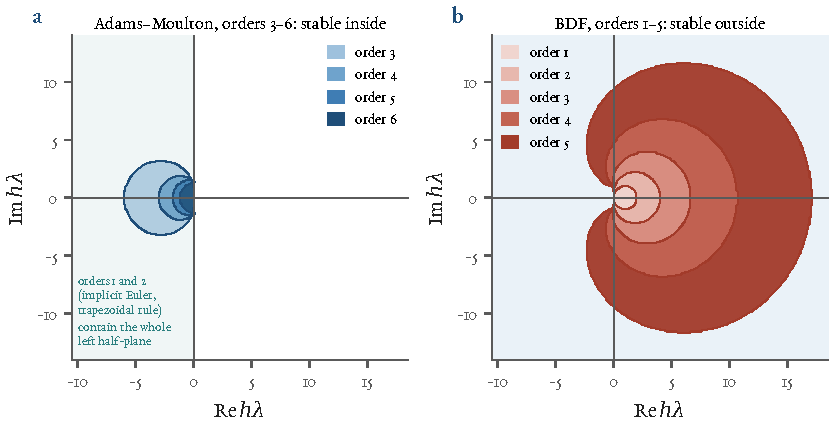
\includegraphics[width=\linewidth]{figures/ch02_stability.pdf}
\caption[Regions of absolute stability of the Adams and BDF formulas]{Regions of absolute stability, computed by a root test on a grid of $z=h\lambda$ for the fixed-step formulas to which CVODE's two families reduce when step and order are frozen.
(a) Adams--Moulton, orders 3--6: stable inside the lobes; orders 1 and 2 (implicit Euler, trapezoidal rule) are stable on the whole shaded left half-plane.
(b) BDF, orders 1--5: the filled lobes are the \emph{unstable} regions, everything else is stable. The coefficients were checked against their order conditions (exactness on polynomials), and
the computed half-angles $90^\circ,90^\circ,86.0^\circ,73.4^\circ,51.8^\circ$ of the stable wedge of BDF orders 1--5 agree with an independent boundary-locus computation ($86.03^\circ$, $73.35^\circ$, $51.84^\circ$), and the real-axis ends of panel~(a) were refined by bisection. CVODE changes step and order at run time: this figure is a guide to the families, not a law
for a run. Script \texttt{figures/ch02\_stability.py}.}\label{ch02:fig-stab}
\end{figure}

\Cref{ch02:fig-workprec} reports what the Python module does on three problems with closed-form solutions. Panel~(a) is ten periods of the harmonic oscillator, $19$ tolerances from $10^{-3}$ to $10^{-12}$ for each method. BDF gives a
clean line: the error falls smoothly as the tolerance is tightened. Adams is cheaper, by a factor of about seven where it matters (the cheapest Adams run with a final error below $10^{-8}$ used
$1\,880$ evaluations, the cheapest BDF run $12\,769$), and erratic: the run with $\mathrm{rtol}=10^{-5}$ used $704$ evaluations and ended with an error of $4.1\times10^{-5}$, the run with $10^{-6}$ used $3\,327$ and ended with
$5.0\times10^{-4}$, twelve times worse at $4.7$ times the cost. Local error control does not promise a monotone global error, and it does not deliver one.

\begin{figure}[tp]\centering
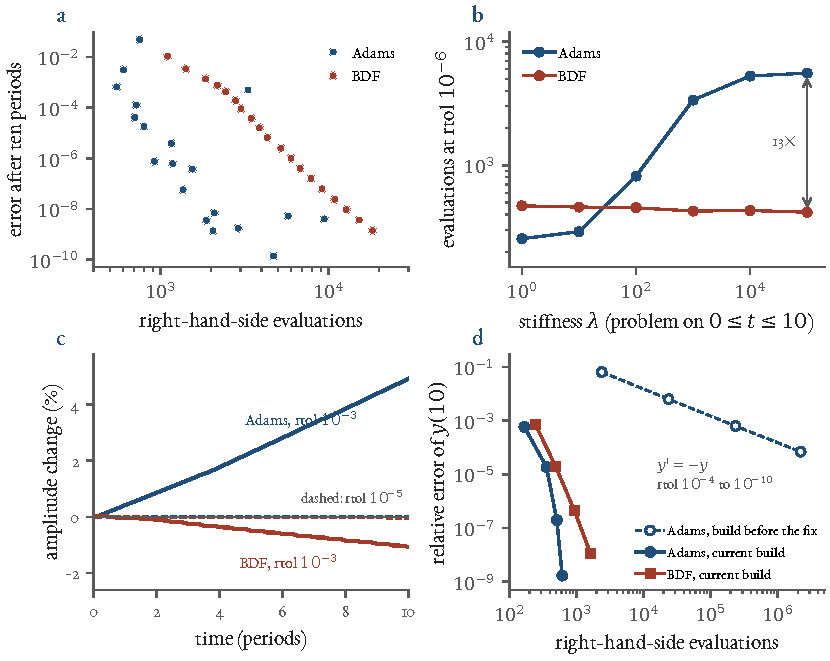
\includegraphics[width=\linewidth]{figures/ch02_workprecision.pdf}
\caption[CVODE on problems with closed-form solutions]{CVODE through the Python module on problems with closed forms; cost is the number of calls of the user's right-hand side, including the finite-difference Jacobian.
(a) Ten periods of $x''=-x$: error against cost, $19$ tolerances each.
(b) Prothero--Robinson problem $y'=-\lambda(y-\cos t)-\sin t$ \cite{ProtheroRobinson1974} on $0\le t\le10$ at $\mathrm{rtol}=10^{-6}$: cost against stiffness $\lambda$.
(c) Amplitude $|(x,v)|$ of the oscillator, exactly $1$, in independent runs to each time: at $\mathrm{rtol}=10^{-3}$ (full lines) and $10^{-5}$ (dashed).
(d) $y'=-y$: the module built on 26 September (before the Adams repair) and the current build.
Script \texttt{figures/ch02\_workprecision.py}; data \texttt{figures/ch02\_numbers.json}, key \texttt{B\_cvode}.}\label{ch02:fig-workprec}
\end{figure}

Panel~(b) is the stiffness test. The Prothero--Robinson problem has the smooth solution $y=\cos t$ for every $\lambda$, and a stiffness that grows with $\lambda$. At $\lambda=1$ Adams is cheaper than BDF ($255$ evaluations against $470$); at $\lambda=10^5$ it is
thirteen times dearer ($5\,565$ against $418$), and BDF's cost has not moved. A fixed-step stability bound would make the Adams cost grow in proportion to $\lambda$; it saturates instead. We did not trace why (a plausible reason is that the order selection falls back
to the A-stable orders 1 and 2, but the Python module does not report the order). What the measurement shows is the textbook division of labour with its cost attached: the non-stiff method is the cheaper one on the non-stiff problem, and an order of
magnitude dearer on the stiff one.

Panel~(c) matters for a Hamiltonian equation like \cref{ch02:eq-pgpe}: the oscillator has a conserved amplitude, as the PGPE has a conserved norm. After ten periods at $\mathrm{rtol}=10^{-3}$ the BDF solution has lost $1.1\,\%$ of its amplitude ($0.043\,\%$ at $10^{-5}$), as a dissipative method does on an oscillation (the stability theory is in
\cite{HairerWanner1996}), and in all $19$ runs of panel~(a) it ended with an amplitude below $1$. Adams errs in either direction depending on the tolerance (negative in $11$ of the $19$ runs); at $\mathrm{rtol}=10^{-3}$ it gained $4.9\,\%$, at $10^{-5}$ $0.004\,\%$. The integrator
has a bias of its own, which competes with the physics being simulated.

Panel~(d) is the defect of the previous section made visible. With the old module the error of Adams on the simplest problem of all, $y'=-y$, falls by a factor $10^{0.5}$ per decade of tolerance while the cost rises by the same
factor, the signature of a first-order method: at $\mathrm{rtol}=10^{-10}$ it needs $2.2\times10^{6}$ evaluations for an error of $6.9\times10^{-5}$, where the current build needs $616$ for $1.7\times10^{-9}$.
Every Adams run made with a build that predates the repair was a run of implicit Euler.

\section{The plane wave: a theorem and three integrators}\label{ch02:planewave}

The known answer is the one proved in \cref{ch02:theorem}. We take a plane wave on a periodic box of side $L=16$, $g=1$, density $1$, wave number $k=2\pi\cdot3/L=1.178$, so that
$\Omega=k^2/2+g=1.694$ (the one-mode form of the theorem is $\dot a=-\ii(k^2/2+g|a|^2)a$ with $|a|=1$), and integrate to $t=10$. The box below shows the call in the Rust engine.

\begin{rustbox}{qf-pgpe against the exact solution}
% CODE snippet2
\begin{lstlisting}[style=py]
import numpy as np, qf_pgpe

N, L, g, m = 32, 16.0, 1.0, 3
engine = qf_pgpe.Pgpe(N, L, g, 0.01)       # grid, box, coupling, time step
x = np.arange(N) * L / N
X, Y = np.meshgrid(x, x, indexing="ij")
k = 2 * np.pi * m / L
psi0 = np.exp(1j * k * X)                  # one mode, density 1
c = engine.run(np.ascontiguousarray(engine.modes(psi0)), 10.0)
omega = 0.5 * k ** 2 + g                   # omega = k^2/2 + g |a0|^2
exact = psi0 * np.exp(-1j * omega * 10.0)
err = np.abs(engine.psi(c) - exact).max()
print(f"plane wave, t = 10: max |psi - exact| = {err:.2e}")
\end{lstlisting}
% OUTPUT snippet2
\begin{lstlisting}[style=plainmono]
plane wave, t = 10: max |psi - exact| = 1.12e-08
\end{lstlisting}
\end{rustbox}

The error is $1.1\times10^{-8}$ at $\Delta t=0.01$. Panel~(a) of \cref{ch02:fig-plane} shows how it arises. For $\Delta t=0.02$, $0.01$, $0.005$ the error at $t=10$ is $1.8\times10^{-7}$, $1.1\times10^{-8}$ and $7.0\times10^{-10}$, in the numpy engine and in the
Rust engine alike (the two final states differ by $4\times10^{-14}$ at most, relative to the amplitude of the occupied mode); the ratios are $15.9$ and $16.0$. The error grows in proportion to $t$ and is a phase error: over the same run the norm of the state, hence the amplitude of the mode, changes by only $7\times10^{-12}$ (relative) at $\Delta t=0.01$; its dependence
on the step is that of a fourth-order scheme. At the programme's registered configuration (known answer K4: $N=64$, $L=32$, $\Delta t=0.005$, $t=10$, acceptance $10^{-9}$) both engines give $7.0\times10^{-10}$, the value of the stored first run. With $g=0$ the error
is $1.1\times10^{-14}$, rounding level.

\begin{figure}[tp]\centering
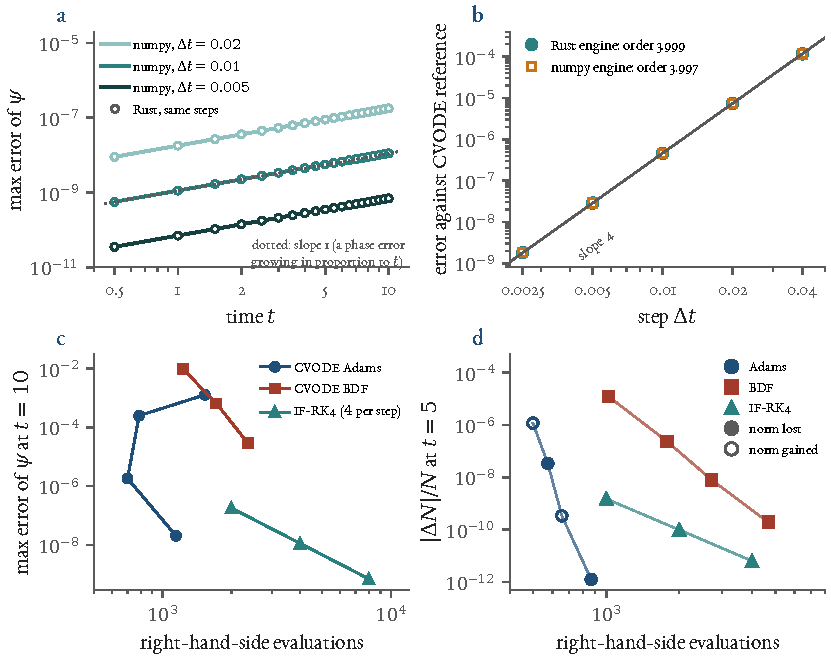
\includegraphics[width=\linewidth]{figures/ch02_planewave.pdf}
\caption[The exact plane wave against three integrators]{The exact plane wave against three integrators. (a) Error of the numpy IF-RK4 engine (lines) and of the Rust engine (circles) against $\psi_0\ee^{-\ii\Omega t}$, $N=32$, three steps; the error grows $\propto t$.
(b) Order of the IF-RK4 step measured against a CVODE (Adams, $\mathrm{rtol}=10^{-12}$) solution of the same right-hand side on a $16\times16$ grid, $t=1$: the registered Rust example (re-run; its output is identical to the stored file)
gives order $3.999$, the same test through the Python module and the numpy engine $3.997$; the errors of the two routes agree to $0.8\,\%$. (c) Cost against accuracy on the $16\times16$ plane wave. (d) Drift of the norm for a state with interacting modes
(a smooth three-mode superposition, $t=5$); filled symbols: norm lost, open: norm gained. Script \texttt{figures/ch02\_planewave.py}; keys \texttt{A\_order}, \texttt{C\_planewave}, \texttt{D\_invariants}.}\label{ch02:fig-plane}
\end{figure}

\paragraph{The order of the scheme, by an independent integrator.} The programme's registered control K2 asks that the energy drift of the scheme fall as $\Delta t^4$. The Rust port tests the order more directly, against a solution of the \emph{same} right-hand side by CVODE,
which shares with the engine nothing but that function. On a $16\times16$ grid ($49$ modes) with a smooth initial state, CVODE (Adams, $\mathrm{rtol}=10^{-12}$, $\mathrm{atol}=10^{-14}$) needs $482$ evaluations in $95$ steps, and the engine's error at $\Delta t=0.04,\dots,0.0025$ falls from $1.2\times10^{-4}$ to $1.8\times10^{-9}$ with successive
ratios $15.99$, $16.00$, $16.00$ and $15.97$ (a fourth-order scheme gives $16$). The fitted order is $3.999$. The reference run needs the Adams repair: with the old path it does not finish.

\paragraph{CVODE on the same wave.} Panel~(c) puts the integrators on one axis, for the $16\times16$ plane wave. CVODE's error is not monotone in its tolerance: Adams with $\mathrm{rtol}=10^{-4}$ spent $1\,530$ evaluations and ended with an error of $1.3\times10^{-3}$, with $10^{-6}$ it spent $788$ and ended with
$2.5\times10^{-4}$, with $10^{-8}$ $701$ and $1.8\times10^{-6}$, with $10^{-10}$ $1\,143$ and $2.0\times10^{-8}$; BDF at $10^{-8}$ spent $2\,364$ for $2.9\times10^{-5}$. At comparable error the engine's scheme needs about three times the
evaluations of CVODE-Adams at its tightest tolerance ($\approx3\,400$ for $2\times10^{-8}$, by interpolation) and, unlike CVODE, its error is monotone in the step. An evaluation of the engine's nonlinear term and one of CVODE's full right-hand side are not the same amount of work, and which integrator is cheaper is not the
point. The point is that all three reproduce the exact solution of the theorem to the precision each promises, which is what ``the program computes the function'' means in this case.

\paragraph{What does not conserve what.} Lean proves that the vector field has zero norm rate. Panel~(d) shows what integrators do with a conserved quantity. On a smooth state with interacting modes (the order-test state, evolved to $t=5$) the relative change of the norm under IF-RK4 at $\Delta t=0.02$, $0.01$, $0.005$ is
$-1.5\times10^{-9}$, $-9.8\times10^{-11}$ and $-6.3\times10^{-12}$: it falls by a factor $15$--$16$ per halving, so it is truncation error, not conservation. For CVODE-Adams at $\mathrm{rtol}=10^{-4}$ to $10^{-10}$ it is $+1.2\times10^{-6}$, $-3.4\times10^{-8}$,
$+3.3\times10^{-10}$ and $-1.2\times10^{-12}$, of either sign. For BDF it is $-1.2\times10^{-5}$, $-2.3\times10^{-7}$, $-7.9\times10^{-9}$ and $-1.9\times10^{-10}$, always a loss. No integrator conserves the norm; each
loses or gains it at a rate set by its own tolerance. The theorem is about the equation, and is true; the invariant is conserved by the program to a stated precision and no further.

\section{Where a theorem and a program part: aliasing}\label{ch02:alias}

The engine does not evaluate $N_k$ of \cref{ch02:eq-modes}. It evaluates $P[\,\mathrm{FFT}(|\psi|^2\psi)\,]$ on an $N\times N$ grid: transform to the grid, cube pointwise, transform back, keep the modes inside the projector. On the grid a
wave vector is a class modulo $N$, so a triple with $k_1-k_2+k_3=k+Nm$ for an integer vector $m\ne0$ is added to the same output mode as the triples with $m=0$. The engine's cubic term is a sum over all triples whose sum is congruent to $k$; the
Lean $N_k$ is a sum over the triples whose sum \emph{is} $k$. They are the same function exactly when no triple wraps.

The box below is the check: a literal transcription of the Lean definition for $G=\mathbb Z^2$, no wrap-around, and a comparison with the numpy engine's cubic term, rescaled to the units of the Lean statement ($a=c/N^2$ for the unnormalized FFT
convention of the engine). The transcription was written for this chapter and is not checked by Lean; its consistency is tested below.

\begin{rustbox}{The Lean definition of the cubic term, transcribed, against the engine}
% CODE lean_nl
\begin{lstlisting}[style=py]
def lean_nl(Lam, A):
    """Literal transcription of QuantumFluids.GPGalerkin.nl on Z^2:
         nl psi k = sum over k1, k2, k3 in Lam with k1 + k3 = k + k2 of
                    psi k1 * conj(psi k2) * psi k3        (no wrap-around)
       Lam: (m, 2) integer array of modes, A: (m,) amplitudes psi.
       Returns (table, B) with table[kx + B, ky + B] = nl psi (kx, ky)."""
    m = len(Lam)
    B = 3 * int(np.abs(Lam).max()) + 1               # sums reach 3 R
    size = 2 * B + 1
    re = np.zeros(size * size)
    im = np.zeros(size * size)
    for i in range(m):                               # k1 = Lam[i]
        k = Lam[i] - Lam[:, None, :] + Lam[None, :, :]       # k1 - k2 + k3
        idx = ((k[..., 0] + B) * size + (k[..., 1] + B)).ravel()
        v = (A[i] * np.conj(A)[:, None] * A[None, :]).ravel()
        re += np.bincount(idx, weights=v.real, minlength=size * size)
        im += np.bincount(idx, weights=v.imag, minlength=size * size)
    return (re + 1j * im).reshape(size, size), B
\end{lstlisting}
and, in the driver, the engine's term in the same units:
% CODE engine_vs_lean
\begin{lstlisting}[style=py]
a = np.zeros((N, N), dtype=complex)
a[s.P] = A                  # psi_k, the units of the Lean statement
c = a * N ** 2              # the engine's unnormalized FFT amplitudes
# the engine's cubic term, in the units of nl:
nl_eng = s.nonlin(c) / (-1j * g * N ** 2)
\end{lstlisting}
% OUTPUT snippet3
\begin{lstlisting}[style=plainmono]
cutoff 0.500  modes 197  max|engine-nl|/max|nl| = 7.85e-16  differing: 0
cutoff 0.500  modes 197  max|engine-nl|/max|nl| = 1.15e-03  differing: 4
cutoff 0.667  modes 357  max|engine-nl|/max|nl| = 1.53e-01  differing: 348
\end{lstlisting}
The three lines are the cases of \cref{ch02:fig-bridge,ch02:fig-rates}: $N=32$, $L=16$, a random complex state on the retained modes (seed fixed); the first with the four extreme modes empty, the second with all modes filled, the third at the larger cutoff.
Function \texttt{lean\_nl} and driver \texttt{bridge\_case} of \texttt{figures/ch02\_compute.py}, run by \texttt{figures/ch02\_snippets.py}.
\end{rustbox}

With the cutoff at one half of the largest wave number, the engine's cubic term equals the Lean definition to $7.9\times10^{-16}$, rounding, on a state whose four extreme modes are empty. With those modes filled, four modes of the $197$ differ, by
$1.1\times10^{-3}$ at most (relative to the largest value of $N_k$). At two thirds, $348$ of $357$ modes differ, by up to $15\,\%$ of the largest value. The geometry of \cref{ch02:fig-bridge}(a,b) explains all three. A triple reaches $|k_1-k_2+k_3|\le3R$ if the retained modes lie in a disc of radius $R$
(in index units); the periodic images of that reach-disc, displaced by $N$ along the axes, intrude into the retained disc when $3R+R>N$. So the engine's function equals $N_k$ for \emph{every} state when $4R<N$, that is, $k_{\rm cut}<k_{\max}/2$. At $4R=N$, which is the engine's
default cutoff, the discs touch at four points: the four modes $\pm(N/4,0)$, $\pm(0,N/4)$, each fed by a single wrapped triple, for the mode $(-N/4,0)$ the triple $k_1=k_3=-k_2=(N/4,0)$, as the data show. For a quadratic nonlinearity the reach is $2R$, the condition is $3R\le N$, and
one recovers the two-thirds rule \cite{Orszag1971}; for the cubic term of the PGPE that rule is wrong, as the programme found.

\begin{figure}[tp]\centering
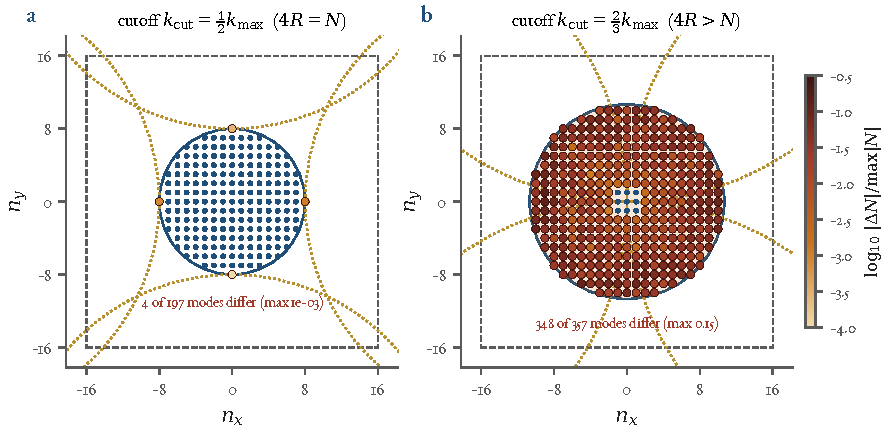
\includegraphics[width=\linewidth]{figures/ch02_bridge.pdf}
\caption[The same equation in the two languages]{The same equation in the two languages: where the engine's cubic term and the literal Lean definition coincide. Retained modes in the index plane ($N=32$), coloured by the difference between the two on a random state with all modes filled; blue: equal to rounding.
Dashed square: the Nyquist box; dotted arcs: the periodic images of the disc of radius $3R$ reached by the triple sums; orange shading: the modes the images cover. The cutoffs are $\frac12k_{\max}$ (a) and $\frac23k_{\max}$ (b).
Script \texttt{figures/ch02\_bridge.py}; key \texttt{E\_bridge}.}\label{ch02:fig-bridge}
\end{figure}



Panel~(a) of \cref{ch02:fig-rates} puts the theorems against the engine. For the literal definition both rates vanish to rounding (below $10^{-17}$ relative to the sum of the moduli of the terms) in all three cases, as \Lthm{GPGalerkin}{mass_rate_zero} and \lean{momentum\_rate\_zero} say they must.
That the transcription is the Lean object is tested by the identity of \Lthm{GPGalerkin}{pairing_eq_sum}, which the transcription satisfies: $Q=1.403114631989707$ against $\sum_q|A_q|^2=1.4031146319897068$, with imaginary part $2.8\times10^{-17}$.
For the engine, the mass rate is zero to rounding even where triples wrap: by Parseval on the grid
\[
\sum_k\overline{a_k}\,P\bigl[\mathrm{FFT}(|\psi|^2\psi)\bigr]_k=\sum_x|\psi(x)|^4 ,
\]
a real number, wrapped or not (an argument, not a Lean theorem). The momentum rate is not zero: $1.6\times10^{-17}$ with the extreme modes empty, $2.3\times10^{-5}$ with them filled, $4.1\times10^{-3}$ at the larger cutoff.
The theorem and the program agree exactly where the theorem's hypothesis holds, and part company where it does not: there the grid is $\mathbb Z_N^2$, and \lean{no\_momentum\_on\_torus} says that no additive momentum exists on it.

\begin{figure}[tp]\centering
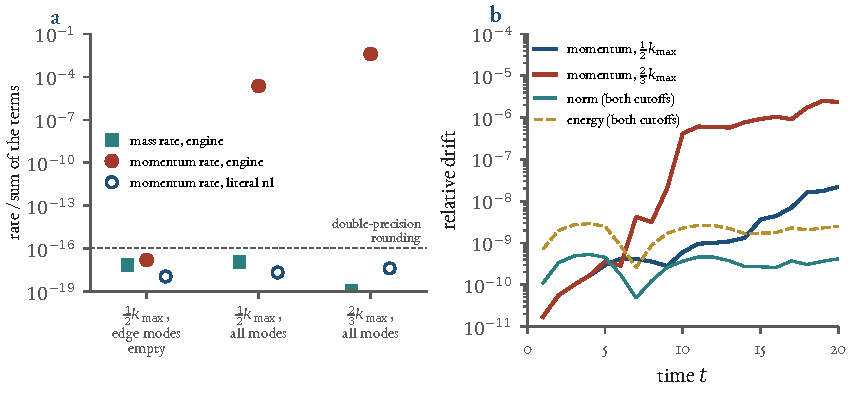
\includegraphics[width=\linewidth]{figures/ch02_rates.pdf}
\caption[Theorems and engine, in rates and in time]{Theorems and engine, in rates and in time. (a) Instantaneous rates for the engine and for the literal definition, in the three cases of the text: of the mass, $|\sum_k\mathrm{Im}(\overline{\psi_k}G_k)|\big/\sum_k|\overline{\psi_k}G_k|$, and of the momentum, the same with the weight $p(k)=k_x$ in numerator and
denominator; the Lean theorems say that the literal definition gives zero. The point on the lower edge is exactly $0$. (b) Drift of the invariants along an IF-RK4 run ($\Delta t=0.01$) from one smooth random state at $N=32$, for the two cutoffs; norm and energy are the same for both.
Script \texttt{figures/ch02\_bridge.py}; key \texttt{E\_bridge}.}\label{ch02:fig-rates}
\end{figure}

Integrated in time (panel~(b) of \cref{ch02:fig-rates}), one smooth random state ($N=32$, $L=16$, energy $0.6$ per particle, seed $3$) evolved by IF-RK4 at $\Delta t=0.01$ with the two cutoffs has at $t=10$ a relative norm drift of $3.7\times10^{-10}$ and an energy drift of $2.3\times10^{-9}$, the same at both cutoffs,
and a momentum drift (relative to $\sum_k|k||c_k|^2$) of $6.0\times10^{-10}$ at $\frac12k_{\max}$ and $4.2\times10^{-7}$ at $\frac23k_{\max}$; at $t=20$ the momentum drifts are $2.2\times10^{-8}$ and $2.4\times10^{-6}$, norm and energy $4.2\times10^{-10}$ and $2.5\times10^{-9}$ for both. Norm and energy do not see the aliasing;
momentum does, separating the two cutoffs by two to three orders of magnitude. This is a modest reproduction of the programme's control, on a smooth state and a $32^2$ grid where the recorded failure ($8.5$, one per cent) was a random high-energy state on $64^2$. The drift at the one-half cutoff is not zero either; we did not separate the
truncation error of the scheme from the effect of the four edge modes, which the evolving state may populate.

\section{What each instrument can see}\label{ch02:see}

\Cref{ch02:tab-see} sorts the statements of this chapter by the instrument that can establish them. The rows for the norm and the plane wave are the reason the programme runs controls of several kinds: a proof of the right theorem cannot detect that the program evaluates another function, and the control that
can, the momentum, is one that the norm and the plane wave are blind to.

\begin{table}[t]\centering\footnotesize
\begin{tabular}{p{0.14\linewidth}p{0.24\linewidth}p{0.30\linewidth}p{0.19\linewidth}}\toprule
property & Lean (a statement for every $\Lambda$ and state) & registered control and independent integrators & what it caught here\\\midrule
norm rate $=0$ & \lean{mass\_rate\_\allowbreak zero} (library), any $\Lambda$ & K1: drift $4.2\times10^{-10}$; engine rate at most $1.1\times10^{-17}$ in all cases & nothing: blind to aliasing\\
exact plane wave & \lean{planeState\_\allowbreak solves\_\allowbreak galerkin} (new) & K4: $7.0\times10^{-10}$; numpy, Rust and CVODE agree & nothing: blind to aliasing\\
momentum rate $=0$ & \lean{momentum\_\allowbreak rate\_\allowbreak zero} (new), needs an additive $p$ & K3: drift $8.5$ in the first run; rate $4.1\times10^{-3}$ at $\frac23k_{\max}$ & the wrong cutoff rule\\
order of IF-RK4 & none in the library & K2 (energy drift $\propto\Delta t^4$); error against CVODE: order $3.999$ & the Adams defect: the reference run cannot finish without the repair\\
the program computes the function & none: a statement about a program & transcription of \lean{nl} against the engine & $4$ modes differ at $\frac12k_{\max}$, $348$ at $\frac23k_{\max}$\\\bottomrule
\end{tabular}
\caption{Which instrument can establish what. The first two controls pass with or without aliasing; the third separates the cutoffs.}\label{ch02:tab-see}
\end{table}

\begin{honestbox}
\begin{itemize}
\item \textbf{Proved} (Lean, kernel-checked, standard axioms only). For every finite mode set in every additive group: the mass-rate identity and the non-negativity of the quartic interaction (library, \lean{GPGalerkin}); the exact plane wave solves the
Galerkin system; the momentum-rate identity for every additive weight; no non-zero additive map exists on $\mathbb Z_N\times\mathbb Z_N$ (new, \texttt{book/lean/Ch02\_Galerkin.lean}). These are statements about the mathematical function $N_k$ and about rates at an instant: not about existence of solutions,
not about conservation along a solution, not about any program.
\item \textbf{Measured or simulated.} The engine's cubic term equals a transcription of $N_k$ to $8\times10^{-16}$ when no triple wraps (one random state per case, $N=32$); three integrators reproduce the exact plane wave to the precisions stated; the order of the IF-RK4 step is $4.00$ (fitted $3.999$ and $3.997$);
CVODE's costs and errors on the stated problems, with the build described above.
\item \textbf{Not established.} That the transcription equals the Lean object is a correspondence made by hand and tested by one identity, not proved; nothing proves the Rust code; agreement of rusty-SUNDIALS with the C library is not claimed; the stability regions are fixed-step guides; the Adams cost on the stiff problem is
measured but its cause is not traced; the momentum drift at the one-half cutoff mixes truncation error and edge-mode aliasing, which we did not separate.
\item \textbf{An analogy, not a result.} The division into ``Lean sees'' and ``the solver sees'' is a classification of this chapter's cases, not a theorem about methods.
\item \textbf{What failed.} The pre-registered rule $k_{\rm cut}=\frac23k_{\max}$ was wrong for a cubic term, and the momentum control caught it. The pre-registration's sentence that the three conservation laws were library theorems was wrong for one of them and incomplete for the other two.
The Adams path of rusty-SUNDIALS was implicit Euler until it was repaired, and the module in the programme's virtual environment still is. The first draft of this chapter's Lean file contained a proof that did not compile, and its audit line carried \lean{sorryAx}.
\end{itemize}
\end{honestbox}

\paragraph{Exercise 1.} In a commutative ring with $e^3=0$ show that $(1+e)(1-e+e^2)=1$ by \lean{linear\_combination}, then change the sign of the $e^2$ term and read the reply. \emph{Hint.} The goal minus the coefficient times the hypothesis must be an identity of rings: $(1+e)(1-e+e^2)-1=e^3$, so the coefficient is $1$.

\paragraph{Exercise 2.} In the first box of \cref{ch02:solver} replace the oscillator by the Prothero--Robinson problem with $\lambda=10^4$: right-hand side \lean{[-lam * (y[0] - math.cos(t)) - math.sin(t)]}, initial value \lean{[1.0]}, end time $10$, tolerances \lean{1e-6} and \lean{1e-8}.
Count the calls for both methods and compare with \cref{ch02:fig-workprec}(b); then set \lean{max\_steps} to $300$ and read the reply. \emph{Hint.} With the build used here the counts are $5\,270$ (Adams) and $431$ (BDF). With \lean{max\_steps = 300} BDF still finishes, and Adams stops with
\lean{maximum steps exceeded (300) at t=1.77}: \lean{max\_steps} counts internal steps, and Adams needs more than $300$ of them for the first $1.8$ time units.

\paragraph{Exercise 3.} (a) On a grid with $N=16$ the retained set at $k_{\rm cut}=\frac12k_{\max}$ contains $(\pm4,0)$ and $(0,\pm4)$. Find the single wrapped triple that feeds the mode $(-4,0)$, and use the geometry of \cref{ch02:fig-bridge} to say for which cutoffs the cubic term of the engine equals $N_k$ for \emph{every} state
when $N=16$ (answer in index units). (b) Show that the engine's mass rate $\sum_k\mathrm{Im}(\overline{a_k}G_k)$ vanishes for every state, wrapped or not, and explain why the same argument cannot give momentum.
\emph{Hint.} (a) Look for $k_1+k_3-k_2=(-4,0)+(16,0)$ with all three modes of norm $4$; the condition is $4R<N$. (b) Parseval on the grid turns $\sum_k\overline{a_k}P[\mathrm{FFT}(|\psi|^2\psi)]_k$ into $\sum_x|\psi(x)|^4$; for momentum you need a function of $k$ that is additive modulo $N$, and \lean{no\_momentum\_on\_torus} says there is none.

\section{Notes and further reading}\label{ch02:notes}

For Lean, \emph{Theorem Proving in Lean~4} \cite{TPIL4} introduces the language and \emph{Mathematics in Lean} \cite{MIL} the use of Mathlib; the kernel and the elaborator are described in \cite{deMoura2021}. For the numerics, Hairer, N{\o}rsett and Wanner \cite{HairerNorsettWanner1993} treat Adams methods and
Hairer and Wanner \cite{HairerWanner1996} stiffness, BDF and absolute stability, with Dahlquist's paper on A-stability \cite{Dahlquist1963} as the source of the notion; Prothero and Robinson \cite{ProtheroRobinson1974} define the stiff test problem used here; the SUNDIALS suite is described in \cite{Hindmarsh2005}. The
pseudo-spectral treatment of the projected equation and the aliasing rules are in \cite{Blakie2008} and \cite{Orszag1971}. The solver is described, with its cross-checks and its performance, in the software paper \cite{Callens2026sw}, the Lean library in \cite{Callens2026lib}. Everything in this chapter can be regenerated: the numbers by
\texttt{figures/ch02\_compute.py} (parts A to E, into \texttt{figures/ch02\_numbers.json}), the code boxes by \texttt{figures/ch02\_snippets.py}, the figures by the four \texttt{figures/ch02\_*.py} scripts, the Lean files with
\texttt{lake env lean} on the three files \texttt{book/lean/Ch02\_*.lean}; the Python module of the current build is made by \texttt{book/rust/ch02\_build\_py.sh} (the copy used here, with its checksum, is in \texttt{/mnt/data/xdev-cache/rs\_py\_5db8041}). The next chapters use the two languages without
re-introducing them; \cref{ch10} returns to the question of how far each instrument can be trusted.
}
\part{Bose Superfluids}
\IfCh{ch11}{\input{chapters/ch11}}
\IfCh{ch03}{\chapter{From the Wave Function to the Fluid: Circulation and Vortices}\label{ch03}
% ---- local macros (unique names: chapters are combined into one document) -------------------------------------------
\InputIfFileExists{figures/ch03_numbers.tex}{}{\PackageWarning{ch03}{figures/ch03_numbers.tex is missing}}
\newcommand{\cthreeNum}[1]{\ifcsname cthree@#1\endcsname\csname cthree@#1\endcsname\else\textbf{??#1??}\PackageWarning{ch03}{number #1 is undefined}\fi}
\newcommand{\cthreeCode}[1]{\path{#1}}
\newlength{\cthreeOldES}\setlength{\cthreeOldES}{\emergencystretch}\setlength{\emergencystretch}{2.5em}
\let\cthreeOldTopFrac\topfraction\let\cthreeOldTextFrac\textfraction\let\cthreeOldFloatFrac\floatpagefraction
\renewcommand{\topfraction}{0.9}\renewcommand{\textfraction}{0.1}\renewcommand{\floatpagefraction}{0.85}% large figures stay on text pages instead of forming float pages

\section{An observation: circulation comes in whole units}\label{ch03:obs}

In 1961 W.~F.~Vinen detected single quanta of circulation in superfluid $^4$He with a vibrating wire; the quantum had the size that had been anticipated, $h/m$, with $m$ the mass of a helium atom \cite{Vinen1961,Zieve2023}.
Eighteen years later Yarmchuk, Gordon and Packard recorded photographically the positions of the quantized vortex lines in rotating superfluid helium and observed stationary arrays \cite{Yarmchuk1979}.
What these experiments measure is a number that no classical fluid has. The circulation $\Gamma=\oint\mathbf u\cdot\dd\mathbf l$ of the velocity around a closed curve drawn in the liquid takes only the values $0,\pm\kappa,\pm2\kappa,\dots$, where
\begin{equation}\label{ch03:eq-kappa}
  \kappa=\frac{h}{m}.
\end{equation}
The number is remarkable for what it does not contain. It is built from Planck's constant and the mass of one atom; no interaction strength, no density, no temperature enters. For $^4$He, with the exact SI value of $h$ and the atomic mass $m=\cthreeNum{mHeU}$~u (NIST), it is $\kappa=\cthreeNum{kappaHeFour}\times10^{-8}\ \mathrm{m^2/s}$ (computed in \texttt{figures/ch03\_compute.py}). In a vessel rotating at angular velocity $\Omega$ the quantized lines must on average imitate solid-body rotation, whose circulation per unit area is $2\Omega$; Feynman's counting \cite{Feynman1955} then gives an areal density $2\Omega/\kappa$ of lines, which is $\cthreeNum{feynmanDens}$ per cm$^2$ at $\Omega=1$~rad/s.

How can a complex wave function know about circulation? A wave function has a phase, and the velocity of the fluid it describes is the gradient of that phase. A gradient has no circulation, unless the phase cannot be defined everywhere, and a single-valued wave function can fail to define a phase only where it vanishes. A vortex is such a point. That is the chapter in three sentences; the pages that follow make each precise in the way of this book, as a statement a proof assistant has checked, as a computation the solver has run and, where an experiment exists, as a number to compare with it.

\begin{keybox}[What the chapter establishes]
\begin{enumerate}
\item \textbf{Circulation is quantized:} around a closed loop it is $w\kappa$ with $w$ an integer; sampled, this is a theorem about sums of principal phase differences (Lean, \cref{ch03:circ}).
\item \textbf{A vortex is a zero of $\psi$ with a winding number}, which the detector of every simulation code finds once the sampling resolves the phase (Lean, \cref{ch03:circ}); the solver shows how fine that is (\cref{ch03:counting}).
\item \textbf{Vortices are carried by the flow of the others:} a pair of separation $d$ moves at $\hbar/(md)$ in the plane; in a periodic box the integers that wind the phase around the torus add a uniform flow, $\cthreeNum{ubarOverV}\%$ of that speed at $d\approx12\xi$. The solver reproduces the corrected speed to about a percent for $d\ge6\xi$ and follows two leapfrogging pairs against a point-vortex model integrated with CVODE (\cref{ch03:speed,ch03:leap}).
\end{enumerate}
\end{keybox}

\begin{godfrinbox}{the other kind of excitation}
The experiments of Henri Godfrin and his collaborators probe quantum fluids through their excitations: inelastic neutron scattering at the Institut Laue--Langevin measured the dispersion relation of the phonon--maxon--roton excitations of superfluid $^4$He (Phys.\ Rev.\ B \textbf{103}, 104516 (2021), spectrometer IN5) \cite{Godfrin2021} and the density waves of two-dimensional liquid $^3$He (Nature \textbf{483}, 576 (2012)) \cite{Godfrin2012}.
In the linear theory such excitations are small oscillations about the uniform state, with a velocity that is the gradient of a single-valued phase: irrotational, without circulation. The vortices of this chapter are the other kind of excitation, states whose phase is \emph{not} single valued around a loop, which no small-amplitude wave can create or remove. Both live in the same $\psi$. \Cref{ch05} treats the first kind; the superfluid transition of a two-dimensional $^4$He film, measured by Bishop and Reppy \cite{BishopReppy1978} and described by the unbinding of vortex--antivortex pairs \cite{KosterlitzThouless1973}, is where the two meet (\cref{ch06}). Nothing here claims that those experiments observed vortices.
\end{godfrinbox}

\section{The wave function as a fluid}\label{ch03:madelung}

The model of the superfluid used throughout the book is the Gross--Pitaevskii equation \cite{Gross1961,Pitaevskii1961},
\begin{equation}\label{ch03:eq-gp}
  \ii\hbar\,\partial_t\psi=-\frac{\hbar^2}{2m}\nabla^2\psi+g\,|\psi|^2\psi,
\end{equation}
with $g>0$ the strength of a contact repulsion. For a dilute Bose gas at zero temperature it is the equation of the condensate; for liquid helium it is a model with the right structure (a complex order parameter, a compressible fluid, quantized circulation) and not the right numbers, since the core of a vortex in the liquid is of atomic size. The uniform state of density $n_0$ has two natural scales: the healing length $\xi=\hbar/\sqrt{mgn_0}$ and the speed of sound $c=\sqrt{gn_0/m}$. In the units $\hbar=m=g=n_0=1$ used by the solver both are $1$, so is the unit of time $\xi/c$, and the quantum of circulation is $\kappa=2\pi$.

Write the wave function in polar form, $\psi=\sqrt n\,\ee^{\ii S}$, with $n=|\psi|^2$ the density and $S$ the phase, and define the velocity
\begin{equation}\label{ch03:eq-u}
  \mathbf u=\frac{\hbar}{m}\nabla S .
\end{equation}
Substituting into \eqref{ch03:eq-gp} and separating the real and imaginary parts gives two real equations, found by Madelung in 1927 \cite{Madelung1927}:
\begin{align}
  \partial_t n+\nabla\!\cdot(n\,\mathbf u)&=0, \label{ch03:eq-cont}\\
  m\big(\partial_t\mathbf u+(\mathbf u\!\cdot\!\nabla)\mathbf u\big)&=-\nabla\big(g\,n+Q\big),\qquad Q=-\frac{\hbar^2}{2m}\,\frac{\nabla^2\sqrt n}{\sqrt n}. \label{ch03:eq-euler}
\end{align}
The first is conservation of mass. The second is Euler's equation for an inviscid compressible fluid of pressure $P=gn^2/2$, plus a \emph{quantum pressure} $Q$, which is all that remains of $\hbar$ once $\psi$ is written this way, and plus a constraint that no classical fluid obeys: $\mathbf u$ is a gradient, so $\nabla\times\mathbf u=0$ wherever $S$ is smooth. All the vorticity of a quantum fluid sits where $S$ is not smooth. The dictionary is short: density $n=|\psi|^2$, velocity $\mathbf u=(\hbar/m)\nabla S$, pressure $gn^2/2$, quantum pressure $Q$ (local, important only at scales $\lesssim\xi$), and vortex cores where $\psi=0$ and $S$ is undefined.

What the proof assistant says about it is limited and exact. The library does not contain \eqref{ch03:eq-cont} and \eqref{ch03:eq-euler}, which are textbook and derived above in two lines. What \texttt{MadelungSplit} proves is the algebra underneath: the squared gradient of $\psi=a\,\ee^{\ii S}$ splits into an amplitude part and a phase part, so the kinetic energy density of $\psi$ is the sum of the quantum-pressure term and the classical kinetic energy of the fluid.

\begin{leanbox}{MadelungSplit}
\begin{lstlisting}[style=lean,basicstyle=\ttfamily\footnotesize]
-- namespace QuantumFluids.Madelung
/-- **Kinetic-energy density split with physical constants.** With `rho = a^2` and superfluid
velocity components `u_i = (hbar/m) d_i S`, the kinetic energy density
`(hbar^2/2m) |grad psi|^2` equals the quantum-pressure term `(hbar^2/2m) |grad a|^2`
plus the hydrodynamic term `(m/2) rho |u|^2`. -/
theorem kinetic_density_split (ħ m a ga gS : ℝ) (hm : m ≠ 0) :
    ħ ^ 2 / (2 * m) * (ga ^ 2 + a ^ 2 * gS ^ 2)
      = ħ ^ 2 / (2 * m) * ga ^ 2 + m / 2 * a ^ 2 * (ħ / m * gS) ^ 2
\end{lstlisting}
\end{leanbox}

Here \texttt{ga} and \texttt{gS} stand for the components of $\nabla a$ and $\nabla S$ with $a=\sqrt n$. The statement of which this is the bookkeeping, \Lthm{MadelungSplit}{madelung_gradient_split}, is proved for an amplitude--phase wave function on $\mathbb R^n$ under the hypothesis that $a$ and $S$ are differentiable at the point; that hypothesis is genuine, and it is exactly what fails at a vortex core, where $a=0$ and $S$ is undefined. The module \texttt{MadelungNSE} restates the Madelung velocity in the vocabulary of a Lean formalisation of the Navier--Stokes problem statement and proves $\operatorname{div}\mathbf u=(\hbar/m)\Delta S$ there (\Lthm{MadelungNSE}{divergence_madelungVelocity}): bookkeeping, not a result about Navier--Stokes, which puts the two fluids in one formalism. That \eqref{ch03:eq-cont} and \eqref{ch03:eq-euler} look like the classical equations is an analogy; \cref{ch03:honest} says what the quantum fluid has that the classical one has not.

\section{Quantized circulation}\label{ch03:circ}

The circulation of the Madelung velocity \eqref{ch03:eq-u} around a closed curve $C$ on which $\psi\neq0$ is
\begin{equation}\label{ch03:eq-gamma}
  \Gamma(C)=\oint_C\mathbf u\cdot\dd\mathbf l=\frac{\hbar}{m}\oint_C\nabla S\cdot\dd\mathbf l=\frac{\hbar}{m}\,\Delta_C S ,
\end{equation}
that is, $\hbar/m$ times the change of the phase around $C$. The wave function must return to itself after one turn, so $S$ does so modulo $2\pi$: $\Delta_CS=2\pi w$ with $w$ an integer, and $\Gamma=w\,h/m=w\kappa$. This is the argument of Onsager \cite{Onsager1949} and Feynman \cite{Feynman1955}, and the integer $w$ is the \emph{winding number} of $\psi$ along $C$. It is topological: neither $g$ nor $n$ nor the dynamics enters, which is why the same quantum appears in a liquid and in a dilute gas.

Neither a simulation nor a photograph provides $S$ along a curve, only $\psi$ at points. The method of essentially every code that finds vortices, including this book's, is the following. Take points $\mathbf x_0,\dots,\mathbf x_n=\mathbf x_0$ along the loop, read the phases $\theta_i=\arg\psi(\mathbf x_i)$, replace each step $\theta_{i+1}-\theta_i$ by its principal value $\mathrm{pdiff}(\theta_i,\theta_{i+1})\in(-\pi,\pi]$, and add. Two questions arise. Is the sum a multiple of $2\pi$ whatever the sampling? And is the multiple the winding number of the continuous field? The library answers the first in \texttt{VortexWinding} and \texttt{QuantizedCirculation}, the second in \texttt{ContinuumWinding}.

\paragraph{Layer one: an identity of sums.} The principal difference differs from the true step by an integer multiple of $2\pi$ (\Lthm{VortexWinding}{pdiff_eq}), and on a closed loop the true steps telescope to $\theta_n-\theta_0=0$. Hence the sum of principal differences is an integer multiple of $2\pi$ (\Lthm{VortexWinding}{loop_sum_eq_mul}), and multiplying by $\hbar/m$ gives the following.

\begin{leanbox}{QuantizedCirculation}
\begin{lstlisting}[style=lean,basicstyle=\ttfamily\footnotesize]
-- namespace QuantumFluids.Circulation ; pdiff comes from QuantumFluids.VortexWinding
noncomputable def kappa (hbar m : ℝ) : ℝ := 2 * π * hbar / m

noncomputable def circulation (hbar m : ℝ) (S : ℕ → ℝ) (n : ℕ) : ℝ :=
  (hbar / m) * ∑ i ∈ Finset.range n, pdiff (S i) (S (i + 1))

/-- **Circulation is quantized.** Around any closed loop the circulation is an integer multiple of
the quantum `kappa`. -/
theorem circulation_quantized (hbar m : ℝ) (S : ℕ → ℝ) (n : ℕ) (hclosed : S n = S 0) :
    ∃ q : ℤ, circulation hbar m S n = (q : ℝ) * kappa hbar m := by
  obtain ⟨q, hq⟩ := loop_sum_eq_mul S n hclosed
  refine ⟨q, ?_⟩
  unfold circulation kappa
  rw [hq]
  ring
\end{lstlisting}
\end{leanbox}

The proof is the four lines shown; the content is in \Lthm{VortexWinding}{loop_sum_eq_mul}, whose proof is the telescoping argument just given (not shown). The same module proves \Lthm{QuantizedCirculation}{abs_circulation_ge}, that a nonzero circulation has magnitude at least $\kappa$ (no fraction of a quantum), and \Lthm{QuantizedCirculation}{circulation_quantum_attained}, that $\kappa$ itself is attained, by an explicit four-point loop whose last step wraps around by $2\pi$, the branch behaviour that \texttt{pdiff} exists to handle. The bound is therefore sharp. What neither theorem says is that the integer has anything to do with the field: for an arbitrary sequence of phases the sum is just as much a multiple of $2\pi$.

\paragraph{Layer two: the integer is the right one.} The next theorem closes that gap for a loop of field values.

\begin{leanbox}{ContinuumWinding}
\begin{lstlisting}[style=lean,basicstyle=\ttfamily\footnotesize]
-- namespace QuantumFluids.ContinuumWinding ; I = unit interval, [0,1]
/-- The `i`-th of `n` uniform sample points of the unit interval. -/
noncomputable def sample (n i : ℕ) : I := Set.projIcc 0 1 zero_le_one ((i : ℝ) / n)

/-- **The phase-winding vortex detector is correct.** For a continuous, nowhere-vanishing, closed loop
of field values, the sampled principal-branch loop sum of `arg` equals `2π` times the degree of the
loop, for every fine enough uniform sampling. -/
theorem detector_correct (c : C(I, ℂ)) (hne : ∀ t, c t ≠ 0) (hclosed : c 1 = c 0) :
    ∃ w : ℤ, ∃ n₀ : ℕ, 0 < n₀ ∧ ∀ n ≥ n₀,
      ∑ i ∈ Finset.range n, pdiff (Complex.arg (c (sample n i))) (Complex.arg (c (sample n (i + 1))))
        = (w : ℝ) * (2 * π)
\end{lstlisting}
\end{leanbox}

In words: if the loop $t\mapsto c(t)$ is continuous, closed and never zero, there are an integer $w$ (its degree) and a size $n_0$ such that every uniform sampling with $n\ge n_0$ points gives exactly $2\pi w$. The proof idea (abridged): the angle of $c$ is a closed loop on the circle $\mathbb R/2\pi\mathbb Z$; lift it to $\mathbb R$ along the covering map (Mathlib's path lifting); the lift is uniformly continuous on a compact interval (Heine--Cantor), so for large $n$ consecutive samples differ by less than $\pi$, every principal difference \emph{is} the true difference of the lift, the sum telescopes, and it equals the total change of the lift, $2\pi w$.

Two things the theorem does not give are what the solver supplies. It does not give $n_0$, which depends on how fast $c/|c|$ turns; the file says so. And its hypothesis \cthreeCode{hne} is where a vortex enters: on a loop through a zero of $\psi$ the lift, the degree and the theorem cease to exist. The failure mode of the standard algorithm is also a theorem: traversing an edge forth and back cancels exactly, except when the phase difference is exactly $\pi$, where both directions return $+\pi$ and add up to $2\pi$ (\Lthm{VortexWinding}{pdiff_add_rev_eq_two_pi_iff}); then two neighbouring plaquettes of a grid fail to cancel their shared edge and a spurious winding can appear. No true phase step between neighbouring samples may reach $\pi$.

\section{The vortex}\label{ch03:vortex}

\subsection{A vortex is a zero of \texorpdfstring{$\psi$}{psi}}\label{ch03:zero}Let a loop $C$ have winding $w\neq0$. If $\psi$ did not vanish anywhere on the disc bounded by $C$, shrinking $C$ continuously to a point would keep the winding an integer-valued continuous function, hence constant, and a point has winding zero. So $\psi$ vanishes somewhere inside. This is standard topology and it is \emph{not} in the library: the pinned Mathlib has no argument principle for general continuous maps, as the module \texttt{ContinuumWinding} says. What the library has is the discrete substitute of \cref{ch03:scale} below.

\subsection{Structure of one vortex}Around a singly quantized vortex at the origin the phase is the azimuth, $S=\theta$, so $\mathbf u=\hbar/(mr)\,\hat{\boldsymbol\theta}$ \emph{exactly}, whatever the density. The wave function is $\psi=\sqrt{n_0}\,f(r)\,\ee^{\ii\theta}$ where, in units of $\xi$,
\begin{equation}\label{ch03:eq-profile}
  f''+\frac{f'}{r}-\frac{f}{r^2}+2f(1-f^2)=0,\qquad f(0)=0,\quad f(\infty)=1 .
\end{equation}
A boundary-value solution (\texttt{figures/ch03\_gpvortex.py}) gives $f\simeq\cthreeNum{fSlope}\,r/\xi$ near the axis and $n=n_0f^2\simeq n_0\,(1-\xi^2/2r^2)$ far from it. The velocity decays like $1/r$ and the density disturbance like $1/r^2$: the flow of a vortex is long ranged, its core short ranged. By the split of the previous section the energy inside a disc of radius $R\gg\xi$ about the core then has a flow part $\int\frac12mn_0u^2\,\dd^2x=\pi(\hbar^2n_0/m)\ln(R/\xi)+\text{const.}$, which grows without bound with $R$, and a quantum-pressure part confined to the core. A single vortex therefore has an energy that depends on the size of the system.

\subsection{A pair, and the reduced model}\label{ch03:pair}A vortex--antivortex pair of separation $d$ has no net circulation, so the logarithm is cut off at $d$:
\begin{equation}\label{ch03:eq-pairE}
  E=2\pi\frac{\hbar^2n_0}{m}\ln\frac d\xi+2E_c ,
\end{equation}
with $E_c$ the energy of a core. Its momentum, the Kelvin impulse of the pair, is $P=mn_0\kappa d=2\pi\hbar n_0d$. Hamilton's equations for a localized object then give its speed by one line.

\begin{keybox}[The pair moves at $\hbar/(md)$]
Eliminating $d$ between $E=2\pi(\hbar^2n_0/m)\ln(d/\xi)+2E_c$ and $P=2\pi\hbar n_0d$ gives $E(P)=2\pi(\hbar^2n_0/m)\ln\!\big(P/2\pi\hbar n_0\xi\big)+2E_c$, and the speed of the pair is
\[
  U=\frac{\mathrm dE}{\mathrm dP}=\frac{2\pi\hbar^2n_0/m}{2\pi\hbar n_0d}=\frac{\hbar}{md}=\frac{\kappa}{2\pi d}.
\]
Helmholtz's picture gives the same answer: each vortex is carried by the velocity that the other induces at its position \cite{Helmholtz1858}, $\kappa/2\pi d$, perpendicular to the line joining them.
\end{keybox}

The second derivation has a Lean statement. The point-vortex law, in which a vortex of circulation $\Gamma$ at $w$ induces the velocity $\ii\Gamma/(2\pi\,\overline{(z-w)})$ at $z$ (complex notation), is textbook and was not in the library, so a small module was written for this chapter, \texttt{Ch03\_PointVortexPair.lean} (new in this book, not part of the \texttt{QuantumFluids} library), which proves what the law implies for a pair.

\begin{leanbox}{Ch03\_PointVortexPair \ (new)}
\begin{lstlisting}[style=lean,basicstyle=\ttfamily\footnotesize]
-- namespace QuantumFluids.Ch03PointVortexPair
/-- Velocity, as the complex number `u + i v`, induced at `z` by a point vortex of circulation `Γ` at `w`. -/
noncomputable def induced (Γ : ℝ) (z w : ℂ) : ℂ :=
  Complex.I * (Γ : ℂ) / (2 * (Real.pi : ℂ) * (starRingEnd ℂ) (z - w))

/-- **Speed of a pair carrying one quantum of circulation**: with `Γ = κ = 2πħ/m` the speed is `ħ / (m d)`. -/
theorem pair_speed_quantum (ħ m : ℝ) (hħ : 0 < ħ) (hm : 0 < m) {z w : ℂ} (h : z ≠ w) :
    ‖induced (2 * Real.pi * ħ / m) z w‖ = ħ / (m * ‖z - w‖)
\end{lstlisting}
\end{leanbox}

Besides \Lthm{Ch03PointVortexPair}{pair_speed_quantum} the module proves three facts that make up the point-vortex law for a pair:
\begin{itemize}
\item \Lthm{Ch03PointVortexPair}{induced_mul_conj}: the induced velocity times $\overline{(z-w)}$ is exactly $\ii\Gamma/2\pi$, so the velocity is perpendicular to the line joining the two points and has modulus $|\Gamma|/2\pi|z-w|$;
\item \Lthm{Ch03PointVortexPair}{pair_velocities_equal}: a vortex of circulation $-\Gamma$ and one of circulation $+\Gamma$ induce the \emph{same} velocity on each other, so a pair translates rigidly;
\item \Lthm{Ch03PointVortexPair}{separation_const}: along any differentiable motion obeying the two induced-velocity equations the separation is constant.
\end{itemize}
Nothing in the module concerns the Gross--Pitaevskii equation, the periodic box or more than two vortices; whether the Gross--Pitaevskii vortex obeys the law is what the solver is asked in \cref{ch03:solver}. The module compiles with zero errors and uses only the standard axioms (\cref{ch03:honest}). A real pair is not made of point vortices anyway: it is a solitary wave of the compressible field \cite{JonesRoberts1982}, whose speed departs from $\hbar/(md)$ at small $d$, by a correction that the programme's friction study puts at order $(\xi/d)^2$ \cite{Callens2026a}; \cref{ch03:speed} measures where it starts to matter.

\subsection{What a loop sees: scale-resolved winding}\label{ch03:scale}A loop of radius $R$ around one member of the pair sees winding $\pm1$; a loop that encloses both sees $0$. The winding as a function of the scale of the loop is a step at $R=d$, and a dipole is invisible from far away. The library proves this for any region of a grid, in the discrete form in which a code computes it: a region is a finite family of plaquettes, each with four corner phases, whose interior edges come in reversed pairs. If the charges of the plaquettes sum to zero the winding along the boundary is zero whatever the size of the region; if exactly one plaquette is charged, the boundary winding is its charge at every scale.

\begin{leanbox}{ScaleResolvedWinding}
\begin{lstlisting}[style=lean,basicstyle=\ttfamily\footnotesize]
-- namespace QuantumFluids.ScaleResolvedWinding ;  variable {m : ℕ} (Rg : Region m)
/-- **A dipole is invisible from outside.** If the charges inside sum to zero, the boundary winding
is zero, whatever the size of the region. -/
theorem dipole_invisible (hcut : ∀ e ∈ Rg.interior, Rg.step e ≠ π) (q : Fin m → ℤ)
    (hq : ∀ p, Rg.winding p = (q p : ℝ) * (2 * π)) (hneutral : ∑ p, q p = 0) :
    Rg.boundarySum = 0
\end{lstlisting}
\end{leanbox}

The hypothesis \cthreeCode{hcut} is again the branch-point condition: no interior edge may carry a phase step of exactly $\pi$. The proof is a discrete Stokes theorem: the boundary sum equals the sum of the plaquette loop sums (\Lthm{ScaleResolvedWinding}{stokes}), because every interior edge is traversed once in each direction.

\section{The solver: vortices in the projected Gross--Pitaevskii field}\label{ch03:solver}

\subsection{The engine and the imprint}\label{ch03:engine}

The engine is \texttt{qf-pgpe}, the Rust quantum-fluids crate of the rusty-SUNDIALS workspace, called through its Python extension \texttt{qf\_pgpe} (\cref{ch02}). It integrates the projected Gross--Pitaevskii equation $\ii\,\partial_t\psi=\mathcal P\big[-\tfrac12\nabla^2\psi+|\psi|^2\psi\big]$ \cite{Davis2001,Blakie2008} in the units of \cref{ch03:madelung} on a periodic square of side $L=64\,\xi$ with $128\times128$ grid points ($\Delta x=0.5\,\xi$). The projector $\mathcal P$ keeps the $3209$ Fourier modes with $|\mathbf k|\le k_{\rm cut}=\pi/\xi$, so the field is a band-limited function that can be evaluated at any point from its mode sum. The integrator is the integrating-factor Runge--Kutta scheme of order four with $\Delta t=0.01$. Vortices are placed by the engine's \cthreeCode{imprint_v2}: a product of Jacobi $\vartheta_1$ functions makes the phase periodic on the torus, the density is the Bernoulli profile of the imprinted flow, and the phase jump that a pair would otherwise leave across the box edge is removed by a uniform counterflow (the origin of \cref{ch03:speed}). They are found by \cthreeCode{detect}: the principal-difference winding of every grid plaquette, then a sub-grid refinement of the position, the detector that \texttt{ContinuumWinding} is about.

\begin{rustbox}{a vortex pair in \texttt{qf\_pgpe}}
\begin{lstlisting}[style=py,basicstyle=\ttfamily\footnotesize]
import numpy as np, qf_pgpe
s = qf_pgpe.Pgpe(128, 64.0)                  # n, L ; g = 1, dt = 0.01, k_cut = pi
pos0 = np.array([[26.13, 30.71], [38.13, 30.71]]); q = np.array([1, -1])   # separation 12, + on the left
c = s.imprint_v2(s.uniform(), pos0, q)       # periodic theta-function phase, Bernoulli density
for k in range(41):                          # t = 0, 1, ..., 40
    if k > 0:
        c = s.run(c, 1.0)                    # 100 IF-RK4 steps inside one Rust call
    dp, dq = s.detect(c)                     # plaquette windings -> sub-grid positions and charges
    E, N, P = s.energy(c), s.norm(c), s.momentum(c)
\end{lstlisting}
\smallskip\footnotesize
Condensed from \texttt{figures/ch03\_run.py}, which also tracks each vortex between snapshots. Output of the run used below (positions of the $+$ and $-$ vortex, energy $E$, norm $N$, momentum $P_y$):
\begin{lstlisting}[style=plainmono,basicstyle=\ttfamily\footnotesize]
t= 0  +(26.16, 30.72)  -(38.13, 30.72)  E=2069.120127  N=4096.000000  Py=72.9991
t=20  +(26.22, 32.58)  -(38.04, 32.58)  E=2069.120127  N=4096.000000  Py=72.9991
t=40  +(26.25, 34.46)  -(38.02, 34.47)  E=2069.120127  N=4096.000000  Py=72.9991
\end{lstlisting}
\end{rustbox}

Energy, norm and momentum are constants of the motion of the projected equation, and the run bears this out: over $40$ time units $E$ changes by a relative $\cthreeNum{energyDrift}$, $N$ by $\cthreeNum{normDrift}$ and $P_y$ by $\cthreeNum{momDrift}$. All timings in this chapter come from a shared eight-core machine whose load average was between $\cthreeNum{runLoadLo}$ and $\cthreeNum{runLoadHi}$ when the solver runs started; they are not benchmarks. A run of 40 time units took $\cthreeNum{runWallLo}$ to $\cthreeNum{runWallHi}$~s on it.

\subsection{Seeing the fluid in \texorpdfstring{$\psi$}{psi}}\label{ch03:see}

\Cref{ch03:fig-phasefield} shows one snapshot of the pair at $t=20$: the same complex array $\psi$ read as a phase, as a density and as a velocity. The cores are the dark dots of panel (a); around each of them the phase runs through all its values once, in opposite senses for the two; the streamlines of $\mathbf u=\operatorname{Im}(\bar\psi\nabla\psi)/|\psi|^2$ circle each core and join, between the vortices, into the jet that carries the pair upward.

\begin{figure}[tbp]\centering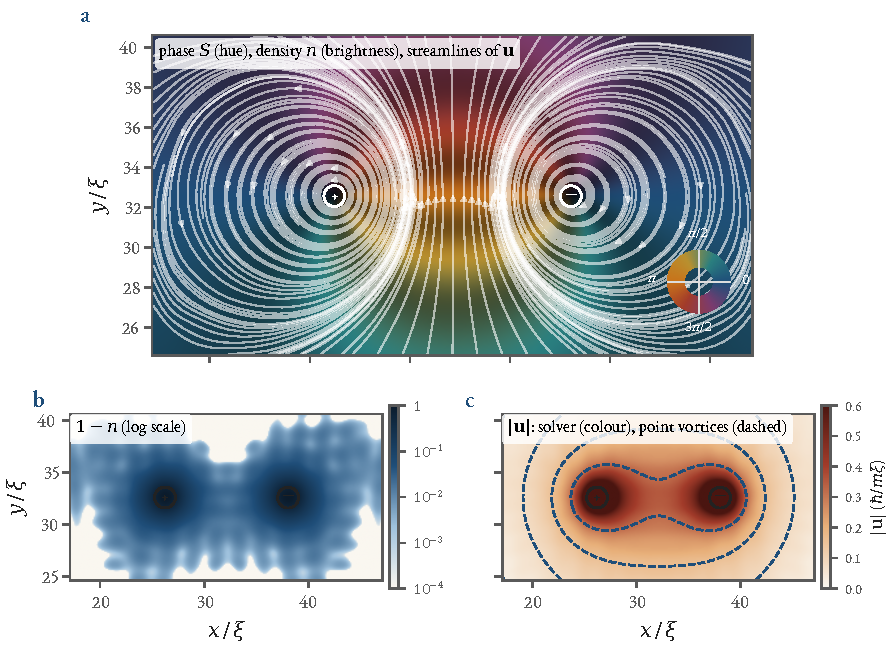
\includegraphics[width=\linewidth]{figures/ch03_phasefield.pdf}
\caption[One wave function, three faces]{One wave function, three faces (qf-pgpe, $t=20$, pair of separation $d\approx12\,\xi$, $+$ vortex on the left). \textbf{(a)}~Phase of $\psi$ (hue; global phase $\ee^{-\ii t}$ removed), density (brightness), streamlines of the Madelung velocity (white). \textbf{(b)}~Density deficit $1-n$, logarithmic; the faint rings are radiated sound. \textbf{(c)}~Speed $|\mathbf u|$: solver (colour) and periodic point vortices with their uniform flow (dashed contours at $0.04,0.08,0.16,0.32$).}
\label{ch03:fig-phasefield}\end{figure}

Three checks make the reading quantitative. First, the grid-level detector finds exactly $\cthreeNum{nPlus}$ plaquette of charge $+1$, $\cthreeNum{nMinus}$ of charge $-1$ and $\cthreeNum{nOther}$ of any other charge, and the same on a grid refined four-fold by spectral interpolation. The positions it reports are within $\cthreeNum{zeroOffset}\,\xi$ of exact zeros of the band-limited field: minimizing $|\psi|^2$ from the detected position finds points where $|\psi|^2\le\cthreeNum{zeroPsiMax}$, so the cores are zeros of $\psi$, as \cref{ch03:zero} requires. The largest principal phase step over all grid edges is $\cthreeNum{maxStepOverPi}\,\pi$ ($\cthreeNum{maxStepRefined}\,\pi$ on the refined grid), so no edge is near the branch point of \cref{ch03:circ}.

Second, panel (c): the relative rms difference between the Madelung velocity of the solver and the periodic point-vortex velocity (with the uniform flow of \cref{ch03:speed}) is $\cthreeNum{velRelInner}\%$ in the shell $1.5$--$3\,\xi$ about the cores and $\cthreeNum{velRelThreeSix}\%$ in the shell $3$--$6\,\xi$; without the uniform flow the second number is $\cthreeNum{velRelThreeSixNoSector}\%$. The phase of one Gross--Pitaevskii vortex is the azimuth exactly, which is why the point-vortex law holds so close to the core; I did not isolate the origin of the remaining two percent. Farther out the difference is $\cthreeNum{velFarRms}$ rms beyond $6\,\xi$, against a point-vortex speed of only $\cthreeNum{velFarPV}$, and it is not vortex flow: $\cthreeNum{curlFree}\%$ of its energy is curl-free and its rms equals that of the density ripple, $\cthreeNum{rmsDn}$ (the sound speed is $1$). It is the sound radiated while the imprinted state relaxes, visible as rings in panel (b) and absent from the point-vortex model.

Third, the first Madelung equation \eqref{ch03:eq-cont}. Evaluating $\partial_tn$ and $\nabla\!\cdot(n\mathbf u)$ with the engine's own right-hand side (no time stepping, no tracking), the continuity equation holds to a relative rms residual of $\cthreeNum{contRel}\%$ of $|\partial_tn|$ outside $3\,\xi$ from the cores. The residual is not noise: for the \emph{projected} equation it equals $-2\operatorname{Im}\big(\bar\psi\,(1-\mathcal P)[|\psi|^2\psi]\big)$, the part of the cubic term that the projector removes, an identity the script checks to $\cthreeNum{projIdentity}$ (largest residual $\cthreeNum{projResidualMax}$). The engine conserves the total norm, not the local continuity equation.

\subsection{Counting quanta}\label{ch03:counting}

Now the quantization of \cref{ch03:circ} on the solver field. Around the $+$ vortex, at its detected position, take circles of radius $R$ from $0.15\,\xi$ to $\cthreeNum{circRmax}\,\xi$ ($\cthreeNum{circLoops}$ loops), evaluate $\psi$ and $\nabla\psi$ at $1600$ points of each circle from the exact mode sum (not the grid), and compute the two quantities that the theory ties together: the circulation integral $\Gamma/\kappa$ with the Madelung velocity, and the winding found by the sum of principal differences of $\arg\psi$.

\begin{rustbox}{two ways to count the quanta}
\lstinputlisting[style=py,basicstyle=\ttfamily\footnotesize,linerange={24-24,26-27}]{figures/ch03_lib.py}
\medskip
\lstinputlisting[style=py,basicstyle=\ttfamily\footnotesize,linerange={48-48,51-53}]{figures/ch03_lib.py}
\medskip
\lstinputlisting[style=py,basicstyle=\ttfamily\footnotesize,linerange={55-55,58-62}]{figures/ch03_lib.py}
\smallskip\footnotesize
Docstrings omitted. \cthreeCode{pdiff} is the numpy form of \Lthm{VortexWinding}{pdiff}; \cthreeCode{ev} evaluates the band-limited field and its gradient at any point from the mode sum.
\end{rustbox}

\begin{figure}[tbp]\centering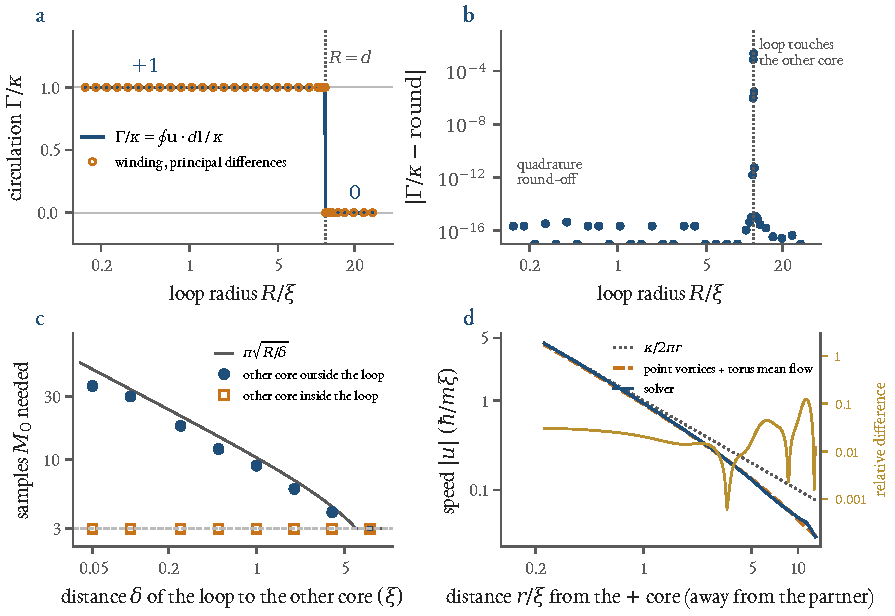
\includegraphics[width=\linewidth]{figures/ch03_circulation.pdf}
\caption[Counting quanta on the solver field]{Counting quanta on the solver field ($d\approx12\,\xi$, $t=20$, circles about the $+$ vortex). \textbf{(a)}~Circulation $\Gamma/\kappa$ (line) and detector winding (circles) against loop radius. \textbf{(b)}~Distance of $\Gamma/\kappa$ from the nearest integer. \textbf{(c)}~Smallest number of samples $M_0$ from which the principal-difference sum is right for every finer sampling, for a loop at distance $\delta$ from the other core, outside (blue) or inside (orange) the loop; worst of six starting angles. \textbf{(d)}~Speed along the line through both cores, on the side of the $+$ vortex away from its partner, against the distance $r$ to the core: solver, periodic point vortices, and $\kappa/2\pi r$ (dotted); gold, right axis: relative difference of the first two.}
\label{ch03:fig-circ}\end{figure}

The result, \cref{ch03:fig-circ}(a,b), is as sharp as the theorem allows. For every loop that encloses only the $+$ vortex ($R$ from $\cthreeNum{circRlo}$ to $\cthreeNum{circRhi}\,\xi$) $\Gamma/\kappa=1$ to within $\cthreeNum{circInnerDev}$; for every loop that encloses both ($R>d+1.4\,\xi$) it is zero to within $\cthreeNum{circOuterDev}$. The circulation of the solver is quantized in units of $\kappa$ to the accuracy of the quadrature, and the pair is invisible from outside, as \Lthm{ScaleResolvedWinding}{dipole_invisible} says it must be. The step from $1$ to $0$ takes place across the other core, where what limits the numbers is the quadrature and not the quantization: within $0.2\,\xi$ of that core the integrand is sharply peaked and $1600$ points no longer resolve it ($|\Gamma/\kappa-\text{integer}|=\cthreeNum{devDelta02}$, $\cthreeNum{devDelta01}$ and $\cthreeNum{devDelta005}$ at distances $0.2$, $0.1$ and $0.05\,\xi$). The detector, which only compares phases at consecutive samples, returns the right integer on all $\cthreeNum{circLoops}$ loops, including those three.

Panel (c) answers the question that \Lthm{ContinuumWinding}{detector_correct} leaves open: how large is $n_0$? Sample a circle with $M$ equally spaced points, for every divisor $M$ of $\cthreeNum{n0Mmax}$ and from one of six generic starting angles, and ask for the smallest $M_0$ from which every finer sampling gives the right winding; the worst of the six angles is plotted. A bare vortex needs $M_0=3$, since its step $2\pi/M$ must stay below $\pi$. If the other core lies \emph{inside} the loop, $M_0$ stays at $\cthreeNum{n0InMax}$ at every distance tested, down to $\delta=\cthreeNum{n0DeltaNear}\,\xi$. If it lies \emph{outside}, $M_0$ grows as the loop approaches it, from $\cthreeNum{n0OutFar}$ at $\delta=\cthreeNum{n0DeltaFar}\,\xi$ to $\cthreeNum{n0OutNear}$ at $\delta=\cthreeNum{n0DeltaNear}\,\xi$, as $\delta^{\cthreeNum{n0OutExp}}$. The reading is the hypothesis of the Lean theorems in quantitative form: the detector goes wrong exactly when the \emph{true} phase change between neighbouring samples reaches $\pi$. Along an arc of length $\ell=2\pi R/M$ passing a zero at distance $\delta$, the phase of that zero changes by up to $\pi-4\delta/\ell$, adding to the loop's own step $2\pi/M$ if the zero has the opposite charge and lies outside the loop, and subtracting from it if the zero lies inside. The sum reaches $\pi$ once $M\lesssim\pi\sqrt{R/\delta}$, and the measured $M_0$ are $\cthreeNum{n0RatioLo}$ to $\cthreeNum{n0RatioHi}$ times that. This derivation is mine, checked against these numbers, and is not in the library. So $n_0$ is finite, as the theorem says, but not a number the theorem could know: it depends on the distance to the nearest zero of $\psi$ and on whether that zero helps or opposes the winding being measured.

\paragraph{The torus has its own windings.} A loop does not have to be contractible. On the periodic grid the sums of principal differences along each of the $128$ rows and $128$ columns are again integers (to $\cthreeNum{torusDev}$), by the same theorem: all row windings are $0$, and the column windings are $1$ for the $\cthreeNum{nColsNonzero}$ columns between the two vortices and $0$ elsewhere. The integer pair measured outside that strip is the \emph{sector} of the state. The circulation of $\mathbf u$ around a cycle of the torus is $2\pi$ times it, so the \emph{mean} velocity over the box is fixed by the sector and the vortex positions, not by dynamics. For this pair the column windings give $\langle u_y\rangle=2\pi\,(\cthreeNum{nColsNonzero}\times0.5\,\xi)/L^2=\cthreeNum{ubarWinding}$, the integral of the Madelung velocity over the grid gives $\cthreeNum{ubarBox}$, and the position formula of \cref{ch03:speed} gives $\cthreeNum{ubarFormula}$; they agree to the width of one grid column. This small uniform flow has a large effect.

\subsection{Where the energy sits}\label{ch03:energy}

The identity of \Lthm{MadelungSplit}{kinetic_density_split} can be evaluated on the field: split $\frac12|\nabla\psi|^2$ at every point into $\frac12|\nabla\sqrt n|^2$ and $\frac12n|\mathbf u|^2$, on the refined $512^2$ grid, and integrate. The pointwise difference between the kinetic density and the sum of the two parts is $\cthreeNum{pointwiseErr}$ of its maximum (on the solver grid itself, $\cthreeNum{pointwiseErrCoarse}$): an algebraic identity holding to rounding error, not a measurement. What is measured is the partition. The integral of $\frac12|\nabla\psi|^2$ is $\cthreeNum{eKin}$ in units of $\hbar^2n_0/m$ (the Parseval sum of the Fourier amplitudes gives $\cthreeNum{eKinParseval}$); of this, $\cthreeNum{eFlow}$ ($\cthreeNum{fracFlow}\%$) is flow and $\cthreeNum{eQ}$ ($\cthreeNum{fracQ}\%$) is quantum pressure. The total energy of the pair above the uniform state is $\cthreeNum{eExcess}$; the remainder, $\frac12\int(n-1)^2\,\dd^2x$, is the interaction energy of the density disturbance.

\begin{figure}[tbp]\centering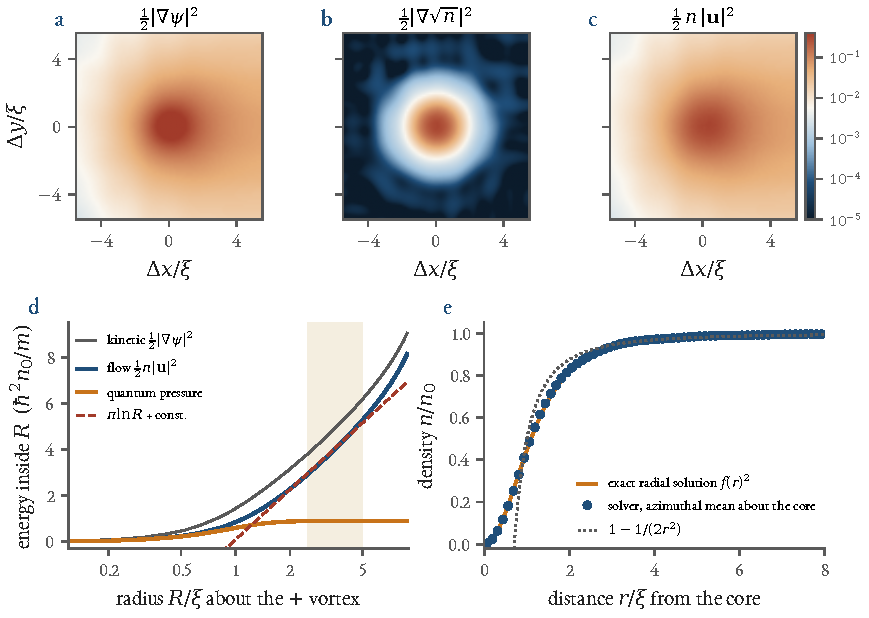
\includegraphics[width=\linewidth]{figures/ch03_energy.pdf}
\caption[Where the energy of a vortex sits]{Where the energy of a vortex sits ($d\approx12\,\xi$, $t=20$, refined grid). \textbf{(a--c)}~Kinetic, quantum-pressure and flow energy density near the $+$ vortex, one logarithmic scale. \textbf{(d)}~Energy inside radius $R$ about the core: the flow part follows $\pi\ln R$ in the shaded window and keeps growing, the quantum-pressure part saturates inside $3\,\xi$. \textbf{(e)}~Azimuthal mean density against the exact radial solution of \eqref{ch03:eq-profile}.}
\label{ch03:fig-energy}\end{figure}

\Cref{ch03:fig-energy} shows where the two parts live. The quantum pressure is a ring around the core: inside $3\,\xi$ it holds $\cthreeNum{qWithinThree}$ and inside $6\,\xi$ $\cthreeNum{qWithinSix}$, so it has saturated, whereas the flow energy inside the same radii is $\cthreeNum{flowWithinThree}$ and $\cthreeNum{flowWithinSix}$ and keeps growing. Fitting the flow energy against $\ln R$ for $2.5\le R/\xi\le5$ gives a slope of $\cthreeNum{slopePlus}$ about the $+$ vortex and $\cthreeNum{slopeMinus}$ about the $-$ vortex. The vortex's own azimuthal flow $\hbar/(mr)$ contributes $\cthreeNum{slopeSelf}$, to be compared with $\pi\bar n=\cthreeNum{slopePredicted}$ for the measured mean density $\bar n=\cthreeNum{nbarR}$ on the circle $R=3.75\,\xi$; the partner's flow and the uniform flow inside the disc contribute $\cthreeNum{slopePartner}$, the cross term $\cthreeNum{slopeCross}$, and the three add up to the measured slope. Panel (e) puts the core against its exact profile: they differ by at most $\cthreeNum{profMaxDiff}$ in density over $r\le8\,\xi$ ($n(1\,\xi)=\cthreeNum{nAtR1Solver}$ against $\cthreeNum{nAtR1Exact}$). I did not isolate the origin of this one-percent difference.

\subsection{The speed of a pair, and the lesson of the periodic box}\label{ch03:speed}

The Lean module of \cref{ch03:pair} says that a point-vortex pair of separation $d$ moves at $\hbar/(md)$. Does the Gross--Pitaevskii pair in a periodic box of side $64\,\xi$ do so? The solver was run for six separations, $d=4,6,8,12,16,20\,\xi$ (40 time units each; $d=12\,\xi$ is the run of the previous figures); the speed is the slope of the position of the pair's centre over $10\le t\le40$, the first ten time units containing the relaxation of the imprint. Three predictions can be made, each with one more ingredient than the last.

\begin{enumerate}
\item \emph{The plane law}, $v=\hbar/(md)$.
\item \emph{Point vortices on the torus.} Each vortex is carried by the velocity of the other and of all its periodic images. In Fourier space the velocity of vortices of charges $q_j$ at $\mathbf x_j$ is $\hat{\mathbf u}(\mathbf k)=\ii\,(k_y,-k_x)\,\hat\rho(\mathbf k)/|\mathbf k|^2$ with $\hat\rho(\mathbf k)=(\kappa/L^2)\sum_jq_j\ee^{-\ii\mathbf k\cdot\mathbf x_j}$, and the term $\mathbf k=0$ is absent: this is the field with \emph{zero mean flow}. The programme's earlier code has the same field in closed form (the Weiss--McWilliams pair function); the two agree to $\cthreeNum{fourierDiff}$ on the test configuration of the box below.
\item \emph{Plus the uniform flow that the windings of the torus force.} With positions taken in $[0,L)$, the circulation of the zero-mean-flow field around the $x$-cycle just above the line $y=0$ is $-(\kappa/L)\sum_jq_jy_j$, and around the $y$-cycle just above $x=0$ it is $+(\kappa/L)\sum_jq_jx_j$, which are not integer multiples of $\kappa$. The wave function requires $2\pi$ times an integer, and the integers measured in \cref{ch03:counting} are zero, so a uniform flow must make up the difference:
\begin{equation}\label{ch03:eq-ubar}
  \bar{\mathbf u}=\frac{\kappa}{L^2}\Big(\sum_jq_jy_j,\;-\sum_jq_jx_j\Big).
\end{equation}
For a pair of separation $d$ it has magnitude $\kappa d/L^2$ and the direction of the pair's own motion; it is the impulse of the pair divided by $mn_0L^2$. In units of the plane speed it is $\bar u/(\hbar/md)=2\pi d^2/L^2$, that is $\cthreeNum{ubarOverV}\%$ at $d=12\,\xi$ and $\cthreeNum{ubarOverV20}\%$ at $d=20\,\xi$.
\end{enumerate}

\begin{rustbox}{the periodic point-vortex model}
\lstinputlisting[style=py,basicstyle=\ttfamily\footnotesize,firstline=29,lastline=31]{figures/ch03_pv.py}
\medskip
\lstinputlisting[style=py,basicstyle=\ttfamily\footnotesize,linerange={68-68,70-74}]{figures/ch03_pv.py}
\smallskip\footnotesize
\texttt{pv\_velocity} is the programme's zero-mean-flow field (\texttt{exploration/pgpe/transport\_estimators.py}); the Fourier-series version \cthreeCode{fourier_velocity} of \texttt{figures/ch03\_pv.py} agrees with it to $\cthreeNum{fourierDiff}$ on a test configuration ($+$ at $(26.30,30.70)$, $-$ at $(38.10,31.20)$; recorded in \texttt{ch03\_numbers.json}).
\end{rustbox}

\begin{figure}[tbp]\centering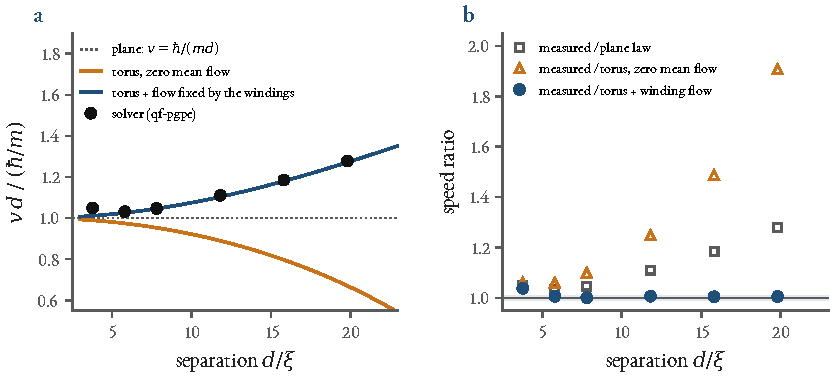
\includegraphics[width=\linewidth]{figures/ch03_pairspeed.pdf}
\caption[The speed of a vortex pair in the periodic box]{The speed of a vortex pair in the periodic box against its separation (six solver runs of 40 time units). \textbf{(a)}~$v\,d/(\hbar/m)$: the plane law ($=1$), point vortices on the torus with zero mean flow (orange), the same plus the uniform flow \eqref{ch03:eq-ubar} fixed by the windings (blue), and the measurements (black). \textbf{(b)}~Ratio of the measured speed to each prediction; the band is $\pm1\%$.}
\label{ch03:fig-speed}\end{figure}

\begin{table}[tbp]\centering\small
\begin{tabular}{@{}rccccccc@{}}
\toprule
$d/\xi$ & measured & plane & torus, & torus $+$ & \multicolumn{3}{c}{measured $/$}\\
 & & $1/d$ & zero flow & winding flow & plane & zero flow & $+$ flow\\
\midrule
3.8 & 0.2778 & 0.2648 & 0.2619 & 0.2677 & 1.049 & 1.061 & 1.038\\
5.8 & 0.1781 & 0.1726 & 0.1681 & 0.1770 & 1.032 & 1.059 & 1.006\\
7.8 & 0.1342 & 0.1282 & 0.1221 & 0.1341 & 1.047 & 1.099 & 1.001\\
11.8 & 0.0940 & 0.0847 & 0.0753 & 0.0934 & 1.110 & 1.249 & 1.006\\
15.8 & 0.0750 & 0.0633 & 0.0504 & 0.0746 & 1.185 & 1.488 & 1.005\\
19.8 & 0.0645 & 0.0505 & 0.0338 & 0.0642 & 1.278 & 1.908 & 1.005\\
\bottomrule
\end{tabular}

\caption{The measured speed of the pair against the three predictions (units $\hbar/m\xi$ per unit time; $d$ is the separation averaged over $10\le t\le40$; the predictions are evaluated at the tracked positions and averaged over the same window).}
\label{ch03:tab-speed}\end{table}

\Cref{ch03:fig-speed} and \cref{ch03:tab-speed} give the result. The measured speed exceeds the plane law by $\cthreeNum{pctPlaneMin}$ to $\cthreeNum{pctPlane8}\%$ for $d\le8\,\xi$ and by $\cthreeNum{pctPlane12}\%$, $\cthreeNum{pctPlane16}\%$ and $\cthreeNum{pctPlane20}\%$ at $d=12,16,20\,\xi$. The torus point-vortex speed with zero mean flow is too small, and increasingly so with $d$: the measured speed is $\cthreeNum{scanTwelveRatioPvz}$, $\cthreeNum{scanSixteenRatioPvz}$ and $\cthreeNum{scanTwentyRatioPvz}$ times it at $d=12,16,20\,\xi$, so the discrepancy is not a core effect, which would shrink with $d$. With the uniform flow \eqref{ch03:eq-ubar} the ratios are $\cthreeNum{scanSixRatioPv}$, $\cthreeNum{scanEightRatioPv}$, $\cthreeNum{scanTwelveRatioPv}$, $\cthreeNum{scanSixteenRatioPv}$ and $\cthreeNum{scanTwentyRatioPv}$ for $d\ge6\,\xi$: the prediction reproduces the solver to about one percent, with no fitted parameter. At $d\approx4\,\xi$ the measured speed is $\cthreeNum{pctPvFour}\%$ above it; there the pair is a solitary wave of the compressible field rather than two point vortices \cite{JonesRoberts1982}. That is the sign and size of the discrepancy, not a derivation of it.

The same effect appeared in the programme's study of friction on vortices, where it was first misread: the ratios of the box-frame speed to the zero-mean-flow prediction there ($1.06,1.06,1.10$ and $1.49$ at $d=4,6,8$ and $16\,\xi$, in its table of $T=0$ kinematics \cite{Callens2026a}; different runs and imprint position) are the numbers measured here. The lesson is general. A vortex pair carries impulse, and a periodic box has no infinity to which to assign it, so the fluid as a whole moves; the amount is a property not of the dynamics but of the integers that wind the phase around the torus, whose existence \Lthm{VortexWinding}{loop_sum_eq_mul} guarantees.

The field momentum is conserved ($P_y=\cthreeNum{momPy}$, relative change $\cthreeNum{momDrift}$) but is $\cthreeNum{momRatio}\%$ of the impulse $2\pi d=\cthreeNum{momImpulse}$ at $t=20$. The difference is the density deficit: the momentum is $\int n\,u_y\,\dd^2x$, and the integral of $u_y$ alone over the box, $L^2\times\cthreeNum{ubarBox}$, exceeds it by $\int(1-n)\,u_y\,\dd^2x$, which is $\cthreeNum{momDeficitPct}\%$ of it. The separation shrinks by $\cthreeNum{dipoleMomRelShrink}\%$ over the run, so the impulse of the vortices falls while the field momentum does not; the balance must be carried by the sound field.

\subsection{Leapfrogging pairs, and the reduced model in CVODE}\label{ch03:leap}

\begin{figure}[tbp]\centering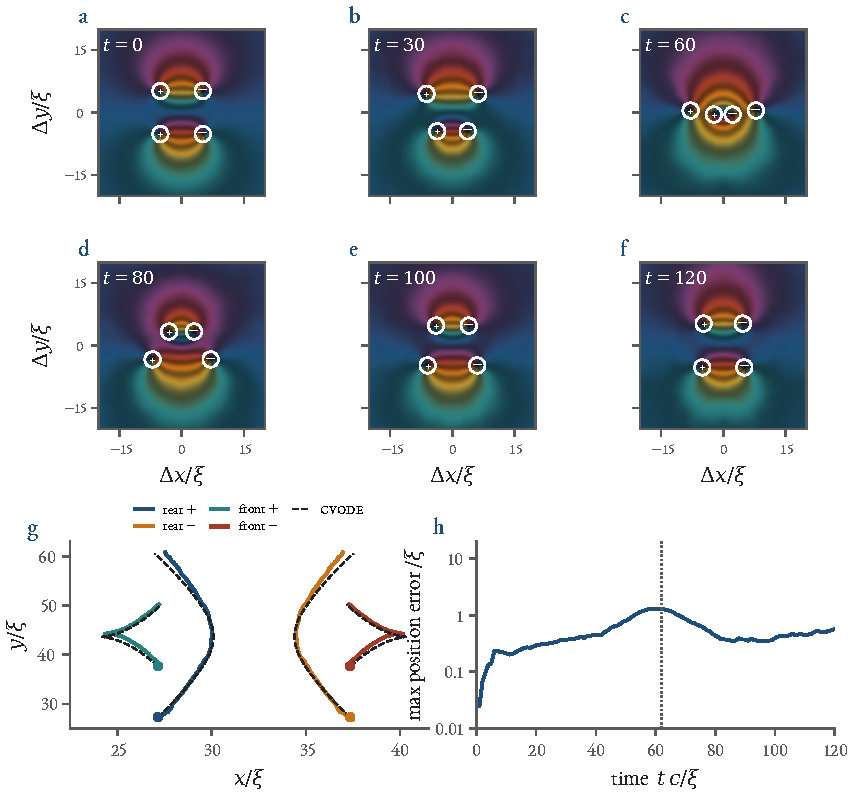
\includegraphics[width=\linewidth]{figures/ch03_leapfrog.pdf}
\caption[Two vortex pairs leapfrog]{Two vortex pairs leapfrog (qf-pgpe, $L=64\,\xi$, 120 time units). \textbf{(a--f)}~The wave function at six times (colour code of \cref{ch03:fig-phasefield}), the view re-centred on the four vortices. \textbf{(g)}~Tracked vortices (solid) and the periodic point-vortex model integrated with CVODE (dashed) from the detected positions at $t=0$ (dots). \textbf{(h)}~Largest distance between a tracked vortex and its model trajectory; dotted: the time at which the rear pair passes the front pair in the solver.}
\label{ch03:fig-leap}\end{figure}

Two pairs of the same sense, one behind the other, give a motion familiar from classical hydrodynamics as the leapfrogging of vortex rings. The rear pair is drawn forward by the flow of the front pair, narrows as it accelerates, passes through the front pair, which has widened and slowed, and then widens in its turn while the other narrows. The solver was started with four vortices $+,-,+,-$ at the corners of a square of side $10.3\,\xi$ and run for $\cthreeNum{quadT}$ time units; \cref{ch03:fig-leap} shows the wave function at six times and the tracked vortices.

The reduced model is the periodic point-vortex model of \cref{ch03:speed}: four vortices obeying $\dot{\mathbf x}_a=\mathbf u_a(\mathbf x)+\bar{\mathbf u}$, with $\mathbf u_a$ the zero-mean-flow field of the other three and their images and $\bar{\mathbf u}$ the uniform flow \eqref{ch03:eq-ubar}, constant here because $\sum_jq_j\mathbf x_j$ is conserved. It is integrated with CVODE from the positions detected at $t=0$.

\begin{rustbox}{CVODE integrates the point-vortex model}
\lstinputlisting[style=py,basicstyle=\ttfamily\footnotesize,firstline=83,lastline=85]{figures/ch03_pv.py}
\medskip
\lstinputlisting[style=py,basicstyle=\ttfamily\footnotesize,firstline=87,lastline=92]{figures/ch03_pv.py}
\smallskip\footnotesize
Excerpt of \cthreeCode{integrate_cvode} (\texttt{figures/ch03\_pv.py}; \texttt{rhs} advances the state, the loop restarts CVODE at each output time). Run with the rusty-SUNDIALS build of commit \texttt{5db8041}, \texttt{rusty\_sundials.\_\_file\_\_} recorded in \texttt{ch03\_numbers.json}. Result for the four-vortex run: \cthreeNum{cvodeCalls} right-hand-side calls in \cthreeNum{cvodeSeconds}~s for 120 time units on the loaded machine (the right-hand side is a Python function called through the binding); an independent integration of the same equations with SciPy's DOP853 at tolerance $10^{-12}$ differs from the CVODE trajectory by at most $\cthreeNum{cvodeVsDop}\,\xi$ over the whole run, and the dipole moment $\sum_jq_j\mathbf x_j$, conserved by the equations, is conserved by CVODE to $\cthreeNum{cvodeDipole}$.
\end{rustbox}

Against the solver the model does well, and one cause of the difference can be measured. The rear pair narrows from $\cthreeNum{quadWidth0}\,\xi$ to $\cthreeNum{quadRearMin}\,\xi$ in the solver ($\cthreeNum{quadRearMinODE}\,\xi$ in the model) and the front pair widens to $\cthreeNum{quadFrontMax}\,\xi$ ($\cthreeNum{quadFrontMaxODE}\,\xi$); the rear pair passes the front pair at $t=\cthreeNum{passGP}$ in the solver and at $t=\cthreeNum{passODE}$ in the model, $\cthreeNum{passDiff}$ time units ($\cthreeNum{passDiffPct}\%$) earlier; by $t=\cthreeNum{quadT}$ the roles are exchanged, the former rear pair being $\cthreeNum{quadYLead}\,\xi$ ahead in the solver. The largest distance between a tracked vortex and its model trajectory is $\cthreeNum{quadErr10}$, $\cthreeNum{quadErr20}$ and $\cthreeNum{quadErr40}\,\xi$ at $t=10,20,40$, rises to $\cthreeNum{quadErr60}\,\xi$ at the passage, where a small error in timing becomes a large error in position because the vortices move fastest, and is $\cthreeNum{quadErr100}$ and $\cthreeNum{quadErr120}\,\xi$ at $t=100,120$.

Where does the difference come from? Part of it is the imprint: the imprinted state relaxes, and the error is already $0.22\,\xi$ at $t=8$. Restarting the model from the tracked positions at a later time tests this (with DOP853, which takes seconds). Started at $t=0,10,20,40$ the model passes the front pair at $t=\cthreeNum{restartPass0},\cthreeNum{restartPass10},\cthreeNum{restartPass20},\cthreeNum{restartPass40}$ against $\cthreeNum{passGP}$ in the solver, and its largest error over the rest of the run is $\cthreeNum{restartErrMax0},\cthreeNum{restartErrMax10},\cthreeNum{restartErrMax20},\cthreeNum{restartErrMax40}\,\xi$; ten time units after a restart at $t=20$ it is $\cthreeNum{restartErrTen20}\,\xi$. So most of the passing-time discrepancy is the first twenty to forty time units of relaxation, not an inability of point vortices to leapfrog. What is left (a restart at $t=40$: $0.4\,\xi$ at worst, a passing time within $0.5$ time units) is what point vortices lack, the core structure and the compressibility of the field; I did not separate the two. The closest approach inside a pair is $\cthreeNum{quadMinSepGP}\,\xi$, where the speed excess of the previous subsection lies between $\cthreeNum{scanSixPctPv}\%$ and $\cthreeNum{pctPvFour}\%$. The impulse $\sum_jq_j\mathbf x_j$ is conserved exactly in the model and falls by $\cthreeNum{quadDipoleChange}\%$ over the run in the solver, while the total field momentum is conserved to $\cthreeNum{quadMomDrift}$ and the energy to $\cthreeNum{quadEnergyDrift}$.

\section{What this chapter establishes, and what it does not}\label{ch03:honest}

\begin{honestbox}
\textbf{Proved in Lean} (standard axioms \texttt{propext}, \texttt{Classical.choice}, \texttt{Quot.sound}: by the programme's compile audit for \texttt{VortexWinding}, \texttt{MadelungSplit} and \texttt{MadelungNSE}; re-compiled for this chapter for \texttt{QuantizedCirculation}, \texttt{ContinuumWinding} and \texttt{ScaleResolvedWinding}). Sums of principal phase differences around a closed loop are integer multiples of $2\pi$, so the discrete circulation is $q\kappa$, a nonzero one has $|\Gamma|\ge\kappa$, and $\kappa$ is attained; for a continuous nowhere-vanishing closed loop the detector returns $2\pi w$ for every fine enough sampling, $n_0$ unquantified; the kinetic energy density of $a\,\ee^{\ii S}$ splits into an amplitude and a phase term; $\operatorname{div}\mathbf u=(\hbar/m)\Delta S$ in a Navier--Stokes vocabulary; a dipole is invisible to the discrete winding of any enclosing region. \emph{New here} (\texttt{book/lean/Ch03\_PointVortexPair.lean}, zero errors, same three axioms): the point-vortex law implies that a $\pm\Gamma$ pair translates rigidly at $\hbar/(md)$ for $\Gamma=\kappa$, at constant separation.

\textbf{Not in Lean}, and textbook: the Madelung equations; the vortex profile \eqref{ch03:eq-profile}; the energy and impulse of a pair and $U=\mathrm dE/\mathrm dP$; that a Gross--Pitaevskii vortex moves with the velocity induced by the others; that a nonzero winding implies a zero of $\psi$ inside.

\textbf{Simulated} (qf-pgpe at $128^2$, $k_{\rm cut}=\pi/\xi$, zero temperature, one initial condition per case, up to $120$ time units; CVODE for the reduced model). Circulation is an integer to $\cthreeNum{circInnerDev}$ and the detector is right on all $\cthreeNum{circLoops}$ loops; $\cthreeNum{fracFlow}\%$ of the kinetic energy of the pair is flow; the pair speed equals the torus point-vortex prediction with the winding-fixed flow to about $1\%$ for $d\ge6\,\xi$ ($\cthreeNum{pctPvFour}\%$ above it at $d\approx4\,\xi$); the model follows the leapfrog to $\cthreeNum{quadErrMax}\,\xi$ at worst over $120$ time units, with a $\cthreeNum{passDiffPct}\%$ error in the passing time, mostly the relaxation of the imprint.

\textbf{Analogy only.} The Madelung equations have the form of those of a classical inviscid fluid, and vortex pairs in the quantum fluid move like pairs in the classical one. LL-15: what the two systems must share for this to transfer is a velocity that is a gradient away from a few singular points that the flow carries; the quantum fluid adds the single-valuedness of $\psi$ (quantized circulation, no continuous vorticity), the point-vortex model lacks the compressibility of the field. Nothing here is a prediction for the liquid helium of \cref{ch03:obs}: Gross--Pitaevskii is a model of it.

\textbf{What failed or was wrong on the way.} (i) The first compilation of the new Lean file failed on three proofs (a simplifier normal form for the conjugate of a difference, an unsolved imaginary part, the same form inside a norm); the version shown is the one that compiled. (ii) My first guess for the sampling threshold $n_0$ (the number of samples needed to resolve a $\pi$ step across the distance to the other core) was wrong twice over: loops started towards that core needed no extra samples, and with generic starting angles the threshold depends on whether the other zero is inside or outside the loop and grows as $\delta^{-1/2}$. (iii) In the programme's friction study the excess of the measured pair speed over the zero-mean-flow prediction (up to $49\%$) was first read as an imprint transient; it is the uniform flow of the torus (CLAIM-082 of the programme's ledger). (iv) The first CVODE run of the reduced model used a stale build of the Python module, older than the repair of commit \texttt{5db8041} of rusty-SUNDIALS: it needed $\cthreeNum{staleCalls}$ right-hand-side calls and differed from DOP853 by $\cthreeNum{staleVsDop}\,\xi$, against $\cthreeNum{cvodeCalls}$ calls and $\cthreeNum{cvodeVsDop}\,\xi$ for the repaired build, with which the run was redone.
\end{honestbox}

\section*{Exercises}\label{ch03:ex}
\addcontentsline{toc}{section}{Exercises}

\paragraph{Exercise 1.} \emph{Two samples are not enough.} A vortex has phase $\theta(\varphi)=\varphi$ along a circle centred on it. (a) For $n=2$ samples, at $\varphi=0$ and $\pi$, compute the sum of principal differences for the counter-clockwise and for the clockwise traversal. (b) Explain with \Lthm{VortexWinding}{pdiff_add_rev_eq_two_pi_iff} why both give the same answer, and why \Lthm{ContinuumWinding}{detector_correct} says nothing about this sampling. (c) For which $n$ is the sum right for every starting angle? \emph{Hint:} the principal value of a step of exactly $\pi$ is $+\pi$ in both directions; for (c) all steps $2\pi/n$ must be below $\pi$.

\paragraph{Exercise 2.} \emph{The mean flow of the torus.} (a) Show from \eqref{ch03:eq-ubar} that $\bar u/(\hbar/md)=2\pi d^2/L^2$ and evaluate it for $d=6,12,16\,\xi$, $L=64\,\xi$. (b) Derive \eqref{ch03:eq-ubar} for one pair, the $+$ vortex at $(x_1,y)$ and the $-$ vortex at $(x_2,y)$. \emph{Hint:} the circulation of the zero-mean-flow field around a row $y=\text{const}$ is piecewise constant in $y$ (it changes by $\mp\kappa$ across a vortex), has zero mean over $y$, and the wave function requires an integer multiple of $2\pi$. (c) In which direction, and how fast, does the pair with the $+$ vortex \emph{below} the $-$ vortex, at the same $x$, move? \emph{Hint:} the box has fourfold symmetry; check the direction with \cthreeCode{vortex_velocity}.

\paragraph{Exercise 3.} \emph{Run it.} With \texttt{qf\_pgpe}, imprint the pair of \cref{ch03:engine} with $d=12\,\xi$ in a box of side $L=96\,\xi$ with $192^2$ grid points (the same $\Delta x$), run for $40$ time units and measure the speed as in \cref{ch03:speed}. Predict it first from \eqref{ch03:eq-ubar} and the zero-mean-flow field (\cthreeCode{vortex_velocity} with \texttt{L=96}); what changes between the two boxes, and by how much? \emph{Hint:} the uniform flow scales as $L^{-2}$, and so, to leading order, does the correction from the images. For comparison, my run of this recipe (\cthreeNum{exWall}~s on the loaded machine) gave $v=\cthreeNum{exVmeas}$ against the prediction $\cthreeNum{exVpv}$, where the same pair in the $64\,\xi$ box moves at $\cthreeNum{scanTwelveMeas}$.

\section*{Notes and further reading}
\addcontentsline{toc}{section}{Notes and further reading}

The hydrodynamic form of the Schr\"odinger equation is Madelung's \cite{Madelung1927}; the quantization of circulation was proposed by Onsager \cite{Onsager1949} and applied by Feynman to rotating helium \cite{Feynman1955}. It was detected in single quanta in Vinen's vibrating-wire experiment \cite{Vinen1961} (Zieve's retrospective \cite{Zieve2023} is a good entry point) and the arrays of lines were photographed by Yarmchuk, Gordon and Packard \cite{Yarmchuk1979}. For the Gross--Pitaevskii vortex see \cite{Gross1961,Pitaevskii1961} and the books of Pitaevskii and Stringari \cite{PitaevskiiStringari2016} and, for the liquid, Donnelly \cite{Donnelly1991}; vortices are carried by the flow of the others in Helmholtz's analysis \cite{Helmholtz1858}, and the pair as a solitary wave of the compressible field is the subject of Jones and Roberts \cite{JonesRoberts1982}. The projected method is reviewed in \cite{Blakie2008}; the engine is \cite{Callens2026sw}, the library \cite{Callens2026lib}, and the friction study that identified the mean flow of the torus \cite{Callens2026a}. The pairs of this chapter are what unbinds in \cref{ch06}, what moves with dissipation in \cref{ch07}, and what a moving obstacle sheds in \cref{ch09}, in the simulations of Kwon and Shin \cite{KwonShin2026prr}.

\setlength{\emergencystretch}{\cthreeOldES}
\let\topfraction\cthreeOldTopFrac\let\textfraction\cthreeOldTextFrac\let\floatpagefraction\cthreeOldFloatFrac
}
\IfCh{ch04}{\chapter{The Specific Heat of Helium-4 and Godfrin's Series}\label{ch04}
% generated by figures/ch04_numbers_tex.py from figures/ch04_numbers.json -- do not edit
\makeatletter
\providecommand{\cfv}[1]{\ifcsname cfv@#1\endcsname\csname cfv@#1\endcsname\else\PackageError{ch04}{Undefined number key #1}{Run ch04_numbers_tex.py}\fi}
\expandafter\gdef\csname cfv@A-pr\endcsname{\ensuremath{0.0831}}
\expandafter\gdef\csname cfv@A-val\endcsname{\ensuremath{0.083091}}
\expandafter\gdef\csname cfv@C-pr\endcsname{\ensuremath{-0.0548}}
\expandafter\gdef\csname cfv@C-val\endcsname{\ensuremath{-0.054809}}
\expandafter\gdef\csname cfv@D-pr\endcsname{\ensuremath{0.0653}}
\expandafter\gdef\csname cfv@D-val\endcsname{\ensuremath{0.065345}}
\expandafter\gdef\csname cfv@E-pr\endcsname{\ensuremath{0.0603}}
\expandafter\gdef\csname cfv@E-val\endcsname{\ensuremath{0.060370}}
\expandafter\gdef\csname cfv@K-pr\endcsname{\ensuremath{-0.262}}
\expandafter\gdef\csname cfv@K-val\endcsname{\ensuremath{-0.26247}}
\expandafter\gdef\csname cfv@L-pr\endcsname{\ensuremath{0.141}}
\expandafter\gdef\csname cfv@L-val\endcsname{\ensuremath{0.14086}}
\expandafter\gdef\csname cfv@T-cross\endcsname{0.77}
\expandafter\gdef\csname cfv@Trange-hi-A\endcsname{0.0543}
\expandafter\gdef\csname cfv@Trange-hi-AC\endcsname{0.0543}
\expandafter\gdef\csname cfv@Trange-hi-ACD\endcsname{0.0543}
\expandafter\gdef\csname cfv@Trange-hi-ACDE\endcsname{0.0543}
\expandafter\gdef\csname cfv@Trange-hi-ACDEK\endcsname{0.0543}
\expandafter\gdef\csname cfv@Trange-hi-ACDEKL\endcsname{0.0543}
\expandafter\gdef\csname cfv@Trange-lo-A\endcsname{0.005}
\expandafter\gdef\csname cfv@Trange-lo-AC\endcsname{0.005}
\expandafter\gdef\csname cfv@Trange-lo-ACD\endcsname{0.005}
\expandafter\gdef\csname cfv@Trange-lo-ACDE\endcsname{0.00849}
\expandafter\gdef\csname cfv@Trange-lo-ACDEK\endcsname{0.0144}
\expandafter\gdef\csname cfv@Trange-lo-ACDEKL\endcsname{0.0188}
\expandafter\gdef\csname cfv@V\endcsname{27.5793}
\expandafter\gdef\csname cfv@a2\endcsname{1.55}
\expandafter\gdef\csname cfv@a3\endcsname{-4.04}
\expandafter\gdef\csname cfv@a4\endcsname{2.30}
\expandafter\gdef\csname cfv@best-err-0.2\endcsname{\ensuremath{2.8\times10^{-7}}}
\expandafter\gdef\csname cfv@best-err-0.3\endcsname{\ensuremath{1.3\times10^{-4}}}
\expandafter\gdef\csname cfv@best-err-0.5\endcsname{\ensuremath{7.6\times10^{-3}}}
\expandafter\gdef\csname cfv@best-err-0.8\endcsname{\ensuremath{9.1\times10^{-2}}}
\expandafter\gdef\csname cfv@best-order-0.2\endcsname{19}
\expandafter\gdef\csname cfv@best-order-0.3\endcsname{19}
\expandafter\gdef\csname cfv@best-order-0.5\endcsname{6}
\expandafter\gdef\csname cfv@best-order-0.8\endcsname{6}
\expandafter\gdef\csname cfv@bose-XEND\endcsname{80}
\expandafter\gdef\csname cfv@bose-calls-1m10\endcsname{688}
\expandafter\gdef\csname cfv@bose-calls-1m12\endcsname{848}
\expandafter\gdef\csname cfv@bose-calls-1m4\endcsname{231}
\expandafter\gdef\csname cfv@bose-calls-1m6\endcsname{383}
\expandafter\gdef\csname cfv@bose-calls-1m8\endcsname{528}
\expandafter\gdef\csname cfv@bose-err-1m10\endcsname{\ensuremath{3.3\times10^{-9}}}
\expandafter\gdef\csname cfv@bose-err-1m12\endcsname{\ensuremath{2.4\times10^{-11}}}
\expandafter\gdef\csname cfv@bose-err-1m4\endcsname{\ensuremath{5.1\times10^{-4}}}
\expandafter\gdef\csname cfv@bose-err-1m6\endcsname{\ensuremath{2.4\times10^{-5}}}
\expandafter\gdef\csname cfv@bose-err-1m8\endcsname{\ensuremath{2.0\times10^{-7}}}
\expandafter\gdef\csname cfv@bose-quad\endcsname{\ensuremath{1\times10^{-16}}}
\expandafter\gdef\csname cfv@bose-ratio-max\endcsname{33}
\expandafter\gdef\csname cfv@bose-ratio-min\endcsname{5.1}
\expandafter\gdef\csname cfv@bud-first_T_series6_vs_measured_ph_exceeds_1pct\endcsname{0.45}
\expandafter\gdef\csname cfv@bud-first_T_series6_vs_poly_exceeds_0p1pct\endcsname{0.30}
\expandafter\gdef\csname cfv@bud-first_T_series6_vs_poly_exceeds_1pct\endcsname{0.45}
\expandafter\gdef\csname cfv@bud-model-0.3\endcsname{\ensuremath{6.0\times10^{-4}}}
\expandafter\gdef\csname cfv@bud-model-0.4\endcsname{\ensuremath{9.8\times10^{-4}}}
\expandafter\gdef\csname cfv@bud-model-0.5\endcsname{\ensuremath{1.4\times10^{-3}}}
\expandafter\gdef\csname cfv@bud-model-0.6\endcsname{\ensuremath{1.7\times10^{-3}}}
\expandafter\gdef\csname cfv@bud-model-0.7\endcsname{\ensuremath{2.0\times10^{-3}}}
\expandafter\gdef\csname cfv@bud-model-0.8\endcsname{\ensuremath{1.8\times10^{-3}}}
\expandafter\gdef\csname cfv@bud-model-1.0\endcsname{\ensuremath{2.1\times10^{-3}}}
\expandafter\gdef\csname cfv@bud-model-pct-0.3\endcsname{0.06}
\expandafter\gdef\csname cfv@bud-model-pct-0.4\endcsname{0.098}
\expandafter\gdef\csname cfv@bud-model-pct-0.5\endcsname{0.14}
\expandafter\gdef\csname cfv@bud-model-pct-0.6\endcsname{0.17}
\expandafter\gdef\csname cfv@bud-model-pct-0.7\endcsname{0.2}
\expandafter\gdef\csname cfv@bud-model-pct-0.8\endcsname{0.18}
\expandafter\gdef\csname cfv@bud-model-pct-1.0\endcsname{0.21}
\expandafter\gdef\csname cfv@bud-tot-0.3\endcsname{\ensuremath{4.9\times10^{-4}}}
\expandafter\gdef\csname cfv@bud-tot-0.4\endcsname{\ensuremath{5.1\times10^{-3}}}
\expandafter\gdef\csname cfv@bud-tot-0.5\endcsname{\ensuremath{2.0\times10^{-2}}}
\expandafter\gdef\csname cfv@bud-tot-0.6\endcsname{\ensuremath{5.5\times10^{-2}}}
\expandafter\gdef\csname cfv@bud-tot-0.7\endcsname{\ensuremath{1.2\times10^{-1}}}
\expandafter\gdef\csname cfv@bud-tot-0.8\endcsname{\ensuremath{2.3\times10^{-1}}}
\expandafter\gdef\csname cfv@bud-tot-1.0\endcsname{\ensuremath{5.8\times10^{-1}}}
\expandafter\gdef\csname cfv@bud-tot-pct-0.3\endcsname{0.049}
\expandafter\gdef\csname cfv@bud-tot-pct-0.4\endcsname{0.51}
\expandafter\gdef\csname cfv@bud-tot-pct-0.5\endcsname{2}
\expandafter\gdef\csname cfv@bud-tot-pct-0.6\endcsname{5.5}
\expandafter\gdef\csname cfv@bud-tot-pct-0.7\endcsname{12}
\expandafter\gdef\csname cfv@bud-tot-pct-0.8\endcsname{23}
\expandafter\gdef\csname cfv@bud-tot-pct-1.0\endcsname{58}
\expandafter\gdef\csname cfv@bud-trunc-0.3\endcsname{\ensuremath{1.1\times10^{-3}}}
\expandafter\gdef\csname cfv@bud-trunc-0.4\endcsname{\ensuremath{6.0\times10^{-3}}}
\expandafter\gdef\csname cfv@bud-trunc-0.5\endcsname{\ensuremath{2.1\times10^{-2}}}
\expandafter\gdef\csname cfv@bud-trunc-0.6\endcsname{\ensuremath{5.7\times10^{-2}}}
\expandafter\gdef\csname cfv@bud-trunc-0.7\endcsname{\ensuremath{1.2\times10^{-1}}}
\expandafter\gdef\csname cfv@bud-trunc-0.8\endcsname{\ensuremath{2.4\times10^{-1}}}
\expandafter\gdef\csname cfv@bud-trunc-1.0\endcsname{\ensuremath{5.8\times10^{-1}}}
\expandafter\gdef\csname cfv@bud-trunc-pct-0.3\endcsname{0.11}
\expandafter\gdef\csname cfv@bud-trunc-pct-0.4\endcsname{0.6}
\expandafter\gdef\csname cfv@bud-trunc-pct-0.5\endcsname{2.1}
\expandafter\gdef\csname cfv@bud-trunc-pct-0.6\endcsname{5.7}
\expandafter\gdef\csname cfv@bud-trunc-pct-0.7\endcsname{12}
\expandafter\gdef\csname cfv@bud-trunc-pct-0.8\endcsname{24}
\expandafter\gdef\csname cfv@bud-trunc-pct-1.0\endcsname{58}
\expandafter\gdef\csname cfv@c\endcsname{238.3}
\expandafter\gdef\csname cfv@c10\endcsname{\ensuremath{1.039}}
\expandafter\gdef\csname cfv@c11\endcsname{\ensuremath{-2.585}}
\expandafter\gdef\csname cfv@cert-kSq0\endcsname{42}
\expandafter\gdef\csname cfv@cert-list\endcsname{202, 156, 116, 82, 58 and 40}
\expandafter\gdef\csname cfv@coef-maxdiff\endcsname{0.18}
\expandafter\gdef\csname cfv@ctl-D-0.05\endcsname{\ensuremath{6.5\times10^{-9}}}
\expandafter\gdef\csname cfv@ctl-D-0.1\endcsname{\ensuremath{5.2\times10^{-8}}}
\expandafter\gdef\csname cfv@ctl-D-ratio\endcsname{24}
\expandafter\gdef\csname cfv@ctl-D-rel\endcsname{\ensuremath{6.6\times10^{-5}}}
\expandafter\gdef\csname cfv@ctl-K-0.05\endcsname{\ensuremath{1.1\times10^{-7}}}
\expandafter\gdef\csname cfv@ctl-K-0.1\endcsname{\ensuremath{3.5\times10^{-6}}}
\expandafter\gdef\csname cfv@ctl-K-ratio\endcsname{2.8}
\expandafter\gdef\csname cfv@ctl-K-rel\endcsname{11}
\expandafter\gdef\csname cfv@ctl-L-0.1\endcsname{\ensuremath{4.3\times10^{-8}}}
\expandafter\gdef\csname cfv@ctl-L-ratio\endcsname{29}
\expandafter\gdef\csname cfv@ctl-L-rel\endcsname{2.5}
\expandafter\gdef\csname cfv@ctl-next-0.05\endcsname{\ensuremath{9.8\times10^{-9}}}
\expandafter\gdef\csname cfv@ctl-next-0.1\endcsname{\ensuremath{1.3\times10^{-6}}}
\expandafter\gdef\csname cfv@cv-0.1\endcsname{8.260\times10^{-5}}
\expandafter\gdef\csname cfv@cv-0.2\endcsname{6.513\times10^{-4}}
\expandafter\gdef\csname cfv@cv-ratio\endcsname{7.88}
\expandafter\gdef\csname cfv@cv-ratio-dev\endcsname{1.4}
\expandafter\gdef\csname cfv@cvT3-0.1\endcsname{0.0826}
\expandafter\gdef\csname cfv@cvT3-0.5\endcsname{0.0780}
\expandafter\gdef\csname cfv@cvT3-ph-0.1\endcsname{0.0826}
\expandafter\gdef\csname cfv@cvT3-ph-0.5\endcsname{0.0769}
\expandafter\gdef\csname cfv@err9-0.2\endcsname{\ensuremath{8.8\times10^{-5}}}
\expandafter\gdef\csname cfv@err9-0.3\endcsname{\ensuremath{1.1\times10^{-3}}}
\expandafter\gdef\csname cfv@err9-0.5\endcsname{\ensuremath{2.1\times10^{-2}}}
\expandafter\gdef\csname cfv@err9-0.8\endcsname{\ensuremath{2.4\times10^{-1}}}
\expandafter\gdef\csname cfv@fit-T-hi\endcsname{0.6}
\expandafter\gdef\csname cfv@fit-T-lo\endcsname{0.08}
\expandafter\gdef\csname cfv@fit-b\endcsname{\ensuremath{4.47}}
\expandafter\gdef\csname cfv@fit-b-pred\endcsname{\ensuremath{4.50}}
\expandafter\gdef\csname cfv@fit-s\endcsname{\ensuremath{-3.7}}
\expandafter\gdef\csname cfv@floor\endcsname{\ensuremath{4\times10^{-13}}}
\expandafter\gdef\csname cfv@floor-0.02\endcsname{\ensuremath{5\times10^{-15}}}
\expandafter\gdef\csname cfv@floor-0.1\endcsname{\ensuremath{4\times10^{-15}}}
\expandafter\gdef\csname cfv@grid-coarse\endcsname{0.05}
\expandafter\gdef\csname cfv@grid-until\endcsname{3.44}
\expandafter\gdef\csname cfv@kT\endcsname{\ensuremath{0.0549}}
\expandafter\gdef\csname cfv@lambda-0.1\endcsname{257}
\expandafter\gdef\csname cfv@lean-toolchain\endcsname{4.34.0-rc2}
\expandafter\gdef\csname cfv@maxdev-ueV\endcsname{2.2}
\expandafter\gdef\csname cfv@maxon-K\endcsname{13.8}
\expandafter\gdef\csname cfv@maxon-k\endcsname{1.114}
\expandafter\gdef\csname cfv@med-k-0.1\endcsname{0.024}
\expandafter\gdef\csname cfv@med-k-0.3\endcsname{0.072}
\expandafter\gdef\csname cfv@med-k-0.5\endcsname{0.119}
\expandafter\gdef\csname cfv@med-k-1.0\endcsname{1.881}
\expandafter\gdef\csname cfv@model-abserr\endcsname{\ensuremath{4\times10^{-13}}}
\expandafter\gdef\csname cfv@model-abserr-0.1\endcsname{\ensuremath{4\times10^{-15}}}
\expandafter\gdef\csname cfv@model-calls\endcsname{2\,370}
\expandafter\gdef\csname cfv@model-gain\endcsname{13}
\expandafter\gdef\csname cfv@model-load\endcsname{20}
\expandafter\gdef\csname cfv@model-raw-abserr\endcsname{\ensuremath{7\times10^{-12}}}
\expandafter\gdef\csname cfv@model-raw-abserr-0.1\endcsname{\ensuremath{5\times10^{-14}}}
\expandafter\gdef\csname cfv@model-seconds\endcsname{3}
\expandafter\gdef\csname cfv@n-T\endcsname{26}
\expandafter\gdef\csname cfv@n-err-rows\endcsname{34}
\expandafter\gdef\csname cfv@n-gaps\endcsname{4}
\expandafter\gdef\csname cfv@n-rows\endcsname{1727}
\expandafter\gdef\csname cfv@nT-all\endcsname{68}
\expandafter\gdef\csname cfv@nT-lin\endcsname{26}
\expandafter\gdef\csname cfv@nT-log\endcsname{41}
\expandafter\gdef\csname cfv@new-adams-bose-calls\endcsname{260}
\expandafter\gdef\csname cfv@new-adams-bose-err\endcsname{\ensuremath{2.8\times10^{-7}}}
\expandafter\gdef\csname cfv@new-adams-decay-calls\endcsname{511}
\expandafter\gdef\csname cfv@new-landing-err\endcsname{0}
\expandafter\gdef\csname cfv@old-adams-bose-calls\endcsname{15\,532}
\expandafter\gdef\csname cfv@old-adams-bose-err\endcsname{\ensuremath{6.5\times10^{-4}}}
\expandafter\gdef\csname cfv@old-adams-bose-ratio\endcsname{649}
\expandafter\gdef\csname cfv@old-adams-cos-t\endcsname{25}
\expandafter\gdef\csname cfv@old-adams-landing-cap\endcsname{0}
\expandafter\gdef\csname cfv@old-bdf-bose-calls\endcsname{413}
\expandafter\gdef\csname cfv@old-bdf-bose-err\endcsname{\ensuremath{1.3\times10^{-6}}}
\expandafter\gdef\csname cfv@old-bdf-landing-err\endcsname{38}
\expandafter\gdef\csname cfv@paper-unc-0.1\endcsname{0.13}
\expandafter\gdef\csname cfv@paper-unc-0.2\endcsname{0.17}
\expandafter\gdef\csname cfv@paper-unc-0.3\endcsname{0.26}
\expandafter\gdef\csname cfv@paper-unc-0.5\endcsname{0.38}
\expandafter\gdef\csname cfv@paper-unc-0.7\endcsname{0.86}
\expandafter\gdef\csname cfv@poly-dev-1\endcsname{7.6}
\expandafter\gdef\csname cfv@probe-cap\endcsname{60\,000}
\expandafter\gdef\csname cfv@probe-landing-n\endcsname{160}
\expandafter\gdef\csname cfv@pstar-0.1\endcsname{46}
\expandafter\gdef\csname cfv@pstar-0.15\endcsname{28}
\expandafter\gdef\csname cfv@pstar-0.2\endcsname{20}
\expandafter\gdef\csname cfv@pstar-0.3\endcsname{15}
\expandafter\gdef\csname cfv@pstar-0.4\endcsname{10}
\expandafter\gdef\csname cfv@pstar-0.5\endcsname{7}
\expandafter\gdef\csname cfv@pstar-pred-0.1\endcsname{45}
\expandafter\gdef\csname cfv@pstar-pred-0.15\endcsname{30}
\expandafter\gdef\csname cfv@pstar-pred-0.2\endcsname{23}
\expandafter\gdef\csname cfv@pstar-pred-0.3\endcsname{15}
\expandafter\gdef\csname cfv@pstar-pred-0.4\endcsname{11}
\expandafter\gdef\csname cfv@pstar-pred-0.5\endcsname{9}
\expandafter\gdef\csname cfv@q90-k-0.1\endcsname{0.043}
\expandafter\gdef\csname cfv@q90-k-0.3\endcsname{0.126}
\expandafter\gdef\csname cfv@q90-k-0.5\endcsname{0.211}
\expandafter\gdef\csname cfv@q90-k-1.0\endcsname{2.077}
\expandafter\gdef\csname cfv@rA-10\endcsname{\ensuremath{13}}
\expandafter\gdef\csname cfv@rA-11\endcsname{\ensuremath{-31}}
\expandafter\gdef\csname cfv@rA-12\endcsname{\ensuremath{-29}}
\expandafter\gdef\csname cfv@rA-13\endcsname{\ensuremath{313}}
\expandafter\gdef\csname cfv@rA-14\endcsname{\ensuremath{-399}}
\expandafter\gdef\csname cfv@rA-5\endcsname{\ensuremath{-0.66}}
\expandafter\gdef\csname cfv@rA-6\endcsname{\ensuremath{0.79}}
\expandafter\gdef\csname cfv@rA-7\endcsname{\ensuremath{0.73}}
\expandafter\gdef\csname cfv@rA-8\endcsname{\ensuremath{-3.16}}
\expandafter\gdef\csname cfv@rA-9\endcsname{\ensuremath{1.70}}
\expandafter\gdef\csname cfv@rat-maxdiff\endcsname{\ensuremath{9\times10^{-16}}}
\expandafter\gdef\csname cfv@ratio-A\endcsname{0.994}
\expandafter\gdef\csname cfv@ratio-AC\endcsname{1.005}
\expandafter\gdef\csname cfv@ratio-ACD\endcsname{0.977}
\expandafter\gdef\csname cfv@ratio-ACDE\endcsname{0.995}
\expandafter\gdef\csname cfv@ratio-ACDEK\endcsname{1.103}
\expandafter\gdef\csname cfv@ratio-ACDEKL\endcsname{0.952}
\expandafter\gdef\csname cfv@raw8-0.005\endcsname{\ensuremath{2\times10^{-8}}}
\expandafter\gdef\csname cfv@raw8-0.1\endcsname{\ensuremath{4\times10^{-11}}}
\expandafter\gdef\csname cfv@rec-0.02-C\endcsname{2.4}
\expandafter\gdef\csname cfv@rec-0.02-D\endcsname{1.7}
\expandafter\gdef\csname cfv@rec-0.02-E\endcsname{8.6}
\expandafter\gdef\csname cfv@rec-0.02-K\endcsname{1.2}
\expandafter\gdef\csname cfv@rec-0.02-L\endcsname{14}
\expandafter\gdef\csname cfv@rec-0.05-C\endcsname{6.2}
\expandafter\gdef\csname cfv@rec-0.05-D\endcsname{3.7}
\expandafter\gdef\csname cfv@rec-0.05-E\endcsname{21}
\expandafter\gdef\csname cfv@rec-0.05-K\endcsname{3.6}
\expandafter\gdef\csname cfv@rec-0.05-L\endcsname{32}
\expandafter\gdef\csname cfv@repro-T-of-max\endcsname{0.75}
\expandafter\gdef\csname cfv@repro-calls\endcsname{26\,778}
\expandafter\gdef\csname cfv@repro-load\endcsname{19}
\expandafter\gdef\csname cfv@repro-max\endcsname{\ensuremath{2.6\times10^{-3}}}
\expandafter\gdef\csname cfv@repro-median\endcsname{\ensuremath{1.3\times10^{-4}}}
\expandafter\gdef\csname cfv@repro-ph-max\endcsname{\ensuremath{3.6\times10^{-3}}}
\expandafter\gdef\csname cfv@repro-seconds\endcsname{23}
\expandafter\gdef\csname cfv@repro-vs-quad\endcsname{\ensuremath{3\times10^{-7}}}
\expandafter\gdef\csname cfv@rms-ueV\endcsname{0.67}
\expandafter\gdef\csname cfv@root-p20\endcsname{\ensuremath{0.222}}
\expandafter\gdef\csname cfv@root-p30\endcsname{\ensuremath{0.219}}
\expandafter\gdef\csname cfv@root-p40\endcsname{\ensuremath{0.211}}
\expandafter\gdef\csname cfv@root-p50\endcsname{\ensuremath{0.220}}
\expandafter\gdef\csname cfv@root-p60\endcsname{\ensuremath{0.223}}
\expandafter\gdef\csname cfv@roton-K\endcsname{8.6}
\expandafter\gdef\csname cfv@roton-k\endcsname{1.92}
\expandafter\gdef\csname cfv@rs-commit-short\endcsname{5db8041}
\expandafter\gdef\csname cfv@rs-sha-short\endcsname{0bdb1b4a504f}
\expandafter\gdef\csname cfv@share025-0.5\endcsname{4.9}
\expandafter\gdef\csname cfv@share05-0.3\endcsname{0.00015}
\expandafter\gdef\csname cfv@share05-0.5\endcsname{1.5}
\expandafter\gdef\csname cfv@share05-0.7\endcsname{33.5}
\expandafter\gdef\csname cfv@share05-1.0\endcsname{82.4}
\expandafter\gdef\csname cfv@share05-1.3\endcsname{93.0}
\expandafter\gdef\csname cfv@slope-A\endcsname{1.98}
\expandafter\gdef\csname cfv@slope-AC\endcsname{3.01}
\expandafter\gdef\csname cfv@slope-ACD\endcsname{3.91}
\expandafter\gdef\csname cfv@slope-ACDE\endcsname{4.98}
\expandafter\gdef\csname cfv@slope-ACDEK\endcsname{6.15}
\expandafter\gdef\csname cfv@slope-ACDEKL\endcsname{6.91}
\expandafter\gdef\csname cfv@slope-exp-A\endcsname{2}
\expandafter\gdef\csname cfv@slope-exp-AC\endcsname{3}
\expandafter\gdef\csname cfv@slope-exp-ACD\endcsname{4}
\expandafter\gdef\csname cfv@slope-exp-ACDE\endcsname{5}
\expandafter\gdef\csname cfv@slope-exp-ACDEK\endcsname{6}
\expandafter\gdef\csname cfv@slope-exp-ACDEKL\endcsname{7}
\expandafter\gdef\csname cfv@slope-maxdev\endcsname{0.15}
\expandafter\gdef\csname cfv@smallest-order-0.2\endcsname{22}
\expandafter\gdef\csname cfv@smallest-order-0.3\endcsname{22}
\expandafter\gdef\csname cfv@smallest-order-0.5\endcsname{9}
\expandafter\gdef\csname cfv@smallest-order-0.8\endcsname{7}
\expandafter\gdef\csname cfv@sub8-0.005\endcsname{\ensuremath{6\times10^{-13}}}
\expandafter\gdef\csname cfv@sub8-0.1\endcsname{\ensuremath{4\times10^{-12}}}
\expandafter\gdef\csname cfv@sympy-seconds\endcsname{32}
\expandafter\gdef\csname cfv@theta\endcsname{\ensuremath{18.20}}
\expandafter\gdef\csname cfv@uc-K\endcsname{\ensuremath{4.50}}
\expandafter\gdef\csname cfv@uc-abs\endcsname{\ensuremath{0.247}}
\expandafter\gdef\csname cfv@uc-inv\endcsname{\ensuremath{0.222}}
\expandafter\gdef\csname cfv@uc-k-im\endcsname{\ensuremath{0.316}}
\expandafter\gdef\csname cfv@uc-k-re\endcsname{\ensuremath{-0.134}}
\expandafter\gdef\csname cfv@uc-u-im\endcsname{\ensuremath{0.233}}
\expandafter\gdef\csname cfv@uc-u-re\endcsname{\ensuremath{-0.084}}
\makeatother

\providecommand{\cfkB}{k_{\mathrm B}}
\providecommand{\cfAng}{\text{\AA}}
\providecommand{\cfK}{\,\mathrm{K}}

%% ====================================================================================================================
\section{A cubic law, and what bends it}\label{ch04:sec-cubic}

Halve the temperature of a mole of superfluid helium-4, from $0.2\cfK$ to $0.1\cfK$, and its specific heat falls by a factor of almost eight.
In the table that accompanies the 2021 paper of Godfrin and his collaborators \cite{Godfrin2021}, the specific heat at $0.2\cfK$ is $\cfv{cv-0.2}\ \mathrm{J\,K^{-1}mol^{-1}}$ and at $0.1\cfK$ it is $\cfv{cv-0.1}\ \mathrm{J\,K^{-1}mol^{-1}}$.
The ratio is \cfv{cv-ratio}, which is \cfv{cv-ratio-dev} per cent below $2^3=8$.
Divide the specific heat by $T^3$ and the result moves only from $\cfv{cvT3-0.1}$ at $0.1\cfK$ to $\cfv{cvT3-0.5}\ \mathrm{J\,mol^{-1}K^{-4}}$ at $0.5\cfK$, a drift of a few per cent across a factor five in temperature.
That near-constancy is the $T^3$ law of a gas of phonons.
The drift is where the physics of this chapter lives: it is the bending of the dispersion relation, seen thermally.

A word on provenance, because this book insists on it.
These numbers are not calorimeter readings: the paper \emph{integrates the measured dispersion relation} (neutron scattering, \cref{ch05}) over the thermal occupation of the excitations and tabulates the result, in an open ancillary file.
Calorimetry measured the same quantity directly, long before: the letter of Phillips, Waterfield and Hoffer in 1970 is entitled \emph{Calorimetric evidence for positive phonon dispersion in liquid helium-4} \cite{Phillips1970}, and Greywall's 1978 paper (with an erratum in 1980) \emph{Specific heat and phonon dispersion of liquid $^4$He} \cite{Greywall1978}.
The specific heat of this liquid is a thermodynamic window onto the shape of $\varepsilon(k)$: a calorimeter and a neutron spectrometer measure one quantum fluid in two languages, the first counting how much heat a mole absorbs per kelvin, the second how much energy an excitation of wavevector $k$ carries, and statistical mechanics is the dictionary between them.

\begin{godfrinbox}{What the paper contains}
\textbf{Experiment.} Inelastic neutron scattering on superfluid $^4$He at the ILL spectrometer IN5 gave the dispersion relation of the Landau excitations (phonon--maxon--roton) \cite{Godfrin2021}. The open ancillary data of the paper tabulate the result at saturated vapour pressure as a processed table, not raw spectra: \cfv{n-rows} numeric rows, only \cfv{n-err-rows} of them with an uncertainty, for $k$ from $0$ to $3.6\ \cfAng^{-1}$, spaced by $0.002\ \cfAng^{-1}$ up to $\cfv{grid-until}\ \cfAng^{-1}$ and by $\cfv{grid-coarse}\ \cfAng^{-1}$ beyond; below $0.15\ \cfAng^{-1}$ the energies are ultrasound-based.\\[2pt]
\textbf{Thermodynamic consequences.} The paper computes the specific heat from the measured curve numerically, and analytically from a low-temperature series. Its Eq.~(22) gives the phonon specific heat
\[ C_V = A\,T^3 + C\,T^5 + D\,T^6 + E\,T^7 + K\,T^8 + L\,T^9 \]
for a dispersion $\varepsilon=\hbar ck\,(1+\alpha_2k^2+\dots+\alpha_6k^6)$ with $\alpha_1=0$, and remarks that earlier published versions of this series contain errors.\\[2pt]
\textbf{What this chapter does with it.} It does not use or modify the measurement. It takes Eq.~(22) as a mathematical statement and asks three instruments whether it is right.
\end{godfrinbox}

The formula is a polynomial in $T$ with six terms.
Each coefficient is an explicit expression in the speed of sound $c$, the molar volume $V$ and the dispersion coefficients $\alpha_j$, with powers of $\pi$ in some and values of the Riemann zeta function in others.
Printed formulas of that kind are easy to get wrong and hard to check by eye.
This chapter checks this one three ways: by a machine-checked proof in Lean~4 (Section~\ref{ch04:sec-lean}); by two derivations that do not use Lean, one symbolic and one in exact rational arithmetic (Section~\ref{ch04:sec-confirm}); and by numerical integration with the CVODE solver of rusty-SUNDIALS, which does not know the series at all (Section~\ref{ch04:sec-solver}).
The verdict can be stated now, and it is the book's rule to state it early: \emph{every coefficient of Eq.~(22) is correct, and so is the inverse series it is built on.}
This is a confirmation, not a finding.
A published formula is expected to be right, and this one is.
What is new is that it is now \emph{proved} --- as a statement about mathematics, not about helium --- and that the assumptions under which it holds are written down, which Sections~\ref{ch04:sec-data} and~\ref{ch04:sec-honest} use to say what the series can and cannot do.

%% ====================================================================================================================
\section{From a dispersion relation to a heat capacity}\label{ch04:sec-physics}

\subsection{A gas of phonons}
Below about half a kelvin the thermal excitations of liquid $^4$He are overwhelmingly phonons, rotons being exponentially rare (the heat map of Section~\ref{ch04:sec-data} shows where the roton takes over).
Their number is not conserved, so they carry no chemical potential, and a mole of liquid of molar volume $V$ holds, in a shell $\mathrm dk$ of wavevectors, $(V/2\pi^2)\,k^2\,\mathrm dk$ modes.
The energy of the gas is
\begin{equation}\label{ch04:eq-energy}
 E(T)=\frac{V}{2\pi^2}\int_0^\infty \frac{\varepsilon(k)}{e^{\varepsilon(k)/\cfkB T}-1}\,k^2\,\mathrm dk ,
 \qquad C_V=\frac{\mathrm dE}{\mathrm dT}.
\end{equation}
For the linear dispersion $\varepsilon=\hbar ck$ (Debye's) the substitution $x=\hbar ck/\cfkB T$ gives
\[
 E=\frac{V}{2\pi^2}\,\frac{(\cfkB T)^4}{(\hbar c)^3}\int_0^\infty\frac{x^3}{e^x-1}\,\mathrm dx
 =\frac{\pi^2V(\cfkB T)^4}{30\,(\hbar c)^3},\qquad
 C_V=A\,T^3,\quad A=\frac{2\pi^2\cfkB^4V}{15\,\hbar^3c^3},
\]
because $\int_0^\infty x^3/(e^x-1)\,\mathrm dx=\pi^4/15$.
With $c=\cfv{c}\ \mathrm{m\,s^{-1}}$ and $V=\cfv{V}\ \mathrm{cm^3\,mol^{-1}}$, the values quoted in the paper for saturated vapour pressure, this is $A=\cfv{A-val}\ \mathrm{J\,mol^{-1}K^{-4}}$, against the printed $\cfv{A-pr}$.
Only two properties of helium enter the cubic law, the sound velocity and the molar volume: a measurement of $C_V/T^3$ at low temperature is, in this model, a measurement of $c$.

The natural unit of wavevector at temperature $T$ is the thermal wavevector $\cfkB T/\hbar c$.
With the numbers above, $\hbar c/\cfkB=\cfv{theta}\ \mathrm{K\,\cfAng}$, so a kelvin corresponds to $\cfv{kT}\ \cfAng^{-1}$.
At $0.1\cfK$ half of the heat capacity is carried by phonons with $k<\cfv{med-k-0.1}\ \cfAng^{-1}$, that is, wavelengths longer than $\cfv{lambda-0.1}\ \cfAng$: they live far to the left of everything in the dispersion curve that makes helium interesting.

\subsection{The bending}
\begin{figure}[t]\centering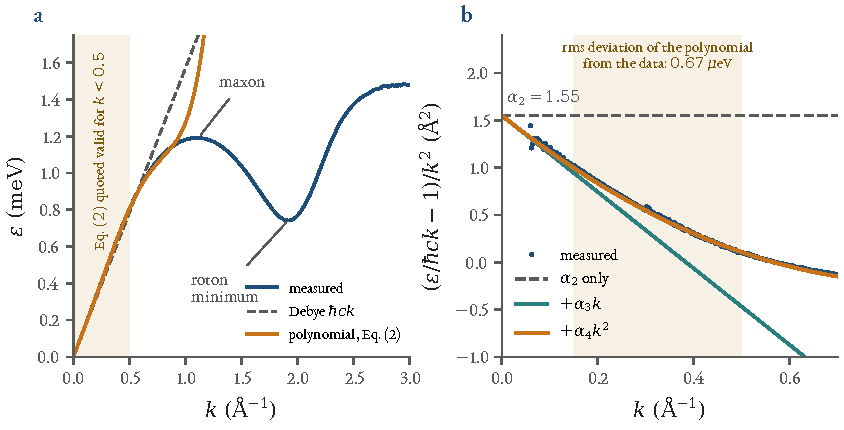
\includegraphics[width=\linewidth]{figures/ch04_dispersion.pdf}
\caption[The phonon branch of superfluid helium-4 measured by neutron scattering]{The phonon branch of superfluid $^4$He at saturated vapour pressure ($T<0.1\cfK$), measured by neutron scattering (ancillary data of \cite{Godfrin2021}, CC BY 4.0). \textbf{(a)} The measured curve (blue), the linear Debye dispersion (dashed grey) and the polynomial of Eq.~(2) of the paper with the coefficient set quoted there (orange); maxon at $k=\cfv{maxon-k}\ \cfAng^{-1}$, roton minimum at $k=\cfv{roton-k}\ \cfAng^{-1}$, $\varepsilon/\cfkB=\cfv{roton-K}\cfK$ in this table. \textbf{(b)} The same data divided by $\hbar ck$ and $k^2$: the intercept is $\alpha_2$, the slope $\alpha_3$, the curvature $\alpha_4$. The rms difference between the polynomial and the table for $0.15\le k\le0.5\ \cfAng^{-1}$ is $\cfv{rms-ueV}\ \mu$eV.}\label{ch04:fig-dispersion}
\end{figure}

Real helium is not linear.
The paper writes the phonon branch as a power series
\begin{equation}\label{ch04:eq-disp}
 \varepsilon(k)=\hbar c\,k\,\bigl(1+\alpha_2k^2+\alpha_3k^3+\alpha_4k^4+\alpha_5k^5+\alpha_6k^6\bigr),
\end{equation}
with no linear term in the bracket ($\alpha_1=0$); $\alpha_j$ has the dimension of length$^j$.
For saturated vapour pressure it quotes $c=\cfv{c}\ \mathrm{m\,s^{-1}}$, $\alpha_2=\cfv{a2}\ \cfAng^2$, $\alpha_3=\cfv{a3}\ \cfAng^3$, $\alpha_4=\cfv{a4}\ \cfAng^4$ and $\alpha_5=\alpha_6=0$, and says that this set describes the measured dispersion for $k<0.5\ \cfAng^{-1}$.
\Cref{ch04:fig-dispersion} compares it with the open table: within the shaded range the polynomial and the data differ by $\cfv{rms-ueV}\ \mu$eV rms and by at most $\cfv{maxdev-ueV}\ \mu$eV, and at $k=1\ \cfAng^{-1}$ the polynomial lies $\cfv{poly-dev-1}$ per cent above the data: beyond its range it stops describing helium and becomes a sequence of numbers (that is not a criticism, the range is quoted with the coefficients; it is the first hint of what a series in $T$ can and cannot do).

The sign of $\alpha_2$ matters physically.
For $\alpha_2>0$ the energy at a given $k$ lies above the linear Debye value, so there are fewer thermal phonons than in a Debye gas and $C_V/T^3$ \emph{falls} as the temperature rises: this is the slow drift of the first paragraph.
(The same sign, the ``anomalous'' dispersion, keeps the collinear decay of a phonon into two phonons energetically open: this is \Lthm{HeliumKinematics}{three_phonon_open_iff}, for a dispersion $ck(1+ak^2)$; \cref{ch05} treats it.)

\subsection{A series in \texorpdfstring{$T$}{T}}
To turn \eqref{ch04:eq-energy} into a series one needs the integral over energy, not over wavevector.
Write $u=\varepsilon/\hbar c$, which has the dimension of an inverse length, so that $u=k(1+\alpha_2k^2+\dots)$, and invert the series:
\begin{equation}\label{ch04:eq-inverse}
 k(u)=u-\alpha_2u^3-\alpha_3u^4+(3\alpha_2^2-\alpha_4)u^5+(7\alpha_2\alpha_3-\alpha_5)u^6+\eta\,u^7+O(u^8),
\end{equation}
with $\eta=-12\alpha_2^3+8\alpha_2\alpha_4+4\alpha_3^2-\alpha_6$.
This is the inverse series printed in the paper, here for $\alpha_1=0$ (the paper prints it for general $\alpha_1$).
The density of states in $u$ is $k^2\,\mathrm dk/\mathrm du=\sum_n g_n u^n$ with
\begin{equation}\label{ch04:eq-dos}
\begin{aligned}
 g_2&=1,\quad g_3=0,\quad g_4=-5\alpha_2,\quad g_5=-6\alpha_3,\quad g_6=7(4\alpha_2^2-\alpha_4),\\
 g_7&=8(9\alpha_2\alpha_3-\alpha_5),\quad g_8=-3(55\alpha_2^3-30\alpha_2\alpha_4-15\alpha_3^2+3\alpha_6).
\end{aligned}
\end{equation}
Each monomial $g_nu^n$ gives a thermal integral that is a Bose integral,
\begin{equation}\label{ch04:eq-bose}
 \int_0^\infty\frac{u^{m}}{e^{\hbar cu/\cfkB T}-1}\,\mathrm du=\Bigl(\frac{\cfkB T}{\hbar c}\Bigr)^{m+1}\,m!\,\zeta(m+1),
\end{equation}
so that
\begin{align}
 E(T)&=\frac{V}{2\pi^2}\sum_n g_n\,(n+1)!\,\zeta(n+2)\,\frac{(\cfkB T)^{n+2}}{(\hbar c)^{n+1}},\label{ch04:eq-series-E}\\
 C_V&=\sum_n\frac{V\cfkB^{\,n+2}}{2\pi^2(\hbar c)^{n+1}}\,g_n\,(n+2)!\,\zeta(n+2)\;T^{\,n+1}.\label{ch04:eq-series}
\end{align}
The term $n=2$ is Debye's.
The term $n=3$ would give a $T^4$ term, but $g_3=0$ because there is no $\alpha_1$: that is why Eq.~(22) has no $B\,T^4$.
The terms $n=4,5,6,7,8$ give $C\,T^5$, $D\,T^6$, $E\,T^7$, $K\,T^8$, $L\,T^9$, and the result is \cref{ch04:tab-coeffs}.

\begin{table}[t]\centering\small
\caption{The six coefficients of Eq.~(22). Column $g_n$: bracket of the density of states \eqref{ch04:eq-dos}; column $I_n$: the Bose integral $\int_0^\infty t^{n+1}/(e^t-1)\,\mathrm dt=(n+1)!\,\zeta(n+2)$ (all six values are proved in Lean, Section~\ref{ch04:sec-lean}); last two columns: the closed form evaluated with the coefficient set of the paper (units $\mathrm{J\,mol^{-1}K^{-p}}$, $p$ the power of $T$; values from \texttt{figures/ch04\_common.py}), and the number printed in the paper.}\label{ch04:tab-coeffs}
\renewcommand{\arraystretch}{1.25}
\begin{tabular}{@{}llllrr@{}}\toprule
 & $T^p$ & $g_n$ & $I_n$ & computed & printed \\ \midrule
 $A$ & $T^3$ & $1$ & $\pi^4/15$ & \cfv{A-val} & \cfv{A-pr} \\
 $C$ & $T^5$ & $-5\alpha_2$ & $8\pi^6/63$ & \cfv{C-val} & \cfv{C-pr} \\
 $D$ & $T^6$ & $-6\alpha_3$ & $720\,\zeta(7)$ & \cfv{D-val} & \cfv{D-pr} \\
 $E$ & $T^7$ & $7(4\alpha_2^2-\alpha_4)$ & $8\pi^8/15$ & \cfv{E-val} & \cfv{E-pr} \\
 $K$ & $T^8$ & $8(9\alpha_2\alpha_3-\alpha_5)$ & $40320\,\zeta(9)$ & \cfv{K-val} & \cfv{K-pr} \\
 $L$ & $T^9$ & $-3(55\alpha_2^3-30\alpha_2\alpha_4-15\alpha_3^2+3\alpha_6)$ & $128\pi^{10}/33$ & \cfv{L-val} & \cfv{L-pr} \\ \bottomrule
\end{tabular}
\end{table}

Written out, with $\zeta$ the Riemann zeta function, the six coefficients are
\begin{align*}
 A&=\frac{2\pi^2\cfkB^4V}{15\,c^3\hbar^3}, &
 C&=-\frac{40\,\pi^4\alpha_2\cfkB^6V}{21\,c^5\hbar^5},\\
 D&=-\frac{15120\,\alpha_3\cfkB^7V\,\zeta(7)}{\pi^2c^6\hbar^6}, &
 E&=\frac{224\,\pi^6\cfkB^8V\,(4\alpha_2^2-\alpha_4)}{15\,c^7\hbar^7},\\
 K&=\frac{1451520\,\cfkB^9V\,\zeta(9)\,(9\alpha_2\alpha_3-\alpha_5)}{\pi^2c^8\hbar^8},\\
 L&=-\frac{640\,\pi^8\cfkB^{10}V\,(55\alpha_2^3-30\alpha_2\alpha_4-15\alpha_3^2+3\alpha_6)}{11\,c^9\hbar^9}.
\end{align*}
Three features are structural, not matters of presentation.
First, $\pi$ appears in $A,C,E,L$ and $\zeta(7)$, $\zeta(9)$ in $D$ and $K$: even zeta values at $2k$ are rational multiples of $\pi^{2k}$ (Bernoulli numbers), odd ones are not known in closed form, and \eqref{ch04:eq-series} contains $\zeta(n+2)$, which is even for $n$ even and odd for $n$ odd.
Second, the coefficients are not one-to-one with the $\alpha_j$: $E$ contains $\alpha_2$ and $\alpha_4$, $L$ contains $\alpha_2$, $\alpha_3$, $\alpha_4$ and $\alpha_6$, so a measurement of $E$ gives a combination of dispersion coefficients, not $\alpha_4$.
Third, the printed numbers of \cref{ch04:tab-coeffs} follow from the printed formulas at the quoted coefficients to within $\cfv{coef-maxdiff}$ per cent (the quoted $\alpha_j$ are themselves rounded, so a few parts in $10^3$ carry no information).
That is a check of the paper's arithmetic; it is not yet a check of its formulas, which is where an error of an earlier series would have lived.


%% ====================================================================================================================
\section{What the proof assistant says}\label{ch04:sec-lean}

The library \texttt{QuantumFluids} has three modules for this chapter, \texttt{BoseIntegral}, \texttt{PhononSeries} and \texttt{PhononSpecificHeat}, with a design note recording how the work was done (the file \texttt{PHONON\_SERIES\_A\_TO\_L.md} in the \texttt{docs/designs} directory of the repository).
\Cref{ch02} explains how to read Lean; here it is enough to know that a \texttt{theorem} is a statement together with a proof that the kernel has checked, and that the statements below are copied from the library unchanged.
For this book the three modules were compiled, in dependency order, with Lean \cfv{lean-toolchain} against the library's Mathlib: no errors, no \texttt{sorry}.
The only axioms used are the three of classical mathematics (\texttt{propext}, \texttt{Classical.choice}, \texttt{Quot.sound}) for \texttt{BoseIntegral} and \texttt{PhononSpecificHeat}, and just \texttt{propext} and \texttt{Quot.sound} for \texttt{PhononSeries}, which is pure ring theory.

\subsection{Step one: the Bose integral}
Every coefficient of Eq.~(22) rests on one identity, $\int_0^\infty t^n/(e^t-1)\,\mathrm dt=n!\,\zeta(n+1)$.
Mathlib has the Gamma integral and $\zeta(2k)$ in closed form, but not this integral, so the library proves it.

\begin{leanbox}{BoseIntegral}
\begin{lstlisting}[style=lean,basicstyle=\ttfamily\footnotesize]
/-- The Bose factor `1/(eᵗ − 1)`, complex-valued so that Mathlib's `mellin` applies. -/
noncomputable def bose (t : ℝ) : ℂ := ((1 / (rexp t - 1) : ℝ) : ℂ)

theorem bose_integral_nat {n : ℕ} (hn : 1 ≤ n) :
    mellin bose (n + 1) = (Nat.factorial n : ℂ) * riemannZeta (n + 1)
-- statement only; the proof is in lean_src/BoseIntegral.lean
\end{lstlisting}
\end{leanbox}

\noindent In words.
Mathlib's \lean{mellin f s} is by definition $\int_0^\infty t^{s-1}f(t)\,\mathrm dt$, so \lean{mellin bose (n + 1)} \emph{is} the integral $\int_0^\infty t^n/(e^t-1)\,\mathrm dt$.
The first theorem, \Lthm{BoseIntegral}{bose_integral_nat}, says it equals $n!\,\zeta(n+1)$ for every $n\ge1$: this is \eqref{ch04:eq-bose} with the temperature scaled out.
A companion theorem, \Lthm{BoseIntegral}{debye_specific_heat}, says that the energy $\pi^2V(\cfkB T)^4/30(\hbar c)^3$ of the Debye gas, whose integral is the case $n=3$ (\Lthm{BoseIntegral}{mellin_bose_four}: \lean{mellin bose 4} $=\pi^4/15$), has the derivative $A\,T^3$ with $A=2\pi^2\cfkB^4V/15c^3\hbar^3$, the coefficient printed in the paper.
\emph{Proof idea (abridged).} For $t>0$ one has $1/(e^t-1)=\sum_{m\ge0}e^{-(m+1)t}$, the geometric series behind Bose statistics (\Lthm{BoseIntegral}{hasSum_bose}); Mathlib's \lean{hasSum\_mellin} integrates a series of exponentials term by term, each term giving $\Gamma(s)/(m+1)^s$; the sum is $\Gamma(s)\zeta(s)$, and $\Gamma(n+1)=n!$.

\subsection{Step two: inverting the dispersion and counting states, without analysis}
The next module is where the printed series meet algebra.
The claim ``$k(u)$ is the inverse series up to $O(u^8)$'' involves a truncation, and a truncation normally brings questions of convergence with it.
The library avoids them.
\emph{Equal up to $O(e^8)$} is stated as an identity in an arbitrary commutative ring $R$ with an element $e$ such that $e^8=0$.
Taking $R$ to be the ring of power series modulo $e^8$ recovers the usual statement; nothing about limits is needed, and the theorem is pure ring theory.

\begin{leanbox}{PhononSeries}
\begin{lstlisting}[style=lean,basicstyle=\ttfamily\footnotesize]
variable {R : Type*} [CommRing R]

/-- The inverse series for `alpha_1 = 0`, the case the paper's Eq. (22) treats. -/
def kInv0 (a2 a3 a4 a5 a6 e : R) : R :=
  -12*a2^3*e^7 + 3*a2^2*e^5 + 7*a2*a3*e^6 + 8*a2*a4*e^7 - a2*e^3 + 4*a3^2*e^7 - a3*e^4 - a4*e^5 - a5*e^6 - a6*e^7 + e

/-- Its formal derivative with respect to `e`. -/
def kInv0Deriv (a2 a3 a4 a5 a6 e : R) : R :=
  -84*a2^3*e^6 + 15*a2^2*e^4 + 42*a2*a3*e^5 + 56*a2*a4*e^6 - 3*a2*e^2 + 28*a3^2*e^6 - 4*a3*e^3 - 5*a4*e^4 - 6*a5*e^5 - 7*a6*e^6 + 1

theorem density_of_states (a2 a3 a4 a5 a6 e : R) (h : e ^ 9 = 0) :
    kInv0 a2 a3 a4 a5 a6 e ^ 2 * kInv0Deriv a2 a3 a4 a5 a6 e
      = e ^ 2 - 5 * a2 * e ^ 4 - 6 * a3 * e ^ 5 + 7 * (4 * a2 ^ 2 - a4) * e ^ 6
        + 8 * (9 * a2 * a3 - a5) * e ^ 7
        - 3 * (55 * a2 ^ 3 - 30 * a2 * a4 - 15 * a3 ^ 2 + 3 * a6) * e ^ 8
-- statement only; the proof is in lean_src/PhononSeries.lean
\end{lstlisting}
\end{leanbox}

\noindent In words.
The module proves two theorems.
The first, \Lthm{PhononSeries}{dispersion_kInv}, says that the inverse series printed in the paper, for general $\alpha_1$ and through $(\omega/c)^7$ with the coefficient $\eta$, really inverts $u=k(1+\alpha_1k+\dots+\alpha_6k^6)$: substitute it in and you get $e$ back, modulo $e^8$ (it is stated for the series \lean{kInv} of general $\alpha_1$, of which \lean{kInv0} is the case $\alpha_1=0$).
The second, shown above, \Lthm{PhononSeries}{density_of_states}, says that $k^2\,\mathrm dk/\mathrm du$, computed from the series \eqref{ch04:eq-inverse} for $\alpha_1=0$ and its derivative, equals the polynomial whose coefficients are the brackets \eqref{ch04:eq-dos}, modulo $e^9$.
The missing term $e^3$ is the missing $B\,T^4$.
\emph{Proof idea (abridged).} The powers $k^2,\dots,k^7$ of the series are truncated one at a time, each step a statement of the form \lean{linear\_combination (r) * h} with $h:\ e^8=0$.
This tactic asks the kernel to check that (left side $-$ right side) $-\,r\cdot e^N$ vanishes identically as a polynomial ($N=8$ or $9$); $r$ is the \emph{certificate}.
Here is the shape of one such proof, with its certificate shortened:
\begin{lstlisting}[style=lean,basicstyle=\ttfamily\footnotesize]
theorem kSq0_eq (a2 a3 a4 a5 a6 e : R) (h : e ^ 9 = 0) :
    kInv0 a2 a3 a4 a5 a6 e ^ 2 = kSq0 a2 a3 a4 a5 a6 e := by
  unfold kInv0 kSq0
  linear_combination (144*a2^6*e^5 - 72*a2^5*e^3 - 168*a2^4*a3*e^4 - 192*a2^4*a4*e^5 + ...) * h
\end{lstlisting}
\noindent (proof abridged: the certificate has \cfv{cert-kSq0} terms; the six certificates for the powers $k^2,\dots,k^7$ of the general inverse series have \cfv{cert-list} terms.)
The certificates were produced by a computer-algebra script and are \emph{checked, not trusted}: had the script made an error the kernel would reject the proof.
The design note records this module as the first generated proof file in the library.

\subsection{Step three: the six coefficients}
The last module assembles the two ingredients.
The energy carried by the monomial $g\,u^n$ of the density of states is, from \eqref{ch04:eq-series-E}, $\frac{V}{2\pi^2}\,g\,I\,\cfkB^{n+2}T^{n+2}/(\hbar c)^{n+1}$ with $I=\int_0^\infty t^{n+1}/(e^t-1)\,\mathrm dt$ the Bose integral.
The library calls it \Lthm{PhononSpecificHeat}{energyTerm}.

\begin{leanbox}{PhononSpecificHeat}
\begin{lstlisting}[style=lean,basicstyle=\ttfamily\footnotesize]
noncomputable def energyTerm (V kB hbar c g : ℝ) (n : ℕ) (I T : ℝ) : ℝ :=
  V / (2 * π ^ 2) * g * I * kB ^ (n + 2) / (hbar * c) ^ (n + 1) * T ^ (n + 2)

theorem phonon_specific_heat (V kB hbar c a2 a3 a4 a5 a6 z7 z9 T : ℝ) (hh : hbar ≠ 0) (hc : c ≠ 0) :
    HasDerivAt (fun T =>
        energyTerm V kB hbar c 1 2 (π ^ 4 / 15) T
      + energyTerm V kB hbar c (-5 * a2) 4 (8 * π ^ 6 / 63) T
      + energyTerm V kB hbar c (-6 * a3) 5 (720 * z7) T
      + energyTerm V kB hbar c (7 * (4 * a2 ^ 2 - a4)) 6 (8 * π ^ 8 / 15) T
      + energyTerm V kB hbar c (8 * (9 * a2 * a3 - a5)) 7 (40320 * z9) T
      + energyTerm V kB hbar c (-3 * (55 * a2 ^ 3 - 30 * a2 * a4 - 15 * a3 ^ 2 + 3 * a6)) 8
          (128 * π ^ 10 / 33) T)
      ( 2 * π ^ 2 * kB ^ 4 * V / (15 * c ^ 3 * hbar ^ 3) * T ^ 3
      + -(40 * (π ^ 4 * a2 * kB ^ 6 * V)) / (21 * (c ^ 5 * hbar ^ 5)) * T ^ 5
      + -(15120 * (a3 * kB ^ 7 * V * z7)) / (π ^ 2 * c ^ 6 * hbar ^ 6) * T ^ 6
      + 224 * π ^ 6 * kB ^ 8 * V * (4 * a2 ^ 2 - a4) / (15 * c ^ 7 * hbar ^ 7) * T ^ 7
      + 1451520 * kB ^ 9 * V * z9 * (9 * a2 * a3 - a5) / (π ^ 2 * c ^ 8 * hbar ^ 8) * T ^ 8
      + -(640 * (π ^ 8 * kB ^ 10 * V * (55 * a2 ^ 3 - 30 * a2 * a4 - 15 * a3 ^ 2 + 3 * a6)))
          / (11 * (c ^ 9 * hbar ^ 9)) * T ^ 9) T
-- statement only; the proof is in lean_src/PhononSpecificHeat.lean
\end{lstlisting}
\end{leanbox}

\noindent In words.
A theorem proved earlier in the module, \Lthm{PhononSpecificHeat}{bose_integral_values}, gives the six Bose integrals of \cref{ch04:tab-coeffs} in closed form: $\int_0^\infty t^3/(e^t-1)\,\mathrm dt=\pi^4/15$, then $8\pi^6/63$, $720\,\zeta(7)$, $8\pi^8/15$, $40320\,\zeta(9)$, $128\pi^{10}/33$ (as \lean{mellin bose 4}, $\dots$, \lean{mellin bose 10}).
The even ones use Mathlib's $\zeta(2k)$ through Bernoulli numbers (the library computes $B_6=\tfrac1{42}$, $B_8=-\tfrac1{30}$, $B_{10}=\tfrac5{66}$, because Mathlib's table stops at $B_4$, and from them $\zeta(6)=\pi^6/945$, $\zeta(8)=\pi^8/9450$, $\zeta(10)=\pi^{10}/93555$); the odd ones stay symbolic.
The capstone \Lthm{PhononSpecificHeat}{phonon_specific_heat} says: \emph{the derivative with respect to $T$ of the sum of the six energy terms --- with the density-of-states brackets of \lean{density\_of\_states} and the six Bose integrals --- is exactly the six printed closed forms $A,C,D,E,K,L$}.
The two odd zeta values enter as real parameters \lean{z7}, \lean{z9}; \lean{bose\_integral\_values} is where they are tied to \lean{riemannZeta 7} and \lean{riemannZeta 9}, which keeps the capstone in $\mathbb R$ and makes the absence of a closed form visible in the type.
\emph{Proof idea (abridged).} Each term differentiates by the power rule; \lean{HasDerivAt.add} is applied five times; the two sides then differ only by rearrangement, which \lean{field\_simp} and \lean{ring} close.

\subsection{Closing the links that were made by inspection}\label{ch04:sec-newlean}
Reading the three boxes again, one sees what the design note itself records as the weak points: the chain from the dispersion to Eq.~(22) is assembled by \emph{retyping}.
The brackets $1,-5\alpha_2,-6\alpha_3,\dots$ in the capstone were copied from \lean{density\_of\_states}; no theorem says that they are the coefficients of the polynomial \lean{kInv0}$^2\cdot$\lean{kInv0Deriv}.
\lean{kInv0Deriv} was typed in, not computed as a derivative.
And the six values of $I$ in the capstone were retyped from \lean{bose\_integral\_values}.
None of these is likely to hide an error, but it is exactly the kind of gap that a ``machine-checked'' label can paper over.


The file \texttt{lean/Ch04\_DosLink.lean} of this book removes the retypings.
It is \emph{new Lean, written for this book and not part of the library}: it imports the three modules above, lives in the namespace \texttt{QuantumFluids.DosLink}, and compiles in about a minute against the same Mathlib, with no error and no \lean{sorry}; its \lean{\#print axioms} lines show the three axioms of classical mathematics and nothing else.

\begin{leanbox}{new: Ch04\_DosLink}
\begin{lstlisting}[style=lean,basicstyle=\ttfamily\footnotesize]
/-- The inverse series with the dispersion coefficients as constant polynomials, evaluated at `X`. -/
noncomputable def kPoly (a2 a3 a4 a5 a6 : ℝ) : ℝ[X] :=
  kInv0 (C a2) (C a3) (C a4) (C a5) (C a6) X

theorem derivative_kPoly (a2 a3 a4 a5 a6 : ℝ) :
    derivative (kPoly a2 a3 a4 a5 a6) = kInv0Deriv (C a2) (C a3) (C a4) (C a5) (C a6) X

/-- The density-of-states polynomial `k(e)^2 * dk/de`, with `dk/de` the formal derivative. -/
noncomputable def dosPoly (a2 a3 a4 a5 a6 : ℝ) : ℝ[X] :=
  kPoly a2 a3 a4 a5 a6 ^ 2 * derivative (kPoly a2 a3 a4 a5 a6)

theorem dos_coeffs (a2 a3 a4 a5 a6 : ℝ) :
    (dosPoly a2 a3 a4 a5 a6).coeff 2 = 1 ∧
    (dosPoly a2 a3 a4 a5 a6).coeff 3 = 0 ∧
    (dosPoly a2 a3 a4 a5 a6).coeff 4 = -5 * a2 ∧
    (dosPoly a2 a3 a4 a5 a6).coeff 5 = -6 * a3 ∧
    (dosPoly a2 a3 a4 a5 a6).coeff 6 = 7 * (4 * a2 ^ 2 - a4) ∧
    (dosPoly a2 a3 a4 a5 a6).coeff 7 = 8 * (9 * a2 * a3 - a5) ∧
    (dosPoly a2 a3 a4 a5 a6).coeff 8 = -3 * (55 * a2 ^ 3 - 30 * a2 * a4 - 15 * a3 ^ 2 + 3 * a6)
\end{lstlisting}
\begin{lstlisting}[style=lean,basicstyle=\ttfamily\fontsize{7.2}{8.6}\selectfont]
theorem phonon_specific_heat_end_to_end (V kB hbar c a2 a3 a4 a5 a6 T : ℝ) (hh : hbar ≠ 0) (hc0 : c ≠ 0) :
    HasDerivAt (fun T =>
        energyTerm V kB hbar c ((dosPoly a2 a3 a4 a5 a6).coeff 2) 2 (mellin bose 4).re T
      + energyTerm V kB hbar c ((dosPoly a2 a3 a4 a5 a6).coeff 4) 4 (mellin bose 6).re T
      + energyTerm V kB hbar c ((dosPoly a2 a3 a4 a5 a6).coeff 5) 5 (mellin bose 7).re T
      + energyTerm V kB hbar c ((dosPoly a2 a3 a4 a5 a6).coeff 6) 6 (mellin bose 8).re T
      + energyTerm V kB hbar c ((dosPoly a2 a3 a4 a5 a6).coeff 7) 7 (mellin bose 9).re T
      + energyTerm V kB hbar c ((dosPoly a2 a3 a4 a5 a6).coeff 8) 8 (mellin bose 10).re T)
      (…) T      -- abridged: the six closed forms of `phonon_specific_heat`, not repeated
-- statements only; the proofs are in lean/Ch04_DosLink.lean
\end{lstlisting}
\end{leanbox}

\noindent In words.
\Lthm{DosLink}{kPoly} is the inverse series \lean{kInv0} with the dispersion coefficients as constant polynomials, evaluated at the variable $X$ of $\mathbb R[X]$; \Lthm{DosLink}{derivative_kPoly} says that Mathlib's formal derivative of it \emph{is} \lean{kInv0Deriv}, which is thus no longer typed in.
\Lthm{DosLink}{dosPoly} is $k^2\cdot k'$ as an honest polynomial, and \Lthm{DosLink}{dos_coeffs} says that its coefficients in degrees $2$ to $8$ are exactly the brackets \eqref{ch04:eq-dos}, the absent degree~$3$ included.
\Lthm{DosLink}{phonon_specific_heat_end_to_end} is Eq.~(22) with nothing retyped: the brackets are read off \lean{dosPoly}, the six Bose integrals are the real parts of \lean{mellin bose 4}, \dots, \lean{mellin bose 10}, and the two odd zeta values are $\zeta(7)$ and $\zeta(9)$ themselves.

\emph{Proof idea (abridged).} Apply \Lthm{PhononSeries}{density_of_states} not in $\mathbb R$ but in the ring $\mathbb R[X]/(X^9)$, where $e=X$ satisfies $e^9=0$.
It says that $k^2k'$ and the polynomial of brackets are equal there, that is, that $X^9$ divides their difference, and a polynomial divisible by $X^9$ has vanishing coefficients below degree $9$ (\lean{Polynomial.X\_pow\_dvd\_iff}).
The end-to-end theorem then follows from \Lthm{PhononSpecificHeat}{phonon_specific_heat} and \Lthm{PhononSpecificHeat}{bose_integral_values}.

The file goes one step further.
It defines the energy of the monomial $g\,u^n$ as the integral itself, written with Mathlib's Mellin transform (\lean{energyMonomial}); proves, in \Lthm{DosLink}{energyMonomial_eq}, that for $T>0$ it equals \lean{energyTerm} evaluated with the Bose integral $\operatorname{Re}\,\lean{mellin bose (n + 2)}$; and restates Eq.~(22), in \Lthm{DosLink}{phonon_specific_heat_integral}, for the sum of the six integrals.


\paragraph{What is still outside Lean.}
What these theorems say is exact and limited: the derivative of the thermal energy of the \emph{truncated} density of states $\sum_{n=2}^{8}g_nu^n$, integrated against the Bose factor over $(0,\infty)$, is Eq.~(22).
That the truncated sum may stand for the true density of states under the integral --- that the series is an asymptotic expansion of the specific heat of a given dispersion curve, with the roton branch and the upper limit dropped --- is an analytical statement that the library does not contain.
Section~\ref{ch04:sec-data} computes what it amounts to.



%% ====================================================================================================================
\section{A confirmation, not a finding}\label{ch04:sec-confirm}

Lean is one derivation.
Two others were made without it, for the reason that two thermometers matter: a proof assistant checks a \emph{statement}, so it can confirm a derivation that started from the wrong statement just as faithfully as from the right one.

\paragraph{A symbolic derivation.}
The script \texttt{exploration/godfrin/derive\_cv\_series.py} derives everything from scratch with the computer-algebra system sympy: it reverts the series order by order, forms $\mathrm d(k^3/3)/\mathrm du$, integrates term by term with the Bose integral \eqref{ch04:eq-bose}, differentiates, and compares each result with the printed closed form by the exact test \lean{simplify(derived - printed) == 0}, which leaves no room for tuning.
I re-ran it for this book (\cfv{sympy-seconds} s on the shared machine); its output ends:
\begin{lstlisting}[style=plainmono,basicstyle=\ttfamily\footnotesize]
A (T^3): MATCHES the printed closed form      C (T^5): MATCHES the printed closed form
D (T^6): MATCHES the printed closed form      E (T^7): MATCHES the printed closed form
K (T^8): MATCHES the printed closed form      L (T^9): MATCHES the printed closed form
T^4 coefficient (paper: absent because alpha_1 = 0): 0
INVERSE SERIES: all 7 printed coefficients match
C_V SERIES: ALL SIX MATCH
\end{lstlisting}
(``All 7'' counts the seven coefficients of the printed inverse series for general $\alpha_1$, through $(\omega/c)^7$.)

\paragraph{Exact rational arithmetic.}
The third derivation is this chapter's own, written to be as unlike the other two as possible: no symbols, no proof, only fractions.
With the coefficient set of the paper as the exact fractions $\alpha_2=31/20$, $\alpha_3=-101/25$, $\alpha_4=23/10$, the script \texttt{figures/ch04\_series\_ext.py} reverts the series by fixed-point iteration in Python's \texttt{fractions} and reads off the density-of-states coefficients, $g_4=-31/4$, $g_5=606/25$, $g_6=5117/100$, $g_7=-56358/125$, $g_8=3527061/8000$: the brackets \eqref{ch04:eq-dos} at those $\alpha$'s, obtained by a program that has never seen them.
Multiplying by the Bose integrals gives the coefficient of each power of $T$; the six that Eq.~(22) predicts agree with the closed forms to a relative \cfv{rat-maxdiff} (double-precision rounding), and the coefficient of $T^4$ is exactly zero.
The same script continues past $L$, giving $c_{10}=\cfv{c10}$ and $c_{11}=\cfv{c11}$ (in $\mathrm{J\,mol^{-1}K^{-p}}$): Lean does not cover those, the exact arithmetic does, and Section~\ref{ch04:sec-data} uses them.

\paragraph{What kind of check this is.}
An earlier pass in the programme had only reproduced the six printed \emph{numbers} from the six printed \emph{formulas} (the last column of \cref{ch04:tab-coeffs}).
That tests the arithmetic of the paper, not its formulas, and a formula is where an error of an earlier series would live.
The programme's rule LL-15 (name the property a claim depends on, and check that property rather than a neighbour of it) asks for a derivation from the dispersion relation, and that is what the three above are.
They agree with Eq.~(22) in all six coefficients, with the inverse series, and with the absence of a $T^4$ term.

\paragraph{Checkers must be able to fail.}
A proof checker that cannot reject anything proves nothing.
When the Lean proofs were first written, four deliberately wrong versions were fed to it --- $-12\alpha_2^3$ in $\eta$ changed to $-11\alpha_2^3$, the $15120$ of $D$ to $15121$, the $9\alpha_2\alpha_3$ of $K$ to $8\alpha_2\alpha_3$, the $55$ of $L$ to $54$ --- and all four were rejected (design note).
I repeated two of them for this book, against the library modules compiled as above (the files \texttt{lean/Ch04\_NegativeControl\_L54.lean} and \texttt{lean/Ch04\_NegativeControl\_D15121.lean} are meant to fail; paths shortened in what follows, and the dagger that Lean prints after inaccessible names removed).
Changing $55$ to $54$ in \Lthm{PhononSeries}{density_of_states}, with the certificate of the true theorem, gives:
\lstinputlisting[style=plainmono,basicstyle=\ttfamily\footnotesize]{figures/ch04_negctl_L54.txt}
\noindent and changing the $15120$ of $D$ to $15121$ in the capstone \Lthm{PhononSpecificHeat}{phonon_specific_heat} gives:
\lstinputlisting[style=plainmono,basicstyle=\ttfamily\footnotesize]{figures/ch04_negctl_D15121.txt}
\noindent In the first case \lean{ring} prints the residue: the two sides differ by $-3a_2^3e^8$, exactly what changing $55$ to $54$ in the term $-3(55a_2^3-\dots)e^8$ must leave behind.
In the second the message is a polynomial identity that \lean{ring} could not close, too long to show; what matters is that it was not closed.
A proof that fails, with a residue one can read, is a checker doing its work.

\paragraph{The outcome rule, and a lapse.}
The programme's discipline is to fix, before running a check, what each outcome will be called.
Here that was \emph{not} done: the derivation script was written and run first and the rule below afterwards, and the design note records a process lapse.
Because the comparison is a symbolic identity, with no tolerance to tune and no analysis choice (the coefficients to compare are the paper's own), the lapse cannot have shaped the result; it is recorded all the same.
The rule that binds what follows: a mismatch would have been a candidate misprint of the preprint, to be settled against the published version before anything is said about the paper; a full match is a confirmation, and \emph{is not to be dressed up as a finding}.
It was a full match, for the arXiv version; the version of record was not compared.
Eq.~(22) is a correct consequence of Eq.~(2), as a statement of mathematics.
That is a good thing to know about a series whose predecessors were wrong, and it is all it is.


%% ====================================================================================================================
\section{What the solver says}\label{ch04:sec-solver}

The solver is a witness for a different question.
Lean says that, for the polynomial dispersion \eqref{ch04:eq-disp}, the coefficients of the series in $T$ are what Eq.~(22) says.
A solver that has never heard of a series can be asked whether the \emph{integral itself} behaves as that series says.
Two experiments follow.
Neither is a proof: each carries a tolerance below which it is blind, and each concerns the model polynomial and not helium.
All integrals use CVODE of rusty-SUNDIALS through its Python module (\texttt{rusty\_sundials.CvodeSolver}), with the Adams--Moulton option, the natural one for smooth non-stiff problems.

\paragraph{Which build of the solver.}
My first runs used the module installed in the project's virtual environment (built 2026-09-26) and gave plausible numbers that were wrong: at relative tolerance $10^{-6}$ its Adams method returned the Debye integral $\int_0^{70}x^3/(e^x-1)\,\mathrm dx$ with a relative error $\cfv{old-adams-bose-err}$ after $\cfv{old-adams-bose-calls}$ right-hand-side calls, $\cfv{old-adams-bose-ratio}$ times the tolerance, and its BDF gave up (``too many error test failures at one step'') on \cfv{old-bdf-landing-err} of \cfv{probe-landing-n} end points when asked for the six Bose integrals of the next subsection (\texttt{figures/ch04\_solver\_probe.py}).
The maintainers' note \texttt{docs/CVODE\_ADAMS\_FIX.md} in the rusty-SUNDIALS repository describes the cause: in that build \lean{Method::Adams} was implicit Euler with a Milne error estimate, a first-order method whose error scales like $\sqrt{\mathrm{rtol}}$, as observed; it was fixed on 2026-09-28.
Every number of this chapter comes from a build of rusty-SUNDIALS commit \cfv{rs-commit-short} (sha256 of \texttt{rusty\_sundials.so} beginning \cfv{rs-sha-short}), and the scripts refuse to run with any other: Adams on $y'=-y$ over $[0,10]$ at relative tolerance $10^{-8}$ must use fewer than $5000$ right-hand-side calls (it uses \cfv{new-adams-decay-calls}).
With that build the Debye integral costs $\cfv{new-adams-bose-calls}$ calls at relative tolerance $10^{-6}$ and returns a relative error $\cfv{new-adams-bose-err}$, and no end point defeats Adams or BDF (\cfv{new-landing-err} give-ups).
A numerical result with the right shape is not evidence that the tool is right; a check against a closed form is.

\subsection{The Bose integrals as initial-value problems}
The integral $\int_0^X t^m/(e^t-1)\,\mathrm dt$ is the value at $x=X$ of the solution of $y'=x^m/(e^x-1)$, $y(0)=0$.
Scaling by $m!$ makes all six components of order one ($y_m\to\zeta(m+1)$), which lets one scalar absolute tolerance serve all of them.
The comparison is with the closed forms \emph{proved in Lean} (\cref{ch04:tab-coeffs}), not with a numerically evaluated $m!\,\zeta(m+1)$.

\begin{rustbox}{CVODE: the six Bose integrals}
\begin{lstlisting}[style=py,basicstyle=\ttfamily\footnotesize]
def rhs_bose(x, y):                    # y_m' = x^m / (m! (e^x - 1)),  y_m(0) = 0
    if x <= 0.0:
        return [0.0]*len(ms)
    e = np.expm1(x)
    return [x**m/(fact[m]*e) for m in ms]
# ms = [3, 5, 6, 7, 8, 9];  excerpt of figures/ch04_cvode_compute.py
solver = rs.CvodeSolver("adams", rtol, atol, 200_000)    # method, rtol, atol, max_steps
_, y = solver.solve(rhs_bose, 0.0, [0.0]*len(ms), 80.0)  # x from 0 to X = 80
\end{lstlisting}
\begin{center}\footnotesize\setlength{\tabcolsep}{4pt}
\begin{tabular}{@{}lrrrrr@{}}\toprule
 requested rtol (atol $=10^{-2}$rtol) & $10^{-4}$ & $10^{-6}$ & $10^{-8}$ & $10^{-10}$ & $10^{-12}$\\ \midrule
 largest error of the six values & \cfv{bose-err-1m4} & \cfv{bose-err-1m6} & \cfv{bose-err-1m8} & \cfv{bose-err-1m10} & \cfv{bose-err-1m12}\\
 right-hand-side calls & \cfv{bose-calls-1m4} & \cfv{bose-calls-1m6} & \cfv{bose-calls-1m8} & \cfv{bose-calls-1m10} & \cfv{bose-calls-1m12}\\ \bottomrule
\end{tabular}
\end{center}
\noindent \emph{Relative error against $\pi^4/15$, $8\pi^6/63$, $720\zeta(7)$, $8\pi^8/15$, $40320\zeta(9)$, $128\pi^{10}/33$ of \lean{bose\_integral\_values}; SciPy's adaptive quadrature at relative tolerance $10^{-13}$ reaches \cfv{bose-quad}.}
\end{rustbox}

\begin{figure}[t]\centering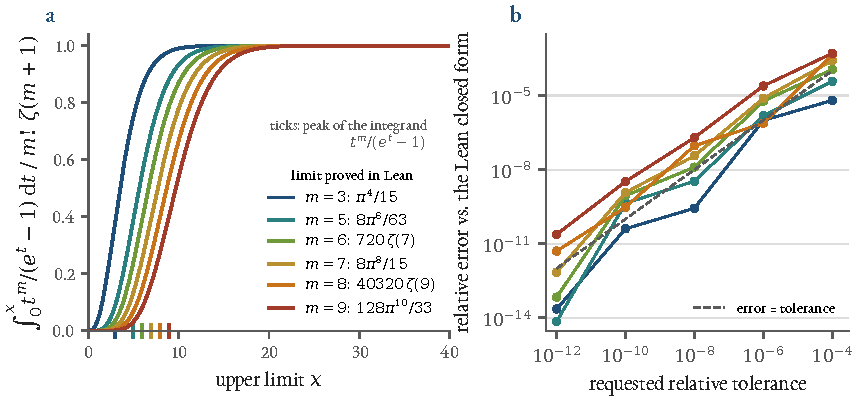
\includegraphics[width=\linewidth]{figures/ch04_bose.pdf}
\caption[The six Bose integrals of the Lean statement, computed by CVODE]{The six Bose integrals of Lean's \lean{bose\_integral\_values} computed by CVODE (Adams). \textbf{(a)} The cumulative integrals $\int_0^x t^m/(e^t-1)\,\mathrm dt$ divided by their limits; the integrand peaks near $t=m$ (ticks), so the higher-order terms of the series draw their weight from higher energies. \textbf{(b)} Relative error against the closed forms proved in Lean, versus the requested relative tolerance; the dashed line is error equal to tolerance.}\label{ch04:fig-bose}
\end{figure}

The largest error is between \cfv{bose-ratio-min} and \cfv{bose-ratio-max} times the requested tolerance over the whole range from $10^{-4}$ to $10^{-12}$ (the global error of a multistep method exceeds its local tolerance); at the tightest tolerance the six closed forms $\pi^4/15$ to $128\pi^{10}/33$ are matched to $\cfv{bose-err-1m12}$ (\cref{ch04:fig-bose}b).
Panel (a) carries a physical point for later: the integrand $t^m/(e^t-1)$ peaks near $t=m$, so the term of order $T^{m}$ draws its weight from phonons of energy about $m\,\cfkB T$, the $L$ term from nine thermal energies, not one: a series in $T$ is a series in progressively less thermal phonons.

\subsection{The thermal integral with no series at all}
Now the experiment that matters.
For the model dispersion, let the solver integrate over wavevector the thermal integral that \emph{defines} the specific heat, with one ODE component per temperature, and compare with the truncated series.
There is one technical step, and it is a use of the first Lean theorem.
Written naively, the answer is of order $A\,T^3$ and the interesting part, the series' corrections, is a small difference of order $T^2$ (relative) hidden inside it; a solver with relative tolerance $10^{-12}$ then sees the corrections only to $10^{-12}$ of the whole.
But the Debye law is \emph{proved}: $\int_0^\infty (V\cfkB/2\pi^2)\,k^2 f(\hbar ck/\cfkB T)\,\mathrm dk=A\,T^3$ exactly (\lean{debye\_specific\_heat}).
So subtract it inside the integrand, and give the solver only the difference:
\begin{align}
 \frac{C_V(T)}{A\,T^3}&=1+\int_0^{k_{\max}}\frac{V\cfkB\,k^2}{2\pi^2\,A\,T^3}\Bigl[f(x_{\rm poly})-f(x_{\rm D})\Bigr]\mathrm dk,\label{ch04:eq-ode}\\
 x_{\rm poly}&=\frac{\hbar c\,k(1+\alpha_2k^2+\alpha_3k^3+\alpha_4k^4)}{\cfkB T},\qquad x_{\rm D}=\frac{\hbar ck}{\cfkB T},\nonumber
\end{align}
with $f(x)=x^2e^x/(e^x-1)^2$ and $k_{\max}=2.5\ \cfAng^{-1}$ (beyond it the Debye integrand contributes less than $10^{-14}$ of $A\,T^3$ for every $T\le1\cfK$).
The right-hand side of the ODE is the integrand of \eqref{ch04:eq-ode} evaluated at all the temperatures at once.

\begin{rustbox}{CVODE: the specific heat of the model dispersion, no series}
\begin{lstlisting}[style=py,basicstyle=\ttfamily\footnotesize]
def rhs_model(k, y):               # one component per temperature in T_all (68 of them)
    if k <= 0.0:
        return [0.0]*len(T_all)
    xp = cc.THETA*cc.u_poly(k)/T_all          # eps/k_B T, polynomial dispersion
    xd = cc.THETA*k/T_all                     # eps/k_B T, Debye dispersion
    return (cc.PREF*k*k*(cc.bose_weight(xp) - cc.bose_weight(xd))/fT(T_all)).tolist()
# excerpt of figures/ch04_cvode_compute.py;  cc.PREF = V k_B/(2 pi^2),  fT(T) = A T^3
y, info = solve_ode(rhs_model, [0.0]*len(T_all), [0.0, cc.KMAX_MODEL],
                    1e-12, 1e-14, "model")
\end{lstlisting}
\noindent \emph{\cfv{nT-all} temperatures (\cfv{nT-log} geometrically spaced from $0.005$ to $1\cfK$, the reference temperature $0.02\cfK$, and the \cfv{nT-lin} of the measured table), Adams, relative tolerance $10^{-12}$, absolute $10^{-14}$ in units of $A\,T^3$: \cfv{model-calls} right-hand-side calls, \cfv{model-seconds} s on the shared 8-core machine at load average about \cfv{model-load}. Against a 30-digit \texttt{mpmath} quadrature of the same integrand at seven temperatures ($0.005$ to $1\cfK$) the absolute error is \cfv{model-abserr-0.1} at $0.1\cfK$ and at most \cfv{model-abserr} (at $0.005\cfK$). Without the subtraction, at the same tolerances: \cfv{model-raw-abserr-0.1} at $0.1\cfK$.}
\end{rustbox}

The subtraction is worth having: at relative tolerance $10^{-8}$ it reduces the absolute error of the result from \cfv{raw8-0.005} to \cfv{sub8-0.005} at $0.005\cfK$ and from \cfv{raw8-0.1} to \cfv{sub8-0.1} at $0.1\cfK$.
The proved Debye law is not decoration here, it is what lets the solver see the series.

\begin{figure}[t]\centering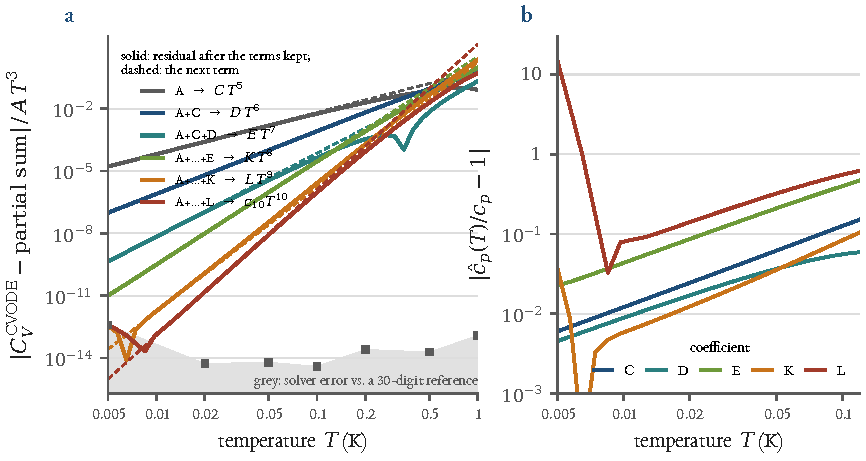
\includegraphics[width=\linewidth]{figures/ch04_ladder.pdf}
\caption[The solver against the proved series]{The solver against the proved series. \textbf{(a)} The absolute difference between the CVODE value of $C_V/A\,T^3$ for the model dispersion and the truncation of Eq.~(22) named on each line, versus $T$ (solid), with the next term of the series (dashed): each line should have the slope of the term it does not contain. The grey squares are the solver's own absolute error, measured against a 30-digit reference at seven temperatures. The top line (only $A$) is Debye's law; the bottom line (after $L$) is compared with a coefficient, $c_{10}$, that Lean does not contain and exact rational arithmetic supplies. \textbf{(b)} The relative error of the coefficient that the numerical data themselves suggest, $\hat c_p(T)=(C_V-\sum_{q<p}c_qT^q)/T^p$ with the coefficients $c_q$ ($q<p$) of Eq.~(22), against $c_p$.}\label{ch04:fig-ladder}
\end{figure}

\Cref{ch04:fig-ladder}a is the test.
If the closed forms are the coefficients, then the residual after $A$ is $C\,T^5(1+O(T))$, that after $A+C$ is $D\,T^6(1+O(T))$, and so on: a ladder of straight lines in logarithmic axes, with slopes $2,3,4,5,6$ (the powers of $T$ minus 3) and a last line of slope $7$.
The lines are straight, and the fitted slopes agree with the expected ones to within about \cfv{slope-maxdev} (the slope of a sum of two power laws is not exactly that of the leading one).
Over the range where each residual lies above a thousand times the solver's error and $T\le0.06\cfK$, fitted slopes against the expected ones are:
\begin{center}\small
\begin{tabular}{@{}lcccccc@{}}\toprule
 truncated after & $A$ & $A{+}C$ & $A{+}C{+}D$ & $\dots{+}E$ & $\dots{+}K$ & $\dots{+}L$\\ \midrule
 next term & $C\,T^5$ & $D\,T^6$ & $E\,T^7$ & $K\,T^8$ & $L\,T^9$ & $c_{10}T^{10}$\\
 expected slope & \cfv{slope-exp-A} & \cfv{slope-exp-AC} & \cfv{slope-exp-ACD} & \cfv{slope-exp-ACDE} & \cfv{slope-exp-ACDEK} & \cfv{slope-exp-ACDEKL}\\
 fitted slope & \cfv{slope-A} & \cfv{slope-AC} & \cfv{slope-ACD} & \cfv{slope-ACDE} & \cfv{slope-ACDEK} & \cfv{slope-ACDEKL}\\
 residual / next term at the lowest $T$ & \cfv{ratio-A} & \cfv{ratio-AC} & \cfv{ratio-ACD} & \cfv{ratio-ACDE} & \cfv{ratio-ACDEK} & \cfv{ratio-ACDEKL}\\ \bottomrule
\end{tabular}
\end{center}
The solid lines meet the dashed ones as $T\to0$: at the lowest temperature of each line the residual is within about 10 per cent of the next term (last row), and the solver's absolute error, in units of $A\,T^3$, is $\cfv{floor-0.1}$ at $0.1\cfK$ (grey squares in the figure).
The absence of a $T^4$ term, the exactness of $A,C,D,E,K$ and the order of $L$ are thus visible in a computation that never used a series.
The one coefficient \emph{not} confirmed by Lean here, $c_{10}$, is confirmed by the solver to the same standard --- as it should be, since exact rational arithmetic computed it.

\subsection{What numerics cannot see}
A solver is blind below its tolerance, and the series makes that blindness worse.
\Cref{ch04:fig-ladder}b asks how well the numerical data alone would determine each coefficient.
The quantity $\hat c_p(T)=(C_V-\sum_{q<p}c_qT^q)/T^p$ tends to $c_p$ as $T\to0$, but only linearly (the first neglected term enters as $c_{p+1}T/c_p$), and the smaller $T$, the more of $\hat c_p$ is solver noise divided by $T^p$.
At $0.02\cfK$, with data whose absolute error in units of $A\,T^3$ is only $\cfv{floor-0.02}$, the coefficients $C,D,E,K,L$ come out with relative errors of $\cfv{rec-0.02-C}$, $\cfv{rec-0.02-D}$, $\cfv{rec-0.02-E}$, $\cfv{rec-0.02-K}$ and $\cfv{rec-0.02-L}$ per cent against the Lean values; at $0.05\cfK$ of $\cfv{rec-0.05-C}$, $\cfv{rec-0.05-D}$, $\cfv{rec-0.05-E}$, $\cfv{rec-0.05-K}$ and $\cfv{rec-0.05-L}$ per cent.
This is the inverse problem of an experimenter who fits $C_V/T^3$ to a polynomial: the forward map from the dispersion to the series is explicit and well conditioned, the inverse map is not.

It also explains why two of the four wrong versions of the previous section could not have been caught numerically.
Replacing $15120$ by $15121$ changes $C_V/A\,T^3$ at $0.1\cfK$ by $\cfv{ctl-D-0.1}$ and replacing $55$ by $54$ by $\cfv{ctl-L-0.1}$, whereas the first term the series does not contain, $c_{10}T^{10}$, contributes $\cfv{ctl-next-0.1}$, that is $\cfv{ctl-D-ratio}$ and $\cfv{ctl-L-ratio}$ times more.
Both effects are far above the solver's error ($\cfv{floor-0.1}$), but cannot be separated from the next term of the series without already knowing it.
The coarser slip $8\alpha_2\alpha_3$ for $9\alpha_2\alpha_3$ in $K$ changes $C_V/A\,T^3$ by $\cfv{ctl-K-0.1}$, $\cfv{ctl-K-ratio}$ times the neighbouring term; it would turn the slope-6 line of \cref{ch04:fig-ladder}a into a line of slope 5, and the solver would catch it.
Lean rejected all of them.
The two instruments are not redundant: the solver sees a whole function, its slopes and gross slips; the proof assistant sees every coefficient to the last digit.


%% ====================================================================================================================
\section{The series meets the measured curve}\label{ch04:sec-data}

Everything so far concerned a \emph{model}, the polynomial \eqref{ch04:eq-disp}.
The specific heat of helium is the integral \eqref{ch04:eq-energy} of the \emph{measured} dispersion.
This section puts the two next to each other, with one rule: nothing is tuned.
The coefficients, $c$ and $V$ are those quoted in the paper, and the dispersion is the open table.

\subsection{Reproducing the paper's table}
The open ancillary files of the paper contain, besides the dispersion, a table of the specific heat from $0.01$ to $1.3\cfK$ with three columns: total, ``phonon'' and ``roton''.
I recomputed it from the dispersion table with CVODE: the table interpolated by a cubic spline in $k$, the thermal integral written as an initial-value problem in $k$ with one component per temperature (as in Section~\ref{ch04:sec-solver}), integrated first to the maxon wavevector $k_M=\cfv{maxon-k}\ \cfAng^{-1}$ (the maximum of the table's $\varepsilon(k)$: the phonon column) and then to the end of the table at $3.6\ \cfAng^{-1}$ (the total), for the \cfv{n-T} temperatures $0.05,0.10,\dots,1.30\cfK$.
Adams, relative tolerance $10^{-8}$, absolute $10^{-11}$ in units of $A\,T^3$; \cfv{repro-calls} right-hand-side evaluations in about \cfv{repro-seconds} s on the shared machine (load average $\approx\cfv{repro-load}$).
Against the tabulated total the relative difference is at worst $\cfv{repro-max}$ (at $\cfv{repro-T-of-max}\cfK$) and \cfv{repro-median} in the median; the phonon column agrees to $\cfv{repro-ph-max}$; SciPy's adaptive quadrature gives the same integral as CVODE to $\cfv{repro-vs-quad}$.
The table carries four significant digits, which would show differences of order $10^{-4}$; the larger differences are real but small compared with the table's own uncertainty column ($\cfv{paper-unc-0.7}$ per cent at $0.7\cfK$), and I did not track them down (the interpolation between grid points and the treatment of the ultrasound-based region below $0.15\ \cfAng^{-1}$ are candidates).
It is a reproduction of a tabulated number from its own open data, nothing more; but it tells us that the integral computed below is the same quantity as the table's.

\subsection{Which excitations carry the heat}
\begin{figure}[t]\centering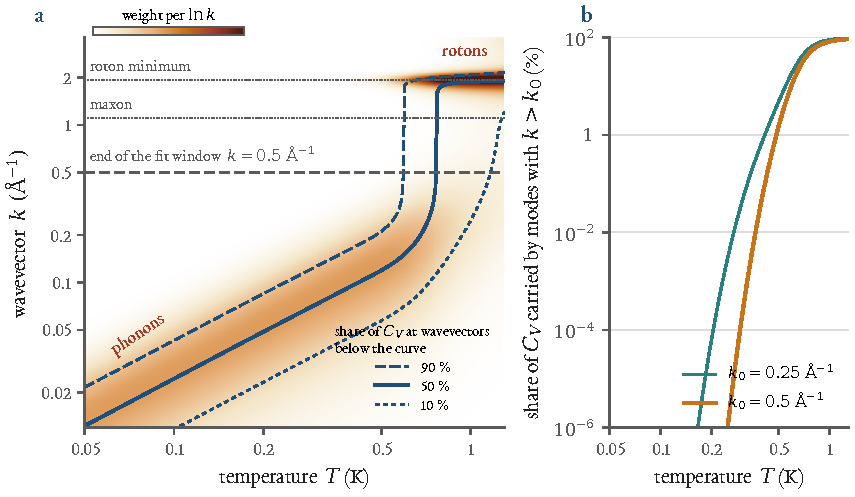
\includegraphics[width=\linewidth]{figures/ch04_heatmap.pdf}
\caption[Which excitations carry the heat?]{Which excitations carry the heat? \textbf{(a)} The distribution of the specific heat over the wavevector $k$ of the excitation, $w(k,T)=\bigl(V\cfkB/2\pi^2\bigr)k^2 f(\varepsilon/\cfkB T)/C_V(T)$ with $f(x)=x^2e^x/(e^x-1)^2$, per unit $\ln k$, computed from the measured dispersion table (integration limit $3.6\ \cfAng^{-1}$); white is no weight. The phonon ridge climbs along $k\propto T$; at about $0.8\cfK$ the median wavevector jumps to the roton minimum. Curves: wavevectors below which 10, 50 and 90 per cent of $C_V$ sit. \textbf{(b)} The share of $C_V$ carried by modes with $k>k_0$, for $k_0=0.25$ and $0.5\ \cfAng^{-1}$.}\label{ch04:fig-heatmap}
\end{figure}

\Cref{ch04:fig-heatmap} is built from the same table.
It shows the structure that the series ignores.
At $0.1\cfK$ half of the specific heat is carried by phonons with $k<\cfv{med-k-0.1}\ \cfAng^{-1}$, wavelengths longer than $\cfv{lambda-0.1}\ \cfAng$, and nine tenths by $k<\cfv{q90-k-0.1}\ \cfAng^{-1}$; at $0.5\cfK$ the numbers are $\cfv{med-k-0.5}$ and $\cfv{q90-k-0.5}\ \cfAng^{-1}$.
The ridge is a straight line of unit slope in these logarithmic axes, as the Debye law says ($k\propto T$), bending slowly because $\alpha_2>0$.
Then the weight switches: in my integration the roton part of the integral overtakes the phonon part at $\cfv{T-cross}\cfK$, and the median wavevector jumps to the roton minimum at $k=\cfv{roton-k}\ \cfAng^{-1}$.
Panel (b) quantifies what the polynomial's range of validity would suggest.
If the polynomial is only trusted below $0.5\ \cfAng^{-1}$, the fraction of the specific heat that falls outside it is $\cfv{share05-0.3}$ per cent at $0.3\cfK$, $\cfv{share05-0.5}$ per cent at $0.5\cfK$, $\cfv{share05-0.7}$ per cent at $0.7\cfK$ and $\cfv{share05-1.0}$ per cent at $1\cfK$.
So by this criterion the polynomial should serve almost to $0.5\cfK$ and fail within a few tenths of a kelvin above.
We now see whether the series does.

\subsection{An error budget}
\begin{figure}[t]\centering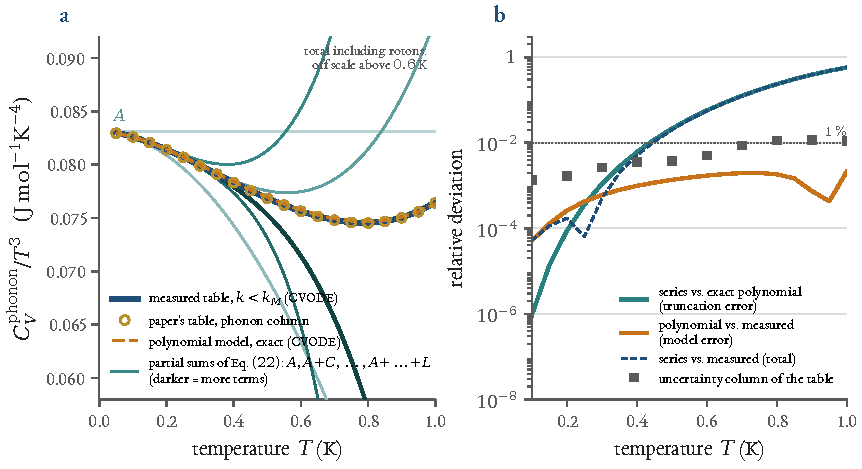
\includegraphics[width=\linewidth]{figures/ch04_budget.pdf}
\caption[Eq.~(22) against the integral of the measured dispersion]{Eq.~(22) against the integral of the measured dispersion. \textbf{(a)} $C_V/T^3$ of the phonon part ($k<k_M$): the integral of the measured table (blue, CVODE), the paper's own table column (circles), the exact integral of the polynomial model (orange dashed, CVODE), and the partial sums of Eq.~(22) (teal, darkening with the number of terms). The total including rotons rises above the frame beyond $0.6\cfK$. \textbf{(b)} Three relative deviations: the six-term series against the exact integral of the \emph{same} polynomial (the series' own truncation error, teal); that polynomial against the measured table (the model error, orange); the series against the measured table (the total, blue dashed). Grey squares: the uncertainty column of the paper's table, relative to its total $C_V$.}\label{ch04:fig-budget}
\end{figure}

\Cref{ch04:fig-budget} separates two sources of error that are usually mixed.
The six-term series is an approximation to the integral of the polynomial, and the polynomial is an approximation to helium.
The solver gives the exact integral of the polynomial, so the two can be told apart.
Up to about $0.3\cfK$ everything is excellent: the series differs from the exact polynomial integral by $\cfv{bud-trunc-pct-0.3}$ per cent at $0.3\cfK$, and the polynomial differs from the measured phonon integral by $\cfv{bud-model-pct-0.3}$ per cent.
At $0.5\cfK$ the picture has changed: the model error is $\cfv{bud-model-pct-0.5}$ per cent and the truncation error of the six terms is $\cfv{bud-trunc-pct-0.5}$ per cent, more than a factor of ten larger.
At $0.7\cfK$ the truncation error has reached $\cfv{bud-trunc-pct-0.7}$ per cent; above that the series is useless as an approximation.
The six-term series first departs from the exact polynomial integral by more than one per cent at $\cfv{bud-first_T_series6_vs_poly_exceeds_1pct}\cfK$.
For scale, the uncertainty column of the paper's table is $\cfv{paper-unc-0.1}$ per cent of the total at $0.1\cfK$, $\cfv{paper-unc-0.3}$ per cent at $0.3\cfK$ and $\cfv{paper-unc-0.5}$ per cent at $0.5\cfK$ (grey squares).
So the limit on the series is not the polynomial's range of validity, as the heat map suggested --- at $0.5\cfK$ only $\cfv{share05-0.5}$ per cent of the heat is carried outside it --- but the \emph{series} itself: as a series in $T$ it runs out of accuracy earlier than the model it expands.

\subsection{A series that does not converge}
\begin{figure}[t]\centering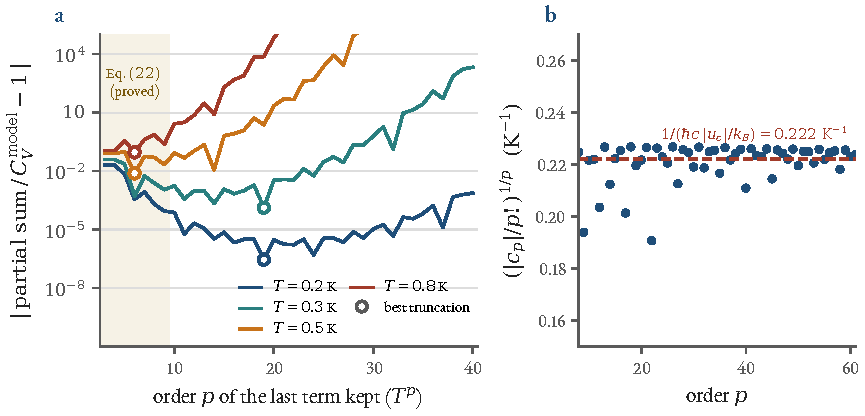
\includegraphics[width=\linewidth]{figures/ch04_asymptotic.pdf}
\caption[The series is asymptotic, not convergent]{The series continues to every order and is asymptotic, not convergent. \textbf{(a)} Relative error of the partial sum through $T^p$ against the exact (CVODE) integral of the polynomial model, for four temperatures, with the coefficients of Eq.~(22) and beyond from exact rational arithmetic; circles mark the best truncation. The gold band is the range proved in Lean. \textbf{(b)} The root test $(|c_p|/p!)^{1/p}$ of the coefficients $c_p$ of $T^p$; the dashed line is $1/(\hbar c|u_c|/\cfkB)$, computed from the critical points of $u(k)$ alone.}\label{ch04:fig-asymptotic}
\end{figure}

The exact-rational script of Section~\ref{ch04:sec-confirm} does not stop at $L$.
For the paper's coefficient set the coefficients of $T^p$ for $p=3,5,6,7,8,9$ are, relative to $A$: $1$, $\cfv{rA-5}$, $\cfv{rA-6}$, $\cfv{rA-7}$, $\cfv{rA-8}$, $\cfv{rA-9}$, and the next ones, beyond Lean, are $\cfv{rA-10}$ ($p=10$), $\cfv{rA-11}$, $\cfv{rA-12}$, $\cfv{rA-13}$, $\cfv{rA-14}$, growing.
\Cref{ch04:fig-asymptotic}a shows the consequence.
At $T=0.2\cfK$ the error of the partial sum falls as terms are added, reaches $\cfv{best-err-0.2}$ at order $p=\cfv{best-order-0.2}$, and then grows without bound; at $0.3\cfK$ the best is $\cfv{best-err-0.3}$ (order $\cfv{best-order-0.3}$); at $0.5\cfK$ it is $\cfv{best-err-0.5}$ (order $\cfv{best-order-0.5}$); at $0.8\cfK$ it is $\cfv{best-err-0.8}$ (order $\cfv{best-order-0.8}$).
So the six terms of Eq.~(22), through $T^9$, stop well short of the best truncation at $0.2$ and $0.3\cfK$, and overshoot it from $0.5\cfK$ on: at $0.5\cfK$ the error after $A+C+D$ ($T^6$) is $\cfv{best-err-0.5}$, smaller than the $\cfv{err9-0.5}$ after all six terms.
The six terms of Eq.~(22) are the beginning of an \emph{asymptotic} expansion, not of a convergent one that could be extended at will; its best truncation depends on the temperature.

Where does the divergence come from?
Two factors.
The Bose integrals contribute $(n+2)!$ to the coefficient of $T^{n+1}$ (they are $\Gamma$ functions), a factorial.
And the density of states $g(u)=\sum g_nu^n$ has a finite radius of convergence: $k(u)$ is the inverse function of $u(k)$ and has a branch point at every critical value of $u(k)$, where $\mathrm du/\mathrm dk=0$, so $g_n$ grows like $R^{-n}$ with $R$ the distance from the origin to the nearest singularity on the principal sheet.
The polynomial $u(k)=k(1+\alpha_2k^2+\alpha_3k^3+\alpha_4k^4)$ has degree five, so $\mathrm du/\mathrm dk=0$ is a quartic equation, with two complex-conjugate pairs of roots; the pair with the smaller critical value sits at $k_c=\cfv{uc-k-re}\pm\cfv{uc-k-im}\,i\ \cfAng^{-1}$ and gives $u_c=\cfv{uc-u-re}\pm\cfv{uc-u-im}\,i\ \cfAng^{-1}$, $|u_c|=\cfv{uc-abs}\ \cfAng^{-1}$, that is an energy $\hbar c|u_c|/\cfkB=\cfv{uc-K}\cfK$.
Together: the coefficient of $T^p$ behaves like $p!\,(\hbar c|u_c|/\cfkB)^{-p}$, and the root test $(|c_p|/p!)^{1/p}$ should tend to $1/(\hbar c|u_c|/\cfkB)=\cfv{uc-inv}\ \mathrm{K^{-1}}$.
\Cref{ch04:fig-asymptotic}b shows that it does: the sequence is $\cfv{root-p20}$ at $p=20$, $\cfv{root-p40}$ at $p=40$ and $\cfv{root-p60}$ at $p=60$.
The same reasoning gives the optimal order, where the factorial overtakes the geometric decay, $p^\ast\approx\hbar c|u_c|/\cfkB T$, and the best accuracy, $\exp(-\hbar c|u_c|/\cfkB T)$ times a power of $T$.
The order $p^\ast$ at which the terms (taken as the largest of three consecutive ones, to suppress accidental zeros) are smallest is $\cfv{pstar-0.1}$ at $0.1\cfK$ (the estimate gives $\cfv{pstar-pred-0.1}$), $\cfv{pstar-0.2}$ at $0.2\cfK$ ($\cfv{pstar-pred-0.2}$), $\cfv{pstar-0.3}$ at $0.3\cfK$ ($\cfv{pstar-pred-0.3}$) and $\cfv{pstar-0.4}$ at $0.4\cfK$ ($\cfv{pstar-pred-0.4}$); and fitting the size of those smallest terms for $\cfv{fit-T-lo}\le T\le\cfv{fit-T-hi}\cfK$ to $a\,T^s e^{-b/T}$ gives $b=\cfv{fit-b}\cfK$ and $s=\cfv{fit-s}$, against the predicted $b=\cfv{fit-b-pred}\cfK$.
The $\cfv{uc-K}\cfK$ scale is a property of the \emph{polynomial} --- the complex critical points are an artefact of truncating the dispersion at $\alpha_4$ --- and not of helium, whose measured dispersion has a real maxon at $\varepsilon/\cfkB=\cfv{maxon-K}\cfK$ and a roton minimum at $\cfv{roton-K}\cfK$; it is an illustration of how a truncated polynomial and a Bose integral conspire, not a statement about the real fluid.
What the figure says is limited: below about $0.3\cfK$ the six-term series represents the integral of the polynomial excellently, above $0.5\cfK$ it does not, and the transition is set by the mathematics of the series, not by the measured curve.


%% ====================================================================================================================
\section{What this chapter establishes, and what it does not}\label{ch04:sec-honest}

\begin{honestbox}
\textbf{Proved in Lean (statements about mathematics).}
(i) $\int_0^\infty t^n/(e^t-1)\,\mathrm dt=n!\,\zeta(n+1)$ for all $n\ge1$, and its six values at $s=4,6,7,8,9,10$.
(ii) The inverse series printed in the paper inverts $u=k(1+\alpha_1k+\dots+\alpha_6k^6)$ modulo $u^8$, and $k^2\,\mathrm dk/\mathrm du$ equals the density-of-states polynomial modulo $u^9$.
(iii) The derivative with respect to $T$ of the term-by-term energy is the six closed forms $A,C,D,E,K,L$ of Eq.~(22).
(iv) New in this book: the density-of-states brackets are literally the coefficients of $k^2\cdot k'$, with $k'$ the formal derivative, and the capstone can be stated with them and with the Mellin transforms, nothing retyped, and with the energy of each monomial written as its integral (Section~\ref{ch04:sec-newlean}).

\textbf{Derived independently, not in Lean.} The same coefficients by computer algebra, and by exact rational arithmetic, which also gives the terms beyond $L$.

\textbf{Computed here with rusty-SUNDIALS (CVODE, Adams, commit \cfv{rs-commit-short}).} The Bose integrals to the tolerance requested; the specific heat of the model dispersion with no series, whose residual after each truncation has the slope of the next term; the integral of the measured dispersion table, reproducing the paper's table to $\cfv{repro-max}$ (relative, maximum over $0.05$--$1.3\cfK$).

\textbf{Measured by others and used as given.} The dispersion relation $\varepsilon(k)$ (neutron scattering, open ancillary data) and the paper's numerical specific heat, which is itself an integral of that dispersion. I did not measure anything, and I did not compare with calorimetry: the calorimetric data are not in the open files.

\textbf{Not established, and not claimed.}
(a) That Eq.~(22) describes liquid helium at any temperature: it is a statement about the polynomial \eqref{ch04:eq-disp}. Section~\ref{ch04:sec-data} shows what the six terms do, for the model and against the table.
(b) That the series converges: for the model it does not, and the divergence is computed here, not proved in Lean. The legitimacy of term-by-term integration, and the asymptotic character of the expansion for a measured curve, are analytical statements that the library does not contain.
(c) Anything about $\alpha_1\ne0$ (the $T^4$ term and the $\alpha_1$-dependence of the other coefficients): the Lean files treat $C_V$ for $\alpha_1=0$ only.
(d) Anything about errata in the paper. The check found no discrepancy between the printed closed forms and the derived ones; the formulas checked are those of the arXiv version, and the version of record was not compared.
(e) The picture of a gas of non-interacting phonons, and the density of states $V k^2\mathrm dk/2\pi^2$, are modelling assumptions of the physics; no theorem here proves that liquid helium is such a gas.

\textbf{What failed or was left unexplained.}
The first version of the new Lean file forgot \lean{open Real}: Lean then read \lean{π} as a fresh variable (an auto-bound implicit), and the capstone failed with a type mismatch between that variable and \lean{Real.pi} --- the checker rejecting a statement about the wrong object, as it should.
My first runs used a stale build of the solver, whose Adams method was implicit Euler: plausible numbers, wrong by up to hundreds of times the tolerance; they were discarded, and every number of the chapter was recomputed with the fixed build (Section~\ref{ch04:sec-solver}).
The derivation check of 2026-09-21 was not pre-registered; the design note records that lapse.
\end{honestbox}

%% ====================================================================================================================
\section*{Exercises}\addcontentsline{toc}{section}{Exercises}

\paragraph{Exercise 1.}
\emph{The missing $T^4$ term.} Keep $\alpha_1\neq0$ and set $\alpha_2=\alpha_3=\dots=0$, so that $\varepsilon=\hbar ck(1+\alpha_1k)$.
(a) Invert $u=k(1+\alpha_1k)$ exactly and show that the density of states is $k^2\,\mathrm dk/\mathrm du=u^2-4\alpha_1u^3+15\alpha_1^2u^4-56\alpha_1^3u^5+\dots$.
(b) Use \eqref{ch04:eq-series} with $n=3$ to show that $C_V$ acquires a term $B\,T^4$ with $B=-240\,\zeta(5)\,\alpha_1\,V\cfkB^5/(\pi^2\hbar^4c^4)$.
(c) Explain why Eq.~(22) has no such term, and which line of \lean{density\_of\_states} is the $T^4$ term's absence.\\
\emph{Hint.} (a) $k=(-1+\sqrt{1+4\alpha_1u})/2\alpha_1$, and $g=\mathrm d(k^3/3)/\mathrm du$. (b) The factor is $(n+2)!\,\zeta(n+2)=5!\,\zeta(5)$ and $g_3=-4\alpha_1$. (c) $g_3=0$ when $\alpha_1=0$; the missing $e^3$ in the right-hand side. The expression in (b) agrees with the $B$ printed for $\alpha_1\ne0$ in the Supplemental Material of the arXiv version of the paper; the Lean files do not cover it.

\paragraph{Exercise 2.}
\emph{Where do $5$, $28$, $165$ come from?} Set $\alpha_3=\alpha_4=\alpha_5=\alpha_6=0$.
Show, by Lagrange inversion, that $g_{2n+2}=(-1)^n\binom{3n+2}{n}\alpha_2^n$.
Check it against the brackets of $C$, $E$ and $L$ ($-5$, $28=7\cdot4$, $-165=-3\cdot55$), and predict the coefficient $1001\,\alpha_2^4$ of $u^{10}$.\\
\emph{Hint.} For $u=k(1+\alpha_2k^2)$ one has $[u^m]\,k^r=\tfrac rm\,[k^{m-r}]\,(1+\alpha_2k^2)^{-m}$. Take $r=3$, $m=2n+3$, and note $g_{2n+2}=\tfrac{2n+3}3\,[u^{2n+3}]\,k^3$. (The formula was checked symbolically through $n=4$ while writing this chapter.)

\paragraph{Exercise 3.}
\emph{Optimal truncation.} At fixed $T$ the terms $c_pT^p$ of the series \eqref{ch04:eq-series} first shrink and then grow.
Using $(|c_p|/p!)^{1/p}\to1/(\hbar c|u_c|/\cfkB)$ with $\hbar c|u_c|/\cfkB=\cfv{uc-K}\cfK$ (Section~\ref{ch04:sec-data}), show that the smallest term sits near $p^\ast\approx\cfv{uc-K}\cfK/T$ and that the best accuracy of the truncated series is of order $\exp(-\cfv{uc-K}\cfK/T)$ up to a power of $T$.
Compare with \cref{ch04:fig-asymptotic} and Section~\ref{ch04:sec-data}: at $T=0.2\cfK$ the smallest terms sit at order $\cfv{pstar-0.2}$ while the estimate gives $\cfv{pstar-pred-0.2}$.\\
\emph{Hint.} Stirling: $\ln(p!\,x^p)\approx p\ln(px/e)$ with $x=T/\cfv{uc-K}\cfK$; minimize over $p$.

%% ====================================================================================================================
\section*{Notes and further reading}\addcontentsline{toc}{section}{Notes and further reading}

The phonon--roton spectrum is Landau's \cite{Landau1941}; textbook accounts of the quasiparticle picture are in \cite{PitaevskiiStringari2016,Donnelly1991}.
The measurement and the analytical and numerical thermodynamics of this chapter are those of Godfrin and collaborators \cite{Godfrin2021}; the wider survey of excitation spectra of quantum fluids is \cite{GodfrinKrotscheck2022}.
Calorimetric determinations of the phonon dispersion of liquid $^4$He are \cite{Phillips1970,Greywall1978}.
For asymptotic series and the idea of optimal truncation (Section~\ref{ch04:sec-data}) see \cite{BenderOrszag1999}.
The Lean library is \cite{Callens2026lib}, built on Mathlib \cite{Mathlib2020} and Lean~4 \cite{deMoura2021}; the history of the three modules, including the derivation script and the generator of the certificates, is in \texttt{docs/designs/PHONON\_SERIES\_A\_TO\_L.md} of the repository.
The solver is CVODE of the SUNDIALS family \cite{Hindmarsh2005}, in its rusty-SUNDIALS port.
Every figure is made by a script \texttt{figures/ch04\_*.py} from \texttt{ch04\_cvode\_raw.json}, \texttt{ch04\_cvode\_results.npz} and \texttt{ch04\_numbers.json}; every computed number in the text is read from the last of these by \texttt{figures/ch04\_numbers\_tex.py}.
}
\IfCh{ch05}{\chapter{Phonons, Rotons and the Dispersion Relation}\label{ch05}
% generated by ch05_numbers.py -- do not edit
\expandafter\def\csname cfive@tableRows\endcsname{1\,727}
\expandafter\def\csname cfive@nErrRows\endcsname{34}
\expandafter\def\csname cfive@kmax\endcsname{3.6}
\expandafter\def\csname cfive@c\endcsname{238.3}
\expandafter\def\csname cfive@kDense\endcsname{3.44}
\expandafter\def\csname cfive@maxonKshort\endcsname{1.1}
\expandafter\def\csname cfive@maxonE\endcsname{1.19}
\expandafter\def\csname cfive@rotonE\endcsname{0.741}
\expandafter\def\csname cfive@rotonGapK\endcsname{8.60}
\expandafter\def\csname cfive@rotonKshort\endcsname{1.92}
\expandafter\def\csname cfive@rotonMass\endcsname{0.141}
\expandafter\def\csname cfive@landauV\endcsname{57.9}
\expandafter\def\csname cfive@landauK\endcsname{1.97}
\expandafter\def\csname cfive@landauOverC\endcsname{0.243}
\expandafter\def\csname cfive@landauQuad\endcsname{57.9}
\expandafter\def\csname cfive@landauQuadPct\endcsname{0.01}
\expandafter\def\csname cfive@phaseMaxPct\endcsname{5.4}
\expandafter\def\csname cfive@vphLow\endcsname{238.5}
\expandafter\def\csname cfive@phaseMaxPctAlt\endcsname{5.3}
\expandafter\def\csname cfive@phaseMaxK\endcsname{0.35}
\expandafter\def\csname cfive@kGroup\endcsname{0.404}
\expandafter\def\csname cfive@kSym\endcsname{0.455}
\expandafter\def\csname cfive@kPhase\endcsname{0.566}
\expandafter\def\csname cfive@kSymTable\endcsname{0.453}
\expandafter\def\csname cfive@shiftG\endcsname{0.002}
\expandafter\def\csname cfive@shiftP\endcsname{0.005}
\expandafter\def\csname cfive@symMax\endcsname{14.5}
\expandafter\def\csname cfive@symMaxK\endcsname{0.31}
\expandafter\def\csname cfive@seriesDevMax\endcsname{2.2}
\expandafter\def\csname cfive@kstar\endcsname{3.00}
\expandafter\def\csname cfive@alphaBog\endcsname{0.055}
\expandafter\def\csname cfive@alphaRatio\endcsname{28}
\expandafter\def\csname cfive@h2m4\endcsname{0.522}
\expandafter\def\csname cfive@resFWHM\endcsname{0.07}
\expandafter\def\csname cfive@nPixBin\endcsname{70}
\expandafter\def\csname cfive@err03ueV\endcsname{1.0}
\expandafter\def\csname cfive@bend03ueV\endcsname{23}
\expandafter\def\csname cfive@rotonYat\endcsname{0.25}
\expandafter\def\csname cfive@vgMax\endcsname{1.08}
\expandafter\def\csname cfive@vgMaxPct\endcsname{8.5}
\expandafter\def\csname cfive@vgMaxK\endcsname{0.27}
\expandafter\def\csname cfive@vgCrossK\endcsname{0.40}
\expandafter\def\csname cfive@vgZeroK\endcsname{1.10}
\expandafter\def\csname cfive@vgMin\endcsname{-0.57}
\expandafter\def\csname cfive@vgMinK\endcsname{1.63}
\expandafter\def\csname cfive@exLandau\endcsname{58.0}
\expandafter\def\csname cfive@mfMaxK\endcsname{0.56}
\expandafter\def\csname cfive@mfMaxW\endcsname{0.350}
\expandafter\def\csname cfive@mfMinK\endcsname{0.84}
\expandafter\def\csname cfive@mfMinW\endcsname{0.304}
\expandafter\def\csname cfive@mfLandau\endcsname{0.349}
\expandafter\def\csname cfive@mfLandauK\endcsname{0.90}
\expandafter\def\csname cfive@pLandau0\endcsname{57.9}
\expandafter\def\csname cfive@pLandau24\endcsname{46.1}
\expandafter\def\csname cfive@pRatio0\endcsname{0.243}
\expandafter\def\csname cfive@pRatio24\endcsname{0.127}
\expandafter\def\csname cfive@pC24\endcsname{362}
\expandafter\def\csname cfive@pCrise\endcsname{52}
\expandafter\def\csname cfive@pRoton24\endcsname{0.626}
\expandafter\def\csname cfive@pKR24\endcsname{2.05}
\expandafter\def\csname cfive@pP24\endcsname{24.08}
\expandafter\def\csname cfive@pKmaxRange\endcsname{2.2}
\expandafter\def\csname cfive@nModesMain\endcsname{3208}
\expandafter\def\csname cfive@nmodesRetained\endcsname{3209}
\expandafter\def\csname cfive@nModesG2\endcsname{796}
\expandafter\def\csname cfive@Tmain\endcsname{300}
\expandafter\def\csname cfive@nGolden\endcsname{28}
\expandafter\def\csname cfive@secRun\endcsname{65}
\expandafter\def\csname cfive@secFit\endcsname{12}
\expandafter\def\csname cfive@medMain\endcsname{0.60}
\expandafter\def\csname cfive@p99Main\endcsname{8.5}
\expandafter\def\csname cfive@maxMain\endcsname{26}
\expandafter\def\csname cfive@medG2\endcsname{0.42}
\expandafter\def\csname cfive@medSplit\endcsname{1.2}
\expandafter\def\csname cfive@medLowK\endcsname{3.8}
\expandafter\def\csname cfive@medHighK\endcsname{0.33}
\expandafter\def\csname cfive@nBand\endcsname{3128}
\expandafter\def\csname cfive@zMin\endcsname{-0.976}
\expandafter\def\csname cfive@zMax\endcsname{-0.488}
\expandafter\def\csname cfive@zDev\endcsname{0.009}
\expandafter\def\csname cfive@ladA\endcsname{\ensuremath{3.6\times10^{-7}}}
\expandafter\def\csname cfive@ladB\endcsname{\ensuremath{2.3\times10^{-8}}}
\expandafter\def\csname cfive@ladC\endcsname{\ensuremath{1.4\times10^{-9}}}
\expandafter\def\csname cfive@ratioA\endcsname{15.6}
\expandafter\def\csname cfive@ratioB\endcsname{16.8}
\expandafter\def\csname cfive@ladVsFit\endcsname{26}
\expandafter\def\csname cfive@collapseA\endcsname{\ensuremath{2.6\times10^{-5}}}
\expandafter\def\csname cfive@collapseB\endcsname{\ensuremath{1.7\times10^{-5}}}
\expandafter\def\csname cfive@labK\endcsname{1.571}
\expandafter\def\csname cfive@labOmega\endcsname{1.9974}
\expandafter\def\csname cfive@labPeakA\endcsname{-2.9975}
\expandafter\def\csname cfive@labPeakB\endcsname{0.9974}
\expandafter\def\csname cfive@labExpA\endcsname{-2.9974}
\expandafter\def\csname cfive@labExpB\endcsname{0.9974}
\expandafter\def\csname cfive@ampK1\endcsname{0.393}
\expandafter\def\csname cfive@ampK2\endcsname{1.571}
\expandafter\def\csname cfive@ampS1\endcsname{\ensuremath{-2.7\times10^{-5}}}
\expandafter\def\csname cfive@ampS2\endcsname{\ensuremath{-2.6\times10^{-3}}}
\expandafter\def\csname cfive@ampS3\endcsname{\ensuremath{-2.2\times10^{-2}}}
\expandafter\def\csname cfive@ampS3pct\endcsname{2.2}
\expandafter\def\csname cfive@ampR1\endcsname{0.19}
\expandafter\def\csname cfive@unkMain\endcsname{6\,418}
\expandafter\def\csname cfive@relSys\endcsname{2.1\times10^{-3}}
\expandafter\def\csname cfive@phaseMaxRatio\endcsname{1.054}
\expandafter\def\csname cfive@vgKcut\endcsname{3.19}
\expandafter\def\csname cfive@ringRmin\endcsname{11}
\expandafter\def\csname cfive@ringRmax\endcsname{28}
\expandafter\def\csname cfive@ringKmin\endcsname{0.8}
\expandafter\def\csname cfive@ringKmax\endcsname{3.1}
\expandafter\def\csname cfive@ringMed\endcsname{3.4}
\expandafter\def\csname cfive@ringMax\endcsname{13}
\expandafter\def\csname cfive@cvN\endcsname{16}
\expandafter\def\csname cfive@cvModes\endcsname{49}
\expandafter\def\csname cfive@cvUnknowns\endcsname{98}
\expandafter\def\csname cfive@cvT\endcsname{20}
\expandafter\def\csname cfive@cvRustSec\endcsname{0.3}
\expandafter\def\csname cfive@cvRk4Dt\endcsname{\ensuremath{5.3\times10^{-7}}}
\expandafter\def\csname cfive@cvEta\endcsname{10^{-4}}
\expandafter\def\csname cfive@cvErr4\endcsname{\ensuremath{7.8\times10^{-4}}}
\expandafter\def\csname cfive@cvErr6\endcsname{\ensuremath{2.7\times10^{-5}}}
\expandafter\def\csname cfive@cvErr8\endcsname{\ensuremath{2.7\times10^{-7}}}
\expandafter\def\csname cfive@cvErr10\endcsname{\ensuremath{3.3\times10^{-9}}}
\expandafter\def\csname cfive@cvBogMax\endcsname{\ensuremath{3.3\times10^{-4}}}
\expandafter\def\csname cfive@cvPerMin\endcsname{1.3}
\expandafter\def\csname cfive@cvPerMax\endcsname{6.4}
\expandafter\def\csname cfive@cvFineErr\endcsname{\ensuremath{2.1\times10^{-9}}}
\expandafter\def\csname cfive@cvBestTol\endcsname{\ensuremath{10^{-10}}}
\expandafter\def\csname cfive@cvBestErr\endcsname{\ensuremath{3.3\times10^{-9}}}
\expandafter\def\csname cfive@cvBestTraj\endcsname{\ensuremath{8.0\times10^{-7}}}
\expandafter\def\csname cfive@cvScale8\endcsname{365}
\expandafter\def\csname cfive@cvScale16\endcsname{710}
\expandafter\def\csname cfive@cvScale32\endcsname{2\,291}
\expandafter\def\csname cfive@cvScaleSec8\endcsname{0.2}
\expandafter\def\csname cfive@cvScaleSec16\endcsname{0.5}
\expandafter\def\csname cfive@cvScaleSec32\endcsname{9.4}
\expandafter\def\csname cfive@cvScaleUnk8\endcsname{26}
\expandafter\def\csname cfive@cvScaleUnk16\endcsname{98}
\expandafter\def\csname cfive@cvScaleUnk32\endcsname{394}
\expandafter\def\csname cfive@unkRatio\endcsname{16}
\expandafter\def\csname cfive@cvSmallN\endcsname{8}
\expandafter\def\csname cfive@cvGrowOldA\endcsname{7}
\expandafter\def\csname cfive@cvGrowOldB\endcsname{9}
\expandafter\def\csname cfive@cvOldFallA\endcsname{11}
\expandafter\def\csname cfive@cvOldFallB\endcsname{10}
\expandafter\def\csname cfive@cvOldDate\endcsname{26 September 2026}
\expandafter\def\csname cfive@cvRatio4\endcsname{2}
\expandafter\def\csname cfive@cvRatio6\endcsname{14}
\expandafter\def\csname cfive@cvOldErr6\endcsname{\ensuremath{1.7\times10^{-3}}}
\expandafter\def\csname cfive@cvNewErr6\endcsname{\ensuremath{1.7\times10^{-5}}}
\expandafter\def\csname cfive@cvRatio8\endcsname{92}
\expandafter\def\csname cfive@nAxiomLines\endcsname{15}

\providecommand{\cfiveV}[1]{\ifcsname cfive@#1\endcsname\csname cfive@#1\endcsname\else\textbf{??#1??}\PackageWarning{ch05}{undefined number key #1}\fi}
\providecommand{\cfiveAng}{\text{\AA}}
\providecommand{\cfivepath}[1]{{\urlstyle{tt}\path{#1}}}

%% ====================================================================================================================
\section{A curve read off a spectrometer}\label{ch05:sec-curve}

Keep a cell of liquid helium below a tenth of a kelvin, send cold neutrons of known energy through it, and note which of them come out having left energy behind.
A neutron that has created exactly one excitation of the liquid --- one phonon, one roton --- is found to have lost a definite energy $\varepsilon$ while its direction changed by an amount that fixes a definite momentum transfer $\hbar k$.
Plot the number of such neutrons against $(k,\varepsilon)$ and, at these temperatures, you get a thin bright line.
That line \emph{is} the dispersion relation of the liquid: the energy of the one-excitation states as a function of their wave number.
Godfrin and his collaborators measured it for superfluid $^4$He on the time-of-flight spectrometer IN5 at the Institut Laue--Langevin \cite{Godfrin2021}, and the authors' processed curve is distributed with the paper as an open table of \cfiveV{tableRows} rows (\cfiveV{nErrRows} of them with an uncertainty), one every $0.002\ \cfiveAng^{-1}$ up to $\cfiveV{kDense}\ \cfiveAng^{-1}$ and four sparser entries out to $\cfiveV{kmax}\ \cfiveAng^{-1}$.
\Cref{ch05:fig-curve}a plots it.

\begin{figure}[tp]
\centering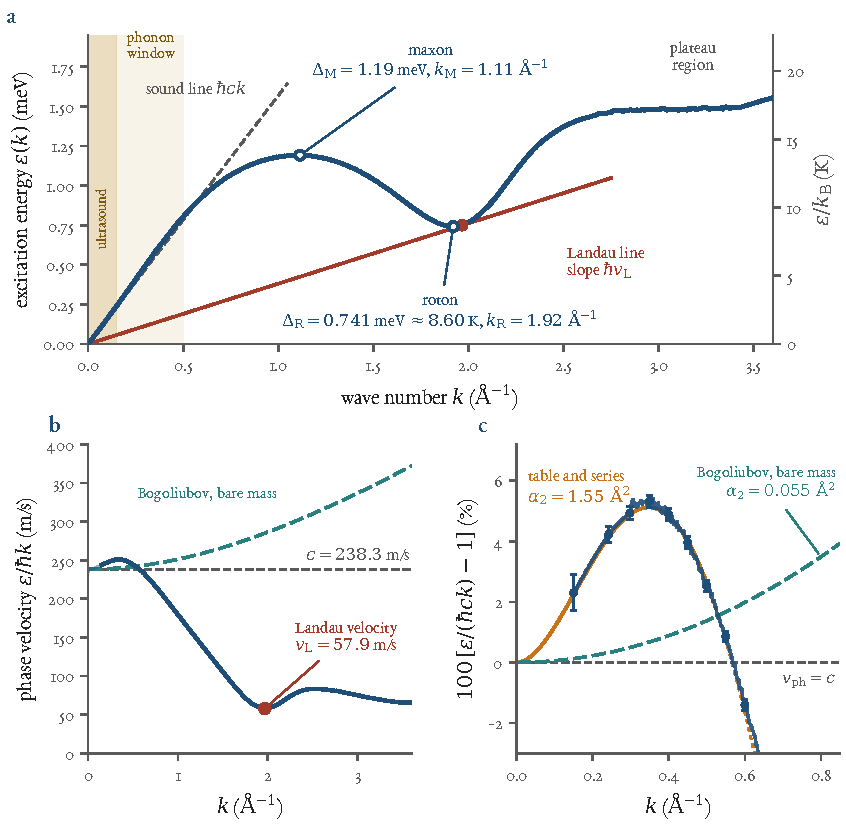
\includegraphics[width=\linewidth]{figures/ch05_curve.pdf}
\caption[The dispersion relation of superfluid helium-4 at saturated vapour pressure]{\textbf{The dispersion relation of superfluid $^4$He at saturated vapour pressure}, from the authors' processed table that accompanies Godfrin \emph{et al.}\ \cite{Godfrin2021} (arXiv ancillary file; not raw counts).
\textbf{a}, $\varepsilon(k)$ with the sound line $\hbar ck$ (grey, $c=\cfiveV{c}\ \mathrm{m\,s^{-1}}$) and the Landau line through the origin that touches the curve at the roton (red; its slope is $\hbar v_{\mathrm L}$).
Open circles: the maximum (maxon) and the minimum (roton) of the table.
The strip below $0.15\ \cfiveAng^{-1}$ is, according to the caption of the paper's own table, ultrasound data; $0.15$--$0.3\ \cfiveAng^{-1}$ combines ultrasound and neutrons; above $0.3\ \cfiveAng^{-1}$ the values are neutron data.
\textbf{b}, the phase velocity $\varepsilon/\hbar k$.
Landau's critical velocity is its minimum, $\cfiveV{landauV}\ \mathrm{m\,s^{-1}}$ at $\cfiveV{landauK}\ \cfiveAng^{-1}$, i.e.\ $\cfiveV{landauOverC}\,c$.
Teal, dashed: the Bogoliubov formula with the bare atomic mass and the measured $c$, which never goes below $c$.
\textbf{c}, the phonon window, $\varepsilon/(\hbar ck)-1$ in per cent: table (with the uncertainties the file gives), the quartic series of \cref{ch05:eq-series} (orange; solid inside its stated range $k<0.5\ \cfiveAng^{-1}$) and the same Bogoliubov curve (teal).
The phase velocity exceeds $c$ by up to $\cfiveV{phaseMaxPct}$ per cent near $\cfiveV{phaseMaxK}\ \cfiveAng^{-1}$.
Script: \texttt{figures/ch05\_curve.py}.}\label{ch05:fig-curve}
\end{figure}

The curve does three things that no free particle does.
For small $k$ it is a straight line, $\varepsilon=\hbar ck$, with the sound speed $c$ that ultrasonics measures: these are the \emph{phonons}.
Near $\cfiveV{maxonKshort}\ \cfiveAng^{-1}$ it turns over at a maximum of about $\cfiveV{maxonE}$ meV, the \emph{maxon}.
It then falls to a minimum of $\cfiveV{rotonE}$ meV --- $\cfiveV{rotonGapK}$ kelvin --- at $\cfiveV{rotonKshort}\ \cfiveAng^{-1}$, the \emph{roton}, and climbs again to a flat shoulder.
Landau proposed a spectrum of this kind in 1941 and, in 1947, corrected it to a single curve in which phonons and rotons are the two ends of one dispersion relation \cite{Landau1941,Landau1947}.
The name is historical: no rotation takes place, and the Godfrin--Krotscheck review describes the minimum as the sign of an incipient short-range order that ends, under enough pressure, in solid helium \cite{GodfrinKrotscheck2022}.
According to the same review, Feynman and Cohen suggested inelastic neutron scattering as the way to see the curve \cite{FeynmanCohen1956}, and the first evidence for the roton minimum came from cold neutrons in 1957 \cite{Palevsky1957}.

\begin{godfrinbox}{What was measured}
\textbf{Experiment.} Inelastic neutron scattering on superfluid $^4$He at the ILL spectrometer IN5, giving the dispersion relation of the Landau elementary excitations (phonon--maxon--roton) from the smallest wave numbers reachable up to a few $\cfiveAng^{-1}$ \cite{Godfrin2021}.\par\vspace{2pt}
\textbf{What the authors did with it.} They derived the thermodynamic consequences of the measured curve; their Eq.~(22) is the specific-heat series of \cref{ch04}.\par\vspace{2pt}
\textbf{What this chapter does with it.} It reads the published curve (the open table of the arXiv version) as data, and asks which statements about excitations are \emph{kinematic}, that is, consequences of the shape of the curve alone. The Lean library proves several of them as mathematics; the solver shows a different dispersion relation, Bogoliubov's, obeying the same statements.
\end{godfrinbox}

A word on what the table is.
It is the authors' own processed curve, not a list of raw counts; the raw data are a different object, and nothing in this book depends on them.
Its composition matters for what can be inferred from it, and the caption of the table in the arXiv version says so: below $0.15\ \cfiveAng^{-1}$ the entries are ultrasound data, from $0.15$ to $0.3\ \cfiveAng^{-1}$ ultrasound and neutron data are combined, and above $0.3\ \cfiveAng^{-1}$ they are neutron data.
The printed version of the table quotes uncertainties of $0.001$ to $0.002$ meV for $k$ between $0.2$ and $2\ \cfiveAng^{-1}$.
(This chapter quotes the arXiv version throughout; it has not been compared with the journal version of record.)

\subsection*{From arrival times to energies}
How does one get from the clock of a detector to a point on the curve?
The incident neutrons have a known energy $E_i$.
For each detector angle one records the time $t_{\rm el}$ at which elastically scattered neutrons arrive (the aluminium of the cell does the elastic scattering; helium scatters none), and the time $t_{\rm in}$ of the helium peak.
If $t_s$ is the moment at which the neutron reaches the sample, the energy lost to the excitation is
\begin{equation}\label{ch05:eq-tof}
 \varepsilon = E_i\Bigl[1-\Bigl(\frac{t_{\rm el}-t_s}{t_{\rm in}-t_s}\Bigr)^{2}\Bigr],
\end{equation}
which is Eq.~(13) of the arXiv version of the paper; the wave number follows from the scattering angle.
Its companion, Eq.~(12), expresses the same energy through the flight distance $D$ and the two arrival times, $\varepsilon=\tfrac12 m_n D^2\,[\,(t_{\rm el}-t_s)^{-2}-(t_{\rm in}-t_s)^{-2}]$, and the two are one formula once $D=v_i(t_{\rm el}-t_s)$ and $E_i=\tfrac12 m_nv_i^2$ are used.
That is a one-line algebraic fact, and it is proved in the Lean library of this programme \cite{Callens2026lib}: \Lthm{HeliumKinematics}{tof_eq12_eq_eq13}.
The analysis therefore rests on two instrumental parameters only ($E_i$ and $t_s$), which is why the energy scale could be fixed \emph{at one point}: the authors calibrated it at the roton, using the value $\Delta_{\rm R}=0.7418\pm0.001$ meV that a triple-axis spectrometer had given, and they remark that if a better roton gap becomes available the energies should be corrected proportionally.
Equation~\eqref{ch05:eq-tof} shows why proportionally: at fixed arrival times, changing $E_i$ by a factor $\lambda$ changes every $\varepsilon$ by the same factor, which the library states as \Lthm{HeliumKinematics}{tofEnergy_rescale}.

It is worth saying how small the quantities are that the next sections will use, because that is what the measurement achieved.
At $k=0.3\ \cfiveAng^{-1}$ the bending of the phonon branch lifts the energy by only $\cfiveV{bend03ueV}$ micro-electronvolts above the sound line, and the excess that decides the three-phonon channel (\cref{ch05:sec-decays}) is at most $\cfiveV{symMax}$ micro-electronvolts.
At the incident energy used for the low wave numbers the energy resolution of the spectrometer is $\cfiveV{resFWHM}$ meV (full width at half maximum) according to the paper \cite{Godfrin2021}: the effects are a third and a fifth of the width of a single line, and the table quotes an uncertainty of $\cfiveV{err03ueV}$ micro-electronvolt near this wave number.
Two things make that possible, both stated in the paper: the resolution function is well described by a Gaussian, so that the centre of a line can be found to a small fraction of its width, and the analysis fits the lines pixel by pixel on a detector of $384$ tubes with $241$ pixels each, averaging typically more than $\cfiveV{nPixBin}$ values into each tabulated wave-number bin.
A curve whose interesting features are a fraction of the width of the instrument's line is a curve that has been measured with great care, not read off.

Two consequences, one practical and one structural, are worth stating before any physics is done.
The practical one: the roton gap of the table ($\cfiveV{rotonE}$ meV at the minimum of the curve; the calibration input was $0.7418$ meV) is tied to the calibration, so it cannot be read as an independent measurement.
The structural one: whatever one concludes from the curve that does not change when $\varepsilon\to\lambda\varepsilon$ is immune to the largest systematic uncertainty of the experiment.
Zero crossings of energy differences, such as those of \cref{ch05:sec-decays}, are of that kind.

\begin{keybox}[The shape decides]
Every statement of this chapter that is a theorem concerns the \emph{shape} of the curve $\varepsilon(k)$: whether it bends up or down away from its tangent at the origin, whether $\varepsilon/\hbar k$ has a minimum below the sound speed, whether $\varepsilon(k_1+k_2)$ exceeds $\varepsilon(k_1)+\varepsilon(k_2)$.
None of them needs a microscopic theory of the liquid, which is why a proof assistant can state them, a published table can be asked for their numerical values, and a simulated field can be tested against them.
\end{keybox}

%% ====================================================================================================================
\section{Landau's reading of the curve}\label{ch05:sec-landau}

Why does the shape of this curve matter so much?
Because it decides whether the liquid is a superfluid.
Landau's argument fits in a paragraph.
Let a heavy body move through the liquid at velocity $\mathbf V$, the liquid being at rest and at zero temperature.
The body can only slow down by creating an excitation of the liquid, of momentum $\hbar\mathbf k$ and energy $\varepsilon(k)$.
Conservation of energy and momentum, with the body so heavy that its recoil energy is negligible, demands $\varepsilon(k)=\hbar\mathbf k\cdot\mathbf V$, which has a solution only if $V\ge\varepsilon(k)/\hbar k$ for some $k$.
Below
\begin{equation}\label{ch05:eq-landau}
 v_{\rm L}=\min_{k>0}\frac{\varepsilon(k)}{\hbar k}
\end{equation}
no excitation can be created and the body moves without friction.
The critical velocity of Landau is the \emph{smallest value of the phase velocity}.

For a gas of free particles, $\varepsilon=\hbar^2k^2/2m$, the phase velocity $\hbar k/2m$ tends to zero with $k$, so $v_{\rm L}=0$: an ideal Bose gas is not a superfluid.
The library proves exactly this, in the form in which it is used: for every $v>0$ there is a wave number at which $a k^2/k<v$ (\Lthm{HeliumKinematics}{landau_velocity_parabolic_zero}).
The same statement from the other side: if the dispersion lies on or above the sound line $ck$, then every phase velocity is at least $c$, so $v_{\rm L}\ge c$ (\Lthm{HeliumKinematics}{landau_velocity_ge_of_above_sound_line}).
A linear start is therefore essential, and a curve that dips \emph{below} the sound line must have a critical velocity below $c$.
Helium does dip below it: \cref{ch05:fig-curve}b shows the phase velocity of the table rising a little above $c$, peaking at $\cfiveV{phaseMaxPct}$ per cent above the ultrasonic value (normalising instead by the $\cfiveV{vphLow}$ m/s that the table itself gives at $0.01\ \cfiveAng^{-1}$ would make it $\cfiveV{phaseMaxPctAlt}$ per cent: the first rows are rounded to $0.1$ micro-electronvolt, so the table fixes $c$ only to a few tenths of a per cent), and then falling nearly linearly to a minimum
\begin{equation}
 v_{\rm L}^{\rm table}=\cfiveV{landauV}\ \mathrm{m\,s^{-1}}=\cfiveV{landauOverC}\,c\qquad\text{at } k=\cfiveV{landauK}\ \cfiveAng^{-1},
\end{equation}
just beyond the roton: the Landau line of \cref{ch05:fig-curve}a is the chord from the origin that touches the curve from below.
If the roton is approximated by Landau's own quadratic form, $\varepsilon\simeq\Delta_{\rm R}+\hbar^2(k-k_{\rm R})^2/2\mu_{\rm R}m_4$, the minimisation can be done in closed form (Exercise~1); with $\mu_{\rm R}=\cfiveV{rotonMass}$ and the gap and wave number of the table it gives $\cfiveV{landauQuad}\ \mathrm{m\,s^{-1}}$, within $\cfiveV{landauQuadPct}$ per cent of the table value.

The seven-pressure table that accompanies the paper allows the same computation under pressure (\cref{ch05:tab-pressure}).
As the pressure rises to $\cfiveV{pP24}$ bar the roton deepens ($\Delta_{\rm R}$ falls to $\cfiveV{pRoton24}$ meV) and moves outward ($k_{\rm R}$ rises to $\cfiveV{pKR24}\ \cfiveAng^{-1}$) while the sound speed rises by $\cfiveV{pCrise}$ per cent, to $\cfiveV{pC24}$ m/s; the Landau velocity therefore \emph{falls}, from $\cfiveV{pLandau0}$ to $\cfiveV{pLandau24}$ m/s, and its ratio to the sound speed is nearly halved, from $\cfiveV{pRatio0}$ to $\cfiveV{pRatio24}$.
The sound speed, which is the Landau velocity of a weakly interacting superfluid and in any case an upper bound for it, grows with the density of the liquid; the quantity that actually sets the ceiling in helium, the roton, moves the other way.
% generated by ch05_numbers.py from the 7-pressure ancillary table
\begin{table}[tp]\centering\small
\begin{tabular}{rrrrrr}\toprule
$P$ (bar) & $c$ (m/s) & $\Delta_{\rm R}$ (meV) & $k_{\rm R}$ ($\text{\AA}^{-1}$) & $v_{\rm L}$ (m/s) & $v_{\rm L}/c$ \\\midrule
0.00 & 238.3 & 0.7413 & 1.920 & 57.9 & 0.243 \\
0.51 & 242.6 & 0.7381 & 1.924 & 57.5 & 0.237 \\
1.02 & 246.5 & 0.7357 & 1.920 & 57.2 & 0.232 \\
2.01 & 253.9 & 0.7301 & 1.932 & 56.5 & 0.223 \\
5.01 & 274.0 & 0.7138 & 1.966 & 54.8 & 0.200 \\
10.01 & 302.3 & 0.6882 & 1.982 & 52.0 & 0.172 \\
24.08 & 361.9 & 0.6256 & 2.048 & 46.1 & 0.127 \\
\bottomrule\end{tabular}
\caption{\textbf{The Landau velocity against pressure}, from the seven-pressure table that accompanies the paper (neutron data from $0.15\ \text{\AA}^{-1}$ to about $\cfiveV{pKmaxRange}\ \text{\AA}^{-1}$). $c$ is the ultrasonic sound velocity quoted in the paper; $\Delta_{\rm R}$ and $k_{\rm R}$ are the minimum of the tabulated curve; $v_{\rm L}=\min_{k>1\,\text{\AA}^{-1}}\varepsilon/\hbar k$ always lies inside the tabulated range. The sound speed rises by $\cfiveV{pCrise}$ per cent over this pressure range while the Landau velocity falls.}\label{ch05:tab-pressure}
\end{table}


One caution, in the spirit of this book.
Equation~\eqref{ch05:eq-landau} is the threshold of one process, the creation of a single elementary excitation.
It does not claim that every flow of $^4$He is dissipationless up to $v_{\rm L}$: a flow can become dissipative earlier by other routes, the nucleation of vortices above all, which is the subject of \cref{ch03,ch06,ch09}.
What the table does give is the \emph{ceiling}, and its value is set by the roton and not by the sound speed.

%% ====================================================================================================================
\section{Three ways a phonon can fail to live}\label{ch05:sec-decays}

\subsection{The sign of the curvature}
At low wave number the curve is written as a series about the sound line,
\begin{equation}\label{ch05:eq-series}
 \varepsilon(k)=\hbar ck\,\bigl(1+\alpha_2k^2+\alpha_3k^3+\alpha_4k^4+\cdots\bigr),
\end{equation}
with no linear term, $\alpha_1=0$ \cite{Godfrin2021}.
At saturated vapour pressure the ultrasonic measurement of Rugar and Foster gives $\alpha_2=1.55\pm0.01\ \cfiveAng^{2}$ when $\alpha_1$ is taken to vanish \cite{RugarFoster1984}, and the paper uses $\alpha_2=1.55\ \cfiveAng^2$, $\alpha_3=-4.04\ \cfiveAng^3$ and $\alpha_4=2.30\ \cfiveAng^4$ to describe the curve for $k<0.5\ \cfiveAng^{-1}$.
In the paper's notation $\alpha_2=-\gamma$, so positive $\alpha_2$ is \emph{anomalous} dispersion: the curve bends upward away from the sound line, as in the first part of \cref{ch05:fig-curve}c.

Anomalous dispersion has a kinematic meaning.
A phonon of wave number $k_1+k_2$ may split into two collinear phonons of wave numbers $k_1$ and $k_2$ only if the energy it gives up is at least what the two products carry, $\varepsilon(k_1+k_2)\ge\varepsilon(k_1)+\varepsilon(k_2)$.
For the straight line $\varepsilon=\hbar ck$ this holds with equality at every $k_1,k_2$: the decay is exactly resonant, and the first correction decides.
With $\varepsilon=\hbar ck(1+ak^2)$, $\hbar=1$, the library has the identity and the equivalence that settle it:

\begin{leanbox}{HeliumKinematics}
\begin{lstlisting}[style=lean]
def phononDisp (c a k : ℝ) : ℝ := c * k * (1 + a * k ^ 2)

theorem three_phonon_open_iff {c a k₁ k₂ : ℝ} (hc : 0 < c) (h₁ : 0 < k₁) (h₂ : 0 < k₂) :
    phononDisp c a k₁ + phononDisp c a k₂ ≤ phononDisp c a (k₁ + k₂) ↔ 0 ≤ a
\end{lstlisting}
\end{leanbox}

The idea of the proof is two lines.
The energy excess of the decay is
$\varepsilon(k_1{+}k_2)-\varepsilon(k_1)-\varepsilon(k_2)=3ca\,k_1k_2(k_1+k_2)$ (\Lthm{HeliumKinematics}{three_phonon_excess}, proved by \texttt{ring}), and for positive $c,k_1,k_2$ the prefactor is positive, so the sign of the excess is the sign of $a$.
This is the statement behind the remark of the paper that phonon damping by three-phonon processes is possible up to a critical wave number when the dispersion is anomalous, and why it disappears at high pressure: the authors report that the dispersion becomes normal, $\alpha_2\le0$, at about $20$ bar \cite{Godfrin2021}, and for normal dispersion the equivalence says the channel is closed.
What it proves is the \emph{mathematical} implication, for the model $\varepsilon=\hbar ck(1+ak^2)$; the sign of $a$ in helium is measured, not proved.

\subsection{Where the channel closes: three numbers, not one}
The quartic series is good only for $k<0.5\ \cfiveAng^{-1}$, and the decay channel closes inside that range, so the interesting question is \emph{where}.
Here the library earns its place, because each way of asking the question gives a different number, and the three are easy to conflate.
Write $\varepsilon=\hbar ck\,(1+\alpha_2k^2+\alpha_3k^3+\alpha_4k^4)$.
Three identities, each proved by the kernel, give
\begin{align}
 \frac{\varepsilon(k)}{\hbar k}-c &= c\,k^{2}\bigl(\alpha_2+\alpha_3k+\alpha_4k^2\bigr), \label{ch05:eq-vph}\\
 \frac{\mathrm d\varepsilon}{\hbar\,\mathrm dk}-c &= c\,k^{2}\bigl(3\alpha_2+4\alpha_3k+5\alpha_4k^2\bigr), \label{ch05:eq-vg}\\
 \varepsilon(k)-2\varepsilon(k/2) &= c\,k^{3}\bigl(\tfrac34\alpha_2+\tfrac78\alpha_3k+\tfrac{15}{16}\alpha_4k^2\bigr). \label{ch05:eq-split}
\end{align}
The first (\Lthm{HeliumKinematics}{phase_velocity_excess}) says where the curve crosses back through the sound line: $v_{\rm ph}=c$.
The second (\Lthm{HeliumKinematics}{group_velocity_excess}) is the group velocity: a phonon can emit a very soft phonon, the limit $q\to0$ of the split $k\to q+(k-q)$, only while its group velocity exceeds $c$ --- a Cherenkov condition.
The third is the symmetric split $k\to k/2+k/2$, whose energy excess is the last to change sign; its statement is short enough to quote:

\begin{leanbox}{HeliumKinematics}
\begin{lstlisting}[style=lean]
def seriesDisp (c α₂ α₃ α₄ k : ℝ) : ℝ := c * k * (1 + α₂ * k ^ 2 + α₃ * k ^ 3 + α₄ * k ^ 4)

theorem symmetric_split_excess (c α₂ α₃ α₄ k : ℝ) :
    seriesDisp c α₂ α₃ α₄ k - 2 * seriesDisp c α₂ α₃ α₄ (k / 2)
      = c * k ^ 3 * (3 / 4 * α₂ + 7 / 8 * α₃ * k + 15 / 16 * α₄ * k ^ 2)
\end{lstlisting}
\end{leanbox}

\noindent It is a polynomial identity (the proof is \texttt{unfold; ring}), so it holds for \emph{every} choice of coefficients, which is its use: the decay threshold of any set of measured $\alpha_j$ is read off a quadratic.
Each right-hand side of \cref{ch05:eq-vph,ch05:eq-vg,ch05:eq-split} is $c\,k^n$ times a quadratic in $k$, so each threshold is the smaller root of an explicit quadratic.
With the coefficients above they are $k_{\rm g}=\cfiveV{kGroup}$, $k_{\rm sym}=\cfiveV{kSym}$ and $k_{\rm ph}=\cfiveV{kPhase}\ \cfiveAng^{-1}$ (the other roots, near $1\ \cfiveAng^{-1}$, lie far outside the range of the series).

\begin{figure}[tp]
\centering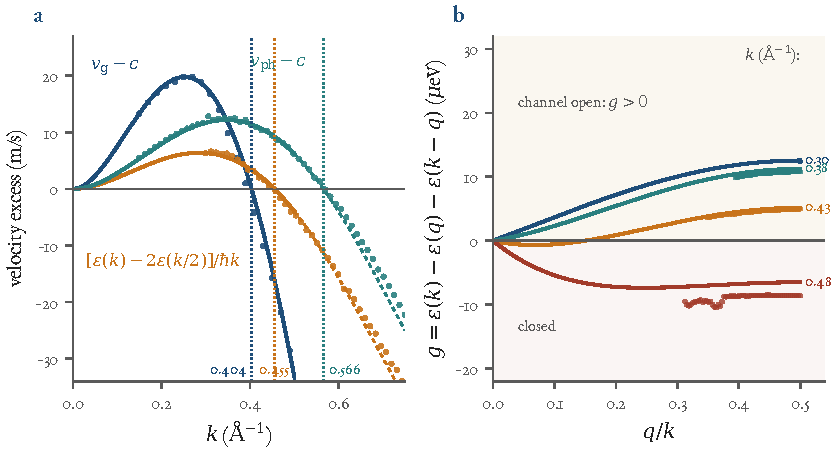
\includegraphics[width=\linewidth]{figures/ch05_thresholds.pdf}
\caption[Where the three-phonon channel closes]{\textbf{Where the three-phonon channel closes.}
\textbf{a}, the three excess velocities of \cref{ch05:eq-vph,ch05:eq-vg,ch05:eq-split} computed from the quartic series (lines; dotted beyond its stated range) and directly from the table (dots; the group velocity is a local linear fit over $\pm0.07\ \cfiveAng^{-1}$).
The zero crossings, in $\cfiveAng^{-1}$, are $\cfiveV{kGroup}$ ($v_{\rm g}=c$, soft emission), $\cfiveV{kSym}$ (symmetric split) and $\cfiveV{kPhase}$ ($v_{\rm ph}=c$).
\textbf{b}, the energy balance $g=\varepsilon(k)-\varepsilon(q)-\varepsilon(k-q)$ of a collinear decay $k\to q+(k-q)$ against $q/k$ for four wave numbers (lines: series; dots: table, where both $q$ and $k-q$ are at least $0.15\ \cfiveAng^{-1}$).
For $k=0.43\ \cfiveAng^{-1}$, between the first and the second threshold, the channel is closed at the soft end and open for near-symmetric splits.
Script: \texttt{figures/ch05\_thresholds.py}.}\label{ch05:fig-thresholds}
\end{figure}

\Cref{ch05:fig-thresholds} shows them, and shows the table agreeing.
Computed straight from the table, without the series, the symmetric split changes sign at $k=\cfiveV{kSymTable}\ \cfiveAng^{-1}$, against $\cfiveV{kSym}$ from the series; the maximum of the excess is $\cfiveV{symMax}$ micro-electronvolts at $\cfiveV{symMaxK}\ \cfiveAng^{-1}$, about three per cent of the energy $\varepsilon(k)$ there, and the series reproduces the table to $\cfiveV{seriesDevMax}$ micro-electronvolts at most for $0.25\le k\le0.5\ \cfiveAng^{-1}$.
This agreement is a consistency check and not an independent confirmation: the coefficients of the series were fitted by the authors to the very curve that the table tabulates.
What it does confirm is the kinematics: the soft end of the channel shuts first, near $\cfiveV{kGroup}\ \cfiveAng^{-1}$, then the symmetric split, and the two should not be mistaken for the sound-line crossing at $\cfiveV{kPhase}\ \cfiveAng^{-1}$, which closes nothing.

The calibration remark of \cref{ch05:sec-curve} pays off here, with a distinction.
The symmetric-split threshold is the zero of a function that is homogeneous of degree one in the energy scale, so it does not move at all if the roton-gap calibration is revised.
The other two compare the curve with the sound speed measured by ultrasonics, and are invariant only if that speed were rescaled with the curve; for a proportional change of the energy scale by the $\cfiveV{relSys}$ that the paper quotes as the relative systematic uncertainty, they move by at most $\cfiveV{shiftG}$ ($k_{\rm g}$) and $\cfiveV{shiftP}\ \cfiveAng^{-1}$ ($k_{\rm ph}$).

\subsection{Two rotons and the plateau}
There is a third kind of decay, with the same logic and a different threshold.
Above the roton the curve flattens into the shoulder that the authors, following the literature, call Pitaevskii's plateau, the energy at which one excitation can decay into two rotons \cite{Godfrin2021,GodfrinKrotscheck2022}.
Two rotons of wave number $k_{\rm R}$ carry a total momentum between $0$ (anti-parallel) and $2k_{\rm R}$ (parallel), so the plateau, which is the locus of the decay, cannot extend beyond $2k_{\rm R}$ in the collinear configuration and can in principle extend down to zero wave number through non-collinear ones, as the review explains \cite{GodfrinKrotscheck2022}.
The geometric core of this is the triangle inequality, and it is a theorem for any inner-product space: \Lthm{HeliumKinematics}{two_roton_momentum_le}, with the extremes attained by \Lthm{HeliumKinematics}{two_roton_parallel} and \Lthm{HeliumKinematics}{two_roton_antiparallel}.
The plateau is not used quantitatively in this book, and nothing is claimed about the data there.

%% ====================================================================================================================
\section{Bogoliubov's phonon, and what it cannot do}\label{ch05:sec-bogoliubov}

\subsection{A phonon that turns into a particle}
There is one quantum fluid in which the whole dispersion relation can be derived on a page, and it is the one the solver simulates.
Take the Gross--Pitaevskii equation with $\hbar=m=1$,
\begin{equation}\label{ch05:eq-gpe}
 \mathrm i\,\partial_t\psi=-\tfrac12\nabla^2\psi+g|\psi|^2\psi ,
\end{equation}
and the uniform solution $\psi_0=\sqrt{n}\,\mathrm e^{-\mathrm i\mu t}$ with $\mu=gn$.
Write $\psi=\mathrm e^{-\mathrm i\mu t}(\sqrt n+\delta)$ and keep terms linear in $\delta$: $\mathrm i\,\partial_t\delta=-\tfrac12\nabla^2\delta+gn(\delta+\delta^*)$.
A plane-wave pair $\delta=u\,\mathrm e^{\mathrm i(kx-\omega t)}+v^*\mathrm e^{-\mathrm i(kx-\omega t)}$ turns this into a two-by-two eigenvalue problem whose determinant gives
\begin{equation}\label{ch05:eq-bog}
 \omega^2=\tfrac12k^2\bigl(\tfrac12k^2+2gn\bigr)\qquad\Longleftrightarrow\qquad
 \varepsilon(k)=\sqrt{c^2\hbar^2k^2+\bigl(\hbar^2k^2/2m\bigr)^2},\quad c^2=\frac{gn}{m},
\end{equation}
the formula Bogoliubov found in 1947 \cite{Bogoliubov1947} (see also \cite{Dalfovo1999,PitaevskiiStringari2016}).
It is a phonon, $\varepsilon\simeq\hbar ck$, below the wave number
\begin{equation}
 k_\ast=\frac{2mc}{\hbar},
\end{equation}
and a free particle, $\varepsilon\simeq\hbar^2k^2/2m$, above it; the wave number $k_\ast$ is the inverse of the healing length of the condensate up to a numerical factor (with $\xi=\hbar/mc$, the convention of the solver, $k_\ast\xi=2$).
The phonon \emph{turns into a particle} as $k$ increases, and the whole curve depends on the single wave number $k_\ast$: for $c,m,k>0$,
\begin{equation}\label{ch05:eq-universal}
 \frac{\varepsilon(k)}{ck}=\sqrt{1+(k/k_\ast)^2}
\end{equation}
(\Lthm{BogoliubovDispersion}{phase_velocity_universal}).
Everything that follows about Bogoliubov's curve is a statement about this one function.
These excitations are waves of density and of phase in a single-valued $\psi$: the velocity they carry, $\hbar\nabla S/m$ for $\psi=\sqrt\rho\,\mathrm e^{\mathrm iS}$, is the gradient of a single-valued phase, so it is irrotational and carries no circulation.
They are the first of the two kinds of excitation of the same field distinguished in \cref{ch03}; the second kind, the vortices, is not in the linearised equation at all.

\subsection{What is proved about it}
Several properties of \cref{ch05:eq-bog} are used below, and each is a theorem in the new Lean module written for this chapter, the file \texttt{Ch05\_\allowbreak BogoliubovDispersion}, whose namespace is \texttt{QuantumFluids.\allowbreak BogoliubovDispersion}; the module is new and is not part of the library \texttt{QuantumFluids}.
Its definitions are the Bogoliubov energy and the curvature coefficient, and its first theorem is the dictionary between the solver's parameters and the formula,
$\varepsilon^2=\tfrac12k^2(\tfrac12k^2+2gn)$ when $c^2=gn$ and $m=1$ (\Lthm{BogoliubovDispersion}{bogEps_sq_gp}), which is the expression the solver's known answer K5 is tested against in \cref{ch05:sec-solver}.
The module proves:
\begin{itemize}
 \item $\varepsilon$ is strictly increasing on $[0,\infty)$ (\Lthm{BogoliubovDispersion}{bogEps_strictMonoOn}): there is no maxon, no roton, no stationary point at all;
 \item $\varepsilon(k_1)+\varepsilon(k_2)<\varepsilon(k_1+k_2)$ for all $k_1,k_2>0$ (\Lthm{BogoliubovDispersion}{bogEps_superadditive}): the collinear decay of a phonon into two is open at \emph{every} wave number, not only below a critical one --- the spectrum is anomalous throughout, in the sense of \cref{ch05:sec-decays}, which is the kinematic precondition of what the literature calls Beliaev damping (its rate is not computed here);
 \item $\varepsilon(k)-ck$ is strictly increasing (\Lthm{BogoliubovDispersion}{bogEps_sub_sound_strictMonoOn}): the energy of an excitation outruns the sound line at every wave number, the derivative-free form of the statement that the group velocity exceeds $c$;
 \item the low-$k$ expansion has the curvature coefficient $\alpha_2=1/(8m^2c^2)$, with the explicit error band below;
 \item the Landau velocity of the spectrum is $c$, exactly.
\end{itemize}
The last two are worth displaying.
The first is the quantitative form of the expansion, a two-sided bound whose proof is the elementary inequality $\sqrt{1+2t}\le1+t$ and its refinement $\sqrt{1+2t}\ge1+t-t^2/2$:

\begin{leanbox}[title={Lean 4 \enspace BogoliubovDispersion (new for this book)}]{BogoliubovDispersion (new)}
\begin{lstlisting}[style=lean]
noncomputable def bogEps (c m k : ℝ) : ℝ := Real.sqrt (c ^ 2 * k ^ 2 + (k ^ 2 / (2 * m)) ^ 2)

noncomputable def alpha2 (c m : ℝ) : ℝ := 1 / (8 * m ^ 2 * c ^ 2)

theorem abs_bogEps_sub_phononDisp_le {c m k : ℝ} (hc : 0 < c) (hm : 0 < m) (hk : 0 ≤ k) :
    |bogEps c m k - phononDisp c (alpha2 c m) k| ≤ c * (alpha2 c m) ^ 2 * k ^ 5 / 2

theorem landau_velocity_eq {c m : ℝ} (hc : 0 < c) (hm : 0 < m) :
    IsGLB ((fun k => bogEps c m k / k) '' Set.Ioi 0) c
\end{lstlisting}
\end{leanbox}

\noindent Here \texttt{phononDisp} is the definition of the library repeated verbatim in the new file, so that the module can be compiled alone.
In words: the Bogoliubov energy differs from $ck(1+\alpha_2k^2)$ by at most $c\alpha_2^2k^5/2$, so the curvature coefficient of the phonon branch is $1/(8m^2c^2)>0$ and the error of the quadratic correction is of order $k^5$ (\Lthm{BogoliubovDispersion}{alpha2_limit} states the limit); and the infimum of the phase velocity $\varepsilon/k$ over $k>0$ is exactly $c$ and is not attained, because $\varepsilon/k=\sqrt{c^2+k^2/4m^2}>c$ at every $k>0$ (\Lthm{BogoliubovDispersion}{sound_lt_phase_velocity}).
By Landau's criterion the critical velocity of this superfluid is therefore its sound speed and nothing less: no excitation of the Bogoliubov spectrum is cheaper per unit momentum than a phonon.
The proof of the upper half of the band is short enough to show, in the form in which it was compiled; the auxiliary identity \texttt{eps\_arg} that it uses ($c^2k^2+(k^2/2m)^2=(ck)^2(1+2\alpha_2k^2)$, by \texttt{field\_simp; ring}) is not shown (proof abridged):

\begin{leanbox}[title={Lean 4 \enspace BogoliubovDispersion (new for this book)}]{BogoliubovDispersion (new)}
\begin{lstlisting}[style=lean]
theorem bogEps_le_phononDisp {c m k : ℝ} (hc : 0 < c) (hm : 0 < m) (hk : 0 ≤ k) :
    bogEps c m k ≤ phononDisp c (alpha2 c m) k := by
  have ha : 0 < alpha2 c m := by unfold alpha2; positivity
  unfold bogEps phononDisp
  rw [Real.sqrt_le_iff]
  refine ⟨by positivity, ?_⟩
  rw [eps_arg hc hm]                       -- (ck)^2 (1 + 2t), t = alpha2 k^2
  have : (c * k) ^ 2 * (1 + 2 * (alpha2 c m * k ^ 2)) ≤ (c * k) ^ 2 * (1 + alpha2 c m * k ^ 2) ^ 2 := by
    apply mul_le_mul_of_nonneg_left _ (sq_nonneg _)
    nlinarith [sq_nonneg (alpha2 c m * k ^ 2)]   -- 1+2t <= (1+t)^2
  calc _ ≤ _ := this
    _ = _ := by ring
\end{lstlisting}
\end{leanbox}

\noindent The lower half is the same argument with $(1+t-t^2/2)^2\le1+2t$, valid when $1+t-t^2/2\ge0$; when that quantity is negative the lower bound is itself negative and holds trivially, because $\varepsilon\ge0$.
All of it was compiled with Lean~4 and Mathlib on the machine that ran the solver, with no \texttt{sorry} and only the three standard axioms.

\subsection{Against helium: how far is the real curve from the weak-coupling one?}
Bogoliubov's derivation assumes a dilute gas whose interaction can be replaced by one coupling constant.
Liquid helium is neither.
Still the \emph{shape} of \cref{ch05:eq-bog} can be compared with the measured curve with no free parameter, because the formula has only two inputs, the mass and the sound speed, and both are known: the bare mass of the $^4$He atom and $c=\cfiveV{c}\ \mathrm{m\,s^{-1}}$.
With them the wave number of the problem is $k_\ast=2mc/\hbar=\cfiveV{kstar}\ \cfiveAng^{-1}$, which is \emph{inside} the measured range, and the curvature coefficient of the phonon branch is $\alpha_2^{\rm Bog}=1/(2k_\ast^2)=\cfiveV{alphaBog}\ \cfiveAng^2$, against the measured $1.55\ \cfiveAng^2$: the real curve bends away from the sound line \cfiveV{alphaRatio} times faster.
\Cref{ch05:fig-curve}b,c show the comparison; the Bogoliubov phase velocity climbs without limit while the measured one turns over at $k\approx\cfiveV{phaseMaxK}\ \cfiveAng^{-1}$ and falls to a quarter of $c$.

The two-sided reading is the point of this book's rule about analogies.
The comparison measures \emph{how far helium is from the hypotheses that Bogoliubov's formula needs}; it does not test the formula, which is a theorem about the Gross--Pitaevskii equation, and it does not say that a gas with those parameters would behave like helium.
A property that the roton depends on is not a property of the Gross--Pitaevskii equation with a contact interaction: a monotonically increasing $\varepsilon$ has no minimum, whatever the value of $g$.
The roton needs structure on the scale of the interatomic distance.
Feynman's account is that the energy of the excitation is, at best, $\hbar^2k^2/2mS(k)$, with $S(k)$ the static structure factor, and that this is an \emph{upper bound} to the true excitation energy \cite{Feynman1954,FeynmanCohen1956}; the minimum of $\varepsilon$ sits where $S(k)$ has its first peak, the signature of the short-range order of the liquid.
In the weak-coupling theory $S(k)=(\hbar^2k^2/2m)/\varepsilon(k)$ and the bound is saturated; in helium it is not, and the paper itself remarks that the Bijl--Feynman spectrum is ``clearly very far from the experimental result'' \cite{Godfrin2021}.

A different mechanism produces a roton minimum in a Bose gas, and the difference is the lesson of this section.
Give the atoms a non-local interaction whose Fourier transform $V(k)$ becomes negative in a window, as for dipolar atoms, and the Bogoliubov spectrum becomes $\omega^2=\epsilon_k(\epsilon_k+2nV(k))$ with $\epsilon_k=\hbar^2k^2/2m$: it can have a roton minimum, and such rotons have been seen in a dipolar quantum gas \cite{Santos2003,Chomaz2018}.
That is a mean-field roton produced by the sign of an interaction in $k$-space; the helium roton is the signature of short-range order.
The two share a name and a shape, and the properties that depend on the mechanism --- what the roton mass is, how it responds to pressure, what it does at the liquid--solid transition --- are not transferable from one to the other without checking (Exercise~3).


%% ====================================================================================================================
\section{The solver as a spectrometer}\label{ch05:sec-solver}

The projected Gross--Pitaevskii equation is the one quantum fluid of this book whose dispersion relation is known in closed form, and that makes it a test bench: if the excitations of the simulated field do not obey \cref{ch05:eq-bog}, the instrument is wrong.
The instrument is \texttt{qf-pgpe}, the Rust engine of rusty-SUNDIALS that \cref{ch02} describes.
It integrates $\mathrm i\,\partial_t\psi=P[-\tfrac12\nabla^2\psi+g|\psi|^2\psi]$ on a doubly periodic box with an integrating-factor fourth-order Runge--Kutta step (the linear part exact, the cubic part by RK4) and a sharp circular cutoff $P$ at $k_{\rm cut}=k_{\max}/2$, which is the condition under which the cubic term does not alias into the retained modes.
The crate's own documentation records agreement with the numpy engine of the programme to $10^{-10}$ over twenty time units \cite{Callens2026sw}.
Units are $\hbar=m=n_0=1$ and $g=1$, so that $c=1$, $\xi=\hbar/mc=1$ and $k_\ast=2$.
The box is $L=64\,\xi$ on a $128\times128$ grid, which retains \cfiveV{nmodesRetained} wave vectors with $|k|\le\pi/\xi$.

\subsection{Exciting every mode at once}
A time-of-flight spectrometer covers hundreds of scattering angles at once, and the simulation can do the same.
Start from the uniform condensate $\psi=1$ and add a weak random complex amplitude, of size $\eta=10^{-6}$, to \emph{every} retained mode; evolve for $T=\cfiveV{Tmain}$; every $0.4$ time units record the amplitude $c_k(t)$ of every mode.
In the linear regime each mode then oscillates as a superposition of the two normal modes of the pair $\pm k$, so that, with the proper frame (next paragraph),
\begin{equation}\label{ch05:eq-twofreq}
 s_k(t)=\alpha_k\,\mathrm e^{-\mathrm i\omega_kt}+\beta_k\,\mathrm e^{+\mathrm i\omega_kt},
\end{equation}
two complex amplitudes and one frequency per mode.
For each mode the frequency is the value of $\omega$ that minimises the residual of the best linear fit of the two amplitudes; the residual is evaluated in closed form, and a golden-section search, started from a one-step linear-prediction estimate, finds the minimum in \cfiveV{nGolden} evaluations.
The half-records give a model-free error proxy: the two halves of the record are fitted separately and the difference is reported.
One run yields \cfiveV{nModesMain} measurements of the dispersion relation.

\subsection{The frame lesson}
The record is kept in the \emph{condensate frame}, $s_k=c_k\,c_0^\ast/|c_0|$, where $c_0$ is the amplitude of the $k=0$ mode, and the reason is an episode that the programme recorded as a failure.
In its pre-registered list of known answers for the engine, the Bogoliubov test (called K5) failed at the first attempt, by factors of $5$, $2.5$ and $1.2$ in the frequency, before any physics was run \cite{Callens2026prereg}.
The cause was not the engine.
The equation has no chemical potential in it, so the condensate rotates in the laboratory frame as $\mathrm e^{-\mathrm i\mu t}$ with $\mu=gn_0$, and every mode amplitude inherits that phase: the measured frequencies were $\mu\pm\omega$.
The record of this run shows it directly.
For the mode $(16,0)$, $k=\cfiveV{labK}$, the Bogoliubov frequency is $\omega=\cfiveV{labOmega}$, and the laboratory-frame record has its two spectral peaks at $\cfiveV{labPeakA}$ and $+\cfiveV{labPeakB}$, which are $-(\mu+\omega)=\cfiveV{labExpA}$ and $-\mu+\omega=+\cfiveV{labExpB}$ to within the $10^{-3}$ resolution of the peak position.
Reading the larger peak as the excitation frequency gives about $3$ where the answer is $2$; reading the smaller gives about $1$.
Dividing by the condensate's phase fixed the test.
The same logic holds for the experiment: a neutron's energy loss $E_i-E_f$ is measured against the ground state of the liquid, and the chemical potential of the liquid never appears.
A frequency is a statement about a frame.

\begin{rustbox}{the broadband pulse and the condensate frame}
\begin{lstlisting}[style=py,basicstyle=\ttfamily\footnotesize]
import numpy as np, qf_pgpe
eng = qf_pgpe.Pgpe(N, L, g, dt, 0.5)             # n, L, g, dt, k_cut/k_max

def initial_pulse(eng, N, eta, seed):                 # (docstring removed)
    rng = np.random.default_rng(seed)
    mask = mode_set(eng, N)
    c = np.array(eng.uniform(), dtype=complex)
    xi = (rng.normal(size=(N, N)) + 1j * rng.normal(size=(N, N))) / np.sqrt(2.0)
    add = eta * N ** 2 * xi * mask
    add[0, 0] = 0.0
    return c + add, mask

def record_condensate_frame(run_step, c0, mask, n_samples, N, keep_lab=None):
    c = c0                                            # (docstring removed)
    nm = int(mask.sum())
    out = np.empty((n_samples, nm), dtype=np.complex128)
    lab = np.empty(n_samples, dtype=np.complex128) if keep_lab is not None else None
    for j in range(n_samples):
        if j > 0:
            c = run_step(c)                       # eng.run(c, 0.4): 20 steps
        c = np.asarray(c)
        ph = np.conj(c[0, 0]) / abs(c[0, 0])  # condensate frame: remove exp(-i mu t)
        out[j] = c[mask] * ph / N ** 2
        if lab is not None:
            lab[j] = c[keep_lab] / N ** 2
    return out, lab
\end{lstlisting}
\end{rustbox}

The code is the code that was run (\cfivepath{figures/ch05_common.py}; the main run is \cfivepath{figures/ch05_dispersion_run.py}).
The main run, $15\,000$ steps of a $128^2$ grid, took \cfiveV{secRun} seconds of wall time, plus \cfiveV{secFit} seconds of fitting, on the shared eight-core machine of this project while its load average was between ten and thirty-six; the figure is indicative of the order of magnitude and not a benchmark.

\subsection{What the measurement shows}
\begin{figure}[tp]
\centering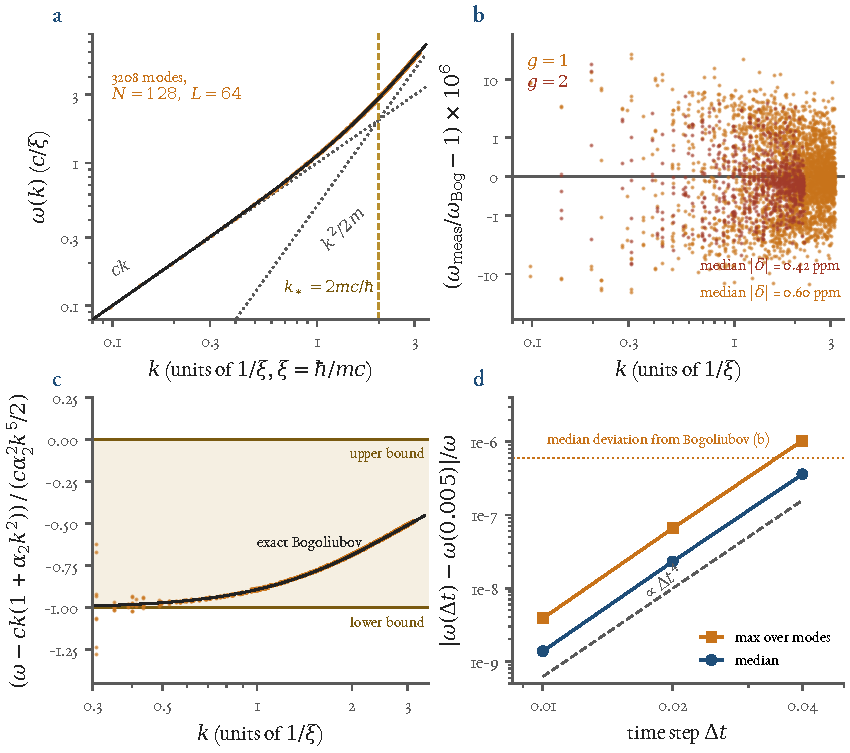
\includegraphics[width=\linewidth]{figures/ch05_solver.pdf}
\caption[The solver measures Bogoliubov's dispersion relation]{\textbf{The solver measures Bogoliubov's dispersion relation.}
\textbf{a}, the frequencies of all \cfiveV{nModesMain} modes of the $128^2$ run (orange) on the Bogoliubov curve (black) between its two asymptotes (dotted).
\textbf{b}, the relative deviation of every mode from $\omega_{\rm Bog}$, in parts per million, for $g=1$ and for a second run with $g=2$ ($c=\sqrt2$; the wave number is in units of $1/\xi=mc/\hbar$).
\textbf{c}, the band proved in Lean: the quantity $(\omega-ck(1+\alpha_2k^2))/(c\alpha_2^2k^5/2)$ lies in $[-1,0]$ for the Bogoliubov spectrum, and the measured points follow the exact curve (black) from the lower edge, which is asymptotically sharp as $k\to0$.
Below $k\approx0.5$ the noise of the fit, magnified by the $k^{-5}$ of the normalisation, takes some points out of the band; the band is a theorem about the formula, the points are measurements.
\textbf{d}, the time-step ladder: differences between the frequencies obtained with $\Delta t=0.04$, $0.02$, $0.01$ and those of the same pulse with $\Delta t=0.005$; they fall by a factor $\cfiveV{ratioA}$ and then $\cfiveV{ratioB}$ per halving, the fourth-order law of the scheme.
Script: \texttt{figures/ch05\_dispersion\_run.py} (data), \texttt{figures/ch05\_solver\_fig.py} (figure).}\label{ch05:fig-solver}
\end{figure}

\Cref{ch05:fig-solver}a shows the result: all \cfiveV{nModesMain} frequencies, over almost a decade and a half in $k$, lie on Bogoliubov's curve, bending from the sound line to the free-particle parabola across $k_\ast$.
The deviations (\cref{ch05:fig-solver}b) have a median of $\cfiveV{medMain}$ parts per million, $99$ per cent of the modes are within $\cfiveV{p99Main}$ ppm and the worst is $\cfiveV{maxMain}$ ppm.
The error is not uniform in $k$: the median is $\cfiveV{medLowK}$ ppm below $k=0.4$ and $\cfiveV{medHighK}$ ppm above $k=2.5$, because the slowest modes complete only a few periods in the record; the half-record difference, which is blind to the model, has a median of $\cfiveV{medSplit}$ ppm and says the same.
So this is a statement about the fit as much as about the engine, and it is a good one: the engine's frequencies equal the closed form to a few parts in $10^7$.

Three further checks sit in the same figure.
The second run, with $g=2$, gives a median of $\cfiveV{medG2}$ ppm over $\cfiveV{nModesG2}$ modes: the dictionary $c^2=gn_0$ of \Lthm{BogoliubovDispersion}{bogEps_sq_gp} is right.
The Lean theorem \Lthm{BogoliubovDispersion}{abs_bogEps_sub_phononDisp_le} meets data in the band of \cref{ch05:fig-solver}c: for the $\cfiveV{nBand}$ modes with $k\ge0.5$ all of the points lie inside $[-1,0]$, between $\cfiveV{zMin}$ and $\cfiveV{zMax}$, and the largest distance from the exact curve is $\cfiveV{zDev}$ in these units.
The ladder of \cref{ch05:fig-solver}d is the integrator's own order: the median difference to the finest run is $\cfiveV{ladA}$, $\cfiveV{ladB}$ and $\cfiveV{ladC}$ for $\Delta t=0.04$, $0.02$, $0.01$, a drop of $\cfiveV{ratioA}$ and $\cfiveV{ratioB}$ per halving.
At the step used for the main run, $\Delta t=0.02$, the time-stepping error is therefore a factor $\cfiveV{ladVsFit}$ smaller than the fit's own scatter.

\subsection{One function of one variable}
\begin{figure}[tp]
\centering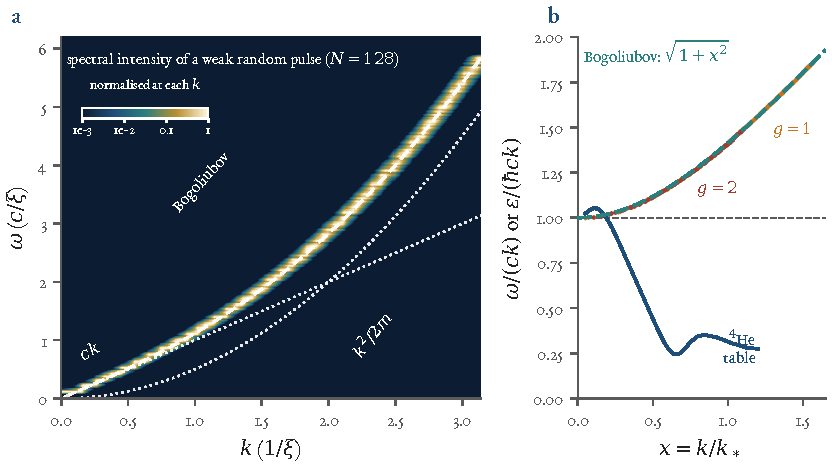
\includegraphics[width=\linewidth]{figures/ch05_universal.pdf}
\caption[A spectrometer map of the simulated fluid, and the universal curve]{\textbf{A spectrometer map of the simulated fluid, and the universal curve.}
\textbf{a}, the power spectrum of the record of every mode, folded onto positive frequency, smeared in $k$ with a Gaussian of width $0.03/\xi$ (a display resolution, like the finite angular resolution of an instrument), and normalised at each $k$.
A bright ridge follows the Bogoliubov curve (white, dashed) from the sound line to the free-particle parabola (dotted).
The intensity along the ridge is set by the random pulse and has no physical meaning; only the position of the ridge does.
\textbf{b}, the phase velocity in units of $c$ against $x=k/k_\ast$, $k_\ast=2mc/\hbar$: the $g=1$ run (orange) and the $g=2$ run (red) fall on the single curve $\sqrt{1+x^2}$ (teal) of \cref{ch05:eq-universal}, to within $\cfiveV{collapseA}$ and $\cfiveV{collapseB}$; the measured curve of $^4$He (blue, with the bare atomic mass and $c=238.3$ m/s in $k_\ast$) leaves it at $x\approx0.1$ and has no part in common with it beyond.
Script: \texttt{figures/ch05\_solver\_fig.py}.}\label{ch05:fig-universal}
\end{figure}

Equation~\eqref{ch05:eq-universal} says that the whole curve is a function of one variable, and the two runs test it.
In the coordinates $x=k/k_\ast$ and $y=\omega/(ck)$ the $g=1$ and the $g=2$ runs, whose sound speeds differ by $\sqrt2$ and whose cutoffs sit at different $x$, collapse on $\sqrt{1+x^2}$ to within $\cfiveV{collapseA}$ and $\cfiveV{collapseB}$ (\cref{ch05:fig-universal}b).
Helium, in the same coordinates with the bare atomic mass, does not: it leaves the universal curve at $x\approx0.1$, rises to $\cfiveV{phaseMaxRatio}$ and falls to $\cfiveV{rotonYat}$ at the roton.
The two curves have the same two inputs and nothing else in common.

\Cref{ch05:fig-universal}a is the same data seen as an experimentalist sees $S(Q,\omega)$: a map in the $(k,\omega)$ plane, with a bright line where the excitations are.
It is, if one likes, a numerical neutron-scattering experiment.
It shows no maxon and no roton, only a ridge that never turns over, and the point of the figure is that contrast: the line a neutron spectrometer draws for helium (\cref{ch05:fig-curve}a) has structure that a contact-interaction Gross--Pitaevskii field cannot produce.
Two caveats keep the analogy honest.
The intensity along the ridge is an artefact of our random pulse; the physical weight of the single-excitation peak is the static structure factor $S(k)=(\hbar^2k^2/2m)/\varepsilon(k)$ of Bogoliubov's theory, and a classical field at zero temperature has no way to produce it.
And the lines of the map are as sharp as the window allows, because the field is integrated for three hundred time units without damping; what limits the width of the excitation peaks in real helium --- the decay channels of \cref{ch05:sec-decays} --- is not computed here.

\subsection{Waves in space: the group velocity}
The frequency of one wave number is one way to see the dispersion; a wave packet is another, and it measures a different quantity, the group velocity.
\begin{figure}[tp]
\centering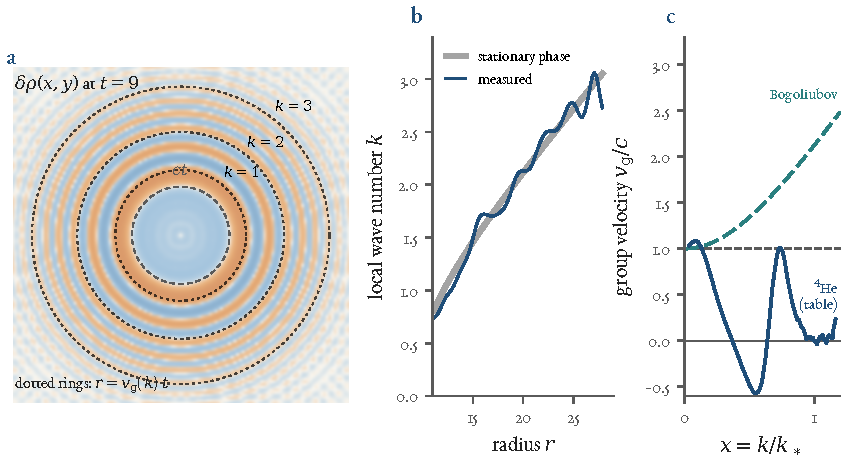
\includegraphics[width=\linewidth]{figures/ch05_rings.pdf}
\caption[A dispersive ring wave]{\textbf{A dispersive ring wave.}
\textbf{a}, the density deviation $\delta\rho$ (symmetric logarithmic colour scale) at $t=9$ after a Gaussian density bump of width $0.6\,\xi$ and height $0.02$ at the centre of the box (zero initial velocity; $128^2$ grid, $L=64\,\xi$, bicubic interpolation for display).
The ring at $r=ct$ is the sound front; outside it the ripples are the short waves that run ahead, each wave number $k$ at the radius $v_{\rm g}(k)\,t$ (dotted circles for $k=1,2,3$).
\textbf{b}, the local wave number of the azimuthally averaged profile (blue; phase of the analytic signal of $\sqrt r\,\delta\rho$) against the stationary-phase prediction $v_{\rm g}(k_s)=r/t$ (grey).
\textbf{c}, the group velocity in units of $c$ against $x=k/k_\ast$: Bogoliubov (teal, dashed) rises monotonically to $\cfiveV{vgKcut}\,c$ at the cutoff; for $^4$He (blue, local linear fit to the table) it reaches only $\cfiveV{vgMax}\,c$ near $\cfiveV{vgMaxK}\ \cfiveAng^{-1}$, vanishes at the maxon ($\cfiveV{vgZeroK}\ \cfiveAng^{-1}$), turns negative ($\cfiveV{vgMin}\,c$ at $\cfiveV{vgMinK}\ \cfiveAng^{-1}$) and returns to zero at the roton.
Script: \texttt{figures/ch05\_rings.py}.}\label{ch05:fig-rings}
\end{figure}
A localised density pulse contains all wave numbers.
Each travels at its own group velocity $v_{\rm g}=\mathrm d\omega/\mathrm dk=(k+k^3/2)/\omega$ (units $c=m=\hbar=1$), so that the stationary-phase argument puts the wave number $k$ at the radius $r=v_{\rm g}(k)\,t$: a snapshot of the density is a map of the dispersion relation read through its derivative.
Since $\varepsilon(k)-ck$ is increasing (\Lthm{BogoliubovDispersion}{bogEps_sub_sound_strictMonoOn}), the mean group velocity between any two wave numbers exceeds $c$, and the ripples run ahead of the front.
\Cref{ch05:fig-rings} shows it.
The local wave number of the ripples, measured in the range $r=\cfiveV{ringRmin}$ to $\cfiveV{ringRmax}\,\xi$ (wave numbers $\cfiveV{ringKmin}$ to $\cfiveV{ringKmax}/\xi$), follows the stationary-phase prediction with a median relative deviation of $\cfiveV{ringMed}$ per cent (largest: $\cfiveV{ringMax}$ per cent at the edges of the window, where the phase of the analytic signal is least reliable).
No fit and no free parameter enters: the dispersion relation has been read off a single snapshot, and it is the same one that was read off $\cfiveV{nModesMain}$ time series.

Panel c is the comparison with the helium of \cref{ch05:sec-curve}, in the universal coordinate $x$.
The group velocity of Bogoliubov's fluid exceeds $c$ at every wave number and grows without bound ($\cfiveV{vgKcut}\,c$ at the cutoff of the simulation).
The group velocity of helium, computed from the table by a local linear fit, rises above $c$ by $\cfiveV{vgMaxPct}$ per cent near $\cfiveV{vgMaxK}\ \cfiveAng^{-1}$ and returns to $c$ at $\cfiveV{vgCrossK}\ \cfiveAng^{-1}$ (the series of \cref{ch05:sec-decays} gives $\cfiveV{kGroup}$); it vanishes at the maxon, is negative between maxon and roton --- excitations whose energy increases while their momentum decreases --- and vanishes again at the roton.
A pulse launched in helium would therefore send ahead of the sound front only the waves with $k$ below about $\cfiveV{vgCrossK}\ \cfiveAng^{-1}$, and the waves between the maxon ($\cfiveV{vgZeroK}\ \cfiveAng^{-1}$) and the roton would travel backwards.
Both statements are consequences of the shape of the table, and neither has been seen in a simulation here, since the engine cannot produce this curve.

\subsection{A referee: CVODE}
The engine is a fixed-step scheme of known order (\cref{ch05:fig-solver}d); an integrator of a different kind is a useful second opinion.
The projected equation is an ordinary differential system for $2n_{\rm modes}$ real numbers, and CVODE, the variable-order solver of rusty-SUNDIALS, integrates it through its Python module \texttt{rusty\_sundials} with the right-hand side supplied from Python.
The interface returns the end state only, so a time series is built by chaining one call per sample interval; the Adams method is the sensible choice for a non-stiff problem.
\begin{rustbox}{the same trajectory under CVODE}
\begin{lstlisting}[style=py,basicstyle=\ttfamily\footnotesize]
# abridged from figures/ch05_cvode.py
from rusty_sundials import CvodeSolver
scale = float(N ** 2)

def rhs(_t, y):                          # dc/dt of the projected GPE; y = (Re c, Im c) / N^2
    c = py.unpack(np.asarray(y) * scale)  # py: numpy engine, same equation, same modes
    return (py.pack(py.rhs(c)) / scale).tolist()

solver = CvodeSolver("adams", rtol, atol, 10_000_000)
y = (py.pack(c0) / scale).tolist()
for j in range(1, ns):
    _, y = solver.solve(rhs, (j - 1) * dts, y, j * dts)   # one call per sample interval
\end{lstlisting}
\end{rustbox}
This cross-check has a history that belongs to the record.
The software paper of the engine makes the same comparison, the engine against a CVODE reference on a box of $16\times16$ points with $49$ modes, and reports that it depends on a fix of the library, ``the Adams order was stuck at one'': without the fix the solver collapses its step on this oscillatory Hamiltonian problem and fails after about $10^6$ right-hand-side evaluations \cite{Callens2026sw}.
The module installed in the project's virtual environment predates the fix (it was installed on \cfiveV{cvOldDate}), and \cref{ch05:tab-cvode-builds} shows the difference from the outside: on a box of $\cfiveV{cvSmallN}\times\cfiveV{cvSmallN}$ points the older build needs $\cfiveV{cvRatio4}$, $\cfiveV{cvRatio6}$ and $\cfiveV{cvRatio8}$ times as many right-hand-side evaluations as the current one at tolerances $10^{-4}$, $10^{-6}$ and $10^{-8}$.
At the same tolerance it is also less accurate (at $10^{-6}$ its frequencies differ from the engine's by $\cfiveV{cvOldErr6}$, those of the current build by $\cfiveV{cvNewErr6}$).
Its cost grows roughly as the inverse square root of the tolerance (by factors of $\cfiveV{cvGrowOldA}$ and $\cfiveV{cvGrowOldB}$ for each hundredfold tightening, where an exact square-root law gives ten) and its error falls by about $\cfiveV{cvOldFallA}$ and $\cfiveV{cvOldFallB}$ over the same steps, which is how a first-order method behaves when the step is set by an error that is quadratic in the step.
The first attempt at this section was run on the older build and was abandoned for that reason; everything below uses the current build.
% generated by ch05_numbers.py from ch05_cvode_new.json / ch05_cvode_old.json
\begin{table}[t]\centering\small
\begin{tabular}{rrrrr}\toprule
tolerance (rtol) & \multicolumn{2}{c}{older build} & \multicolumn{2}{c}{current build}\\
 & right-hand sides & $\max|\Delta\omega|/\omega$ & right-hand sides & $\max|\Delta\omega|/\omega$ \\\midrule
\ensuremath{10^{-4}} & 1\,361 & \ensuremath{1.9\times10^{-2}} & 599 & \ensuremath{3.8\times10^{-4}} \\
\ensuremath{10^{-6}} & 9\,730 & \ensuremath{1.7\times10^{-3}} & 718 & \ensuremath{1.7\times10^{-5}} \\
\ensuremath{10^{-8}} & 91\,519 & \ensuremath{1.7\times10^{-4}} & 992 & \ensuremath{3.5\times10^{-7}} \\
\bottomrule\end{tabular}
\caption{\textbf{The same experiment on two builds of the Python module.} A box of $8^2$ grid points ($13$ modes, $26$ unknowns), $T=4$, the same pulse. The older build is the module of the project's virtual environment (installed on \cfiveV{cvOldDate}); the current one was built from the rusty-SUNDIALS tree (commit 5db8041) that contains the fix of the Adams order.}\label{ch05:tab-cvode-builds}
\end{table}

\begin{table}[t]\centering\small
\begin{tabular}{rrrrr}\toprule
tolerance (rtol) & right-hand sides & wall (s) & $\max|\Delta\omega|/\omega$ & $\max|\Delta s|/|s|$ \\\midrule
\ensuremath{10^{-4}} & 6\,229 & 4.8 & \ensuremath{7.8\times10^{-4}} & \ensuremath{7.7\times10^{-2}} \\
\ensuremath{10^{-6}} & 6\,948 & 5.4 & \ensuremath{2.7\times10^{-5}} & \ensuremath{1.6\times10^{-3}} \\
\ensuremath{10^{-8}} & 8\,313 & 7.0 & \ensuremath{2.7\times10^{-7}} & \ensuremath{1.8\times10^{-5}} \\
\ensuremath{10^{-10}} & 10\,158 & 7.6 & \ensuremath{3.3\times10^{-9}} & \ensuremath{8.0\times10^{-7}} \\
\bottomrule\end{tabular}
\caption{\textbf{CVODE against the Rust engine.} The same random pulse ($\eta=10^{-4}$) on a box of \cfiveV{cvN}$^2$ grid points with \cfiveV{cvModes} retained modes ($\cfiveV{cvUnknowns}$ real unknowns), integrated to $T=\cfiveV{cvT}$ by CVODE's Adams method (atol $=10^{-3}\,$rtol) through the Python interface and by the engine ($\Delta t=0.01$ and a four times smaller step as reference).
Columns: right-hand-side evaluations, wall time on the shared machine, the largest relative difference between the frequencies read from the CVODE record and from the fine-step engine record, and the largest difference between the two mode records, relative to the rms amplitude of each mode.
The engine's own frequencies differ from its four-times-finer run by at most \cfiveV{cvRk4Dt}, and the engine took \cfiveV{cvRustSec} s for this record.
Both records go through the same fit; the frequencies of this short record, in which the modes complete between \cfiveV{cvPerMin} and \cfiveV{cvPerMax} periods, differ from Bogoliubov's formula by up to \cfiveV{cvBogMax}, which cancels in the difference between the two records.}\label{ch05:tab-cvode}
\end{table}

With the current build CVODE does what a referee should (\cref{ch05:tab-cvode}).
The box is that of the software paper's reference, $\cfiveV{cvN}\times\cfiveV{cvN}$ points with $\cfiveV{cvModes}$ modes, integrated here for $\cfiveV{cvT}$ time units.
As the tolerance is tightened from $10^{-4}$ to $10^{-10}$ the frequencies that CVODE gives approach those of the finest run of the engine, the difference falling from $\cfiveV{cvErr4}$ to $\cfiveV{cvErr10}$; the last two rows are below the $\cfiveV{cvRk4Dt}$ by which the engine at its production step differs from that finest run.
The finest run is not exact either: for a scheme of fourth order the error of the run with the four times smaller step is about $1/255$ of that difference, that is $\cfiveV{cvFineErr}$, which is of the order of the last difference, so the comparison cannot resolve more.
Two independent integrators, one of fixed step and fourth order and one of variable order and step, agree on the dispersion relation of the projected equation: the frequencies that the same fit reads from their records differ by $\cfiveV{cvBestErr}$ at most.
What the referee cannot do is scale.
Every right-hand-side evaluation is a call from CVODE into Python, where the numpy engine evaluates the equation and the state is converted to and from a list, and both the number of evaluations and the cost of each one grow with the box: for two time units at tolerance $10^{-6}$ the $\cfiveV{cvScaleUnk8}$-unknown box needs $\cfiveV{cvScale8}$ evaluations and $\cfiveV{cvScaleSec8}$ seconds, the $\cfiveV{cvScaleUnk16}$-unknown box $\cfiveV{cvScale16}$ and $\cfiveV{cvScaleSec16}$ seconds, and the $\cfiveV{cvScaleUnk32}$-unknown box $\cfiveV{cvScale32}$ and $\cfiveV{cvScaleSec32}$ seconds (wall time on the shared machine).
The main run has $\cfiveV{unkMain}$ unknowns, $\cfiveV{unkRatio}$ times as many as the largest box tried here, and was followed for three hundred time units instead of two; it was not attempted through this interface, and for it the evidence is the closed-form reference of \cref{ch05:fig-solver}.
CVODE stays what the software paper made it, an independent reference on small systems and a regression guard for the library.

\subsection{Amplitude: the dispersion relation is a small-amplitude statement}
Everything above is at the amplitude $\eta=10^{-6}$.
The same engine, started from a single standing wave $\psi=1+\epsilon\cos kx$ and read in the same way, shows the limit of the concept.
For the mode $k=\cfiveV{ampK2}/\xi$ the relative frequency shift is $\cfiveV{ampS1}$, $\cfiveV{ampS2}$ and $\cfiveV{ampS3}$ at $\epsilon=0.01$, $0.1$ and $0.3$: it is quadratic in the amplitude, negative (the frequency softens), and reaches $\cfiveV{ampS3pct}$ per cent at $\epsilon=0.3$.
For the longest mode of that run, $k=\cfiveV{ampK1}/\xi$, the two-frequency description of \cref{ch05:eq-twofreq} fails already at $\epsilon=0.1$ (residual $\cfiveV{ampR1}$ of the signal): a nearly dispersionless wave drives its own harmonics nearly resonantly and the single-frequency picture does not survive, which is plausible but has not been tested further here.
The dispersion relation $\omega(k)$ is the $\epsilon\to0$ limit of a family, and the measurements above are taken in that limit.

\begin{table}[tp]
\centering\small
\begin{tabular}{p{0.38\linewidth}p{0.37\linewidth}p{0.14\linewidth}}\toprule
check & result & where\\\midrule
frequencies of all modes against Bogoliubov's formula ($g=1$) & median $\cfiveV{medMain}$ ppm over $\cfiveV{nModesMain}$ modes; worst $\cfiveV{maxMain}$ ppm (lowest $k$) & \cref{ch05:fig-solver}a,b\\
second coupling, $g=2$ & median $\cfiveV{medG2}$ ppm over $\cfiveV{nModesG2}$ modes & \cref{ch05:fig-solver}b\\
collapse on $\sqrt{1+x^2}$ & within $\cfiveV{collapseA}$ ($g=1$) and $\cfiveV{collapseB}$ ($g=2$) & \cref{ch05:fig-universal}b\\
Lean error band, $k\ge0.5$ & all $\cfiveV{nBand}$ modes inside; largest distance from the exact curve $\cfiveV{zDev}$ & \cref{ch05:fig-solver}c\\
order of the time step & differences fall by $\cfiveV{ratioA}$ and $\cfiveV{ratioB}$ per halving (fourth order: $16$) & \cref{ch05:fig-solver}d\\
group velocity from a snapshot & median $\cfiveV{ringMed}$ per cent over $k=\cfiveV{ringKmin}$--$\cfiveV{ringKmax}/\xi$ & \cref{ch05:fig-rings}b\\
CVODE against the engine & at rtol $\cfiveV{cvBestTol}$: frequencies within $\cfiveV{cvBestErr}$, records within $\cfiveV{cvBestTraj}$ & \cref{ch05:tab-cvode}\\
\bottomrule
\end{tabular}
\caption{\textbf{The checks of this chapter at a glance.} Each is an agreement between the engine and a closed form or a second integrator; none is a statement about helium.}\label{ch05:tab-checks}
\end{table}

%% ====================================================================================================================
\section{What this establishes, and what it does not}\label{ch05:sec-honest}

\begin{honestbox}
\textbf{Proved (in Lean, as mathematics).}
The kinematic identities of the library module \texttt{HeliumKinematics} used in \cref{ch05:sec-curve,ch05:sec-landau,ch05:sec-decays} (the time-of-flight formulas, the Landau-velocity statements, the three-phonon excess, the three thresholds), which formalise statements of the paper and of the Godfrin--Krotscheck review; and, in the new module of this chapter, the properties of Bogoliubov's formula listed in \cref{ch05:sec-bogoliubov}.
These are theorems about formulas.
They say nothing about whether helium obeys them.
The new module compiles with no \texttt{sorry}; its $\cfiveV{nAxiomLines}$ \texttt{\#print axioms} lines list only \texttt{propext}, \texttt{Classical.choice} and \texttt{Quot.sound}.\par\vspace{3pt}
\textbf{Measured or simulated.}
The \cfiveV{nModesMain} frequencies of the projected-GPE field equal Bogoliubov's formula to a median of $\cfiveV{medMain}$ ppm; the $g=2$ run, the time-step ladder, the Lean band, the ring-wave group velocity and the CVODE referee agree as described above.
The thresholds $\cfiveV{kGroup}$, $\cfiveV{kSym}$ and $\cfiveV{kPhase}\ \cfiveAng^{-1}$ are consequences of the series coefficients that the paper uses; the table reproduces the symmetric one ($\cfiveV{kSymTable}$), but the series was fitted to that table, so the agreement is a consistency check.
The Landau velocity of $\cfiveV{landauV}$ m/s and the group-velocity landmarks are properties of the \emph{published, processed} curve, whose energy scale was calibrated at one point (the roton gap) and whose lowest wave numbers are ultrasound data.\par\vspace{3pt}
\textbf{Analogy only.}
The comparison of helium with Bogoliubov's formula with the bare atomic mass measures the distance from weak coupling; it is neither a test of the formula nor a theory of helium.
The Gross--Pitaevskii field has no roton, no maxon and no negative group velocity; a roton in a dipolar gas is a different mechanism that shares a name.
A property that depends on the mechanism has to be checked in each system (Exercise~3).\par\vspace{3pt}
\textbf{Not done, or failed.}
(i) Nothing here uses the raw ILL data, and nothing here reproduces the experiment: the solver cannot make a roton.
(ii) Damping and lifetimes are not computed: the kinematic channels are open or closed, but the \emph{rates} of the three-phonon decays, and the widths of the lines, are not.
(iii) Landau's velocity is a threshold for one process; it is not the measured critical velocity of any flow.
(iv) The first Bogoliubov known answer of the engine failed on a frame error and was repaired (\cref{ch05:sec-solver}); the CVODE referee ran only on boxes of up to \cfiveV{cvScaleUnk32} unknowns, and its first version, on the older build of the module, had to be abandoned.
(v) An earlier hypothesis of this programme, that the dimensionless ratio $\ell(k)=\varepsilon^2/(\hbar^2c^2k^3)$ cannot fall below its Bogoliubov value, was measured on exactly this table and found violated at the roton by a factor of about twenty at saturated vapour pressure; its significance was then withdrawn (the programme's retraction R2), because $\ell=v_{\rm ph}^2/(c^2k)$ and any fluid with a roton violates it.
What remains is the textbook statement that the roton lies far below Bogoliubov's curve because helium is strongly correlated.
\end{honestbox}

%% ====================================================================================================================
\section*{Exercises}\addcontentsline{toc}{section}{Exercises}

\paragraph{Exercise 1.}
Near the roton write $\varepsilon\simeq\Delta+a(k-k_{\rm R})^2$ with $a=\hbar^2/2\mu_{\rm R}m_4$.
Show that $\varepsilon/\hbar k$ is minimal at $k_{\rm L}=\sqrt{k_{\rm R}^2+\Delta/a}$ and that $\hbar v_{\rm L}=2a(k_{\rm L}-k_{\rm R})$.
With $\Delta=0.7418$ meV, $k_{\rm R}=1.918\ \cfiveAng^{-1}$, $\mu_{\rm R}=0.141$ and $\hbar^2/2m_4=\cfiveV{h2m4}$ meV\,$\cfiveAng^2$, evaluate $v_{\rm L}$ and compare it with the value read from the table.
\emph{Hint.} Differentiate $(\Delta+a(k-k_{\rm R})^2)/k$; the numerator of the derivative factorises as $a(k-k_{\rm R})(k+k_{\rm R})-\Delta$.
The result is $\cfiveV{exLandau}$ m/s.

\paragraph{Exercise 2.}
Prove \Lthm{BogoliubovDispersion}{bogEps_superadditive} on paper: $\varepsilon(k_1+k_2)>\varepsilon(k_1)+\varepsilon(k_2)$ for Bogoliubov's spectrum.
Then say which step of your argument fails for the helium table, and for which wave numbers.
\emph{Hint.} Use $\varepsilon(k)=k\,s(k)$ with $s=\sqrt{c^2+k^2/4m^2}$ increasing, so that $(k_1+k_2)s(k_1+k_2)>k_1s(k_1)+k_2s(k_2)$.
For helium $s=\varepsilon/k$ is the phase velocity, which increases only up to $k=\cfiveV{phaseMaxK}\ \cfiveAng^{-1}$ (\cref{ch05:fig-curve}b); beyond it the argument gives no information, and the actual closing of the symmetric channel, at $\cfiveV{kSym}\ \cfiveAng^{-1}$, needs the finer structure of \cref{ch05:eq-split}.

\paragraph{Exercise 3.}
For a non-local interaction with Fourier transform $V(k)$, take the Bogoliubov spectrum $\omega^2=\epsilon_k(\epsilon_k+2nV(k))$ with $\epsilon_k=k^2/2$ ($\hbar=m=1$) and $nV(0)=c^2=1$.
(a) Show that $\omega/k=\sqrt{k^2/4+nV(k)}$ and conclude that the Landau velocity is $\min_k\sqrt{k^2/4+nV(k)}$, which is below $c$ as soon as $k^2/4+nV(k)<1$ somewhere.
(b) Take $nV(k)=1-3k^2\mathrm e^{-k^2}$ and compute $\omega(k)$.
Which of the Lean theorems of \cref{ch05:sec-bogoliubov} no longer hold?
\emph{Hint.} Part (b) takes a few lines of Python; the curve has a maximum $\omega\simeq\cfiveV{mfMaxW}$ at $k\simeq\cfiveV{mfMaxK}$ and a minimum $\omega\simeq\cfiveV{mfMinW}$ at $k\simeq\cfiveV{mfMinK}$, and $\min\omega/k=\cfiveV{mfLandau}$ at $k\simeq\cfiveV{mfLandauK}$.
Strict monotonicity, the Landau value $c$ and \Lthm{BogoliubovDispersion}{sound_lt_phase_velocity} fail; none of them is a property of the Gross--Pitaevskii equation as such, but of the contact interaction.

%% ====================================================================================================================
\section*{Notes and further reading}\addcontentsline{toc}{section}{Notes and further reading}

The measured curve and the thermodynamics built on it are in the paper of Godfrin and his collaborators \cite{Godfrin2021}, and the general account of the excitations of quantum fluids is the review of Godfrin and Krotscheck \cite{GodfrinKrotscheck2022}; for the neutron-scattering literature, Glyde's book and review are the standard references \cite{Glyde1994,Glyde2017}, and Cowley and Woods \cite{CowleyWoods1971} is one of the classic neutron measurements on which, in the paper's account, the earlier quantitative knowledge of the curve rests.
Landau's spectrum is in \cite{Landau1941,Landau1947}, Bogoliubov's in \cite{Bogoliubov1947} (a modern derivation in \cite{Dalfovo1999,PitaevskiiStringari2016}), Feynman's account of the roton in \cite{Feynman1954,FeynmanCohen1956}.
The Lean library and the module \texttt{HeliumKinematics} used here are described in \cite{Callens2026lib}; the engine and its verification in \cite{Callens2026sw}.
The ultrasonic determination of the curvature $\alpha_2$ is that of Rugar and Foster \cite{RugarFoster1984}, and the theory of phonon--phonon interactions that gives anomalous dispersion its consequences is reviewed by Maris \cite{Maris1977}.
For rotons in dipolar gases, which are the mean-field relatives mentioned above, see \cite{Santos2003,Chomaz2018}.
Chapter~\ref{ch04} is the thermodynamic counterpart of this chapter: the same curve, integrated over a thermal distribution; \cref{ch08} meets the word ``roton'' again, in a two-dimensional Fermi liquid.
}
\IfCh{ch12}{\input{chapters/ch12}}
\part{Vortex Matter and Flow}
\IfCh{ch06}{% ============================================================================================================
% Chapter 6 -- Vortices in Two Dimensions: the Kosterlitz--Thouless Flow
% Every number quoted from a computation is a macro \cn... defined in the block below; the block is generated from
% figures/ch06_numbers.json by figures/ch06_inject_macros.py (do not edit it by hand).
% ============================================================================================================
% BEGIN ch06 numbers
\newcommand{\cnBackCvodeU}{0.21}
\newcommand{\cnBackCvodeY}{0.23}
\newcommand{\cnBackL}{-0.663}
\newcommand{\cnBackLb}{-0.226}
\newcommand{\cnBackU}{0.9}
\newcommand{\cnBackY}{0.041}
\newcommand{\cnBoundMed}{0.55}
\newcommand{\cnCdiff}{4.351}
\newcommand{\cnCdiffA}{4.368}
\newcommand{\cnCdiffB}{4.349}
\newcommand{\cnCommitShort}{\texttt{5db8041}}
\newcommand{\cnCritA}{1.78}
\newcommand{\cnCritB}{1.96}
\newcommand{\cnCritC}{1.9993}
\newcommand{\cnCritDevB}{0.0074}
\newcommand{\cnCritDevC}{5\times10^{-5}}
\newcommand{\cnCritDrift}{1.9\times10^{-13}}
\newcommand{\cnCtlHi}{0.25}
\newcommand{\cnCtlLo}{9.5\times10^{-4}}
\newcommand{\cnCtlRatioHi}{1.3\times10^{10}}
\newcommand{\cnCtlRatioLo}{5\times10^{7}}
\newcommand{\cnDfourHi}{0.95}
\newcommand{\cnDfourLo}{0.79}
\newcommand{\cnDhiHundred}{56}
\newcommand{\cnDhiSixtyfour}{28}
\newcommand{\cnDloHundred}{12}
\newcommand{\cnDloSixtyfour}{10}
\newcommand{\cnDriftAdamsA}{2.3\times10^{-5}}
\newcommand{\cnDriftAdamsD}{1.9\times10^{-11}}
\newcommand{\cnDriftBdfA}{6.0\times10^{-6}}
\newcommand{\cnDriftBdfD}{6.3\times10^{-10}}
\newcommand{\cnEhighHundred}{32.2}
\newcommand{\cnEhighSixtyfour}{27.9}
\newcommand{\cnElowHundred}{20.8}
\newcommand{\cnElowSixtyfour}{19.8}
\newcommand{\cnEscN}{9}
\newcommand{\cnEscRatioHi}{0.98}
\newcommand{\cnEscRatioLo}{0.74}
\newcommand{\cnEscRelErr}{2.6\times10^{-11}}
\newcommand{\cnEssOffset}{3.07}
\newcommand{\cnEssRatioA}{0.59}
\newcommand{\cnEssRatioB}{0.95}
\newcommand{\cnEssRatioC}{0.998}
\newcommand{\cnEssRel}{5.6\times10^{-6}}
\newcommand{\cnEtaCrossSixtyfour}{0.307}
\newcommand{\cnEtaKhi}{1.22}
\newcommand{\cnEtaKhiThirtytwo}{1.27}
\newcommand{\cnEtaKlo}{1.12}
\newcommand{\cnEtaKloThirtytwo}{1.14}
\newcommand{\cnFc}{1.723}
\newcommand{\cnJump}{3.49}
\newcommand{\cnKRcv}{0.715}
\newcommand{\cnKRgrid}{0.654}
\newcommand{\cnKseedA}{4.63}
\newcommand{\cnKseedB}{3.56}
\newcommand{\cnKzeroC}{0.7734}
\newcommand{\cnLnThreeEighty}{5.94}
\newcommand{\cnMaxHundred}{0.064}
\newcommand{\cnMaxSixtyfour}{0.071}
\newcommand{\cnMaxUstarErr}{3.3\times10^{-4}}
\newcommand{\cnNbelow}{18}
\newcommand{\cnNbetween}{9}
\newcommand{\cnNbetweenTrapped}{9}
\newcommand{\cnNconfigs}{33}
\newcommand{\cnNhyp}{20}
\newcommand{\cnNlambda}{7.65}
\newcommand{\cnNlambdaExcess}{29}
\newcommand{\cnNsOverNCross}{0.52}
\newcommand{\cnNslGrid}{4.11}
\newcommand{\cnNtraj}{43}
\newcommand{\cnNvMid}{126}
\newcommand{\cnPairHi}{1.6}
\newcommand{\cnPairLo}{0.6}
\newcommand{\cnPairMid}{1.1}
\newcommand{\cnPfourNew}{354}
\newcommand{\cnPfourOld}{353\,469}
\newcommand{\cnPoneNew}{511}
\newcommand{\cnPoneNewErr}{2.0\times10^{-7}}
\newcommand{\cnPoneOld}{237\,022}
\newcommand{\cnPoneOldErr}{6.4\times10^{-4}}
\newcommand{\cnPremiseOk}{32}
\newcommand{\cnPthreeNew}{64}
\newcommand{\cnPthreeOld}{12\,898}
\newcommand{\cnRemMed}{0.12}
\newcommand{\cnRemMedPct}{12}
\newcommand{\cnRmsHundred}{0.033}
\newcommand{\cnRmsSixtyfour}{0.043}
\newcommand{\cnShaShort}{\texttt{0bdb1b4a504f}}
\newcommand{\cnShiftA}{6.1\%}
\newcommand{\cnShiftB}{3.8\%}
\newcommand{\cnShiftC}{2.6\%}
\newcommand{\cnShiftD}{1.4\%}
\newcommand{\cnShiftField}{9}
\newcommand{\cnShiftToy}{1}
\newcommand{\cnSlopeCrossSixtyfour}{32}
\newcommand{\cnSlopeCrossThirtytwo}{13}
\newcommand{\cnSlopeHundred}{1.04}
\newcommand{\cnSlopeSixtyfour}{1.07}
\newcommand{\cnTauHiFields}{1.00}
\newcommand{\cnTauHiRuns}{0.11}
\newcommand{\cnTauLoFields}{0.04}
\newcommand{\cnTauLoRuns}{0.04}
\newcommand{\cnTbktSeedHi}{0.836}
\newcommand{\cnTbktSeedHiThirtytwo}{0.912}
\newcommand{\cnTbktSeedLo}{0.809}
\newcommand{\cnTbktSeedLoThirtytwo}{0.877}
\newcommand{\cnTbktSixtyfour}{0.821}
\newcommand{\cnTbktThirtytwo}{0.893}
\newcommand{\cnTwoPiLnTwo}{4.355}
\newcommand{\cnUstarErrTypical}{2.1\times10^{-9}}
\newcommand{\cnUzeroC}{1.293}
% END ch06 numbers
\chapter{Vortices in Two Dimensions: the Kosterlitz--Thouless Flow}\label{ch06}

\section{A jump fixed by constants}\label{ch06:intro}

A thin film of liquid helium-4 is adsorbed on a substrate that is made to oscillate, and the film is cooled. Bishop and Reppy~\cite{BishopReppy1978} read two things from the
response of the oscillating substrate: the superfluid mass of the film and the dissipation. Both change near a temperature $T_c$, and the way they change was compared with a
theory five years old. Kosterlitz and Thouless~\cite{KosterlitzThouless1973} had proposed that a two-dimensional superfluid does not lose its superfluidity gradually, as a
bulk superfluid does, but abruptly, through the unbinding of pairs of vortices; Nelson and Kosterlitz~\cite{NelsonKosterlitz1977} had drawn the consequence that the superfluid
density must \emph{jump} at the transition, by an amount fixed by constants of nature. The abstract of the letter reports that the superfluid mass and the dissipation, analysed
with the dynamic theory of Ambegaokar, Halperin, Nelson and Siggia~\cite{AHNS1980}, support the Kosterlitz--Thouless picture, and that the predicted jump,
$\rho_s(T_c^-)=8\pi k_B\,(m/h)^2\,T_c$, is in good agreement with estimates from the experiment.

Look at the right-hand side. Apart from the transition temperature, everything in it is a constant of nature: Boltzmann's constant, Planck's constant, and the mass $m$ of a helium
atom. With $m=4.002\,603\,254\,13$ atomic mass units (the NIST value for $^4$He) and the CODATA values of the constants shipped with SciPy, the number is
\[
  \frac{\rho_s(T_c^-)}{T_c}=8\pi k_B\Big(\frac{m}{h}\Big)^{2}=\cnJump\times10^{-9}\ \mathrm{g\,cm^{-2}\,K^{-1}},
\]
computed by \texttt{figures/ch06\_constants.py}. Theory says that the superfluid areal mass density just below the transition is this number times the temperature at which the
transition happens, whatever the substrate, the thickness of the film, or the strength of the interatomic forces; the last sentence of the abstract is a comparison of that number with the experiment. In the units of this book, with the
thermal wavelength $\lambda_T^2=2\pi\hbar^2/(mk_BT)$ and the superfluid number density $n_s=\rho_s/m$, the same statement is
\begin{equation}
  n_s\lambda_T^2=4\quad\text{at }T_c^-,\qquad n_s\lambda_T^2\to0\quad\text{above }T_c.
  \label{ch06:eq-jump}
\end{equation}
The superfluid density, measured in units of the thermal wavelength squared, falls from $4$ to $0$ at the transition.

This chapter asks why. Why should a two-dimensional superfluid lose its stiffness abruptly, and why at a value fixed by $\hbar$, $m$ and $k_B$ alone? The answer runs through
vortices, and through a flow equation that Kosterlitz derived in 1974~\cite{Kosterlitz1974}: the flow of the stiffness and of the vortex density as one looks at the film on larger
and larger scales. We use the three instruments of the book on it. The proof assistant gives exact statements about the flow, and we shall find that one of them, as the library
states it, says less than it seems to (\cref{ch06:lean}). The solver does two jobs: CVODE integrates the flow and checks it against the theorems, and the Rust engine
\texttt{qf-pgpe} measures, in a simulated Bose field, the logarithmic interaction between vortices on which everything rests (\cref{ch06:coulomb}) and the transition itself
(\cref{ch06:field}). The experiment is Bishop and Reppy's, as their abstract reports it; we re-analyse no film data.

\begin{godfrinbox}{Two dimensions in Grenoble}
Godfrin and his collaborators measured the excitations of two-dimensional liquid helium-3, a single atomic layer on graphite, by inelastic neutron scattering at the Institut
Laue--Langevin~\cite{Godfrin2012}; the collective density mode of that film reappears at wave numbers larger than twice the Fermi wave number as a well-defined excitation, and its dispersion has a roton-like
minimum. The same programme includes measurements of the static structure factor of two-dimensional $^3$He adsorbed on graphite~\cite{Godfrin2012b}. \Cref{ch08} returns to that
film.

What is measured there is a Fermi liquid. It shares its dimension with the helium-4 film of Bishop and Reppy, but not the property that the Kosterlitz--Thouless mechanism needs:
a complex order parameter whose phase can wind around a point. This chapter therefore concerns the other isotope, the Bose film. The programme's rule (LL-15) is to name the
property a result depends on and to check that the other system has it before an analogy is used; here the shared dimension is not that property.
\end{godfrinbox}

\section{Stiffness, vortices and the argument of Kosterlitz and Thouless}\label{ch06:physics}

\paragraph{Phase stiffness.} Write the order parameter of the film as $\psi=\sqrt{n}\,e^{i\theta}$. At low temperature the density is nearly uniform, and the part of the energy
that depends on the phase is $\tfrac{J}{2}\int(\nabla\theta)^2\,\dd^2r$, with the stiffness $J=\hbar^2n_s/m$ (an energy). Thermal phase waves are harmonic oscillators; each carries
$k_BT/2$, and together they make the phase wander logarithmically with distance, $\langle(\theta(r)-\theta(0))^2\rangle=(k_BT/\pi J)\ln(r/a)$. The first-order correlation
function then decays as a power law,
\begin{equation}
  g_1(r)=\frac{\langle\psi^*(0)\psi(r)\rangle}{n}\sim r^{-\eta},\qquad \eta=\frac{k_BT}{2\pi J}=\frac{1}{2\pi K}=\frac{1}{n_s\lambda_T^2},\qquad K\equiv\frac{J}{k_BT}=\frac{n_s\lambda_T^2}{2\pi}.
  \label{ch06:eq-eta}
\end{equation}
There is no long-range order, as the theorems of Mermin and Wagner~\cite{MerminWagner1966} and of Hohenberg~\cite{Hohenberg1967} demand, but there is a phase that is stiff: a
state of quasi-long-range order with $n_s\neq0$. The dimensionless stiffness $K$ is the variable of this chapter. The last equality in~\eqref{ch06:eq-eta},
$\eta\,n_s\lambda_T^2=1$, is the \emph{spin-wave relation} (the programme's ledger and \cref{ch10} call it the Josephson relation); it will be tested on the simulated field in \cref{ch06:field}. At the jump~\eqref{ch06:eq-jump} one has
$K=2/\pi$ and $\eta=1/4$.

\paragraph{Vortices and the free-energy argument.} The phase can also wind: around a point, $\theta$ may increase by $2\pi q$ with $q$ an integer, and the fluid circulates with the
speed $\hbar q/(mr)$ (\cref{ch03}). The flow energy of one vortex in a film of size $R$ is $\pi J q^2\ln(R/a)+E_c$, where $a$ is the core size and $E_c$ the energy of the core. A vortex
can be placed in about $R^2/a^2$ different places, so its entropy is $k_B\ln(R^2/a^2)=2k_B\ln(R/a)$ and the free energy of one free vortex is
\begin{equation}
  F=(\pi J-2k_BT)\ln\frac{R}{a}+E_c .
  \label{ch06:eq-F}
\end{equation}
For $\pi J>2k_BT$ this grows with the size of the film: free vortices are improbable and the stiffness survives. For $\pi J<2k_BT$ it becomes ever more negative: free vortices
proliferate and destroy the phase coherence. The border, $K=J/k_BT=2/\pi$, is $n_s\lambda_T^2=4$. This is the argument of Kosterlitz and Thouless~\cite{KosterlitzThouless1973}
(Berezinskii had independently analysed the low-temperature state of two-dimensional systems with a continuous symmetry~\cite{Berezinskii1971}). It gives the right number only if $J$ is the stiffness the fluid
has \emph{at the scale of the film}, after everything smaller has been taken into account, and that is where the difficulty lies.

\paragraph{Pairs and screening.} Vortices of opposite sign attract through the same logarithm: a pair at separation $d$ has the energy
\begin{equation}
  E_{\rm pair}(d)=2\pi J\ln\frac{d}{a}+2E_c ,
  \label{ch06:eq-pair}
\end{equation}
and \cref{ch06:coulomb} measures the coefficient $2\pi J$ in the solver. At any $T>0$ such pairs are present in the superfluid phase, but they are small. The Boltzmann weight of a
pair is $(d/a)^{-2\pi K}=(d/a)^{-n_s\lambda_T^2}$, the number of places it can sit grows as $d\,\dd d$, and so the mean square size $\langle d^2\rangle\propto\int d^{\,3-n_s\lambda_T^2}\dd d$
is finite exactly when $n_s\lambda_T^2>4$. The threshold of the free-energy argument returns as the point where the polarisability of the gas of pairs diverges. A pair is an electric
dipole of the two-dimensional Coulomb gas of vortices; a gas of dipoles polarises in the field of a test vortex and screens it, which lowers the stiffness that is felt at large
distances, $J\to J_R<J$. Screening is not small near the transition, and it feeds back, since the pair sizes depend on the stiffness. Kosterlitz's renormalisation group~\cite{Kosterlitz1974}
organises this self-consistency: integrate out the pairs of size between $a$ and $ae^{l}$, and follow the stiffness $K(l)$ and the vortex fugacity $y(l)$ (the Boltzmann weight of a
core, $y\sim e^{-E_c/k_BT}$) as $l$ grows. To leading order in $y$,
\begin{equation}
  \frac{\dd K^{-1}}{\dd l}=4\pi^3y^2,\qquad \frac{\dd y}{\dd l}=(2-\pi K)\,y .
  \label{ch06:eq-flow}
\end{equation}
The first equation is the screening: pairs polarise and soften the stiffness. The second says that a vortex is \emph{relevant}, its fugacity grows with scale, when $K<2/\pi$, and
\emph{irrelevant} when $K>2/\pi$. We write $u=1/K$, so that
\begin{equation}
  \frac{\dd u}{\dd l}=4\pi^3y^2,\qquad \frac{\dd y}{\dd l}=\Big(2-\frac{\pi}{u}\Big)y,
  \label{ch06:eq-flow-u}
\end{equation}
which is the form used by the Lean module and by the solver below. The coefficient $4\pi^3$ depends on how the fugacity is normalised; none of the conclusions do (\cref{ch06:lean}
and Exercise~1).

The picture of~\eqref{ch06:eq-flow-u} is drawn in \cref{ch06:fig-portrait}a. The line $y=0$ is a line of fixed points: a film without vortices keeps its stiffness at every scale.
For $u<\pi/2$ the fixed points are stable, for $u>\pi/2$ unstable. The point $(u,y)=(\pi/2,0)$, $K=2/\pi$, is the end of the stable segment and the universal point. A trajectory that
starts at small $u$ and small $y$ (a cold film, few vortices) flows to the line of fixed points at some $u_*<\pi/2$: the renormalised stiffness is $K_R=1/u_*>2/\pi$, the film is
superfluid, and it is the renormalised value, not the bare one, that is measured. A trajectory that starts with more vortices or a smaller stiffness is carried away: $y$ grows,
$K$ falls to zero, and the film is normal. The boundary between the two behaviours is the \emph{separatrix} that enters the fixed point $(\pi/2,0)$. A film that is just superfluid
has $K_R=2/\pi$, a film that is just normal has $K_R=0$: that is the universal jump, and it is the reason why $n_s\lambda_T^2=4$ at $T_c^-$. Above the transition the flow runs
past the fixed point and takes a long time to leave its neighbourhood; the correlation length, which is the scale at which the flow reaches $y\sim1$, diverges as
$\xi\sim\exp(b/\sqrt{T-T_c})$, an essential singularity (\cref{ch06:cvode}).

\begin{keybox}[The chain of the argument]
\emph{(i)}~A two-dimensional superfluid is a stiff phase, $K=n_s\lambda_T^2/2\pi$. \emph{(ii)}~A free vortex costs $(\pi J-2k_BT)\ln(R/a)$: it is cheap exactly when $K<2/\pi$.
\emph{(iii)}~Bound pairs soften the stiffness, and the flow~\eqref{ch06:eq-flow-u} says by how much. \emph{(iv)}~The flow has a separatrix that ends at $K=2/\pi$; the renormalised
stiffness is above $2/\pi$ on one side of it and zero on the other. \emph{(v)}~Hence $n_s\lambda_T^2=4$ at $T_c^-$, in every film.
\end{keybox}

\section{What can be proved about the flow}\label{ch06:lean}

The library module \lean{KTFlow} takes the flow~\eqref{ch06:eq-flow-u} as two functions $u,y$ of the scale $l$ with derivative hypotheses, and proves four statements about it (the fourth, \Lthm{KTFlow}{kt_units}, is shown in words only).
The statements are copied from \texttt{lean\_src/KTFlow.lean}; the proofs are omitted except where shown.

\begin{leanbox}{KTFlow}
\begin{lstlisting}[style=lean]
noncomputable def f (u : ℝ) : ℝ := 2 * u - π * log u
noncomputable def H (u y : ℝ) : ℝ := f u - 2 * π ^ 3 * y ^ 2

variable (u y : ℝ → ℝ)
  (hu : ∀ l, HasDerivAt u (4 * π ^ 3 * (y l) ^ 2) l)
  (hy : ∀ l, HasDerivAt y ((2 - π / u l) * y l) l)
  (hpos : ∀ l, 0 < u l)

theorem kt_invariant (l : ℝ) : H (u l) (y l) = H (u 0) (y 0)

theorem kt_trapped (h0 : u 0 < π / 2) (hH : f (π / 2) < H (u 0) (y 0)) : ∀ l, 0 ≤ l → u l < π / 2

theorem kt_fugacity_bounded (h0 : u 0 < π / 2) (hH : f (π / 2) < H (u 0) (y 0)) (l : ℝ) (hl : 0 ≤ l) :
    y l ^ 2 ≤ y 0 ^ 2
\end{lstlisting}
\end{leanbox}

In words. \Lthm{KTFlow}{kt_invariant}: the function $H(u,y)=2u-\pi\ln u-2\pi^3y^2$ is constant along every solution. This is exact, not a statement near the fixed point, and the
proof is a line of calculus: $\dd H/\dd l=(2-\pi/u)\,4\pi^3y^2-4\pi^3y\,(2-\pi/u)\,y=0$. Its consequences are geometric. The level sets of $H$ \emph{are} the flow lines, so the
phase portrait of \cref{ch06:fig-portrait}a is a contour plot. At the fixed point $u=\pi/2$ the function $f(u)=2u-\pi\ln u$ has its minimum, $f(\pi/2)=\pi-\pi\ln(\pi/2)=\cnFc$;
expanding $f$ to second order there, with $x=u-\pi/2$, gives $f\simeq f(\pi/2)+(2/\pi)x^2$, and the level sets become the hyperbolas $x^2-\pi^4y^2=\mathrm{const}$ of the textbook
picture. The textbook picture is the quadratic approximation of the exact level sets, and the exact boundary between the two behaviours is the curve
$y=\pm\sqrt{(f(u)-f(\pi/2))/(2\pi^3)}$, bent away from the straight lines $y=\pm(\pi/2-u)/\pi^2$.

\Lthm{KTFlow}{kt_trapped}: if the flow starts on the superfluid side, $u(0)<\pi/2$, with $H$ above its value at the fixed point, then $u(l)<\pi/2$ for all $l\ge0$: the renormalised
stiffness never falls to $2/\pi$. The whole proof is short enough to be read.

\begin{leanbox}{KTFlow}
\begin{lstlisting}[style=lean]
theorem kt_trapped (h0 : u 0 < π / 2) (hH : f (π / 2) < H (u 0) (y 0)) : ∀ l, 0 ≤ l → u l < π / 2 := by
  intro l hl
  by_contra hcon
  push Not at hcon
  have hc : ContinuousOn u (Set.Icc 0 l) := fun x _ => (hu x).continuousAt.continuousWithinAt
  obtain ⟨c, _, hc'⟩ := intermediate_value_Icc hl hc ⟨h0.le, hcon⟩
  have := f_ge_H u y hu hy hpos c
  rw [hc'] at this
  linarith
\end{lstlisting}
\end{leanbox}

If $u$ reached $\pi/2$ at some $l$, then, since $u$ is continuous and starts below $\pi/2$, the intermediate value theorem produces a scale $c$ with $u(c)=\pi/2$; but $H$ is
conserved, so $H(u(0),y(0))=H(u(c),y(c))\le f(u(c))=f(\pi/2)$, against the hypothesis. \Lthm{KTFlow}{kt_fugacity_bounded} adds that on this side the fugacity never grows,
$y(l)^2\le y(0)^2$, and the stiffness only decreases ($u$ is monotone: \Lthm{KTFlow}{u_monotone}). \Lthm{KTFlow}{kt_units} is the dictionary with the units of this book:
$K>2/\pi$ in Kosterlitz--Thouless units is $2\pi K>4$, that is, $n_s\lambda_T^2>4$. All four theorems depend only on the standard axioms (\texttt{propext}, \texttt{Classical.choice},
\texttt{Quot.sound}); the copy of the module in \texttt{lean\_src} carries no \texttt{\#print axioms} lines, so we compiled a copy with them added: it checks without error in about half a
minute on the shared machine (\texttt{facts/ch06\_report.md}). That such an invariant exists is no surprise (the programme's literature review records that Prokof'ev and Svistunov checked its size independence numerically in a lattice
model~\cite{ProkofevSvistunov2002}; we have not re-read that paper). What is formal here is the trapping, which uses no linearisation.

\subsection*{A hypothesis that is too generous}

Read the statements once more, and look at the quantifiers: \lstinline[style=lean]{hu}, \lstinline[style=lean]{hy} and \lstinline[style=lean]{hpos} are required for \emph{every real}
$l$, negative ones included. A renormalisation trajectory is a solution for $l\ge0$ only: $l<0$ would mean scales finer than the microscopic cutoff, and nothing guarantees that the
flow can be continued there. Is the hypothesis harmless? We integrated the flow backwards in $l$ (the Python interface of CVODE, in the current build, does not integrate backwards when asked for an output time before the initial time: it marches away from it until its step limit
stops it, so we integrated the time-reversed equations forward; \texttt{figures/ch06\_backward.py}). For a trapped trajectory, $(u_0,y_0)=(\cnBackU,\cnBackY)$ with $H$ above $f(\pi/2)$, $u$ decreases with decreasing
$l$ and reaches $0$, with $y$ running away, at $l=\cnBackL$, the time given by the exact quadrature of the scalar equation introduced below; at $0.02$ before that time CVODE has
$u=\cnBackCvodeU$, $y=\cnBackCvodeY$ and soon gives up. A trajectory below the separatrix does the same, at $l=\cnBackLb$. (A trajectory on the disordered side, $(1.8,0.004)$, can be continued
to $l=-50$ and beyond, so the library's hypotheses are not empty there.) The reason is that on the superfluid side $u$ only increases, so backwards it decreases while
$y^2=(f(u)-H)/2\pi^3$ grows, and $u'=4\pi^3y^2$ does not get smaller. That is a theorem:

\begin{leanbox}{Ch06\_KTForward\ (new in this book)}
\begin{lstlisting}[style=lean]
theorem kt_eternal_trivial (h0 : u 0 < π / 2) : y 0 = 0
-- under the hypotheses hu hy hpos of KTFlow above (the flow equations for EVERY real l, u > 0)
\end{lstlisting}
\end{leanbox}

Under the library's hypotheses a solution that starts on the superfluid side has no vortices at all, $y(0)=0$. The proof: backwards in $l$, $u$ is below $u(0)<\pi/2$, where $f$ is
decreasing, so $u'(l)=2(f(u)-H)\ge c:=4\pi^3y(0)^2$; a function with $u'\ge c>0$ on $l\le0$ is below $u(0)+cl$ and so negative before $l=-u(0)/c$, against \lstinline[style=lean]{hpos}.
The three library theorems are true; on the superfluid side, however, their hypotheses are met only by the line of fixed points (once $y(0)=0$, uniqueness for the linear equation of $y$ gives $y\equiv0$ and then $u$ is constant: a standard step that we did not formalise), where the conclusion is trivial, and the
trapped trajectories that matter, with $y\neq0$, are not covered. We found this only because the statement was set beside a numerical trajectory. It is a case of the lesson of
\cref{ch07} and \cref{ch10}: a hypothesis can make a theorem true and nearly empty.

The repair asks for the equations only on $l\ge0$, with right-hand derivatives at $l=0$. The proofs go through with the one-sided mean value theorems of Mathlib in place of the
two-sided ones. The following statements are those of the new module \texttt{book/lean/Ch06\_KTForward.lean} (not part of the library; it compiles against the same Mathlib
with the standard axioms, \cref{ch06:honest}); in the module, \lean{kt\_invariant}, \lean{kt\_trapped}, \lean{u\_monotoneOn} and \lean{kt\_fugacity\_bounded} are the forward-time versions of the library theorems of the same names; the box shows the invariant and the statements that are new.

\begin{leanbox}{Ch06\_KTForward\ (new in this book)}
\begin{lstlisting}[style=lean]
variable (u y : ℝ → ℝ)
  (hu : ∀ l, 0 ≤ l → HasDerivWithinAt u (4 * π ^ 3 * (y l) ^ 2) (Set.Ici 0) l)
  (hy : ∀ l, 0 ≤ l → HasDerivWithinAt y ((2 - π / u l) * y l) (Set.Ici 0) l)
  (hpos : ∀ l, 0 ≤ l → 0 < u l)

theorem kt_invariant (l : ℝ) (hl : 0 ≤ l) : H (u l) (y l) = H (u 0) (y 0)

theorem kt_escape (l : ℝ) (hl : 0 ≤ l) :
    u 0 + 2 * (f (π / 2) - H (u 0) (y 0)) * l ≤ u l

theorem kt_escape_time (hH : H (u 0) (y 0) < f (π / 2)) :
    ∃ l, 0 ≤ l ∧ π / 2 ≤ u l ∧
      l ≤ max 0 ((π / 2 - u 0) / (2 * (f (π / 2) - H (u 0) (y 0))))

theorem kt_dichotomy (h0 : u 0 < π / 2) (hne : H (u 0) (y 0) ≠ f (π / 2)) :
    (∀ l, 0 ≤ l → u l < π / 2) ∨ ∃ l, 0 ≤ l ∧ π / 2 ≤ u l
\end{lstlisting}
\end{leanbox}

What they say. The invariant reduces the planar flow to one equation for $u$ alone, $u'=2(f(u)-H_0)$ (\lean{kt\_scalar}), with $H_0=H(u(0),y(0))$. Because $f$ has its global
minimum at $\pi/2$ (the lemma \lean{f\_gt\_fc} is the inequality $\ln x<x-1$ for $x=2u/\pi\neq1$), $u'\ge2(f(\pi/2)-H_0)$ whatever the solution does: \lean{kt\_escape}. Below the
separatrix, $H_0<f(\pi/2)$, the right-hand side is a positive slope: the stiffness cannot be held, $u$ reaches $\pi/2$ no later than $l_1=(\pi/2-u_0)/(2(f(\pi/2)-H_0))$
(\lean{kt\_escape\_time}), and $K=1/u$ tends to zero (\lean{kt\_stiffness\_vanishes}). Together with the trapping this is a dichotomy: for $u(0)<\pi/2$ and $H_0\neq f(\pi/2)$, either the
stiffness stays above $2/\pi$ for ever or it falls to $2/\pi$ in finite RG time, and the line between the two cases is the exact level set $H=f(\pi/2)$, not its linearisation. In the
language of the experiment these are two of the three pieces of the jump: renormalised stiffness above $2/\pi$ on one side of the separatrix, zero on the other. The third piece, that the
renormalised stiffness tends to $2/\pi$ as $H_0\downarrow f(\pi/2)$ (the continuity of the root of $f(u_*)=H_0$), is \emph{not} proved; \cref{ch06:cvode} shows it numerically. Nor is
the existence of non-trivial solutions on $[0,\infty)$: it is standard ordinary-differential-equation theory, and the CVODE trajectories of \cref{ch06:cvode} are the witnesses.

\subsection*{The positions of the vortices}

The flow describes an average over pairs. What can be said, exactly, about the pairs of a configuration? Two modules of the library answer, without any model of the vortex gas.
Let $\rho(k)=\sum_{+}e^{ik\cdot p}-\sum_{-}e^{ik\cdot m}$ be the vortex charge density at the wavevector $k$ of $N$ positive vortices at $p_i$ and $N$ negative ones at $m_j$.

\begin{leanbox}{MatchingScreening}
\begin{lstlisting}[style=lean]
noncomputable def wave (k r : E) : ℂ := exp (I * ((inner ℝ k r : ℝ) : ℂ))

noncomputable def rho {N : ℕ} (k : E) (p m : Fin N → E) : ℂ :=
  ∑ i, wave k (p i) - ∑ j, wave k (m j)

theorem norm_rho_le_matching {N : ℕ} (k : E) (p m : Fin N → E) (σ : Fin N ≃ Fin N) :
    ‖rho k p m‖ ≤ ‖k‖ * ∑ i, ‖p i - m (σ i)‖
\end{lstlisting}
\end{leanbox}

\begin{leanbox}{PairPolarisation}
\begin{lstlisting}[style=lean]
theorem rho_polarisation {N : ℕ} (k : E) (p m : Fin N → E)
    (hk : ∀ i, |inner ℝ k (p i - m i)| ≤ 1) :
    ‖rho k p m - I * ∑ i, ((inner ℝ k (p i - m i) : ℝ) : ℂ) * wave k (m i)‖
      ≤ ∑ i, (inner ℝ k (p i - m i)) ^ 2
\end{lstlisting}
\end{leanbox}

\Lthm{MatchingScreening}{norm_rho_le_matching}: for \emph{any} way $\sigma$ of pairing the positive vortices with the negative ones, $|\rho(k)|\le|k|\sum_i|p_i-m_{\sigma(i)}|$. The
proof is three steps of geometry: $e^{ia}$ is $1$-Lipschitz in $a$, so each pair contributes at most $|k||p_i-m_{\sigma i}|$, and the triangle inequality adds them. The
cheapest pairing, the optimal-transport cost $W$ between the two signs, is therefore at least $|\rho(k)|/|k|$: the charge density at a long wavelength is a certified lower bound
on how far apart the vortices of opposite sign are (\Lthm{MatchingScreening}{matching_lower_bound}, and \Lthm{MatchingScreening}{norm_rho_le_matching_torus} for the periodic box, where each separation is the
minimum-image one and $k$ lies in the reciprocal lattice). \Lthm{PairPolarisation}{rho_polarisation} is the dielectric picture of the previous section made exact. For $N$ pairs
$d_i=p_i-m_i$, when $|k\cdot d_i|\le1$ for every pair, the charge density is the divergence of a polarisation density up to a second-order remainder:
$\rho(k)=i\,k\cdot P(k)+R$ with $P(k)=\sum_id_ie^{ik\cdot m_i}$ and $|R|\le\sum_i(k\cdot d_i)^2$. This is the statement that bound charge is $i\,k\cdot P$, in a form that can be
applied to a list of vortex positions. Both modules were compiled with their \texttt{\#print axioms} lines added (standard axioms for every declaration), and \cref{ch06:field}
applies them to vortex positions produced by the solver.

\section{The Coulomb gas inside the solver}\label{ch06:coulomb}

Everything above rests on the logarithm~\eqref{ch06:eq-pair}. Does the engine of the book have it? In the projected Gross--Pitaevskii field of \texttt{qf-pgpe}
($\hbar=m=1$, mean density $n=1$, $gn=1$, so the healing length is $\xi=1$; the field lives on a periodic box of side $L$, and \cref{ch03} describes how a vortex is imprinted), we
imprint a vortex--antivortex pair of separation $d$ into the uniform condensate and read the excess energy of the field from the engine's own \lstinline[style=py]{energy}: no time
stepping, no temperature. On the torus there are two corrections to~\eqref{ch06:eq-pair}. The point-vortex energy of a neutral pair is not $2\pi\ln d$ but $\pi H_{\rm WM}(d)$,
where $H_{\rm WM}$ is the periodic point-vortex pair energy of Weiss and McWilliams~\cite{WeissMcWilliams1991} for a box rescaled to $2\pi$ (we use the closed form as
implemented in the programme's \texttt{vortex\_thermometer.py}, and did not re-derive it; its agreement with the engine, below, is the check we make); and the phase must be single-valued, which a net dipole
moment $d$ forbids unless a uniform counterflow $v=2\pi d/L^2$ is added, of kinetic energy $\tfrac12 nv^2L^2=2\pi^2d^2/L^2$ (the imprint does this). So
\begin{equation}
  \Delta E(d)=\pi H_{\rm WM}(d)+\frac{2\pi^2d^2}{L^2}+C_L,\qquad C_L=2\pi\ln\frac{L}{2\pi a}+2E_c ,
  \label{ch06:eq-torus}
\end{equation}
with one constant per box that contains the core energy. \Cref{ch06:fig-coulomb} compares this with the engine.

\begin{figure}[tbp]\centering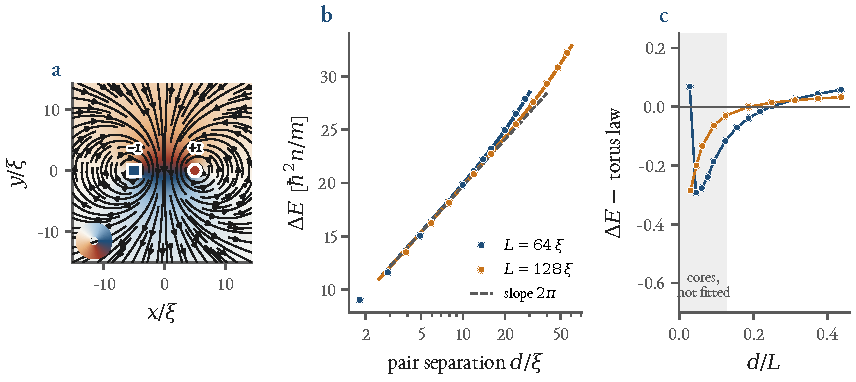
\includegraphics[width=\linewidth]{figures/ch06_coulomb.pdf}
\caption[The logarithmic interaction of vortices in the solver]{The logarithmic interaction of vortices in the solver. \textbf{a}~A vortex--antivortex pair (red disc: $+1$, blue square: $-1$), separation $d=10\,\xi$, imprinted into a
uniform condensate by \texttt{qf-pgpe} ($L=64\,\xi$); colour: phase of the field (the wheel at lower left), lines: streamlines of the superfluid velocity. \textbf{b}~Excess energy of
the imprinted pair against the separation, for $L=64\,\xi$ (blue) and $L=128\,\xi$ (orange); solid lines: the torus point-vortex law~\eqref{ch06:eq-torus} with one fitted
constant per box; dashed: the plane law with slope $2\pi$. \textbf{c}~Residual of the torus law; the shaded band is the core region $d<8\,\xi$ that was not fitted.
Source: \texttt{figures/ch06\_loglaw.py}, \texttt{ch06\_coulomb.py}.}\label{ch06:fig-coulomb}\end{figure}

For $d$ between $\cnDloSixtyfour$ and $\cnDhiSixtyfour$ $\xi$ ($\Delta E$ from $\cnElowSixtyfour$ to $\cnEhighSixtyfour$ in units $\hbar^2n/m$) in the box $L=64\,\xi$, and between
$\cnDloHundred$ and $\cnDhiHundred$ $\xi$ ($\Delta E$ from $\cnElowHundred$ to $\cnEhighHundred$) in $L=128\,\xi$, the engine follows~\eqref{ch06:eq-torus} with a single constant per
box to a root-mean-square deviation of $\cnRmsSixtyfour$ and $\cnRmsHundred$ (largest deviations $\cnMaxSixtyfour$ and $\cnMaxHundred$): about half a per cent of the
range of the energy in the root-mean-square, and less than one per cent at worst. The coefficient of the logarithm is tested more sharply by the constants: doubling the box changes $C_L$ by $2\pi\ln2=\cnTwoPiLnTwo$ if the coupling is
$2\pi\hbar^2n/m$, and the fitted constants differ by $\cnCdiff$ (the fit windows $d\ge4$, $6$, $8\,\xi$ give $\cnCdiffA$, $\cnCdiffB$, $\cnCdiff$). The naive slope of $\Delta E$ against $\ln d$ over the window $d=4$ to $8\,\xi$ is $\cnSlopeSixtyfour$ (box $64$) and
$\cnSlopeHundred$ (box $128$) times $2\pi$: the plane law is a good first guess, but the cores and the torus put a few per cent on it, and the comparison with the torus law is the
meaningful one. The Coulomb-gas coupling of the programme's projected field is therefore $2\pi\hbar^2n_s/m$ with $n_s=n$ at zero temperature, to within $0.3\%$ in the constants for every window tried, and
every instrument built on the point-vortex picture (the matching of \cref{ch06:field}, the pair statistics of \cref{ch07}) starts from a law that the engine itself obeys. The
imprint is not the relaxed vortex, so the constants themselves carry a core-mismatch energy; no claim is made about $E_c$.

\section{The flow, integrated by CVODE}\label{ch06:cvode}

\begin{rustbox}{CVODE on the Kosterlitz flow}
The flow~\eqref{ch06:eq-flow-u} is handed to CVODE through the Python module \texttt{rusty\_sundials}. Its \lstinline[style=py]{solve} returns only the end state, so a trajectory is
a chain of solves, each restarting the integrator from the previous end point (the drift reported below therefore includes the restarts). The excerpt is
verbatim from \texttt{figures/ch06\_flow\_compute.py} (\lstinline[style=py]{A_COEF} is $4\pi^3$; \lstinline[style=py]{H} is the invariant of \lean{KTFlow.kt\_invariant}; the last part is the body of the loop of the function
\lstinline[style=py]{chain}, one link of the chain per pass).
\begin{lstlisting}[style=py]
def f(u): return 2 * u - pi * math.log(u)
def H(u, y): return f(u) - 2 * pi ** 3 * y * y

def make_rhs(a=A_COEF):
    def rhs(l, s):
        u, y = s
        return [a * y * y, (2 - pi / u) * y]
    return rhs

def solver(method, rtol, atol=1e-13):
    return CvodeSolver(method=method, rtol=rtol, atol=atol, max_steps=500000)

    while l < lmax - 1e-12:
        step = dl
        if adaptive:
            step = min(dl, 0.05 / max(1.0, abs(rhs(l, s)[0])))
        l1 = min(l + step, lmax)
        try:
            _, s = sv.solve(rhs, l, s, l1)
        except RuntimeError:
            status = "solver_stop"; break
        l = l1
        L.append(l); U.append(s[0]); Y.append(s[1])
        if s[0] > ustop or abs(s[1]) > ystop:
            status = "left"; break
\end{lstlisting}
The module used for every number of this section is the build of rusty-SUNDIALS commit \cnCommitShort{} (\texttt{sha256} \cnShaShort{}\ldots, recorded in \texttt{figures/ch06\_numbers.json}). The script
refuses to run with any other: it first integrates $y'=-y$ on $[0,10]$ with Adams at $\mathrm{rtol}=10^{-8}$ and stops unless that needs fewer than $5000$ right-hand-side calls
($\cnPoneNew$ here). The printed record of the run (\texttt{figures/ch06\_flow\_compute.log}), last lines:
\begin{lstlisting}[style=plainmono]
adams_0.0001 2.2990858496996225e-05 0.020871856137751443 0.0
adams_1e-06 1.1391289778117653e-07 0.020866424221486657 0.1
adams_1e-08 2.703142154558691e-09 0.020866528666865003 0.3
adams_1e-10 1.9197976541818207e-11 0.02086653416968831 0.1
bdf_0.0001 6.019662951661786e-06 0.020866911425781565 0.2
bdf_1e-06 2.1762584490048198e-07 0.020866208945461207 0.8
bdf_1e-08 1.7298834809054142e-08 0.020866528311566324 1.0
bdf_1e-10 6.256666296167168e-10 0.020866533765439677 1.3
control [0.013523778528752306, 0.004224805752023997, 0.0009541671101744864, 0.011222398376601106, 0.2505532326600892, 0.01841533553023922]
\end{lstlisting}
(columns: method and \texttt{rtol}; the largest drift of $H$ over six trajectories to $l=40$; the smallest distance of those trajectories from $u=\pi/2$; the seconds of the run on the shared machine. Last
line: the drift of the same six trajectories of a flow whose coefficient $4\pi^3$ was changed by $5\%$ in $\dd u/\dd l$ only, the negative control.)
\end{rustbox}

\paragraph{A first-order integrator hiding in plain sight.} Our first attempt used the \texttt{rusty\_sundials} module that sits in the programme's virtual environment, and it was
slow in a way that smelled wrong: one link of $0.25$ units of $l$ cost $\cnPthreeOld$ evaluations of the right-hand side, and $20$ units cost $\cnPfourOld$. We counted. For a smooth,
slowly varying flow at $\mathrm{rtol}=10^{-9}$, a variable-order Adams method should need a few hundred. The module built from commit \cnCommitShort{} needs $\cnPthreeNew$ and
$\cnPfourNew$; on $y'=-y$ over $[0,10]$ at $\mathrm{rtol}=10^{-8}$ the old module needs $\cnPoneOld$ and the new one $\cnPoneNew$, and the old one's error is $\cnPoneOldErr$ against $\cnPoneNewErr$
(figures/ch06\_cvode\_probe.py, \texttt{ch06\_cvode\_probe\_venv.json} and \texttt{\_5db8041.json}). The old module had been built before a repair to the library: its
Adams method never left order one (it was implicit Euler with a Milne-style error estimate), and a first-order method under local error control has a global error that falls only like
the square root of the tolerance (\texttt{docs/CVODE\_ADAMS\_FIX.md} of rusty-SUNDIALS). Its answers are far less accurate than the tolerance that was asked for, and each costs a thousand times
more work; nothing in its output says so, and a user who does not count calls would not know. Our first full run with it had not finished the first of its six parts after ten minutes of
wall-clock time on the shared machine when we stopped it to count. The lesson is the programme's usual one: a solver result needs a cost figure next to it, and the script an environment check.

\paragraph{The portrait.} \Cref{ch06:fig-portrait}a shows $\cnNtraj$ trajectories integrated with Adams at $\mathrm{rtol}=10^{-9}$, drawn over the level sets of the exact invariant. Of
the $\cnNtraj$ starting points, $\cnNhyp$ satisfy the hypothesis of the trapping theorem ($u_0<\pi/2$, $H_0>f(\pi/2)$). All $\cnNhyp$ stay below $u=\pi/2$ for the whole run to $l=60$, $u$ is
monotone along each, and $y^2\le y_0^2$ throughout, as \Lthm{KTFlow}{kt_trapped}, \Lthm{KTFlow}{u_monotone} and \Lthm{KTFlow}{kt_fugacity_bounded} require; their end points lie on the line of fixed points at
the root $u_*$ of $f(u_*)=H_0$, as the invariant says they must: to $\cnUstarErrTypical$ or better for all but three of them, which start within $4\times10^{-3}$ of the separatrix in $H$ and have not
converged at $l=60$ (the worst differs from the root by $\cnMaxUstarErr$). The $\cnNbelow$ starting points on the superfluid side \emph{below} the separatrix all cross $u=\pi/2$ ($\cnNbelow$ of
$\cnNbelow$), as the new escape theorems require. And $\cnNbetween$ starting points lie between the exact separatrix and the textbook straight line $y=(\pi/2-u)/\pi^2$: the linearised
picture sends them to the disordered phase; the exact invariant, the theorem and CVODE all keep them on the superfluid side ($\cnNbetweenTrapped$ of $\cnNbetween$ trapped).

\begin{figure}[tbp]\centering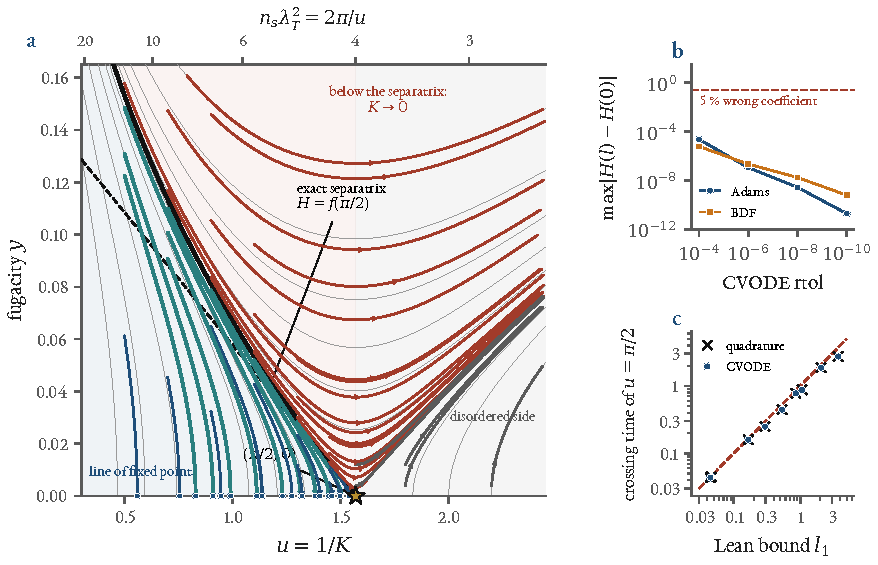
\includegraphics[width=\linewidth]{figures/ch06_portrait.pdf}
\caption[The Kosterlitz flow, integrated with CVODE]{The Kosterlitz flow, integrated with CVODE (rusty-SUNDIALS). \textbf{a}~Trajectories in the plane $(u=1/K,y)$ over the level sets of the exact invariant $H$ (thin grey lines;
by \Lthm{KTFlow}{kt_invariant} they are the flow lines). Blue: starting points that satisfy the hypothesis of \Lthm{KTFlow}{kt_trapped}; teal: those that lie between the exact separatrix
(black) and the textbook line (dashed); red: below the separatrix; grey: starting beyond $u=\pi/2$. Dots on the axis: the roots $u_*$ of $f(u_*)=H_0$. Star: the fixed point
$(\pi/2,0)$, $K=2/\pi$; the upper axis gives $n_s\lambda_T^2=2\pi/u$. \textbf{b}~Largest drift of $H$ over six trajectories ($l\le40$) against the CVODE tolerance for Adams and BDF, and for a flow with
a $5\%$ wrong coefficient (dashed red). \textbf{c}~Crossing time of $u=\pi/2$ below the separatrix, CVODE (dots) and the exact quadrature of the scalar equation (crosses), against the bound $l_1$
of \lean{kt\_escape\_time} (dashed: equality). Source: \texttt{figures/ch06\_flow\_compute.py}, \texttt{ch06\_portrait.py}.}\label{ch06:fig-portrait}\end{figure}

\paragraph{The invariant as a test of the integrator.} The theorem says $H$ is constant; the numerical $H$ is therefore a direct measurement of the global error of the integrator, with no
reference solution needed. \Cref{ch06:fig-portrait}b: with Adams the largest drift over six trajectories falls from $\cnDriftAdamsA$ at $\mathrm{rtol}=10^{-4}$ to $\cnDriftAdamsD$ at $10^{-10}$,
about as fast as the tolerance; with BDF from $\cnDriftBdfA$ to $\cnDriftBdfD$, slower at tight tolerance. The negative control shows the test has teeth: with the coefficient of $\dd u/\dd l$ wrong by $5\%$ the same
six trajectories drift by $\cnCtlLo$ to $\cnCtlHi$, that is, by $\cnCtlRatioLo$ to $\cnCtlRatioHi$ times the drift of the correct flow at the tightest tolerance. (The drift measured here includes the restart at every link; a
single call to a long interval does better, and we report the drift that a user of this interface gets.)

\paragraph{The escape bound.} For nine starting points below the separatrix (\cref{ch06:fig-portrait}c) we measure the first-passage time of $u$ through $\pi/2$ by root-finding on single CVODE solves,
and compare it with two things: the exact value of the quadrature $\int_{u_0}^{\pi/2}\dd u/(2(f(u)-H_0))$, which the scalar reduction \lean{kt\_scalar} makes available, and the Lean bound $l_1$.
CVODE and the quadrature agree to $\cnEscRelErr$ (relative), and the crossing time is below the bound in all $\cnEscN$ cases, at $\cnEscRatioLo$ to $\cnEscRatioHi$ of it. The bound uses the
smallest slope of $u$ on the way, $2(f(\pi/2)-H_0)$, which is attained only at $u=\pi/2$, so it is tight when the start is far below the separatrix and the slope is nearly the same all the way
(ratios near $1$ for the largest $f(\pi/2)-H_0$), and loose near the separatrix. This is one of the places where the proof assistant and the solver check each other: the theorem is quantitative,
and the solver tests the number.

\begin{figure}[tbp]\centering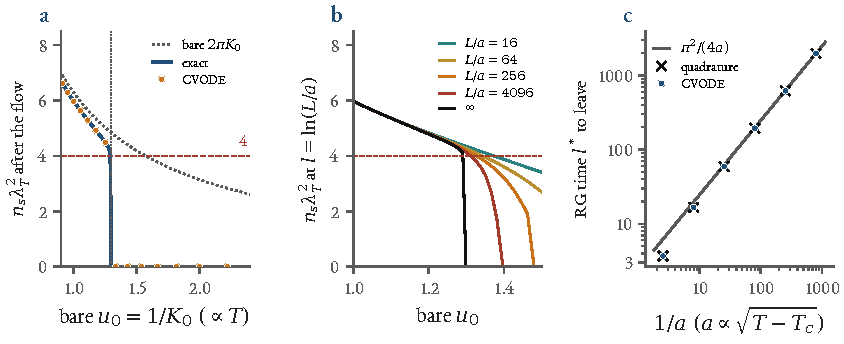
\includegraphics[width=\linewidth]{figures/ch06_jump.pdf}
\caption[The universal jump, the finite box and the essential singularity]{The universal jump, the finite box and the essential singularity in the flow (CVODE, Adams). \textbf{a}~Renormalised $n_s\lambda_T^2=2\pi K_R$ against the bare $u_0=1/K_0$ at fixed
$y_0=0.03$ (a toy: the bare fugacity is not tied to the temperature): the root of $f(u_*)=H_0$ (blue) and the end of a CVODE chain to $l=80$ (orange dots). The renormalised stiffness stays
above $4$ on the superfluid side and is $0$ beyond $u_{0c}$; the dotted curve is the bare $2\pi K_0$. \textbf{b}~The same flow stopped at $l=\ln(L/a)$, for four box sizes, and the limit $L\to\infty$:
the jump is rounded, and the crossing of the level $4$ moves to larger $u_0$ (higher temperature) in a smaller box. \textbf{c}~The scale $l^*$ at which a flow just above the separatrix leaves the critical
region, against $1/a$ with $a^2=(\pi/2)(f(\pi/2)-H_0)$, $a\propto\sqrt{T-T_c}$: CVODE (dots), quadrature (crosses), and the asymptote $\pi^2/(4a)$ (line): $\xi=e^{l^*}\sim e^{\pi^2/4a}$, the essential singularity. Source:
\texttt{figures/ch06\_flow\_compute.py}, \texttt{ch06\_jump.py}.}\label{ch06:fig-jump}\end{figure}

\paragraph{The jump.} \Cref{ch06:fig-jump}a puts the two halves of the theorem together for a one-parameter family of flows at fixed $y_0=0.03$ (a toy, the bare fugacity is not tied to the
bare stiffness here; the aim is the shape). On the superfluid side the end point of the flow is the root $u_*$ of $f(u_*)=H_0$ and the renormalised stiffness is above the universal value; the
end of a CVODE chain to $l=80$ agrees with the root (for $K_0=0.8$: $K_R=\cnKRcv$ from both). Past the critical bare stiffness, $K_{0c}=\cnKzeroC$ ($u_{0c}=\cnUzeroC$), $y$ grows and $K$ falls to zero.
Just above $K_{0c}$ the renormalised stiffness is $K_R=\cnKRgrid$ ($n_s\lambda_T^2=\cnNslGrid$) at the nearest grid point, and tends to the universal value $2/\pi$ with a square-root cusp:
$f(u)\simeq f(\pi/2)+(2/\pi)(u-\pi/2)^2$ gives $K_R-2/\pi\simeq(4/\pi^2)\sqrt{\pi\epsilon/2}$ for $H_0=f(\pi/2)+\epsilon$. This continuity is the third piece of the jump, the one that the theorems do not prove. The jump itself, from $4$ to $0$, is what Bishop and Reppy tested.

\paragraph{A finite box.} A film of size $L$ cannot flow further than $l=\ln(L/a)$. \Cref{ch06:fig-jump}b stops the flow there. The jump is rounded, and the apparent transition, the crossing of
$n_s\lambda_T^2=4$, moves to a larger bare $u_0$, that is, a higher temperature: by $\cnShiftA$, $\cnShiftB$, $\cnShiftC$ and $\cnShiftD$ of $u_{0c}$ for $L/a=16$, $64$, $256$ and $4096$. The reason
is the approach to the fixed point along the separatrix. With $x=u-\pi/2<0$ the scalar equation becomes $x'=(4/\pi)x^2(1+O(x))$, so $x\simeq-\pi/(4l)$ and
\begin{equation}
  n_s\lambda_T^2(l)=\frac{2\pi}{u}\simeq4+\frac{2}{l}\qquad\text{along the critical trajectory}
  \label{ch06:eq-critical}
\end{equation}
(Exercise~2): the critical film still looks stiffer than $4$ at any finite scale, and only logarithmically so. CVODE agrees: $l\,(n_s\lambda_T^2-4)$ along the separatrix is
$\cnCritA$ at $l=10$, $\cnCritB$ at $l=10^2$ and $\cnCritC$ at $l=10^4$, tending to $2$, with the invariant conserved to $\cnCritDrift$ over the whole run.

\paragraph{Above the transition.} For a flow that starts just below the separatrix, $H_0=f(\pi/2)-\epsilon$, the scalar equation near the fixed point is $x'=(4/\pi)(x^2+a^2)$ with
$a^2=(\pi/2)\epsilon$, and the time to cross from $-X$ to $X$ is $(\pi/4a)\,2\arctan(X/a)\to\pi^2/(4a)$: the flow lingers at the fixed point for a time that diverges as $1/\sqrt{\epsilon}$, and since
$\epsilon$ is linear in the distance from the critical temperature, the correlation length $\xi\sim e^{l^*}$ diverges as $\exp(b/\sqrt{T-T_c})$. \Cref{ch06:fig-jump}c: the time for the flow to
reach $u=2$ from $u_0=0.8$, by quadrature and by CVODE, divided by $\pi^2/(4a)$ is $\cnEssRatioA$, $\cnEssRatioB$ and $\cnEssRatioC$ for $\epsilon=10^{-1}$, $10^{-3}$ and $10^{-6}$; the difference
$l^*-\pi^2/(4a)$ settles at $-\cnEssOffset$, a constant that depends on where one chooses to stop. CVODE and the quadrature differ by $\cnEssRel$ (relative) at the smallest $\epsilon$.

The flow equations are a model; everything so far says that the model is internally consistent with the theorems and that CVODE integrates it correctly. Whether a fluid obeys it is another question,
and the next section asks it of the solver's own fluid.

\section{The simulated field near the transition}\label{ch06:field}

The engine of \cref{ch06:coulomb} is a classical field: the projected Gross--Pitaevskii equation, started from a random state of chosen total energy, thermalises, and its
temperature is \emph{measured} from the trajectory (equipartition of the modes near the cutoff), not imposed. It is a weakly interacting Bose gas with a cutoff, not helium; the
Kosterlitz--Thouless mechanism needs only a stiff phase and vortices, and the field has both (this is the property the analogy with the film depends on, in the sense of the
programme's rule LL-15), but a number measured here is a number of this model. The \emph{heating ladder} of the programme's second round starts from two equilibrated cold states (energy per particle $e=0.90$, evolved to $t=4000$, two seeds), adds random phonons
until the total energy reaches the target, and raises $e$ in nine steps, $e=1.00,1.05,\dots,1.40$, in a periodic box of side $L=64\,\xi$; each run has a transient of $500$ time units and is
averaged over $t=500$ to $1500$ (\texttt{data/generated/pgpe/r2/}, files \texttt{II\_*.json}). The steps above $e=1.20$ were added after the log of the first runs showed that the crossing
lay above the range that had been pre-registered (amendment R2-A4 of the programme, written before any verdict was computed). A smaller box, $L=32\,\xi$, with five energies and three
seeds, was run to see the size dependence; those runs start from random states and last $4000$ time units, with the last $1000$ sampled, so the comparison of the two boxes inherits
a difference of protocol. For each run we recompute from the saved per-run records (\texttt{figures/ch06\_pgpe\_data.py}, which agrees with the programme's own analysis to the last digit)
\begin{itemize}
\item $T$, from equipartition of the high-wavenumber modes, in units $\hbar^2/(m\xi^2)$ with $k_B=1$;
\item $n_s/n$, from the transverse and longitudinal current correlators at the smallest wavevectors, $n_s/n=1-\langle|J_T|^2\rangle/\langle|J_L|^2\rangle$, and from it
$n_s\lambda_T^2=(n_s/n)\,2\pi/T$ (for $n=1$, $\lambda_T^2=2\pi/T$);
\item $\eta$, from a fit of $g_1(r)\sim r^{-\eta}$ over a window that excludes the noise floor;
\item the vortices, by the winding rule of \lean{VortexWinding} (the sum of the principal-value phase differences around a plaquette is an exact multiple of $2\pi$).
\end{itemize}
Only runs that pass the programme's equilibrium admission test (the longitudinal and transverse current fluctuations must not exceed what an equilibrium state allows) enter; all 18
runs of the $L=64$ ladder and all 15 of the $L=32$ series pass. \Cref{ch06:tab-ladder} gives the seed means.

\begin{table}[t]\centering\small
\caption{The heating ladder, $L=64\,\xi$: seed means of $T$, superfluid fraction, $n_s\lambda_T^2$, the exponent $\eta$ of $g_1$, the product $\eta\,n_s\lambda_T^2$ (equal to $1$ for a
Gaussian phase field, \cref{ch06:eq-eta}), and the number of vortices (all runs, both signs). Source: \texttt{figures/ch06\_pgpe\_numbers.json}.}\label{ch06:tab-ladder}
\begin{tabular}{@{}rrrrrrr@{}}\toprule
$e$ & $T$ & $n_s/n$ & $n_s\lambda_T^2$ & $\eta$ & $\eta\,n_s\lambda_T^2$ & $N_v$\\\midrule
% BEGIN ch06 table
1.00 & 0.571 & 0.809 & 8.90 & 0.126 & 1.12 & 19\\
1.05 & 0.622 & 0.767 & 7.75 & 0.145 & 1.12 & 32\\
1.10 & 0.668 & 0.725 & 6.82 & 0.164 & 1.12 & 47\\
1.15 & 0.722 & 0.703 & 6.11 & 0.192 & 1.18 & 66\\
1.20 & 0.775 & 0.647 & 5.24 & 0.230 & 1.20 & 90\\
1.25 & 0.818 & 0.533 & 4.09 & 0.297 & 1.22 & 117\\
1.30 & 0.862 & 0.370 & 2.70 & 0.447 & 1.21 & 147\\
1.35 & 0.906 & 0.357 & 2.48 & 0.540 & 1.34 & 179\\
1.40 & 0.966 & 0.255 & 1.66 & 0.660 & 1.09 & 212\\
% END ch06 table
\bottomrule\end{tabular}\end{table}

\Cref{ch06:fig-field}d shows the stiffness. It falls through the Nelson--Kosterlitz level $n_s\lambda_T^2=4$ between $e=1.25$ and $e=1.30$; interpolating the seed means, the crossing
is at $T_{\rm BKT}(L{=}64)=\cnTbktSixtyfour$, where $\eta=\cnEtaCrossSixtyfour$ (the infinite-size value is $1/4$) and $n_s/n=\cnNsOverNCross$. The two seeds do not agree on where the
crossing is: taken separately they give $\cnTbktSeedLo$ and $\cnTbktSeedHi$; this is the honest error bar of the number. At $e=1.25$ the two seeds read $n_s\lambda_T^2=\cnKseedA$ and
$\cnKseedB$, on either side of $4$. In the smaller box the crossing is at $T_{\rm BKT}(L{=}32)=\cnTbktThirtytwo$ (seeds: $\cnTbktSeedLoThirtytwo$ to $\cnTbktSeedHiThirtytwo$, which does not overlap the
range of the larger box), and the fall of the stiffness is gentler: the slope $|\dd(n_s\lambda_T^2)/\dd T|$ at the crossing is $\cnSlopeCrossSixtyfour$ for $L=64$ and $\cnSlopeCrossThirtytwo$ for
$L=32$. Both signs, a crossing at a higher temperature and a softer fall in the smaller box, are what the flow predicts when it is stopped at the scale of the box: a film of size
$L$ sees the stiffness $K(l)$ at $l=\ln(L/a)$, and along the critical trajectory this exceeds $2/\pi$ by an amount that shrinks only as $1/l$ (\cref{ch06:fig-jump}b and
Exercise~2). The toy flow of that figure has two parameters that we did not fit to the field, and the agreement is one of sign and not of number: between $L/a=32$ and $64$ the toy moves the crossing, in temperature, by $\cnShiftToy\%$, and the field
between $L=32\,\xi$ and $64\,\xi$ by $\cnShiftField\%$.

\begin{figure}[t]\centering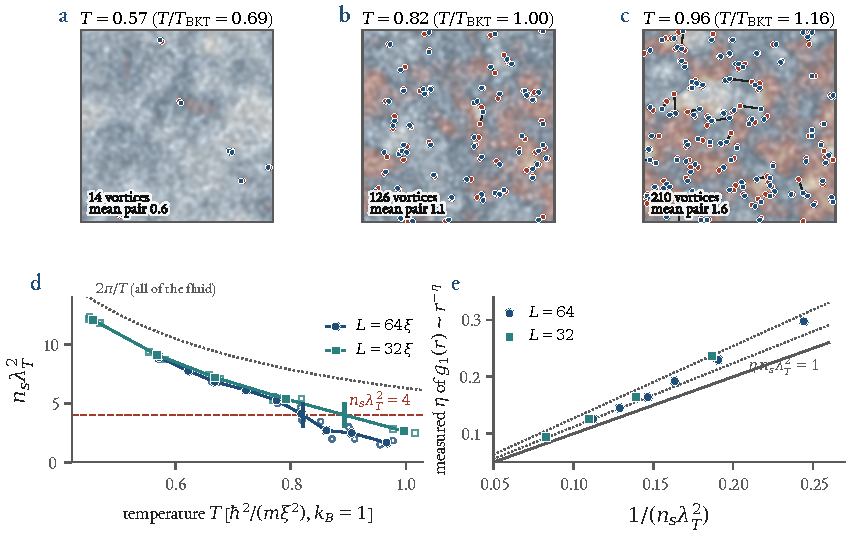
\includegraphics[width=\linewidth]{figures/ch06_field.pdf}
\caption[The simulated Bose field near the transition]{The simulated Bose field near the transition. \textbf{a--c}~Final states of the $L=64\,\xi$ heating ladder at $T=0.57$, $0.82$ and $0.96$ (in units of
$T_{\rm BKT}(64)=0.82$: $0.69$, $1.00$, $1.16$): vortices ($+1$ red, $-1$ blue) found by the winding rule, the optimal pairing of positive to negative vortices as black bonds, and
the coarse-grained phase as background hue; positions are on the grid, so separations below $0.5\,\xi$ are not resolved. \textbf{d}~$n_s\lambda_T^2$ against $T$: single runs (open
symbols) and seed means (filled) for $L=64$ (blue) and $L=32$ (teal); the red dashed line is the universal level $4$, the ticks mark the interpolated crossings, the dotted line is
$2\pi/T$, the value if the whole fluid were superfluid. \textbf{e}~Measured $\eta$ against $1/(n_s\lambda_T^2)$ for the energies with $n_s\lambda_T^2>4$; the grey line is the
spin-wave relation $\eta\,n_s\lambda_T^2=1$, the dotted lines are $12$ and $27\%$ above it. Source: \texttt{figures/ch06\_field.py}.}\label{ch06:fig-field}\end{figure}

\paragraph{What does not come out as the theory says.} Three things. First, the classical field at the crossing has $n\lambda_T^2=2\pi/T_{\rm BKT}=\cnNlambda$, against
$\ln(380/\tilde g)=\cnLnThreeEighty$ for the weakly interacting gas without a cutoff (Prokof'ev, Ruebenacker and Svistunov~\cite{Prokofev2001}; $\tilde g=1$ here, which is not small):
$\cnNlambdaExcess\,\%$ more. The programme's literature review suggested that this is the ultraviolet logarithm of a classical field with a sharp cutoff; the estimate it gives for our cutoff,
$T_{\rm BKT}=0.811$ and $n\lambda_T^2=7.75$, is close to the measured values, but that was a hypothesis when this chapter was written, not a test, and we do not use it. Second, the
spin-wave relation. For the six energies with $n_s\lambda_T^2>4$ the product $\eta\,n_s\lambda_T^2$ is $\cnEtaKlo$ to $\cnEtaKhi$ (\cref{ch06:fig-field}e), and for $L=32$ it is
$\cnEtaKloThirtytwo$ to $\cnEtaKhiThirtytwo$: a systematic excess of $12$ to $27\%$ over $1$, which is outside the scatter of the seeds. The programme's larger boxes ($L=128$ and $192$) show an
excess that is also positive at every size and not monotone in $L$; its origin is unknown to us, and \cref{ch10} lists it among the open items. Third, the round-1 value
$T_{\rm BKT}\approx0.72$, interpolated between states that were started by a quench, is withdrawn: those states were not equilibrated (at the same vortex count they had half the
stiffness of the heated ones), and $0.821$ replaces it.

\paragraph{Vortex positions against the two Lean statements.} \Cref{ch06:fig-field}a--c show what the optimal pairing looks like. At the lowest temperature almost all vortices are
in tight pairs (the mean matched separation is $\cnPairLo\,\xi$, at the resolution of the grid); at $T_{\rm BKT}$ there are $\cnNvMid$ vortices in the box with a mean matched
separation of $\cnPairMid\,\xi$; at $T=0.96$ the pairs are $\cnPairHi\,\xi$ long and the bonds begin to reach across the box. We now apply the two statements of \cref{ch06:lean} to
every configuration at hand: the final fields of the two series ($33$ configurations) and the saved positions of six $L=192$ runs ($100$ snapshots each, $t=13\,510$ to $14\,500$, the last window of the programme's longest runs; five of the six are equilibrated, the sixth, $e=1.10$ seed $11$, still carries one pair
of the size of the box). For each configuration we find the optimal matching $W$ with minimum-image distances, and evaluate $|\rho(k)|/|k|$ on the
reciprocal lattice (all $|n_x|,|n_y|\le6$).

\begin{figure}[t]\centering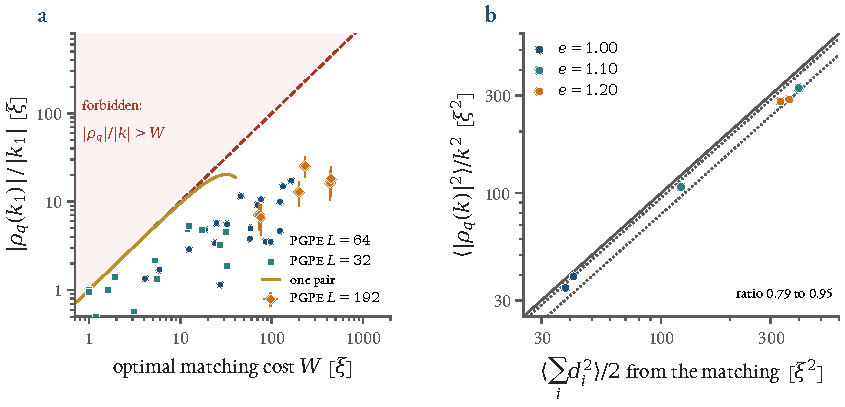
\includegraphics[width=\linewidth]{figures/ch06_screening.pdf}
\caption[The two Lean statements about vortex positions, tested on the solver's configurations]{The two Lean statements about vortex positions, tested on the solver's configurations. \textbf{a}~$|\rho_q(k_1)|/|k_1|$ at the smallest wavevector against the optimal
matching cost $W$: $33$ final fields of the $L=64$ and $L=32$ series (symbols), the six $L=192$ runs (mean and standard deviation over $100$ snapshots), and one isolated pair of
separation $d$ in a box of $64\,\xi$ (gold curve). The red dashed line is the bound of \Lthm{MatchingScreening}{norm_rho_le_matching_torus}: no point may lie above it, and none does. \textbf{b}~The polarisability
plateau $\langle|\rho_q(k)|^2\rangle/k^2$ (mean over the shells $m^2=4,\dots,16$) against $\langle\sum_id_i^2\rangle/2$ from the optimal matching, for the six $L=192$ runs; the dotted
lines are $0.79$ and $0.95$ times the diagonal. Source: \texttt{figures/ch06\_certificates.py}, \texttt{ch06\_screening.py}.}\label{ch06:fig-screening}\end{figure}

\emph{The matching bound.} There is no violation in any of the $\cnNconfigs$ configurations, nor in any of the $600$ snapshots of the $L=192$ runs, on any of the wavevectors tried.
That the inequality holds is no surprise, since it is a theorem; what the data show is how much room it leaves. For a thermal gas of tight pairs the bound is loose: the ratio
$\tau=|\rho(k_1)|/(|k_1|W)$ is $\cnTauLoFields$ to $\cnTauHiFields$ for the fields (the large values are the configurations with one or two pairs) and $\cnTauLoRuns$ to $\cnTauHiRuns$ for the
$L=192$ runs, because the pairs cancel each other's charge at a long wavelength while the matching cost counts every one of them. The bound is saturated only by an isolated pair
whose separation is small against the wavelength, $\tau=\sin(k_1d/2)/(k_1d/2)\to1$ (Exercise~3). It is a certificate, not a detector: it bounds the total pairing length from below
whatever the configuration (a charge density of order one at the smallest wavevector requires the vortices of opposite sign to be, in total, at least $L/2\pi$ apart), and a small value
certifies nothing.

\emph{The polarisation form.} At the four shortest wavevectors the premise $|k\cdot d_i|\le1$ of \Lthm{PairPolarisation}{rho_polarisation} holds for every pair in $\cnPremiseOk$ of the $\cnNconfigs$ field
configurations, and in all of them the inequality $|\rho-i\sum_i(k\cdot d_i)e^{ik\cdot m_i}|\le\sum_i(k\cdot d_i)^2$ holds, with the pairs taken from the optimal matching. The typical size of the remainder
is $\cnRemMed$ of $|\rho|$ (median), and the bound on it is $\cnBoundMed$ of $|\rho|$: in a thermal gas of pairs the long-wavelength vortex charge density is, to about
$\cnRemMedPct\,\%$ (median over the configurations), the divergence of a polarisation density. That is the dielectric picture in numbers. Its consequence for the stiffness is Kosterlitz and Thouless's $\varepsilon-1\propto\sum d^2$,
and \cref{ch06:fig-screening}b checks it on the six $L=192$ runs: the long-wavelength charge fluctuations per $k^2$ are $\cnDfourLo$ to
$\cnDfourHi$ of the sum of $d_i^2/2$ over the matched pairs, always below it; the programme reads the deficit as the screening of dipoles by dipoles, which we did not test separately. We re-derived these numbers with independent code, because the file stored in the repository
for them (\texttt{data/generated/pgpe/dielectric/primary\_C4.json}) still holds the values from before a correction, about $0.009$ (a factor $k^2$ applied by mistake, as
\texttt{PGPE\_DIELECTRIC\_RESULTS.md} records); our values match the corrected table of that document. What the dielectric analysis does \emph{not} give is a mode-by-mode relation between the
transverse current and the detected charges: the pre-registered test of that failed in five of six runs, the coherence being $0.06$ to $0.28$.

\section{What this chapter establishes, and what it does not}\label{ch06:honest}

\begin{honestbox}
\textbf{Proved in Lean} (kernel-checked; every declaration depends only on \texttt{propext}, \texttt{Classical.choice}, \texttt{Quot.sound}). In the library: the exact invariant and the trapping
of the Kosterlitz flow, the monotonicity of $u$, the bound on the fugacity and the unit conversion ($K>2/\pi\iff n_s\lambda_T^2>4$) \emph{for solutions defined for every real $l$}; the bound of
the vortex charge density by every pairing of the vortices (plane and torus); the polarisation form of the charge density of pairs. In the new module of this book
(\texttt{book/lean/Ch06\_KTForward.lean}, $18$ declarations audited, no \lstinline[style=lean]{sorry}): the same statements for solutions on $l\ge0$ only, the escape bound and escape time below the separatrix,
the vanishing of $K$ there, the dichotomy at the separatrix, and the theorem that the library's hypotheses leave only fixed points on the superfluid side. \emph{Not} formalised: that non-trivial
solutions on $[0,\infty)$ exist; that $K_R\to2/\pi$ as the invariant tends to $f(\pi/2)$ from above; the flow equations themselves, which are Kosterlitz's leading-order equations, taken as given.

\textbf{Computed} (CVODE from rusty-SUNDIALS commit \cnCommitShort{}; \texttt{qf-pgpe} as installed on the machine, its build commit not recorded; one shared, loaded machine). CVODE integrates the flow with the invariant conserved to $\cnDriftAdamsD$ (Adams, $\mathrm{rtol}=10^{-10}$, chain of
solves), reproduces the exact first-passage times to $\cnEscRelErr$ and keeps all $\cnNhyp$ trapped starting points trapped; the engine \texttt{qf-pgpe} follows the torus point-vortex law for the energy of an imprinted
pair to a root-mean-square deviation of $\cnRmsSixtyfour$ ($L=64$) and $\cnRmsHundred$ ($L=128$) in units of $\hbar^2n/m$, and the coefficient $2\pi\hbar^2n/m$ of the logarithm to $0.3\%$. The classical field has an
$n_s\lambda_T^2$ that crosses $4$ at $T_{\rm BKT}(64)=\cnTbktSixtyfour$ (seeds $\cnTbktSeedLo$ to $\cnTbktSeedHi$) and $T_{\rm BKT}(32)=\cnTbktThirtytwo$; these come from runs of the programme's numpy engine
(two seeds for $L=64$, three for $L=32$), recomputed here from the raw records, not re-run. The two Lean statements about vortex positions were tested on $\cnNconfigs$ configurations and $600$ snapshots and are
never violated.

\textbf{Measured.} The only experiment of this chapter is Bishop and Reppy's, as its abstract reports it: no film data were analysed, and nothing here is a statement about helium except that jump formula and the
number $\cnJump\times10^{-9}\ \mathrm{g\,cm^{-2}\,K^{-1}}$ computed from it. The simulated field is a classical Bose gas with a cutoff, in units where $\tilde g=1$ is not small; the match with a film is the
shared mechanism (a stiff phase with vortices), not a quantitative identity. The Godfrin measurements are of a different system (a Fermi liquid) and enter only through the dimension.

\textbf{Analogy, not result.} The toy flow of \cref{ch06:fig-jump} gives the sign of the finite-size shift of the transition but about one per cent where the field shows nine; its bare parameters were not fitted.

\textbf{Failed, withdrawn or open.} (i)~The round-1 transition temperature $T_{\rm BKT}\approx0.72$ of the programme, from quench-started states, is withdrawn in favour of $0.821$ (the quench states were not equilibrated).
(ii)~The spin-wave relation $\eta\,n_s\lambda_T^2=1$ is violated by a systematic $12$--$27\%$ at $L=32$ and $64$, and by a positive and non-monotone amount at larger sizes; unexplained. (iii)~The programme's
pre-registered mode-by-mode relation between the transverse current and the detected vortex charges failed (five of six runs); only the polarisability plateau holds (ratios $\cnDfourLo$ to $\cnDfourHi$).
(iv)~$n\lambda_T^2$ at the crossing is $\cnNlambdaExcess\%$ above the weak-coupling value $\ln380$; the cutoff explanation was not tested. (v)~Seeds: two (or three) per point; the transition temperature is known to $\pm0.014$ ($L=64$)
at best. (vi)~\emph{Found while writing this chapter}: the hypotheses of the library theorems \lean{KTFlow} cover only fixed points on the superfluid side (the library file is unchanged; the repaired statements
live in the book's module); the Python CVODE module of the project's environment predates the Adams repair and costs a thousand times more per result, and the current build's \lstinline[style=py]{solve} does not handle an output
time before the initial time; and the file \texttt{primary\_C4.json} stores pre-correction values of the polarisability ratio.
\end{honestbox}

\section*{Exercises}

\paragraph{Exercise 1.} Show that for $\dd u/\dd l=c\,y^2$ and $\dd y/\dd l=(2-\pi/u)\,y$, with any constant $c>0$, the function $2u-\pi\ln u-\tfrac c2\,y^2$ is conserved. Expand it
near $(\pi/2,0)$ and show that the level sets are the hyperbolas $x^2-(\pi c/4)\,y^2=\mathrm{const}$, $x=u-\pi/2$, with straight separatrices $y=\pm x/\pi^2$ for $c=4\pi^3$. What changes in the
statement of the trapping theorem if $c$ is replaced by another constant? \emph{Hint:} differentiate; $f''(\pi/2)=4/\pi$, so $f(u)\simeq f(\pi/2)+(2/\pi)x^2$.

\paragraph{Exercise 2.} Prove~\eqref{ch06:eq-critical}: along the separatrix $n_s\lambda_T^2(l)=4+2/l+o(1/l)$, and more precisely $l\,(n_s\lambda_T^2-4)=2-\tfrac23\,(\ln l)/l+O(1/l)$. \emph{Hint:} on the separatrix
$H=f(\pi/2)$ and the scalar equation gives $x'=2\big(f(\pi/2+x)-f(\pi/2)\big)=(4/\pi)x^2-(16/3\pi^2)x^3+\dots$; integrate $\dd(1/x)/\dd l=-x'/x^2$, first with the leading term
($1/x\simeq-4l/\pi$), then once more to get the logarithm; then $2\pi/u=4/(1+2x/\pi)$. Compare with the values of $l\,(n_s\lambda_T^2-4)$ quoted in \cref{ch06:cvode}: the expression
$2-\tfrac23(\ln l)/l$ differs from them by $\cnCritDevB$ at $l=100$ and by $\cnCritDevC$ at $l=10^4$.

\paragraph{Exercise 3.} For one vortex--antivortex pair of separation $d$, show that $|\rho(k)|/|k|=2\sin(kd/2)/k$ when $k\parallel d$, hence that the ratio $\tau=|\rho(k)|/(|k|\,W)$ of
\Lthm{MatchingScreening}{norm_rho_le_matching} equals $\sin(kd/2)/(kd/2)$. Evaluate it for the smallest wavevector $k_1=2\pi/L$ of a box of side $L$ and a pair of size $d=L/2$, and compare with the gold
curve of \cref{ch06:fig-screening}a. Why can $\tau$ be close to $1$ only when $kd\ll1$, and what does that say about reading a small charge structure factor as evidence for short pairs?
\emph{Hint:} $|e^{i\varphi}-1|=2|\sin(\varphi/2)|$.

\section*{Notes and further reading}

The unbinding of vortex pairs as the mechanism of the two-dimensional transition is due to Kosterlitz and Thouless~\cite{KosterlitzThouless1973}; Berezinskii analysed the low-temperature state of
two-dimensional systems with a continuous symmetry independently~\cite{Berezinskii1971}, and the absence of long-range order they build on is the theorem of Mermin and
Wagner~\cite{MerminWagner1966} and of Hohenberg~\cite{Hohenberg1967}. The flow equations are Kosterlitz's~\cite{Kosterlitz1974}, the universal jump is Nelson and Kosterlitz's~\cite{NelsonKosterlitz1977},
and the experiment on helium films is Bishop and Reppy's~\cite{BishopReppy1978}, analysed with the dynamic theory of Ambegaokar, Halperin, Nelson and Siggia~\cite{AHNS1978,AHNS1980}. Minnhagen's
review~\cite{Minnhagen1987} covers the Coulomb gas, Kosterlitz's equations and the experiments on helium films, in the language used here. The same crossover was later studied in a trapped atomic gas~\cite{Hadzibabic2006};
the critical phase-space density of the weakly interacting gas is the subject of~\cite{Prokofev2001,ProkofevSvistunov2002}; classical-field simulations of the pairing and unbinding of vortices
are those of Simula and Blakie~\cite{SimulaBlakie2006} and of Foster, Blakie and Davis~\cite{FosterBlakieDavis2010}; Hasenbusch's Monte Carlo study of the XY model at the transition~\cite{Hasenbusch2005}
derives and tests the finite-size behaviour of the helicity modulus there. For point vortices on a torus see Weiss and McWilliams~\cite{WeissMcWilliams1991}. The records of the programme behind this chapter are, in the
repository, \texttt{LEDGER.md} (CLAIM-072 for \lean{KTFlow}, CLAIM-070 and CLAIM-085 for the vortex-position statements and the dielectric analysis), \texttt{docs/designs/PGPE\_R2\_RESULTS.md} (the ladder),
\texttt{PGPE\_DIELECTRIC\_RESULTS.md} and \texttt{PGPE\_ONSAGER\_RESULTS.md}. The friction and diffusion of a single vortex in the same field are the subject of \cref{ch07}.
}
\IfCh{ch07}{\chapter{Friction, Diffusion and the Dissipative Vortex}\label{ch07}
\raggedbottom% this chapter has long unbreakable code boxes and floats: let a page end short rather than stretch the glue; restored at the end of the chapter
\edef\chsevenwp{\the\widowpenalty}\edef\chsevencp{\the\clubpenalty}\widowpenalty=10000 \clubpenalty=10000 % no widows or orphans in this chapter; restored at its end

\section{A pair that opens, a pair that closes}\label{ch07:intro}

In an oblate sodium condensate two vortices of the same sign circle each other, and the pair is seen to open up: its separation grows with time, and grows faster in a warmer
cloud~\cite{Moon2015}. Read through a dissipative point-vortex model, the opening rate is a friction coefficient $\alpha$ between $0.01$ and $0.03$ over the
$200$--$450$~nK explored. In a rubidium condensate in a hard-walled optical trap, a crystal of vortices placed by optical tweezers and then released expands for the same reason;
fitting the expansion to a scaling law gives $\alpha=3.3(1)\times10^{-3}$, while the random wandering of the same vortices is about a hundred times larger than the theory that ties
it to the friction predicts, a surplus that the authors consider most likely due to vibrations of the trap walls~\cite{Neely2024}. Two things are read from the motion of a vortex: how
hard it is dragged, and how hard it is kicked.

Both come from one fact: a vortex in a warm superfluid is not alone. Around it is a gas of thermal excitations, the normal component of Landau's two-fluid
description~\cite{Landau1941}, and the vortex and the gas exchange momentum, which is called \emph{mutual friction}~\cite{Donnelly1991,Sergeev2023}. The gas acts on the vortex with a force along
its velocity relative to the gas and a force across it, and, when the gas is also the heat bath of the vortex, a third effect, random kicks, has to be added: three numbers, $\alpha$, $\alpha'$ and
$\eta$ (\cref{ch07:model}). This chapter follows the model through the three instruments of the book, in a classical field that has no walls, no reservoir and no noise put in by hand, so that the bath
of a vortex is the field's own thermal phonons.

The programme's record on these questions is mixed, and it is told as it stands in the ledger. What survives: the friction of a vortex pair in the field, $\alpha=0.0062(4)$ at
$T/T_{\rm BKT}=0.14$, read by two independent estimators, and a transverse coefficient that is zero to about one per cent. What the programme's own pre-registered tests refuted: the reading of
the friction as proportional to the normal density with a coefficient that belongs to the vortex; the explanation of a stalled single pair by the phonon wind of a closed box; and, earlier, a
known-answer gate that had seemed to pass on a defective instrument. What the decision rule written before the data leaves undecided: the Einstein relation between diffusion and friction.
And one finding is a bias in the very estimator that Lean proves exact in the model: a lesson about hypotheses, not about Lean.

\section{The dissipative point vortex}\label{ch07:model}

Work in units $\hbar=m=1$, so that the circulation quantum is $\kappa=2\pi$, in the frame where the normal component is at rest. A vortex of charge $q=\pm1$ is carried by the superfluid
velocity $\mathbf v_s$ that the other vortices induce at its position; the gas adds a drag along the velocity of the vortex relative to the gas and a force across it. In the two-fluid
equations of Hall, Vinen, Bekharevich and Khalatnikov these are the coefficients $\alpha$ and $\alpha'$~\cite{Shukla2014}, and for a weakly damped vortex they give
\begin{equation}
  \dot{\mathbf r}_i=(1-\alpha')\,\mathbf v_{s,i}-\alpha\,q_i\,\hat{\mathbf z}\times\mathbf v_{s,i}.
  \label{ch07:eq-motion}
\end{equation}
The second term is perpendicular to $\mathbf v_s$ and \emph{dissipative}: it carries energy from the vortices to the gas, and $\alpha$ is the friction. The factor $1-\alpha'$ only rescales the speed with which the
vortex follows the superfluid and dissipates nothing.

The structure of~\eqref{ch07:eq-motion} is clearest in terms of an energy. For point vortices on the plane $H=-\sum_{i<j}q_iq_j\ln r_{ij}^2$ (on the periodic box of the simulations, $\ln r^2$ is
replaced by the Weiss--McWilliams periodic Green function~\cite{WeissMcWilliams1991}; nothing below depends on it), and $\mathbf v_{s,i}=-\tfrac12 q_i\,\hat{\mathbf z}\times\nabla_iH$. Since $q_i^2=1$,
the friction term is $-\tfrac{\alpha}{2}\nabla_iH$, and the whole configuration obeys
\begin{equation}
  \dot{\mathbf r}\;=\;A(\nabla H)\;-\;\tfrac{\alpha}{2}\,\nabla H,
  \qquad \langle \mathbf v,A\mathbf v\rangle=0\ \text{ for every }\mathbf v,
  \label{ch07:eq-flow}
\end{equation}
a skew part $A$, which contains $\alpha'$ and moves the vortices along level sets of $H$, plus a gradient flow that moves them down $H$. Friction therefore pushes the members of an
opposite-sign pair together, because their energy $\ln d^2$ grows with the separation $d$, and pushes the members of a same-sign pair apart, because their energy $-\ln d^2$ falls as $d$ grows: the
first is the dipole that shrinks in the computer, the second the pair that opens in the sodium cloud.

\begin{keybox}[Three numbers describe a vortex in a warm fluid]
\textbf{$\alpha$} (friction): the vortex is dragged and energy flows from the vortices to the gas. \textbf{$\alpha'$} (transverse coefficient): the gas pushes the vortex sideways, without dissipation.
\textbf{$\eta$} (diffusion): the vortex is also kicked at random, $\langle|\Delta\mathbf r|^2\rangle=4\eta t$. If the gas is the heat bath of the vortex, an Einstein relation
$\eta=\alpha T/(2\pi\rho)$ ($k_B=1$) ties the last to the first.
\end{keybox}

\paragraph{The sideways force.} Thouless, Ao and Niu derived the total non-dissipative transverse force on a vortex as the Magnus force proportional to the superfluid density, the core states not changing
it~\cite{ThoulessAoNiu1996}: the normal fluid exerts no extra sideways force and $\alpha'=0$. Iordanskii~\cite{Iordanskii1964} and later Sonin~\cite{Sonin1997} find a transverse force from
the scattering of thermal excitations, which the programme registered as $\alpha'=\rho_n/\rho$.

\paragraph{The random kicks.} Add independent white noise of diffusion constant $\eta$ to~\eqref{ch07:eq-motion}. Mehdi, Hope, Szigeti and Bradley derive $\eta=\alpha k_BT/(2\pi\hbar\rho_0)$
($\rho_0$ the two-dimensional number density) from a stochastic projected Gross--Pitaevskii theory and single out its measurement as an important test of stochastic point-vortex theory~\cite{Mehdi2023}.
A model of this form had been used for helium films by Ambegaokar, Halperin, Nelson and Siggia, with the noise motivated by fluctuation--dissipation arguments and not derived~\cite{AHNS1980}.

\begin{godfrinbox}{the excitations are the bath}
Phys.\ Rev.\ B \textbf{103}, 104516 (2021) reports inelastic neutron scattering on superfluid $^4$He at the ILL spectrometer IN5: the dispersion relation of the Landau elementary excitations, phonon, maxon and roton, and the thermodynamic
consequences~\cite{Godfrin2021}. Those excitations are the normal component of Landau's picture~\cite{Landau1941}, and in the kinetic theory of mutual friction the friction on a vortex is their scattering by the vortex~\cite{Sergeev2023}. What such a measurement fixes, for helium, is
what sets the scale of every number below: the energy $\varepsilon(k)$ of a thermal excitation, hence the population of the bath. In our classical field the model must supply the bath itself, and \cref{ch07:law} shows how little it resembles a quantum gas. The statements of his papers that the library formalises are in \cref{ch04,ch05}, not here.
\end{godfrinbox}

\section{What Lean proves about the model}\label{ch07:lean}

Three modules of the library concern this chapter, \lean{Dissipative\-Vortex\-Dynamics}, \lean{Einstein\-Relation} and \lean{Friction\-Kinetic} (a fourth, \lean{QuasiPeriodic\-Bound}, appears once); a small new module written for the book adds statements to the first. The
mathematics is elementary calculus, and the modules say so. The point is that the estimators used on the data are \emph{identities of the model}, with the hypotheses under which they
hold written where a machine can read them. Every theorem quoted here depends only on the three standard axioms \texttt{propext}, \texttt{Classical.choice} and \texttt{Quot.sound}: the library modules carry no
\texttt{\#print axioms} lines, so this was checked on 2026-10-09 by compiling scratch copies with one such line per theorem (Lean~4.34.0-rc2, the pinned Mathlib; no errors, no \texttt{sorry}).

The first theorem is general: any dynamics of the form~\eqref{ch07:eq-flow}, on any real inner-product space (any number of vortices, plane or torus), with $A$ pointwise skew.

\begin{leanbox}[unbreakable]{DissipativeVortexDynamics}
\begin{lstlisting}[style=lean,basicstyle=\ttfamily\footnotesize]
variable {X : Type*} [NormedAddCommGroup X] [InnerProductSpace ℝ X] [CompleteSpace X]
theorem energy_dissipation (H : X → ℝ) (gradH : X → X) (hH : ∀ x, HasGradientAt H (gradH x) x)
    (A : X → X) (hA : ∀ v, inner ℝ v (A v) = 0) (γ : ℝ) (r : ℝ → X)
    (hr : ∀ t, HasDerivAt r (A (gradH (r t)) - γ • gradH (r t)) t) (t : ℝ) :
    HasDerivAt (fun t => H (r t)) (-γ * ‖gradH (r t)‖ ^ 2) t := by
\end{lstlisting}
\nopagebreak[4]\smallskip\noindent\textit{(Proof abridged: eleven lines in the module, the chain rule and then \texttt{hA}.)}
\end{leanbox}

In words: along any solution, $\frac{d}{dt}H=-\gamma\|\nabla H\|^2$, \emph{whatever the skew part}. For~\eqref{ch07:eq-motion}, $\gamma=\alpha/2$ and $\|\nabla H\|^2=4\sum_i|\mathbf v_{s,i}|^2$, hence
\begin{equation}
  \frac{dH}{dt}=-2\alpha\sum_i|\mathbf v_{s,i}|^2,\qquad
  \alpha_{\rm energy}=-\frac{\Delta H}{2\int\sum_i|\mathbf v_{s,i}|^2\,dt}.
  \label{ch07:eq-energy}
\end{equation}
The right-hand side estimates $\alpha$ from the positions of the tracked vortices alone, needs no pairing of them, and is blind to $\alpha'$ (\Lthm{DissipativeVortexDynamics}{dissipation_indep_of_skew}). This is the programme's
\emph{energy estimator}. Its hypothesis, written in the statement, is \texttt{hr}: the path has a derivative at every time. We shall come back to it.

For the plane dipole the model can be written in coordinates. Let $\mathbf p$ be the $+$ vortex, $\mathbf m$ the $-$ vortex, $\mathbf d=\mathbf p-\mathbf m$ and $\texttt{r2}=|\mathbf d|^2$; the superfluid velocity at either vortex is $(d_y,-d_x)/\texttt{r2}$.
The hypotheses \texttt{hpx}, \texttt{hpy}, \texttt{hmx}, \texttt{hmy} below are the model~\eqref{ch07:eq-motion} for the two vortices, and \texttt{hpos} says $\texttt{r2}\neq0$.

\begin{leanbox}[unbreakable]{DissipativeVortexDynamics}
\begin{lstlisting}[style=lean,basicstyle=\ttfamily\footnotesize]
variable (px py mx my : ℝ → ℝ) (α α' : ℝ)

/-- squared separation -/
noncomputable def r2 (t : ℝ) : ℝ := (px t - mx t) ^ 2 + (py t - my t) ^ 2

include hpx hpy hmx hmy hpos

theorem dipole_sq_law (t : ℝ) (ht : t ∈ Icc (0 : ℝ) T) :
    r2 px py mx my t = r2 px py mx my 0 - 4 * α * t := by

theorem centre_velocity_identity (t : ℝ) (ht : t ∈ Icc (0 : ℝ) T) :
    ∃ cx' cy' : ℝ, HasDerivAt (fun s => (px s + mx s) / 2) cx' t ∧ HasDerivAt (fun s => (py s + my s) / 2) cy' t ∧
      cx' * (py t - my t) - cy' * (px t - mx t) = 1 - α' ∧
      cx' * (px t - mx t) + cy' * (py t - my t) = 0 ∧
      (cx' ^ 2 + cy' ^ 2) * r2 px py mx my t = (1 - α') ^ 2 := by
\end{lstlisting}
\nopagebreak[4]\smallskip\noindent\textit{Statements only (the four hypotheses are lines 88--96 of the module); the proofs are in the module.}
\end{leanbox}

First, $|\mathbf d|^2=|\mathbf d_0|^2-4\alpha t$ for as long as the pair exists, \emph{whatever $\alpha'$}: a dipole is a clock whose dial is $|\mathbf d|^2$, calibrated in units of $4\alpha$, with a lifetime below
$|\mathbf d_0|^2/4\alpha$. The proof is the computation $\frac{d}{dt}|\mathbf d|^2=-4\alpha$ and the fact that a function with vanishing derivative on an interval is constant (the theorems
\Lthm{DissipativeVortexDynamics}{r2_hasDerivAt} and \Lthm{DissipativeVortexDynamics}{dipole_lifetime_bound} are the two steps). Second, the centre of the pair moves perpendicular to its axis at speed $(1-\alpha')/|\mathbf d|$, whatever $\alpha$. The shrinking of the pair measures $\alpha$, its
translation measures $\alpha'$, and the two are read from orthogonal observables.

\subsection*{A same-sign pair: new Lean}

The simulations of this chapter imprint dipoles; the experiment that opened it watched the other pair, two vortices of the \emph{same} sign. The book's new module \lean{Ch07\_DissipativePairs}
(in \texttt{book/lean/}, not part of the library) proves the corresponding law with the same method: for $\mathbf d=\mathbf p_1-\mathbf p_2$ the model gives
$\dot{\mathbf d}=[\,2(1-\alpha')\,\hat{\mathbf z}\times\mathbf d+2\alpha\,\mathbf d\,]/|\mathbf d|^2$, so $\frac{d}{dt}|\mathbf d|^2=+4\alpha$.

\begin{leanbox}{Ch07\_DissipativePairs (new, not in the library)}
\begin{lstlisting}[style=lean,basicstyle=\ttfamily\footnotesize]
theorem corot_sq_law (t : ℝ) (ht : t ∈ Icc (0 : ℝ) T) :
    r2 x1 y1 x2 y2 t = r2 x1 y1 x2 y2 0 + 4 * α * t := by
\end{lstlisting}
\nopagebreak[4]\smallskip\noindent\textit{Statement only; the hypotheses are the four equations of the model for two charges of equal sign (lines 41--51 of the file), the proof is that of the dipole law above. The file compiled on 2026-10-09 with no error and no \texttt{sorry}, and the theorem uses only the three standard axioms.}
\end{leanbox}

Friction makes opposite-sign pairs shrink and same-sign pairs spiral apart; the new theorem formalises a derivation, not a result about any fluid.

\section{The model in CVODE}\label{ch07:cvode}

The point-vortex equations are smooth, small and not stiff until a pair is a few core sizes across, and they have closed forms: the right first test of an integrator, and a way of seeing what the theorems say. CVODE~\cite{Hindmarsh2005} is reached from
Python through \texttt{rusty\_sundials.CvodeSolver(method, rtol, atol, max\_steps)}, whose method \texttt{solve(rhs, t0, y0, t\_out)} returns the state at \texttt{t\_out} (\cref{ch02}); the binding builds a fresh solver at every call, so a table of outputs is a chain of calls.

\Cref{ch07:fig-dipole}, computed with the listing below, puts CVODE next to the theorems. Panel~c is \Lthm{DissipativeVortexDynamics}{dipole_sq_law} and \Lthm{DissipativePairs}{corot_sq_law} as measured: with BDF at relative tolerance $10^{-8}$ the largest relative
deviation of $|\mathbf d|^2$ from the law over $0.95$ of the lifetime is between $1.8\times10^{-8}$ and $2.9\times10^{-8}$ for the six combinations of $\alpha$ and $\alpha'$ (dipoles) and $4.6\times10^{-6}$ to $1.1\times10^{-5}$ for the same-sign pairs, which turn about ten times (an integrator conserves nothing, and the error of a rotating pair accumulates over its turns); the slope does not depend on $\alpha'$.
Panel~d: the displacement of the centre follows the closed form (the integral of the centre identity, done by hand; it is not a Lean theorem) to $2.1\times10^{-5}$ over a track of length $311$.

Panel~e is the solver's side of the same coin. On this non-stiff problem Adams needs between a quarter and a third of the work of BDF at the same tolerance in a single call (93--372 right-hand-side evaluations over the four tolerances, against 413--1198); the chain of $60$ outputs that a figure needs costs 7 to 21 times more, because the method restarts at low order at every call, and its error is not monotone in the tolerance (for BDF $1.2\times10^{-5}$ at $10^{-4}$ and $1.1\times10^{-5}$ at $10^{-6}$).
These numbers are for the build of rusty-SUNDIALS at commit \texttt{5db8041} (six commits after v11.5.0), not for the module installed in the shared virtual environment, whose Adams method is the one before the repository's fix: on $y'=-y$ up to $t=10$ at $\texttt{rtol}=10^{-8}$ the stale module needed 237\,022 right-hand-side evaluations and the fixed build 511. The figure script runs this probe first and refuses the stale module.

\begin{rustbox}[unbreakable]{the dissipative dipole in CVODE}
\begin{lstlisting}[style=py,basicstyle=\ttfamily\footnotesize]
def rhs_dipole(a, ap):
    def rhs(t, y):
        px, py, mx, my = y; dx = px - mx; dy = py - my; r2 = dx * dx + dy * dy
        return [((1 - ap) * dy - a * dx) / r2, (-(1 - ap) * dx - a * dy) / r2,
                ((1 - ap) * dy + a * dx) / r2, (-(1 - ap) * dx + a * dy) / r2]
    return rhs
# ...
def integrate(rhs, y0, tgrid, rtol, atol=1e-10, method="bdf"):
    s = CvodeSolver(method=method, rtol=rtol, atol=atol, max_steps=200000)
    t = float(tgrid[0]); y = list(y0); out = [list(y)]
    for tn in tgrid[1:]:
        t, y = s.solve(rhs, t, y, float(tn)); out.append(list(y))
    return np.array(out)
\end{lstlisting}
\nopagebreak[4]\smallskip\noindent\textit{Excerpt of \texttt{book/figures/ch07\_dipole.py}, as run (\texttt{rhs\_corot} is its mirror image for two $+$ vortices). The figure took 2.5\,s of wall-clock on the shared 8-core machine (load average $3.5$--$3.8$), with rusty-SUNDIALS commit \texttt{5db8041} (see below).}
\end{rustbox}

\begin{figure}[!tb]\centering
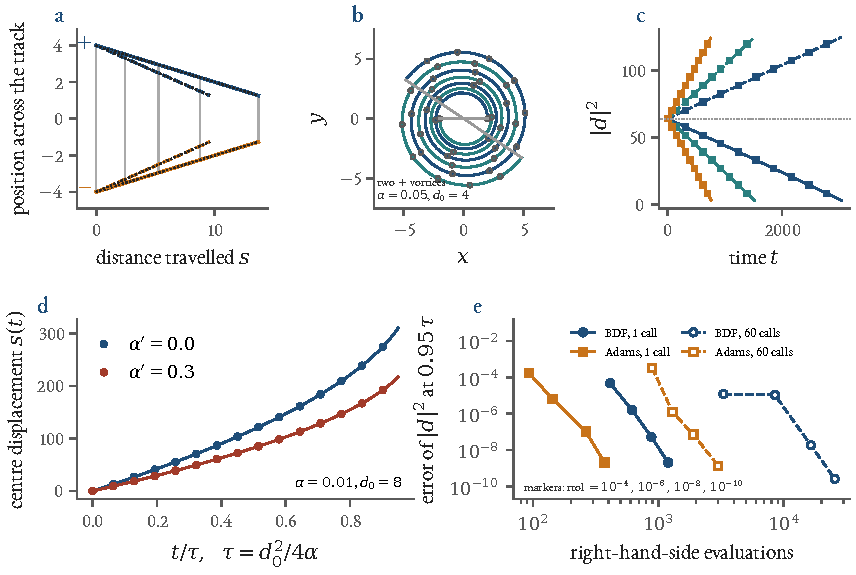
\includegraphics[width=\linewidth]{figures/ch07_dipole.pdf}
\caption[CVODE against the Lean statements on dissipative vortex pairs]{CVODE (\texttt{rusty\_sundials}) against the statements of \cref{ch07:lean}. \textbf{a}~A dipole shrinking and translating: $+$ (blue) and $-$ (orange) vortices in the frame of the track, $\alpha'=0$ (solid) and $0.3$ (dashed),
exact curves dotted, pair axis in grey at five times; $\alpha=0.2$ is ten times a thermal value, chosen so that the funnel is visible. \textbf{b}~Two $+$ vortices spiral apart ($\alpha=0.05$, $d_0=4$, $600$ time units, 3.4 turns);
grey circles: closed form. \textbf{c}~$|\mathbf d|^2$ against time: dipoles (solid) fall with slope $-4\alpha$, same-sign pairs (dashed) rise with $+4\alpha$, for $\alpha=0.005,\,0.01,\,0.02$ (blue, teal, orange); filled markers $\alpha'=0$, open $\alpha'=0.3$.
\textbf{d}~Displacement of the centre of a dipole against the closed form $s=(1-\alpha')(d_0-d)/2\alpha$. \textbf{e}~Work and precision: right-hand-side evaluations against the error of $|\mathbf d|^2$ at $0.95$ of the lifetime ($\alpha=0.01$, $\alpha'=0.1$) for BDF and Adams at $\texttt{rtol}=10^{-4},\dots,10^{-10}$, in one call (filled) and in a chain of $60$ outputs (open).}
\label{ch07:fig-dipole}
\end{figure}


\section{A vortex pair in a thermal field}\label{ch07:field}

\subsection*{The instrument}

The field is the projected Gross--Pitaevskii equation $i\partial_t\psi=\mathcal P[-\tfrac12\nabla^2\psi+g|\psi|^2\psi]$ on a periodic square box of side $L=64$, with $\hbar=m=g=1$ and mean density $n=1$ (healing length $\xi=1$, sound speed $c=1$),
$128\times128$ grid points and a sharp cutoff $|k|\le k_c=\pi$, half the grid wavenumber~\cite{Davis2001,Blakie2008}. The energy is conserved (to $10^{-7}$--$10^{-6}$ over every run of the campaign); nothing is damped and no noise is added. The temperature of a
base state comes from an equipartition thermometer and its normal fraction from the current correlators~\cite{Callens2026a}. The base state of this section is the campaign's $e=0.60$ state: $T=0.115$, that is $T/T_{\rm BKT}=0.14$ with $T_{\rm BKT}(L{=}64)=0.821$ from a heating
ladder, and $\rho_n/\rho=0.027$.

A pair is written into the state by multiplying $\psi$ by the Jacobi-theta phase of the vortex configuration, made single-valued on the torus by a uniform phase gradient, and by the Bernoulli amplitude $[1+|\mathbf v|^2/2]^{-1/2}$ of the imprinted flow. Vortices are found by the
plaquette phase-winding rule that \lean{VortexWinding} proves correct (\cref{ch03}), refined to sub-grid precision, followed by continuity (same sign, nearest detection within $3\xi$) and recorded every time unit. A single pair in a periodic box carries impulse and drives a mean flow, so the
simulations imprint \emph{two antiparallel pairs}, a $+-$ pair at $x=L/4$ and a $-+$ pair at $x=3L/4$ of equal separation $d_0$: zero net charge, dipole moment and impulse, the two pairs travelling in opposite directions.

\begin{rustbox}{two antiparallel pairs in a thermal field (qf-pgpe)}
\begin{lstlisting}[style=py,basicstyle=\ttfamily\footnotesize]
c = np.ascontiguousarray(s.imprint_v2(np.ascontiguousarray(c0), pos, q)); E0 = s.energy(c); t = 0.0; last = pos.copy()
# ...
dp, dq = s.detect(c); dp = np.asarray(dp); dq = np.asarray(dq); cur = np.full_like(last, np.nan)
for i in range(len(q)):
    cand = np.nonzero(dq == q[i])[0]
    if len(cand):
        d = dp[cand] - last[i]; d -= L * np.round(d / L); r = np.hypot(d[:, 0], d[:, 1]); j = int(np.argmin(r))
        if r[j] <= a.r_track:
            cur[i] = dp[cand[j]]
# ...
c = np.ascontiguousarray(s.run(c, 1.0)); t += 1.0
\end{lstlisting}
\nopagebreak[4]\smallskip\noindent\textit{Excerpt of \texttt{book/figures/ch07\_pairrun.py}, as run (\texttt{s} is \texttt{qf\_pgpe.Pgpe(128, 64.0)}, \texttt{c} the projected Fourier amplitudes, \texttt{last} the previous positions). The run was advanced in five chunks of $100$ to $500$ time units, each under the
shared-machine lock, and checkpointed: 928\,s of wall-clock for 1500 time units on one thread, at load average $7$--$18$ on 8 cores.}
\end{rustbox}

\subsection*{The control that caught the first instrument}

An instrument has to be tested where the answer is known. At $T=0$ a pair in a uniform condensate has no excitation to rub against, and the model says its separation must not shrink. The campaign's first known-answer gate did not use this control: it was a single dipole at $T/T_{\rm BKT}\approx0.14$ with the
imprint of the earlier rounds and a biased vortex detector, and it \emph{passed}, narrowly: four fits gave $\alpha=0.0093,\ 0.0062$ ($d_0=8$) and $0.0028,\ 0.0022$ ($d_0=12$), median $0.0045$, inside the window $[0.004,0.045]$ registered from an interpolation of the values published by Shukla, Brachet and Pandit~\cite{Shukla2014}.
That the friction fell with the size of the pair was not predicted, and was noted. The $T=0$ control was run next, and it failed.

\begin{figure}[!tb]\centering
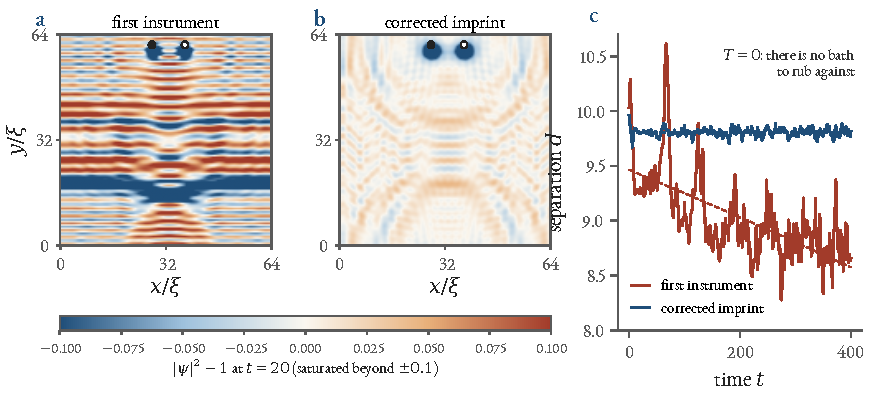
\includegraphics[width=\linewidth]{figures/ch07_imprint.pdf}
\caption[A zero-temperature control of the vortex imprint]{A $T=0$ control. A single pair of separation $10$ is imprinted in a uniform condensate ($L=64$) and $|\psi|^2-1$ is shown $20$ time units later. \textbf{a}~The imprint of the first instrument leaves a phase step along a whole line of the box and a density tail, which become a sheet of sound.
\textbf{b}~The corrected imprint leaves a quiet wake. \textbf{c}~Separation against time over $400$ time units, from the archived tracks of the two gate runs (first attempt: failed; second: passed); dashed, a straight line fitted to $d^2$.}
\label{ch07:fig-imprint}
\end{figure}

\Cref{ch07:fig-imprint} shows why. With the first imprint the pair, which cannot lose energy to a bath that does not exist, closed from $10.03$ to $8.66$ in $400$ time units: an \emph{apparent} friction $\alpha=0.0100$ from the slope of $d^2$, more than the thermal value measured later at $T/T_{\rm BKT}=0.14$ ($0.0062$).
The peak density just after the imprint is $1.084$ against $1.007$ with the corrected one, and at $t=20$ the field momentum is $0.75$ of $2\pi nd$ against $0.96$. Two defects were responsible: the theta-function phase of a single pair is periodic on the torus only if
$\sum_iq_i\mathbf r_i\in L\mathbb Z^2$, otherwise it jumps by $2\pi d/L$ across a boundary and the projection turns the jump into a sheet of sound; and the usual per-vortex amplitude $[r^2/(r^2+2)]^{1/2}$ has a $1/r^2$ tail four times the Bernoulli depletion, whose excess leaves as sound and pushes the vortices (cf.~\cite{Rorai2013}).
With the corrected imprint the pair stays at $9.96\to9.81$ ($|\alpha_{\rm apparent}|<10^{-5}$).

The ledger records the consequence without softening: the pass of the first gate \emph{is withdrawn}, and the stalled single pair that had motivated the hypothesis of \cref{ch07:wind} lost its standing as evidence. The replacement is the corrected instrument at $T=0.115$ with a window fixed in advance: $\alpha_{\rm energy}=0.00705\pm0.00012$ in $[0.0028,0.0112]$.
The lesson is which known answer to ask for first: the $T=0$ control is the cheapest, and the one a theorem makes decisive, since with no bath there is nothing to dissipate into.

\subsection*{The field, and what is measured in it}

\begin{figure}[!tb]\centering
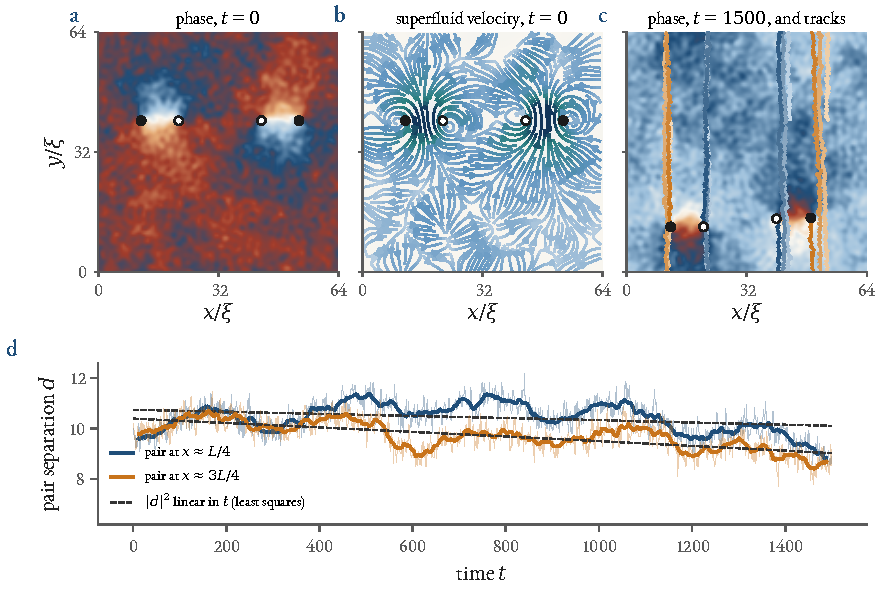
\includegraphics[width=\linewidth]{figures/ch07_fields.pdf}
\caption[Two antiparallel vortex pairs in a thermal projected Gross--Pitaevskii field]{Two antiparallel vortex pairs in a thermal projected-GP field ($T=0.115$, $T/T_{\rm BKT}=0.14$, $L=64$, $d_0=10$), evolved with the Rust engine for 1500 time units (one run, seed 7; relative energy drift $6.8\times10^{-8}$).
\textbf{a}~Phase of $\psi$ just after the imprint; open circles are $+$ vortices, filled circles $-$ vortices. \textbf{b}~The superfluid velocity $\mathrm{Im}(\psi^*\nabla\psi)/|\psi|^2$ coarse-grained over $3\xi$: the jets between the members of each pair and the return flow around them;
the thermal phonons are the faint background. \textbf{c}~Phase at the end of the run with the four tracks (colour: time, drawn on the periodic box). \textbf{d}~Separations of the two pairs against time; dashed, least-squares fits of $d^2$ against $t$.}
\label{ch07:fig-fields}
\end{figure}

\Cref{ch07:fig-fields} shows what the instrument sees. At $t=0$ each pair is a dipole: between its members the superfluid velocity is a jet of speed about $1/d$, the two jets point in opposite directions, and each vortex rides on the jet of its partner. Over 1500 time units the two pairs travel about 2.5 times round the box in opposite directions, at the speeds $0.104$ and $0.111$ (the planar $1/d$ would give about $0.1$). The torus point-vortex model, evaluated at the tracked positions, gives $0.102$ and $0.111$: the measured speed is $1.018$ and $0.998$ of the model's, the regression coefficient $1-\alpha'$ below being $1.007\pm0.006$ (jackknife over eight blocks of the track), so that the centre moves at the model velocity with no sideways force within the errors, as the centre identity of \cref{ch07:lean} says it should. (The planar formula $1/d$ is 6 and 7 per cent below the model for the two pairs: the model adds the periodic images and the second pair.) The separations go from 9.7 to 8.8, between 8.4 and 11.4 along the way: the run reached the planned $t=1500$ with all four vortices tracked throughout. The detected position of a core jitters by $0.31$ per coordinate (the zero-lag offset of the residuals, $c_0=0.20$, for the archived runs of this arm).
A least-squares slope of $d^2$ reads $\alpha=0.0033$ (mean of the two pairs; separately $+0.0022$ and $+0.0044$): to be compared with the estimators below, not trusted over them.

The estimators the programme registered are the energy identity~\eqref{ch07:eq-energy} and a two-coefficient regression: for each tracked vortex the displacement over a lag of $10$ time units is regressed on $\int\mathbf v_{s,i}\,dt$ and $-q_i\!\int\hat{\mathbf z}\times\mathbf v_{s,i}\,dt$, with $\mathbf v_{s,i}$ the torus point-vortex velocity induced by the \emph{other tracked vortices}; the
coefficients are $1-\alpha'$ and $\alpha$, and the mean square of the residuals against lag gives $\eta$. Both are in the Rust extension, \texttt{qf\_pgpe.analyse\_tracks(tracks, 64.0)}, which takes a list of (times, positions, charges) and returns the estimates with block-jackknife errors. It agrees with the Python code of the campaign to $1\times10^{-14}$ (relative) on the eight archived tracks
of this arm (Python: 29\,s; Rust: 1.2\,s, on the loaded machine) and reproduces the campaign's numbers: $\alpha_{\rm energy}=0.00617\pm0.00041$, $\alpha_{\rm regression}=0.00645\pm0.00037$, $1-\alpha'=1.0100\pm0.0015$.

\begin{figure}[!tb]\centering
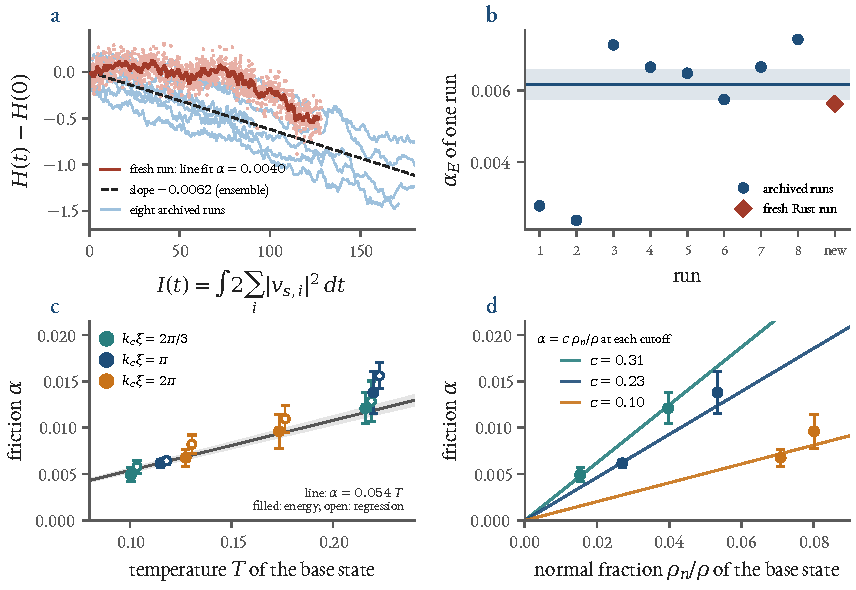
\includegraphics[width=\linewidth]{figures/ch07_friction.pdf}
\caption[The friction in the field]{The friction in the field. \textbf{a}~The energy identity on the tracks: $H(t)-H(0)$ against $I(t)=\int2\sum_i|\mathbf v_{s,i}|^2dt$ falls along a line of slope $-\alpha$ (red: the fresh run, samples and means of $25$ consecutive samples; light blue: the eight archived runs, the same means over the same duration; dashed: the slope of the ensemble).
\textbf{b}~Single-run estimates $\alpha_E$ at $T=0.115$: the eight archived runs and the fresh one, against the ensemble mean and its jackknife error (band). \textbf{c}~The friction of the six arms of the cutoff scan against the temperature of the base state (filled: energy estimator; open, shifted right: regression); the line is
$\alpha=0.054\,T$ (band: one standard error). \textbf{d}~The same data against the normal fraction: within each cutoff the points are proportional to $\rho_n/\rho$, with a coefficient $c$ that changes by a factor $3$ from one cutoff to the next.}
\label{ch07:fig-friction}
\end{figure}

\Cref{ch07:fig-friction}a is the theorem at work, with its caveat. For every run $H(t)$ and $I(t)$ are computed from the tracked positions only, and the identity says that they lie on a line of slope $-\alpha$. The eight archived runs (light blue) do, within the thermal scatter of the detected positions, but with slopes that differ from run to run: over the same
1500 time units their single-run $\alpha_E$ has a mean of $0.0057$ and a standard deviation of $0.0020$, 35 per cent of the mean (panel~b). The fresh run (red) gives $\alpha_E=0.0056$ and $\alpha_R=0.0037$ from the registered estimators (they fit the two halves of every track separately and pool them, so that block-jackknife errors can be given; one straight line through the whole track gives $0.0040$). That puts the run on the ensemble mean (0.02 standard deviations away, number 3 of the nine single runs counted from the lowest).
It is one seed, drawn once and not replaced. The same run analysed at its checkpoint $t=1000$, while the last chunk was waiting for a processor, had given $\alpha_E=-0.0013$ and $\alpha_R=-0.0016$: the estimate of one track moved by $0.0070$ in $500$ time units, and nothing was decided on that interim look.
A pair at this temperature should lose $4\alpha t\approx37$ in $d^2$ over the run, that is, $d$ should fall from $10$ to $7.9$; but the separation of one pair wanders by up to $2.6$ in the $25$-unit means within the run (\cref{ch07:fig-fields}d), so a single track cannot isolate the drift. That is why the campaign used six to eight runs per temperature and quoted jackknife errors over runs; and it is the reason that the identity,
which is exact in the model, is a way of \emph{estimating} $\alpha$ and not a way of seeing it in one track.

\begin{table}[!tb]\centering\small
\begin{tabular}{lcccccc}
\toprule
$T$ & $T/T_{\rm BKT}$ & $\rho_n/\rho$ & runs & $\alpha$ (energy) & $\alpha$ (regression) & $\alpha_{d_0=8}/\alpha_{d_0=12}$\\
\midrule
$0$ & $0$ & $0$ & 1 & $4.1\times10^{-4}$ (floor) & $2.0\times10^{-4}$ & ---\\
$0.115$ & $0.14$ & $0.027$ & $8$ & $0.0062\pm0.0004$ & $0.0064\pm0.0004$ & $0.91$\\
$0.220$ & $0.27$ & $0.053$ & $6$ & $0.0138\pm0.0023$ & $0.0156\pm0.0014$ & $0.76$\\
$0.353^{\dagger}$ & $0.43$ & $0.095$ & $6$ & $0.0205\pm0.0138$ & $0.0242\pm0.0065$ & $1.04$\\
\bottomrule
\end{tabular}
\caption{Friction of a vortex pair in the closed field ($L=64$, $k_c=\pi$; two antiparallel pairs of sizes $8$ and $12$, tracks of up to $2000$ time units), the archived campaign re-analysed with the Rust estimators. Errors are block jackknives over runs.
$^\dagger$A thermal vortex is present in more than $5\%$ of the samples of this base state; the error is large and the base is kept with that flag. The energy estimator is low by the diffusion bias of \cref{ch07:bias}.}
\label{ch07:tab-alpha}
\end{table}

\Cref{ch07:tab-alpha} gives the friction at the three temperatures. The three criteria registered for it passed: the two pair sizes agree (ratios $0.91$, $0.76$, $1.04$, inside the registered $[0.7,1.43]$ at two of three temperatures), $\alpha$ increases with
$T$, and the two estimators agree within $5$, $13$ and $18$ per cent. At $0.14\,T_{\rm BKT}$ the value is a factor two below an interpolation of the values of Shukla, Brachet and Pandit~\cite{Shukla2014}, whose own transition temperature is an estimate; at $0.27$ and $0.43$ no closed-field value existed before, and these lie in the range of the oblate-condensate
measurements~\cite{Moon2015}. One more observation was \emph{not} registered, and is the subject of the next section: $\alpha/(\rho_n/\rho)=0.23,\,0.26,\,0.22$.

\section{Friction follows the temperature, not the normal density}\label{ch07:law}

\subsection*{A kinetic reading, a proportionality, and a prediction}

In the projected field the bath is a finite set of modes $k\in K$ (3208 of them at $k_c=\pi$ in this box). For excitations of occupation $n_k$ and transport cross-section $\sigma_{\rm tr}(k)$ (a length, in two dimensions), a vortex moving slowly through them feels the drag $F=-Dv$ with
$D=\tfrac12\int\frac{d^2k}{(2\pi)^2}(-\partial n/\partial\varepsilon)\,k^2\,c_g\sigma_{\rm tr}$, $c_g=d\varepsilon/dk$, while the Landau normal density of the same gas is $\rho_n=\tfrac12\int\frac{d^2k}{(2\pi)^2}(-\partial n/\partial\varepsilon)\,k^2$: two integrals of the same weight, the first with one extra factor $c_g\sigma_{\rm tr}$.
A force balance on a weakly damped vortex gives $\alpha=D/(\rho_s\kappa)$. The finite sums are what Lean sees: with nonnegative weights $w_k$ and drag factors $f_k=c_g\sigma_{\rm tr}$, $D=\sum_kw_kf_k$ and $\rho_n=\sum_kw_k$, so that $\alpha/(\rho_n/\rho)$ is $\rho/(\rho_s\kappa)$ times the $w$-weighted mean of $f$, and that mean lies between the smallest and the largest $f$ over the bath.

\begin{leanbox}[unbreakable]{FrictionKinetic}
\begin{lstlisting}[style=lean,basicstyle=\ttfamily\footnotesize]
variable {ι : Type*}

/-- The friction coefficient of the kinetic model: `α = D/(ρ_s κ)` with `D = Σ w f`. -/
noncomputable def alpha (K : Finset ι) (w f : ι → ℝ) (ρs κ : ℝ) : ℝ := (∑ k ∈ K, w k * f k) / (ρs * κ)

/-- The Landau normal density of the same bath: `ρ_n = Σ w`. -/
noncomputable def rhoN (K : Finset ι) (w : ι → ℝ) : ℝ := ∑ k ∈ K, w k

theorem coeff_eq_weighted_mean (K : Finset ι) (w f : ι → ℝ) (ρ ρs κ : ℝ) (hρn : rhoN K w ≠ 0) (hρ : ρ ≠ 0) :
    alpha K w f ρs κ / (rhoN K w / ρ) = ρ / (ρs * κ) * ((∑ k ∈ K, w k * f k) / ∑ k ∈ K, w k) := by

theorem weighted_mean_mem_Icc (K : Finset ι) (w f : ι → ℝ) (hw : ∀ k ∈ K, 0 ≤ w k) (hpos : 0 < ∑ k ∈ K, w k)
    (m M : ℝ) (hm : ∀ k ∈ K, m ≤ f k) (hM : ∀ k ∈ K, f k ≤ M) :
    (∑ k ∈ K, w k * f k) / (∑ k ∈ K, w k) ∈ Set.Icc m M := by
\end{lstlisting}
\nopagebreak[4]\smallskip\noindent\textit{Statements only; the proofs are in the module.}
\end{leanbox}

The two theorems are \Lthm{FrictionKinetic}{coeff_eq_weighted_mean} and \Lthm{FrictionKinetic}{weighted_mean_mem_Icc}; for a Rayleigh--Jeans bath with phonon dispersion the weights are equal (\Lthm{FrictionKinetic}{rayleigh_jeans_mean}). Two things follow, and the programme drew only the first. The law $\alpha\propto\rho_n$ is an
\emph{identity} of the kinetic model, for any bath. And its coefficient is not a number about the vortex: it is a mean of $c_g\sigma_{\rm tr}$ \emph{over the modes of the bath}. The module says so itself: ``No claim about the value or the $k$-dependence of $\sigma_{\rm tr}$ is made; that is the measurement.''

At $k_c=\pi$ the measurement gave $\alpha/(\rho_n/\rho)=0.23,\,0.26,\,0.22$ over a factor $3.5$ in $\rho_n$, and the first paper read that coefficient as the mode-averaged transport cross-section of the vortex, $\approx1.4\xi$, ``the geometric size of the core''~\cite{Callens2026a}. That reading assumes that the coefficient belongs to the vortex and not to the bath; the check is to change the bath. The programme registered the test before running it, at two further
cutoffs ($k_c=2\pi/3$ and $2\pi$, same instrument, $T=0$ known answer reproduced at each): FL2, the coefficient differs between the three cutoffs by less than $20\%$, as a property of the vortex should; against a rival, the Born law of long-wavelength phonon scattering extended to the cutoff, which makes it proportional to $k_c$ ($0.67:1:2$).

\subsection*{Both predictions fail}

The coefficient is $0.31\pm0.03$, $0.232\pm0.014$ and $0.102\pm0.011$ at $k_c\xi=2.1,\ 3.1,\ 6.3$ (weighted means over the arms of each cutoff, recomputed here from the six arms): the spread $(\max-\min)/\text{mean}$ is $0.98$ against the registered $0.2$, so FL2 fails; the Born rival fails too ($\chi^2=204$ for $2$ degrees of freedom: the
coefficient \emph{falls} with the cutoff, and the Born law makes it rise); one common coefficient for the six arms fails ($\chi^2=76$ for $5$). Proportionality to $\rho_n$ holds within each cutoff where two temperatures exist, as the identity says it must. The implied mode-averaged cross-section $c\,\kappa\,\rho_s/\rho$ is $1.9\xi$, $1.4\xi$ and $0.59\xi$ (ledger values, each arm's own $\rho_s$): not a property of the vortex.
The ``geometric core size'' reading is \textbf{withdrawn}.

What does not move with the cutoff is the friction itself. \Cref{ch07:fig-friction}c shows the six arms on one line, $\alpha/T=0.0540\pm0.0026$ ($\chi^2=1.28$ for $5$ degrees of freedom, against $76$ for a common $c$), or $0.0598\pm0.0023$ with the regression estimator ($\chi^2=5.15$). In the first paper the three temperatures were taken at one cutoff, where
$\rho_n/\rho$ grows in proportion to $T$, so that a proportionality to either could not be told from the other; the cutoff scan broke the degeneracy (\cref{ch07:fig-friction}c,d). The temperature law was found \emph{after} the data of five arms were read. It was registered, as amendment FL-A1, as a hypothesis, with its prediction for the arm still running fixed in advance: $\alpha=0.0094\pm0.0010$ at
$k_c=2\pi$, $T=0.173$, against $0.0077$ if the friction followed $\rho_n$ with that cutoff's coefficient. The arm gave $0.0096\pm0.0018$: inside the window registered for the temperature law, outside the other. The honest reading is smaller than the verdict: the error is almost twice the one assumed when the window was written, so the ledger puts this arm alone at $0.2\sigma$ from one value and $1.0\sigma$ from the other, and the
discrimination rests on the comparison across cutoffs. The law has been tested over $T=0.10$--$0.22$ and three cutoffs, in one box at one coupling; not above $T=0.22$, where thermal vortices enter.

\subsection*{What transfers, and what does not}

LL-15, the programme's rule, says that an analogy between two systems is not a result: name the property a finding depends on and check that the other system has it. The law $\alpha\propto T$ depends on a property of the \emph{bath}. In a classical field every mode carries the energy $T$, so $n_k=T/\varepsilon_k$ and anything linear in the occupation is linear in $T$; if
$\int^\infty\sigma_{\rm tr}\,dk$ converges (for $k\xi\gg1$ the weight of $D$ makes the integrand $\propto\sigma_{\rm tr}(k)$), the friction is also independent of the cutoff, while $\rho_n$ grows logarithmically with it. Does a quantum gas have the property? We computed Landau's formula $\rho_n=\tfrac12L^{-2}\sum_kk^2(-\partial n/\partial\varepsilon)$ for free Bogoliubov quasiparticles, $\varepsilon_k^2=k^2+k^4/4$, on the actual mode set of each of the six arms (\texttt{figures/ch07\_bath.py}), once with the equipartition occupation $n_k=T/\varepsilon_k$ of the field and once with the Bose occupation $1/(e^{\varepsilon_k/T}-1)$ of a gas at the same temperature. The equipartition sum gives 64--84 per cent of the measured normal fraction of the arm (the rest is interaction); the Bose sum is smaller than the equipartition one by a factor 6 to 48.

So the field does not have it. At $T=0.115$ the equipartition occupation of the mode at the cutoff, $k=\pi$ with $\varepsilon=5.85=51\,T$, is $0.020$ and the Bose occupation is $8\times10^{-23}$; at $k=1$ the ratio is $1.7\times10^{3}$; only at $k\lesssim0.2$, $\varepsilon\approx1.75\,T$, do the two agree within a factor $3$. Of the equipartition Landau sum at $k_c=\pi$, $T=0.115$, only
$0.25\,\%$ comes from modes with $\varepsilon<T$ ($2.2\,\%$ from $\varepsilon<3T$): the normal density of the classical field is carried by modes that a quantum gas at that temperature would not populate, and its normal fraction is about thirty times that of the Bose bath ($0.0227$ against $0.00075$). So the temperature of the classical field is a parameter of the model, which maps onto a physical
temperature only through the cutoff~\cite{Callens2026b}, and the friction law of this section is a law of \emph{this} model; the earlier advice to compare with quantum gases at equal $\rho_n/\rho$ rather than at equal $T/T_c$ is withdrawn in the same sense. What a quantum bath would give, for helium, needs the excitation energies that Godfrin's neutron measurements fix and the cross-section of a vortex for those excitations,
which this programme has not measured. The direct measurement, a monochromatic Bogoliubov wave scattered by one vortex at $T=0$, is the obvious next experiment; it is not in this chapter.


\section{The sideways force and the random kicks}\label{ch07:alphaprime}

\subsection*{A prediction that failed, and a coefficient that is zero}

The registered prediction for $\alpha'$ was the Iordanskii one: a weighted regression of $\hat\alpha'$ on $\rho_n/\rho$ over the temperatures, $T=0$ included, with a slope in $[0.6,1.4]$; ``no transverse force'' was a $2\sigma$ upper bound on the slope below $0.3$. In the frame of the simulation box the values are
\emph{negative}: $\hat\alpha'=-0.0100\pm0.0015,\ -0.0154\pm0.0029,\ -0.0093\pm0.0106$ at the three bases of \cref{ch07:tab-alpha} ($+0.0014$ at $T=0$), a slope of $-0.31\pm0.05$, $18\sigma$ from the Iordanskii window. The registered prediction is \textbf{refuted}, and the rule returns ``no transverse force''.
A negative $\alpha'$ has no theory behind it, though, and it was not left there: two kinematic facts about a compressible pair on a torus, both measured at $T=0$, explain most of it.

First, a single pair carries field momentum $2\pi nd$, which in a periodic box is a mean superfluid velocity $u=2\pi d/L^2$ of the whole fluid, absent from the periodic point-vortex velocity: in a $T=0$ sweep of single pairs the ratio of measured to torus point-vortex speed rises in the box frame from $1.05$ at $d=6$ to $1.46$ at $d=16$ (the saved file \texttt{pair\_speed\_T0.json}; the programme's note quotes $1.06$ and $1.49$), and in the fluid frame, which the ledger reports and which is not re-derived here, the pair moves at the point-vortex speed to
$+1\%$ at $d=6$ and $+0.4\%$ for $d\ge8$ (CLAIM-082). For two antiparallel pairs $|u|\le2\times10^{-3}$ and the pairs move in opposite directions, so the correction is below $0.0002$: decisive for single pairs only. Second, a pair of finite size is a solitary wave of the compressible field, whose speed departs from the point-vortex one (the Jones--Roberts correction) by $+3$--$4\%$ at $d=3$--$4$,
$+1\%$ at $d=6$ and $+0.4\%$ for $d\ge8$. Subtracting this baseline at the pair sizes the fits use gives $\alpha'=-0.0060\pm0.0015,\ -0.0112\pm0.0031,\ -0.0055\pm0.0106$ (CLAIM-082), with an uncertainty of the same order from the mapping between fit weights and pair sizes: \textbf{$\alpha'$ is zero within about $1\%$}, and the Iordanskii values $+2.7\%$, $+5.3\%$, $+9.4\%$ are excluded. The
``vortices move faster than the point-vortex velocity'' of the first analysis was mostly the compressibility of tight pairs at $T=0$. This is a classical field at one cutoff; Shukla, Brachet and Pandit read a nonzero $\alpha'$, without error bars, in the truncated field~\cite{Shukla2014}, and with a different arrangement (antiparallel pairs, the $T=0$ baseline subtracted) we do not adjudicate. In the cutoff scan the box-frame $\hat\alpha'$ stays small and negative ($-0.017$ and
$-0.031$ at $k_c=2\pi/3$, $-0.005$ and $-0.004$ at $2\pi$): reported, unexplained.

\subsection*{The Einstein relation, as an identity}

Take the stochastic pair of \cref{ch07:model}: drift $\mathbf b=-2\alpha\,\mathbf d/|\mathbf d|^2$ on the separation and isotropic noise of diffusion constant $D=2\eta$ (the separation is the difference of two walkers). Its probability current for a density $p$ is $\mathbf J=\mathbf bp-D\nabla p$, and the equilibrium pair gas of the Coulomb-gas picture of the
transition~\cite{KosterlitzThouless1973} has $p\propto|\mathbf d|^{-K}$ with $K=2\pi\rho_s/T$.

\begin{leanbox}{EinsteinRelation}
\begin{lstlisting}[style=lean,basicstyle=\ttfamily\footnotesize]
/-- The pair distribution `|d|^{−K}`, as a function of the two coordinates. -/
noncomputable def p (K x y : ℝ) : ℝ := (x ^ 2 + y ^ 2) ^ (-K / 2)

noncomputable def Jx (α D K x y : ℝ) : ℝ :=
  -2 * α * x / (x ^ 2 + y ^ 2) * p K x y - D * (-K * x / (x ^ 2 + y ^ 2) * p K x y)

theorem zero_flux_iff (α D K : ℝ) :
    (∀ x y : ℝ, x ^ 2 + y ^ 2 ≠ 0 → Jx α D K x y = 0 ∧ Jy α D K x y = 0) ↔ D * K = 2 * α := by

theorem einstein_vortex (α η ρ T : ℝ) (hρ : 0 < ρ) (hT : 0 < T) :
    (∀ x y : ℝ, x ^ 2 + y ^ 2 ≠ 0 → Jx α (2 * η) (2 * π * ρ / T) x y = 0 ∧ Jy α (2 * η) (2 * π * ρ / T) x y = 0)
      ↔ η = α * T / (2 * π * ρ) := by
\end{lstlisting}
\nopagebreak[4]\smallskip\noindent\textit{Statements only; the proofs are in the module.}
\end{leanbox}

The current vanishes at every separation if and only if $DK=2\alpha$; in vortex units the pair gas can be in detailed balance iff $\eta=\alpha T/(2\pi\rho)$, the relation of Mehdi et al.~\cite{Mehdi2023}. Three things the programme measures separately, the shrinking of a pair ($\alpha$), the random walk of its separation ($D$) and the stiffness ($K$), are tied by one identity, and
$R_E=\eta K/\alpha$ is $1$ exactly when the gas can be in equilibrium at that stiffness. The Lean statement adds not the physics, which is Einstein's of 1905, but the fact that the test statistic of the pre-registration is an identity of the model with the equilibrium it presupposes made explicit. That equilibrium is the hypothesis easy to read past: $|\mathbf d|^{-K}$ is an \emph{assumption} about the
state of the gas, and if the bath is not in equilibrium on the time scales sampled, $R_E\neq1$ is not a violation of the identity.

\begin{table}[!tb]\centering\small
\begin{tabular}{lccccc}
\toprule
$T/T_{\rm BKT}$ & $\gamma$ & $\eta$ & $K$ & $R_E$ & quoted\\
\midrule
$0.14$ & $0.71$ & $(3.7\pm0.7)\times10^{-4}$ & $53.2$ & $3.2\pm0.6$ & no \\
$0.27$ & $0.82$ & $(10.8\pm3.5)\times10^{-4}$ & $27.1$ & $2.1\pm0.7$ & yes \\
$0.43$ & $1.28$ & $(18.3\pm3.6)\times10^{-4}$ & $16.1$ & $1.4\pm0.3$ & no \\
\bottomrule
\end{tabular}
\caption{The random kicks: the local exponent $\gamma$ of $\langle|e|^2\rangle-c_0$ against the lag (lags $20$--$400$), the diffusion constant $\eta$ from $\langle|e|^2\rangle=c_0+4\eta\tau$, the stiffness $K=2\pi\rho_s/T$, and $R_E=\eta K/\alpha$ with errors from $\eta$ alone ($\alpha$ held fixed). Rule E2 quotes $\eta$ only where $\gamma\in[0.8,1.2]$.}
\label{ch07:tab-kicks}
\end{table}

\Cref{ch07:tab-kicks} gives the measurement. The diffusion constant is read from the residuals of the regression, $\langle|e|^2\rangle(\tau)=c_0+4\eta\tau$, where the offset $c_0\approx0.2$--$1.2$ is the thermal jitter of the detected cores; at $T=0$ the residual is bounded at $0.005$. Rule E2, fixed before the analysis, quotes $\eta$ only where the local exponent on lags $20$--$400$ lies in $[0.8,1.2]$: that
admits one temperature of three, $T/T_{\rm BKT}=0.27$, where $R_E=2.1\pm0.7$; the two unquoted temperatures would give $3.2$ and $1.4$. The decision rule needed two admitted temperatures: \textbf{by the rule the Einstein relation is undecided}. Informally, and against the rule, the vortex diffuses at about $1.4$ to $3$ times the Einstein value, the excess falling with temperature: far from
the hundredfold surplus that Neely et al.\ measure in a trap with vibrating walls~\cite{Neely2024}, and not cleanly one. A closed field has no walls to blame. (At $T/T_{\rm BKT}=0.43$ the error of $\alpha$ is $67\%$ and would dominate the error of $R_E$.)

The sub-diffusive exponent at the lowest temperature, $0.71$, invites a reading as a regular island: bounded quasi-periodic motion about the point-vortex trajectory. Lean makes the logic of the test precise: a finite sum of cosines has increments bounded by twice the sum of its amplitudes, so every mean of squared increments is at most $4(\sum_k|a_k|)^2$ at any lag
(\Lthm{QuasiPeriodicBound}{msd_bound}), and \Lthm{QuasiPeriodicBound}{not_qp_of_msd_large} turns this into a refutation, whatever the frequencies and phases. The test is one-sided: growth refutes an island, a plateau never proves one. On lags $\ge100$ the exponents at the two cooler temperatures are $1.24$ and $1.10$, which is growth: the sub-diffusion is a short-lag regime of the jitter, not an island.

\section{The wind that was not}\label{ch07:wind}

The impulse $2\pi\rho_sd$ of a shrinking pair has to go somewhere. In a periodic box it goes into the phonons, which drift at $u=2\pi\rho_s(d_0-d)/(\rho_nL^2)$ along the pair, and friction, which acts on the velocity of the vortex relative to the normal fluid, is reduced: $\dot d=-2\alpha\,(1/d-u)$. This is the programme's hypothesis~W, and Lean has a theorem for it.

\begin{leanbox}{DissipativeVortexDynamics}
\begin{lstlisting}[style=lean,basicstyle=\ttfamily\footnotesize]
theorem wind_stall {a b c : ℝ} (ha : 0 < a) (hab : a < b) (hc : 0 < c) (d : ℝ → ℝ)
    (hd : ∀ t, HasDerivAt d (-c * (d t - a) * (d t - b) / d t) t) (h0 : b ≤ d 0) :
    ∀ t, 0 ≤ t → b ≤ d t := by

example {a b c : ℝ} (hab : a < b) :
    (∀ t : ℝ, HasDerivAt (fun _ : ℝ => a) (-c * (a - a) * (a - b) / a) t) ∧ ¬ (b ≤ a) := by
  refine ⟨fun t => ?_, not_le.mpr hab⟩
  simpa using hasDerivAt_const t a
\end{lstlisting}
\nopagebreak[4]\smallskip\noindent\textit{The second statement is the module's negative control: the hypothesis $b\le d(0)$ cannot be dropped. The first is proved by a ``fence'' argument: a solution that went below $b$ would have to cross a level $b-\varepsilon$ with positive derivative, which the sign of the drive forbids.}
\end{leanbox}

With $a+b=d_0$ and $ab=1/w$, $w=2\pi\rho_s/(\rho_nL^2)$, the wind equation is $\dot d=-2\alpha w(d-a)(d-b)/d$, and when $wd_0^2>4$ it has two positive zeros: a pair starting at or above $b$ never falls below it. The library states the identification of the two forms in a comment; the book's new module makes it a theorem and states the stall for the equation as derived.

\begin{leanbox}[unbreakable]{Ch07\_DissipativePairs (new, not in the library)}
\begin{lstlisting}[style=lean,basicstyle=\ttfamily\footnotesize]
theorem wind_stall_at_b {α w d0 : ℝ} (hα : 0 < α) (hw : 0 < w) (hd0 : 0 < d0) (h4 : 4 < w * d0 ^ 2)
    (d : ℝ → ℝ) (hd : ∀ t, HasDerivAt d (-(2 * α) * (1 / d t - w * (d0 - d t))) t)
    (h0 : stallPoint w d0 ≤ d 0) : ∀ t, 0 ≤ t → stallPoint w d0 ≤ d t := by
\end{lstlisting}
\nopagebreak[4]\smallskip\noindent\textit{\texttt{stallPoint w d0} is $[d_0+\sqrt{d_0^2-4/w}]/2$. The module also proves that the roots are real, ordered and positive with $a+b=d_0$, $ab=1/w$, that for $wd_0^2<4$ the right-hand side has no zero, and a negative control (the hypothesis on the starting point cannot be dropped); all with the three standard axioms.}
\end{leanbox}

For the box of this chapter ($L=64$, $\rho_n/\rho=0.027$) and $d_0=12$: $w=0.055$, $wd_0^2=7.9>4$, and in the plane formula, which neglects the torus's image forces (with them the paper estimates nearer $9$), the stall point is $b=10.2$ (the lower root is $a=1.8$), approached exponentially at the linearised rate $\lambda=2\alpha w(b-a)/b=5.6\times10^{-4}$, a time constant of about
$1800$ time units, with the measured $\alpha=0.0062$ (CVODE, \cref{ch07:fig-failures}a). A pair of $d_0=8$ should not stall ($wd_0^2=3.5<4$). Two single pairs of $d_0\approx12$ at $T=0.115$, run for $4000$ time units, do not annihilate, while the zero-impulse pairs of the same temperature shrink steadily: the four pairs of the two archived runs with $d_0=10$ go from $9.4$--$10.1$ to $7.3$--$8.4$ in $1500$ time units. In the archived data one
pair falls from $11.7$ to $8.8$ by $t\approx1800$ and then wanders between $8.8$ and $10.2$ (the late slope of $d^2$ is $4\%$ of the early one); the other falls to about $9.8$ and re-expands to $11.3$, back toward the stall point, so that by the letter of the registered criterion (late slope below $25\%$ of the early one) it does not stall, though in
substance it stops shrinking. The momentum of the modes with $|k|>1$ follows the impulse shed by the pair, with regression slopes $0.69$ and $0.51$ against the registered window $[0.5,1.2]$ ($0.82$ after the $25$-unit running means of \cref{ch07:fig-failures}b, which remove the attenuation caused by the jitter of the detected separation), and falls back when the pair re-expands. So far hypothesis~W is
supported; metastable counterflow states exist in the Fourier-truncated Gross--Pitaevskii equation~\cite{KrstulovicBrachet2011}, and here the counterflow would be generated by the pair itself.

\begin{figure}[!tb]\centering
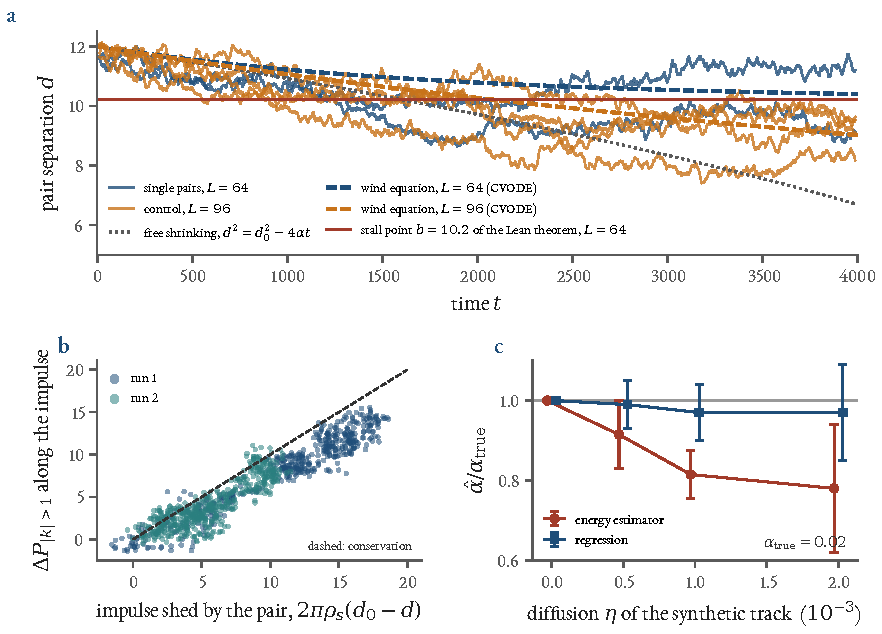
\includegraphics[width=\linewidth]{figures/ch07_failures.pdf}
\caption[Two theorems that were true and did not describe what they were applied to]{Two theorems that were true and did not describe what they were applied to. \textbf{a}~Separation of single pairs at $L=64$ (blue, two runs) and in the $L=96$ control (orange, four runs), $25$-unit running means, against the wind equation integrated with CVODE with the measured $\alpha=0.0062$ and no free parameter (thick dashed), free shrinking (dotted)
and the stall point $b$ of the Lean theorem (red). \textbf{b}~The wind seen directly: momentum of the phonon band $|k|>1$ projected on the initial impulse against the impulse shed by the pair, for the two $L=64$ runs; dashed, conservation of momentum between the pair and the phonons. \textbf{c}~The energy estimator of $\alpha$ on synthetic tracks of known $\alpha=0.02$ against the
diffusion $\eta$ of the track: exact at $\eta=0$ (the theorem), biased low when $\eta>0$; the regression estimator is not.}
\label{ch07:fig-failures}
\end{figure}

Then the control that the programme had registered as decisive was run. In an $L=96$ box at the same temperature ($\rho_n/\rho=0.029$) the same pair has $wd_0^2=3.2<4$: the equation has no zero (\Lthm{DissipativePairs}{wind_no_zero}), the box criterion $\rho_nL^2/(2\pi\rho_s)=44.3$ exceeds $d_0^2/4=36$, and no stall is predicted. A pair that keeps shrinking supports the mechanism; a pair that stalls near the $L=64$
separation refutes it. With a tie-break of two further runs written in advance, the four runs ended at $d=9.3,\ 9.6,\ 8.3,\ 9.5$ (wind equation: $8.0$--$8.9$; free shrinking: $5.3$--$6.5$), and the late shrinking rate was $0$, $10$ and $37\%$ of the early one in runs 2--4, where the mechanism predicted about $50\%$. Only one of four meets the no-stall criterion, and the rule (at most one: refuted) gives the verdict:
\textbf{W2 is refuted; the pairs stall at $L=96$ as at $L=64$, the stall is not the box's, and the explanation by the phonon wind of a closed box is withdrawn.} The parameter-free wind curve of \cref{ch07:fig-failures}a shows that a drift of the normal component is \emph{consistent} with the data (all six pairs end within 0.2--1.5 of the curve of their box, and 1.6 to 4.6 above free shrinking); consistent is not causal. The observation is kept (a reproducible, bath-driven stall
of a single pair at low temperature, with a $1/f^{0.5}$ separation spectrum), the explanation is not, and the graded test that could separate a residual wind from the real cause, a stall map in $L$, $d_0$ and $T$, is registered and has not been run. Every friction measurement on a single pair in a closed box at low temperature is affected, which is why the production runs use the zero-impulse geometry.

This is a clean example of what a proof assistant does and does not do. Lean certified the \emph{implication}: if the pair obeys the wind equation it cannot fall below $b$, and for $L=96$ the equation has no zero. The experiment tested the \emph{premise}, that the equation describes the pair, and refuted it. Nothing in the kernel could have said so.

\section{An estimator that was exact, and was not}\label{ch07:bias}

A second implementation is an instrument. The registered estimators were ported to Rust (crate \texttt{qf-pgpe}, module \texttt{transport}), first for speed, and the port agrees with the Python code on real tracks to $1\times10^{-14}$ (\cref{ch07:field}). Run on the registered synthetic gate G0 (known $\alpha=0.02$, $\alpha'=0.10$, $\eta=2\times10^{-3}$, eight tracks of $2000$ time units) over \emph{many seeds}, it showed what the single seed of
the gate had not.

With no diffusion the energy estimator returns the true value, exactly. With diffusion it is low, by $8.5$, $18.5$ and $22\%$ at $\eta=5\times10^{-4}$, $10^{-3}$, $2\times10^{-3}$, while the regression estimator is low by only $1$ to $3\%$ (\cref{ch07:fig-failures}c). The means over 8 seeds of eight tracks each are $0.0183\pm0.0017$, $0.0163\pm0.0012$, $0.0156\pm0.0032$ for the energy estimator and $0.0198\pm0.0012$, $0.0194\pm0.0014$, $0.0194\pm0.0024$ for the regression estimator, for a true $\alpha=0.02$ and no detection noise (Rust example \texttt{g0\_scan --eta-scan} of \texttt{qf-pgpe}, run for this chapter); the ledger records the bias as independent of the detection noise (CLAIM-098). The gate's criterion (energy estimator within $15\%$) passes on $2$ of $12$ seeds (CLAIM-098); the registered gate had
passed on one lucky seed. In the real arms the regression estimator exceeds the energy one by $5$ to $21\%$, in exactly this direction.

Why did the theorem not warn us? Because it is not about this. Its hypothesis is \texttt{hr}: the path has a derivative at every instant and obeys the flow (\Lthm{DissipativeVortexDynamics}{energy_dissipation}). A diffusing vortex has no derivative; the identity belongs to the \emph{deterministic} model, and the data are not a path of that model. The cause of the bias is not proven (the programme's note suspects that the stochastic part of $H(t)$ is
correlated with the cumulative regressor $\int2S\,dt$, which depends on the same noisy path); what is proven is that the identity applies where its hypothesis holds, and there it is exact ($\alpha_{\rm energy}=0.0200$ at $\eta=0$). This is LL-15 applied to the programme's own tool: a conclusion travels with its preconditions or not at all. No registered verdict changes (they compare arms with the same estimator), but the absolute $\alpha$ of \cref{ch07:tab-alpha}
are low by about $5$--$20\%$ ($0.0062$, $0.014$, $0.02$ become $0.0064$, $0.0156$, $0.0242$ with the regression estimator, \cref{ch07:tab-alpha}), the temperature law reads $0.060\,T$ rather than $0.054\,T$, and the gate's energy criterion is not a reliable known answer; the regression criterion is.

\section{What this chapter establishes, and what it does not}\label{ch07:honest}

\begin{honestbox}
\textbf{Proved in Lean (standard axioms only; checked on 2026-10-09).} The energy identity for any flow of the form~\eqref{ch07:eq-flow}; for the plane dipole, the law $|\mathbf d|^2=|\mathbf d_0|^2-4\alpha t$ and the centre velocity $(1-\alpha')/|\mathbf d|$, and, in the book's new module, the law $+4\alpha t$ of the same-sign pair; the zero-current characterisation $DK=2\alpha$; the kinetic identity for $\alpha/(\rho_n/\rho)$; the stall of the wind equation and, new, its stall at the root $b$; the bound on quasi-periodic mean-square displacements (\cref{ch07:lean,ch07:law,ch07:alphaprime,ch07:wind}). These are statements about \emph{models}, elementary and not new (the new theorems are in \texttt{book/lean/}, not in the library), and none is a statement of Godfrin's papers.

\textbf{Simulated, in a classical projected field (one box, $mg=1$, cutoffs $2\pi/3$, $\pi$, $2\pi$, $T<0.45\,T_{\rm BKT}$).} $\alpha=0.0062(4)$, $0.014(2)$, $0.02(1)$ at $T/T_{\rm BKT}=0.14$, $0.27$, $0.43$ by two estimators, the energy one low by $5$--$20\%$; $\alpha\simeq0.054\,T$ (energy) or $0.060\,T$ (regression) over three cutoffs; $\alpha'=0$ within about $1\%$ once the $T=0$ kinematics of a compressible pair on a torus are
accounted for; the diffusion $1.4$--$3$ times the Einstein value where it can be read; a bath-driven stall of a single pair; one fresh run of $1500$ time units, one seed, inside the scatter of single runs. CVODE reproduces the exact pair laws to $3\times10^{-8}$ (dipole) and $10^{-5}$ (rotating pair).

\textbf{Analogy only, not established.} Anything about helium, atomic gases, or the fluid whose excitations Godfrin measured: the classical-field bath is not a Bose bath (\cref{ch07:law}), the temperature of the field is a parameter of the model, and $\sigma_{\rm tr}(k)$ of a vortex has not been measured here. The Einstein relation is undecided by the registered rule.

\textbf{Failed, withdrawn or corrected.} The first known-answer gate passed on a defective imprint and is withdrawn (CLAIM-075). The reading $\alpha\propto\rho_n$ with a vortex-owned coefficient and the ``geometric core size'' $1.4\xi$ are withdrawn: the coefficient depends on the cutoff, and the registered predictions of FL2 and of the Born law failed. The registered Iordanskii-like prediction for $\alpha'$ is refuted at $18\sigma$. The phonon-wind mechanism is
refuted by the $L=96$ control while its Lean theorem stays true. The energy estimator is biased low by the diffusion, which no theorem was about. The temperature law was formulated after the data of five arms were read and is confirmed, by the registered window, on a sixth arm whose error is larger than was assumed.
\end{honestbox}

\section{Exercises}

\paragraph{Exercise 1.} Show that two vortices of the \emph{same} sign obey $|\mathbf d|^2=|\mathbf d_0|^2+4\alpha t$ and rotate with angular velocity $2(1-\alpha')/|\mathbf d|^2$ about their fixed centre, and find how long a pair with $d_0=4\xi$ and $\alpha=0.02$ takes to double its separation. Then reproduce panel~b of \cref{ch07:fig-dipole}: the listing of \cref{ch07:cvode} needs only a new right-hand side, for two vortices of the same sign.
\emph{Hint.} With $\mathbf d=\mathbf p_1-\mathbf p_2$ the velocities induced at the two vortices are $\pm\hat{\mathbf z}\times\mathbf d/|\mathbf d|^2$; the radial component of $\dot{\mathbf d}$ is $2\alpha/d$, so $d\,\dot d=2\alpha$; the answer to the first question is $3d_0^2/(4\alpha)=600$.

\paragraph{Exercise 2.} Generate synthetic dipole tracks with the Langevin generator of the repository (\texttt{exploration/pgpe/transport\_estimators.py}, function \texttt{langevin}) for $\alpha=0.02$ and $\eta=0$, then $\eta=10^{-3}$, and apply the energy and the regression estimators through \texttt{qf\_pgpe.analyse\_tracks}. Explain, from the hypotheses of \Lthm{DissipativeVortexDynamics}{energy_dissipation}, why the first case must be exact and why
the second need not be. \emph{Hint.} Look at \texttt{hr}: what regularity does a Brownian path have? Expect $\alpha_{\rm energy}\approx0.016$ at $\eta=10^{-3}$ over eight tracks of $2000$ time units.

\paragraph{Exercise 3.} (LL-15.) For $\varepsilon_k=\sqrt{k^2+k^4/4}$ at $T=0.115$ compute $n_{\rm RJ}/n_{\rm Bose}$, with $n_{\rm RJ}=T/\varepsilon_k$ and $n_{\rm Bose}=1/(e^{\varepsilon_k/T}-1)$, at $k=0.2,\,1,\,\pi$. Then compute the fraction of the equipartition Landau sum $\tfrac12L^{-2}\sum_kk^2T/\varepsilon_k^2$ carried by modes with $\varepsilon<T$, on the $3208$ modes of the disk $|k|\le\pi$,
$L=64$. Which statements of \cref{ch07:law} depend on the equipartition occupation, and which would survive in a Bose bath? \emph{Hint.} The first part is three lines of code; the second is a fraction of a per cent.

\section{Notes and further reading}

The programme's two papers on the subject are \cite{Callens2026a}, on friction, the transverse coefficient, the diffusion and the stall of a single pair (Zenodo, version~2.2, October 2026, \texttt{doi:10.5281/\allowbreak zenodo.23262143}), and \cite{Callens2026b}, on the cutoff scan and the temperature law (\texttt{doi:10.5281/\allowbreak zenodo.23262132}); the engine is in \cite{Callens2026sw}, the Lean library in \cite{Callens2026lib}. The static half of the first paper, the box-scale pair, equilibration and the polarisability
of the pair gas, bears on the Kosterlitz--Thouless side of \cref{ch06} and is not treated here. For mutual friction in helium start with Donnelly's book~\cite{Donnelly1991} and the review of Sergeev~\cite{Sergeev2023}; for measurements in atomic gases, \cite{Moon2015} and \cite{Neely2024}, and, in a Fermi superfluid, where the friction and the vortex Hall angle were measured, \cite{Grani2025}; for the diffusion, \cite{Mehdi2023}, and for the stochastic point-vortex model as used
for helium films, \cite{AHNS1980}; for the transverse force, \cite{ThoulessAoNiu1996}, \cite{Iordanskii1964} and \cite{Sonin1997}. The point-vortex flow on the torus is in \cite{WeissMcWilliams1991}, and the integrability of few-vortex flows in the survey~\cite{ModinViviani2021}.
\widowpenalty=\chsevenwp\relax\clubpenalty=\chsevencp\relax
\flushbottom
}
\IfCh{ch13}{\input{chapters/ch13}}
\IfCh{ch09}{\chapter{Flow Past an Obstacle: Reproducing a Published Experiment}\label{ch09}
% generated by book/figures/ch09_texnumbers.py from ch09_numbers.json -- do not edit.  Each macro is math-mode material: write $\cnineForceTen$.
% macros are prefixed cnine to stay clear of the other chapters' names.
\newcommand{\cnineForceTc}{1.1\times10^{-6}}
\newcommand{\cnineForceLtOne}{4.0\times10^{-6}}
\newcommand{\cnineForceFive}{1.4\times10^{-4}}
\newcommand{\cnineForceTen}{2.2\times10^{-4}}
\newcommand{\cnineForceTwenty}{7.9\times10^{-3}}
\newcommand{\cnineForceThirty}{1.7\times10^{-2}}
\newcommand{\cnineForceForty}{1.7\times10^{-2}}
\newcommand{\cnineForceFifty}{1.6\times10^{-2}}
\newcommand{\cnineForceMax}{8.94}
\newcommand{\cnineForceMaxT}{47.8}
\newcommand{\cnineForceMaxTen}{5.45}
\newcommand{\cnineForceOverallPct}{0.19}
\newcommand{\cnineForceOverall}{1.68\times10^{-2}}
\newcommand{\cnineForceRelTen}{4\times10^{-5}}
\newcommand{\cnineForceRelTenTwo}{4.0\times10^{-5}}
\newcommand{\cnineForceRelTc}{6\times10^{-6}}
\newcommand{\cnineForceGrowth}{36}
\newcommand{\cninePlateauMean}{1.6\times10^{-2}}
\newcommand{\cninePlateauMin}{1.5\times10^{-2}}
\newcommand{\cninePlateauMax}{1.7\times10^{-2}}
\newcommand{\cnineZeroCross}{10.7}
\newcommand{\cninePlateauFracAtBirth}{82}
\newcommand{\cnineDragAtBirth}{7.1}
\newcommand{\cninedFatFourteen}{1.3\times10^{-3}}
\newcommand{\cninedFatTwenty}{8.0\times10^{-3}}
\newcommand{\cninedFatTwentyFour}{1.3\times10^{-2}}
\newcommand{\cninedFatTwentyEight}{1.6\times10^{-2}}
\newcommand{\cninedFatFifty}{1.5\times10^{-2}}
\newcommand{\cnineShiftTwenty}{0.12}
\newcommand{\cnineShiftThirty}{0.17}
\newcommand{\cnineShiftForty}{0.50}
\newcommand{\cnineShiftResTwenty}{4}
\newcommand{\cnineShiftResThirty}{26}
\newcommand{\cnineShiftResForty}{71}
\newcommand{\cnineLiftMax}{3.5\times10^{-4}}
\newcommand{\cnineLiftRatio}{4\times10^{-5}}
\newcommand{\cnineLiftRelMin}{0.4}
\newcommand{\cnineLiftRelMax}{3.6}
\newcommand{\cnineLiftZero}{3\times10^{-6}}
\newcommand{\cninePsiTen}{2.2\times10^{-4}}
\newcommand{\cninePsiGaugeTen}{2.1\times10^{-4}}
\newcommand{\cnineDensTen}{2.4\times10^{-4}}
\newcommand{\cnineNearShareTen}{11}
\newcommand{\cninePsiTwenty}{5.8\times10^{-4}}
\newcommand{\cninePsiGaugeTwenty}{4.8\times10^{-4}}
\newcommand{\cnineDensTwenty}{2.0\times10^{-4}}
\newcommand{\cnineNearShareTwenty}{10}
\newcommand{\cninePsiThirty}{1.3\times10^{-3}}
\newcommand{\cninePsiGaugeThirty}{1.0\times10^{-3}}
\newcommand{\cnineDensThirty}{2.0\times10^{-4}}
\newcommand{\cnineNearShareThirty}{39}
\newcommand{\cninePsiForty}{2.5\times10^{-3}}
\newcommand{\cninePsiGaugeForty}{1.9\times10^{-3}}
\newcommand{\cnineDensForty}{2.8\times10^{-4}}
\newcommand{\cnineNearShareForty}{72}
\newcommand{\cninePsiFifty}{4.1\times10^{-3}}
\newcommand{\cninePsiGaugeFifty}{3.3\times10^{-3}}
\newcommand{\cnineDensFifty}{4.0\times10^{-4}}
\newcommand{\cnineNearShareFifty}{80}
\newcommand{\cnineDensRmsMin}{2\times10^{-4}}
\newcommand{\cnineDensRmsMax}{4\times10^{-4}}
\newcommand{\cnineMaxDpsiFifty}{0.045}
\newcommand{\cnineMaxDnFifty}{0.0205}
\newcommand{\cnineGlobalPhaseFifty}{2.5\times10^{-3}}
\newcommand{\cninePaperVc}{0.18}
\newcommand{\cninePaperVth}{0.33}
\newcommand{\cninePaperRes}{2}
\newcommand{\cninePaperTLo}{2000}
\newcommand{\cninePaperTHi}{10000}
\newcommand{\cninePaperWx}{25}
\newcommand{\cninePaperWy}{20}
\newcommand{\cninePaperD}{3}
\newcommand{\cnineProdSteps}{5000}
\newcommand{\cnineProdWall}{2741}
\newcommand{\cnineProdWallMin}{46}
\newcommand{\cnineGammaCentre}{2.4\times10^{-6}}
\newcommand{\cnineGammaDisc}{1.7\times10^{-5}}
\newcommand{\cnineGammaOne}{1.39\times10^{-5}}
\newcommand{\cnineStopThr}{2\times10^{-5}}
\newcommand{\cnineEps}{5\times10^{-4}}
\newcommand{\cnineInitDouble}{2.8\times10^{-8}}
\newcommand{\cnineInitNoise}{4.1\times10^{-4}}
\newcommand{\cnineInitDiffPct}{10.0}
\newcommand{\cnineInitDiffN}{50\,077}
\newcommand{\cnineInitN}{500\,000}
\newcommand{\cnineInitRounded}{3\times10^{-18}}
\newcommand{\cnineOvershoot}{0.00275}
\newcommand{\cnineOvershootHalf}{0.001375}
\newcommand{\cnineSumV}{0.03025}
\newcommand{\cnineIntV}{0.0275}
\newcommand{\cnineRampOffset}{3.5\times10^{-3}}
\newcommand{\cnineRampOffsetHalf}{1.75\times10^{-3}}
\newcommand{\cnineSens}{1.27}
\newcommand{\cnineSensB}{1.2713}
\newcommand{\cnineSensA}{1.2709}
\newcommand{\cnineOwnTemporal}{3.3\times10^{-10}}
\newcommand{\cnineStageMin}{2.7\times10^{-3}}
\newcommand{\cnineStageMax}{3.5\times10^{-3}}
\newcommand{\cnineEqualCounts}{9}
\newcommand{\cnineCensusHeader}{5 & 10 & 15 & 20 & 25 & 30 & 35 & 40 & 45 & 50}
\newcommand{\cnineMatchThirty}{2}
\newcommand{\cnineMatchForty}{14}
\newcommand{\cnineMatchFiftyIdent}{9}
\newcommand{\cnineMatchFiftyClose}{1}
\newcommand{\cnineMatchTotalIdent}{25}
\newcommand{\cnineMatchTotal}{26}
\newcommand{\cnineWindN}{16}
\newcommand{\cnineWindDev}{3\times10^{-16}}
\newcommand{\cnineEdgeMax}{0.9993}
\newcommand{\cnineEdgeMargin}{0.07}
\newcommand{\cnineLoopDiffMax}{0.57}
\newcommand{\cnineLoopDiffThirty}{0.24}
\newcommand{\cnineMarginalInt}{0.951}
\newcommand{\cnineMarginalX}{82.5}
\newcommand{\cnineMarginalY}{4.0}
\newcommand{\cnineMarginalAbove}{5.7}
\newcommand{\cnineAsymZero}{5.7\times10^{-4}}
\newcommand{\cnineAsymRefFifty}{1.4\times10^{-4}}
\newcommand{\cnineAsymOursFifty}{1.8\times10^{-4}}
\newcommand{\cnineAsymOursFive}{3.9\times10^{-4}}
\newcommand{\cnineAsymRefTen}{2.2\times10^{-4}}
\newcommand{\cnineAsymOursTen}{3.5\times10^{-4}}
\newcommand{\cnineSupAreaOursFive}{192}
\newcommand{\cnineSupMOursFive}{1.85}
\newcommand{\cnineSupWidthOursFive}{16.5}
\newcommand{\cnineSupAreaOursTen}{254}
\newcommand{\cnineSupMOursTen}{2.22}
\newcommand{\cnineSupWidthOursTen}{20.5}
\newcommand{\cnineSupAreaOursFifteen}{321}
\newcommand{\cnineSupMOursFifteen}{2.84}
\newcommand{\cnineSupWidthOursFifteen}{23.5}
\newcommand{\cnineSupAreaOursTwenty}{378}
\newcommand{\cnineSupMOursTwenty}{5.38}
\newcommand{\cnineSupWidthOursTwenty}{26.5}
\newcommand{\cnineSupAreaRefTen}{253}
\newcommand{\cnineSupMRefTen}{2.21}
\newcommand{\cnineSupWidthRefTen}{20.5}
\newcommand{\cnineSupAreaRefTwenty}{380}
\newcommand{\cnineSupMRefTwenty}{5.42}
\newcommand{\cnineSupWidthRefTwenty}{26.5}
\newcommand{\cnineSupAreaOursTwentyP}{378.0}
\newcommand{\cnineSupAreaRefTwentyP}{379.5}
\newcommand{\cnineSupXminOursTwenty}{86.0}
\newcommand{\cnineSupXmaxOursTwenty}{102.5}
\newcommand{\cnineSupYhalfOursTwenty}{13}
\newcommand{\cnineSupXMmax}{89}
\newcommand{\cnineAxisNcentre}{0.25}
\newcommand{\cnineAxisUcentre}{0.70}
\newcommand{\cnineAxisMcentre}{1.40}
\newcommand{\cnineAxisJcentre}{0.17}
\newcommand{\cnineAxisJratio}{32}
\newcommand{\cnineAxisNmin}{0.086}
\newcommand{\cnineAxisSpeedMax}{1.58}
\newcommand{\cnineAxisMaxM}{5.4}
\newcommand{\cnineAxisXmin}{89}
\newcommand{\cnineAxisSupLo}{86.5}
\newcommand{\cnineAxisSupHi}{102.5}
\newcommand{\cnineUcFar}{0.876}
\newcommand{\cnineUcCentre}{0.409}
\newcommand{\cnineSqrtOneMinusV}{0.32}
\newcommand{\cnineBernB}{1.1513}
\newcommand{\cnineThrAreaOursFive}{201}
\newcommand{\cnineThrInOursFive}{84}
\newcommand{\cnineMachAreaNearOursFive}{192}
\newcommand{\cnineThrAreaOursTen}{289}
\newcommand{\cnineThrInOursTen}{88}
\newcommand{\cnineMachAreaNearOursTen}{254}
\newcommand{\cnineThrAreaOursFifteen}{379}
\newcommand{\cnineThrInOursFifteen}{95}
\newcommand{\cnineMachAreaNearOursFifteen}{321}
\newcommand{\cnineThrAreaOursTwenty}{450}
\newcommand{\cnineThrInOursTwenty}{99}
\newcommand{\cnineMachAreaNearOursTwenty}{378}
\newcommand{\cnineThrExcessOursTwenty}{19}
\newcommand{\cnineThrExcessOursFive}{5}
\newcommand{\cnineNBernCentre}{0.007}
\newcommand{\cnineNMeasCentre}{0.249}
\newcommand{\cnineBirthBefore}{24.2}
\newcommand{\cnineBirthAfter}{24.3}
\newcommand{\cnineBirthNmin}{9\times10^{-5}}
\newcommand{\cnineBirthNminAfter}{2.7\times10^{-4}}
\newcommand{\cnineBirthX}{86.75}
\newcommand{\cnineBirthY}{0.25}
\newcommand{\cnineBirthDist}{13.25}
\newcommand{\cnineBirthSep}{0.5}
\newcommand{\cnineBirthSepLate}{2.5}
\newcommand{\cnineBirthEdge}{0.998}
\newcommand{\cnineContRel}{1.2\times10^{-15}}
\newcommand{\cnineNminTwenty}{0.086}
\newcommand{\cnineNminTwentyThree}{9.1\times10^{-3}}
\newcommand{\cnineEdgeTwentyFour}{0.78}
\newcommand{\cnineEdgeTwentyFourTwo}{0.61}
\newcommand{\cnineBirthSupLo}{86.0}
\newcommand{\cnineBirthSupHi}{102.0}
\newcommand{\cnineBernCorr}{0.99999}
\newcommand{\cnineBernOneMinus}{7\times10^{-6}}
\newcommand{\cnineBernMaxDiff}{4.2\times10^{-3}}
\newcommand{\cnineBernRms}{0.12}
\newcommand{\cnineBernRspan}{0.6}
\newcommand{\cnineBernRlo}{-0.21}
\newcommand{\cnineBernRhi}{0.39}
\newcommand{\cnineBernQsmall}{0.028}
\newcommand{\cnineBernQmin}{-0.36}
\newcommand{\cnineBernQx}{88.5}
\newcommand{\cnineSonicS}{0.671}
\newcommand{\cnineVc}{0.144}
\newcommand{\cnineVzeroOverVc}{6.2}
\newcommand{\cnineJatVc}{0.017}
\newcommand{\cnineSatVc}{0.067}
\newcommand{\cnineVcApprox}{0.135}
\newcommand{\cnineCoreSound}{0.32}
\newcommand{\cnineCoreDensity}{0.1}
\newcommand{\cnineFreshMax}{5.40\times10^{-6}}
\newcommand{\cnineFreshRel}{8.1\times10^{-6}}
\newcommand{\cnineFreshCpu}{67}
\newcommand{\cnineFreshWall}{1169}
\newcommand{\cnineFreshLoadA}{12.7}
\newcommand{\cnineFreshLoadB}{24.9}
\newcommand{\cnineFreshPerStep}{0.67}
\newcommand{\cnineFreshLtOne}{4.0\times10^{-6}}
\newcommand{\cnineFreshTc}{1.13\times10^{-6}}
\newcommand{\cnineCensusRows}{%
reference detector, deposited file & 0 & 0 & 0 & 0 & 2 & 3 & 2 & 4 & 6 & 7 \\
same detector, our snapshots & 0 & 0 & 0 & 0 & 2 & 3 & 2 & 4 & 7 & 7 \\
exact census, ours & 0 & 0 & 0 & 0 & 2 & 2 & 4 & 14 & 10 & 10 \\
exact census, deposited fields & -- & 0 & -- & 0 & -- & 2 & -- & 14 & -- & 10 \\%
}
% macros \cnine... : every number below is the number of figures/ch09_numbers.json (generated by figures/ch09_texnumbers.py)

\section{A hole in the fluid}\label{ch09:hole}

At $t=24.2\,\tau$ the density of the fluid at one point of the axis, thirteen healing lengths downstream of the centre of the obstacle, is $\cnineBirthNmin$ of its bulk value. One tenth of a time unit later there are two vortices at that point, of opposite circulation, half a healing length apart. Nothing in the first twenty-four time units looked like dissipation: the flow was a smooth potential flow at $0.55$ of the speed of sound, the force on the obstacle had risen quietly to $\cnineDragAtBirth\,\mu/\xi$, and no vortex had been counted. These numbers do not come from a laboratory. They come from a numerical experiment, the example run that Junhwan Kwon and Yong-il Shin deposited with their paper on vortex shedding behind a penetrable obstacle in a two-dimensional superfluid \cite{KwonShin2026prr,KwonShin2026data}, and which we have reproduced, with an independent scheme, in the Rust engine of rusty-SUNDIALS. This chapter is about what that sentence means, what it cost, and what it leaves open.

Two remarks before anything else. First, \emph{experiment} means a computer experiment here. Laboratory experiments of this kind exist: a laser beam moved through a Bose--Einstein condensate gave an early measurement of a critical velocity \cite{Raman1999}, the periodic shedding of vortex dipoles from a moving penetrable obstacle \cite{Kwon2015PRA} and a von Kármán vortex street \cite{Kwon2016PRL}; we reproduce none of them. Second, nothing in this chapter reproduces or tests a measurement of Henri Godfrin, whose experiments are neutron-scattering measurements on helium (\cref{ch05,ch08}). The chapter belongs in a book dedicated to his work for another reason: it is where the book's three instruments are turned on somebody else's published result, and where the question ``do we agree?'' must be answered with numbers, the disagreements stated as plainly as the agreements, much as one checks an instrument against another laboratory's published number.

The three instruments appear in the following roles. The \emph{experiment} is the deposited run, the data we try to match: the wave function at six times, the force on the obstacle every tenth of a time unit, the output of the authors' vortex detector every five time units. The \emph{proof assistant} is used for what it is good at, the small exact statements on which a comparison silently leans: what Landau's criterion says about the uniform fluid, when a flow is locally supersonic, why the reference's velocity ramp is off by exactly $\cnineOvershoot\,\xi$, what makes a vortex count an integer. The \emph{solver} is \texttt{qf-pgpe::flow}, the obstacle-flow module of the Rust engine, which integrates the same equation as the reference with a different method, in a different precision, on a different machine.

\begin{figure}[t]\centering
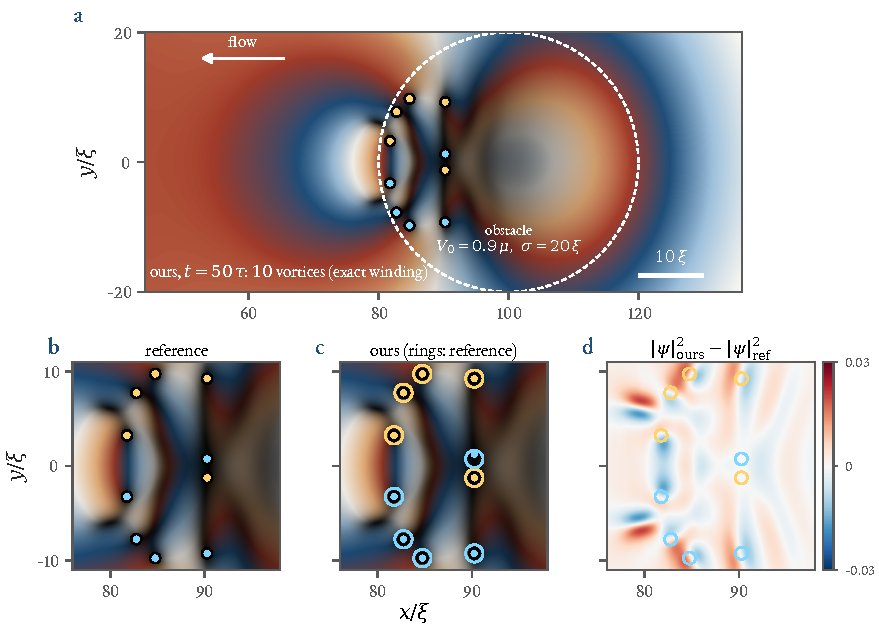
\includegraphics[width=\linewidth]{figures/ch09_wake.pdf}
\caption[The wake at $t=50\,\tau$]{The wake at $t=50\,\tau$. Hue is the phase of $\psi$, brightness its modulus (a hole in the fluid is black); the dots are plaquettes of non-zero winding (counter-clockwise gold, clockwise cyan; \cref{ch09:count}). \textbf{a}, our field; the dashed circle is the $1/\mathrm e^2$ radius of the obstacle and the fluid streams from right to left. \textbf{b}, \textbf{c}, the vortex region of the deposited field and of ours at eight times the grid resolution (spectral interpolation); the rings in \textbf{c} are the deposited vortices. \textbf{d}, $|\psi|^2_{\rm ours}-|\psi|^2_{\rm ref}$, at most $\cnineMaxDnFifty$ on the grid. Script \texttt{figures/ch09\_wake.py}.}\label{ch09:fig-wake}
\end{figure}

\Cref{ch09:fig-wake} is the picture to keep in mind. The broad lobes of colour are the phase of the potential flow around the obstacle. In panel \textbf{a} the ten dots are vortices, five pairs, each vortex the mirror image of an antivortex across the axis of the flow. The dark arcs through them are density troughs, lines on which the density is far below its bulk value. The deposited field and ours cannot be told apart at this magnification; panel \textbf{d} shows where they differ.

\section{The deposited run and the model}\label{ch09:model}

\paragraph{The archive.} The archive that accompanies the paper (Zenodo, version 1.0.0, 2026; code under the MIT licence, processed data to be reused with attribution under CC BY 4.0, as its README says \cite{KwonShin2026data}) holds the processed data behind the paper's summary figures (drag, lift and Strouhal number against a superfluid Reynolds number), the authors' GPU code (CuPy) with its configuration file, and one raw output case, for an obstacle of height $V_0=0.9\,\mu$ and width $\sigma=20\,\xi$ in a flow of $0.55$ times the speed of sound. For that case it gives the force on the obstacle every $0.1\,\tau$ and the output of the code's vortex detector every $5\,\tau$, both up to $t=100\,\tau$, and snapshots of the wave function every $10\,\tau$ from $t=0$ to $t=50\,\tau$. The README says what is not there: the full raw trajectories behind the paper's averages.

\paragraph{What we reproduce, and what we do not.} We reproduce the one raw case. We do not reproduce the paper's results, which rest on many parameter sets, each averaged over a window $\cninePaperTLo\le t\le\cninePaperTHi\,\tau$ \cite{KwonShin2026prr}, and on a post-processing (time-averaged irrotational flow, Mach-1 contour, effective diameter, Fourier analysis of the force) that we did not implement. Its central claims, a transition from periodic emission of vortex dipoles to the shedding of alternating same-sign vortex clusters at a superfluid Reynolds number $\mathrm{Re}_s\approx\cninePaperRes$ and the collapse of the Strouhal number and of the drag coefficient onto universal curves against $\mathrm{Re}_s$, are quoted as the authors' and not as ours. For the obstacle of the deposited case the paper reports a critical velocity $v_c\approx\cninePaperVc$ for dipole emission and a transition to cluster shedding at $v_{\rm th}\approx\cninePaperVth$ (in units of the speed of sound; every number of the paper quoted in this chapter is that of its arXiv version 1); the deposited run, at $0.55$, lies well above both.

\paragraph{The model.} In the units in which $\hbar=m=\mu=g=1$, the unit of length is the healing length $\xi=\hbar/\sqrt{m\mu}$, the unit of time is $\tau=\hbar/\mu$, the speed of sound of the uniform fluid is $c=\sqrt{\mu/m}=1$, the bulk density is $1$, and forces are measured in $\mu/\xi$. The deposited code integrates
\begin{equation}\label{ch09:eq-model}
\partial_t\psi \;=\; v(t)\,\partial_x\psi\;-\;\bigl(\mathrm i+\Gamma(x,y)\bigr)\Bigl[-\tfrac12\nabla^2+|\psi|^2-1\Bigr]\psi\;-\;\mathrm i\,V(x,y)\,\psi ,
\end{equation}
\begin{equation}\label{ch09:eq-pot}
V=V_0\exp\!\Bigl[-\frac{2\,\bigl((x-x_{\rm obs})^2+y^2\bigr)}{\sigma^2}\Bigr],\qquad v(t)=v_{\rm f}\,\min\!\bigl(t/t_{\rm acc},\,1\bigr),
\end{equation}
with $V_0=0.9$, $\sigma=20$, $x_{\rm obs}=100$, $v_{\rm f}=0.55$ and $t_{\rm acc}=0.1$, on a periodic grid of $1000\times500$ points of spacing $0.5\,\xi$ that covers $[-250,250)\times[-125,125)\,\xi$, with the time step $\Delta t=0.01\,\tau$. Read it term by term. Without $v$, $\Gamma$ and $V$ it is the Gross--Pitaevskii equation of \cref{ch03} with the chemical potential subtracted. The term $v\,\partial_x\psi$ moves to the frame of the obstacle: far away the fluid is at rest in the laboratory, the obstacle moves along $+x$ at speed $v$, and in the frame of the obstacle the fluid streams towards $-x$. The phase $\theta$ of $\psi$ is the laboratory phase, so the velocity relative to the obstacle is $\mathbf u=\nabla\theta-v\,\mathbf e_x$. The box is $500\,\xi\times250\,\xi$ and the obstacle sits at $x=100\,\xi$, so that the wake has $350\,\xi$ to run in. The damping function $\Gamma$ is $\cnineGammaCentre$ at the centre of the obstacle and at most $\cnineGammaDisc$ within its $1/\mathrm e^2$ radius, and rises to $\Gamma_0=0.1$ across layers that begin $50\,\xi$ and $40\,\xi$ from the edges of the box; in the layers the factor $(\mathrm i+\Gamma)$ turns the Hamiltonian evolution into a damped one, which absorbs the sound that the obstacle radiates before it can return through the periodic boundaries. The obstacle enters only through $-\mathrm iV\psi$: the deposited code treats $V$ as unitary and does not multiply it by the damping. The obstacle is \emph{penetrable} because $V_0<\mu$: at rest, the Thomas--Fermi density at its centre is $1-V_0=\cnineCoreDensity$ of the bulk, not zero.

Equation \eqref{ch09:eq-model} is what we recovered from the deposited code. The paper's own equation (1) agrees with it in its Hamiltonian part, and describes the damping layer (the ``fringe region'') with other numbers than the code does ($w_x=\cninePaperWx\,\xi$, $w_y=\cninePaperWy\,\xi$ and a transition scale $d=\cninePaperD\,\xi$, against layers of $50\,\xi$ and $40\,\xi$ and a scale of $15\,\xi$ in the code). We follow the code, because it is what produced the deposited run, and we have not tried to find out whether the two descriptions are equivalent in some convention.

\paragraph{Two schemes.} The deposited code advances \eqref{ch09:eq-model} by a splitting of Strang type: half a step of the linear part (kinetic term, moving-frame term, damping of the kinetic term) by a fourth-order Runge--Kutta method, a full step of the local part (nonlinearity, potential, constant offset) integrated exactly, and a second half step of the linear part, in single precision (\texttt{complex64}) on a GPU, with $\Delta t=0.01\,\tau$. Our scheme integrates the whole right-hand side of \eqref{ch09:eq-model} with one explicit fourth-order Runge--Kutta step, evaluates the derivatives spectrally, works in double precision, and uses the same $\Delta t$; we start it from the deposited field at $t=0$. The two computations therefore share the model and the initial data, and nothing else: not the scheme, not the precision, not the order of operations, not the machine. If they agree, the agreement is about the model and the data, not about a shared discretisation.

\paragraph{The force.} The force on the obstacle is the deposited code's
\begin{equation}\label{ch09:eq-force}
F_x=\iint \partial_xV\,|\psi|^2\,\mathrm dx\,\mathrm dy ,
\end{equation}
taken over the interior of the damping layers ($|x|<200\,\xi$, $|y|<85\,\xi$), with central differences for $\partial_xV$ and the trapezoidal rule, exactly as the code does. It is negative, the fluid pushing the obstacle along the flow, and we plot the drag $D=-F_x$. (The paper writes the force on the fluid, which is the opposite.) The lift $F_y$ is the same integral with $\partial_yV$.

\section{Why a subsonic flow can dissipate}\label{ch09:landau}

\paragraph{Landau's criterion.} An object of mass $M$ moves at speed $v$ through a fluid at rest. It can slow down only by creating an excitation of momentum $\hbar k$ and energy $\varepsilon(k)$, and conservation of energy and momentum then allows this only if
\begin{equation}\label{ch09:eq-landau}
v\;\ge\;\frac{\varepsilon(k)}{\hbar k}\quad\text{for some }k,\qquad\text{i.e.}\qquad v\;\ge\;v_{\rm L}:=\min_k\frac{\varepsilon(k)}{\hbar k}
\end{equation}
(for $M$ large against the excitation). Below $v_{\rm L}$ the object cannot dissipate energy into the fluid \cite{Landau1941}. The criterion needs one input, the spectrum $\varepsilon(k)$ of the elementary excitations of the fluid at rest.

\begin{godfrinbox}{The spectrum behind the criterion}
For superfluid $^4$He that spectrum is the dispersion curve of the Landau elementary excitations (phonon, maxon, roton) that Godfrin and his collaborators measured by inelastic neutron scattering at the ILL spectrometer IN5, and whose thermodynamic consequences they drew \cite{Godfrin2021}. In the review he wrote with Krotscheck, Landau's argument takes one paragraph \cite{GodfrinKrotscheck2022}: the creation of excitations by an object displaced in the fluid is impossible unless its velocity exceeds a critical value, and ``The linearity of the dispersion relation at low wave vectors is essential for this to happen''; in a Bose gas, whose dispersion is parabolic, the critical velocity is zero. These are statements about a curve that was \emph{measured}. The two lemmas below prove the inequalities behind them; they know nothing about helium, and nothing about the curve.
\end{godfrinbox}

\begin{leanbox}{HeliumKinematics}
\begin{lstlisting}[style=lean]
theorem landau_velocity_parabolic_zero {a : ℝ} (ha : 0 < a)
    {v : ℝ} (hv : 0 < v) :
    ∃ k : ℝ, 0 < k ∧ a * k ^ 2 / k < v := by
  refine ⟨v / (2 * a), by positivity, ?_⟩
  -- (proof abridged: three more lines)

theorem landau_velocity_ge_of_above_sound_line {ε : ℝ → ℝ}
    {c k : ℝ} (hk : 0 < k) (h : c * k ≤ ε k) : c ≤ ε k / k := by
  rw [le_div_iff₀ hk]; exact h
\end{lstlisting}
\end{leanbox}

In words: for a parabolic spectrum $\varepsilon=ak^2$ the ratio $\varepsilon/k=ak$ falls below any $v>0$ (take $k=v/2a$), so $v_{\rm L}=0$; a spectrum on or above the sound line $ck$ has $\varepsilon/k\ge c$ at every $k$. They are \Lthm{HeliumKinematics}{landau_velocity_parabolic_zero} and \Lthm{HeliumKinematics}{landau_velocity_ge_of_above_sound_line}, formalised from the review's paragraph, and they are theorems about real numbers, not about the experiment.

\paragraph{The uniform Gross--Pitaevskii fluid.} For the model \eqref{ch09:eq-model} the excitations of the uniform fluid are Bogoliubov's \cite{Bogoliubov1947}: in our units $\varepsilon(k)^2=\tfrac{k^2}2\bigl(\tfrac{k^2}2+2\bigr)$, that is $\varepsilon(k)=k\sqrt{1+k^2/4}$ (see \cref{ch05}). The following two statements are new Lean, written for this chapter (file \texttt{book/lean/Ch09\_FlowPast.lean}, namespace \texttt{QuantumFluids.FlowPast}; they are not part of the library). Compiled with Lean 4.34.0-rc2 and the matching Mathlib; no \texttt{sorry}; axioms \texttt{propext}, \texttt{Classical.choice}, \texttt{Quot.sound}.

\begin{leanbox}[title={Lean 4 \enspace FlowPast (new for this book)}]{Ch09\_FlowPast (new)}
\begin{lstlisting}[style=lean]
noncomputable def bogEps (k : ℝ) : ℝ := k * Real.sqrt (1 + k ^ 2 / 4)

theorem bogEps_ge_sound {k : ℝ} (hk : 0 ≤ k) : 1 * k ≤ bogEps k

theorem landau_uniform_gp :
    (∀ k : ℝ, 0 < k → 1 ≤ bogEps k / k) ∧
    (∀ δ : ℝ, 0 < δ → ∃ k : ℝ, 0 < k ∧ bogEps k / k < 1 + δ)
\end{lstlisting}
\end{leanbox}

The Landau velocity of the uniform Gross--Pitaevskii fluid is exactly the speed of sound (\Lthm{FlowPast}{landau_uniform_gp}): the ratio $\varepsilon/k$ never falls below $1$, and it comes within any $\delta$ of $1$, at $k=\sqrt{2\delta}$, where it equals $\sqrt{1+\delta/2}$ (proof abridged: the first clause is $\sqrt{1+k^2/4}\ge1$, the second is that identity and $\sqrt{1+\delta/2}<1+\delta$). The infimum is approached for $k\to0$ and never attained. Our obstacle moves at $0.55<1$. For the uniform fluid, \eqref{ch09:eq-landau} forbids every excitation, and the run nevertheless dissipates. (\Cref{ch05} proves the same statement for general $c$ and $m$: \Lthm{BogoliubovDispersion}{landau_velocity_eq}.)

\paragraph{The hypothesis that fails.} Landau's argument is about excitations of a fluid that is uniform, and an obstacle that disturbs it little. An obstacle of height $0.9\,\mu$ is not a small disturbance. At rest, the density in its core is a tenth of the bulk, and the local speed of sound there is $\sqrt{\cnineCoreDensity}=\cnineCoreSound$; a fluid forced through or around it must speed up. The criterion has to be applied locally, the local density fixing the local speed of sound. That is how Kwon and Shin read it: nucleation sets in when the flow becomes locally supersonic, $v(\mathbf r)>c_s(\mathbf r)=\sqrt{g\rho(\mathbf r)/m}$ (their equation (5), which they call the local Landau criterion), and they build their effective diameter, and with it their Reynolds number, on the Mach-1 contour of the time-averaged irrotational flow \cite{KwonShin2026prr}. The idea is older. Frisch, Pomeau and Rica found in the Gross--Pitaevskii model that vortex pairs are emitted behind an obstacle \cite{FrischPomeauRica1992}, and Josserand, Pomeau and Rica related the nucleation around a disk to the flow becoming locally supersonic at its edge \cite{JosserandPomeauRica1999}.

The following statements make the local criterion exact. They are again new Lean, in the same file.

\begin{leanbox}[title={Lean 4 \enspace FlowPast (new for this book)}]{Ch09\_FlowPast (new)}
\begin{lstlisting}[style=lean]
theorem supersonic_iff {n j : ℝ} (hn : 0 < n) (hj : 0 < j) :
    Real.sqrt n < j / n ↔ n ^ 3 < j ^ 2

theorem sonic_speed_threshold {n u V B : ℝ} (hB : n + u ^ 2 / 2 + V = B) :
    n < u ^ 2 ↔ 2 / 3 * (B - V) < u ^ 2

theorem bernoulli_min {s n : ℝ} (hs : 0 < s) (hn : 0 < n) :
    3 / 2 * s ≤ s ^ 3 / (2 * n ^ 2) + n

theorem barrier_height_bound {s n V : ℝ} (hs : 0 < s) (hn : 0 < n)
    (hB : s ^ 3 / (2 * n ^ 2) + n + V = 1 + s ^ 3 / 2) :
    V ≤ (1 - s) ^ 2 * (s + 2) / 2
\end{lstlisting}
\end{leanbox}

\emph{The first} (\Lthm{FlowPast}{supersonic_iff}) says that a flow of density $n$ and local flux $j=nu$ has $u>\sqrt n$, the local speed of sound, exactly when $n^3<j^2$, that is when the density is below the \emph{sonic density} $j^{2/3}$. It is algebra, and it is the form in which the data will be read below. \emph{The second} (\Lthm{FlowPast}{sonic_speed_threshold}) adds Bernoulli's relation $n+\tfrac12u^2+V=B$, the stationary hydrodynamic relation without quantum pressure, with $B=1+\tfrac12v^2$ for a fluid of density $1$ at speed $v$ far from the obstacle: the flow is locally supersonic exactly when $u^2>\tfrac23(B-V)$, a threshold on the speed that depends on the potential only. For $V=0$ it is the critical speed $u^2=\tfrac23+\tfrac13v^2$ that Josserand, Pomeau and Rica obtained for the flow past a disk; here it is $\cnineUcFar$ far from the obstacle, and $\cnineUcCentre$ at the centre of the obstacle, where $V=V_0=0.9$.

\emph{The last two} are a one-dimensional picture of the same mechanism. Take a steady flow in a channel, of flux $j$ conserved along the channel, and write $j^2=s^3$, so that $s$ is the sonic density. Bernoulli's function $j^2/(2n^2)+n$ is bounded below by $\tfrac32s$ (\Lthm{FlowPast}{bernoulli_min}), with equality only at the sonic point $n=s$ (\Lthm{FlowPast}{bernoulli_eq_iff}, in the file). The proof is a factorisation: $\frac{s^3}{2n^2}+n-\frac32s=\frac{(n-s)^2(2n+s)}{2n^2}\ge0$, the identity $2n^3-3sn^2+s^3=(n-s)^2(2n+s)$ being checked by \texttt{ring} (proof abridged). Consequently, if the fluid upstream has density $1$ and speed $j$, a steady state can exist at a point of the channel where the potential is $V$ only if $V\le V_c(s):=(1-s)^2(s+2)/2$ (\Lthm{FlowPast}{barrier_height_bound}): there is no steady flow over a barrier higher than that, the flow is \emph{choked}. For $j=0.55$ the sonic density is $s=\cnineSonicS$ and the ceiling is $V_c=\cnineVc$; the obstacle's $V_0=0.9$ is $\cnineVzeroOverVc$ times higher. As $j\to1$ (so $s\to1$) the ceiling $V_c$ tends to $0$: at the speed of sound any barrier chokes the flow, which is Landau's criterion again, seen from the other side.

\paragraph{What the one-dimensional theorem is not.} The ceiling $V_c$ reaches $V_0=0.9$ at $j=\cnineJatVc$, a factor of ten below the critical velocity $v_c\approx\cninePaperVc$ that Kwon and Shin find for the two-dimensional flow by testing for stationary solutions. The theorem does not predict that threshold, and LL-15, the programme's rule that an analogy is not a result, says why: it needs a flux conserved along the channel, and the flow has none. On the axis of the deposited run at $t=20\,\tau$ the flux at the centre of the obstacle is $j=\cnineAxisJcentre$, $\cnineAxisJratio\,\%$ of the upstream $0.55$: the stream lines have opened up. What survives is the structure of the picture, the sonic point as the minimum of Bernoulli's function and the supersonic region as the part of the flow beyond it. Kwon and Shin's own estimate of the supersonic region (their appendix A) uses Bernoulli and continuity in two dimensions to first order in $v/c$; they report that it overestimates the threshold and attribute the difference to the neglected quantum pressure, which they say is crucial in triggering shedding. The data below agree.

\paragraph{Reading the data.} \Cref{ch09:fig-mach} shows the field at $t=20\,\tau$, four time units before the first pair. The supersonic region is a single blob inside the obstacle, on its downstream half: on the axis it runs from $x=\cnineAxisSupLo$ to $\cnineAxisSupHi$ (the obstacle is centred at $100$), and it extends at most $\cnineSupYhalfOursTwenty\,\xi$ to either side. Its area is $\cnineSupAreaOursTwentyP\,\xi^2$ in our field and $\cnineSupAreaRefTwentyP\,\xi^2$ in the deposited one; the Mach number reaches $\cnineSupMOursTwenty$ and $\cnineSupMRefTwenty$ at $x=\cnineSupXMmax$, where the density is $\cnineAxisNmin$ and the flow runs at $\cnineAxisSpeedMax\,c$ relative to the obstacle; the two $M=1$ contours cannot be told apart. The blob existed earlier: its area is $\cnineSupAreaOursTen$ and $\cnineSupAreaRefTen\,\xi^2$ at $t=10$ and $\cnineSupAreaOursFive\,\xi^2$ at $t=5$ (maximal $M$: $\cnineSupMOursTen$, $\cnineSupMRefTen$ and $\cnineSupMOursFive$). The local criterion is thus satisfied for at least nineteen time units before the first pair appears: necessary, but nowhere near sufficient on a short time scale. The region has to deepen, the rarefaction behind it has to sharpen, and then a hole opens at its downstream end (the star in \cref{ch09:fig-mach}\textbf{a}).

\begin{figure}[t]\centering
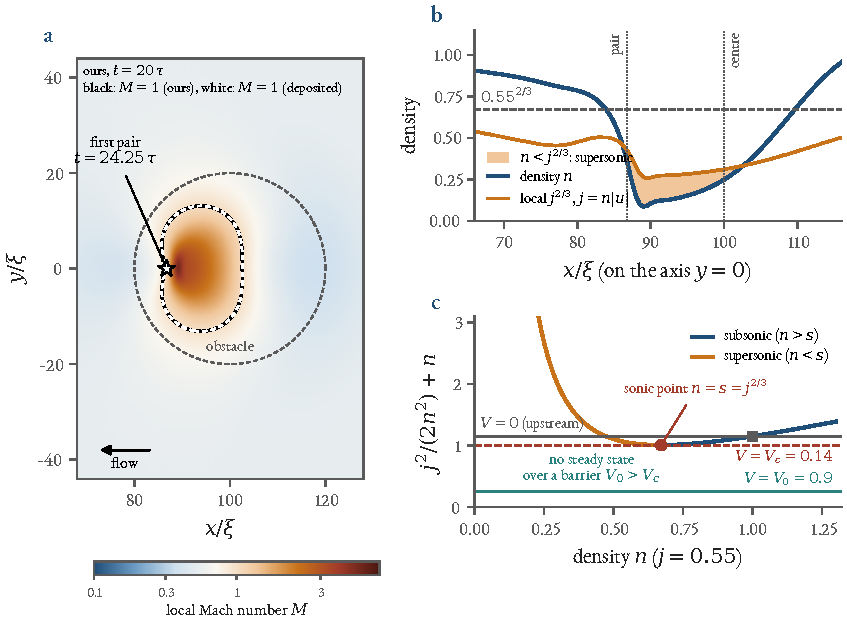
\includegraphics[width=\linewidth]{figures/ch09_mach.pdf}
\caption[The flow is locally supersonic long before the first vortex]{The flow is locally supersonic long before the first vortex. \textbf{a}, the local Mach number $M=|\nabla\theta-v\mathbf e_x|/\sqrt n$ of our field at $t=20\,\tau$; black, $M=1$ for our field; white dashes, $M=1$ for the deposited field; the star marks the first vortex pair, $t\approx24.25\,\tau$. \textbf{b}, the density and the local sonic density $j^{2/3}$, $j=n|\mathbf u|$, on the axis: $M>1$ exactly where $n<j^{2/3}$ (\lean{supersonic\_iff}). \textbf{c}, Bernoulli's function $j^2/(2n^2)+n$ of the channel at $j=0.55$ and the levels $1+j^2/2-V$ it must equal (\lean{bernoulli\_min}, \lean{barrier\_height\_bound}). Script \texttt{figures/ch09\_mach.py}.}\label{ch09:fig-mach}
\end{figure}

The threshold of \lean{sonic\_speed\_threshold} can be compared with this region without using the density. At $t=20$ the set where $|\mathbf u|^2>\tfrac23(B-V)$ has an area of $\cnineThrAreaOursTwenty\,\xi^2$ against the measured $\cnineMachAreaNearOursTwenty\,\xi^2$ and contains $\cnineThrInOursTwenty\,\%$ of it (at $t=5$, $10$, $15$: $\cnineThrInOursFive$, $\cnineThrInOursTen$, $\cnineThrInOursFifteen\,\%$), with an excess of area of $\cnineThrExcessOursFive\,\%$ at $t=5$ and $\cnineThrExcessOursTwenty\,\%$ at $t=20$. It predicts where the flow is supersonic well and what the density is poorly: Bernoulli's relation implies a density of $\cnineNBernCentre$ at the centre of the obstacle, where the measured one is $\cnineNMeasCentre$, because it needs a stationary flow (\cref{ch09:birth}).

\section{The reproduction}\label{ch09:repro}

\begin{keybox}[What ``reproduce'' means here]
Three things hide in the word. (i) The same input gives the same output, to rounding: the initial field is reproduced this way. (ii) A different scheme gives the same observables within a tolerance: for $t\le10$ the force agrees to $\cnineForceRelTen$ of its largest value, against a registered tolerance of $10^{-5}$ that was not met. (iii) The same events happen at the same times: the first vortex pair, the vortex counts. The fourth thing, reproducing the paper, is none of these and is not claimed.
\end{keybox}

\paragraph{What was run.} The flow solver is the module \texttt{flow} of the crate \texttt{qf-pgpe} (rusty-SUNDIALS, release v11.6.0; the Python extension \texttt{qf\_pgpe} does not expose it). It is driven by the example program \texttt{kwon\_shin}, which reads the deposited initial field and force, integrates, and writes the force every $0.1\,\tau$ and $\psi$ every $5\,\tau$. The production run to $t=50\,\tau$ took $\cnineProdSteps$ steps and $\cnineProdWall\,$s on the shared eight-core machine (load not recorded). Two excerpts of the source follow: the right-hand side \eqref{ch09:eq-model} (\texttt{ws.lap} is $\nabla^2\psi$, \texttt{ws.dxp} is $\partial_x\psi$, both spectral) and the velocities of the four stages.

\begin{rustbox}{qf-pgpe::flow, the source}
\begin{lstlisting}[style=rust]
// FlowSolver::rhs, last loop (excerpt)
for i in 0..psi.len() {
    let p = psi[i];
    let h = ws.lap[i] * (-0.5) + p * (p.norm_sqr() - 1.0);
    out[i] = ws.dxp[i] * v
        - (Complex64::new(self.gamma[i], 1.0)) * h
        - Complex64::new(0.0, self.potential[i]) * p;
}
// FlowSolver::step (excerpt): the velocity of the four stages
let (v1, v2, v3, v4) = match ramp {
    Ramp::StepEnd => {
        let v = self.velocity(t + dt);
        (v, v, v, v)
    }
    Ramp::StageTimes => (
        self.velocity(t),
        self.velocity(t + 0.5 * dt),
        self.velocity(t + 0.5 * dt),
        self.velocity(t + dt),
    ),
};
\end{lstlisting}
\end{rustbox}

\begin{rustbox}{qf-pgpe::flow, a fresh run}
A fresh run of the first time unit, made for this chapter (command, output and two rows of the force file as written; the path is shortened):
\begin{lstlisting}[style=plainmono]
$ kwon_shin --ref-dir .../20068724/extracted --t-end 1.0 --dt 0.01 --ramp step-end
step 0/100 t = 0.00 (1 s)
step 100/100 t = 1.00 (1169 s)
force_x: max |ours - reference| = 5.396e-6, relative to max |F| = 8.10e-6; wall 1169 s (100 steps)

t,force_x,force_ref,diff
0.300,-0.178067868131,-0.178068995476,1.127e-6
1.000,-0.665855021696,-0.665849626064,-5.396e-6
\end{lstlisting}
The hundred steps cost $\cnineFreshCpu\,$s of CPU time ($\cnineFreshPerStep\,$s per step, one thread) and $\cnineFreshWall\,$s of wall-clock time: the machine is shared (load average $\cnineFreshLoadA$ at the start, $\cnineFreshLoadB$ at the end), so the wall-clock figure measures the queue and not the code. The force column equals the first rows of the $\cnineProdSteps$-step run at the printed precision.
\end{rustbox}

\paragraph{The velocity ramp, and a convention that Lean can measure.} The deposited driver loops \texttt{for i in range(steps + 1): tt = i * dt; if i > 0: evolver.time\_evolv(tt)}, and \texttt{time\_evolv(tt)} uses $v(tt)$ in all of its stages. The step that takes the field from $(i-1)\Delta t$ to $i\Delta t$ therefore runs at the velocity of its \emph{end}. During the ramp ($0.1\,\tau$, ten steps) the obstacle moves relative to the fluid by $\sum_{i=1}^{10}v(i\Delta t)\Delta t=\cnineSumV$ instead of $\int_0^{0.1}v\,\mathrm dt=\cnineIntV$, an overshoot of $\cnineOvershoot\,\xi$. In general:

\begin{leanbox}[title={Lean 4 \enspace FlowPast (new for this book)}]{Ch09\_FlowPast (new)}
\begin{lstlisting}[style=lean]
theorem ramp_overshoot (a h : ℝ) (n : ℕ) :
    ∑ i ∈ range n, a * (((i : ℝ) + 1) * h) * h - a * ((n : ℝ) * h) ^ 2 / 2
      = a * h ^ 2 * n / 2
\end{lstlisting}
\end{leanbox}

Holding the velocity $at$ of a linear ramp at the end of each of $n$ steps of size $h$ overshoots the integral $a(nh)^2/2$ by exactly $ah^2n/2$ (\Lthm{FlowPast}{ramp_overshoot}; proof: induction on $n$ with one \texttt{nlinarith} for the step; abridged); with $a=v_{\rm f}/t_{\rm acc}=5.5$, $h=0.01$ and $n=10$ this is the $\cnineOvershoot$ above. The solver measures the same thing. With the velocity read at the stage times the force differs from the deposited one by $\cnineRampOffset$ at $t=0.1\,\tau$ (between $\cnineStageMin$ and $\cnineStageMax$ up to $t=5$); with the reference's reading it differs by $\cnineForceTc$ for $t\le0.3$. Halving $\Delta t$ halves the overshoot, to $\cnineOvershootHalf\,\xi$, and the offset goes down to $\cnineRampOffsetHalf$; the offsets are the same multiple of the displacement that separates the two runs, $\cnineSensA$ and $\cnineSensB\;\mu/\xi^2$. The convention is a displacement of the obstacle relative to the fluid by the amount that the theorem computes. It also means that halving $\Delta t$ with the reference's convention is not a convergence test, since the convention depends on $\Delta t$. Our own temporal error, with the stage-time reading, is $\cnineOwnTemporal$ in the force over $t\le5$ ($\Delta t=0.01$ against $0.005$), negligible against every other number in this chapter.

The library module \texttt{HeliumKinematics} does the same kind of small job for the analysis of the neutron time-of-flight data of the 2021 paper: it proves that two printed energy formulas (its equations 12 and 13) are one formula once the flight distance and the incident energy are written through the incident velocity (\Lthm{HeliumKinematics}{tof_eq12_eq_eq13}) and that rescaling the energy calibration cannot change whether one measured energy exceeds twice another (\Lthm{HeliumKinematics}{plateau_excess_calibration_invariant}): what a convention can and cannot move, settled once. The resemblance is one of method; it says nothing about neutron scattering.

\paragraph{The initial field.} The deposited initial field is itself a finding. The code prepares it by imaginary-time propagation from the Thomas--Fermi field, stopping when the integral $\gamma$ of $|\psi_{\rm new}-\psi_{\rm old}|^2$ falls below $\epsilon\,\delta\tau$, with the deposited tolerance $\epsilon=\cnineEps$ and $\delta\tau=0.04$, that is below $\cnineStopThr$. We re-derived the field in a few lines of numpy from the code's operators. After \emph{one} step $\gamma=\cnineGammaOne<\cnineStopThr$: the loop stops at its first iteration. The stored $\psi(t=0)$ is therefore the Thomas--Fermi field after one imaginary-time step plus the seeded noise ($10^{-4}$ times integers in $[-5,5)$ for the real and the imaginary part, relative size $\cnineInitNoise$), not a relaxed stationary state of the obstacle problem. Our array, rounded to \texttt{complex64}, equals the stored one bit for bit in $90\,\%$ of its $\cnineInitN$ elements; the other $\cnineInitDiffN$ (those where the noise has a zero imaginary part) differ by floating-point residues below $2\times10^{-16}$. In double precision the distance is $\cnineInitDouble$, the rounding of \texttt{complex64}. This is a statement about the deposited data and not a criticism of the paper, which describes the initial state as relaxed to the ground state and measures its observables long after any relaxation of the initial field; but anyone who uses the deposited $\psi(0)$ as a ground state should know that the early force contains that relaxation.

\paragraph{Results.} \Cref{ch09:tab-repro} collects the comparisons, \cref{ch09:fig-force} shows the force. All numbers are computed by \texttt{figures/ch09\_numbers.py} from the deposited files and our snapshots.

\begin{table}[t]\centering\small
\begin{tabular}{@{}p{0.31\linewidth}p{0.63\linewidth}@{}}\toprule
quantity & ours against the deposited run\\\midrule
initial field & bit for bit after rounding to \texttt{complex64} in $90\,\%$ of the elements; $\cnineInitDouble$ in double precision\\
force $\max|\Delta F|$, $t\le0.3$; $<1$; $\le5$; $\le10$ & $\cnineForceTc$; $\cnineForceLtOne$; $\cnineForceFive$; $\cnineForceTen$ ($\cnineForceRelTenTwo$ of the largest force, $\cnineForceMaxTen$, of that window)\\
force, windows $10$--$20$, $20$--$30$, $30$--$40$, $40$--$50$ & $\cnineForceTwenty$; $\cnineForceThirty$; $\cnineForceForty$; $\cnineForceFifty$ ($\cnineForceOverallPct\,\%$ of the largest force, $\cnineForceMax$)\\
$\psi$ at $t=10,20,30,40,50$ (relative $L^2$) & $\cninePsiTen$, $\cninePsiTwenty$, $\cninePsiThirty$, $\cninePsiForty$, $\cninePsiFifty$; after removing a global phase $\cninePsiGaugeTen$, $\cninePsiGaugeTwenty$, $\cninePsiGaugeThirty$, $\cninePsiGaugeForty$, $\cninePsiGaugeFifty$\\
density $|\psi|^2$ (relative $L^2$) & $\cnineDensTen$, $\cnineDensTwenty$, $\cnineDensThirty$, $\cnineDensForty$, $\cnineDensFifty$\\
lift $F_y$ at the snapshot times & within $\cnineLiftRelMin$--$\cnineLiftRelMax\,\%$ of the deposited values ($|F_y|\le\cnineLiftMax$)\\
vortex census, $t=30,40,50$ & $\cnineMatchTotalIdent$ of $\cnineMatchTotal$ vortices on the same plaquette, one within one cell\\
count of the deposited detector & equal at $\cnineEqualCounts$ of $10$ times\\
supersonic region, $t=20$ & area $\cnineSupAreaOursTwentyP$ against $\cnineSupAreaRefTwentyP\,\xi^2$; $M_{\max}$ $\cnineSupMOursTwenty$ against $\cnineSupMRefTwenty$\\
own temporal error & $\cnineOwnTemporal$ in the force, $t\le5$\\\bottomrule
\end{tabular}
\caption{Our Rust run against the deposited run. Every row is recomputed here from the raw files. The rows on the initial field, the force, $\psi$, the density and the detector's counts repeat numbers of the programme's earlier record (\texttt{docs/designs/PGPE\_EXTERNAL\_REPRODUCTION.md}); the gauge-fixed distances, the lift, the census and the supersonic region are new.}\label{ch09:tab-repro}
\end{table}

\begin{figure}[t]\centering
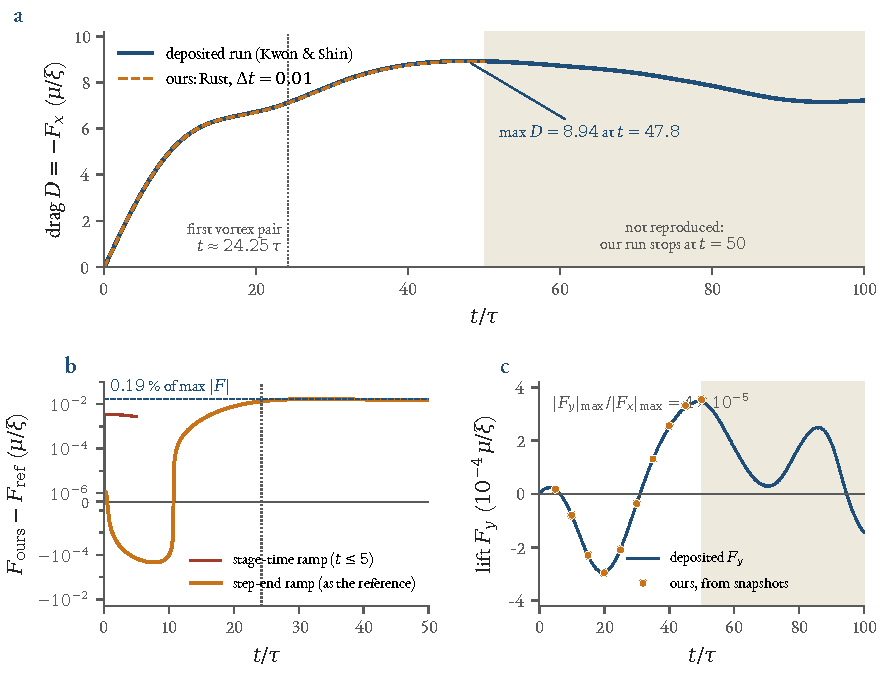
\includegraphics[width=\linewidth]{figures/ch09_force.pdf}
\caption[The force on the obstacle]{The force on the obstacle. \textbf{a}, the drag $D=-F_x$ of the deposited run to $t=100\,\tau$ (blue) and of our Rust run to $t=50\,\tau$ (orange dashes). \textbf{b}, the difference $F_{\rm ours}-F_{\rm ref}$ on a symmetric logarithmic axis, with the reference's step-end reading of the velocity (orange) and with the stage-time reading up to $t=5$ (red); the dotted line marks the first vortex pair. \textbf{c}, the lift $F_y$ of the deposited run and ours at the snapshot times. Script \texttt{figures/ch09\_force.py}.}\label{ch09:fig-force}
\end{figure}

Three things stand out. The agreement is at the level of $10^{-6}$ for the first time unit and $10^{-4}$ for the first ten, which is what two accurate integrators of the same equation should give, and it was reached with a scheme, a precision and a machine that have nothing in common with the reference's. Second, the tolerance that the programme had registered for this item of its plan, a relative force agreement of $10^{-5}$ for $t\le10$, is not met: it is $\cnineForceRelTen$ of the largest force of that window (it is $\cnineForceRelTc$ for $t\le0.3$). The criterion was set before the reference's velocity convention was known, and the plan keeps it as failed. No criterion had been registered for $t>10$; the second half of the table is reported as found. Third, from $t\approx\cnineZeroCross$ the force difference changes sign, grows, and levels off at about $\cninePlateauMean$, $\cnineForceOverallPct\,\%$ of the largest force, for $t\ge26$. \Cref{ch09:gaps} comes back to it, because the first reading of that growth that the programme gave is not supported by the data.

\section{Counting vortices}\label{ch09:count}

\paragraph{What a count is.} A vortex is a point where the wave function vanishes and its phase winds by $2\pi$; a grid sees only $\psi$ at its points. The standard way out, used by many vortex-finding codes, is to add up the \emph{principal differences} of the phase around each plaquette (an elementary square of four grid points) and to divide by $2\pi$. The proof assistant has something exact to say about that procedure: it rests on a statement that is true for a reason, and it fails for a reason.

\begin{leanbox}{VortexWinding}
\begin{lstlisting}[style=lean]
noncomputable def pdiff (a b : ℝ) : ℝ := toIocMod two_pi_pos (-π) (b - a)

theorem loop_sum_eq_mul (θ : ℕ → ℝ) (n : ℕ) (hclosed : θ n = θ 0) :
    ∃ m : ℤ, ∑ i ∈ Finset.range n, pdiff (θ i) (θ (i + 1))
      = (m : ℝ) * (2 * π) := by
  -- (proof abridged: pdiff = (b - a) - integer * 2π, then the sum telescopes)

theorem pdiff_add_rev_eq_two_pi_iff (a b : ℝ) :
    pdiff a b + pdiff b a = 2 * π ↔ (pdiff a b = π ∧ pdiff b a = π)
\end{lstlisting}
\end{leanbox}

The first theorem, \Lthm{VortexWinding}{loop_sum_eq_mul}, says that for \emph{any} closed list of phases $\theta_0,\dots,\theta_n=\theta_0$ the sum of the principal differences along the loop is an integer multiple of $2\pi$ (here \texttt{pdiff a b} is the representative of $b-a$ in $(-\pi,\pi]$): that a computed winding number is an integer is a theorem and not a numerical accident. The second says exactly when an edge fails to cancel. Walked in both directions an edge gives $0$, unless both principal differences equal $\pi$, which add up to $2\pi$; at that single value the cancellation between the two plaquettes that share the edge breaks, and a spurious winding can appear. With no edge at $\pi$ the oriented sum over a closed surface is zero (\Lthm{VortexWinding}{cut_free_of_ne_pi}, \Lthm{VortexWinding}{balanced_sum_eq_zero}), which for the plaquettes of a periodic grid means that the integer charges add up to zero. What the module does \emph{not} prove, in its own words, is that a field is resolved well enough for the detected winding to be the topological charge of the continuum field: that is a statement about sampling, and it is where data come in. The library's \lean{pdiff} and the Python function that we use are the same function:

\par\noindent\begin{minipage}{\linewidth}
\begin{lstlisting}[style=py]
def pdiff(a, b):
    d = (b - a + np.pi) % (2 * np.pi) - np.pi
    return np.where(d == -np.pi, np.pi, d)

def edge_steps(psi):
    th = np.angle(psi)
    return pdiff(th, np.roll(th, -1, 1)), pdiff(th, np.roll(th, -1, 0))

def plaquette_charge(psi):
    sx, sy = edge_steps(psi)
    s = sx + np.roll(sy, -1, 1) - np.roll(sx, -1, 0) - sy
    q = s / (2 * np.pi)
    return q, np.rint(q).astype(int)
\end{lstlisting}
\end{minipage}\par
\noindent (from \texttt{figures/ch09\_common.py}, docstrings omitted; the loop of \texttt{s} runs counter-clockwise around the plaquette whose lower-left corner is the grid point.) On the $\cnineWindN$ snapshots that we have, the six deposited fields and our ten, the unrounded charge \texttt{q} differs from an integer by at most $\cnineWindDev$, and the charges of every snapshot add up to zero. The largest principal step on any edge of any of the sixteen snapshots is $\cnineEdgeMax\,\pi$: the margin to the branch cut is $\cnineEdgeMargin\,\%$ of $\pi$, never zero.

\paragraph{Two counts.} The deposited run logs a vortex count every $5\,\tau$. It is the output of the authors' detector, the function that the same driver also hands to the routine that removes vortices near the boundary of the box. Its rule, from the code: take the local minima of the density along the first array axis ($y$) that are below $0.2$ and lie outside a disc of $5\,\xi$ around the obstacle; drop every minimum within $3\,\xi$ of an earlier one; keep a survivor if the phase circulation on the square loop of half-width $2\,\xi$ around it exceeds $0.9\pi$ in modulus, steps of $0.3\pi$ or more being \emph{dropped} from the sum. We ported this rule line by line (\texttt{exploration/external/ks\_vortex\_count.py}); on the deposited fields at $t=10,\dots,50$ it returns the deposited counts $0,0,3,4,7$. Alongside it we use the \emph{exact census}: every plaquette of non-zero winding, with no further rule. The two are compared in \cref{ch09:tab-census} and \cref{ch09:fig-census}.

\begin{table}[t]\centering\footnotesize
\setlength{\tabcolsep}{4pt}
\begin{tabular}{@{}lcccccccccc@{}}\toprule
$t/\tau$ & \cnineCensusHeader\\\midrule
\cnineCensusRows
\bottomrule\end{tabular}
\caption{Vortex counts. The first row is the deposited file, the second the same detector run on our snapshots, the last two the exact census of non-zero plaquettes (no deposited field exists at $t=5,15,\dots$).}\label{ch09:tab-census}
\end{table}

Three statements follow. \emph{First}, the detector's counts are equal at $\cnineEqualCounts$ of the ten times, with the single difference at $t=45$: $7$ in our run, $6$ in the deposited file. \emph{Second}, the census is identical at every time where a deposited field exists to compare with: $2$, $14$ and $10$ charged plaquettes at $t=30$, $40$, $50$ in both runs, and $\cnineMatchTotalIdent$ of the $\cnineMatchTotal$ on exactly the same plaquette, the last one within one cell ($0.5\,\xi$). This is a much stronger statement than the equal counts: not a number but the positions and signs of the vortices are reproduced. \emph{Third}, the detector is not a census. At $t=40$ it counts $4$ of the $14$ vortices that are present; at $t=30$ it counts $3$ where there are $2$, because two of its accepted loops enclose the same plaquette, so one vortex is counted twice (\cref{ch09:fig-census}\textbf{b}, \textbf{c}).

\begin{figure}[t]\centering
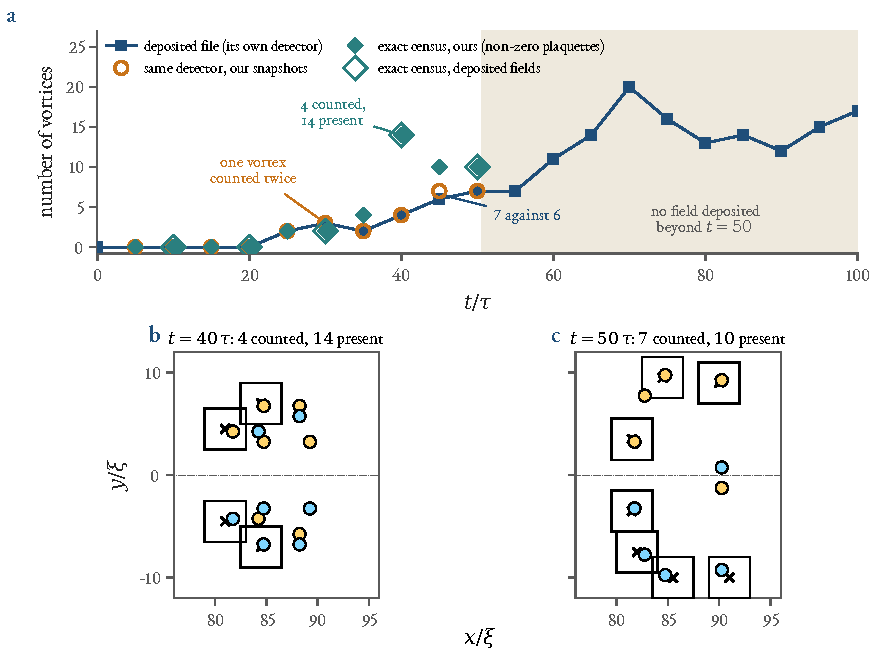
\includegraphics[width=\linewidth]{figures/ch09_census.pdf}
\caption[How many vortices?]{How many vortices? \textbf{a}, counts against time: the deposited file (blue squares, to $t=100\,\tau$), the same detector on our snapshots (open orange circles), and the exact census of non-zero plaquettes (teal diamonds: ours, filled; deposited fields, open). \textbf{b}, \textbf{c}, the deposited field at $t=40$ and $50\,\tau$: the plaquettes of non-zero winding (gold counter-clockwise, cyan clockwise) and, as black squares and crosses, the loops and centres of the detector's accepted vortices. Script \texttt{figures/ch09\_census.py}.}\label{ch09:fig-census}
\end{figure}

\paragraph{A fragile decision.} The detector's loop integral is not quantised, because it drops the large steps, and its decision is fragile. For the same vortex, the integral in the deposited field and in ours differs by up to $\cnineLoopDiffMax\,\pi$ (by $\cnineLoopDiffThirty\,\pi$ at $t=30$), against a threshold of $0.9\pi$, although the two fields agree to better than $\cninePsiFifty$ in relative $L^2$. At $t=45$, the one time at which the counts differ, no deposited field exists, so the vortex that the deposited detector missed cannot be identified. In our field the seven accepted vortices have loop integrals of $1.26\pi$ or more, except one, at $(x,y)=(\cnineMarginalX,-\cnineMarginalY)$, with $\cnineMarginalInt\,\pi$, which is $\cnineMarginalAbove\,\%$ above the threshold. It is the only candidate for which a perturbation of the size seen between the two runs at other times could flip the decision. That is a plausible explanation of the unit difference. It is not a demonstration.

\paragraph{Mirror symmetry.} The exact census is a set of mirror pairs: for each plaquette of charge $q$ at $(x,y)$ there is one of charge $-q$ at $(x,-y)$, in every snapshot of ours and in the deposited fields at $t=30$ and $40$; at $t=50$ the two plaquettes of the deposited field nearest to the axis have their partners one cell away. The relative $L^2$ distance of $\psi$ from its mirror image $\psi(x,-y)$ is $\cnineAsymZero$ at $t=0$ (the seeded noise), $\cnineAsymRefTen$ and $\cnineAsymOursTen$ at $t=10$ in the deposited field and in ours, and $\cnineAsymRefFifty$ and $\cnineAsymOursFifty$ at $t=50$: it decays instead of growing. Up to $t=50$ the flow is mirror-symmetric, and so, as far as the lift shows, is the deposited run up to $t=100$ (\cref{ch09:fig-force}\textbf{c}: the lift never exceeds $\cnineLiftRatio$ of the drag).

\section{The birth of a pair}\label{ch09:birth}

\paragraph{Zooming in time.} The snapshots are five time units apart; the first pair appears between two of them. To see it we continued our field from $t=20$ to $t=25$ with the same scheme in numpy (\texttt{figures/ch09\_birth\_run.py}), storing a $60\,\xi\times50\,\xi$ sub-box every $0.1\,\tau$. The continuation reproduces our Rust snapshot at $t=25$ to a relative $L^2$ distance of $\cnineContRel$: two implementations of one scheme, as they should be. \Cref{ch09:fig-birth} shows what happens.

\begin{figure}[t]\centering
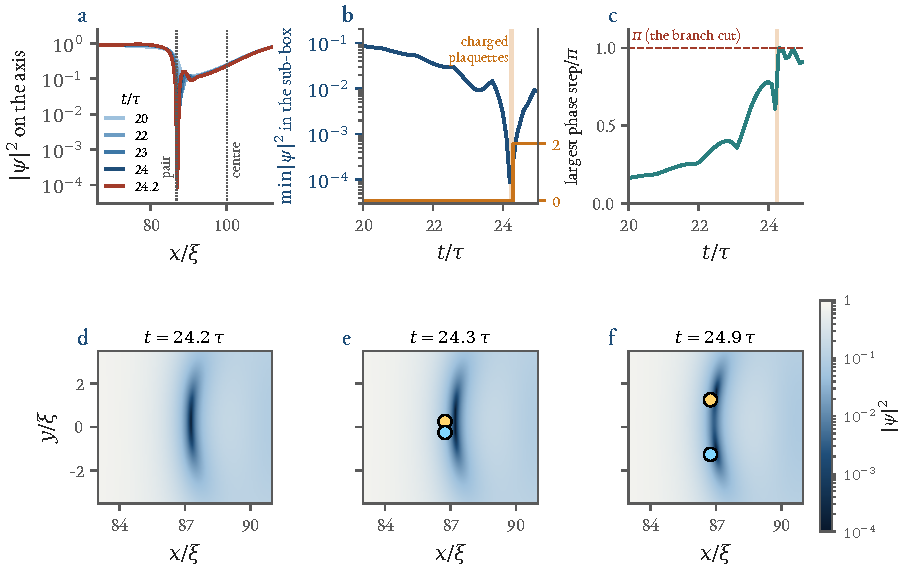
\includegraphics[width=\linewidth]{figures/ch09_birth.pdf}
\caption[The first vortex pair]{The first vortex pair, from the $0.1\,\tau$ continuation of our field. \textbf{a}, the density on the axis $y=0$ at five times; the dotted lines mark the birth site and the centre of the obstacle. \textbf{b}, the smallest density of the sub-box (blue, logarithmic) and the number of plaquettes of non-zero winding (orange); the shaded band is the interval in which the pair is born. \textbf{c}, the largest principal phase step on any edge of the sub-box, in units of $\pi$. \textbf{d}--\textbf{f}, the density (logarithmic colour scale, cubic interpolation) just before the birth, just after it and $0.6\,\tau$ later, with the charged plaquettes (gold counter-clockwise, cyan clockwise). Script \texttt{figures/ch09\_birth.py}.}\label{ch09:fig-birth}
\end{figure}

\paragraph{What happens.} On the axis the density minimum of the sub-box falls from $\cnineNminTwenty$ at $t=20$ to $\cnineNminTwentyThree$ at $t=23.3$, where it hesitates, and then, within a time unit, to $\cnineBirthNmin$ at $t=\cnineBirthBefore$. At $t=\cnineBirthAfter$ two plaquettes carry the charges $\mp1$, at $(x,y)=(\cnineBirthX,\mp\cnineBirthY)$: a vortex and an antivortex, $\cnineBirthSep\,\xi$ apart, on the axis, $\cnineBirthDist\,\xi$ downstream of the centre of the obstacle. Since the flow is mirror-symmetric a single pair has to be born on the axis, and it is. By $t=24.9$ the two are $\cnineBirthSepLate\,\xi$ apart. The pair appears at the downstream end of the supersonic region, which at $t=\cnineBirthAfter$ runs on the axis from $x=\cnineBirthSupLo$ to $\cnineBirthSupHi$: within a healing length of its edge.

\paragraph{Lean's edge case in the data.} The largest principal phase step on any edge of the sub-box is $\cnineEdgeTwentyFour\,\pi$ at $t=24.0$, $\cnineEdgeTwentyFourTwo\,\pi$ at $t=\cnineBirthBefore$ and $\cnineBirthEdge\,\pi$ at $t=\cnineBirthAfter$, the first time the pair exists (\cref{ch09:fig-birth}\textbf{c}). Two vortices of opposite sign one grid cell apart are the configuration in which the phase differs by almost $\pi$ across the edge that joins them. The branch cut that \Lthm{VortexWinding}{pdiff_add_rev_eq_two_pi_iff} isolates is therefore not a remote possibility: when the pair is born the largest step is within $0.2\,\%$ of $\pi$. No edge is exactly at $\pi$, so the census is an exact integer count of the sampled field. What that count means \emph{at birth} is not decided by the theorem. A pair half a healing length apart, on a grid whose spacing is half a healing length, is at the limit of what the sampled field resolves; resolution, not the theorem, decides whether the two plaquettes are two vortices of the continuum field.

\paragraph{Hydrodynamics on the data.} The reading of the run in terms of Bernoulli's relation and the supersonic region (\cref{ch09:landau}) rests on the Madelung form of \eqref{ch09:eq-model}. Write $\psi=\sqrt n\,\mathrm e^{\mathrm i\theta}$, $\mathbf u=\nabla\theta-v\,\mathbf e_x$ and $Q=-\nabla^2\!\sqrt n/(2\sqrt n)$, the quantum pressure. Where $\Gamma=0$, the phase obeys
\begin{equation}\label{ch09:eq-madelung}
-\partial_t\theta\;=\;R\;:=\;\tfrac12|\mathbf u|^2+n+V+Q-1-\tfrac12v^2 .
\end{equation}
For a stationary flow $R=0$: that is Bernoulli's relation with the quantum pressure restored. The algebraic part of the Madelung transformation, the splitting of the kinetic energy density into a quantum-pressure part and a hydrodynamic part, is a theorem of the library (\Lthm{MadelungSplit}{kinetic_density_split}); the dynamical identity \eqref{ch09:eq-madelung} is not, and we check it on the data. At $t=20.1$ we compute $R$ from a single snapshot of the sub-box (fourth-order differences) and $\partial_t\theta$ from the snapshots at $t=20.0$ and $20.2$. They agree: the correlation is $\cnineBernCorr$ ($1-r=\cnineBernOneMinus$), and the largest difference is $\cnineBernMaxDiff$ against an rms of $\cnineBernRms$ for $R$. The model, its signs, the quantum pressure and the differences are consistent.

The same quantity says how far the flow is from the stationary state that the one-dimensional theorem assumes. On the axis $R$ runs from $\cnineBernRlo$ to $\cnineBernRhi$, as large as the terms it balances: the phase is not stationary, and different points of the axis advance in phase at rates that differ by up to $\cnineBernRspan\,\mu/\hbar$. This is the phase accumulation across the obstacle that Kwon and Shin describe as the precursor of the phase slip that nucleates dipoles. The quantum pressure is small along most of the axis ($|Q|\le\cnineBernQsmall$ for $x<84$ or $x>92$) and large in the hole: $Q=\cnineBernQmin$ at $x=\cnineBernQx$. That is the quantitative content of the remark of the paper quoted in \cref{ch09:landau}, that the quantum pressure plays a crucial role in triggering shedding.

\section{What does not agree, and what we do not know}\label{ch09:gaps}

\paragraph{The plateau of the force difference.} The deposited force and ours separate from $t\approx\cnineZeroCross$. The difference $\Delta F=F_{\rm ours}-F_{\rm ref}$ changes sign there, reaches $\cninedFatFourteen$ at $t=14$, $\cninedFatTwenty$ at $t=20$ and $\cninedFatTwentyFour$ at $t=24$, when the first pair is born and the difference has reached $\cninePlateauFracAtBirth\,\%$ of its final value, and stays between $\cninePlateauMin$ and $\cninePlateauMax$ for $t\ge26$ (\cref{ch09:fig-force}\textbf{b}). Our drag is weaker than the deposited one by $\cnineForceOverallPct\,\%$ of the maximum force. Four things about this difference can be said, and none of them is a cause.
\begin{itemize}
\item It starts more than thirteen time units \emph{before} any vortex exists. The programme's design note on the external reproduction reads it as the signature of a perturbation amplified by the unstable wake, and the software paper \cite{Callens2026sw} says that the force separates ``once the wake exists''. What exists at $t=11$ is the supersonic region and the rarefaction behind it, not vortices; the first pair arrives when the difference has already grown to $\cninePlateauFracAtBirth\,\%$ of its final value. That reading is not supported and is corrected here.
\item It is smooth and does not oscillate. A constant delay between the two runs does not describe it: fitting $\Delta F=-\delta\,F_{\rm ref}'(t)$ window by window gives $\delta=\cnineShiftTwenty$, $\cnineShiftThirty$ and $\cnineShiftForty\,\tau$ for the windows $20$--$30$, $30$--$40$ and $40$--$50$, with residuals of $\cnineShiftResTwenty\,\%$, $\cnineShiftResThirty\,\%$ and $\cnineShiftResForty\,\%$ of the difference: a delay would be one number with small residuals.
\item The mirror-symmetry-breaking channel is not what grows. The lift of the deposited run stays at $\cnineLiftRatio$ of the drag up to $t=100$, our lift at the snapshot times agrees with it to $\cnineLiftRelMax\,\%$, and the asymmetry of both fields decays (\cref{ch09:count}).
\item The fields differ everywhere, mildly: the rms density difference is between $\cnineDensRmsMin$ and $\cnineDensRmsMax$ at all five times, and the part of its square sum that lies within $40\,\xi$ of the obstacle (about $4\,\%$ of the area of the box) is $\cnineNearShareTen\,\%$ at $t=10$, $\cnineNearShareTwenty\,\%$ at $t=20$, and then $\cnineNearShareThirty$, $\cnineNearShareForty$ and $\cnineNearShareFifty\,\%$ as the vortices form. The relative $L^2$ distance of $\psi$ itself, $\cninePsiFifty$ at $t=50$, drops only to $\cninePsiGaugeFifty$ when a global phase (a gauge, $\cnineGlobalPhaseFifty$ at that time) is removed.
\end{itemize}
The force is a delicate functional. It weighs the density by $\partial_xV$, which is odd about the centre of the obstacle and has the maximum modulus $(2/\sigma)V_0\mathrm e^{-1/2}=0.055$ per healing length; a coherent density difference of a few $10^{-4}$ over the region where $\partial_xV$ is large is enough to move it by $10^{-2}$.

\paragraph{Candidate causes, none tested.} Three differences between the two computations could produce a smooth, slowly growing difference of this size. The reference works in single precision. Its splitting is of second order with $\Delta t=0.01$, while our scheme has a temporal error of $\cnineOwnTemporal$ in the force at $t\le5$ (\cref{ch09:repro}). And the local step of its code integrates the damping exactly only where $\Gamma>0.01$ and treats the rest of the box as unitary, while its linear step uses the full $\Gamma$. Our scheme has none of the three. The first two are properties of the reference's arithmetic and discretisation; the third is a difference between what the code does and the model \eqref{ch09:eq-model} that we recovered from it, and would be a defect of our recovery rather than of the reference. What would settle it is a numpy port of the reference's own stepper, run in double and in single precision from the deposited field: the first run would separate the splitting from the arithmetic. We did not do it.

\paragraph{What was not done.} The deposited force and counts go on to $t=100$; our run stops at $t=50$, where the deposited snapshots stop, and a longer Rust run costs $\cnineProdWallMin$ minutes of wall-clock time per fifty time units on the shared machine. After $t=50$ the deposited detector's count rises to $20$ at $t=70$ and then fluctuates between $12$ and $17$. Nothing in the first hundred time units shows the alternating same-sign clusters that the paper describes at this velocity; they belong to its averaging window of $\cninePaperTLo$ to $\cninePaperTHi\,\tau$, and the lift is still $\cnineLiftRatio$ of the drag. We computed no Strouhal number, drag coefficient, Reynolds number or effective diameter. The width of the supersonic region at $t=20$, $\cnineSupWidthOursTwenty\,\xi$, is an \emph{instantaneous} quantity of a region that has not yet shed a vortex; it is not the paper's time-averaged $D_{\rm eff}$ and must not be compared with it. Our run has no vortex removal near the boundary, as the paper's has; the deposited log records that the code's routine removed none in the first $100\,\tau$ (the two count columns of its file are equal). There is no GPU on this machine, and no comparison with the authors' code was possible beyond its deposited output.

\begin{honestbox}
\textbf{Proved} (Lean 4, kernel-checked, standard axioms only): that the Landau velocity of the uniform Gross--Pitaevskii dispersion is exactly the speed of sound; that a flow is locally supersonic iff $n^3<j^2$, and, with Bernoulli's relation, iff $u^2>\tfrac23(B-V)$; that Bernoulli's function at fixed flux is minimised at the sonic point and that this bounds the height of a barrier that a steady channel flow can cross; that holding a linear ramp at the end of each step overshoots its integral by $ah^2n/2$; that the principal-difference winding around a closed loop is an integer multiple of $2\pi$. These are theorems about numbers and finite sums. They say nothing about the Gross--Pitaevskii dynamics. The library's Landau lemmas formalise a paragraph of the review of Godfrin and Krotscheck as inequalities between numbers, not as statements about a measured curve.\par
\textbf{Simulated and compared} (Rust, double precision, against a deposited single-precision run): the force on the obstacle to $\cnineForceTen$ for $t\le10$ and to $\cnineForceOverallPct\,\%$ of its maximum for $t\le50$; $\psi$ to $\cninePsiFifty$ at $t=50$; the position and sign of $\cnineMatchTotal$ vortices, $\cnineMatchTotalIdent$ of them on the same plaquette; the area of the supersonic region at $t=20$ to $0.4\,\%$. Nothing here is a laboratory measurement, and nothing is a reproduction of the paper's results.\par
\textbf{Only an analogy}: the one-dimensional choked flow as a picture of the two-dimensional threshold. Its premise, a flux conserved along the channel, fails in the data (the flux at the centre of the obstacle is $\cnineAxisJratio\,\%$ of the upstream flux), and it puts the threshold a factor ten below the paper's; the ramp theorem's resemblance to the library's calibration lemmas is a resemblance of method.\par
\textbf{Failed or unresolved}: the registered tolerance $10^{-5}$ for the force at $t\le10$ is not met ($\cnineForceRelTen$); the cause of the force difference of $\cnineForceOverallPct\,\%$ is not identified, and the earlier explanation of it is withdrawn; the single difference of the detector's counts at $t=45$ is explained only as plausible; nothing was run beyond $t=50$.
\end{honestbox}

\section{Exercises}\label{ch09:exercises}

\paragraph{Exercise 1.} Prove \lean{bernoulli\_min} by hand, and then \lean{barrier\_height\_bound}. Show that $V_c(s)=(1-s)^2(s+2)/2$ decreases on $(0,1)$ and that $V_c\approx\tfrac32(1-s)^2$ near $s=1$, hence $V_c\approx\tfrac23(1-j)^2$ near $j=1$; compare with the exact value $\cnineVc$ at $j=0.55$ (the approximation gives $\cnineVcApprox$). In two sentences, say why a weak barrier does not choke a flow with $j<1$ although for $j=1$ every barrier does. \emph{Hint:} the factorisation $2n^3-3sn^2+s^3=(n-s)^2(2n+s)$; for the last part, what is $V_c(1)$?

\paragraph{Exercise 2.} Load \texttt{psi\_time\_50.0.npy} of the archive, compute the exact census with the functions of \cref{ch09:count}, and check that it contains ten plaquettes. Then apply the detector's merging rule, dropping every vortex within $3\,\xi$ of an earlier one, to the census. How many vortices remain at $t=40$ and at $t=50$, and how does the answer depend on the merging radius? Does any radius make the census reproduce the detector's counts $4$ and $7$? \emph{Hint:} \texttt{scipy.spatial.cKDTree}; the detector also requires a density minimum below $0.2$ along the first array axis, which a census does not.

\paragraph{Exercise 3.} Suppose the reference had read the velocity at the \emph{start} of each step. State the analogue of \lean{ramp\_overshoot} (the sum over $i=0,\dots,n-1$ of $a(ih)h$) and prove it, in Lean or by induction. Using the sensitivity of the force to a displacement of the obstacle, $\cnineSensA\,\mu/\xi^2$, predict the sign and size of the difference between our stage-time run and that hypothetical reference at $t=0.1$, and the difference between that reference and the actual one. \emph{Hint:} the displacement error is now an undershoot of the same size; the answer for the first is a difference of the size of the offset of \cref{ch09:repro} and of opposite sign, and the second is twice as large.

\section{Notes and further reading}\label{ch09:notes}

The reproduced run, and all that is quoted of its paper, is that of Kwon and Shin \cite{KwonShin2026prr}, whose open archive \cite{KwonShin2026data} (MIT for the code, CC BY 4.0 for the processed data, as its README says) makes a reproduction of this kind possible at all. For the local criterion that organises their analysis, the early studies are the numerical discovery of vortex emission in the Gross--Pitaevskii model by Frisch, Pomeau and Rica \cite{FrischPomeauRica1992}, and its analysis near the transonic transition by Josserand, Pomeau and Rica \cite{JosserandPomeauRica1999}; Winiecki and collaborators studied vortex shedding and drag in dilute condensates \cite{Winiecki2000}, and the superfluid Reynolds number that the paper adapts to penetrable obstacles comes from Reeves, Billam, Anderson and Bradley \cite{Reeves2015}. The critical velocity of a Gaussian obstacle is the subject of Kwak, Jung and Shin \cite{Kwak2023}, and the laboratory experiments mentioned at the start are \cite{Raman1999,Kwon2015PRA,Kwon2016PRL}. Landau's argument is in \cite{Landau1941}; the statement of it that the Lean library formalises is the paragraph of the review of Godfrin and Krotscheck \cite{GodfrinKrotscheck2022}, and the spectrum that enters it, for helium, is the one measured by Godfrin and co-workers \cite{Godfrin2021}. Pitaevskii and Stringari \cite{PitaevskiiStringari2016} and Donnelly \cite{Donnelly1991} cover the hydrodynamics and the vortices. The engine, its verification and the reproduction are those of the software paper \cite{Callens2026sw}; the library is \cite{Callens2026lib}; the comparison records are in \texttt{docs/designs/PGPE\_EXTERNAL\_REPRODUCTION.md} of the repository and in the ledger entries CLAIM-103 and CLAIM-106. The next steps, in the order we would take them, are the numpy port of the reference's stepper to separate precision from splitting, a run of the Rust engine to $t=100$, and a long run of the Rust engine at the deposited parameters, over the paper's window of $\cninePaperTLo\,\tau$ and more, from which the paper's time-averaged supersonic region and its $D_{\rm eff}$ could be computed.
}
\IfCh{ch15}{\input{chapters/ch15}}
\part{Fermi Fluids}
\IfCh{ch08}{\chapter{Two-Dimensional Fermi Liquids: Zero Sound and the Roton Mode}\label{ch08}
% generated by figures/ch08_numbers_tex.py from figures/ch08_numbers.json -- do not edit
\expandafter\def\csname ceight@s0_0p1\endcsname{1.0042}
\expandafter\def\csname ceight@qc_0p1\endcsname{0.008}
\expandafter\def\csname ceight@W_0p1\endcsname{0.0761}
\expandafter\def\csname ceight@frac_0p1\endcsname{0.3056}
\expandafter\def\csname ceight@fracpc_0p1\endcsname{30.6\,\%}
\expandafter\def\csname ceight@amp_0p1\endcsname{0.1667}
\expandafter\def\csname ceight@cont_0p1\endcsname{0.8333}
\expandafter\def\csname ceight@s1_0p1\endcsname{0.7416}
\expandafter\def\csname ceight@s0m1_0p1\endcsname{0.0042}
\expandafter\def\csname ceight@s0_0p5\endcsname{1.0607}
\expandafter\def\csname ceight@qc_0p5\endcsname{0.121}
\expandafter\def\csname ceight@W_0p5\endcsname{0.1768}
\expandafter\def\csname ceight@frac_0p5\endcsname{0.7500}
\expandafter\def\csname ceight@fracpc_0p5\endcsname{75.0\,\%}
\expandafter\def\csname ceight@amp_0p5\endcsname{0.5000}
\expandafter\def\csname ceight@cont_0p5\endcsname{0.5000}
\expandafter\def\csname ceight@s1_0p5\endcsname{0.8660}
\expandafter\def\csname ceight@s0m1_0p5\endcsname{0.0607}
\expandafter\def\csname ceight@s0_1\endcsname{1.1547}
\expandafter\def\csname ceight@qc_1\endcsname{0.309}
\expandafter\def\csname ceight@W_1\endcsname{0.1925}
\expandafter\def\csname ceight@frac_1\endcsname{0.8889}
\expandafter\def\csname ceight@fracpc_1\endcsname{88.9\,\%}
\expandafter\def\csname ceight@amp_1\endcsname{0.6667}
\expandafter\def\csname ceight@cont_1\endcsname{0.3333}
\expandafter\def\csname ceight@s1_1\endcsname{1.0000}
\expandafter\def\csname ceight@s0m1_1\endcsname{0.1547}
\expandafter\def\csname ceight@s0_4\endcsname{1.6667}
\expandafter\def\csname ceight@qc_4\endcsname{1.333}
\expandafter\def\csname ceight@W_4\endcsname{0.1481}
\expandafter\def\csname ceight@frac_4\endcsname{0.9877}
\expandafter\def\csname ceight@fracpc_4\endcsname{98.8\,\%}
\expandafter\def\csname ceight@amp_4\endcsname{0.8889}
\expandafter\def\csname ceight@cont_4\endcsname{0.1111}
\expandafter\def\csname ceight@s1_4\endcsname{1.5811}
\expandafter\def\csname ceight@s0m1_4\endcsname{0.6667}
\expandafter\def\csname ceight@s0_12\endcsname{2.6000}
\expandafter\def\csname ceight@qc_12\endcsname{3.200}
\expandafter\def\csname ceight@W_12\endcsname{0.0960}
\expandafter\def\csname ceight@frac_12\endcsname{0.9984}
\expandafter\def\csname ceight@fracpc_12\endcsname{99.8\,\%}
\expandafter\def\csname ceight@amp_12\endcsname{0.9600}
\expandafter\def\csname ceight@cont_12\endcsname{0.0400}
\expandafter\def\csname ceight@s1_12\endcsname{2.5495}
\expandafter\def\csname ceight@s0m1_12\endcsname{1.6000}
\expandafter\def\csname ceight@s0_40\endcsname{4.5556}
\expandafter\def\csname ceight@qc_40\endcsname{7.111}
\expandafter\def\csname ceight@W_40\endcsname{0.0549}
\expandafter\def\csname ceight@frac_40\endcsname{0.9998}
\expandafter\def\csname ceight@fracpc_40\endcsname{100.0\,\%}
\expandafter\def\csname ceight@amp_40\endcsname{0.9877}
\expandafter\def\csname ceight@cont_40\endcsname{0.0123}
\expandafter\def\csname ceight@s1_40\endcsname{4.5277}
\expandafter\def\csname ceight@s0m1_40\endcsname{3.5556}
\expandafter\def\csname ceight@s3_0p5\endcsname{1.0051}
\expandafter\def\csname ceight@s3_1\endcsname{1.0444}
\expandafter\def\csname ceight@s3_4\endcsname{1.4076}
\expandafter\def\csname ceight@s3_12\endcsname{2.1487}
\expandafter\def\csname ceight@s3m1_0p5\endcsname{0.0051}
\expandafter\def\csname ceight@s3m1_1\endcsname{0.0444}
\expandafter\def\csname ceight@Fstar\endcsname{6.464}
\expandafter\def\csname ceight@Fninety\endcsname{1.081}
\expandafter\def\csname ceight@asymSmall1e3\endcsname{0.9980}
\expandafter\def\csname ceight@asymLarge1e3\endcsname{1.0007}
\expandafter\def\csname ceight@asymLargeThree1e3\endcsname{1.0009}
\expandafter\def\csname ceight@asymThreeSmall\endcsname{1.00000001}
\expandafter\def\csname ceight@partialFracErr\endcsname{\ensuremath{5.7\times10^{-14}}}
\expandafter\def\csname ceight@contErr2\endcsname{\ensuremath{1.0\times10^{-11}}}
\expandafter\def\csname ceight@contRes2\endcsname{\ensuremath{2.0\times10^{-11}}}
\expandafter\def\csname ceight@contSteps2\endcsname{921}
\expandafter\def\csname ceight@contErr3\endcsname{\ensuremath{3.1\times10^{-11}}}
\expandafter\def\csname ceight@contRes3\endcsname{\ensuremath{6.2\times10^{-11}}}
\expandafter\def\csname ceight@contSteps3\endcsname{1269}
\expandafter\def\csname ceight@contPoints\endcsname{81}
\expandafter\def\csname ceight@contRtol\endcsname{\ensuremath{1\times10^{-12}}}
\expandafter\def\csname ceight@sumDev\endcsname{\ensuremath{6.3\times10^{-15}}}
\expandafter\def\csname ceight@sumRel\endcsname{\ensuremath{1.1\times10^{-15}}}
\expandafter\def\csname ceight@sumCont_0p5\endcsname{0.062500}
\expandafter\def\csname ceight@sumPole_0p5\endcsname{0.187500}
\expandafter\def\csname ceight@sumCont_1\endcsname{0.027778}
\expandafter\def\csname ceight@sumPole_1\endcsname{0.222222}
\expandafter\def\csname ceight@sumCont_4\endcsname{0.003086}
\expandafter\def\csname ceight@sumPole_4\endcsname{0.246914}
\expandafter\def\csname ceight@errU_m0p5\endcsname{\ensuremath{4.0\times10^{-9}}}
\expandafter\def\csname ceight@edrift_m0p5\endcsname{\ensuremath{3.2\times10^{-8}}}
\expandafter\def\csname ceight@stepsU_m0p5\endcsname{3\,910}
\expandafter\def\csname ceight@rhsU_m0p5\endcsname{9\,024}
\expandafter\def\csname ceight@wallU_m0p5\endcsname{16.6}
\expandafter\def\csname ceight@errU_0\endcsname{\ensuremath{1.7\times10^{-8}}}
\expandafter\def\csname ceight@edrift_0\endcsname{\ensuremath{1.1\times10^{-7}}}
\expandafter\def\csname ceight@stepsU_0\endcsname{3\,947}
\expandafter\def\csname ceight@rhsU_0\endcsname{9\,179}
\expandafter\def\csname ceight@wallU_0\endcsname{7.1}
\expandafter\def\csname ceight@errU_0p5\endcsname{\ensuremath{6.5\times10^{-8}}}
\expandafter\def\csname ceight@edrift_0p5\endcsname{\ensuremath{1.5\times10^{-7}}}
\expandafter\def\csname ceight@stepsU_0p5\endcsname{4\,133}
\expandafter\def\csname ceight@rhsU_0p5\endcsname{9\,700}
\expandafter\def\csname ceight@wallU_0p5\endcsname{25.9}
\expandafter\def\csname ceight@errU_1\endcsname{\ensuremath{1.2\times10^{-7}}}
\expandafter\def\csname ceight@edrift_1\endcsname{\ensuremath{2.5\times10^{-7}}}
\expandafter\def\csname ceight@stepsU_1\endcsname{4\,370}
\expandafter\def\csname ceight@rhsU_1\endcsname{10\,391}
\expandafter\def\csname ceight@wallU_1\endcsname{69.9}
\expandafter\def\csname ceight@errU_4\endcsname{\ensuremath{3.1\times10^{-7}}}
\expandafter\def\csname ceight@edrift_4\endcsname{\ensuremath{6.5\times10^{-7}}}
\expandafter\def\csname ceight@stepsU_4\endcsname{5\,963}
\expandafter\def\csname ceight@rhsU_4\endcsname{15\,015}
\expandafter\def\csname ceight@wallU_4\endcsname{13.6}
\expandafter\def\csname ceight@errU_12\endcsname{\ensuremath{1.0\times10^{-6}}}
\expandafter\def\csname ceight@edrift_12\endcsname{\ensuremath{2.0\times10^{-6}}}
\expandafter\def\csname ceight@stepsU_12\endcsname{7\,935}
\expandafter\def\csname ceight@rhsU_12\endcsname{20\,720}
\expandafter\def\csname ceight@wallU_12\endcsname{68.9}
\expandafter\def\csname ceight@errK_m0p5\endcsname{\ensuremath{1.4\times10^{-9}}}
\expandafter\def\csname ceight@errK_0p5\endcsname{\ensuremath{2.1\times10^{-8}}}
\expandafter\def\csname ceight@errK_1\endcsname{\ensuremath{3.1\times10^{-8}}}
\expandafter\def\csname ceight@errK_4\endcsname{\ensuremath{9.0\times10^{-8}}}
\expandafter\def\csname ceight@errK_12\endcsname{\ensuremath{1.8\times10^{-7}}}
\expandafter\def\csname ceight@fitW_0p5\endcsname{\ensuremath{1.8\times10^{-10}}}
\expandafter\def\csname ceight@fitA_0p5\endcsname{\ensuremath{7.6\times10^{-8}}}
\expandafter\def\csname ceight@fitW_1\endcsname{\ensuremath{2.4\times10^{-10}}}
\expandafter\def\csname ceight@fitA_1\endcsname{\ensuremath{1.0\times10^{-7}}}
\expandafter\def\csname ceight@fitW_4\endcsname{\ensuremath{2.6\times10^{-10}}}
\expandafter\def\csname ceight@fitA_4\endcsname{\ensuremath{1.7\times10^{-7}}}
\expandafter\def\csname ceight@fitW_12\endcsname{\ensuremath{6.4\times10^{-10}}}
\expandafter\def\csname ceight@fitA_12\endcsname{\ensuremath{5.2\times10^{-7}}}
\expandafter\def\csname ceight@omegaFit4\endcsname{1.666666667}
\expandafter\def\csname ceight@ampFit4\endcsname{0.888889}
\expandafter\def\csname ceight@omegaFit12\endcsname{2.60000000}
\expandafter\def\csname ceight@omegaFit05\endcsname{1.060660172}
\expandafter\def\csname ceight@sZeroHalf\endcsname{1.060660172}
\expandafter\def\csname ceight@expo_m0p5\endcsname{-1.497}
\expandafter\def\csname ceight@expo_0\endcsname{-0.500}
\expandafter\def\csname ceight@expo_1\endcsname{-1.350}
\expandafter\def\csname ceight@expo_4\endcsname{-1.479}
\expandafter\def\csname ceight@tol_bdf_06\endcsname{\ensuremath{5.0\times10^{-7}}}
\expandafter\def\csname ceight@tolsteps_bdf_06\endcsname{3\,488}
\expandafter\def\csname ceight@tol_adams_06\endcsname{\ensuremath{1.1\times10^{1}}}
\expandafter\def\csname ceight@tolsteps_adams_06\endcsname{1\,018}
\expandafter\def\csname ceight@tol_bdf_08\endcsname{\ensuremath{1.7\times10^{-8}}}
\expandafter\def\csname ceight@tolsteps_bdf_08\endcsname{3\,947}
\expandafter\def\csname ceight@tol_adams_08\endcsname{\ensuremath{1.9\times10^{-1}}}
\expandafter\def\csname ceight@tolsteps_adams_08\endcsname{1\,374}
\expandafter\def\csname ceight@tol_bdf_10\endcsname{\ensuremath{1.7\times10^{-9}}}
\expandafter\def\csname ceight@tolsteps_bdf_10\endcsname{5\,828}
\expandafter\def\csname ceight@tol_adams_10\endcsname{\ensuremath{4.0\times10^{-4}}}
\expandafter\def\csname ceight@tolsteps_adams_10\endcsname{2\,585}
\expandafter\def\csname ceight@adamsF4\endcsname{1.77}
\expandafter\def\csname ceight@nNinetySix\endcsname{\ensuremath{4.9\times10^{-8}}}
\expandafter\def\csname ceight@wallNinetySix\endcsname{23}
\expandafter\def\csname ceight@wallSixtyFour\endcsname{13.6}
\expandafter\def\csname ceight@normDrift\endcsname{\ensuremath{1.1\times10^{-7}}}
\expandafter\def\csname ceight@mSqEnd\endcsname{0.0084}
\expandafter\def\csname ceight@growthPred\endcsname{0.577350}
\expandafter\def\csname ceight@growthFit\endcsname{0.577350}
\expandafter\def\csname ceight@growthEdrift\endcsname{\ensuremath{3.2\times10^{-6}}}
\expandafter\def\csname ceight@wallZeroA\endcsname{7.1}
\expandafter\def\csname ceight@wallZeroB\endcsname{12.7}
\expandafter\def\csname ceight@reconF0\endcsname{\ensuremath{7.3\times10^{-8}}}
\expandafter\def\csname ceight@reconF4\endcsname{\ensuremath{3.7\times10^{-5}}}
\expandafter\def\csname ceight@nuMaxFour12\endcsname{3.40}
\expandafter\def\csname ceight@nuMinFour24\endcsname{0.13}
\expandafter\def\csname ceight@mod_stale_bdf_06\endcsname{\ensuremath{2.0\times10^{-6}}}
\expandafter\def\csname ceight@mod_stale_bdf_08\endcsname{failed}
\expandafter\def\csname ceight@mod_stale_bdf_10\endcsname{failed}
\expandafter\def\csname ceight@modB_stale_bdf\endcsname{\ensuremath{5.0\times10^{-7}}}
\expandafter\def\csname ceight@mod_stale_adams_06\endcsname{\ensuremath{1.9\times10^{-4}}}
\expandafter\def\csname ceight@mod_stale_adams_08\endcsname{\ensuremath{1.9\times10^{-5}}}
\expandafter\def\csname ceight@mod_stale_adams_10\endcsname{\ensuremath{1.9\times10^{-6}}}
\expandafter\def\csname ceight@modB_stale_adams\endcsname{\ensuremath{7.2\times10^{-4}}}
\expandafter\def\csname ceight@mod_fresh_bdf_06\endcsname{\ensuremath{1.9\times10^{-7}}}
\expandafter\def\csname ceight@mod_fresh_bdf_08\endcsname{\ensuremath{9.5\times10^{-10}}}
\expandafter\def\csname ceight@mod_fresh_bdf_10\endcsname{\ensuremath{1.4\times10^{-10}}}
\expandafter\def\csname ceight@modB_fresh_bdf\endcsname{\ensuremath{5.0\times10^{-7}}}
\expandafter\def\csname ceight@mod_fresh_adams_06\endcsname{\ensuremath{1.7\times10^{-7}}}
\expandafter\def\csname ceight@mod_fresh_adams_08\endcsname{\ensuremath{1.8\times10^{-9}}}
\expandafter\def\csname ceight@mod_fresh_adams_10\endcsname{\ensuremath{1.7\times10^{-10}}}
\expandafter\def\csname ceight@modB_fresh_adams\endcsname{\ensuremath{2.0\times10^{-8}}}
\expandafter\def\csname ceight@modStaleDate\endcsname{2026-09-26}
\expandafter\def\csname ceight@modFreshCommit\endcsname{5db8041}
\expandafter\def\csname ceight@sweepAdamsBad\endcsname{\ensuremath{3.3\times10^{-3}}}
\expandafter\def\csname ceight@sweepAdamsBadFD\endcsname{\ensuremath{4.7\times10^{-2}}}
\expandafter\def\csname ceight@sweepAdamsGoodMax\endcsname{\ensuremath{1.5\times10^{-7}}}
\expandafter\def\csname ceight@sweepAdamsGoodMin\endcsname{\ensuremath{1.1\times10^{-11}}}
\expandafter\def\csname ceight@sweepBdfMax\endcsname{\ensuremath{1.2\times10^{-6}}}
\expandafter\def\csname ceight@sweepBdfMin\endcsname{\ensuremath{3.3\times10^{-8}}}
\expandafter\def\csname ceight@vmW_0p3\endcsname{1.1598}
\expandafter\def\csname ceight@vmG_0p3\endcsname{0.0126}
\expandafter\def\csname ceight@vmWs_0p3\endcsname{1.1597}
\expandafter\def\csname ceight@vmGs_0p3\endcsname{0.0127}
\expandafter\def\csname ceight@vmRelG_0p3\endcsname{0.78\,\%}
\expandafter\def\csname ceight@vmRelW_0p3\endcsname{0.015\,\%}
\expandafter\def\csname ceight@vmW_0p4\endcsname{1.2851}
\expandafter\def\csname ceight@vmG_0p4\endcsname{0.0661}
\expandafter\def\csname ceight@vmWs_0p4\endcsname{1.2846}
\expandafter\def\csname ceight@vmGs_0p4\endcsname{0.0663}
\expandafter\def\csname ceight@vmRelG_0p4\endcsname{0.28\,\%}
\expandafter\def\csname ceight@vmRelW_0p4\endcsname{0.036\,\%}
\expandafter\def\csname ceight@vmW_0p5\endcsname{1.4157}
\expandafter\def\csname ceight@vmG_0p5\endcsname{0.1534}
\expandafter\def\csname ceight@vmWs_0p5\endcsname{1.4156}
\expandafter\def\csname ceight@vmGs_0p5\endcsname{0.1535}
\expandafter\def\csname ceight@vmRelG_0p5\endcsname{0.09\,\%}
\expandafter\def\csname ceight@vmRelW_0p5\endcsname{0.005\,\%}
\expandafter\def\csname ceight@vmW_0p6\endcsname{1.5457}
\expandafter\def\csname ceight@vmG_0p6\endcsname{0.2641}
\expandafter\def\csname ceight@vmWs_0p6\endcsname{1.5458}
\expandafter\def\csname ceight@vmGs_0p6\endcsname{0.2641}
\expandafter\def\csname ceight@vmRelG_0p6\endcsname{0.01\,\%}
\expandafter\def\csname ceight@vmRelW_0p6\endcsname{0.008\,\%}
\expandafter\def\csname ceight@vmW_0p7\endcsname{1.6739}
\expandafter\def\csname ceight@vmG_0p7\endcsname{0.3924}
\expandafter\def\csname ceight@vmWs_0p7\endcsname{1.6741}
\expandafter\def\csname ceight@vmGs_0p7\endcsname{0.3923}
\expandafter\def\csname ceight@vmRelG_0p7\endcsname{0.02\,\%}
\expandafter\def\csname ceight@vmRelW_0p7\endcsname{0.017\,\%}
\expandafter\def\csname ceight@vmW_0p8\endcsname{1.7999}
\expandafter\def\csname ceight@vmG_0p8\endcsname{0.5346}
\expandafter\def\csname ceight@vmWs_0p8\endcsname{1.8003}
\expandafter\def\csname ceight@vmGs_0p8\endcsname{0.5345}
\expandafter\def\csname ceight@vmRelG_0p8\endcsname{0.02\,\%}
\expandafter\def\csname ceight@vmRelW_0p8\endcsname{0.021\,\%}
\expandafter\def\csname ceight@vmConvMax\endcsname{\ensuremath{1.2\times10^{-6}}}
\expandafter\def\csname ceight@vmCertRe\endcsname{1.415661889}
\expandafter\def\csname ceight@vmCertIm\endcsname{0.153359467}
\expandafter\def\csname ceight@vmProgRe\endcsname{1.415661889}
\expandafter\def\csname ceight@vmProgIm\endcsname{0.153359467}
\expandafter\def\csname ceight@vfW_0p3\endcsname{1.0489}
\expandafter\def\csname ceight@vfWs_0p3\endcsname{1.0492}
\expandafter\def\csname ceight@vfWb_0p3\endcsname{1.0440}
\expandafter\def\csname ceight@vfG_0p3\endcsname{\ensuremath{1.2\times10^{-9}}}
\expandafter\def\csname ceight@vfGs_0p3\endcsname{\ensuremath{2.6\times10^{-6}}}
\expandafter\def\csname ceight@vfRelW_0p3\endcsname{0.037\,\%}
\expandafter\def\csname ceight@vfRes_0p3\endcsname{\ensuremath{1.8\times10^{-3}}}
\expandafter\def\csname ceight@vfRelG_0p3\endcsname{109322.51\,\%}
\expandafter\def\csname ceight@vfW_0p5\endcsname{1.1337}
\expandafter\def\csname ceight@vfWs_0p5\endcsname{1.1339}
\expandafter\def\csname ceight@vfWb_0p5\endcsname{1.1180}
\expandafter\def\csname ceight@vfG_0p5\endcsname{\ensuremath{8.6\times10^{-5}}}
\expandafter\def\csname ceight@vfGs_0p5\endcsname{\ensuremath{5.9\times10^{-5}}}
\expandafter\def\csname ceight@vfRelW_0p5\endcsname{0.022\,\%}
\expandafter\def\csname ceight@vfRes_0p5\endcsname{\ensuremath{3.6\times10^{-3}}}
\expandafter\def\csname ceight@vfRelG_0p5\endcsname{168.49\,\%}
\expandafter\def\csname ceight@vfW_0p8\endcsname{1.3342}
\expandafter\def\csname ceight@vfWs_0p8\endcsname{1.3341}
\expandafter\def\csname ceight@vfWb_0p8\endcsname{1.2806}
\expandafter\def\csname ceight@vfG_0p8\endcsname{\ensuremath{1.1\times10^{-2}}}
\expandafter\def\csname ceight@vfGs_0p8\endcsname{\ensuremath{1.1\times10^{-2}}}
\expandafter\def\csname ceight@vfRelW_0p8\endcsname{0.007\,\%}
\expandafter\def\csname ceight@vfRes_0p8\endcsname{\ensuremath{4.9\times10^{-3}}}
\expandafter\def\csname ceight@vfRelG_0p8\endcsname{0.70\,\%}
\expandafter\def\csname ceight@vfWeakG_03\endcsname{\ensuremath{1.2\times10^{-9}}}
\expandafter\def\csname ceight@vmCertDiff\endcsname{\ensuremath{4.4\times10^{-16}}}
\expandafter\def\csname ceight@fsMax\endcsname{\ensuremath{3.7\times10^{-9}}}
\expandafter\def\csname ceight@fsFloor\endcsname{\ensuremath{1.9\times10^{-10}}}
\expandafter\def\csname ceight@fsRecur\endcsname{536}
\expandafter\def\csname ceight@consMassM\endcsname{\ensuremath{3.3\times10^{-10}}}
\expandafter\def\csname ceight@consEnM\endcsname{\ensuremath{5.1\times10^{-7}}}
\expandafter\def\csname ceight@consEnF\endcsname{\ensuremath{1.6\times10^{-6}}}
\expandafter\def\csname ceight@fermiA\endcsname{0.499998}
\expandafter\def\csname ceight@vmLost03\endcsname{40\,\%}
\expandafter\def\csname ceight@peakFitFermi05\endcsname{\ensuremath{8.3\times10^{-5}}}
\expandafter\def\csname ceight@epsFS\endcsname{0.10}
\expandafter\def\csname ceight@fsumA\endcsname{-0.4996}
\expandafter\def\csname ceight@fsumB\endcsname{-0.4944}
\expandafter\def\csname ceight@ratioNinetySix\endcsname{1.7}
\expandafter\def\csname ceight@leanAxioms\endcsname{propext, Classical.choice, Quot.sound}
\expandafter\def\csname ceight@leanSeconds\endcsname{36.4}
\expandafter\def\csname ceight@stepsN96\endcsname{6\,000}
\expandafter\def\csname ceight@stepsN64\endcsname{5\,963}

\providecommand{\ceightV}[1]{\ifcsname ceight@#1\endcsname\csname ceight@#1\endcsname\else\PackageError{ch08}{Undefined number key #1}{Run figures/ch08_numbers_tex.py}\fi}
\providecommand{\ceightavg}[1]{\left\langle #1\right\rangle}
% looser float parameters for this chapter (a large figure may share a page with a few paragraphs); restored at the end of the chapter
\renewcommand{\topfraction}{0.88}\renewcommand{\textfraction}{0.08}\renewcommand{\floatpagefraction}{0.75}\setcounter{topnumber}{3}

Send neutrons through a sheet of liquid helium-3 that is one atom thick, and ask, for each momentum $\hbar q$ handed to the sheet, how much energy $\hbar\omega$ the neutrons leave behind.
A gas of free fermions answers with a band: the energies of all the ways of lifting one atom out of the Fermi sea into a state above it.
A superfluid of bosons, helium-4, answers with a single thin line, the phonon--roton branch that Landau predicted and that neutrons later traced (\cref{ch05}).
The two-dimensional Fermi liquid studied by Godfrin and his collaborators answers with both, one after the other.
At small $q$ the band is accompanied by a collective density oscillation, of the kind Landau called zero sound, lying just above it; at intermediate $q$ the oscillation runs into the band and is strongly broadened; and at wave vectors larger than twice the Fermi wave vector a well-defined excitation with a roton-like minimum reappears, in a regime where Landau's theory has nothing to say \cite{Godfrin2010,Godfrin2012}.
The third of these gives the chapter its title.

This chapter does not reproduce that measurement, and the reason is part of what it has to teach.
The third regime lies outside anything the three instruments of this book can treat exactly.
The first two do not: they belong to Landau's theory of a Fermi liquid, here collisionless, in two dimensions, with one dimensionless interaction parameter $F$.
For that model the proof assistant can say, once and for all, when an undamped zero-sound wave exists and where it sits; pencil and paper can say how the weight of the neutron spectrum is shared between the wave and the band; and CVODE, integrating the equation of motion in time, can be held against the pencil to $10^{-6}$ or better and made to show how a density wave dies out although nothing is dissipated.
The last section turns to the missing regime, proves the one piece of kinematics that is exact about it, and says where the model stops.

One caution runs through everything below.
The two-dimensional Landau parameters of the film measured by Godfrin and his collaborators are \emph{not known to this book}: no open numerical table of them was found, and the programme's two literature searches came back empty.
The parameter $F$ is therefore left free, every curve is a function of $F$, and no number here is a prediction for the film.

%% ====================================================================================================================
\section{What the neutrons saw}\label{ch08:sec-measure}

\begin{godfrinbox}{What was measured}
\textbf{Experiment.} Inelastic neutron scattering at the Institut Laue--Langevin, Grenoble, on two-dimensional liquid $^3$He: a monolayer of $^3$He adsorbed on graphite preplated with a monolayer of solid $^4$He \cite{Godfrin2010,Godfrin2012}.
The 2012 paper is H.~Godfrin, M.~Meschke, H.-J.~Lauter, A.~Sultan, H.~M.~B\"ohm, E.~Krotscheck and M.~Panholzer, \emph{Nature} \textbf{483}, 576--579 (published 29 March 2012); an earlier paper on the same measurements is \cite{Godfrin2010}.\par\vspace{2pt}
\textbf{What the abstracts report.}
(i) The particle--hole excitations of the two-dimensional Fermi liquid and, above the particle--hole band, the zero-sound mode; at low wave vectors this mode lies very close to the band, contrary to bulk $^3$He.
(ii) At intermediate wave vectors the collective mode enters the band, where it is strongly broadened by Landau damping.
(iii) At wave vectors larger than twice the Fermi wave vector the collective density mode reappears as a well-defined, roton-like excitation, with a dispersion relation ``quite similar to that of superfluid $^4$He''.
The dynamics of Fermi liquids at high wave vectors had been believed ``essentially incoherent''; the authors find ``unexpected collective behaviour'' beyond the scope of Landau's theory and interpret the spectra with a dynamic many-body theory.
The authors' copy of the 2012 paper (open archive HAL, hal-00920422) names the instrument: the time-of-flight spectrometer IN6 of the ILL.\par\vspace{2pt}
\textbf{What this chapter does not have:} any number from those spectra (energies, wave vectors, densities) and the film's Landau parameters. Where it says what a measurement decided, it quotes the abstracts and goes no further.
\end{godfrinbox}

Why was this hard, and what did it decide?
A single adsorbed layer holds very little matter compared with a bulk sample, so the scattering signal is small, and a collective mode has to be recognised on top of a particle--hole band that is broad.
The three regimes of the box are three questions put to the same spectrum: where is the collective mode while Landau's theory applies, what happens when it meets the band, and does anything survive beyond.
The expected answer to the third was ``no'': a mode that has entered the band is damped, and nothing in the theory brings it back.
The measurement decided that the answer is ``yes'' for a two-dimensional Fermi liquid, which is a statement about nature that no model in this chapter could have supplied.

It helps to hold the $(q,\omega)$ plane in mind.
Lift one fermion out of a Fermi sea of radius $k_F$ and give it momentum $\hbar q$: the energies it can absorb fill a band, bounded above by $\hbar v_Fq+\hbar^2q^2/2m$ and, for $q<2k_F$, below by zero.
A density wave can be a sharp excitation only if its dispersion lies outside the band; inside, it can decay into pairs and is broadened.
At small $q$ Landau's theory says where such a wave sits, and at larger $q$ the line it draws enters the band.
The abstract of the 2012 paper names the wave vector $2k_F$, at which the band itself changes character because its lower edge lifts off $\omega=0$; \cref{ch08:sec-window} proves that and draws the plane in \cref{ch08:fig-window}.

%% ====================================================================================================================
\section{A Fermi liquid with one number}\label{ch08:sec-model}

Landau's picture keeps what survives of the free Fermi gas \cite{Landau1957,BaymPethick1991}.
The low-lying states are quasi-particles with momentum near the Fermi circle $|\mathbf p|=p_F$; the only state variable of the linear theory is how far the Fermi circle has been pushed outwards (in energy units) in the direction $\theta$, at the place $x$ and the time $t$, a function $\nu(\theta;x,t)$.
A density wave is a Fermi circle that breathes in a travelling pattern.
The quasi-particles interact through the Landau function, whose dimensionless form is $F(\theta-\theta')=N(0)f(\theta-\theta')$, with $N(0)$ the density of states at the Fermi level.
We keep one number from it, the isotropic spin-symmetric part $F\equiv F_0^s$, and set the rest to zero.
That is a model with four honest costs: with $F_1^s=0$ the effective mass equals the bare mass, which is not a good description of helium; the spin-antisymmetric channel is dropped; there are no collisions, so the theory describes $\omega\tau\gg1$, the regime in which zero sound exists, at zero temperature; and the curvature of the quasi-particle spectrum is dropped, so everything is a statement about $q\ll k_F$ and $\hbar\omega\ll E_F$.

For a perturbation along $x$ the linearised, collisionless Landau kinetic equation reads
\begin{equation}\label{ch08:eq-kinetic}
\partial_t\nu+v_F\cos\theta\;\partial_x\bigl[\nu+F\,\ceightavg{\nu}\bigr]=0,\qquad \ceightavg{\nu}=\frac1{2\pi}\int_0^{2\pi}\nu\,\dd\theta,\qquad \delta n=N(0)\,\ceightavg{\nu}.
\end{equation}
The first term is free streaming: the part of the Fermi circle at angle $\theta$ is carried along $x$ with velocity $v_F\cos\theta$.
The second is the mean-field push, $F$ times the density deviation, the same for every $\theta$.
Free streaming plus a force from the mean field is also the structure of the Vlasov equation of a plasma, a likeness that \cref{ch08:sec-vlasov} uses and puts to a test.

A plane wave $\nu\propto\ee^{\ii(qx-\omega t)}$, with $s=\omega/(v_Fq)$, turns \eqref{ch08:eq-kinetic} into $(s-\cos\theta)\,\nu=F\cos\theta\,\ceightavg{\nu}$; dividing by $s-\cos\theta$ and averaging over the angle leaves the dispersion relation
\begin{equation}\label{ch08:eq-disp}
1+F\,\Omega(s)=0,\qquad \Omega(s)=\Bigl\langle\frac{\cos\theta}{\cos\theta-s}\Bigr\rangle=1-s\Bigl\langle\frac1{s-\cos\theta}\Bigr\rangle ,
\end{equation}
where $\Omega$ is the angular average of the response of free quasi-particles.
On a circle the average is algebraic; on a sphere it is a logarithm:
\begin{align}
\Omega_{2\mathrm D}(s)&=1-\frac{s}{\sqrt{s^2-1}}\quad(s>1),\qquad \Omega_{2\mathrm D}(s)=1+\ii\,\frac{s}{\sqrt{1-s^2}}\quad(0<s<1),\label{ch08:eq-Omega}\\
\Omega_{3\mathrm D}(s)&=1-\frac s2\ln\frac{s+1}{s-1}\quad(s>1).\nonumber
\end{align}
For $s>1$ the wave is faster than every quasi-particle and $\Omega$ is real.
For $0<s<1$ some quasi-particles move along $x$ at exactly the phase velocity, $v_F\cos\theta=\omega/q$; they surf the wave and exchange energy with it, and $\Omega$ acquires an imaginary part (its sign fixed by $\omega\to\omega+\ii0$).
That is Landau damping, and the strip $0<\omega<v_Fq$ is the particle--hole continuum.

An undamped wave needs a real root with $s>1$.
In both dimensions $\Omega(s)<0$ for $s>1$, so $\Omega(s)=-1/F$ can be solved only if $F>0$: a repulsive interaction pushes the wave out of the continuum; an attractive one leaves nothing sharp.
In two dimensions the root can be written down; squaring \eqref{ch08:eq-disp} and using $(1+F)^2-F^2=1+2F$ gives
\begin{equation}\label{ch08:eq-root}
s_0=\frac{1+F}{\sqrt{1+2F}},\qquad s_0^2-1=\frac{F^2}{1+2F}\qquad(F>0),
\end{equation}
and $s_0^2=\tfrac F2+\tfrac34+\tfrac1{4(1+2F)}$ shows the strong-coupling limit at a glance.
Weak coupling: $s_0-1\simeq F^2/2$ (the ratio is $\ceightV{asymSmall1e3}$ at $F=10^{-3}$), so the wave leaves the edge of the continuum only quadratically in $F$.
Strong coupling: $s_0\to\sqrt{F/2}$.
In three dimensions the same limits are $s-1\simeq2\,\ee^{-2-2/F}$ and $s\to\sqrt{F/3}$: the sphere lets the wave hug the edge exponentially closely, the circle only quadratically (\cref{ch08:tab-roots}).
Within the model, ``very close to the particle-hole band'', in the words of the 2010 abstract, means a small $F$: $s_0-1$ is $\ceightV{s0m1_0p5}$ at $F=\tfrac12$ and $\ceightV{s0m1_12}$ at $F=12$.
That is the model's way of speaking about the abstract's sentence; it does not determine the film's $F$.

Two further facts about \eqref{ch08:eq-disp}.
At strong coupling the zero-sound speed approaches the hydrodynamic first-sound speed $v_F\sqrt{(1+F)/2}$ (from $c_1^2=(n/m)\,\partial\mu/\partial n$, $\partial\mu/\partial n=(1+F)/N(0)$); the model has no collisions and does not compute the crossover, the two formulas merely meet.
And in the static limit $\Omega(0)=1$, so the compressibility is $1/(1+F)$ times its free value and $F>-1$ is the Pomeranchuk bound, on either side of which \cref{ch08:sec-dephasing} sees the model change its behaviour.

\begin{table}[tp]
\centering\small
\caption{\textbf{The model's numbers} (closed forms). $s_0$: the two-dimensional zero-sound root (Lean: \Lthm{ZeroSound}{zero_sound_2d_iff}); $s$: the three-dimensional root of $g_3(s)=1/F$, for contrast; $q_c/k_F=2(s_0-1)$: where the line $\omega=s_0v_Fq$ meets the free-gas band edge $v_Fq+\hbar q^2/2m$; $W$, ``pole share'': the weight of the line in the structure factor and its share of the $f$-sum rule (\cref{ch08:sec-S}; exactly $\frac89$, $\frac{80}{81}$, $\frac{624}{625}$ at $F=1,4,12$); ``amplitude'': the undamped part of the density after a released wave (\cref{ch08:sec-cvode}).}\label{ch08:tab-roots}
\begin{tabular}{@{}r@{\quad}c@{\quad}c@{\quad}c@{\quad}c@{\quad}c@{\quad}c@{}}
\toprule
$F$ & $s_0$ (2D) & $s$ (3D) & $q_c/k_F$ & $W$ & pole share & amplitude\\
\midrule
$\tfrac12$ & \ceightV{s0_0p5} & \ceightV{s3_0p5} & \ceightV{qc_0p5} & \ceightV{W_0p5} & \ceightV{frac_0p5} & \ceightV{amp_0p5}\\
$1$ & \ceightV{s0_1} & \ceightV{s3_1} & \ceightV{qc_1} & \ceightV{W_1} & \ceightV{frac_1} & \ceightV{amp_1}\\
$4$ & \ceightV{s0_4} & \ceightV{s3_4} & \ceightV{qc_4} & \ceightV{W_4} & \ceightV{frac_4} & \ceightV{amp_4}\\
$12$ & \ceightV{s0_12} & \ceightV{s3_12} & \ceightV{qc_12} & \ceightV{W_12} & \ceightV{frac_12} & \ceightV{amp_12}\\
\bottomrule
\end{tabular}
\end{table}

%% ====================================================================================================================
\section{What Lean proves}\label{ch08:sec-lean}

The library module \texttt{ZeroSound} states the existence criterion in both dimensions.
Its header says what it is and what it is not: textbook physics \cite{BaymPethick1991}, machine-checked, with the two-dimensional case included because the measurement of \cref{ch08:sec-measure} is on a film, where the logarithm of three dimensions does not apply.

\begin{leanbox}{ZeroSound}
\begin{lstlisting}[style=lean]
theorem zero_sound_2d_iff (F : ℝ) :
    (∃ s, 1 < s ∧ 1 + F * (1 - s / √(s ^ 2 - 1)) = 0) ↔ 0 < F

-- (proof abridged) for F > 0 the root is (1 + F) / √(1 + 2 * F); key step:
--   have e : ((1 + F) / √(1 + 2 * F)) ^ 2 - 1 = (F / √(1 + 2 * F)) ^ 2 := by
--     rw [div_pow, div_pow, hq2]; field_simp; ring
\end{lstlisting}
\end{leanbox}

In words: an undamped two-dimensional zero-sound wave exists \emph{if and only if} $F>0$.
If a root $s>1$ exists then $s>\sqrt{s^2-1}$, so $\Omega(s)<0$, and $0=1+F\,\Omega(s)$ forces $F>0$.
If $F>0$, the displayed identity gives $\sqrt{s_0^2-1}=F/\sqrt{1+2F}$, hence $s_0/\sqrt{s_0^2-1}=(1+F)/F$ and $1+F\bigl(1-(1+F)/F\bigr)=0$.
That a helium film obeys the equation is physics, and whether its $F$ is positive is a question for the film.

In three dimensions there is no closed form, so the root is pinned instead.

\begin{leanbox}{ZeroSound}
\begin{lstlisting}[style=lean]
noncomputable def g3 (s : ℝ) : ℝ := s / 2 * log ((s + 1) / (s - 1)) - 1

theorem zero_sound_iff (F : ℝ) : (∃ s, 1 < s ∧ g3 s = 1 / F) ↔ 0 < F
\end{lstlisting}
\end{leanbox}

For $c=1/F>0$ the function $g_3$ is continuous on $(1,\infty)$ (\Lthm{ZeroSound}{continuousOn_g3}) and obeys $g_3(s)\ge\frac12\ln\frac2{s-1}-1$ (\Lthm{ZeroSound}{g3_ge}) and $g_3(s)\le1/(s-1)$ (\Lthm{ZeroSound}{g3_le}); at $s=1+2\ee^{-2(c+2)}$ the first bound gives $g_3\ge c$, at $s=1+2/c$ the second gives $g_3\le c/2$, and the intermediate value theorem delivers a root between.
The module says what it does not prove: uniqueness of the three-dimensional root (that needs strict monotonicity of $g_3$), anything about $F_1^s$ or finite temperature, and the damped branch $s<1$.

Uniqueness \emph{is} easy in two dimensions, and the book adds it in a new module, \texttt{Ch08\_ZeroSound2D}, written for this chapter and compiled with the pinned toolchain, with no \texttt{sorry} (axioms in \cref{ch08:honest}); everything in it is elementary.

\begin{leanbox}{Ch08\_ZeroSound2D (new in this book)}
\begin{lstlisting}[style=lean]
noncomputable def omega2 (s : ℝ) : ℝ := 1 - s / √(s ^ 2 - 1)

noncomputable def s0 (F : ℝ) : ℝ := (1 + F) / √(1 + 2 * F)

theorem zero_sound_2d_unique {F s : ℝ} (hs : 1 < s)
    (h : 1 + F * omega2 s = 0) :
    0 < F ∧ s = s0 F
\end{lstlisting}
\end{leanbox}

Together with \Lthm{ZeroSound}{zero_sound_2d_iff} this says: for $F>0$ there is exactly one undamped zero-sound root, namely $s_0$, and for $F\le0$ there is none.
The proof squares the equation: $Fs=(1+F)\sqrt{s^2-1}$ gives $s^2(1+2F)=(1+F)^2$, and $s$ is positive.
(The statement \Lthm{ZeroSound2D}{zero_sound_2d_unique} lives in the new file; the library is unchanged.)

A theorem about the root invites a check of the number.
The root can be \emph{followed} instead of solved: along $u=\ln F$ the variable $w=\ln(s-1)$ obeys the differential equation obtained by differentiating $1+F\Omega(s)=0$,
\begin{equation}\label{ch08:eq-davidenko}
\frac{\dd w}{\dd u}=\frac{s+1}{s+\sqrt{s^2-1}}\quad(\text{2D}),\qquad
\frac{\dd w}{\dd u}=-\frac{g_3(s)}{(s-1)\,g_3'(s)}\quad(\text{3D}).
\end{equation}
CVODE (the Rust crate \texttt{cvode} of rusty-SUNDIALS, BDF, relative tolerance $\ceightV{contRtol}$) integrates \eqref{ch08:eq-davidenko} from $F=0.05$ to $F=1000$ and returns $\ceightV{contPoints}$ points.
Against the Lean closed form the largest relative error in $s$ is $\ceightV{contErr2}$ in two dimensions; against a 40-digit mpmath root it is $\ceightV{contErr3}$ in three; the original equations are satisfied to $\ceightV{contRes2}$ and $\ceightV{contRes3}$ (open circles in \cref{ch08:fig-zerosound}a, which also shows the circle against the sphere).
This checks the solver against the theorem; the theorem needs no checking.

%% ====================================================================================================================
\section{The structure factor, the pole and the sum rule}\label{ch08:sec-S}

A neutron does not see $\nu$; it sees the dynamic structure factor $S(q,\omega)$.
In the model the density response is $\chi=-N(0)\,\Omega/(1+F\Omega)$, and at zero temperature $S=-\pi^{-1}\operatorname{Im}\chi$ for $\omega>0$; write $S(q,\omega)=N(0)\,\hat S(s)$ (the neutron-scattering constants are dropped).
Inside the continuum $\operatorname{Im}\Omega=s/\sqrt{1-s^2}$ and $|1+F\Omega|^2=\bigl[(1+F)^2-(1+2F)s^2\bigr]/(1-s^2)$, so
\begin{equation}\label{ch08:eq-S}
\hat S(s)=\frac{\operatorname{Im}\Omega}{\pi|1+F\Omega|^2}=\frac{s\sqrt{1-s^2}}{\pi[(1+F)^2-(1+2F)s^2]}=\frac{s\sqrt{1-s^2}}{\pi(1+2F)(s_0^2-s^2)},\quad 0<s<1.
\end{equation}
(The closed form agrees with the definition to $\ceightV{sumRel}$ on a grid of $s$ and $F$.)
For $F>0$ the denominator vanishes at $s_0$, just outside the interval, and the continuum is joined by a $\delta$-function: near $s_0$ one has $1+F\Omega\simeq F\,\Omega'(s_0)(s-s_0)$ with $\Omega'(s)=(s^2-1)^{-3/2}$, so the line has the weight
\begin{equation}\label{ch08:eq-W}
W=\frac1{F^2\,\Omega'(s_0)}=\frac{(s_0^2-1)^{3/2}}{F^2}=\frac{F}{(1+2F)^{3/2}} .
\end{equation}

\begin{figure}[tp]
\centering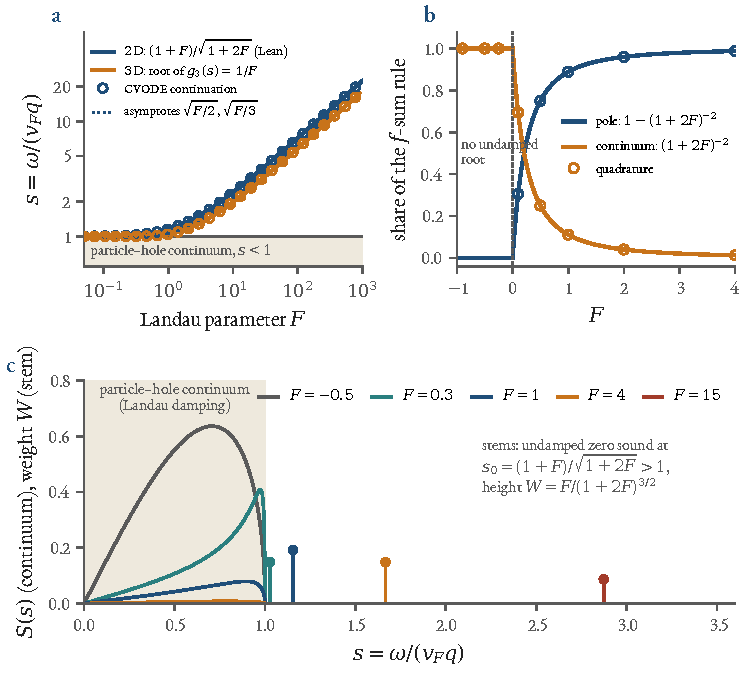
\includegraphics[width=\linewidth]{figures/ch08_zerosound.pdf}
\caption[The zero-sound root and what it carries]{\textbf{The zero-sound root and what it carries.}
\textbf{a}, the root $s(F)$: two dimensions (blue, the Lean closed form), three dimensions (orange, root of $g_3(s)=1/F$); open circles, CVODE continuation of \eqref{ch08:eq-davidenko} ($\ceightV{contPoints}$ points, relative tolerance $\ceightV{contRtol}$); dotted, the asymptotes $\sqrt{F/2}$ and $\sqrt{F/3}$; shaded, the particle--hole continuum $s<1$.
\textbf{b}, shares of the first moment $\int s\hat S\,\dd s=\frac14$: the pole carries $1-(1+2F)^{-2}$ (blue; Lean: \Lthm{ZeroSound2D}{pole_fraction}), the continuum the rest (orange); open circles, quadrature of \eqref{ch08:eq-S}. For $F\le0$ there is no pole.
\textbf{c}, the structure factor \eqref{ch08:eq-S} for five values of $F$ (a curve and its stem have one colour); a stem at $s_0$ has height $W$ of \eqref{ch08:eq-W} and stands for a $\delta$-function.
Script: \texttt{figures/ch08\_zerosound.py}.}\label{ch08:fig-zerosound}
\end{figure}

How much of the spectrum does the line carry?
There is an exact answer.
The function $G(s)=\Omega/(1+F\Omega)$ is analytic in the upper half plane for $F>-1$, and at large $|s|$ one has $\Omega\simeq-1/(2s^2)$, hence $G\simeq-1/(2s^2)$.
Its Hilbert-transform representation $G(s)=\pi^{-1}\!\int\operatorname{Im}G(s')\,(s'-s)^{-1}\dd s'$, with $\operatorname{Im}G$ odd and equal to $\pi\hat S$ for $s>0$, gives $G\simeq-2s^{-2}\int_0^\infty s'\hat S(s')\,\dd s'$, and comparing the two,
\begin{equation}\label{ch08:eq-fsum}
\int_0^\infty s\,\hat S(s)\,\dd s=\frac14\qquad(F>-1),
\end{equation}
which is the $f$-sum rule $\int\omega S\,\dd\omega=nq^2/2m$ of the model (in two dimensions $n=N(0)E_F$ and $E_F=\frac12mv_F^2$).
It holds for every $F$, so a line that exists takes its weight from the band.
The pole contributes $s_0W=F(1+F)/(1+2F)^2$, and since $4F(1+F)=(1+2F)^2-1$ its share is
\begin{equation}\label{ch08:eq-frac}
\frac{s_0W}{1/4}=1-\frac1{(1+2F)^2}\qquad(F>0).
\end{equation}
The identities behind \eqref{ch08:eq-W} and \eqref{ch08:eq-frac} are the new Lean theorems below.
What Lean does \emph{not} prove is that $W$ is the strength of a $\delta$-function in $S$, or that the first moment is $\frac14$: those are the residue theorem and the $f$-sum rule, which the module does not contain.
They are checked numerically: the continuum quadrature plus the pole gives $\frac14$ to $\ceightV{sumDev}$ at eight values of $F$ between $-0.9$ and $15$, and the continuum alone gives $\frac14(1+2F)^{-2}$ for $F>0$ and exactly $\frac14$ for $F\le0$.

\begin{leanbox}{Ch08\_ZeroSound2D (new in this book)}
\begin{lstlisting}[style=lean]
theorem pole_fraction {F : ℝ} (hF : 0 < F) :
    4 * s0 F * (1 / (F ^ 2 * deriv omega2 (s0 F)))
      = 1 - 1 / (1 + 2 * F) ^ 2
\end{lstlisting}
\end{leanbox}

This is \eqref{ch08:eq-frac}, with the residue written $1/(F^2\,\Omega'(s_0))$.
Two further theorems of the new file carry the pieces: \Lthm{ZeroSound2D}{omega2_hasDerivAt} proves $\Omega'(s)=(s^2-1)^{-3/2}$ as a derivative of the function \texttt{omega2}, and \Lthm{ZeroSound2D}{pole_weight} turns that into \eqref{ch08:eq-W}.
The proof of \Lthm{ZeroSound2D}{pole_fraction} is then algebra: the two square roots collapse because $s_0^2-1=F^2/(1+2F)$ (\Lthm{ZeroSound2D}{s0_sq_sub_one}).

Read as physics, \cref{ch08:fig-zerosound}b says that a weak repulsion ($F\to0^+$) gives the line almost no weight, about $4F$ of the sum rule, and leaves it hugging the band, while a strong one pushes it out and gives it almost everything: at $F=4$ the line carries $80/81$.
Whether that says anything about the film the model cannot tell.

%% ====================================================================================================================
\section{Integrating the kinetic equation with CVODE}\label{ch08:sec-cvode}

Equation \eqref{ch08:eq-kinetic} goes onto a computer almost verbatim.
Take units $v_Fq=1$.
For the initial states used below $\nu$ is even in $\theta$, so only $\theta\in(0,\pi)$ is needed, with $N$ midpoint nodes $\theta_j=(j+\tfrac12)\pi/N$ and $\ceightavg{\cdot}\to\frac1N\sum_j$ (a smooth periodic integrand integrated this way is exponentially accurate for times up to order $N$).
With $c_j=\cos\theta_j$ and the real and imaginary parts of $\nu_j$ as unknowns, the system $\dot\nu_j=-\ii c_j(\nu_j+F\ceightavg{\nu})$ is linear with a constant matrix, which is also its Jacobian and is handed to CVODE as such.

\begin{rustbox}{CVODE on the Landau kinetic equation}
Excerpts of the right-hand side and the driver, as run (crate \texttt{cvode} 6.4.0, rusty-SUNDIALS commit \texttt{5db8041}; \texttt{book/rust/ch08\_kinetic}); the closure \texttt{jac} fills the $2N\times2N$ matrix $\left(\begin{smallmatrix}0&A\\-A&0\end{smallmatrix}\right)$, $A_{ij}=c_i\delta_{ij}+c_iF/N$.
\begin{lstlisting}[style=rust]
let rhs = move |_t: f64, y: &[f64], yd: &mut [f64]| -> Result<(), String> {
    let mr = y[..n].iter().sum::<f64>() / nf;
    let mi = y[n..].iter().sum::<f64>() / nf;
    for j in 0..n {
        yd[j] = c_rhs[j] * (y[n + j] + f * mi);
        yd[n + j] = -c_rhs[j] * (y[j] + f * mr);
    }
    Ok(())
};
...
let builder = Cvode::builder(method).rtol(rtol).atol(atol)
    .max_steps(5_000_000);
let builder = if std::env::var("CH08_NOJAC").is_ok() { builder }
    else { builder.jacobian(jac) };
let mut cv = builder.build(rhs, 0.0, SerialVector::from_slice(&y0))
    .expect("build");
...
let (t, y) = cv.solve(tout, Task::Normal)
    .unwrap_or_else(|e| panic!("solve to {tout}: {e:?}"));
\end{lstlisting}
One output ($F=4$, $N=64$, $0\le t\le60$, the density mode $m=\ceightavg\nu$ recorded every $0.1$; the line is the driver's own, copied from \texttt{figures/ch08\_statsline.txt}):
\lstinputlisting[style=plainmono]{figures/ch08_statsline.txt}
Shared eight-core machine, load average 12--35 while these runs were made: wall times are not benchmarks (the same $F=0$ problem took $\ceightV{wallZeroA}$~s and $\ceightV{wallZeroB}$~s in two runs of one batch).
\end{rustbox}

There are exact answers to compare with.
For $F=0$ the nodes decouple and, for the initial state $\nu\equiv1$ (a density wave suddenly released), $m(t)=\ceightavg{\ee^{-\ii t\cos\theta}}=J_0(t)$.
For $F=-\tfrac12$ the Laplace transform of the density is $2/(p+\sqrt{p^2+1})$, whose inverse is $2J_1(t)/t$.
For any $F$ the Laplace transform of $m$ is $\hat m(p)=(p^2+1)^{-1/2}\big/\bigl[1+F\bigl(1-p/\sqrt{p^2+1}\bigr)\bigr]$, which is $\Omega$ continued to imaginary frequency; its singularities are, for $F>0$, the poles $p=\pm\ii s_0$ (residue $F/(1+2F)$ each) and, for every $F$, the cut $|\operatorname{Im}p|<1$ of the square root.
Inverting,
\begin{equation}\label{ch08:eq-uniform}
m(t)=\frac{2F}{1+2F}\cos(s_0t)\;+\;\frac2\pi\int_0^1\frac{(1+F)\sqrt{1-y^2}}{(1+F)^2-(1+2F)y^2}\cos(yt)\,\dd y\qquad(F>0),
\end{equation}
and the same integral alone for $F\le0$; at $t=0$ the two parts are $2F/(1+2F)$ and $1/(1+2F)$ and add to one.
A second initial state, $\nu=\cos\theta$ (a density \emph{kick}), gives a purely imaginary $m$ with $-\operatorname{Im}m(t)/2=\int_0^\infty\hat S(s)\sin(st)\,\dd s$: the time signal is the sine transform of the structure factor \eqref{ch08:eq-S}, the $\delta$-function contributing $W\sin(s_0t)$.
Its slope at $t=0$ is the $f$-sum rule, $\dot m(0)=-\ii\ceightavg{\cos^2\theta}=-\tfrac12\ii$ (the solver's difference quotient over $0.1$ of $\operatorname{Im}m$ is $\ceightV{fsumA}$ at $F=-\frac12$ and $\ceightV{fsumB}$ at $F=12$).

\begin{figure}[tp]
\centering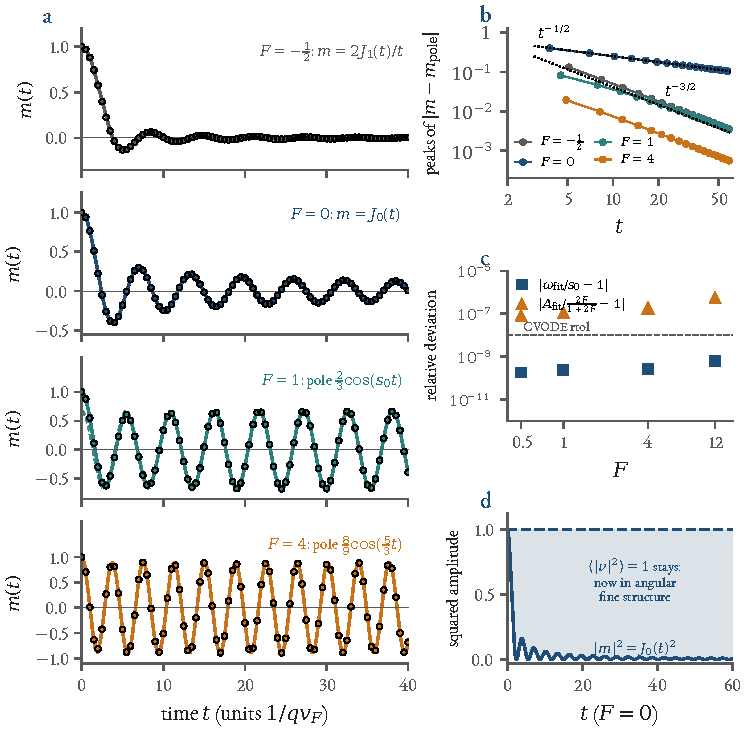
\includegraphics[width=\linewidth]{figures/ch08_timedomain.pdf}
\caption[CVODE against the closed forms of the kinetic equation]{\textbf{CVODE against the closed forms.} Units $v_Fq=1$, BDF, $N=64$, relative tolerance $10^{-8}$.
\textbf{a}, the density amplitude $m(t)$ after a released density wave, for $F=-\frac12$ (exactly $2J_1(t)/t$), $F=0$ ($J_0(t)$), $F=1$ and $F=4$ (the sum \eqref{ch08:eq-uniform} of an undamped line, dashed, and a band that dephases); open circles, CVODE every $0.5$ time units; lines, closed forms.
\textbf{b}, peaks of the part of $m$ that is not the pole: the band's contribution decays algebraically, as $t^{-1/2}$ at $F=0$ and $t^{-3/2}$ otherwise.
\textbf{c}, deviation of the fitted late-time frequency from the Lean root $s_0$ (blue) and of the fitted amplitude from $2F/(1+2F)$ (orange), after the exactly known band part has been subtracted.
\textbf{d}, $F=0$: the squared density amplitude (solid) against the squared norm of the Fermi-circle distortion (dashed); the shading is the part of the distortion no longer visible in the density.
Script: \texttt{figures/ch08\_timedomain.py}.}\label{ch08:fig-timedomain}
\end{figure}

\Cref{ch08:fig-timedomain}a is that formula made visible, and \cref{ch08:tab-solver} gives the numbers.
CVODE agrees with the closed forms at every $F$ tried: the largest deviation over $0\le t\le60$ is $\ceightV{errU_m0p5}$ at $F=-\frac12$ and $\ceightV{errU_0}$ at $F=0$, and grows to $\ceightV{errU_12}$ at $F=12$, where the solution oscillates fastest and more steps accumulate more error; for the kick the deviations of $-\operatorname{Im}m/2$ from the sine transform are $\ceightV{errK_m0p5}$ and $\ceightV{errK_12}$.

The sharpest test against Lean is the pole.
Subtract the exactly known band part of \eqref{ch08:eq-uniform} from the CVODE signal; what remains must be one undamped cosine.
A least-squares fit of $A\cos(\omega t+\varphi)$ over $0\le t\le60$ gives, at $F=4$, $\omega=\ceightV{omegaFit4}$ against the Lean root $s_0=5/3=1.666666667$ and $A=\ceightV{ampFit4}$ against $2F/(1+2F)=8/9$; at $F=\frac12$, $\omega=\ceightV{omegaFit05}$ against $s_0=\ceightV{sZeroHalf}$.
Over $F=\frac12,1,4,12$ the frequency agrees with $s_0$ to a relative $\ceightV{fitW_0p5}$ to $\ceightV{fitW_12}$ and the amplitude with $2F/(1+2F)$ to $\ceightV{fitA_0p5}$ to $\ceightV{fitA_12}$ (\cref{ch08:fig-timedomain}c).
The time integration of the kinetic equation lands on the number that Lean proved to exist, ten digits deep.

\begin{table}[tp]
\centering\small
\caption{\textbf{CVODE (BDF, $N=64$, relative tolerance $10^{-8}$, absolute $10^{-10}$) on the kinetic equation, $0\le t\le60$, against the closed forms.} ``Released'': $\nu\equiv1$; ``kick'': $\nu=\cos\theta$ (not run at $F=0$). Energy drift: $\max_t|E(t)/E(0)-1|$ for the conserved form \eqref{ch08:eq-energy}. Steps for the released runs.}\label{ch08:tab-solver}
\begin{tabular}{@{}r@{\quad}c@{\quad}c@{\quad}c@{\quad}r@{}}
\toprule
$F$ & max error, released & max error, kick & energy drift & steps\\
\midrule
$-\tfrac12$ & \ceightV{errU_m0p5} & \ceightV{errK_m0p5} & \ceightV{edrift_m0p5} & \ceightV{stepsU_m0p5}\\
$0$ & \ceightV{errU_0} & --- & \ceightV{edrift_0} & \ceightV{stepsU_0}\\
$\tfrac12$ & \ceightV{errU_0p5} & \ceightV{errK_0p5} & \ceightV{edrift_0p5} & \ceightV{stepsU_0p5}\\
$1$ & \ceightV{errU_1} & \ceightV{errK_1} & \ceightV{edrift_1} & \ceightV{stepsU_1}\\
$4$ & \ceightV{errU_4} & \ceightV{errK_4} & \ceightV{edrift_4} & \ceightV{stepsU_4}\\
$12$ & \ceightV{errU_12} & \ceightV{errK_12} & \ceightV{edrift_12} & \ceightV{stepsU_12}\\
\bottomrule
\end{tabular}
\end{table}

Two choices about the solver were not free, and a reader reproducing this should know them.
\emph{BDF, not Adams.}
At $F=0$, $N=64$, output every $0.1$, the BDF option reproduces $J_0$ to $\ceightV{tol_bdf_06}$, $\ceightV{tol_bdf_08}$ and $\ceightV{tol_bdf_10}$ at relative tolerances $10^{-6}$, $10^{-8}$, $10^{-10}$; the Adams option of the same crate gives $\ceightV{tol_adams_06}$, $\ceightV{tol_adams_08}$ and $\ceightV{tol_adams_10}$, the first two of the order of the signal itself or larger.
The defect is intermittent.
With only $N=4$ nodes at tolerance $10^{-8}$, Adams is accurate ($\ceightV{sweepAdamsGoodMin}$ to $\ceightV{sweepAdamsGoodMax}$) when the solution is requested every $0.01$, $1$, $5$, $10$, $20$ or $60$ time units, and wrong ($\ceightV{sweepAdamsBad}$; $\ceightV{sweepAdamsBadFD}$ with the Jacobian differenced by CVODE) when it is requested every $0.1$, while BDF stays between $\ceightV{sweepBdfMin}$ and $\ceightV{sweepBdfMax}$ for all seven spacings.
We did not look for the cause; the chapter's runs use BDF.
\emph{The crate, not the installed Python module.}
The module \texttt{rusty\_sundials} in the book's virtual environment (file dated \ceightV{modStaleDate}, the day before the repository's tight-tolerance fix) fails on this system at tolerances $10^{-8}$ and $10^{-10}$ (``too many error test failures at one step''), and its Adams option converges only as the square root of the tolerance, the signature of a first-order method ($\ceightV{mod_stale_adams_06}$, $\ceightV{mod_stale_adams_08}$, $\ceightV{mod_stale_adams_10}$ for $N=32$ to $t=0.5$); a build of commit \texttt{\ceightV{modFreshCommit}} passes the same test with either method (errors $\ceightV{mod_fresh_bdf_06}$ to $\ceightV{mod_fresh_bdf_10}$ for BDF, $\ceightV{mod_fresh_adams_06}$ to $\ceightV{mod_fresh_adams_10}$ for Adams).
Everything in this chapter was computed with the Rust crates directly, at that commit.
Last, $N=96$ instead of $64$ at $F=4$ changes the result by $\ceightV{nNinetySix}$, within tolerance, with $\ceightV{stepsN96}$ steps against $\ceightV{stepsN64}$.

%% ====================================================================================================================
\section{Landau damping is dephasing}\label{ch08:sec-dephasing}

At $F=0$, \cref{ch08:fig-timedomain}a shows a density that dies out, $m=J_0(t)\to0$, in a system without any dissipation.
Where did it go?
The equation \eqref{ch08:eq-kinetic} conserves the quadratic form
\begin{equation}\label{ch08:eq-energy}
E=\ceightavg{|\nu|^2}+F\,|\ceightavg{\nu}|^2 ,\qquad \frac{\dd E}{\dd t}=0 .
\end{equation}
At $F=0$ this is the squared norm of the Fermi-circle distortion, and $\ceightavg{|\nu|^2}=1$ for all time (the solver keeps it to $\ceightV{normDrift}$ up to $t=60$) while $|m|^2=J_0(t)^2$ has fallen to $\ceightV{mSqEnd}$ (\cref{ch08:fig-timedomain}d).
The amplitude of the distortion is intact; it has moved from the angular average, which the density sees, into angular structure of ever finer scale.
Landau damping is dephasing, not dissipation: each direction oscillates at its own frequency $v_Fq\cos\theta$, and the average over directions loses coherence.

\Cref{ch08:fig-fermisurface} shows it directly.
It plots the Fermi circle itself, $r=1+\epsilon\operatorname{Re}\nu(\theta,t)$, at the place where the density wave has its maximum, for $F=0$ and $F=4$ (the profile on a fine angular grid is reconstructed from the CVODE solution by the exact Duhamel formula $\nu=\ee^{-\ii ct}\bigl[\nu_0-\ii Fc\int_0^t\ee^{\ii ct'}m(t')\,\dd t'\bigr]$, $c=\cos\theta$, and agrees with the solver's node values to $\ceightV{reconF0}$ and $\ceightV{reconF4}$).
At $F=0$ the ripples multiply in proportion to $t$, because the phase $t\cos\theta$ changes with $\theta$ at the rate $t\sin\theta$; near $\theta=0$ and $\pi$ it does not change, to first order.
Those are the quasi-particles that move along the wave vector at the speed of the wave: they do not dephase, and they are the resonance of \cref{ch08:sec-model}.
At $F=4$ the same filaments are present and, on top of them, a large smooth distortion of the circle, flattened at $\theta=0,\pi$ and bulging at $\pm\pi/2$ at one moment and the reverse half a period later: zero sound, a collective mode of the whole circle, with a maximum $|\nu|$ of $\ceightV{nuMaxFour12}$ at $t=12$.

\begin{figure}[tp]
\centering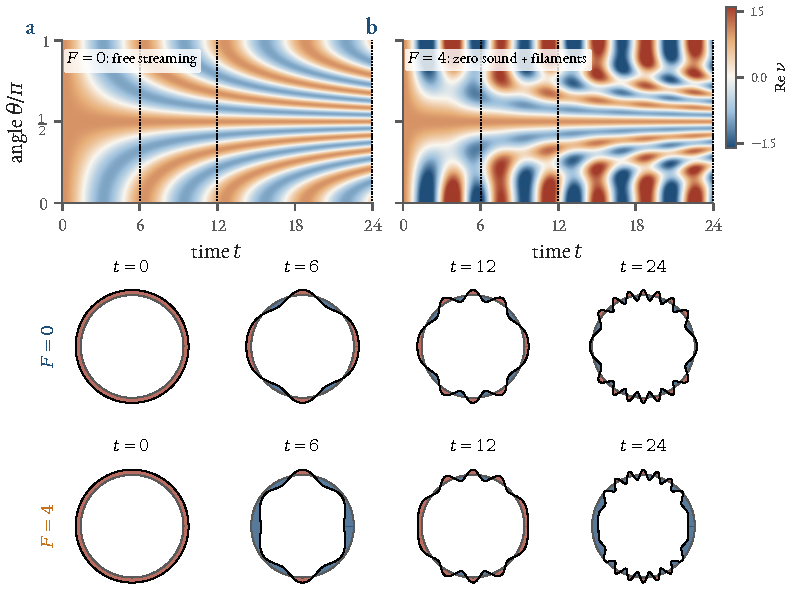
\includegraphics[width=\linewidth]{figures/ch08_fermisurface.pdf}
\caption[The Fermi circle as the dynamical variable]{\textbf{The Fermi circle as the dynamical variable.}
Top: $\operatorname{Re}\nu(\theta,t)$ after a released density wave, $F=0$ (free streaming: a fan of stripes, pitch shrinking as $1/t$ except at $\theta=0,\pi$) and $F=4$ (zero sound at $s_0=5/3$: large smooth lobes near $\theta=0$ and $\pi$ on top of the same fan); the colour scale saturates at $\pm1.6$.
Below: the circle $r=1+\epsilon\operatorname{Re}\nu$, $\epsilon=\ceightV{epsFS}$ (deformation magnified, the same $\epsilon$ in every panel; red outward, blue inward) at $t=0,6,12,24$; the wave vector points to the right.
At $F=0$ the circle keeps $\ceightavg{|\nu|^2}=1$ while the density average decays: the amplitude has moved into the ripples.
Script: \texttt{figures/ch08\_fermisurface.py}.}\label{ch08:fig-fermisurface}
\end{figure}

The decay law of what is left in the density comes from the edge of the continuum.
The part of $m$ that is not the pole is the cosine transform of a spectral density that vanishes like $(1-y)^{1/2}$ at the edge $y=1$ for every $F\ne0$, and diverges like $(1-y)^{-1/2}$ at $F=0$, where the denominator in \eqref{ch08:eq-uniform} vanishes at $y=1$; the transforms decay as $t^{-3/2}$ and $t^{-1/2}$.
The solver reproduces both: the fitted slopes of the envelope of the non-pole part over $10\le t\le60$ are $\ceightV{expo_0}$ at $F=0$ and $\ceightV{expo_m0p5}$ at $F=-\frac12$ (\cref{ch08:fig-timedomain}b), and $\ceightV{expo_4}$ at $F=4$; at $F=1$, where the asymptotics sets in later, it is $\ceightV{expo_1}$ in this window.

The library holds the field-free core of this picture.
The module \texttt{PhaseMixing} proves, with no regularity assumed, that the $k$-th density mode of free transport $\ee^{\ii k(x-vt)}g(v)$ tends to zero (\Lthm{PhaseMixing}{phase_mixing}, an application of the Riemann--Lebesgue lemma), and that for the unit Maxwellian it is exactly $\ee^{-k^2t^2/2}$ (\Lthm{PhaseMixing}{maxwellian_mode}, quoted in \cref{ch08:sec-vlasov}); for the circle the analogue is $J_0$, which is not in the library.
That module is subsumed by Bedrossian's Lean formalisation of the nonlinear Mouhot--Villani theorem \cite{MouhotVillani2011,Bedrossian2026} and claims nothing beyond the linear statement.

Finally, \eqref{ch08:eq-energy} is the energy of the Pomeranchuk bound.
Because $|\ceightavg\nu|^2\le\ceightavg{|\nu|^2}$, one has $E\ge\min(1,1+F)\ceightavg{|\nu|^2}$: for $F>-1$ the form is positive definite and every solution of the single-wave model stays bounded.
Below the bound it is indefinite and the model has a growing solution: with $s=\ii y$, \eqref{ch08:eq-disp} reads $1+F\bigl(1-y/\sqrt{1+y^2}\bigr)=0$, solved by $y=r/\sqrt{1-r^2}$, $r=1-1/|F|$, once $F<-1$; at $F=-2$, $y=1/\sqrt3=\ceightV{growthPred}$.
CVODE at $F=-2$ grows as $\ee^{yt}$ with the fitted rate $\ceightV{growthFit}$ over $10\le t\le14$, $E$ conserved to $\ceightV{growthEdrift}$.
This is a simulation of an elementary instability, not a theorem: the library contains no stability theorem for the Landau equation (\cref{ch08:honest}, item 3).

%% ====================================================================================================================
\section{A plasma cousin, and the property that decides}\label{ch08:sec-vlasov}

Equation \eqref{ch08:eq-kinetic} resembles the Vlasov equation of a plasma, and the rusty-SUNDIALS repository has a solver for one: the crate \texttt{qf-vlasov1d}, one space and one velocity dimension, electrons on a neutralising background (units of the plasma frequency),
\begin{equation}\label{ch08:eq-vlasov}
\partial_tf+v\,\partial_xf-E\,\partial_vf=0,\qquad \partial_xE=1-\!\int\! f\,\dd v .
\end{equation}
It advances $x$ by an exact Fourier shift and $v$ by a cubic semi-Lagrangian step (a natural spline, a documented departure from its Python original), in Strang splitting, on $32\times512$ cells with $|v|\le6$ and time step $0.1$.
Two backgrounds $f_0(v)$ of equal density are used: a Maxwellian, and a degenerate Fermi--Dirac profile $f_0\propto[1+\ee^{(|v|-v_0)/w}]^{-1}$ with $v_0=1$, $w=0.1$, a sea with two smeared edges that is the one-dimensional Fermi surface.
The Maxwellian is perturbed in density, $f_0(1+a\cos kx)$; the degenerate sea by displacing its edges, $v_0\to v_0(1+a\cos kx)$, so that the perturbation lives where a Fermi gas can have one.

\begin{rustbox}{qf-vlasov1d on two backgrounds}
From the driver \texttt{book/rust/ch08\_vlasov}: the two backgrounds on the velocity grid, and the evolution (excerpt).
\begin{lstlisting}[style=rust]
Bg::Maxwell => maxwellian(v, 0.0),
Bg::Fermi { v0, w } => 1.0 / (1.0 + ((v.abs() - v0) / w).exp()),
...
let g = Grid::new(2.0 * PI / k, 32, nv, 6.0);
let f0 = initial(&g, bg, a);
run(f0, &g, dt, t_end, observe, field_on,
    Vec::<(f64, fn(&[f64]) -> Vec<f64>)>::new());
\end{lstlisting}
\end{rustbox}

The linear theory is a dispersion relation of the type \eqref{ch08:eq-disp}: $1-k^{-2}\int f_0'(v)\,(v-\omega/k)^{-1}\dd v=0$ along Landau's contour.
For the Maxwellian it is the textbook relation with the plasma dispersion function; at $k=\tfrac12$ it has the root $\omega=\ceightV{vmCertRe}-\ceightV{vmCertIm}\,\ii$ (our mpmath calculation), which agrees with the programme's certified root of its earlier kinetic benchmark ($\ceightV{vmProgRe}-\ceightV{vmProgIm}\,\ii$ to the digits printed) to $\ceightV{vmCertDiff}$.
\Cref{ch08:fig-vlasov} shows both runs.
With the Maxwellian the density perturbation is sheared into filaments of ever finer velocity structure, pitch $2\pi/(kt)$, and the field decays as $\ee^{\gamma t}$ with $\gamma=-\ceightV{vmG_0p5}$.
With the degenerate sea the same density wave rides on the two Fermi edges and does not decay.
Least-squares fits of the solver's signed density mode over $5\le t\le40$ (amplitude, rate, frequency and phase free) give \cref{ch08:tab-vlasov}: for the Maxwellian the rates agree with the roots within $\ceightV{vmRelG_0p3}$ at $k=0.3$, where the mode has lost only $\ceightV{vmLost03}$ of its amplitude by $t=40$, and to better than $\ceightV{vmRelG_0p5}$ from $k=\tfrac12$ up, with frequencies within $\ceightV{vmRelW_0p4}$; going from $n_v=128$ to $256$ to $512$ moves the fitted rates by at most $\ceightV{vmConvMax}$.

\begin{table}[tp]
\centering\small
\caption{\textbf{qf-vlasov1d against linear theory} ($k$ in inverse Debye lengths; $n_v=512$): fits of the signed density mode over $5\le t\le40$ (Maxwellian: the window ends when the mode falls below $3\times10^{-5}$ of its maximum) and the degenerate profile $v_0=1$, $w=0.1$. Degenerate theory: continued root at $k=0.5,\,0.8$, weak-damping formula at $k=0.3$. Rates below about $10^{-4}$ are at the resolution of the fit (residual $\ceightV{vfRes_0p5}$ of the signal at $k=0.5$).}\label{ch08:tab-vlasov}
\begin{tabular}{@{}l@{\quad}c@{\quad}c@{\quad}c@{\quad}c@{\quad}c@{\quad}c@{}}
\toprule
 & $k$ & $\omega_{\rm theory}$ & $\omega_{\rm solver}$ & $|\gamma|_{\rm theory}$ & $|\gamma|_{\rm solver}$ & rel.\ diff.\ $\gamma$\\
\midrule
Maxwellian & 0.3 & \ceightV{vmW_0p3} & \ceightV{vmWs_0p3} & \ceightV{vmG_0p3} & \ceightV{vmGs_0p3} & \ceightV{vmRelG_0p3}\\
 & 0.5 & \ceightV{vmW_0p5} & \ceightV{vmWs_0p5} & \ceightV{vmG_0p5} & \ceightV{vmGs_0p5} & \ceightV{vmRelG_0p5}\\
 & 0.8 & \ceightV{vmW_0p8} & \ceightV{vmWs_0p8} & \ceightV{vmG_0p8} & \ceightV{vmGs_0p8} & \ceightV{vmRelG_0p8}\\
\midrule
degenerate & 0.3 & \ceightV{vfW_0p3} & \ceightV{vfWs_0p3} & \ceightV{vfG_0p3} & \ceightV{vfGs_0p3} & ---\\
 & 0.5 & \ceightV{vfW_0p5} & \ceightV{vfWs_0p5} & \ceightV{vfG_0p5} & \ceightV{vfGs_0p5} & ---\\
 & 0.8 & \ceightV{vfW_0p8} & \ceightV{vfWs_0p8} & \ceightV{vfG_0p8} & \ceightV{vfGs_0p8} & \ceightV{vfRelG_0p8}\\
\bottomrule
\end{tabular}
\end{table}

\begin{figure}[tp]
\centering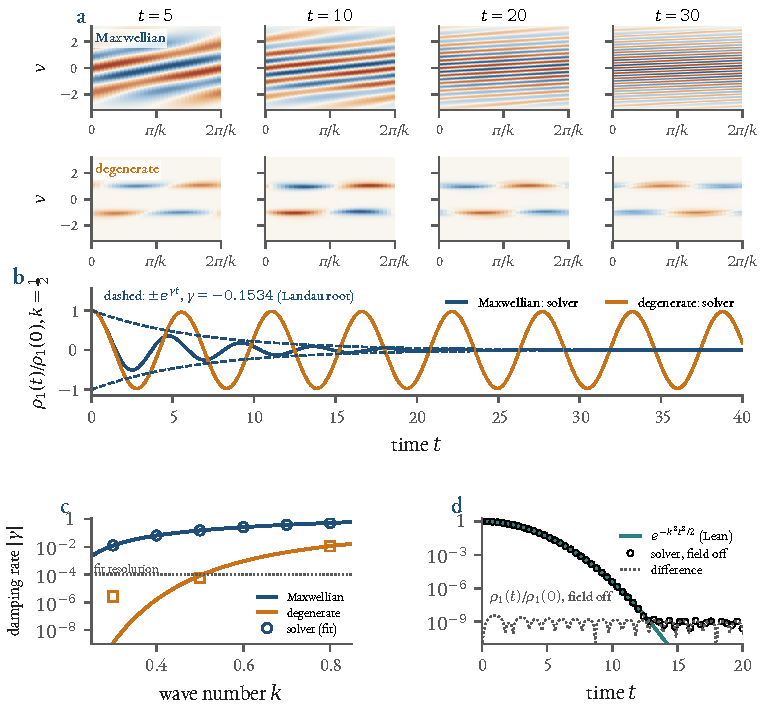
\includegraphics[width=\linewidth]{figures/ch08_vlasov.pdf}
\caption[Vlasov--Poisson: the same density wave on two backgrounds]{\textbf{Vlasov--Poisson (\texttt{qf-vlasov1d}): the same density wave on two backgrounds.}
\textbf{a}, the perturbation $f(x,v,t)-\bar f_0(v)$ at $k=\frac12$, $a=0.05$, $t=5,10,20,30$ (colour scale per row): for the Maxwellian (top) filaments of velocity pitch $2\pi/kt$; for the degenerate sea (bottom) a pair of edge waves.
\textbf{b}, the density mode $\rho_1(t)/\rho_1(0)$ at $k=\frac12$, $a=0.01$: damped (blue; dashed, the envelope $\pm\ee^{\gamma t}$ with the Landau root) and undamped (orange).
\textbf{c}, damping rate against $k$: linear theory (lines) and solver fits (symbols); the degenerate curve is the weak-damping formula, and solver rates below about $10^{-4}$ are at the resolution of the fit.
\textbf{d}, the field-off control: the density mode of free streaming (circles) against $\ee^{-k^2t^2/2}$ (line; Lean: \Lthm{PhaseMixing}{maxwellian_mode}); dotted, the difference, at the floor set by cutting the Maxwellian at $|v|=6$.
Script: \texttt{figures/ch08\_vlasov.py}.}\label{ch08:fig-vlasov}
\end{figure}

The degenerate background tells the other half.
Its roots are $\omega=\ceightV{vfW_0p3}$, $\ceightV{vfW_0p5}$, $\ceightV{vfW_0p8}$ at $k=0.3,\,0.5,\,0.8$, with damping rates $\ceightV{vfG_0p3}$, $\ceightV{vfG_0p5}$ and $\ceightV{vfG_0p8}$: exponentially small at small $k$ because the phase velocity $\omega/k$ lies several widths $w$ beyond the edge $v_0$, where the resonant fraction is $\sim\ee^{-(\omega/k-v_0)/w}$.
The solver's frequencies are $\ceightV{vfWs_0p3}$, $\ceightV{vfWs_0p5}$, $\ceightV{vfWs_0p8}$, and its damping rate at $k=0.8$, large enough to measure, is $\ceightV{vfGs_0p8}$ against $\ceightV{vfG_0p8}$.
At $k=0.3$ and $0.5$ the true rates are below the resolution of the fit; what the solver supports is $|\gamma|<10^{-4}$, three orders of magnitude below the Maxwellian $\ceightV{vmG_0p5}$ at $k=\tfrac12$.
The field-off control is the Lean statement in numbers: with the field switched off, the density mode of the Maxwellian run is $\ee^{-k^2t^2/2}$ to $\ceightV{fsMax}$ over $0\le t\le40$, down to a floor of $\ceightV{fsFloor}$ set by the cut at $|v|=6$, and the free-streaming recurrence, an artefact of any velocity grid at $t=2\pi/(k\,\Delta v)=\ceightV{fsRecur}$, is far outside the window.

\begin{leanbox}[unbreakable]{PhaseMixing}
\begin{lstlisting}[style=lean]
theorem maxwellian_mode (k t : ℝ) :
    ∫ v : ℝ, cexp (-((k * v * t : ℝ) : ℂ) * I) *
        ((rexp (-v ^ 2 / 2) / √(2 * π) : ℝ) : ℂ)
      = cexp (-((k * t) ^ 2 / 2 : ℝ))
\end{lstlisting}
\end{leanbox}

\begin{keybox}[An analogy is not a result]
The finding is ``a collective mode of a collisionless kinetic equation is damped by phase mixing''.
The tempting transfer: the plasma shows Landau damping, so Fermi-liquid zero sound is Landau damped.
What the finding depends on is not the form of the equation, which the two systems share, but the \emph{support} of the velocity distribution relative to the phase velocity of the wave.
A Maxwellian has unbounded support, so some particles always move at the phase velocity and the mode is damped at a rate fixed by $f_0'(\omega/k)$; a degenerate gas has bounded support, and a wave faster than the edge has no resonant particles.
The degenerate run shows precisely this, and a Fermi circle has the property: $s>1$ in \eqref{ch08:eq-disp} is its statement.
What does \emph{not} transfer is any number: the plasma's interaction is a long-range force of strength $1/k^2$ where the Fermi liquid has the contact parameter $F$, the roots solve different equations, and the rate $\ceightV{vmG_0p5}$ is a fact about electrons on a Maxwellian background and nothing about helium.
\end{keybox}

%% ====================================================================================================================
\section{Beyond Landau: the window at twice the Fermi momentum}\label{ch08:sec-window}

\begin{figure}[tp]
\centering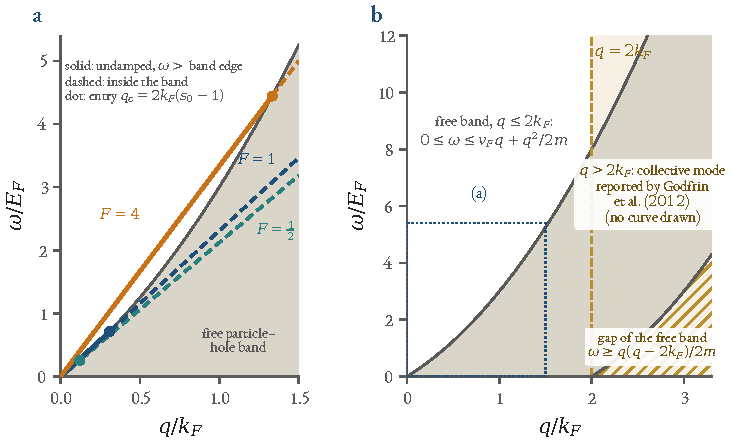
\includegraphics[width=\linewidth]{figures/ch08_window.pdf}
\caption[The $(q,\omega)$ plane in free-gas units]{\textbf{The $(q,\omega)$ plane, in free-gas units} ($q/k_F$, $\omega/E_F$ with $E_F=\hbar^2k_F^2/2m$, so that $v_Fq=2(q/k_F)E_F$).
\textbf{a}, the Landau line $\omega=s_0v_Fq$ for $F=\frac12,1,4$ against the upper edge $v_Fq+\hbar q^2/2m$ of the free particle--hole band (grey): solid where the line is above the edge (undamped), dashed once inside (damped), dot at the entry $q_c=2k_F(s_0-1)$.
\textbf{b}, the whole free band up to $3.3\,k_F$: its lower edge is $0$ for $q\le2k_F$ and $\hbar q(q-2k_F)/2m$ for $q>2k_F$ (hatched, the gap; Lean: \Lthm{ZeroSound2D}{ph_gap}); gold, the momentum transfers $q>2k_F$ at which Godfrin \emph{et al.}\ report the reappearing collective mode.
No curve is drawn there.
Script: \texttt{figures/ch08\_window.py}.}\label{ch08:fig-window}
\end{figure}

What does the model say about the third regime of \cref{ch08:sec-measure}?
Nothing, and it is worth seeing why.
The model's collective mode is the straight line $\omega=s_0v_Fq$, derived for $q\ll k_F$ with a single parameter $F$ and no scale at which a minimum could form.
Against the free-gas band of \cref{ch08:fig-window}a the line enters the edge $v_Fq+\hbar q^2/2m$ at $q_c=2k_F(s_0-1)$, which is $\ceightV{qc_0p5}\,k_F$ at $F=\frac12$, $\ceightV{qc_1}\,k_F$ at $F=1$, $\ceightV{qc_4}\,k_F$ at $F=4$ and $\ceightV{qc_12}\,k_F$ at $F=12$ (for $F\ge3+2\sqrt3=\ceightV{Fstar}$ it stays above the edge up to $q=2k_F$); beyond $q_c$ the model's answer is a broadened line.
That is the second regime of the abstracts, in outline: the zero-sound mode enters the band and is damped.
It is not a quantitative claim about the film, whose $F$, effective mass and $k_F$ are not known here; and for the larger values of $F$ the entry point is at $q_c\gtrsim k_F$, outside the range $q\ll k_F$ for which the straight line was derived.

The one exact statement about the third regime that survives in this framework is kinematic and holds for the free gas: the band has a lower edge, and the edge lifts off $\omega=0$ at $q=2k_F$.

\begin{leanbox}{Ch08\_ZeroSound2D (new in this book)}
\begin{lstlisting}[style=lean]
theorem ph_gap {E : Type*} [NormedAddCommGroup E]
    [InnerProductSpace ℝ E] {m kF : ℝ} (hm : 0 < m)
    (hkF : 0 ≤ kF) (k q : E) (hk : ‖k‖ ≤ kF)
    (hq : 2 * kF < ‖q‖) :
    0 < ‖q‖ * (‖q‖ - 2 * kF) / (2 * m) ∧
      ‖q‖ * (‖q‖ - 2 * kF) / (2 * m)
        ≤ (‖k + q‖ ^ 2 - ‖k‖ ^ 2) / (2 * m)
\end{lstlisting}
\end{leanbox}

A hole of momentum $k$ inside the Fermi sphere ($\|k\|\le k_F$) and a particle of momentum $k+q$ cost the energy $(\|k+q\|^2-\|k\|^2)/2m$ (with $\hbar=1$).
The gap theorem says that for $q>2k_F$ every such pair costs at least $q(q-2k_F)/2m>0$.
It rests on \Lthm{ZeroSound2D}{ph_energy_window}, which puts the cost between $(q^2-2k_Fq)/2m$ and $(q^2+2k_Fq)/2m$ in \emph{any} real inner-product space, hence for the film and for the bulk liquid alike; the proof is the Cauchy--Schwarz inequality $|\langle k,q\rangle|\le k_Fq$ and nothing else.
And \Lthm{ZeroSound2D}{ph_edge_attained} says the lower bound is reached, by the hole $k=-(k_F/\|q\|)\,q$ on the Fermi surface, whose partner $k+q$ lies outside it as soon as $\|q\|\ge2k_F$.
For $q<2k_F$ the lower edge is zero, because the bound is negative and a pair at the Fermi surface can cost arbitrarily little.

This is the mathematics of the number $2k_F$ in the 2012 abstract: the collective mode is said to reappear at momentum transfers larger than twice the Fermi momentum, and $2k_F$ is where the free band opens a window below itself.
The coincidence is noted; it is not claimed as the explanation.
The abstracts say that the reappearing excitation lies ``beyond the particle-hole band'', with a dispersion ``quite similar to that of superfluid $^4$He'', and that a dynamic many-body theory interprets the spectra.
Whether the observed mode sits in the free band's window, how the interaction pushes it, and why it has a minimum are exactly what a theory of pair fluctuations beyond the Landau parameter must answer, and what this book's tools do not reach; the Godfrin--Krotscheck survey \cite{GodfrinKrotscheck2022} is the place to read how the question is treated.
In the helium-4 chapters the roton is a feature of a measured curve (\cref{ch05}); here it is a feature that a measurement found in a system where the standard theory did not expect it.

%% ====================================================================================================================
\section{What is established, and what is not}\label{ch08:honest}

\begin{honestbox}
\textbf{Proved (Lean, standard axioms only).} The library: \Lthm{ZeroSound}{zero_sound_2d_iff} and \Lthm{ZeroSound}{zero_sound_iff} (an undamped zero-sound root $s>1$ exists iff $F>0$; 2D with the explicit root, 3D by pinning and the intermediate value theorem) and \Lthm{PhaseMixing}{maxwellian_mode}.
New in this book, in \texttt{book/lean/Ch08\_ZeroSound2D.lean} (namespace \texttt{QuantumFluids.ZeroSound2D}): uniqueness of the 2D root, the derivative of $\Omega_{2\mathrm D}$, the residue weight and its share of the first moment, and the free-gas particle--hole window.
The file compiles with the pinned Lean 4 and Mathlib with no \texttt{sorry}; \texttt{\#print axioms} reports \ceightV{leanAxioms} for each of its nine theorems.
These are statements about mathematics; that a helium film obeys them is physics.\par\vspace{3pt}
\textbf{Derived and checked numerically, not in Lean.} The structure factor \eqref{ch08:eq-S}; the residue as the strength of a $\delta$-function; the $f$-sum rule \eqref{ch08:eq-fsum} (the quadrature closes it to $\ceightV{sumDev}$); the exact solutions $J_0$ and $2J_1(t)/t$ and the formula \eqref{ch08:eq-uniform}; the conserved form \eqref{ch08:eq-energy}.\par\vspace{3pt}
\textbf{Simulated.} CVODE (BDF) on the kinetic equation (errors $\ceightV{errU_m0p5}$ to $\ceightV{errU_12}$ against the closed forms) and on the root continuation; \texttt{qf-vlasov1d}.\par\vspace{3pt}
\textbf{Measured, by others.} Everything about helium, by Godfrin and his collaborators \cite{Godfrin2010,Godfrin2012}, quoted from their abstracts.
This book has no spectra and no film parameters; every number here is a function of the free $F$.\par\vspace{3pt}
\textbf{Only an analogy.} Plasma against Fermi liquid.
What they share (free streaming plus a mean field, dephasing) is real, and the degenerate run confirms the property that decides whether a mode is damped (bounded support); the plasma's numbers say nothing about helium.\par\vspace{3pt}
\textbf{Not claimed, and not possible here.} The roton; any finite-$q$ or finite-temperature statement; $F_1^s$ and the effective mass; collisions and the crossover from zero to first sound; a comparison with the film.
Past the line the model draws, the chapter says only what is free-gas kinematics.\par\vspace{3pt}
\textbf{What failed or was withdrawn.}
(1) The installed Python module of CVODE failed on this problem, and the Adams option of the crate gave wrong answers at one output spacing (\cref{ch08:sec-cvode}); reported, not investigated.
(2) A first estimate of the Vlasov damping rates from the spacing of field maxima returned a positive rate for the weakly damped degenerate run ($+\ceightV{peakFitFermi05}$ at $k=0.5$); it was replaced by least-squares fits, and rates below about $10^{-4}$ are not claimed.
(3) The programme's attempt to formalise a Pomeranchuk--Penrose stability theorem for the 2D Landau equation was stopped at its literature gate (CLAIM-030); the library has none.
(4) The programme's two searches for the 2D Landau parameters of the film found no open table (CLAIM-030, CLAIM-031); the ledger names the 2010 paper as a likely source, and only its abstract, which gives no parameter, was read for this chapter.
\end{honestbox}

%% ====================================================================================================================
\section*{Exercises}

\paragraph{Exercise 1.}
Show that squaring $1+F\,\Omega_{2\mathrm D}(s)=0$ gives $s^2(1+2F)=(1+F)^2$, and that the positive root solves the unsquared equation exactly when $F>0$.
Expand $s_0$ for small $F$ to order $F^3$ and verify $s_0^2=\frac F2+\frac34+\frac1{4(1+2F)}$.
\emph{Hint.} $(1+F)^2-F^2=1+2F$; the unsquared equation needs $Fs/(1+F)>0$, which is where the sign of $F$ enters. Answer: $s_0-1=F^2/2-F^3+O(F^4)$.

\paragraph{Exercise 2.}
Derive \eqref{ch08:eq-W} from $\Omega'(s)=(s^2-1)^{-3/2}$ and \eqref{ch08:eq-root}, then \eqref{ch08:eq-frac}.
For which $F$ does the zero-sound line carry $90\,\%$ of the first moment?
Show also that \eqref{ch08:eq-fsum} follows from $G(s)\simeq-1/(2s^2)$ at large $|s|$.
\emph{Hint.} $s_0W=F(1+F)/(1+2F)^2$ and $4F(1+F)=(1+2F)^2-1$; the first answer is $(1+2F)^2=10$, i.e.\ $F=(\sqrt{10}-1)/2=\ceightV{Fninety}$.

\paragraph{Exercise 3.}
Prove that $E=\ceightavg{|\nu|^2}+F|\ceightavg\nu|^2$ is constant along solutions of \eqref{ch08:eq-kinetic} for a single wave vector, and that for $F>-1$ every solution is bounded.
Then find the growth rate for $F<-1$ and compare it with the CVODE run at $F=-2$ of \cref{ch08:sec-dephasing}.
\emph{Hint.} Differentiate both terms: only the cross terms $\pm2F\operatorname{Re}[\ii\,m^*\ceightavg{\cos\theta\,\nu}]$ survive, and they cancel; $\ceightavg{\cos\theta}=0$ removes the $Fm$ term from $\dot m$. For the rate put $s=\ii y$ and use $\ceightavg{(\cos^2\theta+y^2)^{-1}}=1/(y\sqrt{1+y^2})$.

%% ====================================================================================================================
\section*{Notes and further reading}

Landau's theory of the Fermi liquid is in his 1957 paper \cite{Landau1957}; its textbook presentation, with the kinetic equation, the Landau parameters and zero sound, is Baym and Pethick \cite{BaymPethick1991}.
Zero sound was observed in liquid $^3$He by Abel, Anderson and Wheatley in 1966 \cite{AbelAndersonWheatley1966}.
The measurements this chapter is organised around are \cite{Godfrin2010,Godfrin2012}, and the Godfrin--Krotscheck survey of excitation spectra of quantum fluids \cite{GodfrinKrotscheck2022} puts them in context.
Landau damping as a theorem (nonlinear, Vlasov--Poisson) is due to Mouhot and Villani \cite{MouhotVillani2011}, its Lean 4 formalisation to Bedrossian \cite{Bedrossian2026}; the library module used here, \texttt{PhaseMixing}, is only the linear field-free core \cite{Callens2026lib}.
The solver is the CVODE of SUNDIALS \cite{Hindmarsh2005} as ported to Rust in rusty-SUNDIALS (commit \texttt{5db8041}); the proof assistant is Lean 4 with Mathlib \cite{deMoura2021,Mathlib2020}.
\renewcommand{\topfraction}{0.7}\renewcommand{\textfraction}{0.2}\renewcommand{\floatpagefraction}{0.5}\setcounter{topnumber}{2}
}
\IfCh{ch14}{\input{chapters/ch14}}
\part{Trust}
\IfCh{ch10}{\chapter{Trust: Audit, Failure and the Road Ahead}\label{ch10}
\InputIfFileExists{figures/ch10_numbers}{}{}
\directlua{
  function ch10_brkident(s)
    local bs = string.char(92)
    s = string.gsub(s, bs .. "_", "_")
    local prev = ""
    for _, c in utf8.codes(s) do
      local ch = utf8.char(c)
      if string.find(prev, "^[a-z]$") and string.find(ch, "^[A-Z]$") then tex.sprint(bs .. "allowbreak{}") end
      tex.sprint(-2, ch)
      if ch == "/" or ch == "_" or ch == "." then tex.sprint(bs .. "allowbreak{}") end
      prev = ch
    end
  end
}
\newcommand{\brkident}[1]{\texttt{\directlua{ch10_brkident("\luaescapestring{\detokenize{#1}}")}}}% identifier or path in running text, breakable after / . _ and before a capital

On 9~October 2026, when the estimators that turn tracked vortex positions into a friction coefficient had just been ported to a second language, the
programme's own known-answer test --- which the original implementation had passed, once --- was run on \NxGateSeeds{} seeds instead of one. The test is simple. \NxGateTracks{} synthetic tracks of up to \NxGateTend{} time units (a track stops when a vortex and an antivortex come within a distance $2$, the box having side $64$) are generated from a model in which the friction
of a vortex, $\alpha=\NxGateAlpha$, has been put in by hand; the estimator receives the tracks and must give $\alpha$ back. When the model vortices
do not diffuse, the \emph{energy estimator} returns \NxGateEnergyZ. When they diffuse, with $\eta=5\times10^{-4}$, $10^{-3}$ and $2\times10^{-3}$, it
returns \NxGateEnergyA, \NxGateEnergyB and \NxGateEnergyC: too low by \NxGateBiaseA, \NxGateBiaseB and \NxGateBiaseC~percent. On the one seed with
which the test had first been run it had returned \NxQGateSeedEnergy, inside the registered tolerance of 15~percent, and the gate had been recorded
as passed.

The estimator was not wrong in a way that a proof could have caught. The identity on which it rests is a theorem of the library
(\Lthm{DissipativeVortexDynamics}{energy_dissipation}, section~\ref{ch10:sec-estimator}), and the theorem is true. It had been applied to data that
do not satisfy its hypothesis, and no instrument the programme owned at that moment could say so: not the proof assistant, which had never been
asked about the data; not the original implementation, which computed the same quantity in the same way; and not the gate, which had been run once.

That is the subject of this last chapter. The book has used three instruments together --- an experiment, a proof assistant, a solver --- and each
of them vouches for something different and for nothing else. Here we ask what that something is, what it is not, and what happened in the
programme behind the book when an instrument was trusted past its warranty. The chapter works the estimator example through, with the proved
statement, the solver run and the comparison between them (section~\ref{ch10:sec-estimator}); lays out what each kind of check can and cannot see
(section~\ref{ch10:sec-checks}); reports the audit of the Lean library carried out for this book, including what it corrected in the programme's own
records (section~\ref{ch10:sec-audit}); tells the failures of the programme from its ledger (section~\ref{ch10:sec-failures}) and the status of its
speed claims (section~\ref{ch10:sec-speed}); and closes with what a reader can reuse and what is still open
(sections~\ref{ch10:sec-legacy} and~\ref{ch10:sec-open}).

%=====================================================================================================================================
\section{A number that passed once}\label{ch10:sec-estimator}

\subsection*{The model and the two estimators}

\Cref{ch07} develops the motion of a quantized vortex in a thermal bath; we need only its bookkeeping. In the point-vortex description a vortex of
charge $q_i=\pm1$ at position $\mathbf r_i$ in a periodic box moves as
\begin{equation}\label{ch10:eq-model}
  \dot{\mathbf r}_i=(1-\alpha')\,\mathbf v_{s,i}-\alpha\,q_i\,\hat z\times\mathbf v_{s,i}+\sqrt{2\eta}\,\boldsymbol\xi_i(t),
\end{equation}
in units $\hbar=m=1$ (circulation $2\pi$). Here $\mathbf v_{s,i}$ is the velocity that the other vortices induce at $\mathbf r_i$, $\alpha$ is the
longitudinal friction, $\alpha'$ its transverse partner, $\eta$ the diffusion constant of one vortex and $\boldsymbol\xi_i$ unit white noise. Without
the noise term this is a gradient flow with a skew part. With $H$ the vortex energy ($H=-\sum_{i<j}q_iq_j\ln r_{ij}^2$ in the plane, the
Weiss--McWilliams sum on the torus) it reads $\dot{\mathbf r}=A(\nabla H)-\tfrac{\alpha}{2}\nabla H$, where $A$ is skew at every point and carries
$\alpha'$.

Two estimators of $\alpha$ are applied to tracked positions. The \emph{energy estimator} uses the fact that, without noise, $H$ changes only through
the friction: $\alpha=-\dot H/\bigl(2\sum_i|\mathbf v_{s,i}|^2\bigr)$. On a track it is minus the slope of $H(t)$ against the running integral
$\int 2\sum_i|\mathbf v_{s,i}|^2\,\mathrm dt$. The \emph{regression estimator} regresses the displacement of every vortex over a fixed lag on two
predictors, $\int\mathbf v_s\,\mathrm dt$ and $\int(-q\,\hat z\times\mathbf v_s)\,\mathrm dt$; the two coefficients are $1-\alpha'$ and $\alpha$, and
the scatter of the residual gives $\eta$. The first needs only the energy of the configuration; the second needs the positions, and is the one that
also delivers $\alpha'$ and $\eta$.

\subsection*{What Lean proves about the energy estimator}

\begin{leanbox}{DissipativeVortexDynamics}
\begin{lstlisting}[style=lean]
/-- `r' = A(∇H) − γ ∇H` with `A` pointwise skew gives `d/dt H(r) = −γ ‖∇H‖²`. -/
theorem energy_dissipation (H : X → ℝ) (gradH : X → X) (hH : ∀ x, HasGradientAt H (gradH x) x)
    (A : X → X) (hA : ∀ v, inner ℝ v (A v) = 0) (γ : ℝ) (r : ℝ → X)
    (hr : ∀ t, HasDerivAt r (A (gradH (r t)) - γ • gradH (r t)) t) (t : ℝ) :
    HasDerivAt (fun t => H (r t)) (-γ * ‖gradH (r t)‖ ^ 2) t := by
  have h := (hH (r t)).hasFDerivAt.comp_hasDerivAt t (hr t)
  have e : (InnerProductSpace.toDual ℝ X (gradH (r t))) (A (gradH (r t)) - γ • gradH (r t))
      = -γ * ‖gradH (r t)‖ ^ 2 := by
    rw [InnerProductSpace.toDual_apply_apply, inner_sub_right, hA, inner_smul_right,
      real_inner_self_eq_norm_sq]; ring
  rw [e] at h
  exact h
\end{lstlisting}
\end{leanbox}

Read the statement as follows. The space $X$ is a real inner-product space (here the configuration space of all the vortices); $H$ has a gradient
at every point; $A$ is skew, $\langle v,Av\rangle=0$; and the path $r(t)$ solves $\dot r=A\nabla H-\gamma\nabla H$ at \emph{every} time. Then
$H(r(t))$ is differentiable and its derivative is $-\gamma\|\nabla H(r(t))\|^2$, whatever the skew part. The proof is the chain rule, the skew
symmetry of $A$ and $\langle v,v\rangle=\|v\|^2$; it is the eight lines above, shown whole. Two companions complete it:
\Lthm{DissipativeVortexDynamics}{dissipation_indep_of_skew} says that the dissipation rate at a configuration does not depend on the skew part (so
the energy estimator knows nothing about $\alpha'$), and \Lthm{DissipativeVortexDynamics}{energy_antitone} says that for $\gamma\ge0$ the vortex
energy never increases.

The docstring of the module is exact about the scope of what has been formalised: ``What is formal is that the estimators used on the data are
identities of the model.'' That sentence is the point of this section. The identity is a fact about solutions of the model; whether a track
extracted from a simulated field is such a solution is a different question, which must be put to the data. The hypothesis \texttt{hr} demands a
derivative at every time. A vortex with $\eta>0$ has none: its path is a diffusion. The theorem does not apply to a thermal field, and nothing in the
proof assistant objects when a script applies the estimator to one.

\subsection*{What the solver shows}

To find out what the estimator does when the hypothesis fails one needs a case in which the truth is known. That is the registered synthetic gate G0
(\cref{ch07} gives its role in the campaign): tracks are generated from the model (\ref{ch10:eq-model}) with $\alpha=\NxGateAlpha$,
$\alpha'=\NxGateAlphap$, $\eta=\NxGateEta$ and detection noise added to the positions, and the estimators must return the numbers that were put in.
We ran it with the rusty-SUNDIALS example \texttt{g0\_scan}, a Rust program that contains both the Langevin generator and the estimators of the
\texttt{qf-pgpe} crate, on seeds $0,\dots,7$ (the seeds are deterministic, so the run can be repeated exactly).

\begin{rustbox}{the registered synthetic gate G0, many seeds}
\begin{lstlisting}[style=plainmono]
$ g0_scan 8 --eta-scan     # rusty-SUNDIALS example; detection noise 0, vortex diffusion eta swept; seeds 0..7
\end{lstlisting}
\lstinputlisting[style=plainmono]{figures/ch10_raw/g0_eta_scan.txt}
\end{rustbox}

\begin{figure}[tbp]\centering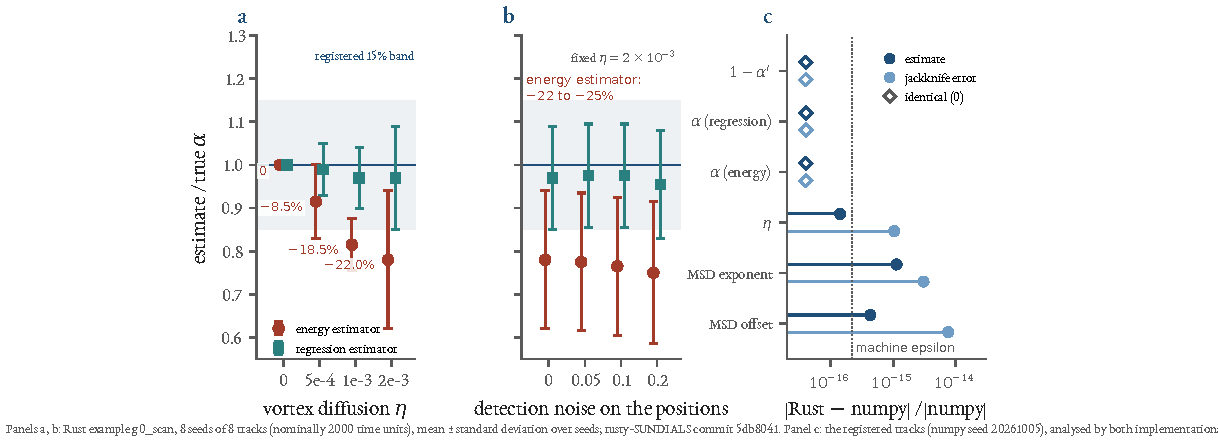
\includegraphics[width=\linewidth]{figures/ch10_estimator.pdf}
\caption[The energy estimator of the friction fails a known-answer test]{The energy estimator of the friction fails a known-answer test that it had passed once. \textbf{(a)}~Estimates divided by the true $\alpha=0.02$
as the diffusion $\eta$ of the model vortices grows, mean and standard deviation over \NxGateSeeds{} seeds of \NxGateTracks{} synthetic tracks
(Rust \texttt{g0\_scan}); the band is the registered 15~percent criterion. The identity of the theorem \texttt{energy\_dissipation} is exact
at $\eta=0$ and the energy estimator is exact there; the regression estimator stays near the truth. \textbf{(b)}~At $\eta=2\times10^{-3}$ the bias does not
depend on the detection noise added to the positions. \textbf{(c)}~The same eight tracks analysed by the numpy estimators and by the Rust estimators:
relative difference of every estimate.}\label{ch10:fig-estimator}
\end{figure}

Three things are visible in figure~\ref{ch10:fig-estimator}. First, in the noise-free model the energy estimator is exact (\NxGateEnergyZ{} against
$0.02$), as the theorem says it must be: the proved identity and the number agree where the hypothesis holds. Second, as soon as the vortices diffuse
the estimator is biased low, by \NxGateBiaseA, \NxGateBiaseB and \NxGateBiaseC~percent at the three diffusions tried, and the registered criterion
(within 15~percent) is met on only \NxQGatePassSeeds{} seeds in the programme's own count of this test; the gate had passed on, in the ledger's words,
``one lucky seed''. Third, the bias is not caused
by the detection noise: it is already there with none, and the energy estimator gives \NxGatenEnergyZ, \NxGatenEnergyA, \NxGatenEnergyB and \NxGatenEnergyC{} at
detection noise $0$, $0.05$, $0.1$ and $0.2$ per coordinate (panel~b). The regression estimator, which uses the same tracks, returns
\NxGateRegA, \NxGateRegB and \NxGateRegC{} at the same three diffusions and \NxGateOneminusapC{} for $1-\alpha'$ (truth $0.90$). Why the energy
estimator is biased we do not know. The programme's note suggests that the stochastic part of $H(t)$ is correlated with the cumulative regressor
$\int2\sum_i|\mathbf v_{s,i}|^2\mathrm dt$, which is computed from the same noisy path; that is a hypothesis, and is marked as one in the note.

Panel~(c) records what the second implementation did. The numpy estimators of the programme and the Rust estimators of \texttt{qf-pgpe} were run on
identical tracks and agree to \NxCrossMaxest{} in all six estimates and to \NxCrossMaxerr{} in their jackknife errors; on four real tracks the
software paper reports $2\times10^{-14}$ \cite{Callens2026sw}. On the registered tracks themselves (numpy seed 20261005), both implementations return $\alpha_{\rm energy}=\NxCrossEnergy$ --- the number with which the gate was recorded as
passed --- and $\alpha_{\rm regression}=\NxCrossReg$ with $1-\alpha'=\NxCrossOneminusap$. The agreement is the reason the Rust port could be trusted to expose a
defect, and the reason it could not have exposed this one by itself: two implementations of one estimator agree on its bias.

\subsection*{What it cost, and what it did not}

The programme's published friction values were computed with the energy estimator (CLAIM-098 of the ledger). The regression estimator is larger than the energy estimator by
$5$ to $21$~percent in the six measured arms, in exactly the direction of the bias, and the absolute values of $\alpha$ quoted in the first paper
\cite{Callens2026a} were therefore low by roughly \NxQBiasLo{} to \NxQBiasHi{}~percent. The coefficient of the temperature law
$\alpha/T$ rises from \NxQAlphatEnergy{} (energy) to \NxQAlphatReg{} (regression). The registered verdicts are comparisons between arms analysed with the same estimator, so none of them changes; both papers state the correction, the first in its results on the friction \cite{Callens2026a} and the second in its section on limits \cite{Callens2026b}.

\begin{keybox}[The rule]
A theorem is true of its hypotheses. Before an identity of the model is used as an estimator on data, test the estimator where the answer is known,
\emph{over many realisations}, and with the properties of the data (here: diffusion) switched on. This is the programme's rule LL-15 --- transfer a
result with its hypotheses, not just its conclusion --- applied to a theorem instead of to a measurement.
\end{keybox}

%=====================================================================================================================================
\section{What each check can and cannot see}\label{ch10:sec-checks}

The programme uses five kinds of check. Table~\ref{ch10:tab-checks} sets, for each, an instance in which it caught something and an instance, from
the same programme, in which it could not. None of the instances is hypothetical.

\begin{table}[tbp]\centering\footnotesize\renewcommand{\arraystretch}{1.15}
\begin{tabularx}{\linewidth}{@{}>{\raggedright\arraybackslash}p{0.14\linewidth}>{\raggedright\arraybackslash}X>{\raggedright\arraybackslash}X@{}}\toprule
check & caught, in this programme & could not see, in this programme\\\midrule
the Lean kernel and the axiom audit (Comparator: two kernels)
 & A count that had drifted: 76 theorems against 65 audit lines (RETRACTIONS.md, R3). A bug of the generator of the challenge files, which cut one
   statement at a \texttt{:=} inside a named argument, found while adding \brkident{SectorDuality} (CLAIM-052).
 & That the hypothesis of a true theorem fails in the data (section~\ref{ch10:sec-estimator}). That a true statement is empty: the dual-length bound is
   $x+1/x\ge2$ and ``could not have come out otherwise''. That a statement is the right physics: ``a Comparator pass says the solution proves the
   challenge's statement, not that the statement is the right physics'' (\brkident{docs/COMPARATOR\_SETUP.md}). That the hypotheses of a true theorem are met only by
   trivial cases: those of \texttt{KTFlow} (below, and \cref{ch06}).\\
a second implementation
 & A vortex centred on a grid node imprinted with modulus one instead of zero, in the first Rust version. A defect of the Adams order in the CVODE
   library, exposed by the first Hamiltonian system run through it. The estimator bias, once a seed sweep was cheap.
 & An error shared by both: numpy and Rust agreed to $2\times10^{-14}$ on four real tracks and both were biased. A platform effect that
   one platform hides: a $T=0$ control run that agrees to $10^{-13}$ on x86-64 differed by $8\times10^{-3}$ in position on an Apple-silicon runner.\\
a registered test
 & \NxVerdNotmet{} of \NxVerdCells{} criteria not met (figure~\ref{ch10:fig-verdicts}), each against a threshold written down beforehand.
 & A criterion that cannot fail for the reason intended: the residual criterion D-G2$''$ was ``mis-specified, since the vortex term is 500$\times$ the
   phonon term''. A battery of six criteria that all tested deterministic reproducibility in a chaotic model and none statistical reproducibility (LL-14).\\
the solver library's own tests
 & Nine tests of the Adams method of CVODE, written \emph{before} the fix of its defect (the method was implicit Euler); eight of them fail on the
   unfixed code (\brkident{crates/cvode/tests/adams\_order.rs}, \brkident{docs/CVODE\_ADAMS\_FIX.md}).
 & Which binary a script imports. The Python module installed in the shared environment of this book was built on 26~September, before the fix of 28~September:
   $y'=-y$ to $t=10$ at relative tolerance $10^{-10}$ cost \NxCvodeStaleNfe{} right-hand-side calls and returned an error of $\NxCvodeStaleErr$, against
   \NxCvodeFixedNfe{} calls and $\NxCvodeFixedErr$ for the build of commit 5db8041. The tests had run on the source. A convergence check in a chapter found the stale
   binary; no test did.\\
independent data
 & Two facts about a published reference run, found by trying to reproduce it: an $O(\Delta t)$ convention in its velocity ramp, and an initial field that
   is the Thomas--Fermi field after one imaginary-time step plus noise (the stopping rule is met at the first step).
 & Anything beyond the window reproduced: not $t>50$, not the Strouhal number, not single precision against discretisation; the model had to be recovered
   from the code, not from the paper's text.\\\bottomrule
\end{tabularx}
\caption{Five kinds of check, each with an instance of what it caught and of what it missed. Sources: RETRACTIONS.md, LEDGER.md (CLAIM-052, 079, 092, 098,
103, 106), LL.md (LL-14), the software paper \cite{Callens2026sw}, \texttt{docs/CVODE\_ADAMS\_FIX.md} of rusty-SUNDIALS, and the probe of appendix~\ref{appB}.}\label{ch10:tab-checks}
\end{table}

Two observations. The checks are not ordered by strength: each answers a different question --- is the statement what we think it is, does the code
compute what its author intended, does the binary that runs contain that code, was the verdict chosen before the data, does anyone else's data agree --- and
passing one is silent about the others. And a check is credited only when it has been \emph{run}. The programme's habit, visible in every row of the table, is to ask of a result
\emph{which} of these it has passed, and to write the answer down before anyone cites the result.

%=====================================================================================================================================
\section{The audit of the library}\label{ch10:sec-audit}

A sentence such as ``the library has \NxLibThm{} theorems, none uses \texttt{sorry}, all use only the three standard axioms'' is a claim about a
build, and it can be checked only by building. The programme's records show how easily it drifts. In September an external review of the v1.1.0
tag found that \brkident{DualLength.lean} declared 13 theorems while the reported count was 12; looking at all the files showed that \NxQRThreeListed{}
theorems existed where \NxQRThreeAudited{} carried a \texttt{\#print axioms} line, so \NxQRThreeMissed{} had never been audited and every published count
had conflated ``theorems'' with ``theorems carrying an audit line'' (RETRACTIONS.md, R3). The repair was a generator, \brkident{scripts/regen\_axiom\_audit.py},
which rewrites the audit block of every file and has a read-only \texttt{--check} mode.

For this book we audited the library again, differently. The driver (appendix~\ref{appB}; \brkident{book/facts/lean\_audit.py}) compiles each module,
in the order of its imports, against the pinned Mathlib (Lean 4.34.0-rc2, Mathlib tag v4.34.0-rc2), after appending to a scratch copy about twenty
lines of Lean --- new for this book, printed in appendix~\ref{appB} --- that walk the kernel environment of the module, ask \brkident{Lean.collectAxioms}
about \emph{every constant the file declares}, and print the union. It audits the environment, not the text: it needs no \texttt{\#print axioms} line
in the source. Like any auditor it has to be seen to catch something. Run on a file with planted defects it reports a \texttt{sorry}, the
same \texttt{sorry} inherited by a theorem whose own proof contains none, a \texttt{sorry} in a private theorem, an axiom declared by the module and
a use of \brkident{native\_decide}, and it reports the clean theorems as using at most \texttt{propext}, \brkident{Classical.choice} and \texttt{Quot.sound}
(\brkident{facts/audit\_controls/}). A grep for the word \texttt{sorry} in the compile log finds two of the three theorems that depend on a \texttt{sorry}; the third has no warning of its own.

\begin{figure}[!t]\centering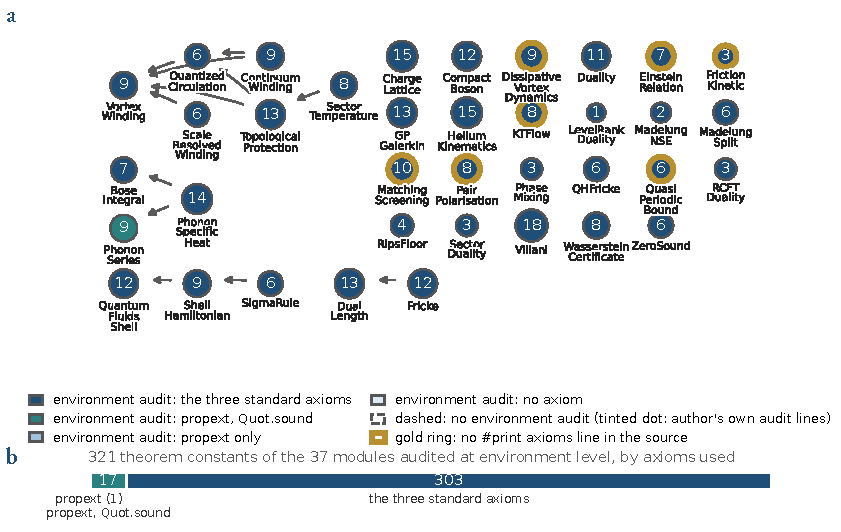
\includegraphics[width=\linewidth]{figures/ch10_library.pdf}
\caption[The library as audited for this book]{The library as audited for this book. \textbf{(a)}~The \NxLibModules{} modules, placed by the import relation (arrows point from a module to
the modules it imports), the size of a disc growing with the number of theorems of the module (printed inside); fill = the axiom footprint found by the environment audit, a dashed outline = no current
environment audit (\NxLibUnaudited{} when the figure was drawn), a gold ring = the module's source carries no \texttt{\#print axioms} line of its own (\NxLibNoprint{} modules). \textbf{(b)}~The axiom footprint of every theorem constant of
every module, from the environment audit.}\label{ch10:fig-library}
\end{figure}

\paragraph{What the audit found.} Five things are worth telling.

\emph{The first run of our own driver reported nine failures, and none was real.} It compiled each file separately, inside the Mathlib tree; nine
modules import a sibling (\texttt{import VortexWinding}) whose compiled file was not on that tree's search path, so Lean answered \texttt{unknown
module prefix}. The driver of this book builds in dependency order and puts the compiled siblings on the path.

\emph{Seven modules carry no \texttt{\#print axioms} line}, and their compile logs are therefore empty: \brkident{DissipativeVortexDynamics},
\brkident{EinsteinRelation}, \brkident{FrictionKinetic}, \texttt{KTFlow}, \brkident{MatchingScreening}, \brkident{PairPolarisation} and
\brkident{QuasiPeriodicBound}. An empty log of a module that compiles is not a timeout and not a failure; it is a module that was never asked. Asked (table~\ref{ch10:tab-seven}), each of the seven
compiles without error and depends on at most the three standard axioms; no \texttt{sorry} is reachable from any of their \NxAuditSevenThm{} theorems.
The staleness check introduced after R3 (\texttt{python3 scripts/regen\_axiom\_audit.py --check}, read-only) flags exactly these seven library modules (and four scratch files): the drift that R3
repaired reappeared within three weeks of its repair, for the same reason: the check exists, and no script, workflow or git hook of the repository calls it. The programme's gate
script \brkident{scripts/verify.sh} builds a single module (\brkident{QuantumFluidsShell}) and searches the log for \texttt{sorryAx}. The same seven
modules are also the ones that the Comparator list (\NxLibCmpModules{} modules, \NxLibCmpThm{} theorems, accepted by the Lean kernel and by
nanoda \cite{LeanComparator,Nanoda}) does not contain.

\InputIfFileExists{figures/ch10_audit_seven}{}{}

\emph{The generator that repaired the count has a blind spot of its own.} It recognises a theorem only at the start of a line, so
\brkident{crossover\_apply\_mem} and \brkident{crossover\_apply\_not\_mem} in \texttt{Villani.lean}, declared as \texttt{@[simp] theorem}, were never given an
audit line: the generator counts \NxLibGenThm{} theorems where the index of the library lists \NxLibThm{}. The generator of the Comparator's challenge files keeps the
theorems that carry an audit line, so it inherits the blind spot: the \NxLibCmpThm{} theorems that the Comparator accepted are the \NxLibCmpGen{} listed ones, out of
\NxLibCmpIdx{} in the thirty modules it covers (the two missing are the two above). \NxVillaniSimp

\emph{One module is outside the build.} \brkident{FrictionKinetic.lean} appears neither in \brkident{lakefile.lean} nor in the umbrella file
\brkident{QuantumFluids.lean}: \texttt{lake build} does not build it, and \texttt{import QuantumFluids} does not give its theorems.

\emph{The index of the library, from which this book's citations of theorems were first taken, was wrong about the names.} It said that every module lives in
the namespace \brkident{QuantumFluids.}\emph{Module}. For \NxLibOddNs{} of the \NxLibModules{} modules it does not: the seven newest modules sit in bare namespaces
(\brkident{KTFlow.kt\_trapped}), \texttt{Duality} sits in \brkident{Mathesis.Duality}, \brkident{QuantizedCirculation} in \brkident{QuantumFluids.Circulation},
and \brkident{QuantumFluidsShell}, \brkident{ShellHamiltonian} and \texttt{SigmaRule} in \brkident{QuantumFluids.ShellComplex}. The error was found only when the
catalogue of appendix~\ref{appA} was generated from the sources instead of typed, and the book's theorem-citation macro now looks the namespace up.
It is the same kind of error as the drifting count: a statement about the library that nobody had compared with the library.

\emph{The result.} \InputIfFileExists{figures/ch10_audit_result}{}{\textbf{[The environment audit had not finished when this text was generated; the sentence that reports it is written by \brkident{figures/ch10\_audit\_text.py} once the audit is complete.]}} \InputIfFileExists{figures/ch10_audit_book}{}{}

\paragraph{What the audit does not do.} It reads the environment that Lean's elaborator produced and trusts Lean's kernel; the second kernel is the
Comparator's business, and we did not re-run Comparator for this book (its results are those recorded in \brkident{docs/COMPARATOR\_SETUP.md}). It says
nothing about whether a statement is the right one; the statements are in appendix~\ref{appA} for a human to read, and a Comparator pass shows the same statement only because, in the words of the programme's own note,
``\,`same statement' is guaranteed by construction'' when the challenge file is generated from the solution. And it is only
as complete as the list of modules: the umbrella file and the lakefile are part of what has to be kept in step.

%=====================================================================================================================================
\section{What failed, plainly}\label{ch10:sec-failures}

The ledger of the programme (\texttt{LEDGER.md}) numbers its claims; in \NxLedgerDays{} days, from \NxLedgerFirst{} to \NxLedgerLast, it reached
claim \NxClaimsLast. Its entries carry statuses, and a good many of the statuses are the words \emph{retracted}, \emph{withdrawn}, \emph{refuted} or
\emph{void}. Only \NxClaimsChecked{} of the \NxClaims{} claims are in the format that the ledger's own checker (\brkident{scripts/check\_ledger.py})
reads; the rest are in a second, tabular format that it does not see --- a limitation of the machine check that the ledger itself records (CLAIM-066).
What follows is therefore a reading of the text, not a statistic.

\paragraph{A map of the verdicts.} Figure~\ref{ch10:fig-verdicts} draws every criterion that the ledger records one by one, for \NxVerdRows{} of the
programme's campaigns. There are \NxVerdCells{} of them: \NxVerdMet{} were met as registered, \NxVerdNotmet{} were not, \NxVerdMixed{} were mixed, partial
or inconclusive, one was voided afterwards and one was not run. The criteria are not independent and not equally important --- the kinetic benchmark
contributes $25$ cells, the finite-size ladder $7$ --- and the selection rule is the only one available to us: the campaigns whose per-criterion
outcomes the ledger gives. It shows how often a criterion written down before the data was not met, among those the ledger itemises: nearly as often as it was met.

\begin{figure}[tbp]\centering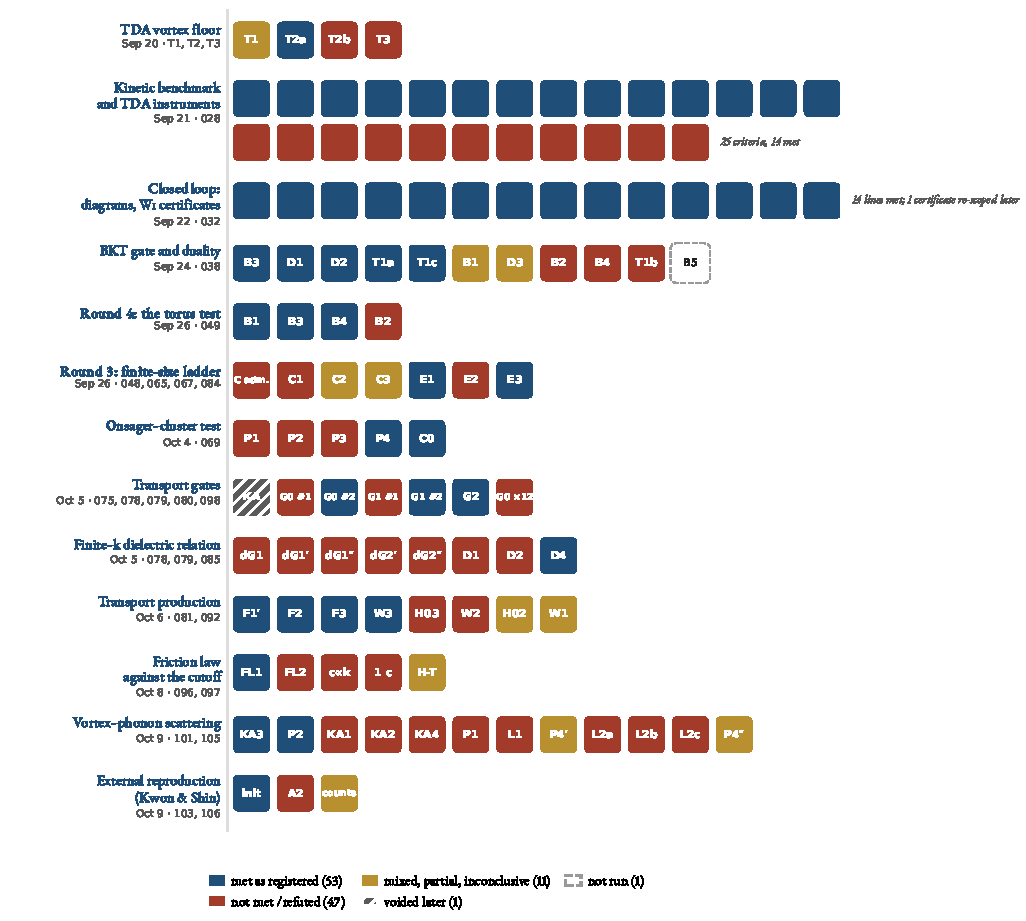
\includegraphics[width=\linewidth]{figures/ch10_verdicts.pdf}
\caption[Every criterion the ledger records, by campaign]{Every criterion that the ledger records one by one, by campaign (numbers are ledger claims; figure script \texttt{figures/ch10\_verdicts.py}
checks each row against \texttt{LEDGER.md}). Blue: met as registered; red: not met or refuted; gold: mixed, partial or inconclusive; hatched: voided
afterwards; dashed: not run. Unlabelled cells are criteria the ledger counts but does not name. Labels are those of the registration documents:
for instance P1--P3 are the registered predictions of the Onsager-cluster test (all three failed), G0/G1 the gates of the transport campaign (each
failed at its first attempt), D1/D2/D4 the criteria of the dielectric test, FL1/FL2 those of the friction-law test, L1/L2a--c those of the
vortex--phonon scattering test. The cell \emph{G0$\times12$} is the energy criterion of G0 re-run over many seeds (section~\ref{ch10:sec-estimator}).}\label{ch10:fig-verdicts}
\end{figure}

\paragraph{September: the literature check.} On 20~September the programme pre-registered a hypothesis, the \emph{dual scale} of a quantum fluid,
stated it in Lean, and refuted it for helium~II by measurement; the release of that day is tagged ``stated, proved, and refuted for He-II''. The same
day the literature check that the proposal itself had listed as blocking any claim of novelty was run, and it went against the programme on both
counts (RETRACTIONS.md). The second invariant of the complexified shell model was a rediscovery of structures in Vladimirova, Shavit and Falkovich's
\emph{Fibonacci turbulence} and in a second paper by overlapping authors on second-harmonic generation as a minimal model of turbulence
\cite{Vladimirova2021a,Vladimirova2021b}; on the dyadic lattice the family of conservation laws collapses to a single invariant, so the model has
\emph{less} structure than the published one. The dual length $\ell(k)=\varepsilon^2/(\hbar^2c^2k^3)$ was a repackaging of the static response, its
``bound'' was the inequality between the arithmetic and the geometric mean, it was weaker than the known linear bound of Onsager's inequality
\cite{WreszinskiDaSilva2005} outside a narrow window of wavenumbers, and its interior minimum was dimensionally forced; the ``refutation'' for helium
was structural, since any fluid with a roton violates it. The file states the outcome in one sentence: ``No novel scientific contribution survives
in the dual-scale programme.'' What survived were the Lean proofs, as correct mathematics of known results, the measurements, as correct measurements
of textbook physics, and a record of method. The same file lists a repository defect (a symlink to a local disk, committed by mistake, which broke every
clone) and the counting error of section~\ref{ch10:sec-audit}.

\paragraph{Failures of our own design.} Not every failure came from outside. Lessons LL-7 to LL-14 of the programme's \texttt{LL.md} record
what the first weeks cost. A table of literature constants entered the roton gap in kelvin and used it as millielectronvolts, overstating it by the
Boltzmann-constant factor, about $11.6$, and a conversion constant was off by exactly $2$; the synthetic tests had been generated with the same wrong
constants they checked, and both errors surfaced only against real, digitised data (LL-7). Values of the phonon--roton (Landau) parameters recalled from memory were attributed to two
papers that report no such values; they were within about $0.3$~percent of the true ones, which is why they survived (LL-10). An exponent fitted to the
supremum of the enstrophy was a property of the horizon chosen, because the supremum does not converge in the horizon for a conservative regulator,
and every quality signal --- $r^2>0.96$, disjoint confidence intervals, a timestep-refinement criterion passing at $0.00$~percent --- was good (LL-11).
The thermalisation time of the chaotic model has a coefficient of variation of $23$ to $49$~percent from one realisation to another at fixed parameters, and four rounds
of results had come from a single trajectory (LL-14). And a lesson that is not about physics: a destructive check of the Lean gate, which inserts a
\texttt{sorry} into a source file, was launched as one background command, outlived its foreground timeout, and the file still contained the
\texttt{sorry} when a commit was being prepared; ``the margin was one grep'' (LL-13).

\paragraph{October: the campaign.} The pre-registered campaigns of October produced most of the cells of figure~\ref{ch10:fig-verdicts}, and the
ledger reads like a lab book of an apparatus that did not work the first time. The friction known-answer gate of CLAIM-075 was recorded as passed on 5~October
and withdrawn the same day, when the first gates of the transport campaign were run, because the vortex imprint of the instrument added an amplitude tail four times the Bernoulli depletion and a phase step
along a whole line of the box, and the apparent friction at $T=0$ was as large as the thermal value being measured (CLAIM-078). The counterflow control
W2 was refuted, one run of four meeting the no-stall criterion (CLAIM-092). The friction law ``$\alpha\propto\rho_n$'' was found to be a degeneracy of
one cutoff, since $\rho_n\propto T$ there; across three cutoffs the coefficient is $0.31$, $0.23$ and $0.10$ and only $\alpha/T$ is constant
(CLAIM-096), and the paper that had published the first reading, together with a ``geometric core size of $1.4\,\xi$'' derived from it, had to be corrected in
version 2.2. The finite-k dielectric relation, tested mode by mode, held in one run of six; an earlier correlation of $0.996$ across runs had been carried by
box-scale pairs (CLAIM-085). The vortex--phonon scattering cross-section depended on the pair separation and on the box, and the registered conclusion is that an
isolated-vortex $\sigma_\parallel(k)$ ``is not defined by this observable at these geometries'' (CLAIM-105).

Two failures were failures of process rather than of physics. A verdict of ``saturation'' for the finite-size offset at $L=192$ (CLAIM-067,
admission $3$ of $6$) was recorded as unresolved, and a longer run (CLAIM-084, admission \NxQCFourAdm) showed that it had rested on states that had not
equilibrated; the finite-size trend of the whole ladder was then, in the ledger's words, under the same suspicion. And the first Python attempt
at those $L=192$ runs died silently after about \NxQCThreeHours{} hours, with nothing in its log; the cause could not be diagnosed, an out-of-memory
kill being ``the leading, unconfirmed hypothesis''. The runs were redone with a Rust port of the integrator, which itself stopped once without an error
and was resumed from a checkpoint.

A third process failure happened while this book was being written. The Python module \brkident{rusty\_sundials} installed in the shared environment had been built on
26~September (the stale module of the probe of appendix~\ref{appB}), two days before the Adams method of the solver library was repaired; in that build the method is implicit
Euler, and its work grows like $\mathrm{rtol}^{-1/2}$. The library's tests, written before the repair, fail on the old code, but they test the source, not the file that a script imports.
The defect was caught by a convergence check in one chapter. The probe of appendix~\ref{appB} (Adams on $y'=-y$ to $t=10$ at relative tolerance $10^{-10}$) separates the two
builds: \NxCvodeStaleNfe{} right-hand-side calls and an error of $\NxCvodeStaleErr$ before, \NxCvodeFixedNfe{} calls and $\NxCvodeFixedErr$ after. No computation of
this chapter used CVODE through that module; the lesson is the one of section~\ref{ch10:sec-estimator} applied to a binary: a check certifies the thing it was run on.

\begin{table}[tbp]\centering\small\renewcommand{\arraystretch}{1.12}
\begin{tabularx}{\linewidth}{@{}>{\raggedright\arraybackslash}p{0.11\linewidth}>{\raggedright\arraybackslash}p{0.27\linewidth}>{\raggedright\arraybackslash}X>{\raggedright\arraybackslash}X@{}}\toprule
when & what was withdrawn or corrected & what had failed & rule or repair\\\midrule
Aug 14--15 & exponent comparison, ordinal-censoring result (CLAIM-R1, R2, 012, 013) & horizon not converged; one trajectory of a chaotic system & LL-11, LL-14: converge in the horizon; measure the ensemble spread first\\
Aug & prediction exported to a sister project (CLAIM-017) & tested in their code before it was sent: exponent stable to four decimals over $8\times$ horizons & LL-15; retracted the same turn\\
Sep 20 & second invariant, dual length, $\sigma$-rule (CLAIM-023, 024, 025) & rediscovery; weaker than the known bound; dimensionally forced & RETRACTIONS.md; no novelty claimed\\
Sep 20 & TDA vortex floor (CLAIM-T1, T2, T3) & confounded by the segmentation threshold; split verdict; refuted & threshold-free line tracing; ``nothing from this run is citable''\\
Sep 21 & kinetic benchmark and TDA instruments (CLAIM-028) & \NxQKinNot{} of $25$ criteria not met; Lean formalisation of nonlinear Landau damping called ``out of reach'' six days after it had been posted \cite{Bedrossian2026} & literature gate before any claim of difficulty\\
Sep 22 & Wasserstein certificate, phase-space pair (CLAIM-032 erratum) & computed on $5$ points per side instead of the registered $30$; the same class of defect as a point list changed between workflow stages, found the same day & all pairs recomputed independently; erratum carried into the next paper\\
Oct 5 & friction known-answer gate (CLAIM-075 $\to$ 078) & imprint with an amplitude tail and a phase step & new imprint; gates G0--G2\\
Oct 8 & counterflow control W2 (CLAIM-092, 095) & $1$ of $4$ runs met the criterion; a template-filled paragraph contradicted the verdict & explanation withdrawn, observation kept; text corrected\\
Oct 8--9 & $\alpha\propto\rho_n$ and a core size of $1.4\,\xi$ (CLAIM-096, 099) & coefficient depends on the cutoff; $\rho_n\propto T$ degeneracy & paper corrected (v2.2); $\alpha/T$ reported\\
Oct 9 & energy estimator of $\alpha$ (CLAIM-098) & biased low by diffusion; gate passes on $2$ of $12$ seeds & regression estimator; gates run over seeds\\\bottomrule
\end{tabularx}
\caption{What was withdrawn or corrected, why, and the rule or repair that followed. Every row is an entry of \texttt{LEDGER.md}, \texttt{RETRACTIONS.md} or
\texttt{LL.md}.}\label{ch10:tab-failures}
\end{table}

\paragraph{Two statements that stayed true.} Not everything in the middle of a failed campaign fails. Two Lean statements of the transport campaign
illustrate what a proved statement does \emph{not} change.

\begin{leanbox}{QuasiPeriodicBound}
\begin{lstlisting}[style=lean]
noncomputable def qp (a ω φ : ι → ℝ) (t : ℝ) : ℝ := ∑ k, a k * Real.cos (ω k * t + φ k)

theorem not_qp_of_msd_large (a : ι → ℝ) {J : Type*} [Fintype J] [Nonempty J] (x : ℝ → ℝ) (ts τs : J → ℝ)
    (h : (2 * ∑ k, |a k|) ^ 2 < (∑ j, (x (ts j + τs j) - x (ts j)) ^ 2) / Fintype.card J) :
    ∀ ω φ : ι → ℝ, x ≠ qp a ω φ
\end{lstlisting}
\end{leanbox}

\noindent The first is the logic of a discriminant. A vortex pair whose motion is a regular island has quasi-periodic coordinates, finite sums of cosines;
the statement says that if the sampled mean-square increment of a signal exceeds $(2\sum_k|a_k|)^2$, the signal is not such a sum for \emph{any}
frequencies and phases with those amplitudes. The docstring is explicit that the decision rule is ``sound in one direction and silent in the other'': growth
refutes the island reading, a plateau proves nothing. On the data the registered criterion I2 was read as ``not an island'' --- the separations of the
stalled pairs carried a third of their variance in their three largest spectral lines, less than the registered half (CLAIM-086) --- and nothing about the
statement had to be revised.

\begin{leanbox}{FrictionKinetic}
\begin{lstlisting}[style=lean]
noncomputable def alpha (K : Finset ι) (w f : ι → ℝ) (ρs κ : ℝ) : ℝ := (∑ k ∈ K, w k * f k) / (ρs * κ)

noncomputable def rhoN (K : Finset ι) (w : ι → ℝ) : ℝ := ∑ k ∈ K, w k

theorem coeff_eq_weighted_mean (K : Finset ι) (w f : ι → ℝ) (ρ ρs κ : ℝ) (hρn : rhoN K w ≠ 0) (hρ : ρ ≠ 0) :
    alpha K w f ρs κ / (rhoN K w / ρ) = ρ / (ρs * κ) * ((∑ k ∈ K, w k * f k) / ∑ k ∈ K, w k)
\end{lstlisting}
\end{leanbox}

\noindent The second is an identity of a kinetic model of the friction: if the drag and the normal density are sums over the same bath modes $k\in K$ with the
same nonnegative weight $w_k$, the drag carrying one more factor $f_k$ (group velocity times transport cross-section), then the ratio $\alpha/(\rho_n/\rho)$
is a constant times the $w$-weighted mean of $f$ over the modes (the proof is algebra: abridged here). What the statement says about the world is only
that this coefficient is a property of the \emph{bath}: it can depend on the modes retained. It does not say that it is independent of the cutoff, and when
the registered expectation that it nearly is (spread below $0.2$) failed --- the coefficient was $0.31$, $0.23$ and $0.10$ at the three cutoffs --- the
identity was not affected. What was withdrawn was a reading of the number measured at one cutoff, a ``geometric core size of $1.4\,\xi$''. The theorem
is a statement about the model, the $1.4\,\xi$ was a statement about the world, and only the first had been proved.

\paragraph{A statement that was true and nearly empty.} A third statement was true, and its trouble was of the opposite kind: in the estimator story a hypothesis failed in the data, here a hypothesis
can hardly be met by anything. It was found while \cref{ch06} was being prepared. Three theorems of \texttt{KTFlow} (\Lthm{KTFlow}{kt_invariant}, \Lthm{KTFlow}{kt_trapped} and
\Lthm{KTFlow}{kt_fugacity_bounded}) are about a solution $(u,y)$ of the Kosterlitz flow, and the file asks for the two flow equations and for $u>0$ \emph{at every real
scale} $l$, negative ones included (the hypotheses \texttt{hu}, \texttt{hy} and \texttt{hpos} are quantified over all $l\in\mathbb R$), whereas a renormalisation
trajectory is a solution for $l\ge0$ only. \Cref{ch06} proves, in a new module of the book, that on the superfluid side these hypotheses leave almost nothing: if
$u(0)<\pi/2$ then $y(0)=0$. (If $y(0)\neq0$, the invariant forces $y(l)^2\ge y(0)^2$ for $l\le0$, so going backward $u$ would fall at least linearly and be negative
before $l=-u(0)/c$, with $c=4\pi^3y(0)^2$, which the hypothesis $u>0$ forbids.) From $y(0)=0$ the uniqueness of the solution of the linear equation for $y$ gives
$y\equiv0$ and $u$ constant --- a standard step, not formalised --- so only fixed points of the flow meet the hypotheses there. The three theorems are true, and the
kernel certified exactly what had been written; what had been written asked too much of a solution to be applied to one that matters. The library file is unchanged; \cref{ch06} restates the theorems under hypotheses on
$l\ge0$ only, and adds the converse.

\paragraph{A name that was copied, not checked.} The 2021 paper of Godfrin and his co-authors \cite{Godfrin2021} has seven authors. While this book was written its
record at the publisher (Crossref) was compared with the programme's own notes, and two of them gave the list wrongly: the literature ledger wrote the second
author's initial as M instead of K, and a design note, like the docstring of the library module \brkident{PhononSeries}, named an eighth author who is not on the paper.
No test could catch a name, and none did; the slips were found by looking the record up. They were corrected on 10~October 2026 (in the library the change is a
comment, so no theorem is touched); the copy of that module that is generated for the Comparator repeats the old docstring until its generator is run again.
It is the lesson of the other paragraphs at the smallest scale: a copy of a copy is not a source.

\paragraph{What the failures have in common.} The following is our reading, not a measurement. Most of the entries of table~\ref{ch10:tab-failures}
fall into three kinds: a result used outside the hypotheses on which it depended (the estimator; the prediction exported to a sister project; the
friction law outside one cutoff); one realisation mistaken for an ensemble (the single trajectories of August, the single seed of G0, a single seed
per energy at $L=192$); and a gate or a criterion that could not fail for the reason intended (the battery of LL-14, the imprint that made the
known-answer gate pass, the residual criterion D-G2$''$). They are the same three mistakes at three scales, and each has a cheap check, which is
what the rules of the programme are: write down the hypotheses and check them in the target (LL-15), measure the spread before fitting (LL-14),
and run the gate where the answer is known with the property switched on (section~\ref{ch10:sec-estimator}). They are also the reason that pre-registration
\cite{Nosek2018} is only half a method: a registered criterion makes the verdict impossible to bend, and does nothing about whether the criterion could
have failed for the right reason.

%=====================================================================================================================================
\section{Speed is a claim too}\label{ch10:sec-speed}

The solver of this book is offered as a tool, and a tool has a speed; claims of speed are checked less often than claims of physics. The benchmark of
the software paper \cite{Callens2026sw} times one step of the projected Gross--Pitaevskii integrator on an $N\times N$ grid ($L=N/2$, $g=1$,
$\Delta t=0.01$), identical in every engine; the final states agree in a checksum (to \NxBenchJaxchk{} for JAX against Rust), so the timings are for the same computation.

\begin{figure}[!t]\centering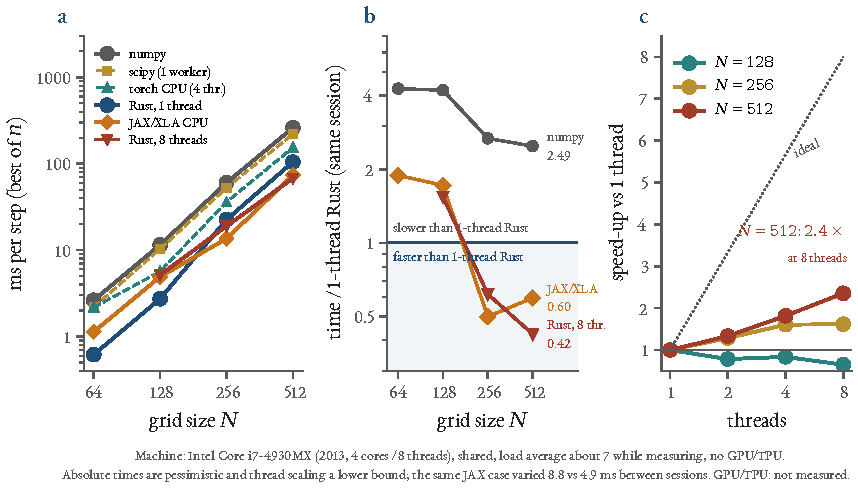
\includegraphics[width=\linewidth]{figures/ch10_bench.pdf}
\caption[Time per step of the projected Gross--Pitaevskii integrator in several engines]{Time per step of the projected Gross--Pitaevskii integrator in several engines (best of $n$ repetitions). \textbf{(a)}~Absolute time against grid size
$N$. \textbf{(b)}~Time relative to the one-thread Rust step measured in the same session, so that load common to both cancels in part; values below one
are faster than serial Rust. \textbf{(c)}~Speed-up of the threaded Rust step against its own one-thread time. All measurements were taken on one shared
machine (Intel Core i7-4930MX, 2013, 4 cores and 8 threads, load average $\approx7$, no GPU); the same JAX case gave $8.8$~ms in one session and
$4.9$~ms in another. Data: \texttt{data/generated/pgpe/bench/}.}\label{ch10:fig-bench}
\end{figure}

On one thread the Rust engine takes \NxBenchRustA, \NxBenchRustB, \NxBenchRustC{} and \NxBenchRustD~ms per step at $N=64$, $128$, $256$, $512$, against
\NxBenchNumpyA, \NxBenchNumpyB, \NxBenchNumpyC{} and \NxBenchNumpyD~ms for numpy: \NxBenchSpnpA, \NxBenchSpnpB, \NxBenchSpnpC{} and \NxBenchSpnpD{} times faster,
the advantage shrinking with $N$. A JAX/XLA version on the CPU is slower than serial Rust at $N=64$ and $128$ and faster at $N\ge256$; pinned to one core
the order reverses, so the XLA lead at large $N$ is threading and not a better algorithm. Threading the Rust step helps at $N\ge256$
(\NxBenchThrBig$\times$ at $N=512$ on eight threads, \NxBenchThrMid$\times$ at $N=256$) and \emph{hurts} at $N=128$:
\NxBenchSmallEight~ms on eight threads against \NxBenchSmallOne~ms on one, so for small grids the threading must stay off.

What is not claimed matters as much. There is no comparison with FFTW-based C codes, with GPU codes or with any other published solver, and no
measurement on a GPU or a TPU; the machine was shared, so absolute times are pessimistic and the scaling is a lower bound; the statistic is the best
of a few repetitions, taken in the same way for every engine, in two sessions that differ by up to a factor of two for the same case. ``Fast'' in this
book means ``faster than numpy on this machine, for this problem, on one thread''. It does not mean ``the best solver''.

%=====================================================================================================================================
\section{What a reader can reuse}\label{ch10:sec-legacy}

\paragraph{The library.} The Lean library \cite{Callens2026lib} is \NxLibModules{} modules and \NxLibThm{} theorems and lemmas, with \NxLibDef{} definitions,
structures and abbreviations (catalogue in appendix~\ref{appA}). It is pinned to Lean 4.34.0-rc2 and to the Mathlib tag of the same name, and is licensed
MIT or Apache-2.0. A reader who wants a result, rather than a method, should look first at the modules whose subject is mathematics with a physical
reading: \texttt{BoseIntegral}, \texttt{PhononSeries} and \brkident{PhononSpecificHeat} (the coefficients of the phonon specific-heat series),
\texttt{ZeroSound} (when an undamped zero-sound root exists), \brkident{VortexWinding} and \brkident{QuantizedCirculation} (that the way simulation codes find
vortices measures an integer), \texttt{KTFlow} (the Kosterlitz renormalisation flow). Every module is a top-level module of its own: the umbrella file
\brkident{QuantumFluids} imports all but one.

\begin{godfrinbox}{the series of Eq.\,(22), and a remark of its authors}
In the paper on the dispersion relation of the Landau excitations of superfluid $^4$He, measured by inelastic neutron scattering on IN5 at the ILL,
Godfrin and co-authors give in Eq.\,(22) the phonon specific heat $C_V=AT^3+CT^5+DT^6+ET^7+KT^8+LT^9$ for a dispersion
$\varepsilon=\hbar ck(1+\alpha_2k^2+\dots+\alpha_6k^6)$ with $\alpha_1=0$, and remark that earlier published versions of this series contain
errors \cite{Godfrin2021}. The library has derived the six coefficients independently (with sympy) and proved them in Lean
(\texttt{BoseIntegral}, \texttt{PhononSeries}, \brkident{PhononSpecificHeat}): a confirmation of the paper's Eq.\,(22), not a finding. What is proved is
the mathematical statement, a series coefficient; it is not a statement about the experiment.
\end{godfrinbox}

A series of six terms, each a polynomial in the coefficients of the dispersion relation, is algebra that a machine can check at small cost; but the
same remark applies to it as to everything above: the kernel certifies the algebra, and the physics of the dispersion relation is in the measurement.

\paragraph{The solver.} The engine \texttt{qf-pgpe} of rusty-SUNDIALS (release v11.6.0; software paper \cite{Callens2026sw}) is a pure-Rust
projected Gross--Pitaevskii integrator with a Python extension, \texttt{qf\_pgpe}, whose \texttt{Pgpe}, \texttt{imprint\_v2}, \texttt{detect} and
\brkident{analyse\_tracks} are drop-in replacements for the numpy versions of the programme; CVODE \cite{Hindmarsh2005} is available through
\brkident{rusty\_sundials} (take the build of commit 5db8041 or later, and check it with the probe of appendix~\ref{appB}). What is reusable beyond the code is the
verification harness: the cross-language comparison on identical inputs, the CVODE reference, run with the repaired Adams method, that confirms the fourth order
of the step, and a reproduction test of the Kwon and Shin run \cite{KwonShin2026data} on its real download,
which runs weekly and on demand outside the required checks (\cref{ch09}).

\paragraph{The discipline.} It is the part of the programme that held up under its own failures, and it is small enough to list.
\begin{keybox}[A checklist, from the programme's practice and from the making of this book]
\begin{enumerate}[nosep,label=\arabic*.]
\item Register the criteria, the decision rule and the kill rule \emph{before} the data exist, in a file under version control \cite{Nosek2018}.
\item Give every instrument a known-answer test, run it over many realisations and with the property of the data that will matter switched on.
\item Have a second implementation, or a second source of data, for every number that will be quoted.
\item Write down the hypotheses of a result before exporting it, and test each in the target (LL-15).
\item Give every constant that stands for a measurement its source, table and uncertainty in a comment beside it (LL-10).
\item Read the literature for the claim of novelty \emph{and} for the claim of difficulty before either is made.
\item Keep a ledger with statuses that include \emph{refuted} and \emph{withdrawn}, and correct a published number in the next version of the paper that
 carries it.
\item Look a citation up in the publisher's record before it is printed; a copy of a copy is not a source.
\item Make the record reproducible from files: a script for every figure, a source for every number (appendix~\ref{appB} lists the scripts of this book) \cite{Peng2011}.
\end{enumerate}
\end{keybox}

%=====================================================================================================================================
\section{What is still open}\label{ch10:sec-open}

The following items are open in the programme's own records; none is a promise.

\begin{itemize}[nosep]
\item \emph{The cause of the energy-estimator bias} is not established; the regression estimator is the unbiased one, and a mechanism has to be
  derived or ruled out (exercise~1).
\item \emph{The temperature law of the friction}, $\alpha/T\approx\NxQAlphatEnergy$ (energy) or $\NxQAlphatReg$ (regression), independent of the cutoff
  over the three cutoffs tried, has no theory; the kinetic reading that was meant to explain it was withdrawn, and the single-pinned-vortex
  follow-up that would define an isolated-vortex cross-section was not started.
\item \emph{The finite-size offset} of the Josephson relation is positive at every size when the states are equilibrated, but the $L=128$ states are
  now under the suspicion that the $L=192$ ones were; the trend with $L$ is not established.
\item \emph{Counterflow}: the stall observed in the closed box is a bath-driven stall with a $1/f^{0.5}$ spectrum; the explanation that predicted its box-size
  dependence was withdrawn when the control W2 was refuted.
\item \emph{External reproduction}: one published run has been reproduced, to $t=50$; the plan's own criterion ($10^{-5}$ to $t=10$) was not met
  ($\NxQKsATwo$); the vortex counts agree at \NxQKsCounts{} times; nothing is shown for $t>50$ or for the Strouhal number.
\item \emph{Speed}: no idle-machine repetition, no GPU or TPU measurement; JAX is the proposed path to both.
\item \emph{Data}: no open numerical table of the Landau parameters of two-dimensional $^3$He has been found, in two independent searches; \cref{ch08}
  proves the existence criterion for zero sound, and a comparison with the film measurements of \cite{Godfrin2012} needs those parameters.
\item \emph{Housekeeping}: \brkident{FrictionKinetic} is outside the lakefile; seven modules have no audit line and are outside the Comparator list; the
  ledger has two formats and its checker reads one; the theorems of \texttt{KTFlow} should be restated for $l\ge0$ as in the book's module (\cref{ch06}).
\end{itemize}

A last remark on what the book is for. The experiments that frame it --- inelastic neutron scattering on two-dimensional liquid $^3$He \cite{Godfrin2012}
and on superfluid $^4$He \cite{Godfrin2021} --- end in numbers: a dispersion with a roton-like minimum, a specific-heat series. The programme described here
has no measurement of helium of its own to offer. What it can offer is a way of making calculations \emph{around} such numbers answerable: a theorem that can
be recompiled, a figure that can be regenerated, a failure that can be read in a ledger. That is the only sense in which a book of this kind can be a
tribute without claiming a partnership with the people it admires: it tries to be useful to whoever has next to check a series, rebuild a figure, or decide
whether a simulated vortex agrees with a measured one.

%=====================================================================================================================================
\begin{honestbox}
\textbf{Proved (Lean).} The theorem \Lthm{DissipativeVortexDynamics}{energy_dissipation} and its companions are theorems of the point-vortex model;
they are not statements about a simulated field or about a vortex in helium. For the modules it covers, the environment audit shows that every
theorem constant depends on at most \texttt{propext}, \brkident{Classical.choice} and \texttt{Quot.sound}; appendix~\ref{appA} marks, module by module,
whether that covers the module. It does not show that a statement is the right one. \textbf{Simulated.} The estimator bias, the numpy--Rust agreement
and the benchmark are results of runs, on synthetic tracks and on one shared machine; they say nothing about helium. \textbf{Not established.} Why the
energy estimator is biased; whether each Lean statement is the right physics (a human audit, not a kernel check); anything about a GPU.
\textbf{Analogy only.} Reading the failures of the programme as three recurring mistakes is our summary of the ledger, not a measurement of how often
they occur. \textbf{Failed or withdrawn} (sections~\ref{ch10:sec-estimator} and~\ref{ch10:sec-failures}): the energy-estimator gate that had passed
once; the friction known-answer gate of CLAIM-075; the counterflow control W2; the reading $\alpha\propto\rho_n$ with a core size of $1.4\,\xi$; the novelty
of the dual-scale programme; \NxVerdNotmet{} of the \NxVerdCells{} criteria drawn in figure~\ref{ch10:fig-verdicts}. Nothing in this chapter says that
Henri Godfrin, his collaborators or any laboratory has used, reviewed or endorsed this library.
\end{honestbox}

%=====================================================================================================================================
\section*{Exercises}

\paragraph{Exercise 1.} In the plane the vortex energy is $H=-\sum_{i<j}q_iq_j\ln r_{ij}^2$. Apply Itô's formula to $H(\mathbf r(t))$ for the
stochastic model (\ref{ch10:eq-model}) and show that the diffusion changes the mean drift of $H$ only through $\eta\,\Delta H$, which vanishes away from
coincidences because the logarithm is harmonic. (On the torus the neutralising background adds a constant.) The mean drift of $H$ is therefore
\emph{not} where the bias of the energy estimator comes from. Where could it come from? \emph{Hint:} the estimator is a regression of $H(t)$ on a running
integral of $S=\sum_i|\mathbf v_{s,i}|^2$; compute the covariance of the noise part of $H$ with that integral.

\paragraph{Exercise 2.} Write a Lean command that, for the module it is appended to, prints the number of theorem constants whose axiom set is strictly
smaller than $\{$\texttt{propext}, \brkident{Classical.choice}, \texttt{Quot.sound}$\}$, and run it on \texttt{BoseIntegral} and on \texttt{PhononSeries}. Which of
the two do you expect to give a positive count, and why? Compare with the footprints listed in appendix~\ref{appA}. \emph{Hint:} start from the program in
appendix~\ref{appB}; \brkident{ConstantInfo.isTheorem}, \brkident{Lean.collectAxioms} and \brkident{Name.isInternal} are all you need. One of the two files proves identities in
an arbitrary commutative ring by \texttt{linear\_combination}, the other is real analysis.

\paragraph{Exercise 3.} In figure~\ref{ch10:fig-bench}c the eight-thread step at $N=512$ is $\NxBenchThrBig\times$ faster than the serial one.
Use Amdahl's law to find the serial fraction $s$ that this implies (the speed-up on $p$ threads is $[s+(1-s)/p]^{-1}$) and predict the speed-up at $p=4$;
compare with the measured value in \brkident{ch10\_bench\_numbers.json}. At $N=128$ the same law cannot produce a slowdown: add a per-thread
synchronisation cost to the model and estimate the size of the step below which threading cannot pay. Which of your numbers would change on an idle
machine? \emph{Hint:} with $s=0.34$ the model gives $2.4$ at $p=8$; fit $t(p)=t_1[s+(1-s)/p]+c\,p$ to the three sizes of the figure.

%=====================================================================================================================================
\section*{Notes and further reading}

The three instruments of the book are described in their own papers: the Lean library \cite{Callens2026lib} (built on Lean~4 \cite{deMoura2021} and
Mathlib \cite{Mathlib2020}), the solver and its verification \cite{Callens2026sw}, and the physical programme \cite{Callens2026a,Callens2026b}. The
Comparator \cite{LeanComparator} judges that a Lean solution proves the statement of a challenge file under a list of permitted axioms, and can pass
the exported proof to a second kernel such as nanoda \cite{Nanoda}. Pre-registration as a general practice is discussed by Nosek and
co-authors \cite{Nosek2018}, and the case for publishing the code and the data from which a number was computed by Peng \cite{Peng2011}; both are
general discussions, and the checklist of section~\ref{ch10:sec-legacy} adapts them to this programme. The projected Gross--Pitaevskii method
that the solver implements is reviewed by Blakie and co-authors \cite{Blakie2008}. So far, the only experiment of this book that the programme has reproduced
independently is that of Kwon and Shin \cite{KwonShin2026prr}.
}
\appendix
\IfCh{appA}{\chapter{The Lean Library: a Complete Catalogue}\label{appA}
\providecommand{\citedmark}[1]{\textcolor{qfgold}{$\star$}{\fontsize{6}{6}\selectfont\,#1}}
\lstdefinestyle{leancat}{style=lean,basicstyle=\ttfamily\fontsize{8.4}{9.9}\selectfont,columns=fixed,xleftmargin=0.9em,xrightmargin=0pt,aboveskip=1.6pt,belowskip=2.8pt,breakindent=1.0em,escapeinside={;}{;}}
\noindent This appendix lists the whole of the Lean~4 library \lean{QuantumFluids} that the book is about: 37 modules, 310 theorems and lemmas, and 103 definitions, structures and abbreviations. It is \emph{generated} from the sources in \texttt{lean\_src/} by \texttt{book/facts/make\_appA.py} (see appendix~\ref{appB}); nothing in it is typed by hand except these paragraphs. Every statement is copied verbatim, line breaks included, up to the \texttt{:=} that starts its proof or definition body; the proofs are not reproduced.
\paragraph{How to read an entry.} Each module is headed by one line of its own docstring, by the namespace in which its declarations live (for 13 of the 37 modules this is \emph{not} \texttt{QuantumFluids.}\emph{Module}; see table~\ref{appA:tab-ns}), by the numbers of theorems and of definitions, and by its audit status. A gold $\star$ in the margin followed by chapter numbers marks a declaration that those chapters cite (through \texttt{\textbackslash Lthm} or by copying its statement). The catalogue is a statement of \emph{what is proved}, not of what is measured: to read a statement as physics, go to the chapter that cites it.
\paragraph{What the audit status means.} \emph{The audit is of the kernel environment, not of the source text.} For each module the book's audit driver (\texttt{book/facts/lean\_audit.py}, appendix~\ref{appB}) compiles the module in dependency order against the pinned Mathlib and asks Lean, for \emph{every constant the file declares}, which axioms it depends on (\texttt{Lean.collectAxioms}). The status line reports the number of theorem constants found, whether \texttt{sorryAx} is reachable, the number of axioms the module declares itself, and the union of the axioms used. The three standard axioms are abbreviated $p$ = \texttt{propext}, $c$ = \texttt{Classical.choice}, $q$ = \texttt{Quot.sound}. At the time this appendix was generated, 37 of 37 modules had such an environment audit on file; 0 more carry only the first-pass compile log (author-written \texttt{\#print axioms} lines, marked $^\dagger$ in the table); for the remaining 0 the status reads ``not re-checked''. Compiling a module with exit code~0 is not the same as auditing it: 7 modules (\texttt{DissipativeVortexDynamics}, \texttt{EinsteinRelation}, \texttt{FrictionKinetic}, \texttt{KTFlow}, \texttt{MatchingScreening}, \texttt{PairPolarisation}, \texttt{QuasiPeriodicBound}) carry no \texttt{\#print axioms} line in their sources, so a compile log of theirs is empty; the environment audit is what supplies their footprint (chapter~\ref{ch10}).
\begin{table}[p]\centering\footnotesize\setlength{\tabcolsep}{3.2pt}
\caption{The 37 modules of the library at a glance. \emph{thm}: theorems and lemmas; \emph{def}: definitions, structures, abbreviations; \emph{audit}: axiom footprint ($p$, $c$, $q$ as in the text; \texttt{n/c}: not re-checked; \texttt{stale}: the file changed after it was audited; \texttt{!}: a non-standard axiom or \texttt{sorryAx}); \emph{cited by}: chapters that cite a declaration of the module.}\label{appA:tab-modules}
\begin{tabular}{@{}lrrll@{}}\toprule module & thm & def & audit & cited by \\\midrule
\hyperref[appA:BoseIntegral]{BoseIntegral} & 7 & 2 & p c q & 1, 4 \\
\hyperref[appA:ChargeLattice]{ChargeLattice} & 15 & 4 & p c q & -- \\
\hyperref[appA:CompactBoson]{CompactBoson} & 12 & 3 & p c q & -- \\
\hyperref[appA:ContinuumWinding]{ContinuumWinding} & 9 & 1 & p c q & 3 \\
\hyperref[appA:DissipativeVortexDynamics]{DissipativeVortexDynamics} & 9 & 1 & p c q & 7, 10 \\
\hyperref[appA:DualLength]{DualLength} & 13 & 3 & p c q & -- \\
\hyperref[appA:Duality]{Duality} & 11 & 0 & p c q & -- \\
\hyperref[appA:EinsteinRelation]{EinsteinRelation} & 7 & 3 & p c q & 7 \\
\hyperref[appA:Fricke]{Fricke} & 12 & 3 & p c q & -- \\
\hyperref[appA:FrictionKinetic]{FrictionKinetic} & 3 & 2 & p c q & 7, 10 \\
\hyperref[appA:GPGalerkin]{GPGalerkin} & 13 & 7 & p c q & 2 \\
\hyperref[appA:HeliumKinematics]{HeliumKinematics} & 15 & 4 & p c q & 1, 4, 5, 9 \\
\hyperref[appA:KTFlow]{KTFlow} & 8 & 2 & p c q & 6, 10 \\
\hyperref[appA:LevelRankDuality]{LevelRankDuality} & 1 & 2 & p c q & -- \\
\hyperref[appA:MadelungNSE]{MadelungNSE} & 2 & 3 & p c q & 3 \\
\hyperref[appA:MadelungSplit]{MadelungSplit} & 6 & 1 & p c q & 3, 9 \\
\hyperref[appA:MatchingScreening]{MatchingScreening} & 10 & 3 & p c q & 6 \\
\hyperref[appA:PairPolarisation]{PairPolarisation} & 8 & 2 & p c q & 6 \\
\hyperref[appA:PhaseMixing]{PhaseMixing} & 3 & 0 & p c q & 8 \\
\hyperref[appA:PhononSeries]{PhononSeries} & 9 & 10 & p q & 2, 4 \\
\hyperref[appA:PhononSpecificHeat]{PhononSpecificHeat} & 14 & 1 & p c q & 1, 4 \\
\hyperref[appA:QHFricke]{QHFricke} & 6 & 3 & p c q & -- \\
\hyperref[appA:QuantizedCirculation]{QuantizedCirculation} & 6 & 3 & p c q & 1, 3 \\
\hyperref[appA:QuantumFluidsShell]{QuantumFluidsShell} & 12 & 3 & p c q & -- \\
\hyperref[appA:QuasiPeriodicBound]{QuasiPeriodicBound} & 6 & 1 & p c q & 7, 10 \\
\hyperref[appA:RCFTDuality]{RCFTDuality} & 3 & 1 & p c q & -- \\
\hyperref[appA:RipsFloor]{RipsFloor} & 4 & 2 & p c q & -- \\
\hyperref[appA:ScaleResolvedWinding]{ScaleResolvedWinding} & 6 & 4 & p c q & 3 \\
\hyperref[appA:SectorDuality]{SectorDuality} & 3 & 0 & p c q & -- \\
\hyperref[appA:SectorTemperature]{SectorTemperature} & 8 & 5 & p c q & -- \\
\hyperref[appA:ShellHamiltonian]{ShellHamiltonian} & 9 & 2 & p c q & -- \\
\hyperref[appA:SigmaRule]{SigmaRule} & 6 & 3 & p c q & -- \\
\hyperref[appA:TopologicalProtection]{TopologicalProtection} & 13 & 2 & p c q & -- \\
\hyperref[appA:Villani]{Villani} & 18 & 8 & p c q & -- \\
\hyperref[appA:VortexWinding]{VortexWinding} & 9 & 2 & p c q & 1, 3, 9 \\
\hyperref[appA:WassersteinCertificate]{WassersteinCertificate} & 8 & 6 & p c q & -- \\
\hyperref[appA:ZeroSound]{ZeroSound} & 6 & 1 & p c q & 1, 8 \\
\bottomrule\end{tabular}\end{table}
\begin{table}[t]\centering\footnotesize\setlength{\tabcolsep}{3.2pt}
\caption{Modules whose declarations do \emph{not} live in \texttt{QuantumFluids.}\emph{Module}. The fully qualified name of a theorem is the namespace below, a dot, and the name printed in the catalogue.}\label{appA:tab-ns}
\begin{tabular}{@{}ll@{}}\toprule module & namespace in the source \\\midrule
DissipativeVortexDynamics & \texttt{DissipativeVortexDynamics} \\
Duality & \texttt{Mathesis.\allowbreak{}Duality} \\
EinsteinRelation & \texttt{EinsteinRelation} \\
FrictionKinetic & \texttt{FrictionKinetic} \\
KTFlow & \texttt{KTFlow} \\
MadelungSplit & \texttt{QuantumFluids.\allowbreak{}Madelung} \\
MatchingScreening & \texttt{MatchingScreening} \\
PairPolarisation & \texttt{PairPolarisation} \\
QuantizedCirculation & \texttt{QuantumFluids.\allowbreak{}Circulation} \\
QuantumFluidsShell & \texttt{QuantumFluids.\allowbreak{}ShellComplex} \\
QuasiPeriodicBound & \texttt{QuasiPeriodicBound} \\
ShellHamiltonian & \texttt{QuantumFluids.\allowbreak{}ShellComplex} \\
SigmaRule & \texttt{QuantumFluids.\allowbreak{}ShellComplex} \\
\bottomrule\end{tabular}\end{table}
\section{The catalogue, module by module}
\subsection{BoseIntegral}\label{appA:BoseIntegral}
{\footnotesize\raggedright\texttt{The Bose integral behind the phonon specific heat of superfluid helium.\allowbreak{}}\par}
{\footnotesize\raggedright\emph{Namespace} \texttt{QuantumFluids.\allowbreak{}BoseIntegral} $\cdot$ 7 theorems, 2 definitions $\cdot$ \emph{audit}: 7 theorem constants audited (+1 generated by Lean), 0 sorry, 0 user axioms; axioms used: Classical.choice, Quot.sound, propext.\par}
\vspace{1pt}
\begin{lstlisting}[style=leancat]
;\llap{\citedmark{4}\,};noncomputable def bose (t : ℝ) : ℂ
\end{lstlisting}

\begin{lstlisting}[style=leancat]
;\llap{\citedmark{4}\,};theorem hasSum_bose {t : ℝ} (ht : t ∈ Ioi (0 : ℝ)) :
    HasSum (fun n : ℕ => (1 : ℂ) * rexp (-((n : ℝ) + 1) * t)) (bose t)
\end{lstlisting}

\begin{lstlisting}[style=leancat]
theorem hasSum_mellin_bose {s : ℂ} (hs : 1 < s.re) :
    HasSum (fun n : ℕ => Complex.Gamma s * 1 / (((n : ℝ) + 1 : ℝ) : ℂ) ^ s) (mellin bose s)
\end{lstlisting}

\begin{lstlisting}[style=leancat]
;\llap{\citedmark{1,4}\,};theorem mellin_bose_four : mellin bose 4 = (π : ℂ) ^ 4 / 15
\end{lstlisting}

\begin{lstlisting}[style=leancat]
;\llap{\citedmark{4}\,};theorem bose_integral_nat {n : ℕ} (hn : 1 ≤ n) :
    mellin bose (n + 1) = (Nat.factorial n : ℂ) * riemannZeta (n + 1)
\end{lstlisting}

\begin{lstlisting}[style=leancat]
theorem bose_integral_even {k : ℕ} (hk : k ≠ 0) :
    mellin bose ((2 * k - 1 : ℕ) + 1) = (Nat.factorial (2 * k - 1) : ℂ) *
      ((-1) ^ (k + 1) * (2 : ℂ) ^ (2 * k - 1) * (π : ℂ) ^ (2 * k) * bernoulli (2 * k)
        / Nat.factorial (2 * k))
\end{lstlisting}

\begin{lstlisting}[style=leancat]
;\llap{\citedmark{1}\,};noncomputable def debyeEnergy (V kB hbar c I T : ℝ) : ℝ
\end{lstlisting}

\begin{lstlisting}[style=leancat]
theorem debyeEnergy_eq (V kB hbar c T : ℝ) :
    debyeEnergy V kB hbar c (π ^ 4 / 15) T = π ^ 2 * V * (kB * T) ^ 4 / (30 * (hbar * c) ^ 3)
\end{lstlisting}

\begin{lstlisting}[style=leancat]
;\llap{\citedmark{1,4}\,};theorem debye_specific_heat (V kB hbar c T : ℝ) :
    HasDerivAt (fun T => debyeEnergy V kB hbar c (π ^ 4 / 15) T)
      (2 * π ^ 2 * kB ^ 4 * V / (15 * c ^ 3 * hbar ^ 3) * T ^ 3) T
\end{lstlisting}

\subsection{ChargeLattice}\label{appA:ChargeLattice}
{\footnotesize\raggedright\texttt{Two cosmological charge lattices stated so that the kernel reads off the same distinction as CompactBoson.\allowbreak{}lean: the duality is a relabelling of the sectors; what the physics depends on is a …}\par}
{\footnotesize\raggedright\emph{Namespace} \texttt{QuantumFluids.\allowbreak{}ChargeLattice} $\cdot$ 15 theorems, 4 definitions $\cdot$ \emph{audit}: 15 theorem constants audited, 0 sorry, 0 user axioms; axioms used: Classical.choice, Quot.sound, propext.\par}
\vspace{1pt}
\begin{lstlisting}[style=leancat]
def disc (p q : Λ) : ℤ
\end{lstlisting}

\begin{lstlisting}[style=leancat]
theorem gram_pp (hB : B.IsSymm) (a b : ℤ) (p q : Λ) :
    B (a • p + b • q) (a • p + b • q) = a ^ 2 * B p p + 2 * a * b * B p q + b ^ 2 * B q q
\end{lstlisting}

\begin{lstlisting}[style=leancat]
theorem gram_pq (hB : B.IsSymm) (a b c d : ℤ) (p q : Λ) :
    B (a • p + b • q) (c • p + d • q)
      = a * c * B p p + (a * d + b * c) * B p q + b * d * B q q
\end{lstlisting}

\begin{lstlisting}[style=leancat]
theorem disc_sl2 (hB : B.IsSymm) (a b c d : ℤ) (p q : Λ) :
    disc B (a • p + b • q) (c • p + d • q) = (a * d - b * c) ^ 2 * disc B p q
\end{lstlisting}

\begin{lstlisting}[style=leancat]
theorem disc_sl2_invariant (hB : B.IsSymm) {a b c d : ℤ} (hdet : a * d - b * c = 1) (p q : Λ) :
    disc B (a • p + b • q) (c • p + d • q) = disc B p q
\end{lstlisting}

\begin{lstlisting}[style=leancat]
theorem disc_electric_magnetic_swap (hB : B.IsSymm) (p q : Λ) : disc B q (-p) = disc B p q
\end{lstlisting}

\begin{lstlisting}[style=leancat]
theorem disc_scale (hB : B.IsSymm) (t : ℤ) (p q : Λ) : disc B (t • p) (t • q) = t ^ 4 * disc B p q
\end{lstlisting}

\begin{lstlisting}[style=leancat]
theorem disc_zero_of_parallel (hB : B.IsSymm) (k : ℤ) (p : Λ) : disc B p (k • p) = 0
\end{lstlisting}

\begin{lstlisting}[style=leancat]
theorem area_sl2_invariant (hB : B.IsSymm) {a b c d : ℤ} (hdet : a * d - b * c = 1) (p q : Λ) :
    Real.sqrt (-(disc B (a • p + b • q) (c • p + d • q) : ℝ)) = Real.sqrt (-(disc B p q : ℝ))
\end{lstlisting}

\begin{lstlisting}[style=leancat]
noncomputable def bpLambda {J : ℕ} (Λbare : ℝ) (q : Fin J → ℝ) (n : Fin J → ℤ) : ℝ
\end{lstlisting}

\begin{lstlisting}[style=leancat]
def nucleate {J : ℕ} (n : Fin J → ℤ) (i : Fin J) : Fin J → ℤ
\end{lstlisting}

\begin{lstlisting}[style=leancat]
theorem bp_step {J : ℕ} (Λbare : ℝ) (q : Fin J → ℝ) (n : Fin J → ℤ) (i : Fin J) :
    bpLambda Λbare q (nucleate n i) - bpLambda Λbare q n = -((n i : ℝ) - 1 / 2) * q i ^ 2
\end{lstlisting}

\begin{lstlisting}[style=leancat]
theorem bp_step_neg_iff {J : ℕ} (Λbare : ℝ) (q : Fin J → ℝ) (n : Fin J → ℤ) (i : Fin J) (hq : q i ≠ 0) :
    bpLambda Λbare q (nucleate n i) < bpLambda Λbare q n ↔ 1 ≤ n i
\end{lstlisting}

\begin{lstlisting}[style=leancat]
theorem bp_ge_bare {J : ℕ} (Λbare : ℝ) (q : Fin J → ℝ) (n : Fin J → ℤ) :
    bpLambda Λbare q 0 ≤ bpLambda Λbare q n
\end{lstlisting}

\begin{lstlisting}[style=leancat]
theorem bp_min_at_zero {J : ℕ} (Λbare : ℝ) (q : Fin J → ℝ) (hq : ∀ i, q i ≠ 0) (n : Fin J → ℤ) :
    bpLambda Λbare q n = bpLambda Λbare q 0 ↔ n = 0
\end{lstlisting}

\begin{lstlisting}[style=leancat]
noncomputable def kaloperV (X θ : ℝ) (N : ℤ) : ℝ
\end{lstlisting}

\begin{lstlisting}[style=leancat]
theorem kaloper_step (X θ : ℝ) (N : ℤ) :
    kaloperV X θ N - kaloperV X θ (N + 1) = X * θ ^ 2 * (((1 : ℝ) - N) - 1 / 2)
\end{lstlisting}

\begin{lstlisting}[style=leancat]
theorem kaloper_min (X θ : ℝ) (hX : 0 < X) (hθ : θ ≠ 0) (N : ℤ) :
    0 ≤ kaloperV X θ N ∧ (kaloperV X θ N = 0 ↔ N = 1)
\end{lstlisting}

\begin{lstlisting}[style=leancat]
theorem kaloper_terminates (X θ : ℝ) (N : ℤ) (hN : N ≤ 1) :
    kaloperV X θ (N + ((1 - N).toNat : ℤ)) = 0
\end{lstlisting}

\subsection{CompactBoson}\label{appA:CompactBoson}
{\footnotesize\raggedright\texttt{The T-\allowbreak{}duality of the compact boson stated on its SECTORS,\allowbreak{} so that three things can be read off the kernel: the duality is a reindexing of the sector lattice; the product of the electric and …}\par}
{\footnotesize\raggedright\emph{Namespace} \texttt{QuantumFluids.\allowbreak{}CompactBoson} $\cdot$ 12 theorems, 3 definitions $\cdot$ \emph{audit}: 12 theorem constants audited (+1 generated by Lean), 0 sorry, 0 user axioms; axioms used: Classical.choice, Quot.sound, propext.\par}
\vspace{1pt}
\begin{lstlisting}[style=leancat]
noncomputable def dim (R : ℝ) (n w : ℤ) : ℝ
\end{lstlisting}

\begin{lstlisting}[style=leancat]
def spin (n w : ℤ) : ℤ
\end{lstlisting}

\begin{lstlisting}[style=leancat]
theorem dim_dual (R : ℝ) (hR : R ≠ 0) (n w : ℤ) : dim R n w = dim (2 / R) w n
\end{lstlisting}

\begin{lstlisting}[style=leancat]
theorem spin_dual (n w : ℤ) : spin n w = spin w n
\end{lstlisting}

\begin{lstlisting}[style=leancat]
def swap : ℤ × ℤ ≃ ℤ × ℤ
\end{lstlisting}

\begin{lstlisting}[style=leancat]
theorem partition_dual (R : ℝ) (hR : R ≠ 0) (F : ℝ → ℤ → ℝ) :
    ∑' p : ℤ × ℤ, F (dim R p.1 p.2) (spin p.1 p.2) = ∑' p : ℤ × ℤ, F (dim (2 / R) p.1 p.2) (spin p.1 p.2)
\end{lstlisting}

\begin{lstlisting}[style=leancat]
theorem dim_electric (R : ℝ) : dim R 1 0 = 1 / R ^ 2
\end{lstlisting}

\begin{lstlisting}[style=leancat]
theorem dim_magnetic (R : ℝ) : dim R 0 1 = R ^ 2 / 4
\end{lstlisting}

\begin{lstlisting}[style=leancat]
theorem electric_mul_magnetic (R : ℝ) (hR : R ≠ 0) : dim R 1 0 * dim R 0 1 = 1 / 4
\end{lstlisting}

\begin{lstlisting}[style=leancat]
theorem eq_of_sq_eq_sq_pos {a b : ℝ} (ha : 0 < a) (hb : 0 < b) (h : a ^ 2 = b ^ 2) : a = b
\end{lstlisting}

\begin{lstlisting}[style=leancat]
theorem selfDual_radius {R : ℝ} (hR : 0 < R) : dim R 1 0 = dim R 0 1 ↔ R = Real.sqrt 2
\end{lstlisting}

\begin{lstlisting}[style=leancat]
theorem selfDual_value : dim (Real.sqrt 2) 1 0 = 1 / 2 ∧ dim (Real.sqrt 2) 0 1 = 1 / 2
\end{lstlisting}

\begin{lstlisting}[style=leancat]
theorem vortex_marginal_radius {R : ℝ} (hR : 0 < R) : dim R 0 1 = 2 ↔ R = 2 * Real.sqrt 2
\end{lstlisting}

\begin{lstlisting}[style=leancat]
theorem bkt_not_selfDual : (2 * Real.sqrt 2 : ℝ) ≠ Real.sqrt 2
\end{lstlisting}

\begin{lstlisting}[style=leancat]
theorem eta_at_bkt : dim (2 * Real.sqrt 2) 1 0 = 1 / 8
\end{lstlisting}

\subsection{ContinuumWinding}\label{appA:ContinuumWinding}
{\footnotesize\raggedright\texttt{"Rome": the discrete winding number equals the continuum degree.\allowbreak{}}\par}
{\footnotesize\raggedright\emph{Namespace} \texttt{QuantumFluids.\allowbreak{}ContinuumWinding} $\cdot$ 9 theorems, 1 definition $\cdot$ \emph{audit}: 10 theorem constants audited (+1 generated by Lean), 0 sorry, 0 user axioms; axioms used: Classical.choice, Quot.sound, propext.\par}
\vspace{1pt}
\begin{lstlisting}[style=leancat]
theorem pdiff_congr {a a' b b' : ℝ} (ha : (a : Real.Angle) = a') (hb : (b : Real.Angle) = b') :
    pdiff a b = pdiff a' b'
\end{lstlisting}

\begin{lstlisting}[style=leancat]
theorem sum_pdiff_telescope (Γ : ℕ → ℝ) (n : ℕ) (h : ∀ i < n, Γ (i + 1) - Γ i ∈ Set.Ioc (-π) π) :
    ∑ i ∈ Finset.range n, pdiff (Γ i) (Γ (i + 1)) = Γ n - Γ 0
\end{lstlisting}

\begin{lstlisting}[style=leancat]
theorem degree_int (x y : ℝ) (h : (x : Real.Angle) = y) : ∃ w : ℤ, x - y = (w : ℝ) * (2 * π)
\end{lstlisting}

\begin{lstlisting}[style=leancat]
;\llap{\citedmark{3}\,};noncomputable def sample (n i : ℕ) : I
\end{lstlisting}

\begin{lstlisting}[style=leancat]
theorem sample_zero (n : ℕ) : sample n 0 = 0
\end{lstlisting}

\begin{lstlisting}[style=leancat]
theorem sample_self (n : ℕ) (hn : 0 < n) : sample n n = 1
\end{lstlisting}

\begin{lstlisting}[style=leancat]
theorem sample_val (n i : ℕ) (hi : i ≤ n) (hn : 0 < n) : (sample n i : ℝ) = (i : ℝ) / n
\end{lstlisting}

\begin{lstlisting}[style=leancat]
theorem dist_sample (n i : ℕ) (hi : i < n) :
    dist (sample n (i + 1)) (sample n i) = 1 / n
\end{lstlisting}

\begin{lstlisting}[style=leancat]
theorem discrete_eq_degree (γ : C(I, Real.Angle)) (hclosed : γ 1 = γ 0) :
    ∃ w : ℤ, ∃ n₀ : ℕ, 0 < n₀ ∧ ∀ n ≥ n₀, ∀ θ : ℕ → ℝ,
      (∀ i ≤ n, (θ i : Real.Angle) = γ (sample n i)) →
      ∑ i ∈ Finset.range n, pdiff (θ i) (θ (i + 1)) = (w : ℝ) * (2 * π)
\end{lstlisting}

\begin{lstlisting}[style=leancat]
;\llap{\citedmark{3}\,};theorem detector_correct (c : C(I, ℂ)) (hne : ∀ t, c t ≠ 0) (hclosed : c 1 = c 0) :
    ∃ w : ℤ, ∃ n₀ : ℕ, 0 < n₀ ∧ ∀ n ≥ n₀,
      ∑ i ∈ Finset.range n, pdiff (Complex.arg (c (sample n i))) (Complex.arg (c (sample n (i + 1))))
        = (w : ℝ) * (2 * π)
\end{lstlisting}

\subsection{DissipativeVortexDynamics}\label{appA:DissipativeVortexDynamics}
{\footnotesize\raggedright\texttt{The dissipative point-\allowbreak{}vortex model behind the friction,\allowbreak{} transverse-\allowbreak{}force and Einstein-\allowbreak{}relation measurements (docs/\allowbreak{}designs/\allowbreak{}PGPE\_\allowbreak{}FRICTION\_\allowbreak{}PREREG.\allowbreak{}md amendment A1,\allowbreak{} PGPE\_\allowbreak{}ALPHAPRIME\_\allowbreak{}PREREG.\allowbreak{}md,\allowbreak{} …}\par}
{\footnotesize\raggedright\emph{Namespace} \texttt{DissipativeVortexDynamics} $\cdot$ 9 theorems, 1 definition $\cdot$ \emph{audit}: 9 theorem constants audited (+1 generated by Lean), 0 sorry, 0 user axioms; axioms used: Classical.choice, Quot.sound, propext; the source has no \#print axioms line (footprint from the appended environment audit).\par}
\vspace{1pt}
\begin{lstlisting}[style=leancat]
;\llap{\citedmark{7,10}\,};theorem energy_dissipation (H : X → ℝ) (gradH : X → X) (hH : ∀ x, HasGradientAt H (gradH x) x)
    (A : X → X) (hA : ∀ v, inner ℝ v (A v) = 0) (γ : ℝ) (r : ℝ → X)
    (hr : ∀ t, HasDerivAt r (A (gradH (r t)) - γ • gradH (r t)) t) (t : ℝ) :
    HasDerivAt (fun t => H (r t)) (-γ * ‖gradH (r t)‖ ^ 2) t
\end{lstlisting}

\begin{lstlisting}[style=leancat]
;\llap{\citedmark{10}\,};theorem energy_antitone (H : X → ℝ) (gradH : X → X) (hH : ∀ x, HasGradientAt H (gradH x) x)
    (A : X → X) (hA : ∀ v, inner ℝ v (A v) = 0) {γ : ℝ} (hγ : 0 ≤ γ) (r : ℝ → X)
    (hr : ∀ t, HasDerivAt r (A (gradH (r t)) - γ • gradH (r t)) t) :
    Antitone (fun t => H (r t))
\end{lstlisting}

\begin{lstlisting}[style=leancat]
;\llap{\citedmark{7,10}\,};theorem dissipation_indep_of_skew (H : X → ℝ) (gradH : X → X) (hH : ∀ x, HasGradientAt H (gradH x) x)
    (A B : X → X) (hA : ∀ v, inner ℝ v (A v) = 0) (hB : ∀ v, inner ℝ v (B v) = 0) (γ : ℝ)
    (r s : ℝ → X) (hr : ∀ t, HasDerivAt r (A (gradH (r t)) - γ • gradH (r t)) t)
    (hs : ∀ t, HasDerivAt s (B (gradH (s t)) - γ • gradH (s t)) t) (t : ℝ) (hrs : r t = s t) :
    deriv (fun t => H (r t)) t = deriv (fun t => H (s t)) t
\end{lstlisting}

\begin{lstlisting}[style=leancat]
;\llap{\citedmark{7}\,};noncomputable def r2 (t : ℝ) : ℝ
\end{lstlisting}

\begin{lstlisting}[style=leancat]
;\llap{\citedmark{7}\,};theorem r2_hasDerivAt (t : ℝ) (ht : t ∈ Icc (0 : ℝ) T) : HasDerivAt (r2 px py mx my) (-4 * α) t
\end{lstlisting}

\begin{lstlisting}[style=leancat]
;\llap{\citedmark{7}\,};theorem dipole_sq_law (t : ℝ) (ht : t ∈ Icc (0 : ℝ) T) :
    r2 px py mx my t = r2 px py mx my 0 - 4 * α * t
\end{lstlisting}

\begin{lstlisting}[style=leancat]
;\llap{\citedmark{7}\,};theorem dipole_lifetime_bound (hα : 0 < α) (hT : 0 ≤ T) : T < r2 px py mx my 0 / (4 * α)
\end{lstlisting}

\begin{lstlisting}[style=leancat]
;\llap{\citedmark{7}\,};theorem centre_velocity_identity (t : ℝ) (ht : t ∈ Icc (0 : ℝ) T) :
    ∃ cx' cy' : ℝ, HasDerivAt (fun s => (px s + mx s) / 2) cx' t ∧ HasDerivAt (fun s => (py s + my s) / 2) cy' t ∧
      cx' * (py t - my t) - cy' * (px t - mx t) = 1 - α' ∧
      cx' * (px t - mx t) + cy' * (py t - my t) = 0 ∧
      (cx' ^ 2 + cy' ^ 2) * r2 px py mx my t = (1 - α') ^ 2
\end{lstlisting}

\begin{lstlisting}[style=leancat]
;\llap{\citedmark{7}\,};theorem wind_stall {a b c : ℝ} (ha : 0 < a) (hab : a < b) (hc : 0 < c) (d : ℝ → ℝ)
    (hd : ∀ t, HasDerivAt d (-c * (d t - a) * (d t - b) / d t) t) (h0 : b ≤ d 0) :
    ∀ t, 0 ≤ t → b ≤ d t
\end{lstlisting}

\begin{lstlisting}[style=leancat]
theorem stall_of_drive_sign {a b c : ℝ} (hab : a < b) (hc : 0 < c) (g : ℝ → ℝ) (hg : ∀ x, a < x → x < b → g x < 0)
    (d : ℝ → ℝ) (hd : ∀ t, HasDerivAt d (-c * g (d t)) t) (h0 : b ≤ d 0) :
    ∀ t, 0 ≤ t → b ≤ d t
\end{lstlisting}

\subsection{DualLength}\label{appA:DualLength}
{\footnotesize\raggedright\texttt{The dual length of a quantum fluid (design memo docs/\allowbreak{}designs/\allowbreak{}DUAL\_\allowbreak{}SCALE\_\allowbreak{}QUANTUM\_\allowbreak{}FLUID.\allowbreak{}md; CLAIM-\allowbreak{}024).\allowbreak{}}\par}
{\footnotesize\raggedright\emph{Namespace} \texttt{QuantumFluids.\allowbreak{}DualLength} $\cdot$ 13 theorems, 3 definitions $\cdot$ \emph{audit}: 13 theorem constants audited, 0 sorry, 0 user axioms; axioms used: Classical.choice, Quot.sound, propext.\par}
\vspace{1pt}
\begin{lstlisting}[style=leancat]
noncomputable def dualLength (hc k epsSq : ℝ) : ℝ
\end{lstlisting}

\begin{lstlisting}[style=leancat]
noncomputable def bogoliubovSq (hc ks k : ℝ) : ℝ
\end{lstlisting}

\begin{lstlisting}[style=leancat]
noncomputable def ell (ks k : ℝ) : ℝ
\end{lstlisting}

\begin{lstlisting}[style=leancat]
theorem dualLength_phonon {hc k : ℝ} (hhc : hc ≠ 0) (hk : k ≠ 0) :
    dualLength hc k ((hc * k) ^ 2) = 1 / k
\end{lstlisting}

\begin{lstlisting}[style=leancat]
theorem dualLength_free {hc ks k : ℝ} (hhc : hc ≠ 0) (hk : k ≠ 0) (hks : ks ≠ 0) :
    dualLength hc k ((hc * k ^ 2 / ks) ^ 2) = k / ks ^ 2
\end{lstlisting}

\begin{lstlisting}[style=leancat]
theorem dualLength_bogoliubov {hc ks k : ℝ} (hhc : hc ≠ 0) (hk : k ≠ 0) (hks : ks ≠ 0) :
    dualLength hc k (bogoliubovSq hc ks k) = ell ks k
\end{lstlisting}

\begin{lstlisting}[style=leancat]
theorem dual_involutive {ks k : ℝ} (hk : k ≠ 0) (hks : ks ≠ 0) :
    ks ^ 2 / (ks ^ 2 / k) = k
\end{lstlisting}

\begin{lstlisting}[style=leancat]
theorem ell_dual_invariant {ks k : ℝ} (hk : k ≠ 0) (hks : ks ≠ 0) :
    ell ks (ks ^ 2 / k) = ell ks k
\end{lstlisting}

\begin{lstlisting}[style=leancat]
theorem ell_ge {ks k : ℝ} (hk : 0 < k) (hks : 0 < ks) : 2 / ks ≤ ell ks k
\end{lstlisting}

\begin{lstlisting}[style=leancat]
theorem ell_eq_iff {ks k : ℝ} (hk : 0 < k) (hks : 0 < ks) : ell ks k = 2 / ks ↔ k = ks
\end{lstlisting}

\begin{lstlisting}[style=leancat]
theorem not_bogoliubov_of_lt {hc ks k epsSq : ℝ} (hhc : hc ≠ 0) (hk : 0 < k) (hks : 0 < ks)
    (hmeas : dualLength hc k epsSq < 2 / ks) : epsSq ≠ bogoliubovSq hc ks k
\end{lstlisting}

\begin{lstlisting}[style=leancat]
theorem ell_ge_iff_envelope {hc ks k epsSq : ℝ} (hhc : hc ≠ 0) (hk : 0 < k) (hks : 0 < ks) :
    2 / ks ≤ dualLength hc k epsSq ↔ 2 * hc ^ 2 / ks * k ^ 3 ≤ epsSq
\end{lstlisting}

\begin{lstlisting}[style=leancat]
theorem bogoliubov_envelope {hc ks k : ℝ} (hhc : hc ≠ 0) (hk : 0 < k) (hks : 0 < ks) :
    2 * hc ^ 2 / ks * k ^ 3 ≤ bogoliubovSq hc ks k
\end{lstlisting}

\begin{lstlisting}[style=leancat]
theorem dualLength_feynman {hc ks k S : ℝ} (hhc : hc ≠ 0) (hk : k ≠ 0) (hks : ks ≠ 0) (hS : S ≠ 0) :
    dualLength hc k ((hc * k ^ 2 / (ks * S)) ^ 2) = k / (ks ^ 2 * S ^ 2)
\end{lstlisting}

\begin{lstlisting}[style=leancat]
theorem feynman_ge_iff {ks k S : ℝ} (_hk : 0 < k) (hks : 0 < ks) (hS : 0 < S) :
    2 / ks ≤ k / (ks ^ 2 * S ^ 2) ↔ S ^ 2 ≤ k / (2 * ks)
\end{lstlisting}

\begin{lstlisting}[style=leancat]
theorem not_bogoliubov_of_structure_factor {hc ks k S epsSq : ℝ}
    (hhc : hc ≠ 0) (hk : 0 < k) (hks : 0 < ks) (hS : 0 < S)
    (hfeyn : epsSq ≤ (hc * k ^ 2 / (ks * S)) ^ 2)        -- Feynman's variational bound
    (hpeak : k / (2 * ks) < S ^ 2) :                      -- measured: S above the dual-scale bound
    epsSq ≠ bogoliubovSq hc ks k
\end{lstlisting}

\subsection{Duality}\label{appA:Duality}
{\footnotesize\raggedright\texttt{The Abstract Self-\allowbreak{}Dual Bound and Its First Instances (Rung 0 + Rung 1)}\par}
{\footnotesize\raggedright\emph{Namespace} \texttt{Mathesis.\allowbreak{}Duality} $\cdot$ 11 theorems, 0 definitions $\cdot$ \emph{audit}: 11 theorem constants audited, 0 sorry, 0 user axioms; axioms used: Classical.choice, Quot.sound, propext.\par}
\vspace{1pt}
\begin{lstlisting}[style=leancat]
theorem sqrt_le_max_of_le_mul {C x y : ℝ} (hx : 0 ≤ x) (hy : 0 ≤ y)
    (h : C ≤ x * y) : Real.sqrt C ≤ max x y
\end{lstlisting}

\begin{lstlisting}[style=leancat]
theorem min_le_sqrt_of_mul_le {C x y : ℝ} (hx : 0 ≤ x) (hy : 0 ≤ y)
    (h : x * y ≤ C) : min x y ≤ Real.sqrt C
\end{lstlisting}

\begin{lstlisting}[style=leancat]
theorem sqrt_between_duals {C x y : ℝ} (hx : 0 ≤ x) (hy : 0 ≤ y)
    (h : x * y = C) : min x y ≤ Real.sqrt C ∧ Real.sqrt C ≤ max x y
\end{lstlisting}

\begin{lstlisting}[style=leancat]
theorem two_sqrt_mul_le_add {x y : ℝ} (hx : 0 ≤ x) (hy : 0 ≤ y) :
    2 * Real.sqrt (x * y) ≤ x + y
\end{lstlisting}

\begin{lstlisting}[style=leancat]
theorem self_dual_fixed_point {C x : ℝ} (hC : 0 < C) (hx : 0 < x) :
    x = C / x ↔ x = Real.sqrt C
\end{lstlisting}

\begin{lstlisting}[style=leancat]
theorem Reff_ge_sqrt_of_selfDual {α R : ℝ} (hα : 0 < α) (hR : 0 < R) :
    Real.sqrt α ≤ max R (α / R)
\end{lstlisting}

\begin{lstlisting}[style=leancat]
theorem sqrt_le_max_of_le_mul_nat {a b N : ℕ} (h : N ≤ a * b) :
    Real.sqrt (N : ℝ) ≤ max (a : ℝ) (b : ℝ)
\end{lstlisting}

\begin{lstlisting}[style=leancat]
theorem eoq_lower_bound {D K h Q : ℝ}
    (hD : 0 < D) (hK : 0 < K) (hh : 0 < h) (hQ : 0 < Q) :
    2 * Real.sqrt (D * K * h / 2) ≤ D * K / Q + h * Q / 2
\end{lstlisting}

\begin{lstlisting}[style=leancat]
theorem bogoliubov_dual_form {c ks k : ℝ} (hks : 0 < ks) (hk : 0 < k) :
    c ^ 2 * k ^ 2 + c ^ 2 * k ^ 4 / ks ^ 2 = c ^ 2 * k ^ 3 / ks * (k / ks + ks / k)
\end{lstlisting}

\begin{lstlisting}[style=leancat]
theorem bogoliubov_selfdual_bound {c ks k : ℝ} (hks : 0 < ks) (hk : 0 < k) :
    2 * c ^ 2 * k ^ 3 / ks ≤ c ^ 2 * k ^ 2 + c ^ 2 * k ^ 4 / ks ^ 2
\end{lstlisting}

\begin{lstlisting}[style=leancat]
theorem sinh_selfDual_coupling {K : ℝ} (hK : 0 < K)
    (hfix : Real.sinh (2 * K) * Real.sinh (2 * K) = 1) :
    K = Real.log (1 + Real.sqrt 2) / 2
\end{lstlisting}

\subsection{EinsteinRelation}\label{appA:EinsteinRelation}
{\footnotesize\raggedright\texttt{Companion of docs/\allowbreak{}designs/\allowbreak{}PGPE\_\allowbreak{}EINSTEIN\_\allowbreak{}PREREG.\allowbreak{}md.\allowbreak{}}\par}
{\footnotesize\raggedright\emph{Namespace} \texttt{EinsteinRelation} $\cdot$ 7 theorems, 3 definitions $\cdot$ \emph{audit}: 7 theorem constants audited, 0 sorry, 0 user axioms; axioms used: Classical.choice, Quot.sound, propext; the source has no \#print axioms line (footprint from the appended environment audit).\par}
\vspace{1pt}
\begin{lstlisting}[style=leancat]
;\llap{\citedmark{7}\,};noncomputable def p (K x y : ℝ) : ℝ
\end{lstlisting}

\begin{lstlisting}[style=leancat]
theorem hasDerivAt_p_x (K x y : ℝ) (h : x ^ 2 + y ^ 2 ≠ 0) :
    HasDerivAt (fun x => p K x y) (-K * x / (x ^ 2 + y ^ 2) * p K x y) x
\end{lstlisting}

\begin{lstlisting}[style=leancat]
theorem hasDerivAt_p_y (K x y : ℝ) (h : x ^ 2 + y ^ 2 ≠ 0) :
    HasDerivAt (fun y => p K x y) (-K * y / (x ^ 2 + y ^ 2) * p K x y) y
\end{lstlisting}

\begin{lstlisting}[style=leancat]
;\llap{\citedmark{7}\,};noncomputable def Jx (α D K x y : ℝ) : ℝ
\end{lstlisting}

\begin{lstlisting}[style=leancat]
noncomputable def Jy (α D K x y : ℝ) : ℝ
\end{lstlisting}

\begin{lstlisting}[style=leancat]
theorem Jx_eq (α D K x y : ℝ) : Jx α D K x y = (D * K - 2 * α) * (x / (x ^ 2 + y ^ 2) * p K x y)
\end{lstlisting}

\begin{lstlisting}[style=leancat]
theorem Jy_eq (α D K x y : ℝ) : Jy α D K x y = (D * K - 2 * α) * (y / (x ^ 2 + y ^ 2) * p K x y)
\end{lstlisting}

\begin{lstlisting}[style=leancat]
;\llap{\citedmark{7}\,};theorem zero_flux_iff (α D K : ℝ) :
    (∀ x y : ℝ, x ^ 2 + y ^ 2 ≠ 0 → Jx α D K x y = 0 ∧ Jy α D K x y = 0) ↔ D * K = 2 * α
\end{lstlisting}

\begin{lstlisting}[style=leancat]
;\llap{\citedmark{7}\,};theorem einstein_vortex (α η ρ T : ℝ) (hρ : 0 < ρ) (hT : 0 < T) :
    (∀ x y : ℝ, x ^ 2 + y ^ 2 ≠ 0 → Jx α (2 * η) (2 * π * ρ / T) x y = 0 ∧ Jy α (2 * η) (2 * π * ρ / T) x y = 0)
      ↔ η = α * T / (2 * π * ρ)
\end{lstlisting}

\begin{lstlisting}[style=leancat]
theorem flux_gibbs (E : ℝ → ℝ) (E' μ D T x : ℝ) (hT : T ≠ 0) (hE : HasDerivAt E E' x) :
    ∃ ρ' : ℝ, HasDerivAt (fun x => exp (-E x / T)) ρ' x ∧
      μ * E' * exp (-E x / T) + D * ρ' = (μ - D / T) * E' * exp (-E x / T)
\end{lstlisting}

\subsection{Fricke}\label{appA:Fricke}
{\footnotesize\raggedright\texttt{The group-\allowbreak{}theoretic core of the "Fricke /\allowbreak{} K3" gate of paper/\allowbreak{}wasserstein\_\allowbreak{}slack.\allowbreak{}tex §6.\allowbreak{}3,\allowbreak{} and NOTHING more.\allowbreak{}}\par}
{\footnotesize\raggedright\emph{Namespace} \texttt{QuantumFluids.\allowbreak{}Fricke} $\cdot$ 12 theorems, 3 definitions $\cdot$ \emph{audit}: 12 theorem constants audited (+2 generated by Lean), 0 sorry, 0 user axioms; axioms used: Classical.choice, Quot.sound, propext.\par}
\vspace{1pt}
\begin{lstlisting}[style=leancat]
def W (n : ℤ) : Matrix (Fin 2) (Fin 2) ℤ
\end{lstlisting}

\begin{lstlisting}[style=leancat]
theorem W_mul_W (n : ℤ) : W n * W n = (-n) • (1 : Matrix (Fin 2) (Fin 2) ℤ)
\end{lstlisting}

\begin{lstlisting}[style=leancat]
def conj (n : ℤ) (g : Matrix (Fin 2) (Fin 2) ℤ) (c' : ℤ) : Matrix (Fin 2) (Fin 2) ℤ
\end{lstlisting}

\begin{lstlisting}[style=leancat]
theorem W_mul_eq (n : ℤ) (g : Matrix (Fin 2) (Fin 2) ℤ) (c' : ℤ) (hc : g 1 0 = n * c') :
    W n * g = conj n g c' * W n
\end{lstlisting}

\begin{lstlisting}[style=leancat]
theorem det_conj (n : ℤ) (g : Matrix (Fin 2) (Fin 2) ℤ) (c' : ℤ) (hc : g 1 0 = n * c') :
    (conj n g c').det = g.det
\end{lstlisting}

\begin{lstlisting}[style=leancat]
theorem conj_apply_one_zero (n : ℤ) (g : Matrix (Fin 2) (Fin 2) ℤ) (c' : ℤ) :
    conj n g c' 1 0 = n * (-(g 0 1))
\end{lstlisting}

\begin{lstlisting}[style=leancat]
theorem conj_conj (n : ℤ) (g : Matrix (Fin 2) (Fin 2) ℤ) (c' : ℤ) (hc : g 1 0 = n * c') :
    conj n (conj n g c') (-(g 0 1)) = g
\end{lstlisting}

\begin{lstlisting}[style=leancat]
theorem mem_Gamma0_iff_dvd (n : ℕ) [NeZero n] (A : SL(2, ℤ)) :
    A ∈ Gamma0 n ↔ (n : ℤ) ∣ A 1 0
\end{lstlisting}

\begin{lstlisting}[style=leancat]
theorem fricke_normalizes (n : ℕ) [NeZero n] (A : SL(2, ℤ)) (hA : A ∈ Gamma0 n) :
    ∃ B : SL(2, ℤ), B ∈ Gamma0 n ∧
      W n * (A : Matrix (Fin 2) (Fin 2) ℤ) = (B : Matrix (Fin 2) (Fin 2) ℤ) * W n
\end{lstlisting}

\begin{lstlisting}[style=leancat]
theorem fricke_on_axis (n y : ℝ) (hn : n ≠ 0) (hy : y ≠ 0) :
    ((0 : ℂ) * (Complex.I * y) + (-1)) / ((n : ℂ) * (Complex.I * y) + 0) = Complex.I * (1 / (n * y))
\end{lstlisting}

\begin{lstlisting}[style=leancat]
noncomputable def axis (n y : ℝ) : ℝ
\end{lstlisting}

\begin{lstlisting}[style=leancat]
theorem axis_involutive {n y : ℝ} (hn : n ≠ 0) (hy : y ≠ 0) : axis n (axis n y) = y
\end{lstlisting}

\begin{lstlisting}[style=leancat]
theorem axis_eq_dual {ks : ℝ} (hks : ks ≠ 0) (k : ℝ) : axis (1 / ks ^ 2) k = ks ^ 2 / k
\end{lstlisting}

\begin{lstlisting}[style=leancat]
theorem ell_axis_invariant {ks k : ℝ} (hk : k ≠ 0) (hks : ks ≠ 0) :
    QuantumFluids.DualLength.ell ks (axis (1 / ks ^ 2) k) = QuantumFluids.DualLength.ell ks k
\end{lstlisting}

\begin{lstlisting}[style=leancat]
theorem axis_fixed_iff {n y : ℝ} (hn : 0 < n) (hy : 0 < y) :
    axis n y = y ↔ y = 1 / Real.sqrt n
\end{lstlisting}

\subsection{FrictionKinetic}\label{appA:FrictionKinetic}
{\footnotesize\raggedright\texttt{The kinetic reading of the friction law (docs/\allowbreak{}designs/\allowbreak{}FRICTION\_\allowbreak{}LAW\_\allowbreak{}THEORY\_\allowbreak{}NOTE.\allowbreak{}md)}\par}
{\footnotesize\raggedright\emph{Namespace} \texttt{FrictionKinetic} $\cdot$ 3 theorems, 2 definitions $\cdot$ \emph{audit}: 3 theorem constants audited, 0 sorry, 0 user axioms; axioms used: Classical.choice, Quot.sound, propext; the source has no \#print axioms line (footprint from the appended environment audit).\par}
\vspace{1pt}
\begin{lstlisting}[style=leancat]
;\llap{\citedmark{7,10}\,};noncomputable def alpha (K : Finset ι) (w f : ι → ℝ) (ρs κ : ℝ) : ℝ
\end{lstlisting}

\begin{lstlisting}[style=leancat]
;\llap{\citedmark{7,10}\,};noncomputable def rhoN (K : Finset ι) (w : ι → ℝ) : ℝ
\end{lstlisting}

\begin{lstlisting}[style=leancat]
;\llap{\citedmark{7,10}\,};theorem coeff_eq_weighted_mean (K : Finset ι) (w f : ι → ℝ) (ρ ρs κ : ℝ) (hρn : rhoN K w ≠ 0) (hρ : ρ ≠ 0) :
    alpha K w f ρs κ / (rhoN K w / ρ) = ρ / (ρs * κ) * ((∑ k ∈ K, w k * f k) / ∑ k ∈ K, w k)
\end{lstlisting}

\begin{lstlisting}[style=leancat]
;\llap{\citedmark{7}\,};theorem weighted_mean_mem_Icc (K : Finset ι) (w f : ι → ℝ) (hw : ∀ k ∈ K, 0 ≤ w k) (hpos : 0 < ∑ k ∈ K, w k)
    (m M : ℝ) (hm : ∀ k ∈ K, m ≤ f k) (hM : ∀ k ∈ K, f k ≤ M) :
    (∑ k ∈ K, w k * f k) / (∑ k ∈ K, w k) ∈ Set.Icc m M
\end{lstlisting}

\begin{lstlisting}[style=leancat]
;\llap{\citedmark{7}\,};theorem rayleigh_jeans_mean (K : Finset ι) (f : ι → ℝ) (T c : ℝ) (hT : 0 < T) (hc : 0 < c) :
    (∑ k ∈ K, (T / (2 * c ^ 2)) * f k) / (∑ k ∈ K, (T / (2 * c ^ 2))) = (∑ k ∈ K, f k) / K.card
\end{lstlisting}

\subsection{GPGalerkin}\label{appA:GPGalerkin}
{\footnotesize\raggedright\texttt{D3 (docs/\allowbreak{}OPENAI\_\allowbreak{}NSE\_\allowbreak{}LEVERAGE\_\allowbreak{}FOR\_\allowbreak{}QUANTUM\_\allowbreak{}FLUIDS.\allowbreak{}md): structure of the Fourier-\allowbreak{}Galerkin Gross-\allowbreak{}Pitaevskii nonlinearity that is INDEPENDENT of the truncation set.\allowbreak{}}\par}
{\footnotesize\raggedright\emph{Namespace} \texttt{QuantumFluids.\allowbreak{}GPGalerkin} $\cdot$ 13 theorems, 7 definitions $\cdot$ \emph{audit}: 13 theorem constants audited (+4 generated by Lean), 0 sorry, 0 user axioms; axioms used: Classical.choice, Quot.sound, propext.\par}
\vspace{1pt}
\begin{lstlisting}[style=leancat]
;\llap{\citedmark{2}\,};noncomputable def nl (Λ : Finset G) (ψ : G → ℂ) (k : G) : ℂ
\end{lstlisting}

\begin{lstlisting}[style=leancat]
noncomputable def pairing (Λ : Finset G) (ψ : G → ℂ) : ℂ
\end{lstlisting}

\begin{lstlisting}[style=leancat]
noncomputable def ff (ψ : G → ℂ) (p : G × G) : ℂ
\end{lstlisting}

\begin{lstlisting}[style=leancat]
noncomputable def dens (Λ : Finset G) (ψ : G → ℂ) (q : G) : ℂ
\end{lstlisting}

\begin{lstlisting}[style=leancat]
noncomputable def diffs (Λ : Finset G) : Finset G
\end{lstlisting}

\begin{lstlisting}[style=leancat]
theorem pairing_eq_prod (Λ : Finset G) (ψ : G → ℂ) :
    pairing Λ ψ = ∑ p ∈ Λ ×ˢ Λ, ∑ r ∈ Λ ×ˢ Λ,
      if p.1 - p.2 = r.1 - r.2 then ff ψ p * (starRingEnd ℂ) (ff ψ r) else 0
\end{lstlisting}

\begin{lstlisting}[style=leancat]
theorem dens_mul_conj (Λ : Finset G) (ψ : G → ℂ) (q : G) :
    dens Λ ψ q * (starRingEnd ℂ) (dens Λ ψ q) = ∑ p ∈ Λ ×ˢ Λ, ∑ r ∈ Λ ×ˢ Λ,
      if p.1 - p.2 = q ∧ r.1 - r.2 = q then ff ψ p * (starRingEnd ℂ) (ff ψ r) else 0
\end{lstlisting}

\begin{lstlisting}[style=leancat]
;\llap{\citedmark{2}\,};theorem pairing_eq_sum (Λ : Finset G) (ψ : G → ℂ) :
    pairing Λ ψ = ∑ q ∈ diffs Λ, dens Λ ψ q * (starRingEnd ℂ) (dens Λ ψ q)
\end{lstlisting}

\begin{lstlisting}[style=leancat]
noncomputable def pairingRe (Λ : Finset G) (ψ : G → ℂ) : ℝ
\end{lstlisting}

\begin{lstlisting}[style=leancat]
theorem pairing_eq_ofReal (Λ : Finset G) (ψ : G → ℂ) :
    pairing Λ ψ = (pairingRe Λ ψ : ℂ)
\end{lstlisting}

\begin{lstlisting}[style=leancat]
;\llap{\citedmark{2}\,};theorem pairing_nonneg (Λ : Finset G) (ψ : G → ℂ) : 0 ≤ pairingRe Λ ψ
\end{lstlisting}

\begin{lstlisting}[style=leancat]
theorem pairing_im_zero (Λ : Finset G) (ψ : G → ℂ) : (pairing Λ ψ).im = 0
\end{lstlisting}

\begin{lstlisting}[style=leancat]
;\llap{\citedmark{2}\,};theorem mass_rate_zero (Λ : Finset G) (ψ : G → ℂ) (ω : G → ℝ) (g : ℝ) :
    ∑ k ∈ Λ, ((starRingEnd ℂ) (ψ k) * ((ω k : ℂ) * ψ k + (g : ℂ) * nl Λ ψ k)).im = 0
\end{lstlisting}

\begin{lstlisting}[style=leancat]
theorem kinetic_le_energy (Λ : Finset G) (ψ : G → ℂ) (ω : G → ℝ) (g E : ℝ) (hg : 0 ≤ g)
    (hE : E = ∑ k ∈ Λ, ω k * Complex.normSq (ψ k) + g / 2 * pairingRe Λ ψ) :
    ∑ k ∈ Λ, ω k * Complex.normSq (ψ k) ≤ E
\end{lstlisting}

\begin{lstlisting}[style=leancat]
theorem nl_eq_dens (Λ : Finset G) (ψ : G → ℂ) (k : G) :
    nl Λ ψ k = ∑ b ∈ Λ, ψ b * dens Λ ψ (k - b)
\end{lstlisting}

\begin{lstlisting}[style=leancat]
theorem dens_neg (Λ : Finset G) (ψ : G → ℂ) (q : G) :
    dens Λ ψ (-q) = (starRingEnd ℂ) (dens Λ ψ q)
\end{lstlisting}

\begin{lstlisting}[style=leancat]
noncomputable def densVar (Λ : Finset G) (ψ δ : G → ℂ) (q : G) : ℂ
\end{lstlisting}

\begin{lstlisting}[style=leancat]
theorem sum_densVar (Λ : Finset G) (ψ δ : G → ℂ) :
    ∑ q ∈ diffs Λ, (starRingEnd ℂ) (dens Λ ψ q) * densVar Λ ψ δ q
      = ∑ p ∈ Λ ×ˢ Λ, (starRingEnd ℂ) (dens Λ ψ (p.1 - p.2)) *
          (δ p.1 * (starRingEnd ℂ) (ψ p.2) + ψ p.1 * (starRingEnd ℂ) (δ p.2))
\end{lstlisting}

\begin{lstlisting}[style=leancat]
;\llap{\citedmark{2}\,};theorem grad_identity (Λ : Finset G) (ψ δ : G → ℂ) :
    ∑ q ∈ diffs Λ, 2 * ((starRingEnd ℂ) (dens Λ ψ q) * densVar Λ ψ δ q).re
      = 4 * (∑ k ∈ Λ, (starRingEnd ℂ) (δ k) * nl Λ ψ k).re
\end{lstlisting}

\begin{lstlisting}[style=leancat]
;\llap{\citedmark{2}\,};theorem energy_rate_zero (Λ : Finset G) (ψ : G → ℂ) (ω : G → ℝ) (g : ℝ) :
    ∑ k ∈ Λ, 2 * ω k * ((starRingEnd ℂ) (ψ k) *
        (-Complex.I * ((ω k : ℂ) * ψ k + (g : ℂ) * nl Λ ψ k))).re
      + g / 2 * ∑ q ∈ diffs Λ, 2 * ((starRingEnd ℂ) (dens Λ ψ q) *
          densVar Λ ψ (fun k => -Complex.I * ((ω k : ℂ) * ψ k + (g : ℂ) * nl Λ ψ k)) q).re = 0
\end{lstlisting}

\subsection{HeliumKinematics}\label{appA:HeliumKinematics}
{\footnotesize\raggedright\texttt{Kinematic and consistency identities behind the analysis of neutron-\allowbreak{}scattering data on superfluid helium-\allowbreak{}4,\allowbreak{} formalised from statements made in}\par}
{\footnotesize\raggedright\emph{Namespace} \texttt{QuantumFluids.\allowbreak{}HeliumKinematics} $\cdot$ 15 theorems, 4 definitions $\cdot$ \emph{audit}: 15 theorem constants audited, 0 sorry, 0 user axioms; axioms used: Classical.choice, Quot.sound, propext.\par}
\vspace{1pt}
\begin{lstlisting}[style=leancat]
;\llap{\citedmark{1,5}\,};def phononDisp (c a k : ℝ) : ℝ
\end{lstlisting}

\begin{lstlisting}[style=leancat]
;\llap{\citedmark{5}\,};theorem three_phonon_excess (c a k₁ k₂ : ℝ) :
    phononDisp c a (k₁ + k₂) - phononDisp c a k₁ - phononDisp c a k₂
      = 3 * c * a * k₁ * k₂ * (k₁ + k₂)
\end{lstlisting}

\begin{lstlisting}[style=leancat]
;\llap{\citedmark{1,4,5}\,};theorem three_phonon_open_iff {c a k₁ k₂ : ℝ} (hc : 0 < c) (h₁ : 0 < k₁) (h₂ : 0 < k₂) :
    phononDisp c a k₁ + phononDisp c a k₂ ≤ phononDisp c a (k₁ + k₂) ↔ 0 ≤ a
\end{lstlisting}

\begin{lstlisting}[style=leancat]
;\llap{\citedmark{5}\,};def seriesDisp (c α₂ α₃ α₄ k : ℝ) : ℝ
\end{lstlisting}

\begin{lstlisting}[style=leancat]
;\llap{\citedmark{5}\,};theorem symmetric_split_excess (c α₂ α₃ α₄ k : ℝ) :
    seriesDisp c α₂ α₃ α₄ k - 2 * seriesDisp c α₂ α₃ α₄ (k / 2)
      = c * k ^ 3 * (3 / 4 * α₂ + 7 / 8 * α₃ * k + 15 / 16 * α₄ * k ^ 2)
\end{lstlisting}

\begin{lstlisting}[style=leancat]
;\llap{\citedmark{5}\,};theorem phase_velocity_excess (c α₂ α₃ α₄ k : ℝ) (hk : k ≠ 0) :
    seriesDisp c α₂ α₃ α₄ k / k - c = c * k ^ 2 * (α₂ + α₃ * k + α₄ * k ^ 2)
\end{lstlisting}

\begin{lstlisting}[style=leancat]
;\llap{\citedmark{5}\,};theorem group_velocity_excess (c α₂ α₃ α₄ k : ℝ) :
    HasDerivAt (seriesDisp c α₂ α₃ α₄)
      (c + c * k ^ 2 * (3 * α₂ + 4 * α₃ * k + 5 * α₄ * k ^ 2)) k
\end{lstlisting}

\begin{lstlisting}[style=leancat]
;\llap{\citedmark{5}\,};theorem two_roton_momentum_le {k₁ k₂ : V} {kR : ℝ} (h₁ : ‖k₁‖ = kR) (h₂ : ‖k₂‖ = kR) :
    ‖k₁ + k₂‖ ≤ 2 * kR
\end{lstlisting}

\begin{lstlisting}[style=leancat]
;\llap{\citedmark{5}\,};theorem two_roton_parallel (k₁ : V) : ‖k₁ + k₁‖ = 2 * ‖k₁‖
\end{lstlisting}

\begin{lstlisting}[style=leancat]
;\llap{\citedmark{5}\,};theorem two_roton_antiparallel (k₁ : V) : ‖k₁ + (-k₁)‖ = 0
\end{lstlisting}

\begin{lstlisting}[style=leancat]
def tofEnergy (Ei r : ℝ) : ℝ
\end{lstlisting}

\begin{lstlisting}[style=leancat]
;\llap{\citedmark{5}\,};theorem tofEnergy_rescale (lam Ei r : ℝ) : tofEnergy (lam * Ei) r = lam * tofEnergy Ei r
\end{lstlisting}

\begin{lstlisting}[style=leancat]
;\llap{\citedmark{9}\,};theorem plateau_excess_calibration_invariant {lam : ℝ} (hlam : 0 < lam) (Ei r rR : ℝ) :
    2 * tofEnergy (lam * Ei) rR < tofEnergy (lam * Ei) r ↔ 2 * tofEnergy Ei rR < tofEnergy Ei r
\end{lstlisting}

\begin{lstlisting}[style=leancat]
;\llap{\citedmark{5,9}\,};theorem tof_eq12_eq_eq13 {m v tel tin ts : ℝ} (h₁ : tel - ts ≠ 0) (h₂ : tin - ts ≠ 0) :
    (1 / 2) * m * (v * (tel - ts)) ^ 2 * (1 / (tel - ts) ^ 2 - 1 / (tin - ts) ^ 2)
      = tofEnergy ((1 / 2) * m * v ^ 2) ((tel - ts) / (tin - ts))
\end{lstlisting}

\begin{lstlisting}[style=leancat]
;\llap{\citedmark{5,9}\,};theorem landau_velocity_parabolic_zero {a : ℝ} (ha : 0 < a) {v : ℝ} (hv : 0 < v) :
    ∃ k : ℝ, 0 < k ∧ a * k ^ 2 / k < v
\end{lstlisting}

\begin{lstlisting}[style=leancat]
;\llap{\citedmark{5,9}\,};theorem landau_velocity_ge_of_above_sound_line {ε : ℝ → ℝ} {c k : ℝ} (hk : 0 < k)
    (h : c * k ≤ ε k) : c ≤ ε k / k
\end{lstlisting}

\begin{lstlisting}[style=leancat]
def abrahamP (A₁ A₂ A₃ ρ₀ ρ : ℝ) : ℝ
\end{lstlisting}

\begin{lstlisting}[style=leancat]
theorem abraham_sound_speed_sq (A₁ A₂ A₃ ρ₀ ρ : ℝ) :
    HasDerivAt (abrahamP A₁ A₂ A₃ ρ₀) (A₁ + 2 * A₂ * (ρ - ρ₀) + 3 * A₃ * (ρ - ρ₀) ^ 2) ρ
\end{lstlisting}

\begin{lstlisting}[style=leancat]
theorem debye_mode_count (kD : ℝ) :
    (1 / (2 * Real.pi ^ 2)) * ∫ k in (0 : ℝ)..kD, k ^ 2 = kD ^ 3 / (6 * Real.pi ^ 2)
\end{lstlisting}

\subsection{KTFlow}\label{appA:KTFlow}
{\footnotesize\raggedright\texttt{The Kosterlitz renormalisation-\allowbreak{}group flow: an exact conserved quantity,\allowbreak{} and the trapping of the superfluid side at the universal stiffness.\allowbreak{}}\par}
{\footnotesize\raggedright\emph{Namespace} \texttt{KTFlow} $\cdot$ 8 theorems, 2 definitions $\cdot$ \emph{audit}: 8 theorem constants audited (+2 generated by Lean), 0 sorry, 0 user axioms; axioms used: Classical.choice, Quot.sound, propext; the source has no \#print axioms line (footprint from the appended environment audit).\par}
\vspace{1pt}
\begin{lstlisting}[style=leancat]
;\llap{\citedmark{6}\,};noncomputable def f (u : ℝ) : ℝ
\end{lstlisting}

\begin{lstlisting}[style=leancat]
;\llap{\citedmark{6}\,};noncomputable def H (u y : ℝ) : ℝ
\end{lstlisting}

\begin{lstlisting}[style=leancat]
lemma f_antitone {a b : ℝ} (ha : 0 < a) (hab : a ≤ b) (hb : b ≤ π / 2) : f b ≤ f a
\end{lstlisting}

\begin{lstlisting}[style=leancat]
lemma hasDerivAt_H (l : ℝ) : HasDerivAt (fun l => H (u l) (y l)) 0 l
\end{lstlisting}

\begin{lstlisting}[style=leancat]
;\llap{\citedmark{6,10}\,};theorem kt_invariant (l : ℝ) : H (u l) (y l) = H (u 0) (y 0)
\end{lstlisting}

\begin{lstlisting}[style=leancat]
lemma f_ge_H (l : ℝ) : H (u 0) (y 0) ≤ f (u l)
\end{lstlisting}

\begin{lstlisting}[style=leancat]
;\llap{\citedmark{6,10}\,};theorem kt_trapped (h0 : u 0 < π / 2) (hH : f (π / 2) < H (u 0) (y 0)) : ∀ l, 0 ≤ l → u l < π / 2
\end{lstlisting}

\begin{lstlisting}[style=leancat]
;\llap{\citedmark{6}\,};theorem u_monotone : Monotone u
\end{lstlisting}

\begin{lstlisting}[style=leancat]
;\llap{\citedmark{6,10}\,};theorem kt_fugacity_bounded (h0 : u 0 < π / 2) (hH : f (π / 2) < H (u 0) (y 0)) (l : ℝ) (hl : 0 ≤ l) :
    y l ^ 2 ≤ y 0 ^ 2
\end{lstlisting}

\begin{lstlisting}[style=leancat]
;\llap{\citedmark{6}\,};theorem kt_units (K : ℝ) : 2 / π < K ↔ 4 < 2 * π * K
\end{lstlisting}

\subsection{LevelRankDuality}\label{appA:LevelRankDuality}
{\footnotesize\raggedright\texttt{A seventh cross-\allowbreak{}domain case: level-\allowbreak{}rank duality of Chern-\allowbreak{}Simons/\allowbreak{}WZW theories,\allowbreak{} U(N)\_\allowbreak{}K <-\allowbreak{}> U(K)\_\allowbreak{}N (Naculich-\allowbreak{}Schnitzer 2007,\allowbreak{} DOI 10.\allowbreak{}1088/\allowbreak{}1126-\allowbreak{}6708/\allowbreak{}2007/\allowbreak{}06/\allowbreak{}023; Hsin-\allowbreak{}Seiberg 2016,\allowbreak{} DOI …}\par}
{\footnotesize\raggedright\emph{Namespace} \texttt{QuantumFluids.\allowbreak{}LevelRankDuality} $\cdot$ 1 theorem, 2 definitions $\cdot$ \emph{audit}: 1 theorem constants audited, 0 sorry, 0 user axioms; axioms used: Classical.choice, Quot.sound, propext.\par}
\vspace{1pt}
\begin{lstlisting}[style=leancat]
def inBox (a b : ℕ) (μ : YoungDiagram) : Prop
\end{lstlisting}

\begin{lstlisting}[style=leancat]
theorem inBox_transpose_iff (a b : ℕ) (μ : YoungDiagram) :
    inBox a b μ ↔ inBox b a μ.transpose
\end{lstlisting}

\begin{lstlisting}[style=leancat]
def levelRankRelabeling (a b : ℕ) : { μ : YoungDiagram // inBox a b μ } ≃ { μ : YoungDiagram // inBox b a μ }
\end{lstlisting}

\subsection{MadelungNSE}\label{appA:MadelungNSE}
{\footnotesize\raggedright\texttt{Bridge: the Madelung (quantum-\allowbreak{}fluid) velocity field expressed in OpenAI's Navier-\allowbreak{}Stokes vocabulary.\allowbreak{}}\par}
{\footnotesize\raggedright\emph{Namespace} \texttt{QuantumFluids.\allowbreak{}MadelungNSE} $\cdot$ 2 theorems, 3 definitions $\cdot$ \emph{audit}: 2 theorem constants audited (+1 generated by Lean), 0 sorry, 0 user axioms; axioms used: Classical.choice, Quot.sound, propext.\par}
\vspace{1pt}
\begin{lstlisting}[style=leancat]
noncomputable def scalarLaplacian (p : PressureField) (t : ℝ) (x : Space) : ℝ
\end{lstlisting}

\begin{lstlisting}[style=leancat]
def TwiceSpatial (p : PressureField) (t : ℝ) (x : Space) : Prop
\end{lstlisting}

\begin{lstlisting}[style=leancat]
theorem divergence_pressureGradient (p : PressureField) (t : ℝ) (x : Space)
    (h : TwiceSpatial p t x) :
    spatialDivergence (fun q : SpaceTime => pressureGradient p q.1 q.2) t x
      = scalarLaplacian p t x
\end{lstlisting}

\begin{lstlisting}[style=leancat]
noncomputable def madelungVelocity (hbar m : ℝ) (S : PressureField) : VelocityField
\end{lstlisting}

\begin{lstlisting}[style=leancat]
;\llap{\citedmark{3}\,};theorem divergence_madelungVelocity (hbar m : ℝ) (S : PressureField) (t : ℝ) (x : Space)
    (h : TwiceSpatial S t x) :
    spatialDivergence (madelungVelocity hbar m S) t x = (hbar / m) * scalarLaplacian S t x
\end{lstlisting}

\subsection{MadelungSplit}\label{appA:MadelungSplit}
{\footnotesize\raggedright\texttt{D4 (docs/\allowbreak{}OPENAI\_\allowbreak{}NSE\_\allowbreak{}LEVERAGE\_\allowbreak{}FOR\_\allowbreak{}QUANTUM\_\allowbreak{}FLUIDS.\allowbreak{}md): the Madelung energy split.\allowbreak{}}\par}
{\footnotesize\raggedright\emph{Namespace} \texttt{QuantumFluids.\allowbreak{}Madelung} $\cdot$ 6 theorems, 1 definition $\cdot$ \emph{audit}: 6 theorem constants audited, 0 sorry, 0 user axioms; axioms used: Classical.choice, Quot.sound, propext.\par}
\vspace{1pt}
\begin{lstlisting}[style=leancat]
noncomputable def psi {E : Type*} (a S : E → ℝ) (x : E) : ℂ
\end{lstlisting}

\begin{lstlisting}[style=leancat]
theorem normSq_phase_mul (θ p a r : ℝ) :
    ‖Complex.exp (Complex.I * (θ : ℂ)) * ((p : ℂ) + Complex.I * (a : ℂ) * (r : ℂ))‖ ^ 2
      = p ^ 2 + a ^ 2 * r ^ 2
\end{lstlisting}

\begin{lstlisting}[style=leancat]
theorem hasDerivAt_line (x v : E) :
    HasDerivAt (fun t : ℝ => x + t • v) v 0
\end{lstlisting}

\begin{lstlisting}[style=leancat]
theorem hasDerivAt_psi_line (a S : E → ℝ) (x v : E)
    (ha : DifferentiableAt ℝ a x) (hS : DifferentiableAt ℝ S x) :
    HasDerivAt (fun t : ℝ => psi a S (x + t • v))
      (Complex.exp (Complex.I * (S x : ℂ)) *
        ((fderiv ℝ a x v : ℝ) + Complex.I * (a x : ℂ) * (fderiv ℝ S x v : ℝ))) 0
\end{lstlisting}

\begin{lstlisting}[style=leancat]
theorem norm_sq_deriv_psi (a S : E → ℝ) (x v : E)
    (ha : DifferentiableAt ℝ a x) (hS : DifferentiableAt ℝ S x) :
    ‖deriv (fun t : ℝ => psi a S (x + t • v)) 0‖ ^ 2
      = (fderiv ℝ a x v) ^ 2 + (a x) ^ 2 * (fderiv ℝ S x v) ^ 2
\end{lstlisting}

\begin{lstlisting}[style=leancat]
;\llap{\citedmark{3}\,};theorem madelung_gradient_split {n : ℕ} (a S : EuclideanSpace ℝ (Fin n) → ℝ)
    (x : EuclideanSpace ℝ (Fin n))
    (ha : DifferentiableAt ℝ a x) (hS : DifferentiableAt ℝ S x) :
    ∑ i : Fin n, ‖deriv (fun t : ℝ => psi a S (x + t • EuclideanSpace.single i 1)) 0‖ ^ 2
      = ∑ i : Fin n, (fderiv ℝ a x (EuclideanSpace.single i 1)) ^ 2
        + (a x) ^ 2 * ∑ i : Fin n, (fderiv ℝ S x (EuclideanSpace.single i 1)) ^ 2
\end{lstlisting}

\begin{lstlisting}[style=leancat]
;\llap{\citedmark{3,9}\,};theorem kinetic_density_split (ħ m a ga gS : ℝ) (hm : m ≠ 0) :
    ħ ^ 2 / (2 * m) * (ga ^ 2 + a ^ 2 * gS ^ 2)
      = ħ ^ 2 / (2 * m) * ga ^ 2 + m / 2 * a ^ 2 * (ħ / m * gS) ^ 2
\end{lstlisting}

\subsection{MatchingScreening}\label{appA:MatchingScreening}
{\footnotesize\raggedright\texttt{The vortex-\allowbreak{}charge structure factor certifies a long vortex-\allowbreak{}antivortex matching.\allowbreak{}}\par}
{\footnotesize\raggedright\emph{Namespace} \texttt{MatchingScreening} $\cdot$ 10 theorems, 3 definitions $\cdot$ \emph{audit}: 10 theorem constants audited (+2 generated by Lean), 0 sorry, 0 user axioms; axioms used: Classical.choice, Quot.sound, propext; the source has no \#print axioms line (footprint from the appended environment audit).\par}
\vspace{1pt}
\begin{lstlisting}[style=leancat]
lemma norm_exp_sub_exp_le (a b : ℝ) :
    ‖exp (I * (a : ℂ)) - exp (I * (b : ℂ))‖ ≤ |a - b|
\end{lstlisting}

\begin{lstlisting}[style=leancat]
;\llap{\citedmark{6}\,};noncomputable def wave (k r : E) : ℂ
\end{lstlisting}

\begin{lstlisting}[style=leancat]
;\llap{\citedmark{6}\,};noncomputable def rho {N : ℕ} (k : E) (p m : Fin N → E) : ℂ
\end{lstlisting}

\begin{lstlisting}[style=leancat]
lemma norm_wave_sub_le (k r s : E) : ‖wave k r - wave k s‖ ≤ ‖k‖ * ‖r - s‖
\end{lstlisting}

\begin{lstlisting}[style=leancat]
;\llap{\citedmark{6}\,};theorem norm_rho_le_matching {N : ℕ} (k : E) (p m : Fin N → E) (σ : Fin N ≃ Fin N) :
    ‖rho k p m‖ ≤ ‖k‖ * ∑ i, ‖p i - m (σ i)‖
\end{lstlisting}

\begin{lstlisting}[style=leancat]
;\llap{\citedmark{6}\,};theorem matching_lower_bound {N : ℕ} (k : E) (hk : k ≠ 0) (p m : Fin N → E) (σ : Fin N ≃ Fin N) :
    ‖rho k p m‖ / ‖k‖ ≤ ∑ i, ‖p i - m (σ i)‖
\end{lstlisting}

\begin{lstlisting}[style=leancat]
theorem exists_long_pair {N : ℕ} (hN : 0 < N) (k : E) (hk : k ≠ 0) (p m : Fin N → E)
    (σ : Fin N ≃ Fin N) : ∃ i, ‖rho k p m‖ / (N * ‖k‖) ≤ ‖p i - m (σ i)‖
\end{lstlisting}

\begin{lstlisting}[style=leancat]
lemma wave_add_period (k r t : E) (n : ℤ) (ht : inner ℝ k t = 2 * Real.pi * n) :
    wave k (r + t) = wave k r
\end{lstlisting}

\begin{lstlisting}[style=leancat]
;\llap{\citedmark{6}\,};theorem norm_rho_le_matching_torus {N : ℕ} (k : E) (p m : Fin N → E) (σ : Fin N ≃ Fin N)
    (t : Fin N → E) (ht : ∀ i, ∃ n : ℤ, inner ℝ k (t i) = 2 * Real.pi * n) :
    ‖rho k p m‖ ≤ ‖k‖ * ∑ i, ‖p i - (m (σ i) + t i)‖
\end{lstlisting}

\begin{lstlisting}[style=leancat]
noncomputable def vhat (k₁ k₂ : ℝ) (r : ℂ) : ℂ × ℂ
\end{lstlisting}

\begin{lstlisting}[style=leancat]
theorem pointVortex_transverse (k₁ k₂ : ℝ) (r : ℂ) :
    (k₁ : ℂ) * (vhat k₁ k₂ r).1 + (k₂ : ℂ) * (vhat k₁ k₂ r).2 = 0
\end{lstlisting}

\begin{lstlisting}[style=leancat]
theorem pointVortex_norm_sq (k₁ k₂ : ℝ) (hk : k₁ ^ 2 + k₂ ^ 2 ≠ 0) (r : ℂ) :
    ‖(vhat k₁ k₂ r).1‖ ^ 2 + ‖(vhat k₁ k₂ r).2‖ ^ 2 = (2 * Real.pi) ^ 2 * ‖r‖ ^ 2 / (k₁ ^ 2 + k₂ ^ 2)
\end{lstlisting}

\begin{lstlisting}[style=leancat]
lemma rho_one_pair : rho (E := ℝ) (N := 1) Real.pi (fun _ => 1) (fun _ => 0) = -2
\end{lstlisting}

\subsection{PairPolarisation}\label{appA:PairPolarisation}
{\footnotesize\raggedright\texttt{Companion of docs/\allowbreak{}designs/\allowbreak{}PGPE\_\allowbreak{}DIELECTRIC\_\allowbreak{}PREREG.\allowbreak{}md (finite-\allowbreak{}k dielectric relation).\allowbreak{}}\par}
{\footnotesize\raggedright\emph{Namespace} \texttt{PairPolarisation} $\cdot$ 8 theorems, 2 definitions $\cdot$ \emph{audit}: 8 theorem constants audited, 0 sorry, 0 user axioms; axioms used: Classical.choice, Quot.sound, propext; the source has no \#print axioms line (footprint from the appended environment audit).\par}
\vspace{1pt}
\begin{lstlisting}[style=leancat]
noncomputable def wave (k r : E) : ℂ
\end{lstlisting}

\begin{lstlisting}[style=leancat]
noncomputable def rho {N : ℕ} (k : E) (p m : Fin N → E) : ℂ
\end{lstlisting}

\begin{lstlisting}[style=leancat]
lemma norm_wave (k r : E) : ‖wave k r‖ = 1
\end{lstlisting}

\begin{lstlisting}[style=leancat]
lemma pair_factor (k p m : E) :
    wave k p - wave k m = wave k m * (exp (I * ((inner ℝ k (p - m) : ℝ) : ℂ)) - 1)
\end{lstlisting}

\begin{lstlisting}[style=leancat]
lemma norm_pair_le (k p m : E) : ‖wave k p - wave k m‖ ≤ ‖k‖ * ‖p - m‖
\end{lstlisting}

\begin{lstlisting}[style=leancat]
theorem norm_rho_le_pairs {N : ℕ} (k : E) (p m : Fin N → E) :
    ‖rho k p m‖ ≤ ‖k‖ * ∑ i, ‖p i - m i‖
\end{lstlisting}

\begin{lstlisting}[style=leancat]
theorem norm_rho_le_of_size {N : ℕ} (k : E) (p m : Fin N → E) {a : ℝ} (ha : ∀ i, ‖p i - m i‖ ≤ a) :
    ‖rho k p m‖ ≤ ‖k‖ * (N * a)
\end{lstlisting}

\begin{lstlisting}[style=leancat]
;\llap{\citedmark{6}\,};theorem rho_polarisation {N : ℕ} (k : E) (p m : Fin N → E)
    (hk : ∀ i, |inner ℝ k (p i - m i)| ≤ 1) :
    ‖rho k p m - I * ∑ i, ((inner ℝ k (p i - m i) : ℝ) : ℂ) * wave k (m i)‖
      ≤ ∑ i, (inner ℝ k (p i - m i)) ^ 2
\end{lstlisting}

\begin{lstlisting}[style=leancat]
theorem remainder_le {N : ℕ} (k : E) (p m : Fin N → E) :
    ∑ i, (inner ℝ k (p i - m i)) ^ 2 ≤ ‖k‖ ^ 2 * ∑ i, ‖p i - m i‖ ^ 2
\end{lstlisting}

\begin{lstlisting}[style=leancat]
theorem response_ceiling {N : ℕ} (k : E) (hk : k ≠ 0) (p m : Fin N → E) :
    (2 * Real.pi) ^ 2 * ‖rho k p m‖ ^ 2 / ‖k‖ ^ 2 ≤ (2 * Real.pi) ^ 2 * (∑ i, ‖p i - m i‖) ^ 2
\end{lstlisting}

\subsection{PhaseMixing}\label{appA:PhaseMixing}
{\footnotesize\raggedright\texttt{Free transport forgets its initial density: the linear,\allowbreak{} field-\allowbreak{}free core of Landau damping.\allowbreak{}}\par}
{\footnotesize\raggedright\emph{Namespace} \texttt{QuantumFluids.\allowbreak{}PhaseMixing} $\cdot$ 3 theorems, 0 definitions $\cdot$ \emph{audit}: 3 theorem constants audited, 0 sorry, 0 user axioms; axioms used: Classical.choice, Quot.sound, propext.\par}
\vspace{1pt}
\begin{lstlisting}[style=leancat]
theorem transport_solution (k v : ℝ) (gv : ℂ) (t x : ℝ) :
    HasDerivAt (fun t => cexp ((k * (x - v * t) : ℝ) * I) * gv)
        (-(v : ℂ) * ((k : ℂ) * I * (cexp ((k * (x - v * t) : ℝ) * I) * gv))) t ∧
    HasDerivAt (fun x => cexp ((k * (x - v * t) : ℝ) * I) * gv)
        ((k : ℂ) * I * (cexp ((k * (x - v * t) : ℝ) * I) * gv)) x
\end{lstlisting}

\begin{lstlisting}[style=leancat]
;\llap{\citedmark{8}\,};theorem phase_mixing (g : ℝ → ℂ) {k : ℝ} (hk : k ≠ 0) :
    Tendsto (fun t : ℝ => ∫ v : ℝ, cexp (-((k * v * t : ℝ) : ℂ) * I) * g v) atTop (;$\mathcal{N}$; 0)
\end{lstlisting}

\begin{lstlisting}[style=leancat]
;\llap{\citedmark{8}\,};theorem maxwellian_mode (k t : ℝ) :
    ∫ v : ℝ, cexp (-((k * v * t : ℝ) : ℂ) * I) * ((rexp (-v ^ 2 / 2) / √(2 * π) : ℝ) : ℂ)
      = cexp (-((k * t) ^ 2 / 2 : ℝ))
\end{lstlisting}

\subsection{PhononSeries}\label{appA:PhononSeries}
{\footnotesize\raggedright\texttt{The algebra behind the phonon specific-\allowbreak{}heat series of Godfrin,\allowbreak{} Beauvois,\allowbreak{} Sultan,\allowbreak{} Krotscheck,\allowbreak{} Dawidowski,\allowbreak{} Faak,\allowbreak{} Ollivier,\allowbreak{} PRB 103,\allowbreak{} 104516 (2021),\allowbreak{} Eq.\allowbreak{} (22).\allowbreak{}}\par}
{\footnotesize\raggedright\emph{Namespace} \texttt{QuantumFluids.\allowbreak{}PhononSeries} $\cdot$ 9 theorems, 10 definitions $\cdot$ \emph{audit}: 9 theorem constants audited, 0 sorry, 0 user axioms; axioms used: Quot.sound, propext.\par}
\vspace{1pt}
\begin{lstlisting}[style=leancat]
def kInv (a1 a2 a3 a4 a5 a6 e : R) : R
\end{lstlisting}

\begin{lstlisting}[style=leancat]
def kPow2 (a1 a2 a3 a4 a5 a6 e : R) : R
\end{lstlisting}

\begin{lstlisting}[style=leancat]
;\llap{\citedmark{2}\,};theorem kPow2_eq (a1 a2 a3 a4 a5 a6 e : R) (h : e ^ 8 = 0) :
    kInv a1 a2 a3 a4 a5 a6 e * kInv a1 a2 a3 a4 a5 a6 e = kPow2 a1 a2 a3 a4 a5 a6 e
\end{lstlisting}

\begin{lstlisting}[style=leancat]
def kPow3 (a1 a2 a3 a4 a5 a6 e : R) : R
\end{lstlisting}

\begin{lstlisting}[style=leancat]
theorem kPow3_eq (a1 a2 a3 a4 a5 a6 e : R) (h : e ^ 8 = 0) :
    kPow2 a1 a2 a3 a4 a5 a6 e * kInv a1 a2 a3 a4 a5 a6 e = kPow3 a1 a2 a3 a4 a5 a6 e
\end{lstlisting}

\begin{lstlisting}[style=leancat]
def kPow4 (a1 a2 a3 a4 a5 a6 e : R) : R
\end{lstlisting}

\begin{lstlisting}[style=leancat]
theorem kPow4_eq (a1 a2 a3 a4 a5 a6 e : R) (h : e ^ 8 = 0) :
    kPow3 a1 a2 a3 a4 a5 a6 e * kInv a1 a2 a3 a4 a5 a6 e = kPow4 a1 a2 a3 a4 a5 a6 e
\end{lstlisting}

\begin{lstlisting}[style=leancat]
def kPow5 (a1 a2 a3 a4 a5 a6 e : R) : R
\end{lstlisting}

\begin{lstlisting}[style=leancat]
theorem kPow5_eq (a1 a2 a3 a4 a5 a6 e : R) (h : e ^ 8 = 0) :
    kPow4 a1 a2 a3 a4 a5 a6 e * kInv a1 a2 a3 a4 a5 a6 e = kPow5 a1 a2 a3 a4 a5 a6 e
\end{lstlisting}

\begin{lstlisting}[style=leancat]
def kPow6 (a1 a2 a3 a4 a5 a6 e : R) : R
\end{lstlisting}

\begin{lstlisting}[style=leancat]
theorem kPow6_eq (a1 a2 a3 a4 a5 a6 e : R) (h : e ^ 8 = 0) :
    kPow5 a1 a2 a3 a4 a5 a6 e * kInv a1 a2 a3 a4 a5 a6 e = kPow6 a1 a2 a3 a4 a5 a6 e
\end{lstlisting}

\begin{lstlisting}[style=leancat]
def kPow7 (a1 a2 a3 a4 a5 a6 e : R) : R
\end{lstlisting}

\begin{lstlisting}[style=leancat]
theorem kPow7_eq (a1 a2 a3 a4 a5 a6 e : R) (h : e ^ 8 = 0) :
    kPow6 a1 a2 a3 a4 a5 a6 e * kInv a1 a2 a3 a4 a5 a6 e = kPow7 a1 a2 a3 a4 a5 a6 e
\end{lstlisting}

\begin{lstlisting}[style=leancat]
;\llap{\citedmark{4}\,};theorem dispersion_kInv (a1 a2 a3 a4 a5 a6 e : R) (h : e ^ 8 = 0) :
    kInv a1 a2 a3 a4 a5 a6 e * (1 + a1 * kInv a1 a2 a3 a4 a5 a6 e + a2 * kInv a1 a2 a3 a4 a5 a6 e ^ 2
      + a3 * kInv a1 a2 a3 a4 a5 a6 e ^ 3 + a4 * kInv a1 a2 a3 a4 a5 a6 e ^ 4
      + a5 * kInv a1 a2 a3 a4 a5 a6 e ^ 5 + a6 * kInv a1 a2 a3 a4 a5 a6 e ^ 6) = e
\end{lstlisting}

\begin{lstlisting}[style=leancat]
;\llap{\citedmark{4}\,};def kInv0 (a2 a3 a4 a5 a6 e : R) : R
\end{lstlisting}

\begin{lstlisting}[style=leancat]
;\llap{\citedmark{4}\,};def kInv0Deriv (a2 a3 a4 a5 a6 e : R) : R
\end{lstlisting}

\begin{lstlisting}[style=leancat]
def kSq0 (a2 a3 a4 a5 a6 e : R) : R
\end{lstlisting}

\begin{lstlisting}[style=leancat]
theorem kSq0_eq (a2 a3 a4 a5 a6 e : R) (h : e ^ 9 = 0) :
    kInv0 a2 a3 a4 a5 a6 e ^ 2 = kSq0 a2 a3 a4 a5 a6 e
\end{lstlisting}

\begin{lstlisting}[style=leancat]
;\llap{\citedmark{4}\,};theorem density_of_states (a2 a3 a4 a5 a6 e : R) (h : e ^ 9 = 0) :
    kInv0 a2 a3 a4 a5 a6 e ^ 2 * kInv0Deriv a2 a3 a4 a5 a6 e
      = e ^ 2 - 5 * a2 * e ^ 4 - 6 * a3 * e ^ 5 + 7 * (4 * a2 ^ 2 - a4) * e ^ 6
        + 8 * (9 * a2 * a3 - a5) * e ^ 7
        - 3 * (55 * a2 ^ 3 - 30 * a2 * a4 - 15 * a3 ^ 2 + 3 * a6) * e ^ 8
\end{lstlisting}

\subsection{PhononSpecificHeat}\label{appA:PhononSpecificHeat}
{\footnotesize\raggedright\texttt{Assembling the phonon specific-\allowbreak{}heat series of Godfrin et al.\allowbreak{},\allowbreak{} PRB 103,\allowbreak{} 104516 (2021),\allowbreak{} Eq.\allowbreak{} (22):}\par}
{\footnotesize\raggedright\emph{Namespace} \texttt{QuantumFluids.\allowbreak{}PhononSpecificHeat} $\cdot$ 14 theorems, 1 definition $\cdot$ \emph{audit}: 14 theorem constants audited, 0 sorry, 0 user axioms; axioms used: Classical.choice, Quot.sound, propext.\par}
\vspace{1pt}
\begin{lstlisting}[style=leancat]
theorem bernoulli'_five : bernoulli' 5 = 0
\end{lstlisting}

\begin{lstlisting}[style=leancat]
theorem bernoulli'_six : bernoulli' 6 = 1 / 42
\end{lstlisting}

\begin{lstlisting}[style=leancat]
theorem bernoulli'_seven : bernoulli' 7 = 0
\end{lstlisting}

\begin{lstlisting}[style=leancat]
theorem bernoulli'_eight : bernoulli' 8 = -1 / 30
\end{lstlisting}

\begin{lstlisting}[style=leancat]
theorem bernoulli'_nine : bernoulli' 9 = 0
\end{lstlisting}

\begin{lstlisting}[style=leancat]
theorem bernoulli'_ten : bernoulli' 10 = 5 / 66
\end{lstlisting}

\begin{lstlisting}[style=leancat]
theorem riemannZeta_six : riemannZeta 6 = (π : ℂ) ^ 6 / 945
\end{lstlisting}

\begin{lstlisting}[style=leancat]
theorem riemannZeta_eight : riemannZeta 8 = (π : ℂ) ^ 8 / 9450
\end{lstlisting}

\begin{lstlisting}[style=leancat]
theorem riemannZeta_ten : riemannZeta 10 = (π : ℂ) ^ 10 / 93555
\end{lstlisting}

\begin{lstlisting}[style=leancat]
theorem thermal_bose_integral {n : ℕ} (hn : 1 ≤ n) {β : ℝ} (hβ : 0 < β) :
    mellin (fun u => bose (β * u)) (n + 1)
      = (β : ℂ) ^ (-((n : ℂ) + 1)) * ((Nat.factorial n : ℂ) * riemannZeta (n + 1))
\end{lstlisting}

\begin{lstlisting}[style=leancat]
;\llap{\citedmark{4}\,};theorem bose_integral_values :
    mellin bose 4 = (π : ℂ) ^ 4 / 15 ∧ mellin bose 6 = 8 * (π : ℂ) ^ 6 / 63 ∧
    mellin bose 7 = 720 * riemannZeta 7 ∧ mellin bose 8 = 8 * (π : ℂ) ^ 8 / 15 ∧
    mellin bose 9 = 40320 * riemannZeta 9 ∧ mellin bose 10 = 128 * (π : ℂ) ^ 10 / 33
\end{lstlisting}

\begin{lstlisting}[style=leancat]
;\llap{\citedmark{4}\,};noncomputable def energyTerm (V kB hbar c g : ℝ) (n : ℕ) (I T : ℝ) : ℝ
\end{lstlisting}

\begin{lstlisting}[style=leancat]
theorem energyTerm_two (V kB hbar c I T : ℝ) :
    energyTerm V kB hbar c 1 2 I T = debyeEnergy V kB hbar c I T
\end{lstlisting}

\begin{lstlisting}[style=leancat]
theorem energyTerm_hasDerivAt (V kB hbar c g : ℝ) (n : ℕ) (I T : ℝ) :
    HasDerivAt (fun T => energyTerm V kB hbar c g n I T)
      (V / (2 * π ^ 2) * g * I * kB ^ (n + 2) / (hbar * c) ^ (n + 1) * ((n + 2 : ℕ) * T ^ (n + 1))) T
\end{lstlisting}

\begin{lstlisting}[style=leancat]
;\llap{\citedmark{1,4}\,};theorem phonon_specific_heat (V kB hbar c a2 a3 a4 a5 a6 z7 z9 T : ℝ) (hh : hbar ≠ 0) (hc : c ≠ 0) :
    HasDerivAt (fun T =>
        energyTerm V kB hbar c 1 2 (π ^ 4 / 15) T
      + energyTerm V kB hbar c (-5 * a2) 4 (8 * π ^ 6 / 63) T
      + energyTerm V kB hbar c (-6 * a3) 5 (720 * z7) T
      + energyTerm V kB hbar c (7 * (4 * a2 ^ 2 - a4)) 6 (8 * π ^ 8 / 15) T
      + energyTerm V kB hbar c (8 * (9 * a2 * a3 - a5)) 7 (40320 * z9) T
      + energyTerm V kB hbar c (-3 * (55 * a2 ^ 3 - 30 * a2 * a4 - 15 * a3 ^ 2 + 3 * a6)) 8
          (128 * π ^ 10 / 33) T)
      ( 2 * π ^ 2 * kB ^ 4 * V / (15 * c ^ 3 * hbar ^ 3) * T ^ 3
      + -(40 * (π ^ 4 * a2 * kB ^ 6 * V)) / (21 * (c ^ 5 * hbar ^ 5)) * T ^ 5
      + -(15120 * (a3 * kB ^ 7 * V * z7)) / (π ^ 2 * c ^ 6 * hbar ^ 6) * T ^ 6
      + 224 * π ^ 6 * kB ^ 8 * V * (4 * a2 ^ 2 - a4) / (15 * c ^ 7 * hbar ^ 7) * T ^ 7
      + 1451520 * kB ^ 9 * V * z9 * (9 * a2 * a3 - a5) / (π ^ 2 * c ^ 8 * hbar ^ 8) * T ^ 8
      + -(640 * (π ^ 8 * kB ^ 10 * V * (55 * a2 ^ 3 - 30 * a2 * a4 - 15 * a3 ^ 2 + 3 * a6)))
          / (11 * (c ^ 9 * hbar ^ 9)) * T ^ 9) T
\end{lstlisting}

\subsection{QHFricke}\label{appA:QHFricke}
{\footnotesize\raggedright\texttt{Where the Fricke involution of Fricke.\allowbreak{}lean meets the quantum Hall modular group,\allowbreak{} and where it stops.\allowbreak{}}\par}
{\footnotesize\raggedright\emph{Namespace} \texttt{QuantumFluids.\allowbreak{}QHFricke} $\cdot$ 6 theorems, 3 definitions $\cdot$ \emph{audit}: 6 theorem constants audited (+1 generated by Lean), 0 sorry, 0 user axioms; axioms used: Classical.choice, Quot.sound, propext.\par}
\vspace{1pt}
\begin{lstlisting}[style=leancat]
noncomputable def mob (a b c d : ℤ) (z : ℂ) : ℂ
\end{lstlisting}

\begin{lstlisting}[style=leancat]
noncomputable def crit : ℂ
\end{lstlisting}

\begin{lstlisting}[style=leancat]
def M : SL(2, ℤ)
\end{lstlisting}

\begin{lstlisting}[style=leancat]
theorem M_mem_Gamma0 : M ∈ Gamma0 2
\end{lstlisting}

\begin{lstlisting}[style=leancat]
theorem M_mul_M : (M : Matrix (Fin 2) (Fin 2) ℤ) * M = -1
\end{lstlisting}

\begin{lstlisting}[style=leancat]
theorem M_fixes_crit : mob 1 (-1) 2 (-1) crit = crit
\end{lstlisting}

\begin{lstlisting}[style=leancat]
theorem gamma0_two_odd_den (a b c d p q : ℤ) (hdet : a * d - b * c = 1) (hc : Even c) (hq : Odd q) :
    Odd (c * p + d * q)
\end{lstlisting}

\begin{lstlisting}[style=leancat]
theorem fricke_crit : mob 0 (-1) 2 0 crit = crit - 1
\end{lstlisting}

\begin{lstlisting}[style=leancat]
theorem fricke_plateau_not_plateau (p q r s : ℤ) (hp : p ≠ 0) (hq : Odd q) (hs : Odd s) :
    (r : ℚ) / s ≠ -(q : ℚ) / (2 * p)
\end{lstlisting}

\subsection{QuantizedCirculation}\label{appA:QuantizedCirculation}
{\footnotesize\raggedright\texttt{Quantized circulation: the defining property of a quantum fluid.\allowbreak{}}\par}
{\footnotesize\raggedright\emph{Namespace} \texttt{QuantumFluids.\allowbreak{}Circulation} $\cdot$ 6 theorems, 3 definitions $\cdot$ \emph{audit}: 6 theorem constants audited (+1 generated by Lean), 0 sorry, 0 user axioms; axioms used: Classical.choice, Quot.sound, propext.\par}
\vspace{1pt}
\begin{lstlisting}[style=leancat]
;\llap{\citedmark{3}\,};noncomputable def kappa (hbar m : ℝ) : ℝ
\end{lstlisting}

\begin{lstlisting}[style=leancat]
;\llap{\citedmark{3}\,};noncomputable def circulation (hbar m : ℝ) (S : ℕ → ℝ) (n : ℕ) : ℝ
\end{lstlisting}

\begin{lstlisting}[style=leancat]
;\llap{\citedmark{1,3}\,};theorem circulation_quantized (hbar m : ℝ) (S : ℕ → ℝ) (n : ℕ) (hclosed : S n = S 0) :
    ∃ q : ℤ, circulation hbar m S n = (q : ℝ) * kappa hbar m
\end{lstlisting}

\begin{lstlisting}[style=leancat]
theorem circulation_eq_zero_iff (hbar m : ℝ) (hhbar : hbar ≠ 0) (hm : m ≠ 0) (S : ℕ → ℝ) (n : ℕ) :
    circulation hbar m S n = 0 ↔ ∑ i ∈ Finset.range n, pdiff (S i) (S (i + 1)) = 0
\end{lstlisting}

\begin{lstlisting}[style=leancat]
;\llap{\citedmark{3}\,};theorem abs_circulation_ge (hbar m : ℝ) (hhbar : 0 < hbar) (hm : 0 < m) (S : ℕ → ℝ) (n : ℕ)
    (hclosed : S n = S 0) (hne : circulation hbar m S n ≠ 0) :
    kappa hbar m ≤ |circulation hbar m S n|
\end{lstlisting}

\begin{lstlisting}[style=leancat]
theorem pdiff_of_mem {a b : ℝ} (h : b - a ∈ Set.Ioc (-π) π) : pdiff a b = b - a
\end{lstlisting}

\begin{lstlisting}[style=leancat]
theorem pdiff_of_wrap {a b : ℝ} (h : b - a + 2 * π ∈ Set.Ioc (-π) π) :
    pdiff a b = b - a + 2 * π
\end{lstlisting}

\begin{lstlisting}[style=leancat]
noncomputable def quarterLoop : ℕ → ℝ
\end{lstlisting}

\begin{lstlisting}[style=leancat]
;\llap{\citedmark{3}\,};theorem circulation_quantum_attained (hbar m : ℝ) :
    circulation hbar m quarterLoop 4 = kappa hbar m
\end{lstlisting}

\subsection{QuantumFluidsShell}\label{appA:QuantumFluidsShell}
{\footnotesize\raggedright\texttt{Formalisation of the conjugated complexification's energy conservation.\allowbreak{}}\par}
{\footnotesize\raggedright\emph{Namespace} \texttt{QuantumFluids.\allowbreak{}ShellComplex} $\cdot$ 12 theorems, 3 definitions $\cdot$ \emph{audit}: 12 theorem constants audited (+6 generated by Lean), 0 sorry, 0 user axioms; axioms used: Classical.choice, Quot.sound, propext.\par}
\vspace{1pt}
\begin{lstlisting}[style=leancat]
noncomputable def shellBc (k : ℕ → ℝ) : ℕ → (ℕ → ℂ) → ℂ
\end{lstlisting}

\begin{lstlisting}[style=leancat]
noncomputable def out (k : ℕ → ℝ) (v : ℕ → ℂ) (m : ℕ) : ℝ
\end{lstlisting}

\begin{lstlisting}[style=leancat]
theorem re_conj_sq_mul (a b : ℂ) :
    ((starRingEnd ℂ) a * (starRingEnd ℂ) a * b).re
      = ((starRingEnd ℂ) b * a * a).re
\end{lstlisting}

\begin{lstlisting}[style=leancat]
theorem sum_re_conj_mul_shellBc (k : ℕ → ℝ) (v : ℕ → ℂ) :
    ∀ N : ℕ, ∑ n ∈ Finset.range (N + 1),
        ((starRingEnd ℂ) (v n) * shellBc k n v).re = -(out k v N)
\end{lstlisting}

\begin{lstlisting}[style=leancat]
theorem shellBc_energy_conservation (k : ℕ → ℝ) (v : ℕ → ℂ) (N : ℕ)
    (hbc : v (N + 1) = 0) :
    ∑ n ∈ Finset.range (N + 1), ((starRingEnd ℂ) (v n) * shellBc k n v).re = 0
\end{lstlisting}

\begin{lstlisting}[style=leancat]
theorem shellBc_real (k : ℕ → ℝ) (v : ℕ → ℂ) (hv : ∀ n, (v n).im = 0) (n : ℕ) :
    (shellBc k n v).im = 0
\end{lstlisting}

\begin{lstlisting}[style=leancat]
noncomputable def rtrace (f : ℂ →ₗ[ℝ] ℂ) : ℝ
\end{lstlisting}

\begin{lstlisting}[style=leancat]
theorem rtrace_add (f g : ℂ →ₗ[ℝ] ℂ) : rtrace (f + g) = rtrace f + rtrace g
\end{lstlisting}

\begin{lstlisting}[style=leancat]
theorem rtrace_mulRight (c : ℂ) : rtrace (LinearMap.mulRight ℝ c) = 2 * c.re
\end{lstlisting}

\begin{lstlisting}[style=leancat]
theorem rtrace_mul_I (d : ℝ) :
    rtrace (LinearMap.mulRight ℝ ((d : ℂ) * Complex.I)) = 0
\end{lstlisting}

\begin{lstlisting}[style=leancat]
theorem rtrace_conj_mul (w : ℂ) :
    rtrace ((LinearMap.mulRight ℝ w).comp Complex.conjAe.toLinearMap) = 0
\end{lstlisting}

\begin{lstlisting}[style=leancat]
theorem shell_divergence_zero (d : ℝ) (w : ℂ) :
    rtrace ((LinearMap.mulRight ℝ w).comp Complex.conjAe.toLinearMap
      + LinearMap.mulRight ℝ ((d : ℂ) * Complex.I)) = 0
\end{lstlisting}

\begin{lstlisting}[style=leancat]
theorem seam_conserves_iff (k : ℕ → ℝ) (v : ℕ → ℂ) (N : ℕ) (hk : k N ≠ 0) :
    (∑ n ∈ Finset.range (N + 1), ((starRingEnd ℂ) (v n) * shellBc k n v).re = 0)
      ↔ ((starRingEnd ℂ) (v N) * (starRingEnd ℂ) (v N) * v (N + 1)).re = 0
\end{lstlisting}

\begin{lstlisting}[style=leancat]
theorem seam_zero_conserves (k : ℕ → ℝ) (v : ℕ → ℂ) (N : ℕ) (hk : k N ≠ 0)
    (hbc : v (N + 1) = 0) :
    ∑ n ∈ Finset.range (N + 1), ((starRingEnd ℂ) (v n) * shellBc k n v).re = 0
\end{lstlisting}

\begin{lstlisting}[style=leancat]
theorem seam_gpe_conserves (k : ℕ → ℝ) (v : ℕ → ℂ) (N : ℕ) (μ : ℝ) (hk : k N ≠ 0)
    (hbc : v (N + 1) = Complex.I * (μ : ℂ) * (v N * v N)) :
    ∑ n ∈ Finset.range (N + 1), ((starRingEnd ℂ) (v n) * shellBc k n v).re = 0
\end{lstlisting}

\subsection{QuasiPeriodicBound}\label{appA:QuasiPeriodicBound}
{\footnotesize\raggedright\texttt{Companion of amendment E-\allowbreak{}A1 of docs/\allowbreak{}designs/\allowbreak{}PGPE\_\allowbreak{}EINSTEIN\_\allowbreak{}PREREG.\allowbreak{}md (criterion I2) and of docs/\allowbreak{}designs/\allowbreak{}LEVERAGE\_\allowbreak{}DONG2026.\allowbreak{}md.\allowbreak{}}\par}
{\footnotesize\raggedright\emph{Namespace} \texttt{QuasiPeriodicBound} $\cdot$ 6 theorems, 1 definition $\cdot$ \emph{audit}: 6 theorem constants audited, 0 sorry, 0 user axioms; axioms used: Classical.choice, Quot.sound, propext; the source has no \#print axioms line (footprint from the appended environment audit).\par}
\vspace{1pt}
\begin{lstlisting}[style=leancat]
;\llap{\citedmark{10}\,};noncomputable def qp (a ω φ : ι → ℝ) (t : ℝ) : ℝ
\end{lstlisting}

\begin{lstlisting}[style=leancat]
theorem trig_sum_bound (a ω φ : ι → ℝ) (t : ℝ) : |qp a ω φ t| ≤ ∑ k, |a k|
\end{lstlisting}

\begin{lstlisting}[style=leancat]
theorem increment_bound (a ω φ : ι → ℝ) (t τ : ℝ) :
    |qp a ω φ (t + τ) - qp a ω φ t| ≤ 2 * ∑ k, |a k|
\end{lstlisting}

\begin{lstlisting}[style=leancat]
;\llap{\citedmark{7}\,};theorem msd_bound (a ω φ : ι → ℝ) {J : Type*} [Fintype J] [Nonempty J] (ts τs : J → ℝ) :
    (∑ j, (qp a ω φ (ts j + τs j) - qp a ω φ (ts j)) ^ 2) / Fintype.card J ≤ (2 * ∑ k, |a k|) ^ 2
\end{lstlisting}

\begin{lstlisting}[style=leancat]
theorem random_walk_exceeds (A c : ℝ) (hc : 0 < c) :
    ∀ τ, 4 * A ^ 2 / c < τ → (2 * A) ^ 2 < c * τ
\end{lstlisting}

\begin{lstlisting}[style=leancat]
;\llap{\citedmark{7,10}\,};theorem not_qp_of_msd_large (a : ι → ℝ) {J : Type*} [Fintype J] [Nonempty J] (x : ℝ → ℝ) (ts τs : J → ℝ)
    (h : (2 * ∑ k, |a k|) ^ 2 < (∑ j, (x (ts j + τs j) - x (ts j)) ^ 2) / Fintype.card J) :
    ∀ ω φ : ι → ℝ, x ≠ qp a ω φ
\end{lstlisting}

\begin{lstlisting}[style=leancat]
theorem relative_equilibrium_dipole (d0sq : ℝ) :
    ∀ t : ℝ, (d0sq - 4 * (0 : ℝ) * t) = d0sq
\end{lstlisting}

\subsection{RCFTDuality}\label{appA:RCFTDuality}
{\footnotesize\raggedright\texttt{A sixth cross-\allowbreak{}domain case for the criterion of duality\_\allowbreak{}sector.\allowbreak{}tex: the modular S-\allowbreak{}matrix of a rational conformal field theory (RCFT),\allowbreak{} sharper than SectorDuality.\allowbreak{}lean's Z\_\allowbreak{}N case.\allowbreak{}}\par}
{\footnotesize\raggedright\emph{Namespace} \texttt{QuantumFluids.\allowbreak{}RCFTDuality} $\cdot$ 3 theorems, 1 definition $\cdot$ \emph{audit}: 3 theorem constants audited, 0 sorry, 0 user axioms; axioms used: Classical.choice, Quot.sound, propext.\par}
\vspace{1pt}
\begin{lstlisting}[style=leancat]
def su2Level1_S : Matrix (Fin 2) (Fin 2) ℤ
\end{lstlisting}

\begin{lstlisting}[style=leancat]
theorem su2Level1_S_sq : su2Level1_S * su2Level1_S = (2 : ℤ) • (1 : Matrix (Fin 2) (Fin 2) ℤ)
\end{lstlisting}

\begin{lstlisting}[style=leancat]
theorem su2Level1_S_symm : su2Level1_S.transpose = su2Level1_S
\end{lstlisting}

\begin{lstlisting}[style=leancat]
theorem su2Level1_S_det : su2Level1_S.det = -2
\end{lstlisting}

\subsection{RipsFloor}\label{appA:RipsFloor}
{\footnotesize\raggedright\texttt{The bridge lemma of workstream T (docs/\allowbreak{}designs/\allowbreak{}TDA\_\allowbreak{}VORTEX\_\allowbreak{}FLOOR.\allowbreak{}md §7).\allowbreak{}}\par}
{\footnotesize\raggedright\emph{Namespace} \texttt{QuantumFluids.\allowbreak{}RipsFloor} $\cdot$ 4 theorems, 2 definitions $\cdot$ \emph{audit}: 4 theorem constants audited, 0 sorry, 0 user axioms; axioms used: Classical.choice, Quot.sound, propext.\par}
\vspace{1pt}
\begin{lstlisting}[style=leancat]
def Adj (X : ι → E) (t : ℝ) (i j : ι) : Prop
\end{lstlisting}

\begin{lstlisting}[style=leancat]
def Separated (X : ι → E) (d : ℝ) : Prop
\end{lstlisting}

\begin{lstlisting}[style=leancat]
theorem no_adj_of_lt {X : ι → E} {d t : ℝ} (hsep : Separated X d) (ht : t < d) (i j : ι) :
    ¬ Adj X t i j
\end{lstlisting}

\begin{lstlisting}[style=leancat]
theorem le_of_adj {X : ι → E} {d t : ℝ} (hsep : Separated X d) (h : ∃ i j, Adj X t i j) : d ≤ t
\end{lstlisting}

\begin{lstlisting}[style=leancat]
theorem isLeast_edge_scale {X : ι → E} {d : ℝ} (hsep : Separated X d)
    {a b : ι} (hab : a ≠ b) (hd : dist (X a) (X b) = d) :
    IsLeast {t : ℝ | ∃ i j, Adj X t i j} d
\end{lstlisting}

\begin{lstlisting}[style=leancat]
theorem separated_zero_of_not_injective {X : ι → E} : Separated X 0
\end{lstlisting}

\subsection{ScaleResolvedWinding}\label{appA:ScaleResolvedWinding}
{\footnotesize\raggedright\texttt{The winding number seen at scale R is the net topological charge inside R: a discrete Stokes theorem for phase windings,\allowbreak{} and its two corollaries,\allowbreak{} "a dipole is invisible from outside" and "a …}\par}
{\footnotesize\raggedright\emph{Namespace} \texttt{QuantumFluids.\allowbreak{}ScaleResolvedWinding} $\cdot$ 6 theorems, 4 definitions $\cdot$ \emph{audit}: 11 theorem constants audited (+3 generated by Lean), 0 sorry, 0 user axioms; axioms used: Classical.choice, Quot.sound, propext.\par}
\vspace{1pt}
\begin{lstlisting}[style=leancat]
structure Region (m : ℕ)
\end{lstlisting}

\begin{lstlisting}[style=leancat]
noncomputable def Region.step (e : Fin m × Fin 4) : ℝ
\end{lstlisting}

\begin{lstlisting}[style=leancat]
noncomputable def Region.winding (p : Fin m) : ℝ
\end{lstlisting}

\begin{lstlisting}[style=leancat]
noncomputable def Region.boundarySum : ℝ
\end{lstlisting}

\begin{lstlisting}[style=leancat]
theorem winding_int (p : Fin m) : ∃ q : ℤ, Rg.winding p = (q : ℝ) * (2 * π)
\end{lstlisting}

\begin{lstlisting}[style=leancat]
theorem interior_sum_eq_zero (hcut : ∀ e ∈ Rg.interior, Rg.step e ≠ π) :
    ∑ e ∈ Rg.interior, Rg.step e = 0
\end{lstlisting}

\begin{lstlisting}[style=leancat]
;\llap{\citedmark{3}\,};theorem stokes (hcut : ∀ e ∈ Rg.interior, Rg.step e ≠ π) :
    Rg.boundarySum = ∑ p : Fin m, Rg.winding p
\end{lstlisting}

\begin{lstlisting}[style=leancat]
theorem boundary_eq_charge (hcut : ∀ e ∈ Rg.interior, Rg.step e ≠ π) (q : Fin m → ℤ)
    (hq : ∀ p, Rg.winding p = (q p : ℝ) * (2 * π)) :
    Rg.boundarySum = ((∑ p, q p : ℤ) : ℝ) * (2 * π)
\end{lstlisting}

\begin{lstlisting}[style=leancat]
;\llap{\citedmark{3}\,};theorem dipole_invisible (hcut : ∀ e ∈ Rg.interior, Rg.step e ≠ π) (q : Fin m → ℤ)
    (hq : ∀ p, Rg.winding p = (q p : ℝ) * (2 * π)) (hneutral : ∑ p, q p = 0) :
    Rg.boundarySum = 0
\end{lstlisting}

\begin{lstlisting}[style=leancat]
theorem single_core_visible (hcut : ∀ e ∈ Rg.interior, Rg.step e ≠ π) (q : Fin m → ℤ)
    (hq : ∀ p, Rg.winding p = (q p : ℝ) * (2 * π)) (p₀ : Fin m) (hothers : ∀ p ≠ p₀, q p = 0) :
    Rg.boundarySum = (q p₀ : ℝ) * (2 * π)
\end{lstlisting}

\subsection{SectorDuality}\label{appA:SectorDuality}
{\footnotesize\raggedright\texttt{The finite-\allowbreak{}cyclic-\allowbreak{}group counterpart of CompactBoson's duality-\allowbreak{}as-\allowbreak{}reindexing statement: on a Z\_\allowbreak{}N sector group,\allowbreak{} the duality *is* Mathlib's own discrete Fourier transform (ZMod.\allowbreak{}dft),\allowbreak{} and its …}\par}
{\footnotesize\raggedright\emph{Namespace} \texttt{QuantumFluids.\allowbreak{}SectorDuality} $\cdot$ 3 theorems, 0 definitions $\cdot$ \emph{audit}: 3 theorem constants audited, 0 sorry, 0 user axioms; axioms used: Classical.choice, Quot.sound, propext.\par}
\vspace{1pt}
\begin{lstlisting}[style=leancat]
theorem sectorDuality_bijective (N : ℕ) [NeZero N] :
    Function.Bijective (ZMod.dft (N := N) (E := ℂ) : (ZMod N → ℂ) → (ZMod N → ℂ))
\end{lstlisting}

\begin{lstlisting}[style=leancat]
theorem sectorDuality_sq_ne_id (N : ℕ) [NeZero N] (hN : 2 ≤ N) :
    (ZMod.dft (N := N) (E := ℂ)) ∘ (ZMod.dft (N := N) (E := ℂ)) ≠ id
\end{lstlisting}

\begin{lstlisting}[style=leancat]
theorem kramersWannier_gauging_sq (Φ : ZMod 2 → ℂ) :
    (ZMod.dft (N := 2) (E := ℂ)) ((ZMod.dft (N := 2) (E := ℂ)) Φ) = (2 : ℂ) • Φ
\end{lstlisting}

\subsection{SectorTemperature}\label{appA:SectorTemperature}
{\footnotesize\raggedright\texttt{What "topological sectors carry their own temperature" means,\allowbreak{} exactly,\allowbreak{} and why a thermometer that averages over sectors cannot read "the" temperature of a mixed state.\allowbreak{}}\par}
{\footnotesize\raggedright\emph{Namespace} \texttt{QuantumFluids.\allowbreak{}SectorTemperature} $\cdot$ 8 theorems, 5 definitions $\cdot$ \emph{audit}: 8 theorem constants audited, 0 sorry, 0 user axioms; axioms used: Classical.choice, Quot.sound, propext.\par}
\vspace{1pt}
\begin{lstlisting}[style=leancat]
def sectorCount (ε : Ω → ℕ) (w : Ω → ℤ) (W : ℤ) (E : ℕ) : ℕ
\end{lstlisting}

\begin{lstlisting}[style=leancat]
def globalCount (ε : Ω → ℕ) (E : ℕ) : ℕ
\end{lstlisting}

\begin{lstlisting}[style=leancat]
def sectors (w : Ω → ℤ) : Finset ℤ
\end{lstlisting}

\begin{lstlisting}[style=leancat]
theorem count_sum (ε : Ω → ℕ) (w : Ω → ℤ) (E : ℕ) :
    globalCount ε E = ∑ W ∈ sectors w, sectorCount ε w W E
\end{lstlisting}

\begin{lstlisting}[style=leancat]
theorem sectorCount_le (ε : Ω → ℕ) (w : Ω → ℤ) (W : ℤ) (E : ℕ) :
    sectorCount ε w W E ≤ globalCount ε E
\end{lstlisting}

\begin{lstlisting}[style=leancat]
theorem entropy_ge_sector (ε : Ω → ℕ) (w : Ω → ℤ) (W : ℤ) (E : ℕ) :
    Real.log (sectorCount ε w W E) ≤ Real.log (globalCount ε E)
\end{lstlisting}

\begin{lstlisting}[style=leancat]
theorem mediant_le {ι : Type*} (s : Finset ι) (a b : ι → ℝ) (r : ℝ) (hs : s.Nonempty)
    (hb : ∀ i ∈ s, 0 < b i) (h : ∀ i ∈ s, a i / b i ≤ r) :
    (∑ i ∈ s, a i) / (∑ i ∈ s, b i) ≤ r
\end{lstlisting}

\begin{lstlisting}[style=leancat]
theorem le_mediant {ι : Type*} (s : Finset ι) (a b : ι → ℝ) (r : ℝ) (hs : s.Nonempty)
    (hb : ∀ i ∈ s, 0 < b i) (h : ∀ i ∈ s, r ≤ a i / b i) :
    r ≤ (∑ i ∈ s, a i) / (∑ i ∈ s, b i)
\end{lstlisting}

\begin{lstlisting}[style=leancat]
noncomputable def sectorRatio (ε : Ω → ℕ) (w : Ω → ℤ) (W : ℤ) (E : ℕ) : ℝ
\end{lstlisting}

\begin{lstlisting}[style=leancat]
noncomputable def globalRatio (ε : Ω → ℕ) (E : ℕ) : ℝ
\end{lstlisting}

\begin{lstlisting}[style=leancat]
theorem globalRatio_mem (ε : Ω → ℕ) (w : Ω → ℤ) (E : ℕ) (r₁ r₂ : ℝ)
    (hne : (sectors w).Nonempty)
    (hpos : ∀ W ∈ sectors w, 0 < sectorCount ε w W E)
    (hlo : ∀ W ∈ sectors w, r₁ ≤ sectorRatio ε w W E)
    (hhi : ∀ W ∈ sectors w, sectorRatio ε w W E ≤ r₂) :
    r₁ ≤ globalRatio ε E ∧ globalRatio ε E ≤ r₂
\end{lstlisting}

\begin{lstlisting}[style=leancat]
theorem global_eq_sector_of_single (ε : Ω → ℕ) (w : Ω → ℤ) (W₀ : ℤ) (E : ℕ)
    (hsingle : ∀ x, w x = W₀) :
    globalRatio ε E = sectorRatio ε w W₀ E
\end{lstlisting}

\begin{lstlisting}[style=leancat]
theorem sector_invariant (θ : ℝ → ℕ → ℝ) (n : ℕ) {t₀ t₁ : ℝ} (ht : t₀ ≤ t₁)
    (hcont : ∀ i ≤ n, Continuous (fun t => θ t i)) (hclosed : ∀ t, θ t n = θ t 0)
    (hslip : ∀ t ∈ Set.Icc t₀ t₁, ∀ i < n, VortexWinding.pdiff (θ t i) (θ t (i + 1)) ≠ Real.pi)
    (c : ℝ) (h₀ : loopSum θ n t₀ = c) :
    loopSum θ n t₁ = c
\end{lstlisting}

\subsection{ShellHamiltonian}\label{appA:ShellHamiltonian}
{\footnotesize\raggedright\texttt{The second invariant of the complexified dyadic shell model (design memo docs/\allowbreak{}designs/\allowbreak{}DUAL\_\allowbreak{}SCALE\_\allowbreak{}SECOND\_\allowbreak{}INVARIANT.\allowbreak{}md,\allowbreak{} addendum A1; CLAIM-\allowbreak{}023).\allowbreak{}}\par}
{\footnotesize\raggedright\emph{Namespace} \texttt{QuantumFluids.\allowbreak{}ShellComplex} $\cdot$ 9 theorems, 2 definitions $\cdot$ \emph{audit}: 9 theorem constants audited (+2 generated by Lean), 0 sorry, 0 user axioms; axioms used: Classical.choice, Quot.sound, propext.\par}
\vspace{1pt}
\begin{lstlisting}[style=leancat]
noncomputable def dT (k : ℕ → ℝ) (v : ℕ → ℂ) (n : ℕ) : ℝ
\end{lstlisting}

\begin{lstlisting}[style=leancat]
noncomputable def flux4 (v : ℕ → ℂ) (n : ℕ) : ℝ
\end{lstlisting}

\begin{lstlisting}[style=leancat]
theorem im_core (a b c d : ℂ) (p q r : ℝ) :
    (2 * (starRingEnd ℂ) b * (starRingEnd ℂ) ((p : ℂ) * (a * a) - (q : ℂ) * (starRingEnd ℂ) b * c) * c
      + (starRingEnd ℂ) b * (starRingEnd ℂ) b * ((q : ℂ) * (b * b) - (r : ℂ) * (starRingEnd ℂ) c * d)).im
    = 2 * p * ((starRingEnd ℂ) a * (starRingEnd ℂ) a * (starRingEnd ℂ) b * c).im
      - r * ((starRingEnd ℂ) b * (starRingEnd ℂ) b * (starRingEnd ℂ) c * d).im
\end{lstlisting}

\begin{lstlisting}[style=leancat]
theorem dT_zero (k : ℕ → ℝ) (v : ℕ → ℂ) : dT k v 0 = -(k 1 * flux4 v 0)
\end{lstlisting}

\begin{lstlisting}[style=leancat]
theorem dT_succ (k : ℕ → ℝ) (v : ℕ → ℂ) (m : ℕ) :
    dT k v (m + 1) = 2 * k m * flux4 v m - k (m + 2) * flux4 v (m + 1)
\end{lstlisting}

\begin{lstlisting}[style=leancat]
theorem sum_dT (k g : ℕ → ℝ) (v : ℕ → ℂ) (hg : ∀ n, g (n + 1) * (2 * k n) = g n * k (n + 1)) :
    ∀ N : ℕ, ∑ n ∈ Finset.range (N + 1), g n * dT k v n = -(g N * k (N + 1) * flux4 v N)
\end{lstlisting}

\begin{lstlisting}[style=leancat]
theorem hamiltonian_rate_zero (k g : ℕ → ℝ) (v : ℕ → ℂ)
    (hg : ∀ n, g (n + 1) * (2 * k n) = g n * k (n + 1)) (N : ℕ) (hbc : v (N + 2) = 0) :
    ∑ n ∈ Finset.range (N + 1), g n * dT k v n = 0
\end{lstlisting}

\begin{lstlisting}[style=leancat]
theorem weights_ok (k : ℕ → ℝ) (n : ℕ) :
    ((1 / 2 : ℝ) ^ (n + 1) * k (n + 1)) * (2 * k n) = ((1 / 2 : ℝ) ^ n * k n) * k (n + 1)
\end{lstlisting}

\begin{lstlisting}[style=leancat]
theorem T_real (v : ℕ → ℂ) (hv : ∀ n, (v n).im = 0) (n : ℕ) :
    ((starRingEnd ℂ) (v n) * (starRingEnd ℂ) (v n) * v (n + 1)).im = 0
\end{lstlisting}

\begin{lstlisting}[style=leancat]
theorem cubic_bound (c : ℕ → ℝ) (v : ℕ → ℂ) (N : ℕ) (hc : ∀ n, |c n| ≤ 1) :
\end{lstlisting}

\begin{lstlisting}[style=leancat]
theorem dispersive_norm_le (q c : ℕ → ℝ) (v : ℕ → ℂ) (N : ℕ) (Hval : ℝ) (hc : ∀ n, |c n| ≤ 1)
    (hH : Hval = ∑ n ∈ Finset.range (N + 2), q n * Complex.normSq (v n)
      + ∑ n ∈ Finset.range (N + 1), c n * ((starRingEnd ℂ) (v n) * (starRingEnd ℂ) (v n) * v (n + 1)).im) :
    ∑ n ∈ Finset.range (N + 2), q n * Complex.normSq (v n)
      ≤ Hval + Real.sqrt (∑ n ∈ Finset.range (N + 2), Complex.normSq (v n))
        * ∑ n ∈ Finset.range (N + 2), Complex.normSq (v n)
\end{lstlisting}

\subsection{SigmaRule}\label{appA:SigmaRule}
{\footnotesize\raggedright\texttt{The sigma-\allowbreak{}rule instantiated: which dispersive order controls which norm,\allowbreak{} uniformly in the cutoff.\allowbreak{}}\par}
{\footnotesize\raggedright\emph{Namespace} \texttt{QuantumFluids.\allowbreak{}ShellComplex} $\cdot$ 6 theorems, 3 definitions $\cdot$ \emph{audit}: 6 theorem constants audited, 0 sorry, 0 user axioms; axioms used: Classical.choice, Quot.sound, propext.\par}
\vspace{1pt}
\begin{lstlisting}[style=leancat]
noncomputable def kdy (n : ℕ) : ℝ
\end{lstlisting}

\begin{lstlisting}[style=leancat]
noncomputable def gw (n : ℕ) : ℝ
\end{lstlisting}

\begin{lstlisting}[style=leancat]
theorem gw_mul_kdy (n : ℕ) : gw n * kdy n = 1
\end{lstlisting}

\begin{lstlisting}[style=leancat]
theorem gw_mul_kdy_pow (n s : ℕ) : gw n * kdy n ^ (s + 1) = kdy n ^ s
\end{lstlisting}

\begin{lstlisting}[style=leancat]
theorem sigma_two_weight (D : ℝ) (n : ℕ) : gw n * (D * kdy n ^ 2) = D * kdy n
\end{lstlisting}

\begin{lstlisting}[style=leancat]
theorem sigma_three_weight (D : ℝ) (n : ℕ) : gw n * (D * kdy n ^ 3) = D * kdy n ^ 2
\end{lstlisting}

\begin{lstlisting}[style=leancat]
noncomputable def enstrophy (v : ℕ → ℂ) (M : ℕ) : ℝ
\end{lstlisting}

\begin{lstlisting}[style=leancat]
theorem enstrophy_le_sigma_three (D : ℝ) (v : ℕ → ℂ) (N : ℕ) (Hval : ℝ)
    (hH : Hval = ∑ n ∈ Finset.range (N + 2), (gw n * (D * kdy n ^ 3)) * Complex.normSq (v n)
      + ∑ n ∈ Finset.range (N + 1), (gw n * kdy n) *
        ((starRingEnd ℂ) (v n) * (starRingEnd ℂ) (v n) * v (n + 1)).im) :
    2 * D * enstrophy v (N + 2)
      ≤ Hval + Real.sqrt (∑ n ∈ Finset.range (N + 2), Complex.normSq (v n))
        * ∑ n ∈ Finset.range (N + 2), Complex.normSq (v n)
\end{lstlisting}

\begin{lstlisting}[style=leancat]
theorem halfNorm_le_sigma_two (D : ℝ) (v : ℕ → ℂ) (N : ℕ) (Hval : ℝ)
    (hH : Hval = ∑ n ∈ Finset.range (N + 2), (gw n * (D * kdy n ^ 2)) * Complex.normSq (v n)
      + ∑ n ∈ Finset.range (N + 1), (gw n * kdy n) *
        ((starRingEnd ℂ) (v n) * (starRingEnd ℂ) (v n) * v (n + 1)).im) :
    ∑ n ∈ Finset.range (N + 2), (D * kdy n) * Complex.normSq (v n)
      ≤ Hval + Real.sqrt (∑ n ∈ Finset.range (N + 2), Complex.normSq (v n))
        * ∑ n ∈ Finset.range (N + 2), Complex.normSq (v n)
\end{lstlisting}

\subsection{TopologicalProtection}\label{appA:TopologicalProtection}
{\footnotesize\raggedright\texttt{Why a winding number can act as a CAUSE: it is conserved by every evolution that avoids a phase slip,\allowbreak{} so it is a memory the dynamics cannot erase continuously.\allowbreak{}}\par}
{\footnotesize\raggedright\emph{Namespace} \texttt{QuantumFluids.\allowbreak{}TopologicalProtection} $\cdot$ 13 theorems, 2 definitions $\cdot$ \emph{audit}: 13 theorem constants audited, 0 sorry, 0 user axioms; axioms used: Classical.choice, Quot.sound, propext.\par}
\vspace{1pt}
\begin{lstlisting}[style=leancat]
theorem pdiff_shift (a b da db : ℝ) (h : pdiff a b + (db - da) ∈ Set.Ioc (-π) π) :
    pdiff (a + da) (b + db) = pdiff a b + (db - da)
\end{lstlisting}

\begin{lstlisting}[style=leancat]
theorem loop_sum_stable (θ δ : ℕ → ℝ) (n : ℕ) (hδ : δ n = δ 0)
    (h : ∀ i < n, pdiff (θ i) (θ (i + 1)) + (δ (i + 1) - δ i) ∈ Set.Ioc (-π) π) :
    ∑ i ∈ Finset.range n, pdiff (θ i + δ i) (θ (i + 1) + δ (i + 1))
      = ∑ i ∈ Finset.range n, pdiff (θ i) (θ (i + 1))
\end{lstlisting}

\begin{lstlisting}[style=leancat]
theorem loop_sum_stable_of_small (θ δ : ℕ → ℝ) (n : ℕ) (ε : ℝ) (hδ : δ n = δ 0)
    (hsmall : ∀ i ≤ n, |δ i| < ε) (hedge : ∀ i < n, |pdiff (θ i) (θ (i + 1))| < π - 2 * ε) :
    ∑ i ∈ Finset.range n, pdiff (θ i + δ i) (θ (i + 1) + δ (i + 1))
      = ∑ i ∈ Finset.range n, pdiff (θ i) (θ (i + 1))
\end{lstlisting}

\begin{lstlisting}[style=leancat]
theorem circulation_conserved (hbar m : ℝ) (θ δ : ℕ → ℝ) (n : ℕ) (hδ : δ n = δ 0)
    (h : ∀ i < n, pdiff (θ i) (θ (i + 1)) + (δ (i + 1) - δ i) ∈ Set.Ioc (-π) π) :
    Circulation.circulation hbar m (fun i => θ i + δ i) n = Circulation.circulation hbar m θ n
\end{lstlisting}

\begin{lstlisting}[style=leancat]
theorem continuousAt_pdiff {a b : ℝ} (h : pdiff a b ≠ π) :
    ContinuousAt (fun p : ℝ × ℝ => pdiff p.1 p.2) (a, b)
\end{lstlisting}

\begin{lstlisting}[style=leancat]
noncomputable def loopSum (θ : ℝ → ℕ → ℝ) (n : ℕ) (t : ℝ) : ℝ
\end{lstlisting}

\begin{lstlisting}[style=leancat]
theorem loop_sum_const_of_no_slip (θ : ℝ → ℕ → ℝ) (n : ℕ) {t₀ t₁ : ℝ} (ht : t₀ ≤ t₁)
    (hcont : ∀ i ≤ n, Continuous (fun t => θ t i))
    (hclosed : ∀ t, θ t n = θ t 0)
    (hslip : ∀ t ∈ Set.Icc t₀ t₁, ∀ i < n, pdiff (θ t i) (θ t (i + 1)) ≠ π) :
    loopSum θ n t₁ = loopSum θ n t₀
\end{lstlisting}

\begin{lstlisting}[style=leancat]
theorem slip_of_winding_change (θ : ℝ → ℕ → ℝ) (n : ℕ) {t₀ t₁ : ℝ} (ht : t₀ ≤ t₁)
    (hcont : ∀ i ≤ n, Continuous (fun t => θ t i)) (hclosed : ∀ t, θ t n = θ t 0)
    (hchange : loopSum θ n t₁ ≠ loopSum θ n t₀) :
    ∃ t ∈ Set.Icc t₀ t₁, ∃ i < n, pdiff (θ t i) (θ t (i + 1)) = π
\end{lstlisting}

\begin{lstlisting}[style=leancat]
noncomputable def xyEnergy (J : ℝ) (θ : ℕ → ℝ) (n : ℕ) : ℝ
\end{lstlisting}

\begin{lstlisting}[style=leancat]
theorem cos_pdiff (a b : ℝ) : Real.cos (pdiff a b) = Real.cos (b - a)
\end{lstlisting}

\begin{lstlisting}[style=leancat]
theorem slip_energy_ge (J : ℝ) (hJ : 0 ≤ J) (θ : ℕ → ℝ) (n j : ℕ) (hj : j < n)
    (hπ : pdiff (θ j) (θ (j + 1)) = π) :
    -((n : ℝ) - 2) * J ≤ xyEnergy J θ n
\end{lstlisting}

\begin{lstlisting}[style=leancat]
theorem mountain_pass (J : ℝ) (hJ : 0 ≤ J) (θ : ℝ → ℕ → ℝ) (n : ℕ) {t₀ t₁ : ℝ} (ht : t₀ ≤ t₁)
    (hcont : ∀ i ≤ n, Continuous (fun t => θ t i)) (hclosed : ∀ t, θ t n = θ t 0)
    (hchange : loopSum θ n t₁ ≠ loopSum θ n t₀) :
    ∃ t ∈ Set.Icc t₀ t₁, -((n : ℝ) - 2) * J ≤ xyEnergy J (θ t) n
\end{lstlisting}

\begin{lstlisting}[style=leancat]
theorem twisted_loopSum (n : ℕ) (hn : 2 ≤ n) :
    ∑ i ∈ Finset.range n, pdiff (2 * π * i / n) (2 * π * (i + 1 : ℕ) / n) = 2 * π
\end{lstlisting}

\begin{lstlisting}[style=leancat]
theorem twisted_energy (J : ℝ) (n : ℕ) :
    xyEnergy J (fun i => 2 * π * i / n) n = -(n : ℝ) * J * Real.cos (2 * π / n)
\end{lstlisting}

\begin{lstlisting}[style=leancat]
theorem barrier_pos (J : ℝ) (hJ : 0 < J) (n : ℕ) (hn : 10 ≤ n) :
    xyEnergy J (fun i => 2 * π * i / n) n < -((n : ℝ) - 2) * J
\end{lstlisting}

\subsection{Villani}\label{appA:Villani}
{\footnotesize\raggedright\texttt{A foundation for formalizing Cédric Villani's work,\allowbreak{} offered as a tribute.\allowbreak{}}\par}
{\footnotesize\raggedright\emph{Namespace} \texttt{QuantumFluids.\allowbreak{}Villani} $\cdot$ 18 theorems, 8 definitions $\cdot$ \emph{audit}: 18 theorem constants audited (+4 generated by Lean), 0 sorry, 0 user axioms; axioms used: Classical.choice, Quot.sound, propext.\par}
\vspace{1pt}
\begin{lstlisting}[style=leancat]
abbrev Cube (N : ℕ)
\end{lstlisting}

\begin{lstlisting}[style=leancat]
def diff (a b : Cube N) : Finset (Fin N)
\end{lstlisting}

\begin{lstlisting}[style=leancat]
def dist (a b : Cube N) : ℕ
\end{lstlisting}

\begin{lstlisting}[style=leancat]
theorem mem_diff_iff {a b : Cube N} {i : Fin N} : i ∈ diff a b ↔ a i ≠ b i
\end{lstlisting}

\begin{lstlisting}[style=leancat]
def IsMidpoint (a b m : Cube N) : Prop
\end{lstlisting}

\begin{lstlisting}[style=leancat]
noncomputable def midpointSet (A B : Finset (Cube N)) : Finset (Cube N)
\end{lstlisting}

\begin{lstlisting}[style=leancat]
def crossover (c : Finset (Fin N)) (a b : Cube N) : Cube N
\end{lstlisting}

\begin{lstlisting}[style=leancat]
@[simp] theorem crossover_apply_mem {c : Finset (Fin N)} {a b : Cube N} {i : Fin N} (h : i ∈ c) :
    crossover c a b i = a i
\end{lstlisting}

\begin{lstlisting}[style=leancat]
@[simp] theorem crossover_apply_not_mem {c : Finset (Fin N)} {a b : Cube N} {i : Fin N}
    (h : i ∉ c) : crossover c a b i = b i
\end{lstlisting}

\begin{lstlisting}[style=leancat]
theorem diff_crossover_left (c : Finset (Fin N)) (a b : Cube N) :
    diff (crossover c a b) a = diff a b \ c
\end{lstlisting}

\begin{lstlisting}[style=leancat]
theorem diff_crossover_right {c : Finset (Fin N)} {a b : Cube N} (hc : c ⊆ diff a b) :
    diff (crossover c a b) b = c
\end{lstlisting}

\begin{lstlisting}[style=leancat]
theorem dist_crossover_left (c : Finset (Fin N)) (a b : Cube N) :
    dist (crossover c a b) a = (diff a b \ c).card
\end{lstlisting}

\begin{lstlisting}[style=leancat]
theorem dist_crossover_right {c : Finset (Fin N)} {a b : Cube N} (hc : c ⊆ diff a b) :
    dist (crossover c a b) b = c.card
\end{lstlisting}

\begin{lstlisting}[style=leancat]
theorem isMidpoint_crossover {c : Finset (Fin N)} {a b : Cube N} (hc : c ⊆ diff a b)
    (h1 : 2 * c.card ≤ dist a b + 1) (h2 : dist a b ≤ 2 * c.card + 1) :
    IsMidpoint a b (crossover c a b)
\end{lstlisting}

\begin{lstlisting}[style=leancat]
def takeHalf (s : Finset (Fin N)) : Finset (Fin N)
\end{lstlisting}

\begin{lstlisting}[style=leancat]
theorem takeHalf_subset (s : Finset (Fin N)) : takeHalf s ⊆ s
\end{lstlisting}

\begin{lstlisting}[style=leancat]
theorem card_takeHalf (s : Finset (Fin N)) : (takeHalf s).card = s.card / 2
\end{lstlisting}

\begin{lstlisting}[style=leancat]
theorem takeHalf_card_bounds (a b : Cube N) :
    2 * (takeHalf (diff a b)).card ≤ dist a b + 1 ∧
    dist a b ≤ 2 * (takeHalf (diff a b)).card + 1
\end{lstlisting}

\begin{lstlisting}[style=leancat]
def encode (a b : Cube N) : Cube N × Cube N
\end{lstlisting}

\begin{lstlisting}[style=leancat]
theorem encode_fst_isMidpoint (a b : Cube N) : IsMidpoint a b (encode a b).1
\end{lstlisting}

\begin{lstlisting}[style=leancat]
theorem encode_snd_isMidpoint (a b : Cube N) : IsMidpoint a b (encode a b).2
\end{lstlisting}

\begin{lstlisting}[style=leancat]
theorem encode_mem_midpointSet {A B : Finset (Cube N)} {a b : Cube N} (ha : a ∈ A) (hb : b ∈ B) :
    (encode a b).1 ∈ midpointSet A B ∧ (encode a b).2 ∈ midpointSet A B
\end{lstlisting}

\begin{lstlisting}[style=leancat]
theorem diff_crossover_crossover_compl {c : Finset (Fin N)} {a b : Cube N} (hc : c ⊆ diff a b) :
    diff (crossover c a b) (crossover (diff a b \ c) a b) = diff a b
\end{lstlisting}

\begin{lstlisting}[style=leancat]
theorem encode_injective {a b a' b' : Cube N} (h : encode a b = encode a' b') :
    a = a' ∧ b = b'
\end{lstlisting}

\begin{lstlisting}[style=leancat]
theorem card_sq_ge (A B : Finset (Cube N)) :
    A.card * B.card ≤ (midpointSet A B).card * (midpointSet A B).card
\end{lstlisting}

\begin{lstlisting}[style=leancat]
theorem klDiv_nonincreasing_to_invariant (κ : Kernel ;$\mathcal{X}$; ;$\mathcal{X}$;) [IsMarkovKernel κ]
    (μ ν : Measure ;$\mathcal{X}$;) [IsFiniteMeasure μ] [IsFiniteMeasure ν] (hν : κ ∘ₘ ν = ν) :
    klDiv (κ ∘ₘ μ) ν ≤ klDiv μ ν
\end{lstlisting}

\subsection{VortexWinding}\label{appA:VortexWinding}
{\footnotesize\raggedright\texttt{Correctness of phase-\allowbreak{}winding vortex detection.\allowbreak{}}\par}
{\footnotesize\raggedright\emph{Namespace} \texttt{QuantumFluids.\allowbreak{}VortexWinding} $\cdot$ 9 theorems, 2 definitions $\cdot$ \emph{audit}: 13 theorem constants audited (+4 generated by Lean), 0 sorry, 0 user axioms; axioms used: Classical.choice, Quot.sound, propext.\par}
\vspace{1pt}
\begin{lstlisting}[style=leancat]
theorem two_pi_pos : (0 : ℝ) < 2 * π
\end{lstlisting}

\begin{lstlisting}[style=leancat]
;\llap{\citedmark{1,3,9}\,};noncomputable def pdiff (a b : ℝ) : ℝ
\end{lstlisting}

\begin{lstlisting}[style=leancat]
theorem pdiff_mem (a b : ℝ) : pdiff a b ∈ Set.Ioc (-π) π
\end{lstlisting}

\begin{lstlisting}[style=leancat]
;\llap{\citedmark{1,3}\,};theorem pdiff_eq (a b : ℝ) :
    pdiff a b = (b - a) - (toIocDiv two_pi_pos (-π) (b - a)) • (2 * π)
\end{lstlisting}

\begin{lstlisting}[style=leancat]
;\llap{\citedmark{1,3,9}\,};theorem loop_sum_eq_mul (θ : ℕ → ℝ) (n : ℕ) (hclosed : θ n = θ 0) :
    ∃ m : ℤ, ∑ i ∈ Finset.range n, pdiff (θ i) (θ (i + 1)) = (m : ℝ) * (2 * π)
\end{lstlisting}

\begin{lstlisting}[style=leancat]
theorem pdiff_add_rev_eq (a b : ℝ) :
    ∃ m : ℤ, pdiff a b + pdiff b a = (m : ℝ) * (2 * π)
\end{lstlisting}

\begin{lstlisting}[style=leancat]
theorem pdiff_add_rev (a b : ℝ) :
    pdiff a b + pdiff b a = 0 ∨ pdiff a b + pdiff b a = 2 * π
\end{lstlisting}

\begin{lstlisting}[style=leancat]
;\llap{\citedmark{1,3,9}\,};theorem pdiff_add_rev_eq_two_pi_iff (a b : ℝ) :
    pdiff a b + pdiff b a = 2 * π ↔ (pdiff a b = π ∧ pdiff b a = π)
\end{lstlisting}

\begin{lstlisting}[style=leancat]
structure Balanced {n : ℕ} (u v : Fin n → ℝ)
\end{lstlisting}

\begin{lstlisting}[style=leancat]
;\llap{\citedmark{9}\,};theorem balanced_sum_eq_zero {n : ℕ} {u v : Fin n → ℝ} (B : Balanced u v)
    (hcut : ∀ i, pdiff (u i) (v i) + pdiff (v i) (u i) = 0) :
    ∑ i : Fin n, pdiff (u i) (v i) = 0
\end{lstlisting}

\begin{lstlisting}[style=leancat]
;\llap{\citedmark{9}\,};theorem cut_free_of_ne_pi {a b : ℝ} (h : pdiff a b ≠ π) : pdiff a b + pdiff b a = 0
\end{lstlisting}

\subsection{WassersteinCertificate}\label{appA:WassersteinCertificate}
{\footnotesize\raggedright\texttt{P6 of the closed-\allowbreak{}loop project (docs/\allowbreak{}designs/\allowbreak{}CLOSED\_\allowbreak{}LOOP\_\allowbreak{}PREREG.\allowbreak{}md,\allowbreak{} docs/\allowbreak{}designs/\allowbreak{}CLOSED\_\allowbreak{}LOOP\_\allowbreak{}RESULTS.\allowbreak{}md).\allowbreak{}}\par}
{\footnotesize\raggedright\emph{Namespace} \texttt{QuantumFluids.\allowbreak{}WassersteinCertificate} $\cdot$ 8 theorems, 6 definitions $\cdot$ \emph{audit}: 8 theorem constants audited (+6 generated by Lean), 0 sorry, 0 user axioms; axioms used: Classical.choice, Quot.sound, propext.\par}
\vspace{1pt}
\begin{lstlisting}[style=leancat]
theorem weak_duality (C : ι → κ → ℝ) (u : ι → ℝ) (v : κ → ℝ)
    (hfeas : ∀ i j, u i + v j ≤ C i j) (σ : ι ≃ κ) :
    ∑ i, u i + ∑ j, v j ≤ ∑ i, C i (σ i)
\end{lstlisting}

\begin{lstlisting}[style=leancat]
theorem certificate (C : ι → κ → ℝ) (u : ι → ℝ) (v : κ → ℝ)
    (hfeas : ∀ i j, u i + v j ≤ C i j) (σ : ι ≃ κ)
    (htight : ∑ i, C i (σ i) = ∑ i, u i + ∑ j, v j) (τ : ι ≃ κ) :
    ∑ i, C i (σ i) ≤ ∑ i, C i (τ i)
\end{lstlisting}

\begin{lstlisting}[style=leancat]
noncomputable def C : Fin 6 → Fin 6 → ℝ
\end{lstlisting}

\begin{lstlisting}[style=leancat]
theorem C_eq (i j : Fin 6) : C i j = ![![0, 1, 2, 3/2, 1000, 1000],
    ![1, 0, 3/2, 1000, 3/2, 1000],
    ![2, 1, 5/2, 1000, 1000, 3/2],
    ![3/2, 1000, 1000, 0, 0, 0],
    ![1000, 3/2, 1000, 0, 0, 0],
    ![1000, 1000, 1/4, 0, 0, 0]] i j
\end{lstlisting}

\begin{lstlisting}[style=leancat]
noncomputable def u : Fin 6 → ℝ
\end{lstlisting}

\begin{lstlisting}[style=leancat]
noncomputable def v : Fin 6 → ℝ
\end{lstlisting}

\begin{lstlisting}[style=leancat]
def σfun : Fin 6 → Fin 6
\end{lstlisting}

\begin{lstlisting}[style=leancat]
noncomputable def σ : Fin 6 ≃ Fin 6
\end{lstlisting}

\begin{lstlisting}[style=leancat]
theorem feasible : ∀ i j, u i + v j ≤ C i j
\end{lstlisting}

\begin{lstlisting}[style=leancat]
theorem tight : ∑ i, C i (σ i) = ∑ i, u i + ∑ j, v j
\end{lstlisting}

\begin{lstlisting}[style=leancat]
theorem toy_certificate (τ : Fin 6 ≃ Fin 6) : ∑ i, C i (σ i) ≤ ∑ i, C i (τ i)
\end{lstlisting}

\begin{lstlisting}[style=leancat]
theorem toy_cost_eq : ∑ i, C i (σ i) = 7 / 4
\end{lstlisting}

\begin{lstlisting}[style=leancat]
noncomputable def v_broken : Fin 6 → ℝ
\end{lstlisting}

\begin{lstlisting}[style=leancat]
theorem broken_infeasible : ¬ (∀ i j, u i + v_broken j ≤ C i j)
\end{lstlisting}

\subsection{ZeroSound}\label{appA:ZeroSound}
{\footnotesize\raggedright\texttt{When does a Fermi liquid support undamped zero sound?}\par}
{\footnotesize\raggedright\emph{Namespace} \texttt{QuantumFluids.\allowbreak{}ZeroSound} $\cdot$ 6 theorems, 1 definition $\cdot$ \emph{audit}: 7 theorem constants audited, 0 sorry, 0 user axioms; axioms used: Classical.choice, Quot.sound, propext.\par}
\vspace{1pt}
\begin{lstlisting}[style=leancat]
;\llap{\citedmark{8}\,};noncomputable def g3 (s : ℝ) : ℝ
\end{lstlisting}

\begin{lstlisting}[style=leancat]
theorem g3_pos {s : ℝ} (hs : 1 < s) : 0 < g3 s
\end{lstlisting}

\begin{lstlisting}[style=leancat]
;\llap{\citedmark{8}\,};theorem g3_le {s : ℝ} (hs : 1 < s) : g3 s ≤ 1 / (s - 1)
\end{lstlisting}

\begin{lstlisting}[style=leancat]
;\llap{\citedmark{8}\,};theorem g3_ge {s : ℝ} (hs : 1 < s) : 1 / 2 * log (2 / (s - 1)) - 1 ≤ g3 s
\end{lstlisting}

\begin{lstlisting}[style=leancat]
;\llap{\citedmark{8}\,};theorem continuousOn_g3 {a b : ℝ} (ha : 1 < a) : ContinuousOn g3 (Icc a b)
\end{lstlisting}

\begin{lstlisting}[style=leancat]
;\llap{\citedmark{8}\,};theorem zero_sound_iff (F : ℝ) : (∃ s, 1 < s ∧ g3 s = 1 / F) ↔ 0 < F
\end{lstlisting}

\begin{lstlisting}[style=leancat]
;\llap{\citedmark{1,8}\,};theorem zero_sound_2d_iff (F : ℝ) :
    (∃ s, 1 < s ∧ 1 + F * (1 - s / √(s ^ 2 - 1)) = 0) ↔ 0 < F
\end{lstlisting}

\section{Lean written for this book}\label{appA:new}
The files below are \emph{new}: they were written for the book, are not part of the \lean{QuantumFluids} library, and live in \texttt{book/lean/}. Each is compiled by its chapter author against the same pinned Mathlib (Lean 4.34.0-rc2), together with the library modules it imports when it says so, and, as the book's rules require, ends with \texttt{\#print axioms} lines. Their statements are listed here in the same way as the library's; the status line says whether the book's audit driver has checked them. A file that is \emph{meant to fail} (a negative control quoted in a chapter) is never counted as a theorem file or as a failure: such files are listed apart, at the end of this section. One more piece of Lean written for the book is not a module: the twenty-odd lines of meta-program that the audit driver appends to a scratch copy of every library module (printed in appendix~\ref{appB}); they define no theorem, and they were compiled as part of each of those runs.
\subsection{Ch01\_\allowbreak{}NeutronWindow}
{\footnotesize\raggedright\texttt{What a neutron can reach.\allowbreak{}}\par}
{\footnotesize\raggedright\emph{File} \texttt{book/lean/Ch01\_\allowbreak{}NeutronWindow.\allowbreak{}lean} $\cdot$ \emph{namespace} \texttt{QuantumFluids.\allowbreak{}NeutronWindow} $\cdot$ 3 theorems, 1 definitions $\cdot$ 3 \texttt{\#print axioms} lines in the file $\cdot$ \emph{audit}: 3 theorem constants audited, 0 sorry, 0 user axioms; axioms used: Classical.choice, Quot.sound, propext.\par}
\begin{lstlisting}[style=leancat]
;\llap{\citedmark{1}\,};noncomputable def energy (hbar m : ℝ) (k : V) : ℝ
\end{lstlisting}

\begin{lstlisting}[style=leancat]
theorem q_bounds (ki kf : V) :
    |‖ki‖ - ‖kf‖| ≤ ‖ki - kf‖ ∧ ‖ki - kf‖ ≤ ‖ki‖ + ‖kf‖
\end{lstlisting}

\begin{lstlisting}[style=leancat]
theorem transfer_le_window (hbar m : ℝ) (hm : 0 < m) (ki kf : V) :
    energy hbar m ki - energy hbar m kf
      ≤ hbar ^ 2 * (2 * ‖ki‖ * ‖ki - kf‖ - ‖ki - kf‖ ^ 2) / (2 * m)
\end{lstlisting}

\begin{lstlisting}[style=leancat]
;\llap{\citedmark{1}\,};theorem min_incident_wavevector (hbar m : ℝ) (hbar0 : 0 < hbar) (hm : 0 < m) (ki kf : V) (hQ : 0 < ‖ki - kf‖) :
    ‖ki - kf‖ / 2 + m * (energy hbar m ki - energy hbar m kf) / (hbar ^ 2 * ‖ki - kf‖) ≤ ‖ki‖
\end{lstlisting}

\subsection{Ch02\_\allowbreak{}Galerkin}
{\footnotesize\raggedright\texttt{NEW Lean written for Chapter 2 of the book "Quantum Fluids in Lean 4".\allowbreak{}}\par}
{\footnotesize\raggedright\emph{File} \texttt{book/lean/Ch02\_\allowbreak{}Galerkin.\allowbreak{}lean} $\cdot$ \emph{namespace} \texttt{QuantumFluids.\allowbreak{}Ch02Galerkin} $\cdot$ 20 theorems, 6 definitions $\cdot$ 10 \texttt{\#print axioms} lines in the file $\cdot$ \emph{audit}: 20 theorem constants audited (+6 generated by Lean), 0 sorry, 0 user axioms; axioms used: Classical.choice, Quot.sound, propext.\par}
\begin{lstlisting}[style=leancat]
noncomputable def nl (Λ : Finset G) (ψ : G → ℂ) (k : G) : ℂ
\end{lstlisting}

\begin{lstlisting}[style=leancat]
;\llap{\citedmark{2}\,};noncomputable def planeWave (a₀ : ℂ) (ω t : ℝ) : ℂ
\end{lstlisting}

\begin{lstlisting}[style=leancat]
theorem norm_planeWave (a₀ : ℂ) (ω t : ℝ) : ‖planeWave a₀ ω t‖ = ‖a₀‖
\end{lstlisting}

\begin{lstlisting}[style=leancat]
theorem planeWave_hasDerivAt (a₀ : ℂ) (ω t : ℝ) :
    HasDerivAt (planeWave a₀ ω) (-(Complex.I * ω) * planeWave a₀ ω t) t
\end{lstlisting}

\begin{lstlisting}[style=leancat]
theorem nl_single (Λ : Finset G) (k0 : G) (hk0 : k0 ∈ Λ) (a : ℂ) (k : G) :
    nl Λ (fun x => if x = k0 then a else 0) k = if k = k0 then a * (starRingEnd ℂ) a * a else 0
\end{lstlisting}

\begin{lstlisting}[style=leancat]
;\llap{\citedmark{2}\,};noncomputable def planeState (k0 : G) (a₀ : ℂ) (Ω t : ℝ) : G → ℂ
\end{lstlisting}

\begin{lstlisting}[style=leancat]
;\llap{\citedmark{2}\,};noncomputable def galerkinField (Λ : Finset G) (ω : G → ℝ) (g : ℝ) (ψ : G → ℂ) (k : G) : ℂ
\end{lstlisting}

\begin{lstlisting}[style=leancat]
;\llap{\citedmark{2}\,};theorem planeState_solves_galerkin (Λ : Finset G) (k0 : G) (hk0 : k0 ∈ Λ) (ω : G → ℝ) (g : ℝ)
    (a₀ : ℂ) (k : G) (t : ℝ) :
    HasDerivAt (fun s : ℝ => planeState k0 a₀ (ω k0 + g * ‖a₀‖ ^ 2) s k)
      (galerkinField Λ ω g (planeState k0 a₀ (ω k0 + g * ‖a₀‖ ^ 2) t) k) t
\end{lstlisting}

\begin{lstlisting}[style=leancat]
noncomputable def F (ψ : G → ℂ) (a b c d : G) : ℂ
\end{lstlisting}

\begin{lstlisting}[style=leancat]
noncomputable def S4 (Λ : Finset G) (f : G → G → G → G → ℂ) : ℂ
\end{lstlisting}

\begin{lstlisting}[style=leancat]
theorem S4_congr (Λ : Finset G) {f g : G → G → G → G → ℂ} (h : ∀ a b c d, f a b c d = g a b c d) :
    S4 Λ f = S4 Λ g
\end{lstlisting}

\begin{lstlisting}[style=leancat]
theorem S4_add (Λ : Finset G) (f g : G → G → G → G → ℂ) :
    S4 Λ (fun a b c d => f a b c d + g a b c d) = S4 Λ f + S4 Λ g
\end{lstlisting}

\begin{lstlisting}[style=leancat]
theorem S4_conj (Λ : Finset G) (f : G → G → G → G → ℂ) :
    (starRingEnd ℂ) (S4 Λ f) = S4 Λ (fun a b c d => (starRingEnd ℂ) (f a b c d))
\end{lstlisting}

\begin{lstlisting}[style=leancat]
theorem S4_swap_ac (Λ : Finset G) (f : G → G → G → G → ℂ) :
    S4 Λ f = S4 Λ (fun a b c d => f c b a d)
\end{lstlisting}

\begin{lstlisting}[style=leancat]
theorem S4_swap_bd (Λ : Finset G) (f : G → G → G → G → ℂ) :
    S4 Λ f = S4 Λ (fun a b c d => f a d c b)
\end{lstlisting}

\begin{lstlisting}[style=leancat]
theorem S4_swap_pairs (Λ : Finset G) (f : G → G → G → G → ℂ) :
    S4 Λ f = S4 Λ (fun a b c d => f b a d c)
\end{lstlisting}

\begin{lstlisting}[style=leancat]
theorem F_swap_ac (ψ : G → ℂ) (a b c d : G) : F ψ c b a d = F ψ a b c d
\end{lstlisting}

\begin{lstlisting}[style=leancat]
theorem F_swap_bd (ψ : G → ℂ) (a b c d : G) : F ψ a d c b = F ψ a b c d
\end{lstlisting}

\begin{lstlisting}[style=leancat]
theorem F_conj (ψ : G → ℂ) (a b c d : G) : (starRingEnd ℂ) (F ψ a b c d) = F ψ b a d c
\end{lstlisting}

\begin{lstlisting}[style=leancat]
theorem weighted_pairing_eq_S4 (Λ : Finset G) (ψ : G → ℂ) (p : G → ℝ) :
    ∑ k ∈ Λ, (p k : ℂ) * ((starRingEnd ℂ) (ψ k) * nl Λ ψ k)
      = S4 Λ (fun a b c d => (p a : ℂ) * F ψ a b c d)
\end{lstlisting}

\begin{lstlisting}[style=leancat]
theorem weighted_pairing_real (Λ : Finset G) (ψ : G → ℂ) (p : G →+ ℝ) :
    (∑ k ∈ Λ, (p k : ℂ) * ((starRingEnd ℂ) (ψ k) * nl Λ ψ k)).im = 0
\end{lstlisting}

\begin{lstlisting}[style=leancat]
;\llap{\citedmark{2}\,};theorem momentum_rate_zero (Λ : Finset G) (ψ : G → ℂ) (ω : G → ℝ) (g : ℝ) (p : G →+ ℝ) :
    ∑ k ∈ Λ, p k * ((starRingEnd ℂ) (ψ k) * ((ω k : ℂ) * ψ k + (g : ℂ) * nl Λ ψ k)).im = 0
\end{lstlisting}

\begin{lstlisting}[style=leancat]
theorem momentum_rate_zero_lattice (Λ : Finset (ℤ × ℤ)) (ψ : ℤ × ℤ → ℂ) (ω : ℤ × ℤ → ℝ) (g : ℝ) :
    ∑ k ∈ Λ, (k.1 : ℝ) * ((starRingEnd ℂ) (ψ k) * ((ω k : ℂ) * ψ k + (g : ℂ) * nl Λ ψ k)).im = 0
\end{lstlisting}

\begin{lstlisting}[style=leancat]
theorem additive_map_vanishes_on_torsion {H : Type*} [AddCommGroup H] (p : H →+ ℝ) (x : H) (n : ℕ)
    (hn : n ≠ 0) (hx : n • x = 0) : p x = 0
\end{lstlisting}

\begin{lstlisting}[style=leancat]
;\llap{\citedmark{2}\,};theorem no_momentum_on_torus (N : ℕ) [NeZero N] (p : (ZMod N × ZMod N) →+ ℝ) (x : ZMod N × ZMod N) :
    p x = 0
\end{lstlisting}

\begin{lstlisting}[style=leancat]
theorem no_additive_wavenumber (N : ℕ) [NeZero N] : ¬ ∃ p : ZMod N →+ ℝ, p 1 = 1
\end{lstlisting}

\subsection{Ch02\_\allowbreak{}Primer}
{\footnotesize\raggedright\texttt{(1) types,\allowbreak{} propositions and proofs in four lines; (2) Lean also runs programs: a computation on Float and a theorem about ℝ are different things; (3) linear\_\allowbreak{}combination checks a certificate …}\par}
{\footnotesize\raggedright\emph{File} \texttt{book/lean/Ch02\_\allowbreak{}Primer.\allowbreak{}lean} $\cdot$ \emph{namespace} \texttt{QuantumFluids.\allowbreak{}Ch02Primer} $\cdot$ 4 theorems, 0 definitions $\cdot$ 4 \texttt{\#print axioms} lines in the file $\cdot$ \emph{audit}: 4 theorem constants audited, 0 sorry, 0 user axioms; axioms used: Classical.choice, Quot.sound, propext.\par}
\begin{lstlisting}[style=leancat]
;\llap{\citedmark{2}\,};theorem and_swap' (p q : Prop) (hp : p) (hq : q) : q ∧ p
\end{lstlisting}

\begin{lstlisting}[style=leancat]
;\llap{\citedmark{2}\,};theorem two_add_two : (2 : ℝ) + 2 = 4
\end{lstlisting}

\begin{lstlisting}[style=leancat]
theorem tenth_plus_fifth : (1 / 10 + 2 / 10 : ℝ) = 3 / 10
\end{lstlisting}

\begin{lstlisting}[style=leancat]
;\llap{\citedmark{2}\,};theorem one_add_nilpotent_inv {R : Type*} [CommRing R] (e : R) (h : e ^ 2 = 0) :
    (1 + e) * (1 - e) = 1
\end{lstlisting}

\subsection{Ch03\_\allowbreak{}PointVortexPair}
{\footnotesize\raggedright\texttt{The reduced model against which the Gross-\allowbreak{}Pitaevskii vortex pair is compared in the chapter: point vortices in the plane,\allowbreak{} the velocity induced at z by a vortex of circulation Γ at w being i …}\par}
{\footnotesize\raggedright\emph{File} \texttt{book/lean/Ch03\_\allowbreak{}PointVortexPair.\allowbreak{}lean} $\cdot$ \emph{namespace} \texttt{QuantumFluids.\allowbreak{}Ch03PointVortexPair} $\cdot$ 8 theorems, 1 definitions $\cdot$ 7 \texttt{\#print axioms} lines in the file $\cdot$ \emph{audit}: 8 theorem constants audited, 0 sorry, 0 user axioms; axioms used: Classical.choice, Quot.sound, propext.\par}
\begin{lstlisting}[style=leancat]
;\llap{\citedmark{3}\,};noncomputable def induced (Γ : ℝ) (z w : ℂ) : ℂ
\end{lstlisting}

\begin{lstlisting}[style=leancat]
theorem cancel_aux (a b c : ℂ) (hb : b ≠ 0) (hc : c ≠ 0) : a / (b * c) * c = a / b
\end{lstlisting}

\begin{lstlisting}[style=leancat]
;\llap{\citedmark{3}\,};theorem induced_mul_conj (Γ : ℝ) {z w : ℂ} (h : z ≠ w) :
    induced Γ z w * (starRingEnd ℂ) (z - w) = ((Γ / (2 * Real.pi) : ℝ) : ℂ) * Complex.I
\end{lstlisting}

\begin{lstlisting}[style=leancat]
theorem induced_perp (Γ : ℝ) {z w : ℂ} (h : z ≠ w) :
    (induced Γ z w * (starRingEnd ℂ) (z - w)).re = 0
\end{lstlisting}

\begin{lstlisting}[style=leancat]
theorem norm_induced_mul (Γ : ℝ) {z w : ℂ} (h : z ≠ w) :
    ‖induced Γ z w‖ * ‖z - w‖ = |Γ| / (2 * Real.pi)
\end{lstlisting}

\begin{lstlisting}[style=leancat]
theorem norm_induced (Γ : ℝ) {z w : ℂ} (h : z ≠ w) :
    ‖induced Γ z w‖ = |Γ| / (2 * Real.pi * ‖z - w‖)
\end{lstlisting}

\begin{lstlisting}[style=leancat]
;\llap{\citedmark{3}\,};theorem pair_velocities_equal (Γ : ℝ) (z₁ z₂ : ℂ) :
    induced (-Γ) z₁ z₂ = induced Γ z₂ z₁
\end{lstlisting}

\begin{lstlisting}[style=leancat]
;\llap{\citedmark{3}\,};theorem separation_const (Γ : ℝ) (z₁ z₂ : ℝ → ℂ)
    (h₁ : ∀ t, HasDerivAt z₁ (induced (-Γ) (z₁ t) (z₂ t)) t)
    (h₂ : ∀ t, HasDerivAt z₂ (induced Γ (z₂ t) (z₁ t)) t) (t : ℝ) :
    z₁ t - z₂ t = z₁ 0 - z₂ 0
\end{lstlisting}

\begin{lstlisting}[style=leancat]
;\llap{\citedmark{3}\,};theorem pair_speed_quantum (ħ m : ℝ) (hħ : 0 < ħ) (hm : 0 < m) {z w : ℂ} (h : z ≠ w) :
    ‖induced (2 * Real.pi * ħ / m) z w‖ = ħ / (m * ‖z - w‖)
\end{lstlisting}

\subsection{Ch04\_\allowbreak{}DosLink}
{\footnotesize\raggedright\texttt{Why.\allowbreak{}}\par}
{\footnotesize\raggedright\emph{File} \texttt{book/lean/Ch04\_\allowbreak{}DosLink.\allowbreak{}lean} $\cdot$ \emph{namespace} \texttt{QuantumFluids.\allowbreak{}DosLink} $\cdot$ 13 theorems, 4 definitions $\cdot$ 7 \texttt{\#print axioms} lines in the file $\cdot$ \emph{audit}: 13 theorem constants audited, 0 sorry, 0 user axioms; axioms used: Classical.choice, Quot.sound, propext.\par}
\begin{lstlisting}[style=leancat]
theorem kInv_zero (a2 a3 a4 a5 a6 e : R) :
    kInv 0 a2 a3 a4 a5 a6 e = kInv0 a2 a3 a4 a5 a6 e
\end{lstlisting}

\begin{lstlisting}[style=leancat]
theorem kInv0_inverts (a2 a3 a4 a5 a6 e : R) (h : e ^ 8 = 0) :
    kInv0 a2 a3 a4 a5 a6 e * (1 + a2 * kInv0 a2 a3 a4 a5 a6 e ^ 2 + a3 * kInv0 a2 a3 a4 a5 a6 e ^ 3
      + a4 * kInv0 a2 a3 a4 a5 a6 e ^ 4 + a5 * kInv0 a2 a3 a4 a5 a6 e ^ 5
      + a6 * kInv0 a2 a3 a4 a5 a6 e ^ 6) = e
\end{lstlisting}

\begin{lstlisting}[style=leancat]
def dosRhs (a2 a3 a4 a5 a6 e : R) : R
\end{lstlisting}

\begin{lstlisting}[style=leancat]
theorem dos_eq (a2 a3 a4 a5 a6 e : R) (h : e ^ 9 = 0) :
    kInv0 a2 a3 a4 a5 a6 e ^ 2 * kInv0Deriv a2 a3 a4 a5 a6 e = dosRhs a2 a3 a4 a5 a6 e
\end{lstlisting}

\begin{lstlisting}[style=leancat]
theorem map_kInv0 {S : Type*} [CommRing S] (f : R →+* S) (a2 a3 a4 a5 a6 e : R) :
    f (kInv0 a2 a3 a4 a5 a6 e) = kInv0 (f a2) (f a3) (f a4) (f a5) (f a6) (f e)
\end{lstlisting}

\begin{lstlisting}[style=leancat]
theorem map_kInv0Deriv {S : Type*} [CommRing S] (f : R →+* S) (a2 a3 a4 a5 a6 e : R) :
    f (kInv0Deriv a2 a3 a4 a5 a6 e) = kInv0Deriv (f a2) (f a3) (f a4) (f a5) (f a6) (f e)
\end{lstlisting}

\begin{lstlisting}[style=leancat]
theorem map_dosRhs {S : Type*} [CommRing S] (f : R →+* S) (a2 a3 a4 a5 a6 e : R) :
    f (dosRhs a2 a3 a4 a5 a6 e) = dosRhs (f a2) (f a3) (f a4) (f a5) (f a6) (f e)
\end{lstlisting}

\begin{lstlisting}[style=leancat]
;\llap{\citedmark{4}\,};noncomputable def kPoly (a2 a3 a4 a5 a6 : ℝ) : ℝ[X]
\end{lstlisting}

\begin{lstlisting}[style=leancat]
;\llap{\citedmark{4}\,};theorem derivative_kPoly (a2 a3 a4 a5 a6 : ℝ) :
    derivative (kPoly a2 a3 a4 a5 a6) = kInv0Deriv (C a2) (C a3) (C a4) (C a5) (C a6) X
\end{lstlisting}

\begin{lstlisting}[style=leancat]
;\llap{\citedmark{4}\,};noncomputable def dosPoly (a2 a3 a4 a5 a6 : ℝ) : ℝ[X]
\end{lstlisting}

\begin{lstlisting}[style=leancat]
theorem dosRhs_poly (a2 a3 a4 a5 a6 : ℝ) :
    dosRhs (C a2) (C a3) (C a4) (C a5) (C a6) (X : ℝ[X]) =
      X ^ 2 - C (5 * a2) * X ^ 4 - C (6 * a3) * X ^ 5 + C (7 * (4 * a2 ^ 2 - a4)) * X ^ 6
        + C (8 * (9 * a2 * a3 - a5)) * X ^ 7
        - C (3 * (55 * a2 ^ 3 - 30 * a2 * a4 - 15 * a3 ^ 2 + 3 * a6)) * X ^ 8
\end{lstlisting}

\begin{lstlisting}[style=leancat]
;\llap{\citedmark{4}\,};theorem dos_coeffs (a2 a3 a4 a5 a6 : ℝ) :
    (dosPoly a2 a3 a4 a5 a6).coeff 2 = 1 ∧
    (dosPoly a2 a3 a4 a5 a6).coeff 3 = 0 ∧
    (dosPoly a2 a3 a4 a5 a6).coeff 4 = -5 * a2 ∧
    (dosPoly a2 a3 a4 a5 a6).coeff 5 = -6 * a3 ∧
    (dosPoly a2 a3 a4 a5 a6).coeff 6 = 7 * (4 * a2 ^ 2 - a4) ∧
    (dosPoly a2 a3 a4 a5 a6).coeff 7 = 8 * (9 * a2 * a3 - a5) ∧
    (dosPoly a2 a3 a4 a5 a6).coeff 8 = -3 * (55 * a2 ^ 3 - 30 * a2 * a4 - 15 * a3 ^ 2 + 3 * a6)
\end{lstlisting}

\begin{lstlisting}[style=leancat]
theorem phonon_specific_heat_from_dos (V kB hbar c a2 a3 a4 a5 a6 z7 z9 T : ℝ) (hh : hbar ≠ 0) (hc0 : c ≠ 0) :
    HasDerivAt (fun T =>
        energyTerm V kB hbar c ((dosPoly a2 a3 a4 a5 a6).coeff 2) 2 (π ^ 4 / 15) T
      + energyTerm V kB hbar c ((dosPoly a2 a3 a4 a5 a6).coeff 4) 4 (8 * π ^ 6 / 63) T
      + energyTerm V kB hbar c ((dosPoly a2 a3 a4 a5 a6).coeff 5) 5 (720 * z7) T
      + energyTerm V kB hbar c ((dosPoly a2 a3 a4 a5 a6).coeff 6) 6 (8 * π ^ 8 / 15) T
      + energyTerm V kB hbar c ((dosPoly a2 a3 a4 a5 a6).coeff 7) 7 (40320 * z9) T
      + energyTerm V kB hbar c ((dosPoly a2 a3 a4 a5 a6).coeff 8) 8 (128 * π ^ 10 / 33) T)
      ( 2 * π ^ 2 * kB ^ 4 * V / (15 * c ^ 3 * hbar ^ 3) * T ^ 3
      + -(40 * (π ^ 4 * a2 * kB ^ 6 * V)) / (21 * (c ^ 5 * hbar ^ 5)) * T ^ 5
      + -(15120 * (a3 * kB ^ 7 * V * z7)) / (π ^ 2 * c ^ 6 * hbar ^ 6) * T ^ 6
      + 224 * π ^ 6 * kB ^ 8 * V * (4 * a2 ^ 2 - a4) / (15 * c ^ 7 * hbar ^ 7) * T ^ 7
      + 1451520 * kB ^ 9 * V * z9 * (9 * a2 * a3 - a5) / (π ^ 2 * c ^ 8 * hbar ^ 8) * T ^ 8
      + -(640 * (π ^ 8 * kB ^ 10 * V * (55 * a2 ^ 3 - 30 * a2 * a4 - 15 * a3 ^ 2 + 3 * a6)))
          / (11 * (c ^ 9 * hbar ^ 9)) * T ^ 9) T
\end{lstlisting}

\begin{lstlisting}[style=leancat]
;\llap{\citedmark{4}\,};theorem phonon_specific_heat_end_to_end (V kB hbar c a2 a3 a4 a5 a6 T : ℝ) (hh : hbar ≠ 0) (hc0 : c ≠ 0) :
    HasDerivAt (fun T =>
        energyTerm V kB hbar c ((dosPoly a2 a3 a4 a5 a6).coeff 2) 2 (mellin bose 4).re T
      + energyTerm V kB hbar c ((dosPoly a2 a3 a4 a5 a6).coeff 4) 4 (mellin bose 6).re T
      + energyTerm V kB hbar c ((dosPoly a2 a3 a4 a5 a6).coeff 5) 5 (mellin bose 7).re T
      + energyTerm V kB hbar c ((dosPoly a2 a3 a4 a5 a6).coeff 6) 6 (mellin bose 8).re T
      + energyTerm V kB hbar c ((dosPoly a2 a3 a4 a5 a6).coeff 7) 7 (mellin bose 9).re T
      + energyTerm V kB hbar c ((dosPoly a2 a3 a4 a5 a6).coeff 8) 8 (mellin bose 10).re T)
      ( 2 * π ^ 2 * kB ^ 4 * V / (15 * c ^ 3 * hbar ^ 3) * T ^ 3
      + -(40 * (π ^ 4 * a2 * kB ^ 6 * V)) / (21 * (c ^ 5 * hbar ^ 5)) * T ^ 5
      + -(15120 * (a3 * kB ^ 7 * V * (riemannZeta 7).re)) / (π ^ 2 * c ^ 6 * hbar ^ 6) * T ^ 6
      + 224 * π ^ 6 * kB ^ 8 * V * (4 * a2 ^ 2 - a4) / (15 * c ^ 7 * hbar ^ 7) * T ^ 7
      + 1451520 * kB ^ 9 * V * (riemannZeta 9).re * (9 * a2 * a3 - a5) / (π ^ 2 * c ^ 8 * hbar ^ 8) * T ^ 8
      + -(640 * (π ^ 8 * kB ^ 10 * V * (55 * a2 ^ 3 - 30 * a2 * a4 - 15 * a3 ^ 2 + 3 * a6)))
          / (11 * (c ^ 9 * hbar ^ 9)) * T ^ 9) T
\end{lstlisting}

\begin{lstlisting}[style=leancat]
noncomputable def energyMonomial (V kB hbar c g : ℝ) (n : ℕ) (T : ℝ) : ℝ
\end{lstlisting}

\begin{lstlisting}[style=leancat]
;\llap{\citedmark{4}\,};theorem energyMonomial_eq (V kB hbar c g : ℝ) (n : ℕ) {T : ℝ} (hbc : 0 < hbar * c) (hkT : 0 < kB * T) :
    energyMonomial V kB hbar c g n T
      = energyTerm V kB hbar c g n (mellin bose ((n : ℂ) + 2)).re T
\end{lstlisting}

\begin{lstlisting}[style=leancat]
;\llap{\citedmark{4}\,};theorem phonon_specific_heat_integral (V kB hbar c a2 a3 a4 a5 a6 T : ℝ)
    (hh : 0 < hbar) (hc : 0 < c) (hk : 0 < kB) (hT : 0 < T) :
    HasDerivAt (fun T =>
        energyMonomial V kB hbar c ((dosPoly a2 a3 a4 a5 a6).coeff 2) 2 T
      + energyMonomial V kB hbar c ((dosPoly a2 a3 a4 a5 a6).coeff 4) 4 T
      + energyMonomial V kB hbar c ((dosPoly a2 a3 a4 a5 a6).coeff 5) 5 T
      + energyMonomial V kB hbar c ((dosPoly a2 a3 a4 a5 a6).coeff 6) 6 T
      + energyMonomial V kB hbar c ((dosPoly a2 a3 a4 a5 a6).coeff 7) 7 T
      + energyMonomial V kB hbar c ((dosPoly a2 a3 a4 a5 a6).coeff 8) 8 T)
      ( 2 * π ^ 2 * kB ^ 4 * V / (15 * c ^ 3 * hbar ^ 3) * T ^ 3
      + -(40 * (π ^ 4 * a2 * kB ^ 6 * V)) / (21 * (c ^ 5 * hbar ^ 5)) * T ^ 5
      + -(15120 * (a3 * kB ^ 7 * V * (riemannZeta 7).re)) / (π ^ 2 * c ^ 6 * hbar ^ 6) * T ^ 6
      + 224 * π ^ 6 * kB ^ 8 * V * (4 * a2 ^ 2 - a4) / (15 * c ^ 7 * hbar ^ 7) * T ^ 7
      + 1451520 * kB ^ 9 * V * (riemannZeta 9).re * (9 * a2 * a3 - a5) / (π ^ 2 * c ^ 8 * hbar ^ 8) * T ^ 8
      + -(640 * (π ^ 8 * kB ^ 10 * V * (55 * a2 ^ 3 - 30 * a2 * a4 - 15 * a3 ^ 2 + 3 * a6)))
          / (11 * (c ^ 9 * hbar ^ 9)) * T ^ 9) T
\end{lstlisting}

\subsection{Ch05\_\allowbreak{}BogoliubovDispersion}
{\footnotesize\raggedright\texttt{The Bogoliubov spectrum of a weakly interacting Bose gas (units hbar = 1),\allowbreak{}}\par}
{\footnotesize\raggedright\emph{File} \texttt{book/lean/Ch05\_\allowbreak{}BogoliubovDispersion.\allowbreak{}lean} $\cdot$ \emph{namespace} \texttt{QuantumFluids.\allowbreak{}BogoliubovDispersion} $\cdot$ 24 theorems, 3 definitions $\cdot$ 15 \texttt{\#print axioms} lines in the file $\cdot$ \emph{audit}: 26 theorem constants audited (+1 generated by Lean), 0 sorry, 0 user axioms; axioms used: Classical.choice, Quot.sound, propext.\par}
\begin{lstlisting}[style=leancat]
;\llap{\citedmark{5}\,};noncomputable def bogEps (c m k : ℝ) : ℝ
\end{lstlisting}

\begin{lstlisting}[style=leancat]
;\llap{\citedmark{5}\,};noncomputable def alpha2 (c m : ℝ) : ℝ
\end{lstlisting}

\begin{lstlisting}[style=leancat]
def phononDisp (c a k : ℝ) : ℝ
\end{lstlisting}

\begin{lstlisting}[style=leancat]
theorem bogEps_sq (c m k : ℝ) :
    bogEps c m k ^ 2 = c ^ 2 * k ^ 2 + (k ^ 2 / (2 * m)) ^ 2
\end{lstlisting}

\begin{lstlisting}[style=leancat]
theorem bogEps_zero (c m : ℝ) : bogEps c m 0 = 0
\end{lstlisting}

\begin{lstlisting}[style=leancat]
theorem bogEps_nonneg (c m k : ℝ) : 0 ≤ bogEps c m k
\end{lstlisting}

\begin{lstlisting}[style=leancat]
theorem bogEps_pos {c m k : ℝ} (hc : 0 < c) (hk : 0 < k) : 0 < bogEps c m k
\end{lstlisting}

\begin{lstlisting}[style=leancat]
theorem bogEps_neg (c m k : ℝ) : bogEps c m (-k) = bogEps c m k
\end{lstlisting}

\begin{lstlisting}[style=leancat]
theorem bogEps_eq_mul {c m k : ℝ} (hm : 0 < m) (hk : 0 ≤ k) :
    bogEps c m k = k * Real.sqrt (c ^ 2 + k ^ 2 / (4 * m ^ 2))
\end{lstlisting}

\begin{lstlisting}[style=leancat]
;\llap{\citedmark{5}\,};theorem bogEps_strictMonoOn {c m : ℝ} (hc : 0 < c) (hm : 0 < m) :
    StrictMonoOn (bogEps c m) (Set.Ici 0)
\end{lstlisting}

\begin{lstlisting}[style=leancat]
theorem sound_line_le (c m k : ℝ) : c * k ≤ bogEps c m k
\end{lstlisting}

\begin{lstlisting}[style=leancat]
;\llap{\citedmark{5}\,};theorem bogEps_le_phononDisp {c m k : ℝ} (hc : 0 < c) (hm : 0 < m) (hk : 0 ≤ k) :
    bogEps c m k ≤ phononDisp c (alpha2 c m) k
\end{lstlisting}

\begin{lstlisting}[style=leancat]
theorem phononDisp_sub_le_bogEps {c m k : ℝ} (hc : 0 < c) (hm : 0 < m) (hk : 0 ≤ k) :
    phononDisp c (alpha2 c m) k - c * (alpha2 c m) ^ 2 * k ^ 5 / 2 ≤ bogEps c m k
\end{lstlisting}

\begin{lstlisting}[style=leancat]
theorem sound_speed_limit {c m : ℝ} (hc : 0 < c) (hm : 0 < m) :
    Tendsto (fun k => bogEps c m k / k) (;$\mathcal{N}$;[>] 0) (;$\mathcal{N}$; c)
\end{lstlisting}

\begin{lstlisting}[style=leancat]
;\llap{\citedmark{5}\,};theorem alpha2_limit {c m : ℝ} (hc : 0 < c) (hm : 0 < m) :
    Tendsto (fun k => (bogEps c m k / (c * k) - 1) / k ^ 2) (;$\mathcal{N}$;[>] 0) (;$\mathcal{N}$; (alpha2 c m))
\end{lstlisting}

\begin{lstlisting}[style=leancat]
theorem alpha2_pos {c m : ℝ} (hc : 0 < c) (hm : 0 < m) : 0 < alpha2 c m
\end{lstlisting}

\begin{lstlisting}[style=leancat]
;\llap{\citedmark{5}\,};theorem sound_lt_phase_velocity {c m k : ℝ} (hc : 0 < c) (hm : 0 < m) (hk : 0 < k) :
    c < bogEps c m k / k
\end{lstlisting}

\begin{lstlisting}[style=leancat]
;\llap{\citedmark{5,9}\,};theorem landau_velocity_eq {c m : ℝ} (hc : 0 < c) (hm : 0 < m) :
    IsGLB ((fun k => bogEps c m k / k) '' Set.Ioi 0) c
\end{lstlisting}

\begin{lstlisting}[style=leancat]
theorem landau_velocity_sInf {c m : ℝ} (hc : 0 < c) (hm : 0 < m) :
    sInf ((fun k => bogEps c m k / k) '' Set.Ioi 0) = c
\end{lstlisting}

\begin{lstlisting}[style=leancat]
;\llap{\citedmark{5}\,};theorem bogEps_superadditive {c m k₁ k₂ : ℝ} (hc : 0 < c) (hm : 0 < m) (h₁ : 0 < k₁) (h₂ : 0 < k₂) :
    bogEps c m k₁ + bogEps c m k₂ < bogEps c m (k₁ + k₂)
\end{lstlisting}

\begin{lstlisting}[style=leancat]
theorem three_phonon_excess (c a k₁ k₂ : ℝ) :
    phononDisp c a (k₁ + k₂) - phononDisp c a k₁ - phononDisp c a k₂
      = 3 * c * a * k₁ * k₂ * (k₁ + k₂)
\end{lstlisting}

\begin{lstlisting}[style=leancat]
theorem three_phonon_open_iff {c a k₁ k₂ : ℝ} (hc : 0 < c) (h₁ : 0 < k₁) (h₂ : 0 < k₂) :
    phononDisp c a k₁ + phononDisp c a k₂ ≤ phononDisp c a (k₁ + k₂) ↔ 0 ≤ a
\end{lstlisting}

\begin{lstlisting}[style=leancat]
theorem bogoliubov_lowk_three_phonon_open {c m k₁ k₂ : ℝ} (hc : 0 < c) (hm : 0 < m) (h₁ : 0 < k₁) (h₂ : 0 < k₂) :
    phononDisp c (alpha2 c m) k₁ + phononDisp c (alpha2 c m) k₂ ≤ phononDisp c (alpha2 c m) (k₁ + k₂) ∧
    phononDisp c (alpha2 c m) (k₁ + k₂) - phononDisp c (alpha2 c m) k₁ - phononDisp c (alpha2 c m) k₂
      = 3 * c * alpha2 c m * k₁ * k₂ * (k₁ + k₂)
\end{lstlisting}

\begin{lstlisting}[style=leancat]
;\llap{\citedmark{5}\,};theorem abs_bogEps_sub_phononDisp_le {c m k : ℝ} (hc : 0 < c) (hm : 0 < m) (hk : 0 ≤ k) :
    |bogEps c m k - phononDisp c (alpha2 c m) k| ≤ c * (alpha2 c m) ^ 2 * k ^ 5 / 2
\end{lstlisting}

\begin{lstlisting}[style=leancat]
;\llap{\citedmark{5}\,};theorem bogEps_sub_sound_strictMonoOn {c m : ℝ} (hc : 0 < c) (hm : 0 < m) :
    StrictMonoOn (fun k => bogEps c m k - c * k) (Set.Ici 0)
\end{lstlisting}

\begin{lstlisting}[style=leancat]
;\llap{\citedmark{5}\,};theorem phase_velocity_universal {c m k : ℝ} (hc : 0 < c) (hm : 0 < m) (hk : 0 < k) :
    bogEps c m k / (c * k) = Real.sqrt (1 + (k / (2 * m * c)) ^ 2)
\end{lstlisting}

\begin{lstlisting}[style=leancat]
;\llap{\citedmark{5}\,};theorem bogEps_sq_gp {g n k : ℝ} (hg : 0 ≤ g) (hn : 0 ≤ n) :
    bogEps (Real.sqrt (g * n)) 1 k ^ 2 = (1 / 2) * k ^ 2 * ((1 / 2) * k ^ 2 + 2 * (g * n))
\end{lstlisting}

\subsection{Ch06\_\allowbreak{}KTForward}
{\footnotesize\raggedright\texttt{Why it exists.\allowbreak{}}\par}
{\footnotesize\raggedright\emph{File} \texttt{book/lean/Ch06\_\allowbreak{}KTForward.\allowbreak{}lean} $\cdot$ \emph{namespace} \texttt{QuantumFluids.\allowbreak{}KTForward} $\cdot$ 18 theorems, 2 definitions $\cdot$ 18 \texttt{\#print axioms} lines in the file $\cdot$ \emph{audit}: 18 theorem constants audited (+2 generated by Lean), 0 sorry, 0 user axioms; axioms used: Classical.choice, Quot.sound, propext.\par}
\begin{lstlisting}[style=leancat]
noncomputable def f (u : ℝ) : ℝ
\end{lstlisting}

\begin{lstlisting}[style=leancat]
noncomputable def H (u y : ℝ) : ℝ
\end{lstlisting}

\begin{lstlisting}[style=leancat]
lemma f_antitone {a b : ℝ} (ha : 0 < a) (hab : a ≤ b) (hb : b ≤ π / 2) : f b ≤ f a
\end{lstlisting}

\begin{lstlisting}[style=leancat]
lemma f_gt_fc {u : ℝ} (hu : 0 < u) (hne : u ≠ π / 2) : f (π / 2) < f u
\end{lstlisting}

\begin{lstlisting}[style=leancat]
lemma f_ge_fc {u : ℝ} (hu : 0 < u) : f (π / 2) ≤ f u
\end{lstlisting}

\begin{lstlisting}[style=leancat]
lemma hasDerivWithinAt_H (l : ℝ) (hl : 0 ≤ l) :
    HasDerivWithinAt (fun l => H (u l) (y l)) 0 (Set.Ici 0) l
\end{lstlisting}

\begin{lstlisting}[style=leancat]
;\llap{\citedmark{6}\,};theorem kt_invariant (l : ℝ) (hl : 0 ≤ l) : H (u l) (y l) = H (u 0) (y 0)
\end{lstlisting}

\begin{lstlisting}[style=leancat]
lemma f_ge_H (l : ℝ) (hl : 0 ≤ l) : H (u 0) (y 0) ≤ f (u l)
\end{lstlisting}

\begin{lstlisting}[style=leancat]
theorem kt_trapped (h0 : u 0 < π / 2) (hH : f (π / 2) < H (u 0) (y 0)) : ∀ l, 0 ≤ l → u l < π / 2
\end{lstlisting}

\begin{lstlisting}[style=leancat]
theorem u_monotoneOn : MonotoneOn u (Set.Ici 0)
\end{lstlisting}

\begin{lstlisting}[style=leancat]
theorem kt_fugacity_bounded (h0 : u 0 < π / 2) (hH : f (π / 2) < H (u 0) (y 0)) (l : ℝ) (hl : 0 ≤ l) :
    y l ^ 2 ≤ y 0 ^ 2
\end{lstlisting}

\begin{lstlisting}[style=leancat]
theorem kt_scalar (l : ℝ) (hl : 0 ≤ l) :
    HasDerivWithinAt u (2 * (f (u l) - H (u 0) (y 0))) (Set.Ici 0) l
\end{lstlisting}

\begin{lstlisting}[style=leancat]
;\llap{\citedmark{6}\,};theorem kt_escape (l : ℝ) (hl : 0 ≤ l) :
    u 0 + 2 * (f (π / 2) - H (u 0) (y 0)) * l ≤ u l
\end{lstlisting}

\begin{lstlisting}[style=leancat]
;\llap{\citedmark{6}\,};theorem kt_escape_time (hH : H (u 0) (y 0) < f (π / 2)) :
    ∃ l, 0 ≤ l ∧ π / 2 ≤ u l ∧
      l ≤ max 0 ((π / 2 - u 0) / (2 * (f (π / 2) - H (u 0) (y 0))))
\end{lstlisting}

\begin{lstlisting}[style=leancat]
theorem kt_stiffness_vanishes (hH : H (u 0) (y 0) < f (π / 2)) (ε : ℝ) (hε : 0 < ε) :
    ∃ L, 0 ≤ L ∧ ∀ l, L ≤ l → 1 / u l < ε
\end{lstlisting}

\begin{lstlisting}[style=leancat]
;\llap{\citedmark{6}\,};theorem kt_dichotomy (h0 : u 0 < π / 2) (hne : H (u 0) (y 0) ≠ f (π / 2)) :
    (∀ l, 0 ≤ l → u l < π / 2) ∨ ∃ l, 0 ≤ l ∧ π / 2 ≤ u l
\end{lstlisting}

\begin{lstlisting}[style=leancat]
lemma hasDerivAt_H_global (l : ℝ) : HasDerivAt (fun l => H (u l) (y l)) 0 l
\end{lstlisting}

\begin{lstlisting}[style=leancat]
lemma kt_invariant_global (l : ℝ) : H (u l) (y l) = H (u 0) (y 0)
\end{lstlisting}

\begin{lstlisting}[style=leancat]
lemma u_monotone_global : Monotone u
\end{lstlisting}

\begin{lstlisting}[style=leancat]
;\llap{\citedmark{6}\,};theorem kt_eternal_trivial (h0 : u 0 < π / 2) : y 0 = 0
\end{lstlisting}

\subsection{Ch07\_\allowbreak{}DissipativePairs}
{\footnotesize\raggedright\texttt{Two additions to DissipativeVortexDynamics.\allowbreak{}lean,\allowbreak{} in the same model (hbar = m = 1,\allowbreak{} circulation 2 pi,\allowbreak{} normal fluid at rest): a vortex of charge q moves at   v = (1 -\allowbreak{} alpha') v\_\allowbreak{}s -\allowbreak{} alpha q z x …}\par}
{\footnotesize\raggedright\emph{File} \texttt{book/lean/Ch07\_\allowbreak{}DissipativePairs.\allowbreak{}lean} $\cdot$ \emph{namespace} \texttt{QuantumFluids.\allowbreak{}DissipativePairs} $\cdot$ 7 theorems, 3 definitions $\cdot$ 7 \texttt{\#print axioms} lines in the file $\cdot$ \emph{audit}: 7 theorem constants audited (+1 generated by Lean), 0 sorry, 0 user axioms; axioms used: Classical.choice, Quot.sound, propext.\par}
\begin{lstlisting}[style=leancat]
noncomputable def r2 (t : ℝ) : ℝ
\end{lstlisting}

\begin{lstlisting}[style=leancat]
theorem r2_hasDerivAt (t : ℝ) (ht : t ∈ Icc (0 : ℝ) T) : HasDerivAt (r2 x1 y1 x2 y2) (4 * α) t
\end{lstlisting}

\begin{lstlisting}[style=leancat]
;\llap{\citedmark{7}\,};theorem corot_sq_law (t : ℝ) (ht : t ∈ Icc (0 : ℝ) T) :
    r2 x1 y1 x2 y2 t = r2 x1 y1 x2 y2 0 + 4 * α * t
\end{lstlisting}

\begin{lstlisting}[style=leancat]
noncomputable def stallPoint (w d0 : ℝ) : ℝ
\end{lstlisting}

\begin{lstlisting}[style=leancat]
noncomputable def lowerRoot (w d0 : ℝ) : ℝ
\end{lstlisting}

\begin{lstlisting}[style=leancat]
theorem roots_spec {w d0 : ℝ} (hw : 0 < w) (hd0 : 0 < d0) (h4 : 4 < w * d0 ^ 2) :
    0 < lowerRoot w d0 ∧ lowerRoot w d0 < stallPoint w d0 ∧
      lowerRoot w d0 + stallPoint w d0 = d0 ∧ lowerRoot w d0 * stallPoint w d0 = 1 / w
\end{lstlisting}

\begin{lstlisting}[style=leancat]
theorem stall_fence {a b c : ℝ} (hab : a < b) (hc : 0 < c) (g : ℝ → ℝ) (hg : ∀ x, a < x → x < b → g x < 0)
    (d : ℝ → ℝ) (hd : ∀ t, HasDerivAt d (-c * g (d t)) t) (h0 : b ≤ d 0) :
    ∀ t, 0 ≤ t → b ≤ d t
\end{lstlisting}

\begin{lstlisting}[style=leancat]
;\llap{\citedmark{7}\,};theorem wind_stall_at_b {α w d0 : ℝ} (hα : 0 < α) (hw : 0 < w) (hd0 : 0 < d0) (h4 : 4 < w * d0 ^ 2)
    (d : ℝ → ℝ) (hd : ∀ t, HasDerivAt d (-(2 * α) * (1 / d t - w * (d0 - d t))) t)
    (h0 : stallPoint w d0 ≤ d 0) : ∀ t, 0 ≤ t → stallPoint w d0 ≤ d t
\end{lstlisting}

\begin{lstlisting}[style=leancat]
;\llap{\citedmark{7}\,};theorem wind_no_zero {w d0 : ℝ} (hw : 0 < w) (h4 : w * d0 ^ 2 < 4) {x : ℝ} (hx : 0 < x) :
    0 < 1 / x - w * (d0 - x)
\end{lstlisting}

\begin{lstlisting}[style=leancat]
theorem stall_needs_start {α w d0 : ℝ} (hw : 0 < w) (hd0 : 0 < d0) (h4 : 4 < w * d0 ^ 2) :
    (∀ t : ℝ, HasDerivAt (fun _ : ℝ => lowerRoot w d0)
        (-(2 * α) * (1 / lowerRoot w d0 - w * (d0 - lowerRoot w d0))) t) ∧
      lowerRoot w d0 < stallPoint w d0
\end{lstlisting}

\subsection{Ch08\_\allowbreak{}ZeroSound2D}
{\footnotesize\raggedright\texttt{Three small additions around ZeroSound.\allowbreak{}lean (which proves: an undamped zero-\allowbreak{}sound root exists iff the Landau parameter F is positive,\allowbreak{} in 2D and 3D,\allowbreak{} with the explicit 2D root s = …}\par}
{\footnotesize\raggedright\emph{File} \texttt{book/lean/Ch08\_\allowbreak{}ZeroSound2D.\allowbreak{}lean} $\cdot$ \emph{namespace} \texttt{QuantumFluids.\allowbreak{}ZeroSound2D} $\cdot$ 9 theorems, 2 definitions $\cdot$ 9 \texttt{\#print axioms} lines in the file $\cdot$ \emph{audit}: 9 theorem constants audited, 0 sorry, 0 user axioms; axioms used: Classical.choice, Quot.sound, propext.\par}
\begin{lstlisting}[style=leancat]
;\llap{\citedmark{8}\,};theorem ph_energy_window {E : Type*} [NormedAddCommGroup E] [InnerProductSpace ℝ E]
    {m kF : ℝ} (hm : 0 < m) (k q : E) (hk : ‖k‖ ≤ kF) :
    (‖q‖ ^ 2 - 2 * kF * ‖q‖) / (2 * m) ≤ (‖k + q‖ ^ 2 - ‖k‖ ^ 2) / (2 * m) ∧
      (‖k + q‖ ^ 2 - ‖k‖ ^ 2) / (2 * m) ≤ (‖q‖ ^ 2 + 2 * kF * ‖q‖) / (2 * m)
\end{lstlisting}

\begin{lstlisting}[style=leancat]
;\llap{\citedmark{8}\,};theorem ph_gap {E : Type*} [NormedAddCommGroup E] [InnerProductSpace ℝ E]
    {m kF : ℝ} (hm : 0 < m) (hkF : 0 ≤ kF) (k q : E) (hk : ‖k‖ ≤ kF) (hq : 2 * kF < ‖q‖) :
    0 < ‖q‖ * (‖q‖ - 2 * kF) / (2 * m) ∧
      ‖q‖ * (‖q‖ - 2 * kF) / (2 * m) ≤ (‖k + q‖ ^ 2 - ‖k‖ ^ 2) / (2 * m)
\end{lstlisting}

\begin{lstlisting}[style=leancat]
;\llap{\citedmark{8}\,};theorem ph_edge_attained {E : Type*} [NormedAddCommGroup E] [InnerProductSpace ℝ E]
    {kF : ℝ} (hkF : 0 ≤ kF) (q : E) (hq0 : q ≠ 0) (hq : 2 * kF ≤ ‖q‖) :
    ∃ k : E, ‖k‖ = kF ∧ kF ≤ ‖k + q‖ ∧ ‖k + q‖ ^ 2 - ‖k‖ ^ 2 = ‖q‖ ^ 2 - 2 * kF * ‖q‖
\end{lstlisting}

\begin{lstlisting}[style=leancat]
;\llap{\citedmark{8}\,};noncomputable def omega2 (s : ℝ) : ℝ
\end{lstlisting}

\begin{lstlisting}[style=leancat]
;\llap{\citedmark{8}\,};noncomputable def s0 (F : ℝ) : ℝ
\end{lstlisting}

\begin{lstlisting}[style=leancat]
;\llap{\citedmark{8}\,};theorem zero_sound_2d_unique {F s : ℝ} (hs : 1 < s) (h : 1 + F * omega2 s = 0) :
    0 < F ∧ s = s0 F
\end{lstlisting}

\begin{lstlisting}[style=leancat]
;\llap{\citedmark{8}\,};theorem s0_sq_sub_one {F : ℝ} (hF : 0 < F) : s0 F ^ 2 - 1 = F ^ 2 / (1 + 2 * F)
\end{lstlisting}

\begin{lstlisting}[style=leancat]
theorem one_lt_s0 {F : ℝ} (hF : 0 < F) : 1 < s0 F
\end{lstlisting}

\begin{lstlisting}[style=leancat]
;\llap{\citedmark{8}\,};theorem omega2_hasDerivAt {s : ℝ} (hs : 1 < s) :
    HasDerivAt omega2 (1 / ((s ^ 2 - 1) * √(s ^ 2 - 1))) s
\end{lstlisting}

\begin{lstlisting}[style=leancat]
;\llap{\citedmark{8}\,};theorem pole_weight {F : ℝ} (hF : 0 < F) :
    1 / (F ^ 2 * deriv omega2 (s0 F)) = F / ((1 + 2 * F) * √(1 + 2 * F))
\end{lstlisting}

\begin{lstlisting}[style=leancat]
;\llap{\citedmark{8}\,};theorem pole_fraction {F : ℝ} (hF : 0 < F) :
    4 * s0 F * (1 / (F ^ 2 * deriv omega2 (s0 F))) = 1 - 1 / (1 + 2 * F) ^ 2
\end{lstlisting}

\subsection{Ch09\_\allowbreak{}FlowPast}
{\footnotesize\raggedright\texttt{Elementary statements about the model whose reproduction the chapter reports (units hbar = m = mu = 1,\allowbreak{} density at infinity n = 1,\allowbreak{} hence sound speed c = 1):}\par}
{\footnotesize\raggedright\emph{File} \texttt{book/lean/Ch09\_\allowbreak{}FlowPast.\allowbreak{}lean} $\cdot$ \emph{namespace} \texttt{QuantumFluids.\allowbreak{}FlowPast} $\cdot$ 8 theorems, 1 definitions $\cdot$ 8 \texttt{\#print axioms} lines in the file $\cdot$ \emph{audit}: 8 theorem constants audited, 0 sorry, 0 user axioms; axioms used: Classical.choice, Quot.sound, propext.\par}
\begin{lstlisting}[style=leancat]
;\llap{\citedmark{9}\,};noncomputable def bogEps (k : ℝ) : ℝ
\end{lstlisting}

\begin{lstlisting}[style=leancat]
;\llap{\citedmark{9}\,};theorem bogEps_ge_sound {k : ℝ} (hk : 0 ≤ k) : 1 * k ≤ bogEps k
\end{lstlisting}

\begin{lstlisting}[style=leancat]
;\llap{\citedmark{9}\,};theorem landau_uniform_gp :
    (∀ k : ℝ, 0 < k → 1 ≤ bogEps k / k) ∧
    (∀ δ : ℝ, 0 < δ → ∃ k : ℝ, 0 < k ∧ bogEps k / k < 1 + δ)
\end{lstlisting}

\begin{lstlisting}[style=leancat]
;\llap{\citedmark{9}\,};theorem supersonic_iff {n j : ℝ} (hn : 0 < n) (hj : 0 < j) :
    Real.sqrt n < j / n ↔ n ^ 3 < j ^ 2
\end{lstlisting}

\begin{lstlisting}[style=leancat]
;\llap{\citedmark{9}\,};theorem sonic_speed_threshold {n u V B : ℝ} (hB : n + u ^ 2 / 2 + V = B) :
    n < u ^ 2 ↔ 2 / 3 * (B - V) < u ^ 2
\end{lstlisting}

\begin{lstlisting}[style=leancat]
;\llap{\citedmark{9}\,};theorem bernoulli_min {s n : ℝ} (hs : 0 < s) (hn : 0 < n) :
    3 / 2 * s ≤ s ^ 3 / (2 * n ^ 2) + n
\end{lstlisting}

\begin{lstlisting}[style=leancat]
;\llap{\citedmark{9}\,};theorem bernoulli_eq_iff {s n : ℝ} (hs : 0 < s) (hn : 0 < n) :
    s ^ 3 / (2 * n ^ 2) + n = 3 / 2 * s ↔ n = s
\end{lstlisting}

\begin{lstlisting}[style=leancat]
;\llap{\citedmark{9}\,};theorem barrier_height_bound {s n V : ℝ} (hs : 0 < s) (hn : 0 < n)
    (hB : s ^ 3 / (2 * n ^ 2) + n + V = 1 + s ^ 3 / 2) :
    V ≤ (1 - s) ^ 2 * (s + 2) / 2
\end{lstlisting}

\begin{lstlisting}[style=leancat]
;\llap{\citedmark{9}\,};theorem ramp_overshoot (a h : ℝ) (n : ℕ) :
    ∑ i ∈ range n, a * (((i : ℝ) + 1) * h) * h - a * ((n : ℝ) * h) ^ 2 / 2 = a * h ^ 2 * n / 2
\end{lstlisting}

\subsection*{Files that are not counted}
\paragraph{Ch02\_\allowbreak{}NegativeControl (deliberate negative control).} {\footnotesize\raggedright\texttt{book/lean/Ch02\_\allowbreak{}NegativeControl.\allowbreak{}lean}: this file is MEANT to fail.\allowbreak{} It contains two false statements; the compiler's refusal (quoted in Chapter 2) is the point.\allowbreak{} It is not part of any build.\allowbreak{} \emph{Expected result}: a compile error. \emph{Observed}: compiled by the audit driver expecting errors: exit code 1, 2 errors; it failed, as intended. It declares no theorem, is not audited for axioms, and is counted neither as a failure nor as a file of the book's Lean.\par}
\paragraph{Ch04\_\allowbreak{}NegativeControl\_\allowbreak{}D15121 (deliberate negative control).} {\footnotesize\raggedright\texttt{book/lean/Ch04\_\allowbreak{}NegativeControl\_\allowbreak{}D15121.\allowbreak{}lean}: This file is MEANT TO FAIL.\allowbreak{} It is a negative control quoted in Chapter 4 of the book “Quantum Fluids in Lean 4: a tribute to Henri Godfrin”: a proof checker that cannot reject a wrong statement proves nothing.\allowbreak{} Please exclude it from audits of theorem files.\allowbreak{} \emph{Expected result}: a compile error. \emph{Observed}: compiled by the audit driver expecting errors: exit code 1, 1 error; it failed, as intended. It declares no theorem, is not audited for axioms, and is counted neither as a failure nor as a file of the book's Lean.\par}
\paragraph{Ch04\_\allowbreak{}NegativeControl\_\allowbreak{}L54 (deliberate negative control).} {\footnotesize\raggedright\texttt{book/lean/Ch04\_\allowbreak{}NegativeControl\_\allowbreak{}L54.\allowbreak{}lean}: This file is MEANT TO FAIL.\allowbreak{} It is a negative control quoted in Chapter 4 of the book “Quantum Fluids in Lean 4: a tribute to Henri Godfrin”: a proof checker that cannot reject a wrong statement proves nothing.\allowbreak{} Please exclude it from audits of theorem files.\allowbreak{} \emph{Expected result}: a compile error. \emph{Observed}: compiled by the audit driver expecting errors: exit code 1, 1 error; it failed, as intended. It declares no theorem, is not audited for axioms, and is counted neither as a failure nor as a file of the book's Lean.\par}
\paragraph{Ch06\_\allowbreak{}KTEscape (empty placeholder).} {\footnotesize\raggedright\texttt{book/lean/Ch06\_\allowbreak{}KTEscape.\allowbreak{}lean} says in its header that it is superseded and holds no declaration; it exists only because files cannot be deleted in the working environment of the book. It is not counted.\par}
}
\IfCh{appB}{\chapter{Reproducibility: Rebuilding the Figures and Running the Audit}\label{appB}
\InputIfFileExists{figures/appB_numbers}{}{}
\noindent The figures of this book are written by scripts in \texttt{book/\allowbreak{}figures/\allowbreak{}}, and the numbers a chapter quotes are meant to come from files named in its numbers file. This appendix says where each piece is, how to rerun it, and what it costs. It is itself partly generated: the figure table, the software versions and the listing of the audit program are written by \texttt{book/\allowbreak{}facts/\allowbreak{}make\_\allowbreak{}appB.\allowbreak{}py} from the files as they are when it runs, so they cannot drift from the code. Appendix~\ref{appA} (the catalogue of the library) is likewise generated, by \texttt{book/\allowbreak{}facts/\allowbreak{}make\_\allowbreak{}appA.\allowbreak{}py}; \emph{both scripts are meant to be rerun} after the last chapter has been written, which refreshes the marks of cited theorems in the catalogue, the citation check (\texttt{facts/\allowbreak{}appA\_\allowbreak{}citation\_\allowbreak{}check.\allowbreak{}md}) and the table of figures below.
\section{The machine and the software}
The computations of the book were run on one machine that was shared with other work (load average between about $8$ and $35$ while the audit and the chapter runs were queued), so timings are indications and not benchmarks; the benchmark of chapter~\ref{ch10} carries its own caveats. Table~\ref{appB:tab-versions} lists what was used.
\begin{table}[h]\centering\small\renewcommand{\arraystretch}{1.1}\begin{tabularx}{\linewidth}{@{}>{\raggedright}p{0.27\linewidth}>{\raggedright\arraybackslash}X@{}}\toprule component & version\\\midrule
CPU & \texttt{Intel(R) Core(TM) i7-\allowbreak{}4930MX CPU @ 3.\allowbreak{}00GHz,\allowbreak{} 8 hardware threads,\allowbreak{} no GPU} \\
Python (project venv) & \texttt{3.\allowbreak{}12.\allowbreak{}3; numpy 2.\allowbreak{}5.\allowbreak{}3,\allowbreak{} scipy 1.\allowbreak{}18.\allowbreak{}1,\allowbreak{} matplotlib 3.\allowbreak{}11.\allowbreak{}2} \\
JAX (benchmark only) & \texttt{0.\allowbreak{}11.\allowbreak{}2} \\
Lean 4 & \texttt{4.\allowbreak{}34.\allowbreak{}0-\allowbreak{}rc2,\allowbreak{} x86\_\allowbreak{}64-\allowbreak{}unknown-\allowbreak{}linux-\allowbreak{}gnu,\allowbreak{} commit 6a10ac8c22beadecabdbb0919c2b50214762f91d,\allowbreak{} Release} \\
Mathlib & \texttt{tag v4.\allowbreak{}34.\allowbreak{}0-\allowbreak{}rc2,\allowbreak{} commit 85e3a25e006c} \\
rusty-\allowbreak{}SUNDIALS (working tree used) & \texttt{v11.\allowbreak{}5.\allowbreak{}0-\allowbreak{}6-\allowbreak{}g5db8041 (5db8041)} \\
typesetting & \texttt{LuaHBTeX,\allowbreak{} Version 1.\allowbreak{}17.\allowbreak{}0 (TeX Live 2023/\allowbreak{}Debian)} \\
\bottomrule\end{tabularx}\caption{Software and hardware used. Read from the machine by \texttt{make\_appB.py}. The Lean and Mathlib versions are the ones pinned in \texttt{lean\_\allowbreak{}src/\allowbreak{}lakefile.\allowbreak{}lean} and \texttt{lean-toolchain}; the library is never rebuilt with \texttt{lake update}.}\label{appB:tab-versions}\end{table}
\section{Rebuilding a figure}
A figure is written by a Python script in \texttt{book/\allowbreak{}figures/\allowbreak{}}. From the repository root, with the project environment,
\begin{lstlisting}[style=plainmono]
.venv/bin/python book/figures/chNN_name.py        # writes book/figures/chNN_name.pdf and .png
PYTHONPATH=/mnt/data/xdev-cache/qf_ext ...          # only for scripts that call the Rust extension qf_pgpe
\end{lstlisting}
The convention of the book is that the scripts of a chapter save the numbers that its figures and its text use in \texttt{figures/\allowbreak{}chNN\_\allowbreak{}numbers.\allowbreak{}json} (a value and its source for each number); the list at the end of this section shows which chapters have such a file. Heavy runs --- more than a minute of computation --- were serialised on the shared machine with \texttt{flock} on one lock file: 9 of the 109 scripts of \texttt{book/\allowbreak{}figures/\allowbreak{}} call it themselves, and the others were launched under it by the command line of their author. Table~\ref{appB:tab-figures} lists, for the chapters present when this appendix was generated, each figure and the script that writes it (matched by the name of the file it saves).
\begin{center}\captionof{table}{Figures of the chapters present when this appendix was generated, and the scripts that write them (the first line of the docstring of each script, shortened; a script whose name differs from the figure's is named in the last column). The table is set in blocks so that it can break across pages.}\label{appB:tab-figures}\end{center}
\begin{center}\footnotesize\setlength{\tabcolsep}{3pt}\begin{tabularx}{\linewidth}{@{}r>{\raggedright}p{0.34\linewidth}>{\raggedright\arraybackslash}X@{}}\toprule ch. & figure file (written by the script of the same name) & first line of the script's docstring\\\midrule
\ref{ch01} & \texttt{ch01\_\allowbreak{}bench} & Chapter 1,\allowbreak{} 'the bench': what a cold neutron can reach on the measured 4He dispersion curve.\allowbreak{} \\
\ref{ch01} & \texttt{ch01\_\allowbreak{}budget} & Chapter 1,\allowbreak{} 'speed budget': where does the translation speed of a vortex-\allowbreak{}antivortex pair in .\allowbreak{}.\allowbreak{}.\allowbreak{} \\
\ref{ch01} & \texttt{ch01\_\allowbreak{}timeline} & Chapter 1,\allowbreak{} timeline: the landmarks this book revisits.\allowbreak{}  Rows are in chronological order and .\allowbreak{}.\allowbreak{}.\allowbreak{} \\
\ref{ch01} & \texttt{ch01\_\allowbreak{}triptych} & Chapter 1,\allowbreak{} triptych: ONE vortex-\allowbreak{}antivortex pair in a two-\allowbreak{}dimensional superfluid seen by the .\allowbreak{}.\allowbreak{}.\allowbreak{} \\
\ref{ch02} & \texttt{ch02\_\allowbreak{}bridge} & Figures ch02\_\allowbreak{}bridge and ch02\_\allowbreak{}rates: where a theorem about the Galerkin nonlinearity .\allowbreak{}.\allowbreak{}.\allowbreak{} \\
\bottomrule\end{tabularx}\end{center}
\begin{center}\footnotesize\setlength{\tabcolsep}{3pt}\begin{tabularx}{\linewidth}{@{}r>{\raggedright}p{0.34\linewidth}>{\raggedright\arraybackslash}X@{}}\toprule ch. & figure file (written by the script of the same name) & first line of the script's docstring\\\midrule
\ref{ch02} & \texttt{ch02\_\allowbreak{}planewave} & Figure ch02\_\allowbreak{}planewave: the exact plane wave of the projected GP equation (Lean: .\allowbreak{}.\allowbreak{}.\allowbreak{} \\
\ref{ch02} & \texttt{ch02\_\allowbreak{}rates} & [script \texttt{ch02\_\allowbreak{}bridge.\allowbreak{}py}] Figures ch02\_\allowbreak{}bridge and ch02\_\allowbreak{}rates: where a theorem about the Galerkin nonlinearity .\allowbreak{}.\allowbreak{}.\allowbreak{} \\
\ref{ch02} & \texttt{ch02\_\allowbreak{}stability} & Figure ch02\_\allowbreak{}stability: regions of absolute stability of the two multistep families of .\allowbreak{}.\allowbreak{}.\allowbreak{} \\
\ref{ch02} & \texttt{ch02\_\allowbreak{}workprecision} & Figure ch02\_\allowbreak{}workprecision: what the Python module rusty\_\allowbreak{}sundials.\allowbreak{}CvodeSolver does on .\allowbreak{}.\allowbreak{}.\allowbreak{} \\
\ref{ch03} & \texttt{ch03\_\allowbreak{}circulation} & Figure ch03\_\allowbreak{}circulation: counting quanta on the solver field (pair d = 12,\allowbreak{} t = 20,\allowbreak{} loops .\allowbreak{}.\allowbreak{}.\allowbreak{} \\
\bottomrule\end{tabularx}\end{center}
\begin{center}\footnotesize\setlength{\tabcolsep}{3pt}\begin{tabularx}{\linewidth}{@{}r>{\raggedright}p{0.34\linewidth}>{\raggedright\arraybackslash}X@{}}\toprule ch. & figure file (written by the script of the same name) & first line of the script's docstring\\\midrule
\ref{ch03} & \texttt{ch03\_\allowbreak{}energy} & Figure ch03\_\allowbreak{}energy: the kinetic energy of the field splits into a local quantum-\allowbreak{}pressure .\allowbreak{}.\allowbreak{}.\allowbreak{} \\
\ref{ch03} & \texttt{ch03\_\allowbreak{}leapfrog} & Figure ch03\_\allowbreak{}leapfrog: two vortex pairs of the same sense leapfrog (qf-\allowbreak{}pgpe,\allowbreak{} 120 time units) .\allowbreak{}.\allowbreak{}.\allowbreak{} \\
\ref{ch03} & \texttt{ch03\_\allowbreak{}pairspeed} & Figure ch03\_\allowbreak{}pairspeed: the speed of a vortex pair in the periodic box against its .\allowbreak{}.\allowbreak{}.\allowbreak{} \\
\ref{ch03} & \texttt{ch03\_\allowbreak{}phasefield} & Figure ch03\_\allowbreak{}phasefield: one wave function,\allowbreak{} three faces.\allowbreak{}  A vortex-\allowbreak{}antivortex pair of the .\allowbreak{}.\allowbreak{}.\allowbreak{} \\
\ref{ch04} & \texttt{ch04\_\allowbreak{}asymptotic} & Figure ch04\_\allowbreak{}asymptotic: the series continues to every order and is asymptotic,\allowbreak{} not .\allowbreak{}.\allowbreak{}.\allowbreak{} \\
\bottomrule\end{tabularx}\end{center}
\begin{center}\footnotesize\setlength{\tabcolsep}{3pt}\begin{tabularx}{\linewidth}{@{}r>{\raggedright}p{0.34\linewidth}>{\raggedright\arraybackslash}X@{}}\toprule ch. & figure file (written by the script of the same name) & first line of the script's docstring\\\midrule
\ref{ch04} & \texttt{ch04\_\allowbreak{}bose} & Figure ch04\_\allowbreak{}bose: the six Bose integrals of Lean `PhononSpecificHeat.\allowbreak{}bose\_\allowbreak{}integral\_\allowbreak{}values` .\allowbreak{}.\allowbreak{}.\allowbreak{} \\
\ref{ch04} & \texttt{ch04\_\allowbreak{}budget} & Figure ch04\_\allowbreak{}budget: Eq.\allowbreak{} (22) against the numerical integral of the measured dispersion,\allowbreak{} and .\allowbreak{}.\allowbreak{}.\allowbreak{} \\
\ref{ch04} & \texttt{ch04\_\allowbreak{}dispersion} & Figure ch04\_\allowbreak{}dispersion: the measured phonon branch of superfluid 4He (P = 0,\allowbreak{} T < 0.\allowbreak{}1 K) and .\allowbreak{}.\allowbreak{}.\allowbreak{} \\
\ref{ch04} & \texttt{ch04\_\allowbreak{}heatmap} & Figure ch04\_\allowbreak{}heatmap: which excitations carry the heat?  The distribution of the specific .\allowbreak{}.\allowbreak{}.\allowbreak{} \\
\ref{ch04} & \texttt{ch04\_\allowbreak{}ladder} & Figure ch04\_\allowbreak{}ladder: the solver against the proved series.\allowbreak{}  The specific heat of the MODEL .\allowbreak{}.\allowbreak{}.\allowbreak{} \\
\bottomrule\end{tabularx}\end{center}
\begin{center}\footnotesize\setlength{\tabcolsep}{3pt}\begin{tabularx}{\linewidth}{@{}r>{\raggedright}p{0.34\linewidth}>{\raggedright\arraybackslash}X@{}}\toprule ch. & figure file (written by the script of the same name) & first line of the script's docstring\\\midrule
\ref{ch05} & \texttt{ch05\_\allowbreak{}curve} & Figure ch05\_\allowbreak{}curve: the dispersion relation of superfluid 4He at saturated vapour pressure,\allowbreak{} .\allowbreak{}.\allowbreak{}.\allowbreak{} \\
\ref{ch05} & \texttt{ch05\_\allowbreak{}rings} & Chapter 5: a localised density pulse in the projected GPE spreads as a *dispersive* ring .\allowbreak{}.\allowbreak{}.\allowbreak{} \\
\ref{ch05} & \texttt{ch05\_\allowbreak{}solver} & [script \texttt{ch05\_\allowbreak{}solver\_\allowbreak{}fig.\allowbreak{}py}] Figures ch05\_\allowbreak{}solver and ch05\_\allowbreak{}universal from the broadband runs of ch05\_\allowbreak{}dispersion\_\allowbreak{}run.\allowbreak{}py .\allowbreak{}.\allowbreak{}.\allowbreak{} \\
\ref{ch05} & \texttt{ch05\_\allowbreak{}thresholds} & Figure ch05\_\allowbreak{}thresholds: where do the three-\allowbreak{}phonon decay channels of 4He close?  .\allowbreak{}.\allowbreak{}.\allowbreak{} \\
\ref{ch05} & \texttt{ch05\_\allowbreak{}universal} & [script \texttt{ch05\_\allowbreak{}solver\_\allowbreak{}fig.\allowbreak{}py}] Figures ch05\_\allowbreak{}solver and ch05\_\allowbreak{}universal from the broadband runs of ch05\_\allowbreak{}dispersion\_\allowbreak{}run.\allowbreak{}py .\allowbreak{}.\allowbreak{}.\allowbreak{} \\
\bottomrule\end{tabularx}\end{center}
\begin{center}\footnotesize\setlength{\tabcolsep}{3pt}\begin{tabularx}{\linewidth}{@{}r>{\raggedright}p{0.34\linewidth}>{\raggedright\arraybackslash}X@{}}\toprule ch. & figure file (written by the script of the same name) & first line of the script's docstring\\\midrule
\ref{ch06} & \texttt{ch06\_\allowbreak{}coulomb} & Figure ch06\_\allowbreak{}coulomb: the Coulomb gas inside the solver.\allowbreak{} \\
\ref{ch06} & \texttt{ch06\_\allowbreak{}field} & Figure ch06\_\allowbreak{}field: the simulated classical Bose field near the Kosterlitz-\allowbreak{}Thouless .\allowbreak{}.\allowbreak{}.\allowbreak{} \\
\ref{ch06} & \texttt{ch06\_\allowbreak{}jump} & Figure ch06\_\allowbreak{}jump: the universal jump of the stiffness and the essential singularity,\allowbreak{} in the .\allowbreak{}.\allowbreak{}.\allowbreak{} \\
\ref{ch06} & \texttt{ch06\_\allowbreak{}portrait} & Figure ch06\_\allowbreak{}portrait: the Kosterlitz flow integrated with CVODE (rusty-\allowbreak{}SUNDIALS) against .\allowbreak{}.\allowbreak{}.\allowbreak{} \\
\ref{ch06} & \texttt{ch06\_\allowbreak{}screening} & Figure ch06\_\allowbreak{}screening: the two Lean statements about vortex positions,\allowbreak{} tested on vortex .\allowbreak{}.\allowbreak{}.\allowbreak{} \\
\bottomrule\end{tabularx}\end{center}
\begin{center}\footnotesize\setlength{\tabcolsep}{3pt}\begin{tabularx}{\linewidth}{@{}r>{\raggedright}p{0.34\linewidth}>{\raggedright\arraybackslash}X@{}}\toprule ch. & figure file (written by the script of the same name) & first line of the script's docstring\\\midrule
\ref{ch07} & \texttt{ch07\_\allowbreak{}dipole} &  \\
\ref{ch07} & \texttt{ch07\_\allowbreak{}failures} & Chapter 7,\allowbreak{} Figure 7: two theorems that were true and did not describe what they were .\allowbreak{}.\allowbreak{}.\allowbreak{} \\
\ref{ch07} & \texttt{ch07\_\allowbreak{}fields} & Chapter 7,\allowbreak{} Figure 4 (the striking one): two antiparallel vortex pairs imprinted in a .\allowbreak{}.\allowbreak{}.\allowbreak{} \\
\ref{ch07} & \texttt{ch07\_\allowbreak{}friction} & Chapter 7,\allowbreak{} Figure 5: measuring the friction in the field.\allowbreak{} \\
\ref{ch07} & \texttt{ch07\_\allowbreak{}imprint} & Chapter 7,\allowbreak{} Figure 3: the defective imprint of the first instrument,\allowbreak{} and the T = 0 control .\allowbreak{}.\allowbreak{}.\allowbreak{} \\
\bottomrule\end{tabularx}\end{center}
\begin{center}\footnotesize\setlength{\tabcolsep}{3pt}\begin{tabularx}{\linewidth}{@{}r>{\raggedright}p{0.34\linewidth}>{\raggedright\arraybackslash}X@{}}\toprule ch. & figure file (written by the script of the same name) & first line of the script's docstring\\\midrule
\ref{ch09} & \texttt{ch09\_\allowbreak{}birth} &  \\
\ref{ch09} & \texttt{ch09\_\allowbreak{}census} &  \\
\ref{ch09} & \texttt{ch09\_\allowbreak{}force} &  \\
\ref{ch09} & \texttt{ch09\_\allowbreak{}mach} &  \\
\ref{ch09} & \texttt{ch09\_\allowbreak{}wake} &  \\
\bottomrule\end{tabularx}\end{center}
\begin{center}\footnotesize\setlength{\tabcolsep}{3pt}\begin{tabularx}{\linewidth}{@{}r>{\raggedright}p{0.34\linewidth}>{\raggedright\arraybackslash}X@{}}\toprule ch. & figure file (written by the script of the same name) & first line of the script's docstring\\\midrule
\ref{ch08} & \texttt{ch08\_\allowbreak{}fermisurface} & Chapter 8,\allowbreak{} figure (ch08\_\allowbreak{}fermisurface): the Fermi circle as the dynamical variable,\allowbreak{} F = 0 .\allowbreak{}.\allowbreak{}.\allowbreak{} \\
\ref{ch08} & \texttt{ch08\_\allowbreak{}timedomain} & Chapter 8,\allowbreak{} figure (ch08\_\allowbreak{}timedomain): the collisionless Landau kinetic equation of a 2D .\allowbreak{}.\allowbreak{}.\allowbreak{} \\
\ref{ch08} & \texttt{ch08\_\allowbreak{}vlasov} & Chapter 8,\allowbreak{} figure (ch08\_\allowbreak{}vlasov): the plasma cousin of zero sound,\allowbreak{} solved by the crate .\allowbreak{}.\allowbreak{}.\allowbreak{} \\
\ref{ch08} & \texttt{ch08\_\allowbreak{}window} & Chapter 8,\allowbreak{} figure (ch08\_\allowbreak{}window): the (q,\allowbreak{} omega) plane of a Fermi liquid,\allowbreak{} in the units of .\allowbreak{}.\allowbreak{}.\allowbreak{} \\
\ref{ch08} & \texttt{ch08\_\allowbreak{}zerosound} & Chapter 8,\allowbreak{} figure 1 (ch08\_\allowbreak{}zerosound): the zero-\allowbreak{}sound root s(F),\allowbreak{} the weights of the pole and .\allowbreak{}.\allowbreak{}.\allowbreak{} \\
\bottomrule\end{tabularx}\end{center}
\begin{center}\footnotesize\setlength{\tabcolsep}{3pt}\begin{tabularx}{\linewidth}{@{}r>{\raggedright}p{0.34\linewidth}>{\raggedright\arraybackslash}X@{}}\toprule ch. & figure file (written by the script of the same name) & first line of the script's docstring\\\midrule
\ref{ch10} & \texttt{ch10\_\allowbreak{}bench} & Chapter 10,\allowbreak{} benchmark panel: time per IF-\allowbreak{}RK4 step of the PGPE problem (N x N,\allowbreak{} L = N/\allowbreak{}2,\allowbreak{} g = .\allowbreak{}.\allowbreak{}.\allowbreak{} \\
\ref{ch10} & \texttt{ch10\_\allowbreak{}estimator} & Chapter 10,\allowbreak{} figure 'estimator': the registered synthetic gate G0 (known alpha = 0.\allowbreak{}02) run .\allowbreak{}.\allowbreak{}.\allowbreak{} \\
\ref{ch10} & \texttt{ch10\_\allowbreak{}library} & Chapter 10,\allowbreak{} figure 'library': the QuantumFluids Lean library as audited for this book.\allowbreak{} \\
\ref{ch10} & \texttt{ch10\_\allowbreak{}verdicts} & Chapter 10,\allowbreak{} figure 'verdict map': every criterion that LEDGER.\allowbreak{}md records one by one for the .\allowbreak{}.\allowbreak{}.\allowbreak{} \\
\bottomrule\end{tabularx}\end{center}
\paragraph{Other files by chapter.} Besides figure scripts a chapter may own: a numbers file (\texttt{figures/\allowbreak{}chNN\_\allowbreak{}numbers.\allowbreak{}json}), a bibliography file (\texttt{refs\_\allowbreak{}chNN.\allowbreak{}bib}, merged into \texttt{refs\_all.bib} by \texttt{build\_\allowbreak{}refs.\allowbreak{}py}), Lean files written for the book (\texttt{lean/\allowbreak{}ChNN\_\allowbreak{}*.\allowbreak{}lean}, compiled against the same pinned Mathlib and listed in appendix~\ref{appA}), Rust sources (\texttt{rust/}) and a report of what was verified (\texttt{facts/\allowbreak{}chNN\_\allowbreak{}report.\allowbreak{}md}). Present when this appendix was generated:
\begin{itemize}[nosep]
\item chapter~\ref{ch01} (file \texttt{ch01}): numbers; bib; Lean: Ch01\_\allowbreak{}NeutronWindow; report
\item chapter~\ref{ch02} (file \texttt{ch02}): numbers; bib; Lean: Ch02\_\allowbreak{}Galerkin,\allowbreak{} Ch02\_\allowbreak{}Primer; negative control (meant to fail,\allowbreak{} not counted): Ch02\_\allowbreak{}NegativeControl; Rust; report
\item chapter~\ref{ch11} (file \texttt{ch11}): \emph{nothing yet}
\item chapter~\ref{ch03} (file \texttt{ch03}): numbers; bib; Lean: Ch03\_\allowbreak{}PointVortexPair; report
\item chapter~\ref{ch04} (file \texttt{ch04}): numbers; bib; Lean: Ch04\_\allowbreak{}DosLink; negative control (meant to fail,\allowbreak{} not counted): Ch04\_\allowbreak{}NegativeControl\_\allowbreak{}D15121,\allowbreak{} Ch04\_\allowbreak{}NegativeControl\_\allowbreak{}L54; report
\item chapter~\ref{ch05} (file \texttt{ch05}): numbers; bib; Lean: Ch05\_\allowbreak{}BogoliubovDispersion; report
\item chapter~\ref{ch12} (file \texttt{ch12}): \emph{nothing yet}
\item chapter~\ref{ch06} (file \texttt{ch06}): numbers; bib; Lean: Ch06\_\allowbreak{}KTForward; empty placeholder (not counted): Ch06\_\allowbreak{}KTEscape; report
\item chapter~\ref{ch07} (file \texttt{ch07}): numbers; bib; Lean: Ch07\_\allowbreak{}DissipativePairs; report
\item chapter~\ref{ch13} (file \texttt{ch13}): \emph{nothing yet}
\item chapter~\ref{ch09} (file \texttt{ch09}): numbers; bib; Lean: Ch09\_\allowbreak{}FlowPast; report
\item chapter~\ref{ch15} (file \texttt{ch15}): \emph{nothing yet}
\item chapter~\ref{ch08} (file \texttt{ch08}): numbers; bib; Lean: Ch08\_\allowbreak{}ZeroSound2D; Rust; report
\item chapter~\ref{ch14} (file \texttt{ch14}): \emph{nothing yet}
\item chapter~\ref{ch10} (file \texttt{ch10}): numbers; bib; report
\end{itemize}
\section{CVODE: which build is imported}\label{appB:cvode}
The solver library has a history that the book's CVODE results depend on. Until the repair of 28~September 2026 its Adams method was, in effect, implicit Euler (\texttt{docs/\allowbreak{}CVODE\_\allowbreak{}ADAMS\_\allowbreak{}FIX.\allowbreak{}md} of rusty-SUNDIALS): the order never rose above one, so the work grew like $\mathrm{rtol}^{-1/2}$. The Python module \texttt{rusty\_\allowbreak{}sundials} that sits in the project's virtual environment was built on 26~September, before the repair, and is \emph{stale}. Every CVODE result of this book must come from rusty-SUNDIALS commit \texttt{5db8041fd2e3840defcff2b4a8c26c1cbb2467fd} (the v11.6.0 line) or later. The recipe:
\begin{lstlisting}[style=plainmono]
# 1. build the module from the checkout into a scratch directory (about 3 minutes; nothing is written to the checkout)
flock /mnt/data/xdev-cache/tmp/qf_heavy.lock nice book/rust/ch02_build_py.sh OUTDIR     # writes OUTDIR/py/rusty_sundials.so, OUTDIR/commit.txt
# 2. a stable copy of the build used for the book (commit 5db8041fd2e3840defcff2b4a8c26c1cbb2467fd):
#      /mnt/data/xdev-cache/rs_py_5db8041/rusty_sundials.so   sha256 0bdb1b4a504fb4817738c483f797e6a109b99121b666f1e51ad8e05c2fb996d7
# 3. run with the repaired module FIRST on the path, then the quantum-fluids extension:
PYTHONPATH=/mnt/data/xdev-cache/rs_py_5db8041:/mnt/data/xdev-cache/qf_ext  .venv/bin/python book/figures/chNN_script.py
# 4. check which build a script imports, whenever in doubt:
.venv/bin/python book/figures/ch10_cvode_probe.py stale        # the module in the virtual environment
PYTHONPATH=/mnt/data/xdev-cache/rs_py_5db8041:/mnt/data/xdev-cache/qf_ext .venv/bin/python book/figures/ch10_cvode_probe.py fixed
\end{lstlisting}
The probe integrates $y'=-y$ on $[0,10]$ with absolute tolerance $10^{-14}$ and counts the right-hand-side calls and the relative error of $y(10)$. It tells the two builds apart at once (table~\ref{appB:tab-cvode}): in the stale one the Adams error falls only as the square root of the tolerance and the cost explodes.
\begin{table}[h]\centering\small\setlength{\tabcolsep}{4pt}\begin{tabular}{@{}llrrrr@{}}\toprule & & \multicolumn{2}{c}{stale module (built 2026-09-26 15:00)} & \multicolumn{2}{c}{repaired build (commit 5db8041)}\\
method & rtol & RHS calls & rel. error & RHS calls & rel. error\\\midrule
adams & $10^{-4}$ & 2\,386 & $6.5\!\times\!10^{-2}$ & 168 & $5.9\!\times\!10^{-4}$ \\
adams & $10^{-6}$ & 23\,750 & $6.4\!\times\!10^{-3}$ & 359 & $1.9\!\times\!10^{-5}$ \\
adams & $10^{-8}$ & 237\,022 & $6.4\!\times\!10^{-4}$ & 511 & $2.0\!\times\!10^{-7}$ \\
adams & $10^{-10}$ & 2\,214\,597 & $6.9\!\times\!10^{-5}$ & 616 & $1.7\!\times\!10^{-9}$ \\
bdf & $10^{-4}$ & 335 & $9.7\!\times\!10^{-4}$ & 246 & $7.1\!\times\!10^{-4}$ \\
bdf & $10^{-6}$ & 759 & $2.3\!\times\!10^{-5}$ & 492 & $2.0\!\times\!10^{-5}$ \\
bdf & $10^{-8}$ & 1\,327 & $4.9\!\times\!10^{-7}$ & 933 & $4.5\!\times\!10^{-7}$ \\
bdf & $10^{-10}$ & 1\,895 & $1.2\!\times\!10^{-8}$ & 1\,618 & $1.2\!\times\!10^{-8}$ \\
\bottomrule\end{tabular}\caption{The probe $y'=-y$, $t\in[0,10]$, atol $10^{-14}$, run with the module of the virtual environment (shared object 9fbd09e985c2\ldots) and with the repaired build (0bdb1b4a504f\ldots). The BDF method is shown for comparison; it differs little between the builds.}\label{appB:tab-cvode}\end{table}
A result obtained with the stale module is wrong in a way that no convergence \emph{within} the module reveals, and no test of the source tree can: the tests ran on the source (chapter~\ref{ch10}, section~\ref{ch10:sec-failures}). The rule for the book's scripts is therefore to check the probe once per session, and to record the commit and the checksum of the module in the numbers file of the chapter.
\section{Running the Lean audit}\label{appB:audit}
The audit of chapter~\ref{ch10} has three parts, all driven by \texttt{book/\allowbreak{}facts/\allowbreak{}lean\_\allowbreak{}audit.\allowbreak{}py}; nothing is written into the Lean project trees, and \texttt{lake update} is never run. From the repository root:
\begin{lstlisting}[style=plainmono]
python3 book/facts/lean_audit.py            # compile every module in import order, audit its environment; ~1 h on a loaded machine
python3 book/facts/lean_audit.py --resume   # skip the modules whose facts/audit/<Module>.json exists and was made on the present code
python3 book/facts/lean_audit.py --book --resume   # the same program on the Lean files written for the book (book/lean/*.lean); a file that is meant to fail is compiled expecting errors
python3 book/facts/lean_audit.py --report   # only rebuild facts/lean_audit.md from the stored JSON
python3 book/facts/lean_audit.py --controls # negative control: run the auditor on a file with planted defects (seconds)
python3 scripts/regen_axiom_audit.py --check # the library's own staleness check of the #print axioms blocks (read-only)
python3 book/facts/make_appA.py              # regenerate the catalogue, the citation check and the namespace table
\end{lstlisting}
The driver copies each module to a scratch directory (\texttt{QF\_\allowbreak{}AUDIT\_\allowbreak{}WORK}, default \texttt{/\allowbreak{}mnt/\allowbreak{}data/\allowbreak{}xdev-cache/\allowbreak{}tmp/\allowbreak{}qf\_\allowbreak{}audit}), appends the program below, and compiles it with \texttt{lake env lean -R <scratch> -o <scratch>/<Module>.olean} inside the pinned Mathlib tree, with the scratch directory on \texttt{LEAN\_PATH} so that a module finds its compiled siblings. It takes the shared lock of the machine (\texttt{QF\_LOCK}) for a short batch only: it starts a new module while the hold is younger than \texttt{QF\_\allowbreak{}BATCH\_\allowbreak{}SECONDS} (the run for this book used $100$~s, so one to three modules per hold), and then stays away from the lock for \texttt{QF\_\allowbreak{}YIELD\_\allowbreak{}SECONDS} ($45$~s) so that a job that is waiting takes it first. An audit counts as current only if it was made on the present \emph{code} of the file: the driver stores a hash of the source with comments and white space removed, so that a corrected docstring does not invalidate an audit and any change of code does (appendix~\ref{appA} then prints \texttt{stale}). Its output is one log and one JSON file per module in \texttt{facts/audit/}, the table \texttt{facts/\allowbreak{}lean\_\allowbreak{}audit.\allowbreak{}md}, and \texttt{facts/\allowbreak{}audit/\allowbreak{}summary.\allowbreak{}json}. The program that is appended --- new for this book, and tested on the file with planted defects before it was trusted --- is:
\begin{lstlisting}[style=lean]
/-! ## Book audit (appended by book/facts/lean_audit.py to a scratch copy; not part of the library) -/
open Lean Elab Command in
run_cmd do
  let env ← getEnv
  let locals := env.checked.get.constants.foldStage2
    (fun (acc : Array (Name × ConstantInfo)) n ci => acc.push (n, ci)) #[]
  let userName (n : Name) : Name := (privateToUserName? n).getD n
  let isNamed (n : Name) : Bool := !(userName n).isInternal
  let namedThms := locals.filter (fun (n, ci) => ci.isTheorem && isNamed n)
  let namedDefs := locals.filter (fun (n, ci) => (ci matches .defnInfo _) && isNamed n)
  let axDecls := locals.filter (fun (_, ci) => ci matches .axiomInfo _)
  let thmNames : NameSet := namedThms.foldl (fun s (n, _) => s.insert n) {}
  let mut union : NameSet := {}
  let mut rows : Array String := #[]
  for (n, _) in locals do
    let axs ← collectAxioms n
    for a in axs do union := union.insert a
    if thmNames.contains n then
      let line ← match (← findDeclarationRanges? n) with
        | some r => pure (toString r.range.pos.line)
        | none => pure "-1"
      rows := rows.push s!"QFAUDIT|THM|{userName n}|{line}|{", ".intercalate (axs.toList.map toString)}"
  IO.println s!"QFAUDIT|SUMMARY|{locals.size}|{namedThms.size}|{namedDefs.size}|{axDecls.size}|{union.contains ``sorryAx}|{", ".intercalate (union.toList.map toString)}"
  for (n, _) in axDecls do IO.println s!"QFAUDIT|AXIOMDECL|{n}"
  for r in rows do IO.println r
\end{lstlisting}
Reading it: \texttt{foldStage2} lists the constants that this file added to the environment; \texttt{collectAxioms} returns the axioms a constant depends on, through the whole chain of lemmas it uses; the union over all constants is the footprint of the module; a constant whose footprint contains \texttt{sorryAx} contains a \texttt{sorry} somewhere below it, even if its own proof does not. The negative control (\texttt{facts/\allowbreak{}audit\_\allowbreak{}controls/\allowbreak{}AuditControls.\allowbreak{}lean}, output in \texttt{AuditControls.\allowbreak{}out}) plants a \texttt{sorry}, the same \texttt{sorry} inherited, a \texttt{sorry} in a private theorem, an axiom of its own and a \texttt{native\_\allowbreak{}decide}; the auditor reports each.
\section{Limits of what can be reproduced}
\begin{itemize}[nosep]
\item Timings depend on the machine and on its load; the benchmark of chapter~\ref{ch10} was taken on a shared machine and is to be repeated on an idle one.
\item The long campaign runs behind chapters~\ref{ch06}, \ref{ch07} and~\ref{ch09} (the pre-registered runs of tens of hours) are not rerun by the book's scripts; their saved outputs are under \texttt{data/\allowbreak{}generated/\allowbreak{}pgpe/\allowbreak{}}: 2.8G on the machine of the author; the directory \texttt{data/\allowbreak{}generated/\allowbreak{}} is git-ignored, and only 189 small analysis files of it were committed (measured when this appendix was generated), and the scripts of the chapters read those outputs.
\item No computation of this book used a GPU or a TPU.
\item The environment audit trusts Lean's own elaborator and kernel; the second kernel (nanoda) is run through the Comparator, whose recorded results are in \texttt{docs/\allowbreak{}COMPARATOR\_\allowbreak{}SETUP.\allowbreak{}md} and were not rerun for the book.
\end{itemize}
}
\IfCh{appC}{\chapter{Solutions to the Exercises}\label{appC}

Worked solutions of the exercises, one section per chapter in the order of the book. Every number in them was computed
by a script recorded with the book (\texttt{figures/solNN\_numbers.json} and the scripts beside it), the algebra was
checked with a computer-algebra system, and the Lean they mention compiles against the same pinned Mathlib as the
chapters (files \texttt{book/lean/SolNN\_*.lean}). Where an exercise turned out to be ill-posed, its solution says so
plainly and gives the corrected statement.

\IfFileExists{chapters/sol01.tex}{\input{chapters/sol01}}{}
\IfFileExists{chapters/sol02.tex}{\input{chapters/sol02}}{}
\IfFileExists{chapters/sol11.tex}{\input{chapters/sol11}}{}
\IfFileExists{chapters/sol03.tex}{\input{chapters/sol03}}{}
\IfFileExists{chapters/sol04.tex}{\input{chapters/sol04}}{}
\IfFileExists{chapters/sol05.tex}{\input{chapters/sol05}}{}
\IfFileExists{chapters/sol12.tex}{\input{chapters/sol12}}{}
\IfFileExists{chapters/sol06.tex}{\input{chapters/sol06}}{}
\IfFileExists{chapters/sol07.tex}{\input{chapters/sol07}}{}
\IfFileExists{chapters/sol13.tex}{\input{chapters/sol13}}{}
\IfFileExists{chapters/sol09.tex}{\input{chapters/sol09}}{}
\IfFileExists{chapters/sol15.tex}{\input{chapters/sol15}}{}
\IfFileExists{chapters/sol08.tex}{\input{chapters/sol08}}{}
\IfFileExists{chapters/sol14.tex}{\input{chapters/sol14}}{}
\IfFileExists{chapters/sol10.tex}{\input{chapters/sol10}}{}
}
\IfCh{appD}{\chapter{Constants, Units and Notation}\label{appD}

\noindent This appendix collects what a reader needs in order to move between the chapters: the physical constants and where their values come from (\cref{appD:sec-constants}), the units in which each part of the book computes and the factors that convert between them (\cref{appD:sec-units}), the symbols, with the chapters that use them and the places where one letter carries two meanings (\cref{appD:sec-notation}), and a glossary (\cref{appD:sec-glossary}).
Every number printed here is computed by the script \texttt{figures/\allowbreak{}appD\_\allowbreak{}numbers.\allowbreak{}py} from the sources named below and stored in \texttt{figures/\allowbreak{}appD\_\allowbreak{}numbers.\allowbreak{}json}; the script also checks each of its values against the value the chapters themselves used, where a chapter computed the same quantity.

%% ====================================================================================================================
\section{Physical constants}\label{appD:sec-constants}

The fundamental constants are the CODATA 2022 recommended values (P.~J. Mohr, D.~B. Newell, B.~N. Taylor and E.~Tiesinga, Rev.\ Mod.\ Phys.\ \textbf{97}, 025002 (2025), doi:\href{https://doi.org/10.1103/RevModPhys.97.025002}{10.1103/RevModPhys.97.025002}), read through \texttt{scipy.constants} of SciPy~1.18.1, the version in the book's Python environment.
That this version carries the 2022 set and not an earlier one was checked twice: the module itself names its current set ``CODATA 2022'', and the values it returns for the atomic mass constant and the neutron mass are the ones printed on the NIST pages of these two constants, which are labelled ``2022 CODATA recommended values'' (consulted 10 October 2026).
Since the revision of the SI in 2019, $h$, $k_{\rm B}$, $e$ and $N_{\rm A}$ have exact defined values, and so has $\hbar=h/2\pi$, although its decimal expansion does not end; the masses are measured and carry an uncertainty, given in parentheses in units of the last digits.
The atomic masses of the two helium isotopes are not CODATA quantities.
They were taken from the NIST database \emph{Atomic Weights and Isotopic Compositions} (page for helium, consulted 10 October 2026), which gives relative atomic masses, that is, masses in units of $m_{\rm u}$; the masses in kilograms of \cref{appD:tab-constants} are those numbers multiplied by $m_{\rm u}$.%
\footnote{As a check, the script adds two electron masses to the CODATA masses of the bare nuclei (the $\alpha$ particle and the helion) and subtracts the NIST atomic masses: the difference is \num{79.0}~eV for helium-4 and \num{80.7}~eV for helium-3, the binding energy of the two electrons of a helium atom (about \num{79.0}~eV), within the uncertainty of the NIST helium-3 value (\num{2.3}~eV).}

\begin{table}[tbp]\centering\small\renewcommand{\arraystretch}{1.18}
\begin{tabularx}{\linewidth}{@{}>{\raggedright}X l l l@{}}\toprule
quantity & symbol & value & unit\\\midrule
Planck constant & $h$ & \num{6.62607015e-34} (exact) & J\,s\\
reduced Planck constant & $\hbar=h/2\pi$ & \num{1.054571817}\ldots${}\times10^{-34}$ (exact) & J\,s\\
Boltzmann constant & $k_{\rm B}$ & \num{1.380649e-23} (exact) & J\,K$^{-1}$\\
elementary charge & $e$ & \num{1.602176634e-19} (exact) & C\\
Avogadro constant & $N_{\rm A}$ & \num{6.02214076e23} (exact) & mol$^{-1}$\\
speed of light in vacuum\textsuperscript{a} & $c_0$ & \num{299792458} (exact) & m\,s$^{-1}$\\
atomic mass constant & $m_{\rm u}$ & \num{1.66053906892(52)e-27} & kg\\
neutron mass & $m_n$ & \num{1.67492750056(85)e-27} & kg\\\midrule
relative atomic mass of $^3$He & $A_{\rm r}(^3\mathrm{He})$ & \num{3.0160293201(25)} & ---\\
relative atomic mass of $^4$He & $A_{\rm r}(^4\mathrm{He})$ & \num{4.00260325413(6)} & ---\\
mass of a $^3$He atom & $m_3$ & \num{5.00823452e-27} & kg\\
mass of a $^4$He atom & $m_4$ & \num{6.64647908e-27} & kg\\\bottomrule
\end{tabularx}
\caption[Physical constants]{Physical constants used in the book. Upper block: CODATA 2022 through \texttt{scipy.constants} (SciPy~1.18.1). Lower block: NIST relative atomic masses of the helium atoms (neutral atoms, electrons included) and the masses $m_3=A_{\rm r}m_{\rm u}$, $m_4=A_{\rm r}m_{\rm u}$ derived from them. \textsuperscript{a}Used once, for the energy of a photon in \cref{ch01}; the letter $c$ is kept for the speeds of sound.}\label{appD:tab-constants}
\end{table}

Three chapters use the helium-4 mass, and two values of it occur.
\Cref{ch03,ch06} use the NIST value of \cref{appD:tab-constants}; \cref{ch05} uses $m_4=\num{4.0026032}\,m_{\rm u}$, the molar mass in grams per mole quoted by Godfrin and collaborators~\cite{Godfrin2021}.
The two differ by one part in $10^{8}$, far below every other uncertainty of those chapters.

%% ====================================================================================================================
\section{Units}\label{appD:sec-units}

The book computes in two systems of units, and the reader moves between them more often than the chapters say.
The measurements of helium are reported in the units of the neutron spectrometer and the cryostat: energies in meV (or in kelvin, through $k_{\rm B}$), wave numbers in \AA$^{-1}$, temperatures in kelvin, speeds in m\,s$^{-1}$.
The solvers of the Gross--Pitaevskii field work in dimensionless units in which $\hbar$, the mass and the interaction energy are all equal to one.
A few chapters use further reduced variables of their own; they are listed at the end of this section.

\subsection{The laboratory: kelvin, meV and inverse ångström}\label{appD:sec-lab}

A neutron of wave vector $\mathbf k_i$ that leaves the sample with $\mathbf k_f$ has given it the energy $\hbar\omega=E_i-E_f$ at the wave-vector transfer $\mathbf Q=\mathbf k_i-\mathbf k_f$; spectrometers report $\hbar\omega$ in meV and $Q=|\mathbf Q|$ in \AA$^{-1}$, and the dispersion relation of an excitation, $\varepsilon(k)$, is read from the line along which the scattered intensity concentrates.
Energies are converted to kelvin with $k_{\rm B}$, wave numbers into speeds with $\hbar$; \cref{appD:tab-lab} gives the factors that the chapters use, and a few that complete them.
}
\backmatter
\bibliographystyle{unsrtnat}
\bibliography{refs_all}
\end{document}
